% Options for packages loaded elsewhere
\PassOptionsToPackage{unicode}{hyperref}
\PassOptionsToPackage{hyphens}{url}
\PassOptionsToPackage{dvipsnames,svgnames,x11names}{xcolor}
%
\documentclass[
  11pt,
]{book}
\usepackage{amsmath,amssymb}
\usepackage{iftex}
\ifPDFTeX
  \usepackage[T1]{fontenc}
  \usepackage[utf8]{inputenc}
  \usepackage{textcomp} % provide euro and other symbols
\else % if luatex or xetex
  \usepackage{unicode-math} % this also loads fontspec
  \defaultfontfeatures{Scale=MatchLowercase}
  \defaultfontfeatures[\rmfamily]{Ligatures=TeX,Scale=1}
\fi
\usepackage{lmodern}
\ifPDFTeX\else
  % xetex/luatex font selection
\fi
% Use upquote if available, for straight quotes in verbatim environments
\IfFileExists{upquote.sty}{\usepackage{upquote}}{}
\IfFileExists{microtype.sty}{% use microtype if available
  \usepackage[]{microtype}
  \UseMicrotypeSet[protrusion]{basicmath} % disable protrusion for tt fonts
}{}
\makeatletter
\@ifundefined{KOMAClassName}{% if non-KOMA class
  \IfFileExists{parskip.sty}{%
    \usepackage{parskip}
  }{% else
    \setlength{\parindent}{0pt}
    \setlength{\parskip}{6pt plus 2pt minus 1pt}}
}{% if KOMA class
  \KOMAoptions{parskip=half}}
\makeatother
\usepackage{xcolor}
\usepackage[margin=1in]{geometry}
\usepackage{color}
\usepackage{fancyvrb}
\newcommand{\VerbBar}{|}
\newcommand{\VERB}{\Verb[commandchars=\\\{\}]}
\DefineVerbatimEnvironment{Highlighting}{Verbatim}{commandchars=\\\{\}}
% Add ',fontsize=\small' for more characters per line
\usepackage{framed}
\definecolor{shadecolor}{RGB}{248,248,248}
\newenvironment{Shaded}{\begin{snugshade}}{\end{snugshade}}
\newcommand{\AlertTok}[1]{\textcolor[rgb]{0.33,0.33,0.33}{#1}}
\newcommand{\AnnotationTok}[1]{\textcolor[rgb]{0.37,0.37,0.37}{\textbf{\textit{#1}}}}
\newcommand{\AttributeTok}[1]{\textcolor[rgb]{0.27,0.27,0.27}{#1}}
\newcommand{\BaseNTok}[1]{\textcolor[rgb]{0.06,0.06,0.06}{#1}}
\newcommand{\BuiltInTok}[1]{#1}
\newcommand{\CharTok}[1]{\textcolor[rgb]{0.5,0.5,0.5}{#1}}
\newcommand{\CommentTok}[1]{\textcolor[rgb]{0.37,0.37,0.37}{\textit{#1}}}
\newcommand{\CommentVarTok}[1]{\textcolor[rgb]{0.37,0.37,0.37}{\textbf{\textit{#1}}}}
\newcommand{\ConstantTok}[1]{\textcolor[rgb]{0.37,0.37,0.37}{#1}}
\newcommand{\ControlFlowTok}[1]{\textcolor[rgb]{0.27,0.27,0.27}{\textbf{#1}}}
\newcommand{\DataTypeTok}[1]{\textcolor[rgb]{0.27,0.27,0.27}{#1}}
\newcommand{\DecValTok}[1]{\textcolor[rgb]{0.06,0.06,0.06}{#1}}
\newcommand{\DocumentationTok}[1]{\textcolor[rgb]{0.37,0.37,0.37}{\textbf{\textit{#1}}}}
\newcommand{\ErrorTok}[1]{\textcolor[rgb]{0.14,0.14,0.14}{\textbf{#1}}}
\newcommand{\ExtensionTok}[1]{#1}
\newcommand{\FloatTok}[1]{\textcolor[rgb]{0.06,0.06,0.06}{#1}}
\newcommand{\FunctionTok}[1]{\textcolor[rgb]{0.27,0.27,0.27}{\textbf{#1}}}
\newcommand{\ImportTok}[1]{#1}
\newcommand{\InformationTok}[1]{\textcolor[rgb]{0.37,0.37,0.37}{\textbf{\textit{#1}}}}
\newcommand{\KeywordTok}[1]{\textcolor[rgb]{0.27,0.27,0.27}{\textbf{#1}}}
\newcommand{\NormalTok}[1]{#1}
\newcommand{\OperatorTok}[1]{\textcolor[rgb]{0.43,0.43,0.43}{\textbf{#1}}}
\newcommand{\OtherTok}[1]{\textcolor[rgb]{0.37,0.37,0.37}{#1}}
\newcommand{\PreprocessorTok}[1]{\textcolor[rgb]{0.37,0.37,0.37}{\textit{#1}}}
\newcommand{\RegionMarkerTok}[1]{#1}
\newcommand{\SpecialCharTok}[1]{\textcolor[rgb]{0.43,0.43,0.43}{\textbf{#1}}}
\newcommand{\SpecialStringTok}[1]{\textcolor[rgb]{0.5,0.5,0.5}{#1}}
\newcommand{\StringTok}[1]{\textcolor[rgb]{0.5,0.5,0.5}{#1}}
\newcommand{\VariableTok}[1]{\textcolor[rgb]{0,0,0}{#1}}
\newcommand{\VerbatimStringTok}[1]{\textcolor[rgb]{0.5,0.5,0.5}{#1}}
\newcommand{\WarningTok}[1]{\textcolor[rgb]{0.37,0.37,0.37}{\textbf{\textit{#1}}}}
\usepackage{longtable,booktabs,array}
\usepackage{calc} % for calculating minipage widths
% Correct order of tables after \paragraph or \subparagraph
\usepackage{etoolbox}
\makeatletter
\patchcmd\longtable{\par}{\if@noskipsec\mbox{}\fi\par}{}{}
\makeatother
% Allow footnotes in longtable head/foot
\IfFileExists{footnotehyper.sty}{\usepackage{footnotehyper}}{\usepackage{footnote}}
\makesavenoteenv{longtable}
\usepackage{graphicx}
\makeatletter
\def\maxwidth{\ifdim\Gin@nat@width>\linewidth\linewidth\else\Gin@nat@width\fi}
\def\maxheight{\ifdim\Gin@nat@height>\textheight\textheight\else\Gin@nat@height\fi}
\makeatother
% Scale images if necessary, so that they will not overflow the page
% margins by default, and it is still possible to overwrite the defaults
% using explicit options in \includegraphics[width, height, ...]{}
\setkeys{Gin}{width=\maxwidth,height=\maxheight,keepaspectratio}
% Set default figure placement to htbp
\makeatletter
\def\fps@figure{htbp}
\makeatother
\setlength{\emergencystretch}{3em} % prevent overfull lines
\providecommand{\tightlist}{%
  \setlength{\itemsep}{0pt}\setlength{\parskip}{0pt}}
\setcounter{secnumdepth}{5}
\usepackage{booktabs}


\ifLuaTeX
  \usepackage{selnolig}  % disable illegal ligatures
\fi
\usepackage[]{natbib}
\bibliographystyle{plainnat}
\IfFileExists{bookmark.sty}{\usepackage{bookmark}}{\usepackage{hyperref}}
\IfFileExists{xurl.sty}{\usepackage{xurl}}{} % add URL line breaks if available
\urlstyle{same}
\hypersetup{
  pdftitle={ReCentering Psych Stats},
  pdfauthor={Lynette H. Bikos, PhD, ABPP (she/her)},
  colorlinks=true,
  linkcolor={Maroon},
  filecolor={Maroon},
  citecolor={Blue},
  urlcolor={blue},
  pdfcreator={LaTeX via pandoc}}

\title{ReCentering Psych Stats}
\author{Lynette H. Bikos, PhD, ABPP (she/her)}
\date{Last updated 22 Jul 2023}

\begin{document}
\maketitle

{
\hypersetup{linkcolor=}
\setcounter{tocdepth}{3}
\tableofcontents
}
\hypertarget{book-cover}{%
\chapter*{BOOK COVER}\label{book-cover}}


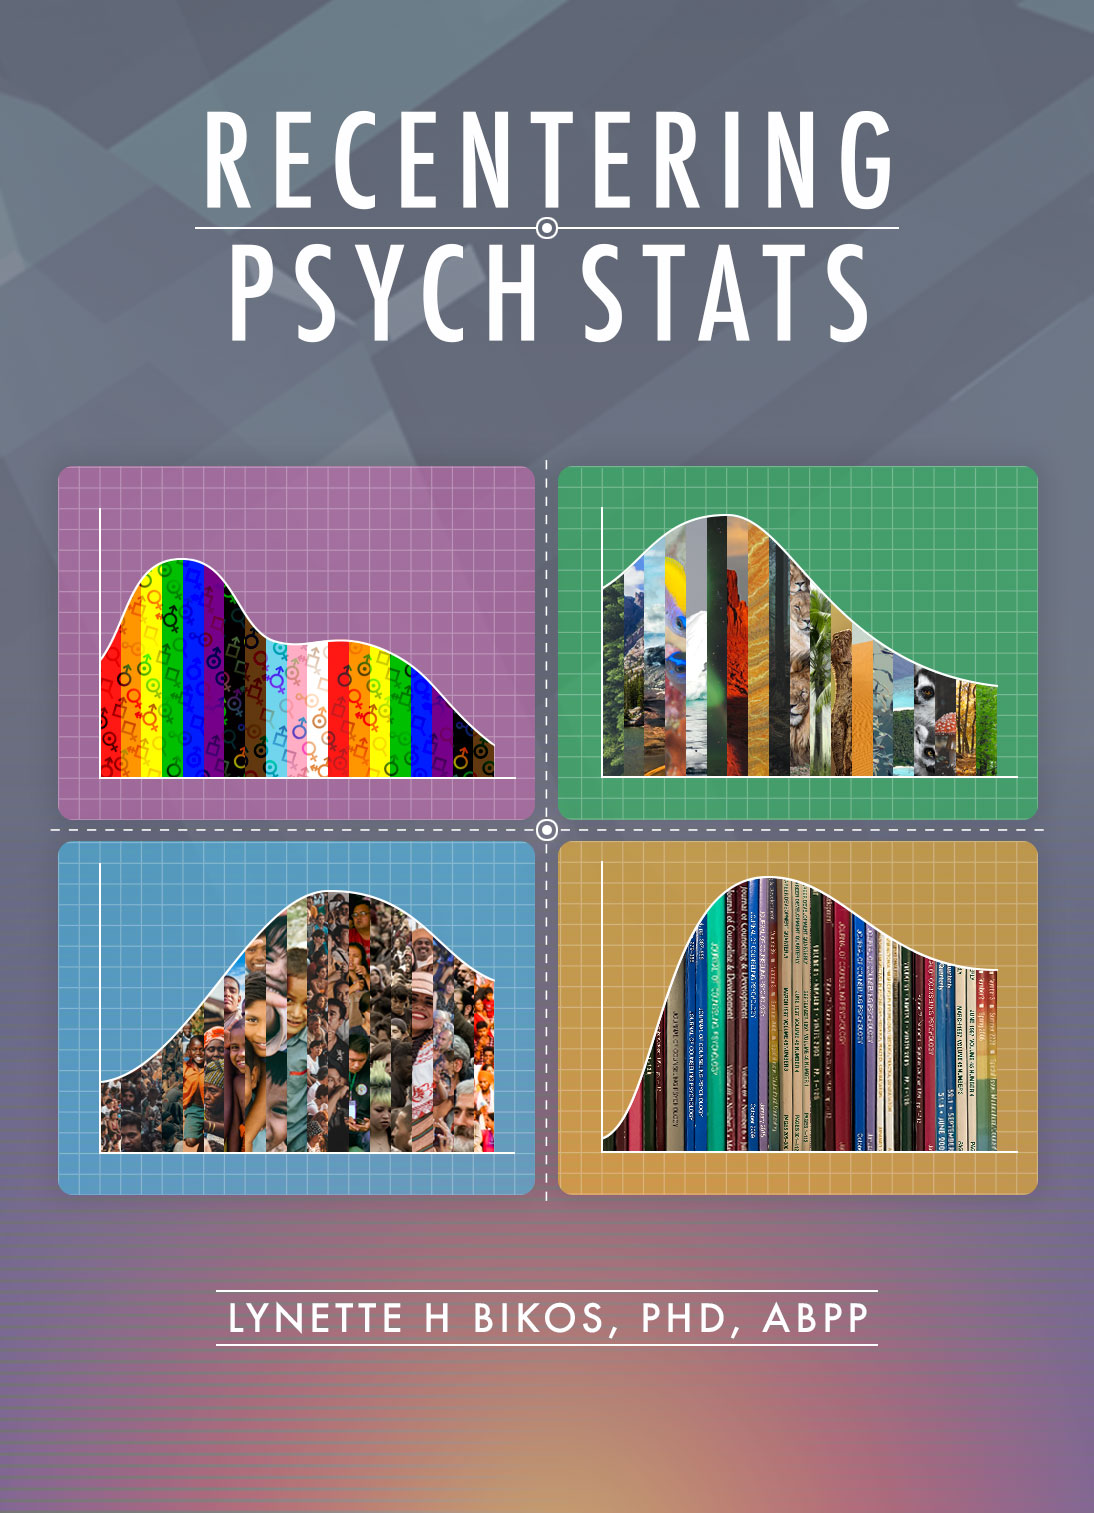
\includegraphics{images/ReCenterPsychStats-bookcover2.jpg} This open education resource is available in three formats:

\begin{itemize}
\tightlist
\item
  Formatted as an \href{https://lhbikos.github.io/ReCenterPsychStats/}{html book} via GitHub Pages
\item
  As a \href{https://github.com/lhbikos/ReCenterPsychStats/blob/main/docs/ReCenterPsychStats.pdf}{PDF} available in the \href{https://github.com/lhbikos/ReCenterPsychStats/tree/main/docs}{docs} folder at the GitHub repository
\item
  As an \href{https://github.com/lhbikos/ReCenterPsychStats/blob/main/docs/ReCenterPsychStats.epub}{ebook} available in the \href{https://github.com/lhbikos/ReCenterPsychStats/tree/main/docs}{docs} folder at the GitHub repository
\item
  As a \href{https://github.com/lhbikos/ReCenterPsychStats/blob/main/docs/ReCenterPsychStats.docx}{Word document} available in the \href{https://github.com/lhbikos/ReCenterPsychStats/tree/main/docs}{docs} folder at the GitHub repository
\end{itemize}

All materials used in creating this OER are available at its \href{https://github.com/lhbikos/ReCenterPsychStats}{GitHub repo}.

As a perpetually-in-progress, open education resource, feedback is always welcome. This IRB-approved (SPU IRB \#202102010R, no expiration) \href{https://spupsych.az1.qualtrics.com/jfe/form/SV_0OnBLfut3VIOIS2}{Qualtrics-hosted survey} includes formal rating scales, open-ended text boxes, and a portal for uploading attachments (e.g., marked up PDFs). You are welcome to complete only the portions that are relevant to you.

\hypertarget{preface}{%
\chapter*{PREFACE}\label{preface}}


\textbf{If you are viewing this document, you should know that this is a book-in-progress. Early drafts are released for the purpose teaching my classes and gaining formative feedback from a host of stakeholders. The document was last updated on 22 Jul 2023}. Emerging volumes on other statistics are posted on the \href{https://lhbikos.github.io/BikosRVT/ReCenter.html}{ReCentering Psych Stats} page at my research team's website.

\href{https://spu.hosted.panopto.com/Panopto/Pages/Viewer.aspx?id=859e5312-abdb-4db8-8779-b00c00feae47}{Screencasted Lecture Link}

\href{https://youtu.be/yy0z85Wla7o}{YouTube Lecture Link}

To \emph{center} a variable in regression means to set its value at zero and interpret all other values in relation to this reference point. Regarding race and gender, researchers often center male and White at zero. Further, it is typical that research vignettes in statistics textbooks are similarly seated in a White, Western (frequently U.S.), heteronormative, framework. The purpose of this project is to create a set of open educational resources (OER) appropriate for doctoral and post-doctoral training that contribute to a socially responsive pedagogy -- that is, it contributes to justice, equity, diversity, and inclusion.

Statistics training in doctoral programs are frequently taught with fee-for-use programs (e.g., SPSS/AMOS, SAS, MPlus) that may not be readily available to the post-doctoral professional. In recent years, there has been an increase and improvement in R packages (e.g., \emph{psych}, \emph{lavaan}) used for analyses common to psychological research. Correspondingly, many graduate programs are transitioning to statistics training in R (free and open source). This is a challenge for post-doctoral psychologists who were trained with other software. This OER will offer statistics training with R and be freely available (specifically in a GitHub repository and posted through GitHub Pages) under a Creative Commons Attribution - Non Commercial - Share Alike license {[}CC BY-NC-SA 4.0{]}.

Training models for doctoral programs in health service psychology are commonly scholar-practitioner, scientist-practitioner, or clinical-scientist. An emerging model, the \emph{scientist-practitioner-advocacy} training model, incorporates social justice advocacy so that graduates are equipped to recognize and address the sociocultural context of oppression and unjust distribution of resources and opportunities \citep{mallinckrodt_scientist-practitioner-advocate_2014}. In statistics textbooks, the use of research vignettes engages the learner around a tangible scenario for identifying independent variables, dependent variables, covariates, and potential mechanisms of change. Many students recall examples in Field's \citeyearpar{field_discovering_2012} popular statistics text: Viagra to teach one-way ANOVA, beer goggles for two-way ANOVA, and bushtucker for repeated measures. What if the research vignettes were more socially responsive?

In this OER, research vignettes will be from recently published articles where:

\begin{itemize}
\tightlist
\item
  the author's identity is from a group where scholarship is historically marginalized (e.g., BIPOC, LGBTQ+, LMIC{[}low-middle income countries{]}),
\item
  the research is responsive to issues of justice, equity, inclusion, diversity,
\item
  the lesson's statistic is used in the article, and
\item
  there is sufficient information in the article to simulate the data for the chapter example(s) and practice problem(s); or it is publicly available.
\end{itemize}

In training for multicultural competence, the saying, ``A fish doesn't know that it's wet'' is often used to convey the notion that we are often unaware of our own cultural characteristics. In recent months and years, there has been an increased awakening to institutional and systemic factors that contribute to discrimination as a function of race, gender, nationality, class, and so forth. Queuing from the water metaphor, I am hopeful that a text that is recentered in the ways I have described can contribute to \emph{changing the water} in higher education and in the profession of psychology.

\hypertarget{copyright-with-open-access}{%
\section*{Copyright with Open Access}\label{copyright-with-open-access}}


This book is published under a a Creative Commons Attribution-NonCommercial-ShareAlike 4.0 International License. This means that this book can be reused, remixed, retained, revised and redistributed (including commercially) as long as appropriate credit is given to the authors. If you remix, or modify the original version of this open textbook, you must redistribute all versions of this open textbook under the same license: CC BY-SA 4.0.

A \href{https://github.com/lhbikos/ReCenterPsychStats}{GitHub open-source repository} contains all of the text and source code for the book, including data and images.

\hypertarget{acknowledgements}{%
\chapter*{ACKNOWLEDGEMENTS}\label{acknowledgements}}


As a doctoral student at the University of Kansas (1992-1996), I learned that ``a foreign language'' was a graduation requirement. \emph{Please note that as one who studies the intersections of global, vocational, and sustainable psychology, I regret that I do not have language skills beyond English.} This could have been met with credit from high school, but my rural, mid-Missouri high school did not offer such classes. This requirement would have typically been met with courses taken during an undergraduate program -- but my non-teaching degree in the University of Missouri's School of Education was exempt from this. The requirement could have also been met with a computer language (FORTRAN, C++) -- but I did not have any of those either. There was a tiny footnote on my doctoral degree plan that indicated that a 2-credit course, ``SPSS for Windows'' would substitute for the language requirement. Given that it was taught by my one of my favorite professors, I readily signed up. As it turns out, Samuel B. Green, PhD, was using the course to draft chapters in the textbook \citep{green_using_2017} that has been so helpful for so many. Unfortunately, Drs. Green (1947 - 2018) and Salkind (1947 - 2017) are no longer with us. I have worn out numerous versions of their text. Another favorite text of mine has been Dr.~Barbara Byrne's \citeyearpar{byrne_structural_2016}, ``Structural Equation Modeling with AMOS.'' I loved the way she worked through each problem and paired it with a published journal article, so that the user could see how the statistical evaluation fit within the larger project/article. I took my tea-stained text with me to a workshop she taught at APA and was proud of the signature she added to it. Dr.~Byrne created SEM texts for a number of statistical programs (e.g., LISREL, EQS, MPlus). As I was learning R, I wrote Dr.~Byrne, asking if she had an edition teaching SEM/CFA with R. She promptly wrote back, saying that she did not have the bandwidth to learn a new statistics package. We lost Dr.~Byrne in December 2020. I am so grateful to these role models for their contributions to my statistical training. I am also grateful for the doctoral students who have taken my courses and are continuing to provide input for how to improve the materials.

The inspiration for training materials that re*center statistics and research methods came from the \href{https://www.academics4blacklives.com/}{Academics for Black Survival and Wellness Initiative}. This project, co-founded by Della V. Mosley, Ph.D., and Pearis L. Bellamy, M.S., made clear the necessity and urgency for change in higher education and the profession of psychology.

At very practical levels, I am indebted to SPU's Library, and more specifically, SPU's Education, Technology, and Media Department. Assistant Dean for Instructional Design and Emerging Technologies, R. John Robertson, MSc, MCS, has offered unlimited consultation, support, and connection. Senior Instructional Designer in Graphics \& Illustrations, Dominic Wilkinson, designed the logo and bookcover. Psychology and Scholarly Communications Librarian, Kristin Hoffman, MLIS, has provided consultation on topics ranging from OERS to citations. I am alo indebted to Associate Vice President, Teaching and Learning at Kwantlen Polytechnic University, Rajiv Jhangiani, PhD. Dr.~Jhangiani's text \citeyearpar{jhangiani_research_2019} was the first OER I ever used and I was grateful for his encouraging conversation.

Financial support for this project has been provided the following:

\begin{itemize}
\tightlist
\item
  \emph{Call to Action on Equity, Inclusion, Diversity, Justice, and Social Responsivity Request for Proposals} grant from the Association of Psychology Postdoctoral and Internship Centers (2021-2022).
\item
  \emph{Diversity Seed Grant}, Office of Inclusive Excellence and Advisory Council for Diversity and Reconciliation (ACDR), Seattle Pacific University.
\item
  \emph{ETM Open Textbook \& OER Development Funding}, Office of Education, Technology, \& Media, Seattle Pacific University.\texttt{\{r\ include=FALSE\}\ \#\ automatically\ create\ a\ bib\ database\ for\ R\ packages\ knitr::write\_bib(c(\ \ \ .packages(),\ \textquotesingle{}bookdown\textquotesingle{},\ \textquotesingle{}knitr\textquotesingle{},\ \textquotesingle{}rmarkdown\textquotesingle{}\ ),\ \textquotesingle{}packages.bib\textquotesingle{})}
\end{itemize}

\hypertarget{ReCintro}{%
\chapter{Introduction}\label{ReCintro}}

\href{https://spu.hosted.panopto.com/Panopto/Pages/Viewer.aspx?pid=cc9b7c0d-e5c3-4e4e-a469-acf7013ee761}{Screencasted Lecture Link}

\hypertarget{what-to-expect-in-each-chapter}{%
\section{What to expect in each chapter}\label{what-to-expect-in-each-chapter}}

This textbook is intended as \emph{applied,} in that a primary goal is to help the scientist-practitioner-advocate use a variety of statistics in research problems and \emph{writing them up} for a program evaluation, dissertation, or journal article. In support of that goal, I try to provide just enough conceptual information so that the researcher can select the appropriate statistic (i.e., distinguishing between when ANOVA is appropriate and when regression is appropriate) and assign variables to their proper role (e.g., covariate, moderator, mediator).

This conceptual approach does include occasional, step-by-step, \emph{hand-calculations} (using R to do the math for us) to provide a \emph{visceral feeling} of what is happening within the statistical algorithm that may be invisible to the researcher. Additionally, the conceptual review includes a review of the assumptions about the characteristics of the data and research design that are required for the statistic.

Statistics can be daunting, so I have worked hard to establish a \emph{workflow} through each analysis. When possible, I include a flowchart that is referenced frequently in each chapter and assists the researcher keep track of their place in the many steps and choices that accompany even the simplest of analyses.

As with many statistics texts, each chapter includes a \emph{research vignette.} Somewhat unique to this resource is that the vignettes are selected from recently published articles. Each vignette is chosen with the intent to meet as many of the following criteria as possible:

\begin{itemize}
\tightlist
\item
  the statistic that is the focus of the chapter was properly used in the article,
\item
  the author's identity is from a group where scholarship is historically marginalized (e.g., BIPOC, LGBTQ+, LMIC {[}low middle income countries{]}),
\item
  the research has a justice, equity, inclusion, diversity, and social responsivity focus and will contribute positively to a social justice pedagogy, and
\item
  there is sufficient information in the article to simulate the data for the chapter example(s) and practice problem(s); or the data is available in a repository.
\end{itemize}

In each chapter we employ \emph{R} packages that will efficiently calculate the statistic and the dashboard of metrics (e.g., effect sizes, confidence intervals) that are typically reported in psychological science.

\hypertarget{strategies-for-accessing-and-using-this-oer}{%
\section{Strategies for Accessing and Using this OER}\label{strategies-for-accessing-and-using-this-oer}}

There are a number of ways you can access this resource. You may wish to try several strategies and then select which works best for you. I demonstrate these in the screencast that accompanies this chapter.

\begin{enumerate}
\def\labelenumi{\arabic{enumi}.}
\item
  Simply follow along in your preferred format of the book (html, PDF, or ebook) and then

  \begin{itemize}
  \tightlist
  \item
    open a fresh .rmd file of your own, copying (or retyping) the script and running it
  \end{itemize}
\item
  Locate the original documents at the \href{https://github.com/lhbikos/ReCenterPsychStats}{GitHub repository}. You can

  \begin{itemize}
  \tightlist
  \item
    open them to simply take note of the ``behind the scenes'' script
  \item
    copy/download individual documents that are of interest to you
  \item
    clone a copy of the entire project to your own GitHub site and further download it (in its entirety) to your personal workspace. The \href{https://desktop.github.com/}{GitHub Desktop app} makes this easy!
  \end{itemize}
\item
  Listen to the accompanying lectures (I think sound best when the speed is 1.75). The lectures are being recorded in Panopto and should include the closed captioning.
\item
  Each time the book is updated, new .docx (Microsoft Word), PDF (Adobe Acrobat), and ebook(EPUB File) versions are also createdt. You can access these in the ``docs'' folder at the \href{https://github.com/lhbikos/ReCenterPsychStats}{GitHub repository}.
\item
  Provide feedback to me! If you fork a copy to your own GitHub repository, you can

  \begin{itemize}
  \tightlist
  \item
    open up an editing tool and mark up the document with your edits,
  \item
    start a discussion by leaving comments/questions, and then
  \item
    sending them back to me by committing and saving. I get an e-mail notiying me of this action. I can then review (accepting or rejecting) them and, if a discussion is appropriate, reply back to you.
  \item
    I am also seeking peer-review feedback at this \href{https://spupsych.az1.qualtrics.com/jfe/form/SV_0OnBLfut3VIOIS2}{Qualtrics-hosted survey}. You are welcome to complete only the portions that are relevant to you.
  \end{itemize}
\end{enumerate}

\hypertarget{if-you-are-new-to-r}{%
\section{If You are New to R}\label{if-you-are-new-to-r}}

R can be oveRwhelming. Jumping right into advanced statistics might not be the easiest way to start. The \href{https://lhbikos.github.io/ReCenterPsychStats/Ready.html}{Ready\_Set\_R}lesson of this volume provides an introduction and the \href{https://lhbikos.github.io/ReCenterPsychStats/waRmups.html}{waRming up}lesson walks through simple data preparation and descriptive statistics.

In the remaining lessons, I have attempted to provide complete code for every step of the process, starting with uploading the data. To help explain what R script is doing, I sometimes write it in the chapter text; sometimes leave hashtagged-comments in the chunks; and, particularly in the accompanying screencasted lectures, try to take time to narrate what the R script is doing.

I've found that, somewhere on the internet, there's almost always a solution to what I'm trying to do. I am frequently stuck and stumped and have spent hours searching the internet for even the tiniest of tasks. When you watch my videos, you may notice that in my R studio, there is a ``scRiptuRe'' file. I take notes on the solutions and scripts here -- using keywords that are meaningful to me so that when I need to repeat the task, I can hopefully search my own prior solutions and find a fix or a hint. You may also find it useful to create a working document of your own tips and tricks.

\hypertarget{introduction-to-the-data-set-used-for-homeworked-examples}{%
\section{Introduction to the Data Set Used for Homeworked Examples}\label{introduction-to-the-data-set-used-for-homeworked-examples}}

\href{}{Screencast Link}

This section of the Appendix is designed as a streamlined example of working the primary statistic from each lesson. This section is intended to be helpful in two ways:

\begin{itemize}
\tightlist
\item
  The worked example focuses on the operations and interpretations and more closely mimics ``how you would work a problem in real life.''
\item
  The grading rubric from the end of each lesson serves as the outline for the process.
\item
  This dataset could be used for the practice problems. For homework that you submit for grading, please choose \emph{different variables} than the ones worked in the examples.
\end{itemize}

\hypertarget{the-data-set}{%
\subsection{The Data Set}\label{the-data-set}}

The dataset used in the ``homeworked'' examples is from my own research. Along long with the pre-registration and codebooks, it is publicly available on the Open Science Framework (OSF): \url{https://osf.io/z84kh/} I have also provided a copy of it in the GitHub repository that hosts the ReCentering Psych Stats OER.

This data is from an IRB-approved study. The informed consent of the IRB specified that the data could be used in research as well as in teaching demonstrations and would be made available to the general public. You may notice there are student- and teacher- IDs. These numbers are *not** the institution's identification numbers. Rather, they have been further anonymized.

The purpose of the research project was to evaluate efforts to recenter -- in a socially responsive way -- courses in the statistics and research methods sequence in scientist-practitioner psychology (PhD) programs. The recentering occurred in two phases: (a) a transition from SPSS to R and (b) an explicit recentering. Data were from end-of-course evaluations three courses I taught: Research Methods I: Analysis of Variance {[}ANOVA{]}, Research Methods III: Multivariate Modeling {[}multivariate{]}, and Research Methods IV: Psychometrics/Theory of Test Construction {[}psychometrics{]}) that were offered 2017 through 2022.

Because students could contribute up to three course evaluations, each, multilevel modeling was used for the primary analyses. The nature of the data, though, allows me to demonstrate all of the statistics utilized the OER with this data. For each analysis, I have tried to derive a sensible question that \emph{could be} answered by the data. In-so-doing, I try to point out when the alignment of research question and statistic is less than ideal.

The data file is titled \emph{ReC.rds} and can be retrieved with this code:

\begin{Shaded}
\begin{Highlighting}[]
\NormalTok{dfReC }\OtherTok{\textless{}{-}} \FunctionTok{readRDS}\NormalTok{(}\StringTok{"ReC.rds"}\NormalTok{)}
\end{Highlighting}
\end{Shaded}

The following can serve as a codebook:

\begin{longtable}[]{@{}
  >{\raggedright\arraybackslash}p{(\columnwidth - 4\tabcolsep) * \real{0.1702}}
  >{\raggedright\arraybackslash}p{(\columnwidth - 4\tabcolsep) * \real{0.5638}}
  >{\raggedright\arraybackslash}p{(\columnwidth - 4\tabcolsep) * \real{0.2660}}@{}}
\toprule\noalign{}
\begin{minipage}[b]{\linewidth}\raggedright
Variable
\end{minipage} & \begin{minipage}[b]{\linewidth}\raggedright
Definition or Description
\end{minipage} & \begin{minipage}[b]{\linewidth}\raggedright
Scaling
\end{minipage} \\
\midrule\noalign{}
\endhead
\bottomrule\noalign{}
\endlastfoot
deID & Anonymized identification for each student Each student could contribute up to three course evaluations & Nominal/factor \\
CourseID & Unique number for each course taught (i.e., ANOVA has unique numbers across department and year). & Nominal/factor \\
Dept & CPY (Clinical Psychology), ORG (Industrial Organizational Psychology) & Nominal/factor \\
Course & ANOVA (analysis of variance), Multivariate (multivariate modeling), Psychometrics (psychometrics/theory of test construction), taught in that order & Nominal/factor \\
StatsPkg & SPSS, R & Nominal/factor \\
Centering & Pre (before explicit recentering), Re (included explicit recentering) & Nominal/factor \\
Year & Calendar year in which the course was taught & Calendrical time \\
Quarter & Academic term in which course was taught (fall, winter, spring) & Nominal/factor \\
ProgramYear & A potential confound to the study. During the changes from SPSS to R and the explicit recentering, the program was also moving the stats sequence from the second to the first year of the doctoral program. First = course taken during first year; Second = course taken during second year; Transition = course taken during the transition period. & Nominal/factor \\
SPFC.Decolonize.Opt.Out & Students were given the opportunity to exclude their data from analysis. Such data was removed prior to any analysis and not included in this set. & Character \\
\end{longtable}

COURSE EVALUATION ITEMS; 5-point Likert scaling from 1(\emph{strongly disagree}) to 5(\emph{strongly agree}). Higher scores are more favorable evaluations.

\begin{longtable}[]{@{}
  >{\raggedright\arraybackslash}p{(\columnwidth - 2\tabcolsep) * \real{0.1905}}
  >{\raggedright\arraybackslash}p{(\columnwidth - 2\tabcolsep) * \real{0.8095}}@{}}
\toprule\noalign{}
\begin{minipage}[b]{\linewidth}\raggedright
Variable
\end{minipage} & \begin{minipage}[b]{\linewidth}\raggedright
Complete Item
\end{minipage} \\
\midrule\noalign{}
\endhead
\bottomrule\noalign{}
\endlastfoot
IncrInterest & My interest in the subject matter increased over the span of the course. \\
IncrUnderstanding & My understanding of the subject matter increased over the span of the course. \\
ValObjectives & This course has objectives that are valuable in furthering my education. \\
ApprAssignments & This course has had an appropriate workload, given the course objectives. \\
EffectiveAnswers & The instructor has effectively answered student questions. \\
Respectful & The instructor has shown respect to students. \\
ClearResponsibilities & The instructor has made student responsibilities clear. \\
Feedback & The instructor has provided feedback to me about my learning progress. \\
OvInstructor & My overall rating of this instructor for this course is: \\
MultPerspectives & The instructor has helped students consider issues from multiple perspectives, where applicable. \\
OvCourse & My overall rating of the course content is: \\
InclsvClssrm & The instructor has been intentional in fostering an inclusive classroom for students with diverse backgrounds and abilities. \\
DEIintegration & The instructor has, when appropriate, discussed the relationships between race/ethnicity/culture and course content. \\
ClearPresentation & The instructor has presented course material clearly. \\
ApprWorkload & This course has had an appropriate workload, given the course objectives. \\
MyContribution & My overall rating of my contribution in this course is: \\
InspiredInterest & The instructor has inspired student interest in the subject matter of this course. \\
Faith & The instructor has, when appropriate, discussed the relationship between the Christian faith and course content. \\
EquitableEval & The instructor used methods of evaluating student course work that were equitable. \\
ClearOrganization & This course has had a clear overall organization. \\
RegPrepare & I regularly read, reviewed, visited/logged on, or completed assigned readings and tasks. \\
EffectiveLearning & This course has consisted of course activities/tasks that were effective in helping me learn (e.g., discussions, readings, assignments, labs, or other activities). \\
AccessibleInstructor & The instructor has been accessible (e.g., discussion sessions, virtual office hours, phone, chat, email, online forum or conference, etc.). \\
\end{longtable}

From these variables, I created three scales to assess valued by the student (Valued), traditional pedagogy (TradPed), and socially responsive pedagogy (SRped). I will use these in the demonstrations.

\begin{itemize}
\item
  \textbf{Valued by the student} includes the items: ValObjectives, IncrUnderstanding, IncrInterest
\item
  \textbf{Traditional pedagogy} includes the items: ClearResponsibilities, EffectiveAnswers, Feedback, ClearOrganization, ClearPresentation
\item
  \textbf{Socially responsive pedagogy} includes the items: InclusvClassrm, EquitableEval, MultPerspectives, DEIintegration
\end{itemize}

In the examples where the scale scores are used, I provide code for calculating the means.

Here's how to import the data:

\begin{Shaded}
\begin{Highlighting}[]
\NormalTok{ReCdf }\OtherTok{\textless{}{-}} \FunctionTok{readRDS}\NormalTok{(}\StringTok{"ReC.rds"}\NormalTok{)}
\end{Highlighting}
\end{Shaded}

\hypertarget{Ready}{%
\chapter{Ready\_Set\_R}\label{Ready}}

\href{https://spu.hosted.panopto.com/Panopto/Pages/Viewer.aspx?pid=6b27a60c-edcb-4565-aaf1-ad890174586e}{Screencasted Lecture Link}

With the goal of creating a common, system-wide approach to using the platform, this lesson was originally created for Clinical and Industrial-Organizational doctoral students who are entering the ``stats sequence.'' I hope it will be useful for others (e.g., faculty, post-doctoral researchers, and practitioners) who are also making the transition to R.

\hypertarget{navigating-this-lesson}{%
\section{Navigating this Lesson}\label{navigating-this-lesson}}

There is about 45 minutes of lecture.

While the majority of R objects and data you will need are created within the R script that sources the chapter, occasionally there are some that cannot be created from within the R framework. Additionally, sometimes links fail. All original materials are provided at the \href{https://github.com/lhbikos/ReCenterPsychStats}{Github site} that hosts the book. More detailed guidelines for ways to access all these materials are provided in the OER's \protect\hyperlink{ReCintro}{introduction}

\hypertarget{learning-objectives}{%
\subsection{Learning Objectives}\label{learning-objectives}}

Learning objectives from this lecture include the following:

\begin{itemize}
\tightlist
\item
  Downloading/installing R's parts and pieces.
\item
  Using R-Markdown as the interface for running R analyses and saving the script.
\item
  Recognizing and adopting best practices for ``R hygiene.''
\item
  Identifying effective strategies for troubleshooting R hiccups.
\end{itemize}

\hypertarget{downloading-and-installing-r}{%
\section{downloading and installing R}\label{downloading-and-installing-r}}

\hypertarget{so-many-parts-and-pieces}{%
\subsection{So many paRts and pieces}\label{so-many-parts-and-pieces}}

Before we download R, it may be helpful to review some of R's many parts and pieces.

The base software is free and is available \href{https://www.r-project.org/}{here}

Because R is already on my machine (and because the instructions are sufficient), I will not walk through the demo, but I will point out a few things.

\begin{itemize}
\tightlist
\item
  The ``cran'' (I think ``cranium'') is the \emph{Comprehensive R Archive Network.} In order for R to run on your computer, you have to choose a location -- and it should be geographically ``close to you.''

  \begin{itemize}
  \tightlist
  \item
    Follow the instructions for your operating system (Mac, Windows, Linux)
  \item
    You will see the results of this download on your desktop (or elsewhere if you chose to not have it appear there) but you won't ever use R through this platform.
  \end{itemize}
\item
  \href{https://www.rstudio.com/products/RStudio/}{R Studio} is the way in which we operate R. It's a separate download. Choose the free, desktop, option that is appropriate for your operating system:\\
\item
  \emph{R Markdown} is the way that many analysts write \emph{script}, conduct analyses, and even write up results. These are saved as .rmd files.

  \begin{itemize}
  \tightlist
  \item
    In R Studio, open an R Markdown document through File/New File/R Markdown
  \item
    Specify the details of your document (title, author, desired ouput)
  \item
    In a separate step, SAVE this document (File/Save{]} into a NEW FILE FOLDER that will contain anything else you need for your project (e.g., the data).
  \item
    \emph{Packages} are at the heart of working in R. Installing and activating packages require writing script.
  \end{itemize}
\end{itemize}

\textbf{Note} If you are working on an \emph{enterprise-owned machine} (e.g,. in my specific context, if you are a faculty/staff or have a lab with institution-issued laptops) there can be complications caused by how documents are stored. In recent years we have found that letting the computer choose where to load base R, R Studio, and the packages generally works. The trick is to save R projects (i.e., folder with .rmd files and data) into the OneDrive folder that syncs to your computer. If you have difficulty knitting that is unrelated to code/script (which you can evaluate by having a classmate or colleague successfully knit on their machine), it is likely because you have saved the files to the local hard drive and not OneDrive. If you continue to have problems I recommend consulting with your computer and technology support office.

\hypertarget{orienting-to-r-studio-focusing-only-on-the-things-we-will-be-using-first-and-most-often}{%
\subsection{oRienting to R Studio (focusing only on the things we will be using first and most often)}\label{orienting-to-r-studio-focusing-only-on-the-things-we-will-be-using-first-and-most-often}}

R Studio is organized around four panes. These can be re-sized and rearranged to suit your personal preferences.

\begin{itemize}
\tightlist
\item
  Upper right window

  \begin{itemize}
  \tightlist
  \item
    Environment: lists the \emph{objects} that are available to you (e.g., dataframes)
  \end{itemize}
\item
  Lower right window

  \begin{itemize}
  \tightlist
  \item
    \emph{Files}: Displays the file structure in your computer's environment. Make it a practice to (a) organize your work in small folders and (b) navigate to that small folder that is holding your project when you are working on it.
  \item
    \emph{Packages}: Lists the packages that have been installed. If you navigate to a specific package, you will know if it is ``on'' because its box is checked. You can also access information about the package (e.g., available functions, examples of script used with the package) in this menu. This information opens in the ``Help'' window.
  \item
    The \emph{Viewer} and \emph{Plots} tabs will be useful, later, in some advanced statistics when we can simultaneously examine output and script in windows that are side-by-side.
  \end{itemize}
\item
  Upper left window

  \begin{itemize}
  \tightlist
  \item
    If you are using R Markdown, that file lives here and is composed of open space and chunks.
  \end{itemize}
\item
  Lower left window

  \begin{itemize}
  \tightlist
  \item
    R Studio runs in the Console (the background). Very occasionally, I can find useful troubleshooting information here.
  \item
    More commonly, I open my R Markdown document so that it takes up the whole screen.
  \end{itemize}
\end{itemize}

\hypertarget{best-practices}{%
\section{best pRactices}\label{best-practices}}

Many initial problems in R can be solved with good R hygiene. Here are some suggestions for basic practices. It can be tempting to ``skip this.'' However, in the first few weeks of class, these are the solutions I am presenting (and repeating, ad nauseum) to my students.

\hypertarget{everything-is-documented-in-the-.rmd-file}{%
\subsection{Everything is documented in the .rmd file}\label{everything-is-documented-in-the-.rmd-file}}

Although others do it differently, I put \emph{everything} in my .rmd file. That is, my R script includes code for importing data and opening packages. Additionally, I make notes about the choices I am making. Relatedly, I keep a ``bug log'' -- noting what worked and what did not work. I will also begin my APA style results section directly in the .rmd file.

Why do I do all this? Because when I return to my project hours or years later, I have a permanent record of very critical things like (a) where my data is located, (b) what version I was using, and (c) what package was associated with the functions.

\hypertarget{setting-up-the-file}{%
\subsection{Setting up the file}\label{setting-up-the-file}}

File organization is a critical key to success. In your computing environment:

\begin{itemize}
\tightlist
\item
  Create a project file folder.
\item
  Put the data file in it.
\item
  Open an R Markdown file.
\item
  Save it in the same file folder as the data.
\item
  When your data and .rmd files are in the same folder (not your desktop, but a specific folder) the data can be pulled into the .rmd file without creating a working directory.
\end{itemize}

\hypertarget{script-in-chunks-and-everything-else-in-the-inline-text-sections}{%
\subsection{Script in chunks and everything else in the ``inline text'' sections}\label{script-in-chunks-and-everything-else-in-the-inline-text-sections}}

The R Markdown document is an incredible tool for integrating text, tables, and analyses. This entire OER is written in R Markdown. A central feature of this is ``chunks.''

The only thing in the chunks should be script for running R. You can also hashtag comments so they won't run (but you can also write anything you want between chunks without using hashtags).

Syntax for simple formatting in the text (i.e., non-chunk) areas (e.g., using italics, making headings, bold) is found here: \url{https://rmarkdown.rstudio.com/authoring_basics.html}

``Chunks'' start and end with with three tic marks and will show up in a shaded box. Chunks have three symbols in their upper right. Those controls will disappear (and your script will not run) if you have replaced them with double or single quotation marks or one or more of the tics are missing.

The easiest way to insert a chunk is to use the INSERT/R command at the top of this editor box. You can also insert a chunk with the keyboard shortcut: CTRL/ALT/i

\begin{Shaded}
\begin{Highlighting}[]
\CommentTok{\# hashtags let me write comments to remind myself what I did here I}
\CommentTok{\# am simply demonstrating arithmetic (but I would normally be running}
\CommentTok{\# code)}
\DecValTok{2021} \SpecialCharTok{{-}} \DecValTok{1966}
\end{Highlighting}
\end{Shaded}

\begin{verbatim}
[1] 55
\end{verbatim}

\hypertarget{managing-packages}{%
\subsection{Managing packages}\label{managing-packages}}

As scientist-practitioners (and not coders), we will rely on \emph{packages} to do much of the work. At first you may feel overwhelmed about the large number of packages that are available. Soon, though, you will become accustomed to the ones most applicable to our work (e.g., psych, tidyverse, rstatix, apaTables).

Researchers treat packages differently. In these lectures, I list all the packages we will use in an opening chunk at the beginning of the lecture. When the hashtags are removed, the script will ask R to check to see if the package is installed on your machine. If it is, installation is skipped. If it is not, R installs it. Simply remove the hashtag to run the code the first time, then hashtag them back out so R is not always re-checking.

\begin{Shaded}
\begin{Highlighting}[]
\CommentTok{\# will install the package if not already installed}
\CommentTok{\# if(!require(psych))\{install.packages(\textquotesingle{}psych\textquotesingle{})\}}
\end{Highlighting}
\end{Shaded}

To make a package operable, you need to open it. There are two primary ways to do this. The first is to use the library function.

\begin{Shaded}
\begin{Highlighting}[]
\CommentTok{\#install.packages ("psych")}
\FunctionTok{library}\NormalTok{ (psych)}
\end{Highlighting}
\end{Shaded}

The second way is to place a double colon between the package and function. This second method has become my preferred practice because it helps me remember what package goes with each function. It can also prevent R hiccups when there are identical function names and R does not know which package to use. Below is an example where I might ask for descriptives from the psych package. Because I have not yet uploaded data, I have hashtagged it out, making the command inoperable.

\begin{Shaded}
\begin{Highlighting}[]
\CommentTok{\#psych::describe(mydata)}
\end{Highlighting}
\end{Shaded}

There are exceptions. One is the \emph{tidyverse} package. Some of my script uses pipes (\%\textgreater\%) and pipes require \emph{tidyverse} to be activated. This is why you will often see me call the \emph{tidyverse} package with the \emph{library()} function (as demonstrated above.)

\hypertarget{upload-the-data}{%
\subsection{Upload the data}\label{upload-the-data}}

When imported (or simulated) properly, data will appear as an object in the global environment.

In the context of this OER, I will be simulating data in each lesson for immediate use in the lesson. This makes this web-based OER more \emph{portable.} This also means that when working the problems in the chapter we do notneed to (a) write the data to a file or (b) import data from files. Because these are essential skills, I will demonstrate this process here -- starting with simulating data.

At this point, simulating data is beyond the learning goals I have established for the chapter. I do need to include the code so that we get some data. The data I am simulating is used in the \protect\hyperlink{oneway}{one-way ANOVA lesson}. The data is from the Tran and Lee \citeyearpar{tran_you_2014} random clinical trial.

In this simulation, I am simply creating an ID number, a condition (High, Low, Control), and a score on the dependent variable, ``Accurate.'' More information about this study is included in the \protect\hyperlink{oneway}{one-way ANOVA chapter}.

\begin{Shaded}
\begin{Highlighting}[]
\CommentTok{\# Note, this simulation results in a different datset than is in the}
\CommentTok{\# OnewayANOVA lesson sets a random seed so that we get the same}
\CommentTok{\# results each time}
\FunctionTok{set.seed}\NormalTok{(}\DecValTok{2021}\NormalTok{)}
\CommentTok{\# sample size, M and SD for each group}
\NormalTok{Accurate }\OtherTok{\textless{}{-}} \FunctionTok{c}\NormalTok{(}\FunctionTok{rnorm}\NormalTok{(}\DecValTok{30}\NormalTok{, }\AttributeTok{mean =} \FloatTok{1.18}\NormalTok{, }\AttributeTok{sd =} \FloatTok{0.8}\NormalTok{), }\FunctionTok{rnorm}\NormalTok{(}\DecValTok{30}\NormalTok{, }\AttributeTok{mean =} \FloatTok{1.83}\NormalTok{,}
    \AttributeTok{sd =} \FloatTok{0.58}\NormalTok{), }\FunctionTok{rnorm}\NormalTok{(}\DecValTok{30}\NormalTok{, }\AttributeTok{mean =} \FloatTok{1.76}\NormalTok{, }\AttributeTok{sd =} \FloatTok{0.56}\NormalTok{))}
\CommentTok{\# set upper bound for DV}
\NormalTok{Accurate[Accurate }\SpecialCharTok{\textgreater{}} \DecValTok{3}\NormalTok{] }\OtherTok{\textless{}{-}} \DecValTok{3}
\CommentTok{\# set lower bound for DV}
\NormalTok{Accurate[Accurate }\SpecialCharTok{\textless{}} \DecValTok{0}\NormalTok{] }\OtherTok{\textless{}{-}} \DecValTok{0}
\CommentTok{\# IDs for participants}
\NormalTok{ID }\OtherTok{\textless{}{-}} \FunctionTok{factor}\NormalTok{(}\FunctionTok{seq}\NormalTok{(}\DecValTok{1}\NormalTok{, }\DecValTok{90}\NormalTok{))}
\CommentTok{\# name factors and identify how many in each group; should be in same}
\CommentTok{\# order as first row of script}
\NormalTok{COND }\OtherTok{\textless{}{-}} \FunctionTok{c}\NormalTok{(}\FunctionTok{rep}\NormalTok{(}\StringTok{"High"}\NormalTok{, }\DecValTok{30}\NormalTok{), }\FunctionTok{rep}\NormalTok{(}\StringTok{"Low"}\NormalTok{, }\DecValTok{30}\NormalTok{), }\FunctionTok{rep}\NormalTok{(}\StringTok{"Control"}\NormalTok{, }\DecValTok{30}\NormalTok{))}
\CommentTok{\# groups the 3 variables into a single df: ID, DV, condition}
\NormalTok{Acc\_sim30 }\OtherTok{\textless{}{-}} \FunctionTok{data.frame}\NormalTok{(ID, COND, Accurate)}
\end{Highlighting}
\end{Shaded}

At this point, this data lives only in this .rmd file after the above code is run. Although there are numerous ways to export and import data, I have a preference for two.

\hypertarget{to-and-from-.csv-files}{%
\subsubsection{To and from .csv files}\label{to-and-from-.csv-files}}

The first is to write the data to a .csv file. In your computer's environment (outside of R), these files are easily manipulated in Excel. I think of them as being ``Excel lite'' because although Excel can operate them, they lack some of the more advanced features of an Excel spreadsheet.

In the code below, I identify the R object ``Acc\_sim30'' and give it a file name, ``to\_CSV.csv''. This file name must have the .csv extension. I also indicate that it should preserve the column names (but ignore row names; since we don't have row names).

This file will save in the same folder as wherever you are using this .rmd file.

\begin{Shaded}
\begin{Highlighting}[]
\CommentTok{\# to write it to an outfile as a .csv}
\FunctionTok{write.table}\NormalTok{(Acc\_sim30, }\AttributeTok{file =} \StringTok{"to\_CSV.csv"}\NormalTok{, }\AttributeTok{sep =} \StringTok{","}\NormalTok{, }\AttributeTok{col.names =} \ConstantTok{TRUE}\NormalTok{,}
    \AttributeTok{row.names =} \ConstantTok{FALSE}\NormalTok{)}
\end{Highlighting}
\end{Shaded}

Importing this object back into the R environment can be accomplished with some simple code. For the sake of demonstration,

\begin{Shaded}
\begin{Highlighting}[]
\CommentTok{\# to save the df as an .csv (think \textquotesingle{}Excel lite\textquotesingle{}) file on your}
\CommentTok{\# computer; it should save in the same file as the .rmd file you are}
\CommentTok{\# working with}
\NormalTok{from\_CSV }\OtherTok{\textless{}{-}} \FunctionTok{read.csv}\NormalTok{(}\StringTok{"to\_CSV.csv"}\NormalTok{, }\AttributeTok{header =} \ConstantTok{TRUE}\NormalTok{)}
\end{Highlighting}
\end{Shaded}

The advantage of working with .csv files is that it is then easy to inspect and manipulate them outside of the R environment. The disadvantage of .csv files is that each time they are imported they lose any formatting you may have meticulously assigned to them.

\hypertarget{to-and-from-.rds-files}{%
\subsubsection{To and from .rds files}\label{to-and-from-.rds-files}}

While it is easy enough to rerun the code (or copy it from data prep .rmd and paste it into an .rmd you are using for advanced analysis), there is a better way! Saving the data as an R object preserves all of its characteristics.

\begin{Shaded}
\begin{Highlighting}[]
\CommentTok{\# to save the df as an .rds file on your computer; it should save in}
\CommentTok{\# the same file as the .rmd file you are working with}
\FunctionTok{saveRDS}\NormalTok{(Acc\_sim30, }\StringTok{"to\_Robject.rds"}\NormalTok{)}
\end{Highlighting}
\end{Shaded}

This file will save to your computer (and you can send it to colleagues). However, it is not easy to ``just open it'' in Excel. To open an .rds file and use it (whether you created it or it is sent to you by a colleague), use the following code:

\begin{Shaded}
\begin{Highlighting}[]
\NormalTok{from\_rds }\OtherTok{\textless{}{-}} \FunctionTok{readRDS}\NormalTok{(}\StringTok{"to\_Robject.rds"}\NormalTok{)}
\end{Highlighting}
\end{Shaded}

If you are the recipient of an R object, but want to view it as a .csv, simply import the .rds then use the above code to export it as a .csv.

\hypertarget{from-spss-files}{%
\subsubsection{From SPSS files}\label{from-spss-files}}

Your data may come to you in a variety of ways. One of the most common is SPSS. The \emph{foreign} package is popular for importing SPSS data. Below is code which would import an SPSS file \emph{if I had created one}. You'll see that this script is hashtagged out because I rarely use SPSS and do not have a handy file to demo.

\begin{Shaded}
\begin{Highlighting}[]
\CommentTok{\# opening an SPSS file requires the foreign package which I opened}
\CommentTok{\# earlier from\_SPSS \textless{}{-} foreign::read.spss (\textquotesingle{}SPSSdata.sav\textquotesingle{},}
\CommentTok{\# use.value.labels = TRUE, to.data.frame = TRUE)}
\end{Highlighting}
\end{Shaded}

\hypertarget{quick-demonstration}{%
\section{quick demonstRation}\label{quick-demonstration}}

Let's run some simple descriptives. In the script below, I am using the \emph{psych} package. Descriptive statistics will appear for all the data in the dataframe and the output will be rounded to three spaces. Note that rather than opening the psych package with the library function, I have used the double colon convention.

\begin{Shaded}
\begin{Highlighting}[]
\FunctionTok{round}\NormalTok{(psych}\SpecialCharTok{::}\FunctionTok{describe}\NormalTok{(Acc\_sim30), }\DecValTok{3}\NormalTok{)}
\end{Highlighting}
\end{Shaded}

\begin{verbatim}
         vars  n  mean    sd median trimmed   mad min max range  skew kurtosis
ID*         1 90 45.50 26.12  45.50   45.50 33.36   1  90    89  0.00    -1.24
COND*       2 90  2.00  0.82   2.00    2.00  1.48   1   3     2  0.00    -1.53
Accurate    3 90  1.52  0.68   1.55    1.54  0.70   0   3     3 -0.19    -0.34
           se
ID*      2.75
COND*    0.09
Accurate 0.07
\end{verbatim}

Because ``ID'' is the case ID and COND is the factor (high, low, control), the only variable for which this data is sensible is ``Accurate.'' Nonetheless, this provides an example of how to apply a package's function to a dataset. As we progress through the text we will learn how to manage the data so that we get the specific output we are seeking.

\hypertarget{the-knitted-file}{%
\section{the knitted file}\label{the-knitted-file}}

One of the coolest things about R Markdown is its capacity to \emph{knit} to HTML, PPT, or WORD.

\begin{itemize}
\tightlist
\item
  In this OER, I am writing the lessons in R markdown (.rmd files), with the package \emph{bookdown} as a helper, and knitting the files to .html, .doc, .pdf, and .epub formats.
\item
  The package \emph{papaja} is designed to prepare APA manuscripts where the writing, statistics, and references are all accomplished in a single file. This process contributes to replicability and reproducibility.
\item
  More detailed instructions for knitting to these formats are provided in the \href{https://lhbikos.github.io/extRas/}{extRas} mini-volume of \href{https://lhbikos.github.io/BikosRVT/ReCenter.html}{ReCentering Psych Stats}.
\end{itemize}

\hypertarget{troubleshooting-in-r-markdown}{%
\section{tRoubleshooting in R maRkdown}\label{troubleshooting-in-r-markdown}}

Hiccups are normal. Here are some ideas that I have found useful in getting unstuck.

\begin{itemize}
\tightlist
\item
  In a given set of operations, you must run/execute each piece of code in order: every, single, time. That is, all the packages have to be in your library and activated.

  \begin{itemize}
  \tightlist
  \item
    If you open an .rmd file, you cannot just scroll down to make a boxplot. You need to run any \emph{prerequisite} script (like loading files, putting the data in the global environment, etc.)
  \item
    Lost? Clear your global environment (broom icon in the upper right) and start over. Fresh starts are good.
  \end{itemize}
\item
  Your .rmd file and your data need to be stored in the same file folder. Make unique folders for each project (even if each contains only a few files).
\item
  If you have tried what seems apparent to you and cannot solve your challenge, do not wait long before typing warnings into a search engine. Odds are, you'll get some useful hints in a manner of seconds. Especially at first, these are common errors:

  \begin{itemize}
  \tightlist
  \item
    The package isn't loaded.
  \item
    The .rmd file hasn't been saved yet, or isn't saved in the same folder as the data.
  \item
    There are errors in punctuation or spelling.
  \end{itemize}
\item
  Restart R (it's quick -- not like restarting your computer). I frequently restart and clear my output and environment so that I can better track my order of operations.
\item
  If you receive an error indicating that a function isn't working or recognized, and you have loaded the package, type the name of the package in front of the function with two colons (e.g., psych::describe(df)). If multiple packages are loaded with functions that have the same name, R can get confused.
\end{itemize}

\hypertarget{just-why-have-we-transitioned-to-r}{%
\section{\texorpdfstring{just \emph{why} have we tRansitioned to R?}{just why have we tRansitioned to R?}}\label{just-why-have-we-transitioned-to-r}}

\begin{itemize}
\tightlist
\item
  It is (or at least it appears to be) the futuRe.
\item
  SPSS individual and site licenses are increasingly expensive and limited; that is, Mplus, AMOS, HLM, or R tools may also be needed. As package development for R is exploding, we have tools to ``do just about anything.''
\item
  Most graduate psychology programs are scientist/practitioner in nature and include training in ``high end'' statistics. Yet, many of your employing organizations will not have SPSS. R is a free, universally accessible program, that our graduates can use anywhere.
\end{itemize}

\hypertarget{strategies-for-success}{%
\section{stRategies for success}\label{strategies-for-success}}

\begin{itemize}
\tightlist
\item
  Engage with R, but don't let it overwhelm you.

  \begin{itemize}
  \tightlist
  \item
    The \emph{mechanical is also the conceptual}. Especially while it's \emph{simpler}, do try to retype the script into your own .rmd file and run it. Track down the errors you are making and fix them.
  \item
    If this stresses you out, move to simply copying the code into the .rmd file and running it. If you continue to have errors, you may have violated one of the best practices above (ask, ``Is the package activated?'' ``Are the data and .rmd files in the same place?'' ``Is all the prerequisite script run?'').
  \item
    Still overwhelmed? Keep moving forward by (retrieving the original .rmd file from the GitHub repository) opening a copy of the .rmd file and just ``run it along'' with the lecture. Spend your mental power trying to understand what each piece does so you can translate it for any homework assignments. My suggestions for practice are intended to be parallel to the lecture with no sneaky trix.
  \end{itemize}
\item
  Copy script that works elsewhere and replace it with your datafile, variables, and so forth.
\item
  The leaRning curve is steep, but not impossible. Gladwell \citeyearpar{gladwell_outliers_2008} taught us that it takes about 10,000 hours to get great at something (2,000 to get reasonably competent). Practice. Practice. Practice.
\item
  Updates to R, R Studio, and the packages are necessary, but can also be problematic. Sometimes updates cause programs/script to fail (e.g., ``X has been deprecated for version X.XX''). My personal practice is to update R, R Studio, and the packages a week or two before each academic term. I expect that

  \begin{itemize}
  \tightlist
  \item
    prior scripts may need to be updated or revised with package updates, and
  \item
    there will be incongruencies between base R, R Studio, and the packages.
  \end{itemize}
\item
  Embrace your downward dog. And square breathing. Also, walk away, then come back.
\end{itemize}

\hypertarget{resources-for-getting-started}{%
\section{Resources for getting staRted}\label{resources-for-getting-started}}

R for Data Science: \url{https://r4ds.had.co.nz/}

R Cookbook: \url{http://shop.oreilly.com/product/9780596809164.do}

R Markdown homepage with tutorials: \url{https://rmarkdown.rstudio.com/index.html}

R has cheatsheets for everything, here's the one for R Markdown: \url{https://www.rstudio.com/wp-content/uploads/2015/02/rmarkdown-cheatsheet.pdf}

R Markdown Reference guide: \url{https://www.rstudio.com/wp-content/uploads/2015/03/rmarkdown-reference.pdf}

Using R Markdown for writing reproducible scientific papers: \url{https://libscie.github.io/rmarkdown-workshop/handout.html}

Script for all of Field's text: \url{https://studysites.uk.sagepub.com/dsur/study/scriptfi.htm}

LaTeX equation editor: \url{https://www.codecogs.com/latex/eqneditor.php}

\hypertarget{practice-problems}{%
\section{Practice Problems}\label{practice-problems}}

The suggestions for practice in this lesson are foundational for starting work in R. If you struggle with any of these steps, I encourage you to get consultation from a peer, instructor, or a tutor.

\begin{longtable}[]{@{}
  >{\raggedright\arraybackslash}p{(\columnwidth - 4\tabcolsep) * \real{0.5493}}
  >{\centering\arraybackslash}p{(\columnwidth - 4\tabcolsep) * \real{0.2535}}
  >{\centering\arraybackslash}p{(\columnwidth - 4\tabcolsep) * \real{0.1972}}@{}}
\toprule\noalign{}
\begin{minipage}[b]{\linewidth}\raggedright
Assignment Component
\end{minipage} & \begin{minipage}[b]{\linewidth}\centering
Points Possible
\end{minipage} & \begin{minipage}[b]{\linewidth}\centering
Points Earned
\end{minipage} \\
\midrule\noalign{}
\endhead
\bottomrule\noalign{}
\endlastfoot
1. Download base R and R Studio & 5 & \_\_\_\_\_ \\
2. Open and save an .rmd (R Markdown) file in a ``sensible location'' on your computer & 5 & \_\_\_\_\_ \\
3. In the .rmd file, open a chunk and perform a simple mathematical operation of your choice (e.g., subtract your birth year from this year) & 5 & \_\_\_\_\_ \\
4. Install at least three packages; we will commonly use \emph{psych}, \emph{tidyverse}, \emph{dplyr}, \emph{knitr}, \emph{ggplot2}, \emph{ggpubr}) & 5 & \_\_\_\_\_ \\
5. Copy the simulation in this lesson to your .rmd file. Change the random seed and run the simulation. Save the resulting data as a .csv or .rds file \emph{in the same file as you saved the .rmd file}. & 5 & \_\_\_\_\_ \\
6. Clear your environment (broom in upper right). Open the simulated file that you saved. & 5 & \_\_\_\_\_ \\
7. Run the \emph{describe()} function from the \emph{psych} package with your simulated data that you imported from your local drive. & 5 & \_\_\_\_\_ \\
8. Demonstration/discussion with a grader. & 5 & \_\_\_\_\_ \\
\textbf{Totals} & 40 & \_\_\_\_\_ \\
\end{longtable}

\hypertarget{homeworked-example}{%
\section{Homeworked Example}\label{homeworked-example}}

\href{}{Screencast Link}

Several elements of the practice problems (i.e., download base R and R studio, open and save an r.rmd file) are not easily demonstrated and not replicated here. These are skipped.

\emph{If you wanted to use this example and dataset as a basis for a homework assignment, you could simply change the seed -- again. For a greater challenge, you could adjust the simulation to have different sample sizes, means, or standard deviations.}

\hypertarget{perform-a-simple-mathematical-operation}{%
\subsection{Perform a simple mathematical operation:}\label{perform-a-simple-mathematical-operation}}

In the .rmd file, open a chunk and perform a simple mathematical operation of your choice (e.g., subtract your birth year from this year).

\begin{Shaded}
\begin{Highlighting}[]
\DecValTok{2023} \SpecialCharTok{{-}} \DecValTok{1966}
\end{Highlighting}
\end{Shaded}

\begin{verbatim}
[1] 57
\end{verbatim}

\hypertarget{install-at-least-three-packages-we-will-commonly-use}{%
\subsection{Install at least three packages we will commonly use:}\label{install-at-least-three-packages-we-will-commonly-use}}

Below is code for installing three packages. Because continuous reinstallation can be problematic, I have hashtagged them so that they will not re-run.

\begin{Shaded}
\begin{Highlighting}[]
\CommentTok{\#install.packages("tidyverse")}
\CommentTok{\#install.packages("ggpubr")}
\CommentTok{\#install.packages("psych")}
\end{Highlighting}
\end{Shaded}

\hypertarget{copy-the-simulation-in-this-lesson-to-your-.rmd-file.-change-the-random-seed-and-run-the-simulation.}{%
\subsection{Copy the simulation in this lesson to your .rmd file. Change the random seed and run the simulation.}\label{copy-the-simulation-in-this-lesson-to-your-.rmd-file.-change-the-random-seed-and-run-the-simulation.}}

\begin{Shaded}
\begin{Highlighting}[]
\FunctionTok{set.seed}\NormalTok{(}\DecValTok{2023}\NormalTok{)}
\CommentTok{\# sample size, M and SD for each group}
\NormalTok{Accurate }\OtherTok{\textless{}{-}} \FunctionTok{c}\NormalTok{(}\FunctionTok{rnorm}\NormalTok{(}\DecValTok{30}\NormalTok{, }\AttributeTok{mean =} \FloatTok{1.18}\NormalTok{, }\AttributeTok{sd =} \FloatTok{0.8}\NormalTok{), }\FunctionTok{rnorm}\NormalTok{(}\DecValTok{30}\NormalTok{, }\AttributeTok{mean =} \FloatTok{1.83}\NormalTok{,}
    \AttributeTok{sd =} \FloatTok{0.58}\NormalTok{), }\FunctionTok{rnorm}\NormalTok{(}\DecValTok{30}\NormalTok{, }\AttributeTok{mean =} \FloatTok{1.76}\NormalTok{, }\AttributeTok{sd =} \FloatTok{0.56}\NormalTok{))}
\CommentTok{\# set upper bound for DV}
\NormalTok{Accurate[Accurate }\SpecialCharTok{\textgreater{}} \DecValTok{3}\NormalTok{] }\OtherTok{\textless{}{-}} \DecValTok{3}
\CommentTok{\# set lower bound for DV}
\NormalTok{Accurate[Accurate }\SpecialCharTok{\textless{}} \DecValTok{0}\NormalTok{] }\OtherTok{\textless{}{-}} \DecValTok{0}
\CommentTok{\# IDs for participants}
\NormalTok{ID }\OtherTok{\textless{}{-}} \FunctionTok{factor}\NormalTok{(}\FunctionTok{seq}\NormalTok{(}\DecValTok{1}\NormalTok{, }\DecValTok{90}\NormalTok{))}
\CommentTok{\# name factors and identify how many in each group; should be in same}
\CommentTok{\# order as first row of script}
\NormalTok{COND }\OtherTok{\textless{}{-}} \FunctionTok{c}\NormalTok{(}\FunctionTok{rep}\NormalTok{(}\StringTok{"High"}\NormalTok{, }\DecValTok{30}\NormalTok{), }\FunctionTok{rep}\NormalTok{(}\StringTok{"Low"}\NormalTok{, }\DecValTok{30}\NormalTok{), }\FunctionTok{rep}\NormalTok{(}\StringTok{"Control"}\NormalTok{, }\DecValTok{30}\NormalTok{))}
\CommentTok{\# groups the 3 variables into a single df: ID, DV, condition}
\NormalTok{Acc\_sim30B }\OtherTok{\textless{}{-}} \FunctionTok{data.frame}\NormalTok{(ID, COND, Accurate)}
\end{Highlighting}
\end{Shaded}

\hypertarget{save-the-resulting-data-as-a-.csv-or-.rds-file-in-the-same-file-as-you-saved-the-.rmd-file.}{%
\subsection{Save the resulting data as a .csv or .rds file in the same file as you saved the .rmd file.}\label{save-the-resulting-data-as-a-.csv-or-.rds-file-in-the-same-file-as-you-saved-the-.rmd-file.}}

You only need to save it as a .csv or .rds file. I have demonstrated both.

Saving as a .csv file

\begin{Shaded}
\begin{Highlighting}[]
\FunctionTok{write.table}\NormalTok{(Acc\_sim30B, }\AttributeTok{file =} \StringTok{"to\_CSVb.csv"}\NormalTok{, }\AttributeTok{sep =} \StringTok{","}\NormalTok{, }\AttributeTok{col.names =} \ConstantTok{TRUE}\NormalTok{,}
    \AttributeTok{row.names =} \ConstantTok{FALSE}\NormalTok{)}
\end{Highlighting}
\end{Shaded}

Saving as an .rds file

\begin{Shaded}
\begin{Highlighting}[]
\FunctionTok{saveRDS}\NormalTok{(Acc\_sim30B, }\StringTok{"to\_RobjectB.rds"}\NormalTok{)}
\end{Highlighting}
\end{Shaded}

\hypertarget{clear-your-environment-broom-in-upper-right.}{%
\subsection{Clear your environment (broom in upper right).}\label{clear-your-environment-broom-in-upper-right.}}

You only need to import the .csv or .rds file; I have demonstrated both. Open the .csv file from my local drive.

\begin{Shaded}
\begin{Highlighting}[]
\NormalTok{from\_CSV }\OtherTok{\textless{}{-}} \FunctionTok{read.csv}\NormalTok{(}\StringTok{"to\_CSVb.csv"}\NormalTok{, }\AttributeTok{header =} \ConstantTok{TRUE}\NormalTok{)}
\end{Highlighting}
\end{Shaded}

Open the .rds file from my local drive.

\begin{Shaded}
\begin{Highlighting}[]
\NormalTok{from\_rds }\OtherTok{\textless{}{-}} \FunctionTok{readRDS}\NormalTok{(}\StringTok{"to\_RobjectB.rds"}\NormalTok{)}
\end{Highlighting}
\end{Shaded}

\hypertarget{run-the-describe-function-from-the-psych-package-with-your-simulated-data-that-you-imported-from-your-local-drive.}{%
\subsection{Run the describe() function from the psych package with your simulated data that you imported from your local drive.}\label{run-the-describe-function-from-the-psych-package-with-your-simulated-data-that-you-imported-from-your-local-drive.}}

You only need to retrieve descriptives from the .csv or .rds file; I have demonstrated both.

\begin{Shaded}
\begin{Highlighting}[]
\NormalTok{psych}\SpecialCharTok{::}\FunctionTok{describe}\NormalTok{(from\_CSV)}
\end{Highlighting}
\end{Shaded}

\begin{verbatim}
         vars  n  mean    sd median trimmed   mad min max range  skew kurtosis
ID          1 90 45.50 26.12   45.5   45.50 33.36   1  90    89  0.00    -1.24
COND*       2 90  2.00  0.82    2.0    2.00  1.48   1   3     2  0.00    -1.53
Accurate    3 90  1.65  0.67    1.7    1.67  0.68   0   3     3 -0.29    -0.42
           se
ID       2.75
COND*    0.09
Accurate 0.07
\end{verbatim}

\begin{Shaded}
\begin{Highlighting}[]
\NormalTok{psych}\SpecialCharTok{::}\FunctionTok{describe}\NormalTok{(from\_rds)}
\end{Highlighting}
\end{Shaded}

\begin{verbatim}
         vars  n  mean    sd median trimmed   mad min max range  skew kurtosis
ID*         1 90 45.50 26.12   45.5   45.50 33.36   1  90    89  0.00    -1.24
COND*       2 90  2.00  0.82    2.0    2.00  1.48   1   3     2  0.00    -1.53
Accurate    3 90  1.65  0.67    1.7    1.67  0.68   0   3     3 -0.29    -0.42
           se
ID*      2.75
COND*    0.09
Accurate 0.07
\end{verbatim}

\hypertarget{preliminaries}{%
\chapter{Preliminary Analyses}\label{preliminaries}}

\href{https://spu.hosted.panopto.com/Panopto/Pages/Viewer.aspx?pid=97ec1420-3527-4204-8521-aeff0000afed}{Screencasted Lecture Link}

The beginning of any data analysis means familiarizing yourself with the data. Among other things, this includes producing and interpreting its distributional characteristics. In this lesson we mix common R operations for formatting, preparing, and analyzing the data with foundational statistical concepts in statistics.

\hypertarget{navigating-this-lesson-1}{%
\section{Navigating this Lesson}\label{navigating-this-lesson-1}}

There is just less than two hours of lecture. If you work through the lesson with me, I would plan for an additional three hours.

While the majority of R objects and data you will need are created within the R script that sources the lesson, occasionally there are some that cannot be created from within the R framework. Additionally, sometimes links fail. All original materials are provided at the \href{https://github.com/lhbikos/ReCenterPsychStats}{Github site} that hosts the book. More detailed guidelines for ways to access all these materials are provided in the OER's \protect\hyperlink{ReCintro}{introduction}

\hypertarget{learning-objectives-1}{%
\subsection{Learning Objectives}\label{learning-objectives-1}}

Learning objectives from this lecture include the following:

\begin{itemize}
\tightlist
\item
  Determine the appropriate scale of measurement for variables and format them properly in R
\item
  Produce and interpret measures of central tendency
\item
  Analyze the distributional characteristics of data
\item
  Describe the steps in calculating a standard deviation.
\item
  Describe the steps in calculating a bivariate correlation coefficient (i.e., Pearson \emph{r}).
\item
  Create an APA Style table and results section that includes means, standard deviations, and correlations and addresses skew and kurtosis.
\end{itemize}

\hypertarget{planning-for-practice}{%
\subsection{Planning for Practice}\label{planning-for-practice}}

The practice assignment at the end of the lesson is designed as a ``get (or `get back') into it'' assignment. You will essentially work through this very same lecture, using the same dataframe; you will simply use a different set of continuous variables.

\hypertarget{readings-resources}{%
\subsection{Readings \& Resources}\label{readings-resources}}

In preparing this chapter, I drew heavily from the following resource(s). Other resources are cited (when possible, linked) in the text with complete citations in the reference list.

\begin{itemize}
\tightlist
\item
  Revelle, W. (2021). An introduction to the psych package: Part I: data entry and data description. 60.

  \begin{itemize}
  \tightlist
  \item
    Revelle is the author/creator of the \emph{psych} package. His tutorial provides both technical and interpretive information. Read pages 1-17.
  \end{itemize}
\item
  Lui, P. P. (2020). Racial microaggression, overt discrimination, and distress: (In)Direct associations with psychological adjustment. \emph{The Counseling Psychologist, 32}.

  \begin{itemize}
  \tightlist
  \item
    This is the research vignette from which I simulate data that we can use in the lesson and practice problem.
  \end{itemize}
\end{itemize}

\hypertarget{research-vignette}{%
\section{Research Vignette}\label{research-vignette}}

We will use data that has been simulated data from Lui \citeyearpar{lui_racial_2020} as the research vignette. Controlling for overt discrimination, and neuroticism, Lui examined the degree to which racial microaggressions contributed to negative affect, alcohol consumption, and drinking problems in African American, Asian American, and Latinx American college students (\emph{N} = 713).

Using the means, standard deviations, correlation matrix, and group sizes (\emph{n}) I simulated the data. Although I provide some narration of what I did, process of simulation is beyond the learning goals of this lesson, so you are welcome to skip it. Simulating data within each chapter makes the lesson more ``portable.''

\begin{Shaded}
\begin{Highlighting}[]
\FunctionTok{set.seed}\NormalTok{(}\DecValTok{210807}\NormalTok{)  }\CommentTok{\#sets the random seed so that we consistently get the same results}
\CommentTok{\# for practice, you could change (or remove) the random seed and try}
\CommentTok{\# to interpret the results (they should be similar) There are}
\CommentTok{\# probably more efficient ways to simulate data. Given the}
\CommentTok{\# information available in the manuscript, my approach was to first}
\CommentTok{\# create separate datasets for each of the racial ethnic groups and}
\CommentTok{\# then bind them together.}

\CommentTok{\# First, the data for the students who identified as Asian American}
\NormalTok{Asian\_mu }\OtherTok{\textless{}{-}} \FunctionTok{c}\NormalTok{(}\FloatTok{1.52}\NormalTok{, }\FloatTok{1.72}\NormalTok{, }\FloatTok{2.69}\NormalTok{, }\FloatTok{1.71}\NormalTok{, }\FloatTok{2.14}\NormalTok{, }\FloatTok{2.35}\NormalTok{, }\FloatTok{2.42}\NormalTok{)  }\CommentTok{\#creating an object containing the means}
\NormalTok{Asian\_stddev }\OtherTok{\textless{}{-}} \FunctionTok{c}\NormalTok{(}\FloatTok{2.52}\NormalTok{, }\FloatTok{2.04}\NormalTok{, }\FloatTok{0.47}\NormalTok{, }\FloatTok{0.7}\NormalTok{, }\FloatTok{0.8}\NormalTok{, }\FloatTok{2.41}\NormalTok{, }\FloatTok{3.36}\NormalTok{)  }\CommentTok{\# creating an object containing thestandard deviations}
\NormalTok{Asian\_corMat }\OtherTok{\textless{}{-}} \FunctionTok{matrix}\NormalTok{(}\FunctionTok{c}\NormalTok{(}\DecValTok{1}\NormalTok{, }\FloatTok{0.69}\NormalTok{, }\FloatTok{0.19}\NormalTok{, }\FloatTok{0.28}\NormalTok{, }\FloatTok{0.32}\NormalTok{, }\FloatTok{0.08}\NormalTok{, }\FloatTok{0.23}\NormalTok{, }\FloatTok{0.69}\NormalTok{, }\DecValTok{1}\NormalTok{,}
    \FloatTok{0.2}\NormalTok{, }\FloatTok{0.29}\NormalTok{, }\FloatTok{0.33}\NormalTok{, }\FloatTok{0.13}\NormalTok{, }\FloatTok{0.25}\NormalTok{, }\FloatTok{0.19}\NormalTok{, }\FloatTok{0.2}\NormalTok{, }\DecValTok{1}\NormalTok{, }\FloatTok{0.5}\NormalTok{, }\FloatTok{0.5}\NormalTok{, }\SpecialCharTok{{-}}\FloatTok{0.04}\NormalTok{, }\FloatTok{0.09}\NormalTok{, }\FloatTok{0.28}\NormalTok{,}
    \FloatTok{0.29}\NormalTok{, }\FloatTok{0.5}\NormalTok{, }\DecValTok{1}\NormalTok{, }\FloatTok{0.76}\NormalTok{, }\FloatTok{0.04}\NormalTok{, }\FloatTok{0.18}\NormalTok{, }\FloatTok{0.32}\NormalTok{, }\FloatTok{0.33}\NormalTok{, }\FloatTok{0.5}\NormalTok{, }\FloatTok{0.76}\NormalTok{, }\DecValTok{1}\NormalTok{, }\FloatTok{0.1}\NormalTok{, }\FloatTok{0.21}\NormalTok{,}
    \FloatTok{0.08}\NormalTok{, }\FloatTok{0.13}\NormalTok{, }\SpecialCharTok{{-}}\FloatTok{0.04}\NormalTok{, }\FloatTok{0.04}\NormalTok{, }\FloatTok{0.1}\NormalTok{, }\DecValTok{1}\NormalTok{, }\FloatTok{0.42}\NormalTok{, }\FloatTok{0.23}\NormalTok{, }\FloatTok{0.25}\NormalTok{, }\FloatTok{0.09}\NormalTok{, }\FloatTok{0.18}\NormalTok{, }\FloatTok{0.21}\NormalTok{,}
    \FloatTok{0.42}\NormalTok{, }\DecValTok{1}\NormalTok{), }\AttributeTok{ncol =} \DecValTok{7}\NormalTok{)  }\CommentTok{\# creating an object containing the correlation matrix}
\NormalTok{Asian\_covMat }\OtherTok{\textless{}{-}}\NormalTok{ Asian\_stddev }\SpecialCharTok{\%*\%} \FunctionTok{t}\NormalTok{(Asian\_stddev) }\SpecialCharTok{*}\NormalTok{ Asian\_corMat  }\CommentTok{\#creating a covariance matrix from the above objects}

\NormalTok{Asian\_dat }\OtherTok{\textless{}{-}}\NormalTok{ MASS}\SpecialCharTok{::}\FunctionTok{mvrnorm}\NormalTok{(}\AttributeTok{n =} \DecValTok{398}\NormalTok{, }\AttributeTok{mu =}\NormalTok{ Asian\_mu, }\AttributeTok{Sigma =}\NormalTok{ Asian\_covMat,}
    \AttributeTok{empirical =} \ConstantTok{TRUE}\NormalTok{)  }\CommentTok{\#creating the dataset }
\NormalTok{Asian\_df }\OtherTok{\textless{}{-}} \FunctionTok{as.data.frame}\NormalTok{(Asian\_dat)  }\CommentTok{\#formatting the dataset as a data frame}

\FunctionTok{library}\NormalTok{(tidyverse)}
\CommentTok{\# renaming the variables}
\NormalTok{Asian\_df }\OtherTok{\textless{}{-}} \FunctionTok{rename}\NormalTok{(Asian\_df, }\AttributeTok{OvDisc =}\NormalTok{ V1, }\AttributeTok{mAggr =}\NormalTok{ V2, }\AttributeTok{Neuro =}\NormalTok{ V3, }\AttributeTok{nAff =}\NormalTok{ V4,}
    \AttributeTok{psyDist =}\NormalTok{ V5, }\AttributeTok{Alcohol =}\NormalTok{ V6, }\AttributeTok{drProb =}\NormalTok{ V7)}

\CommentTok{\# set upper and lower bound for each variable}
\NormalTok{Asian\_df}\SpecialCharTok{$}\NormalTok{OvDisc[Asian\_df}\SpecialCharTok{$}\NormalTok{OvDisc }\SpecialCharTok{\textgreater{}} \DecValTok{16}\NormalTok{] }\OtherTok{\textless{}{-}} \DecValTok{16}
\NormalTok{Asian\_df}\SpecialCharTok{$}\NormalTok{OvDisc[Asian\_df}\SpecialCharTok{$}\NormalTok{OvDisc }\SpecialCharTok{\textless{}} \DecValTok{0}\NormalTok{] }\OtherTok{\textless{}{-}} \DecValTok{0}

\NormalTok{Asian\_df}\SpecialCharTok{$}\NormalTok{mAggr[Asian\_df}\SpecialCharTok{$}\NormalTok{mAggr }\SpecialCharTok{\textgreater{}} \DecValTok{16}\NormalTok{] }\OtherTok{\textless{}{-}} \DecValTok{16}
\NormalTok{Asian\_df}\SpecialCharTok{$}\NormalTok{mAggr[Asian\_df}\SpecialCharTok{$}\NormalTok{mAggr }\SpecialCharTok{\textless{}} \DecValTok{0}\NormalTok{] }\OtherTok{\textless{}{-}} \DecValTok{0}

\NormalTok{Asian\_df}\SpecialCharTok{$}\NormalTok{Neuro[Asian\_df}\SpecialCharTok{$}\NormalTok{Neuro }\SpecialCharTok{\textgreater{}} \DecValTok{5}\NormalTok{] }\OtherTok{\textless{}{-}} \DecValTok{5}
\NormalTok{Asian\_df}\SpecialCharTok{$}\NormalTok{Neuro[Asian\_df}\SpecialCharTok{$}\NormalTok{Neuro }\SpecialCharTok{\textless{}} \DecValTok{1}\NormalTok{] }\OtherTok{\textless{}{-}} \DecValTok{1}

\NormalTok{Asian\_df}\SpecialCharTok{$}\NormalTok{nAff[Asian\_df}\SpecialCharTok{$}\NormalTok{nAff }\SpecialCharTok{\textgreater{}} \DecValTok{4}\NormalTok{] }\OtherTok{\textless{}{-}} \DecValTok{4}
\NormalTok{Asian\_df}\SpecialCharTok{$}\NormalTok{nAff[Asian\_df}\SpecialCharTok{$}\NormalTok{nAff }\SpecialCharTok{\textless{}} \DecValTok{1}\NormalTok{] }\OtherTok{\textless{}{-}} \DecValTok{1}

\NormalTok{Asian\_df}\SpecialCharTok{$}\NormalTok{psyDist[Asian\_df}\SpecialCharTok{$}\NormalTok{psyDist }\SpecialCharTok{\textgreater{}} \DecValTok{5}\NormalTok{] }\OtherTok{\textless{}{-}} \DecValTok{5}
\NormalTok{Asian\_df}\SpecialCharTok{$}\NormalTok{psyDist[Asian\_df}\SpecialCharTok{$}\NormalTok{psyDist }\SpecialCharTok{\textless{}} \DecValTok{1}\NormalTok{] }\OtherTok{\textless{}{-}} \DecValTok{1}

\NormalTok{Asian\_df}\SpecialCharTok{$}\NormalTok{Alcohol[Asian\_df}\SpecialCharTok{$}\NormalTok{Alcohol }\SpecialCharTok{\textgreater{}} \DecValTok{12}\NormalTok{] }\OtherTok{\textless{}{-}} \DecValTok{12}
\NormalTok{Asian\_df}\SpecialCharTok{$}\NormalTok{Alcohol[Asian\_df}\SpecialCharTok{$}\NormalTok{Alcohol }\SpecialCharTok{\textless{}} \DecValTok{0}\NormalTok{] }\OtherTok{\textless{}{-}} \DecValTok{0}

\NormalTok{Asian\_df}\SpecialCharTok{$}\NormalTok{drProb[Asian\_df}\SpecialCharTok{$}\NormalTok{drProb }\SpecialCharTok{\textgreater{}} \DecValTok{12}\NormalTok{] }\OtherTok{\textless{}{-}} \DecValTok{12}
\NormalTok{Asian\_df}\SpecialCharTok{$}\NormalTok{drProb[Asian\_df}\SpecialCharTok{$}\NormalTok{drProb }\SpecialCharTok{\textless{}} \DecValTok{0}\NormalTok{] }\OtherTok{\textless{}{-}} \DecValTok{0}

\NormalTok{Asian\_df}\SpecialCharTok{$}\NormalTok{RacEth }\OtherTok{\textless{}{-}} \StringTok{"Asian"}

\CommentTok{\# Second, the data for the students who identified as Black/African}
\CommentTok{\# American}
\NormalTok{Black\_mu }\OtherTok{\textless{}{-}} \FunctionTok{c}\NormalTok{(}\FloatTok{4.45}\NormalTok{, }\FloatTok{3.84}\NormalTok{, }\FloatTok{2.6}\NormalTok{, }\FloatTok{1.84}\NormalTok{, }\FloatTok{2.1}\NormalTok{, }\FloatTok{2.81}\NormalTok{, }\FloatTok{2.14}\NormalTok{)}
\NormalTok{Black\_stddev }\OtherTok{\textless{}{-}} \FunctionTok{c}\NormalTok{(}\FloatTok{4.22}\NormalTok{, }\FloatTok{3.08}\NormalTok{, }\FloatTok{0.89}\NormalTok{, }\FloatTok{0.8}\NormalTok{, }\FloatTok{0.81}\NormalTok{, }\FloatTok{2.49}\NormalTok{, }\FloatTok{3.24}\NormalTok{)}
\NormalTok{Black\_corMat }\OtherTok{\textless{}{-}} \FunctionTok{matrix}\NormalTok{(}\FunctionTok{c}\NormalTok{(}\DecValTok{1}\NormalTok{, }\FloatTok{0.81}\NormalTok{, }\FloatTok{0.17}\NormalTok{, }\FloatTok{0.15}\NormalTok{, }\FloatTok{0.09}\NormalTok{, }\FloatTok{0.05}\NormalTok{, }\SpecialCharTok{{-}}\FloatTok{0.16}\NormalTok{, }\FloatTok{0.81}\NormalTok{,}
    \DecValTok{1}\NormalTok{, }\FloatTok{0.17}\NormalTok{, }\FloatTok{0.21}\NormalTok{, }\FloatTok{0.11}\NormalTok{, }\FloatTok{0.09}\NormalTok{, }\SpecialCharTok{{-}}\FloatTok{0.01}\NormalTok{, }\FloatTok{0.17}\NormalTok{, }\FloatTok{0.17}\NormalTok{, }\DecValTok{1}\NormalTok{, }\FloatTok{0.59}\NormalTok{, }\FloatTok{0.54}\NormalTok{, }\FloatTok{0.05}\NormalTok{,}
    \FloatTok{0.24}\NormalTok{, }\FloatTok{0.15}\NormalTok{, }\FloatTok{0.21}\NormalTok{, }\FloatTok{0.59}\NormalTok{, }\DecValTok{1}\NormalTok{, }\FloatTok{0.72}\NormalTok{, }\FloatTok{0.12}\NormalTok{, }\FloatTok{0.22}\NormalTok{, }\FloatTok{0.09}\NormalTok{, }\FloatTok{0.11}\NormalTok{, }\FloatTok{0.54}\NormalTok{, }\FloatTok{0.72}\NormalTok{,}
    \DecValTok{1}\NormalTok{, }\FloatTok{0.21}\NormalTok{, }\FloatTok{0.4}\NormalTok{, }\FloatTok{0.05}\NormalTok{, }\FloatTok{0.09}\NormalTok{, }\FloatTok{0.05}\NormalTok{, }\FloatTok{0.12}\NormalTok{, }\FloatTok{0.21}\NormalTok{, }\DecValTok{1}\NormalTok{, }\FloatTok{0.65}\NormalTok{, }\SpecialCharTok{{-}}\FloatTok{0.16}\NormalTok{, }\SpecialCharTok{{-}}\FloatTok{0.01}\NormalTok{,}
    \FloatTok{0.24}\NormalTok{, }\FloatTok{0.22}\NormalTok{, }\FloatTok{0.4}\NormalTok{, }\FloatTok{0.65}\NormalTok{, }\DecValTok{1}\NormalTok{), }\AttributeTok{ncol =} \DecValTok{7}\NormalTok{)}
\NormalTok{Black\_covMat }\OtherTok{\textless{}{-}}\NormalTok{ Black\_stddev }\SpecialCharTok{\%*\%} \FunctionTok{t}\NormalTok{(Black\_stddev) }\SpecialCharTok{*}\NormalTok{ Black\_corMat}
\NormalTok{Black\_dat }\OtherTok{\textless{}{-}}\NormalTok{ MASS}\SpecialCharTok{::}\FunctionTok{mvrnorm}\NormalTok{(}\AttributeTok{n =} \DecValTok{133}\NormalTok{, }\AttributeTok{mu =}\NormalTok{ Black\_mu, }\AttributeTok{Sigma =}\NormalTok{ Black\_covMat,}
    \AttributeTok{empirical =} \ConstantTok{TRUE}\NormalTok{)}
\NormalTok{Black\_df }\OtherTok{\textless{}{-}} \FunctionTok{as.data.frame}\NormalTok{(Black\_dat)}
\NormalTok{Black\_df }\OtherTok{\textless{}{-}} \FunctionTok{rename}\NormalTok{(Black\_df, }\AttributeTok{OvDisc =}\NormalTok{ V1, }\AttributeTok{mAggr =}\NormalTok{ V2, }\AttributeTok{Neuro =}\NormalTok{ V3, }\AttributeTok{nAff =}\NormalTok{ V4,}
    \AttributeTok{psyDist =}\NormalTok{ V5, }\AttributeTok{Alcohol =}\NormalTok{ V6, }\AttributeTok{drProb =}\NormalTok{ V7)}

\CommentTok{\# set upper and lower bound for each variable}
\NormalTok{Black\_df}\SpecialCharTok{$}\NormalTok{OvDisc[Black\_df}\SpecialCharTok{$}\NormalTok{OvDisc }\SpecialCharTok{\textgreater{}} \DecValTok{16}\NormalTok{] }\OtherTok{\textless{}{-}} \DecValTok{16}
\NormalTok{Black\_df}\SpecialCharTok{$}\NormalTok{OvDisc[Black\_df}\SpecialCharTok{$}\NormalTok{OvDisc }\SpecialCharTok{\textless{}} \DecValTok{0}\NormalTok{] }\OtherTok{\textless{}{-}} \DecValTok{0}

\NormalTok{Black\_df}\SpecialCharTok{$}\NormalTok{mAggr[Black\_df}\SpecialCharTok{$}\NormalTok{mAggr }\SpecialCharTok{\textgreater{}} \DecValTok{16}\NormalTok{] }\OtherTok{\textless{}{-}} \DecValTok{16}
\NormalTok{Black\_df}\SpecialCharTok{$}\NormalTok{mAggr[Black\_df}\SpecialCharTok{$}\NormalTok{mAggr }\SpecialCharTok{\textless{}} \DecValTok{0}\NormalTok{] }\OtherTok{\textless{}{-}} \DecValTok{0}

\NormalTok{Black\_df}\SpecialCharTok{$}\NormalTok{Neuro[Black\_df}\SpecialCharTok{$}\NormalTok{Neuro }\SpecialCharTok{\textgreater{}} \DecValTok{5}\NormalTok{] }\OtherTok{\textless{}{-}} \DecValTok{5}
\NormalTok{Black\_df}\SpecialCharTok{$}\NormalTok{Neuro[Black\_df}\SpecialCharTok{$}\NormalTok{Neuro }\SpecialCharTok{\textless{}} \DecValTok{1}\NormalTok{] }\OtherTok{\textless{}{-}} \DecValTok{1}

\NormalTok{Black\_df}\SpecialCharTok{$}\NormalTok{nAff[Black\_df}\SpecialCharTok{$}\NormalTok{nAff }\SpecialCharTok{\textgreater{}} \DecValTok{4}\NormalTok{] }\OtherTok{\textless{}{-}} \DecValTok{4}
\NormalTok{Black\_df}\SpecialCharTok{$}\NormalTok{nAff[Black\_df}\SpecialCharTok{$}\NormalTok{nAff }\SpecialCharTok{\textless{}} \DecValTok{1}\NormalTok{] }\OtherTok{\textless{}{-}} \DecValTok{1}

\NormalTok{Black\_df}\SpecialCharTok{$}\NormalTok{psyDist[Black\_df}\SpecialCharTok{$}\NormalTok{psyDist }\SpecialCharTok{\textgreater{}} \DecValTok{5}\NormalTok{] }\OtherTok{\textless{}{-}} \DecValTok{5}
\NormalTok{Black\_df}\SpecialCharTok{$}\NormalTok{psyDist[Black\_df}\SpecialCharTok{$}\NormalTok{psyDist }\SpecialCharTok{\textless{}} \DecValTok{1}\NormalTok{] }\OtherTok{\textless{}{-}} \DecValTok{1}

\NormalTok{Black\_df}\SpecialCharTok{$}\NormalTok{Alcohol[Black\_df}\SpecialCharTok{$}\NormalTok{Alcohol }\SpecialCharTok{\textgreater{}} \DecValTok{12}\NormalTok{] }\OtherTok{\textless{}{-}} \DecValTok{12}
\NormalTok{Black\_df}\SpecialCharTok{$}\NormalTok{Alcohol[Black\_df}\SpecialCharTok{$}\NormalTok{Alcohol }\SpecialCharTok{\textless{}} \DecValTok{0}\NormalTok{] }\OtherTok{\textless{}{-}} \DecValTok{0}

\NormalTok{Black\_df}\SpecialCharTok{$}\NormalTok{drProb[Black\_df}\SpecialCharTok{$}\NormalTok{drProb }\SpecialCharTok{\textgreater{}} \DecValTok{12}\NormalTok{] }\OtherTok{\textless{}{-}} \DecValTok{12}
\NormalTok{Black\_df}\SpecialCharTok{$}\NormalTok{drProb[Black\_df}\SpecialCharTok{$}\NormalTok{drProb }\SpecialCharTok{\textless{}} \DecValTok{0}\NormalTok{] }\OtherTok{\textless{}{-}} \DecValTok{0}

\NormalTok{Black\_df}\SpecialCharTok{$}\NormalTok{RacEth }\OtherTok{\textless{}{-}} \StringTok{"Black"}

\CommentTok{\# Third, the data for the students who identified as Latinx American}
\NormalTok{Latinx\_mu }\OtherTok{\textless{}{-}} \FunctionTok{c}\NormalTok{(}\FloatTok{1.56}\NormalTok{, }\FloatTok{2.34}\NormalTok{, }\FloatTok{2.69}\NormalTok{, }\FloatTok{1.81}\NormalTok{, }\FloatTok{2.17}\NormalTok{, }\FloatTok{3.47}\NormalTok{, }\FloatTok{2.69}\NormalTok{)}
\NormalTok{Latinx\_stddev }\OtherTok{\textless{}{-}} \FunctionTok{c}\NormalTok{(}\FloatTok{2.46}\NormalTok{, }\FloatTok{2.49}\NormalTok{, }\FloatTok{0.86}\NormalTok{, }\FloatTok{0.71}\NormalTok{, }\FloatTok{0.78}\NormalTok{, }\FloatTok{2.59}\NormalTok{, }\FloatTok{3.76}\NormalTok{)}
\NormalTok{Latinx\_corMat }\OtherTok{\textless{}{-}} \FunctionTok{matrix}\NormalTok{(}\FunctionTok{c}\NormalTok{(}\DecValTok{1}\NormalTok{, }\FloatTok{0.78}\NormalTok{, }\FloatTok{0.27}\NormalTok{, }\FloatTok{0.36}\NormalTok{, }\FloatTok{0.42}\NormalTok{, }\SpecialCharTok{{-}}\FloatTok{0.06}\NormalTok{, }\FloatTok{0.08}\NormalTok{, }\FloatTok{0.78}\NormalTok{,}
    \DecValTok{1}\NormalTok{, }\FloatTok{0.33}\NormalTok{, }\FloatTok{0.26}\NormalTok{, }\FloatTok{0.35}\NormalTok{, }\SpecialCharTok{{-}}\FloatTok{0.11}\NormalTok{, }\SpecialCharTok{{-}}\FloatTok{0.02}\NormalTok{, }\FloatTok{0.27}\NormalTok{, }\FloatTok{0.33}\NormalTok{, }\DecValTok{1}\NormalTok{, }\FloatTok{0.62}\NormalTok{, }\FloatTok{0.64}\NormalTok{, }\SpecialCharTok{{-}}\FloatTok{0.04}\NormalTok{,}
    \FloatTok{0.15}\NormalTok{, }\FloatTok{0.36}\NormalTok{, }\FloatTok{0.26}\NormalTok{, }\FloatTok{0.62}\NormalTok{, }\DecValTok{1}\NormalTok{, }\FloatTok{0.81}\NormalTok{, }\SpecialCharTok{{-}}\FloatTok{0.08}\NormalTok{, }\FloatTok{0.17}\NormalTok{, }\FloatTok{0.42}\NormalTok{, }\FloatTok{0.35}\NormalTok{, }\FloatTok{0.64}\NormalTok{, }\FloatTok{0.81}\NormalTok{,}
    \DecValTok{1}\NormalTok{, }\SpecialCharTok{{-}}\FloatTok{0.06}\NormalTok{, }\FloatTok{0.15}\NormalTok{, }\SpecialCharTok{{-}}\FloatTok{0.06}\NormalTok{, }\SpecialCharTok{{-}}\FloatTok{0.11}\NormalTok{, }\SpecialCharTok{{-}}\FloatTok{0.04}\NormalTok{, }\SpecialCharTok{{-}}\FloatTok{0.08}\NormalTok{, }\SpecialCharTok{{-}}\FloatTok{0.06}\NormalTok{, }\DecValTok{1}\NormalTok{, }\FloatTok{0.6}\NormalTok{, }\FloatTok{0.08}\NormalTok{, }\SpecialCharTok{{-}}\FloatTok{0.02}\NormalTok{,}
    \FloatTok{0.15}\NormalTok{, }\FloatTok{0.17}\NormalTok{, }\FloatTok{0.15}\NormalTok{, }\FloatTok{0.6}\NormalTok{, }\DecValTok{1}\NormalTok{), }\AttributeTok{ncol =} \DecValTok{7}\NormalTok{)}
\NormalTok{Latinx\_covMat }\OtherTok{\textless{}{-}}\NormalTok{ Latinx\_stddev }\SpecialCharTok{\%*\%} \FunctionTok{t}\NormalTok{(Latinx\_stddev) }\SpecialCharTok{*}\NormalTok{ Latinx\_corMat}
\NormalTok{Latinx\_dat }\OtherTok{\textless{}{-}}\NormalTok{ MASS}\SpecialCharTok{::}\FunctionTok{mvrnorm}\NormalTok{(}\AttributeTok{n =} \DecValTok{182}\NormalTok{, }\AttributeTok{mu =}\NormalTok{ Latinx\_mu, }\AttributeTok{Sigma =}\NormalTok{ Latinx\_covMat,}
    \AttributeTok{empirical =} \ConstantTok{TRUE}\NormalTok{)}
\NormalTok{Latinx\_df }\OtherTok{\textless{}{-}} \FunctionTok{as.data.frame}\NormalTok{(Latinx\_dat)}
\NormalTok{Latinx\_df }\OtherTok{\textless{}{-}} \FunctionTok{rename}\NormalTok{(Latinx\_df, }\AttributeTok{OvDisc =}\NormalTok{ V1, }\AttributeTok{mAggr =}\NormalTok{ V2, }\AttributeTok{Neuro =}\NormalTok{ V3, }\AttributeTok{nAff =}\NormalTok{ V4,}
    \AttributeTok{psyDist =}\NormalTok{ V5, }\AttributeTok{Alcohol =}\NormalTok{ V6, }\AttributeTok{drProb =}\NormalTok{ V7)}

\NormalTok{Latinx\_df}\SpecialCharTok{$}\NormalTok{OvDisc[Latinx\_df}\SpecialCharTok{$}\NormalTok{OvDisc }\SpecialCharTok{\textgreater{}} \DecValTok{16}\NormalTok{] }\OtherTok{\textless{}{-}} \DecValTok{16}
\NormalTok{Latinx\_df}\SpecialCharTok{$}\NormalTok{OvDisc[Latinx\_df}\SpecialCharTok{$}\NormalTok{OvDisc }\SpecialCharTok{\textless{}} \DecValTok{0}\NormalTok{] }\OtherTok{\textless{}{-}} \DecValTok{0}

\NormalTok{Latinx\_df}\SpecialCharTok{$}\NormalTok{mAggr[Latinx\_df}\SpecialCharTok{$}\NormalTok{mAggr }\SpecialCharTok{\textgreater{}} \DecValTok{16}\NormalTok{] }\OtherTok{\textless{}{-}} \DecValTok{16}
\NormalTok{Latinx\_df}\SpecialCharTok{$}\NormalTok{mAggr[Latinx\_df}\SpecialCharTok{$}\NormalTok{mAggr }\SpecialCharTok{\textless{}} \DecValTok{0}\NormalTok{] }\OtherTok{\textless{}{-}} \DecValTok{0}

\NormalTok{Latinx\_df}\SpecialCharTok{$}\NormalTok{Neuro[Latinx\_df}\SpecialCharTok{$}\NormalTok{Neuro }\SpecialCharTok{\textgreater{}} \DecValTok{5}\NormalTok{] }\OtherTok{\textless{}{-}} \DecValTok{5}
\NormalTok{Latinx\_df}\SpecialCharTok{$}\NormalTok{Neuro[Latinx\_df}\SpecialCharTok{$}\NormalTok{Neuro }\SpecialCharTok{\textless{}} \DecValTok{1}\NormalTok{] }\OtherTok{\textless{}{-}} \DecValTok{1}

\NormalTok{Latinx\_df}\SpecialCharTok{$}\NormalTok{nAff[Latinx\_df}\SpecialCharTok{$}\NormalTok{nAff }\SpecialCharTok{\textgreater{}} \DecValTok{4}\NormalTok{] }\OtherTok{\textless{}{-}} \DecValTok{4}
\NormalTok{Latinx\_df}\SpecialCharTok{$}\NormalTok{nAff[Latinx\_df}\SpecialCharTok{$}\NormalTok{nAff }\SpecialCharTok{\textless{}} \DecValTok{1}\NormalTok{] }\OtherTok{\textless{}{-}} \DecValTok{1}

\NormalTok{Latinx\_df}\SpecialCharTok{$}\NormalTok{psyDist[Latinx\_df}\SpecialCharTok{$}\NormalTok{psyDist }\SpecialCharTok{\textgreater{}} \DecValTok{5}\NormalTok{] }\OtherTok{\textless{}{-}} \DecValTok{5}
\NormalTok{Latinx\_df}\SpecialCharTok{$}\NormalTok{psyDist[Latinx\_df}\SpecialCharTok{$}\NormalTok{psyDist }\SpecialCharTok{\textless{}} \DecValTok{1}\NormalTok{] }\OtherTok{\textless{}{-}} \DecValTok{1}

\NormalTok{Latinx\_df}\SpecialCharTok{$}\NormalTok{Alcohol[Latinx\_df}\SpecialCharTok{$}\NormalTok{Alcohol }\SpecialCharTok{\textgreater{}} \DecValTok{12}\NormalTok{] }\OtherTok{\textless{}{-}} \DecValTok{12}
\NormalTok{Latinx\_df}\SpecialCharTok{$}\NormalTok{Alcohol[Latinx\_df}\SpecialCharTok{$}\NormalTok{Alcohol }\SpecialCharTok{\textless{}} \DecValTok{0}\NormalTok{] }\OtherTok{\textless{}{-}} \DecValTok{0}

\NormalTok{Latinx\_df}\SpecialCharTok{$}\NormalTok{drProb[Latinx\_df}\SpecialCharTok{$}\NormalTok{drProb }\SpecialCharTok{\textgreater{}} \DecValTok{12}\NormalTok{] }\OtherTok{\textless{}{-}} \DecValTok{12}
\NormalTok{Latinx\_df}\SpecialCharTok{$}\NormalTok{drProb[Latinx\_df}\SpecialCharTok{$}\NormalTok{drProb }\SpecialCharTok{\textless{}} \DecValTok{0}\NormalTok{] }\OtherTok{\textless{}{-}} \DecValTok{0}

\NormalTok{Latinx\_df}\SpecialCharTok{$}\NormalTok{RacEth }\OtherTok{\textless{}{-}} \StringTok{"Latinx"}

\CommentTok{\# binding the datasets together}
\NormalTok{Lui\_sim\_df }\OtherTok{\textless{}{-}} \FunctionTok{bind\_rows}\NormalTok{(Asian\_df, Black\_df, Latinx\_df)}
\end{Highlighting}
\end{Shaded}

If you have simulated the data, you can continue using the the ``Lui\_sim\_df'' object that we created. In your own research you will likely work with a datafile stored on your computer. Although I will hashtag the code out (making it inoperable until the hashtags are removed), here is script to save the simulated data both .csv (think ``Excel lite'') and .rds (it retains all the properties we specified in R) files and then bring/import them back into R. For more complete instructions see the \protect\hyperlink{Ready}{Ready\_Set\_R} lesson.

\begin{Shaded}
\begin{Highlighting}[]
\CommentTok{\# write the simulated data as a .csv write.table(Lui\_sim\_df,}
\CommentTok{\# file=\textquotesingle{}Lui\_CSV.csv\textquotesingle{}, sep=\textquotesingle{},\textquotesingle{}, col.names=TRUE, row.names=FALSE) bring}
\CommentTok{\# back the simulated dat from a .csv file df \textless{}{-} read.csv}
\CommentTok{\# (\textquotesingle{}Lui\_CSV.csv\textquotesingle{}, header = TRUE)}
\end{Highlighting}
\end{Shaded}

\begin{Shaded}
\begin{Highlighting}[]
\CommentTok{\# to save the df as an .rds (think \textquotesingle{}R object\textquotesingle{}) file on your computer;}
\CommentTok{\# it should save in the same file as the .rmd file you are working}
\CommentTok{\# with saveRDS(Lui\_sim\_df, \textquotesingle{}Lui\_RDS.rds\textquotesingle{}) bring back the simulated}
\CommentTok{\# dat from an .rds file df \textless{}{-} readRDS(\textquotesingle{}Lui\_RDS.rds\textquotesingle{})}
\end{Highlighting}
\end{Shaded}

You may have noticed a couple of things in each of these operations

\begin{itemize}
\tightlist
\item
  First, I named the data object to include a ``df'' (i.e., dataframe).

  \begin{itemize}
  \tightlist
  \item
    It is a common (but not required) practice for researchers to simply use ``df'' or ``dat'' as the name of the object that holds their data. This practice has advantages (e.g., as making the re-use of code quite easy across datasets) and disadvantages (e.g., it is easy to get confused about what data is being used).
  \end{itemize}
\item
  Second, when you run the code, any updating \emph{replaces} the prior object.

  \begin{itemize}
  \tightlist
  \item
    While this is irrelevant today (we are saving the same data with different names), it points out the importance of creating a sensible and systematic \emph{order of operations} in your .rmd files and then knowing where you are in the process.
  \end{itemize}
\end{itemize}

Because the data is simulated, I can simply use the data I created in the simulation, however, I will go ahead and use the convention of renaming it, ``df'', which (in this case) stands for \emph{dataframe} and is the common term for a dataset for users of R. \emph{A quick note: in statistics ``df'' is also an abbreviation for ``degrees of freedom.''}

\begin{Shaded}
\begin{Highlighting}[]
\NormalTok{df }\OtherTok{\textless{}{-}}\NormalTok{ Lui\_sim\_df}
\end{Highlighting}
\end{Shaded}

\hypertarget{variable-types-scale-of-measurement}{%
\section{Variable Types (Scale of Measurement)}\label{variable-types-scale-of-measurement}}

When working with raw data, we begin by inspecting and preparing it for the planned analyses. The \emph{type} of variables we have influences what statistics we will utilize. Further, the data must be formatted as that type in order for the statistic to properly execute. Variable types (or formats) are directly connected to the statistical concept of \emph{measurement scale} (or \emph{scale of measurement}). Researchers often think of the \emph{categorical versus continuous} distinction, but it's even more nuanced than that.

\hypertarget{measurement-scale}{%
\subsection{Measurement Scale}\label{measurement-scale}}

\textbf{Categorical} variables name \emph{discrete} or \emph{distinct} entities where the categorization has no inherent value or order. When there are two categories, the variable type is \textbf{binary} (e.g., pregnant or not, treatment and control conditions). When there are more than two categories, the variable type is \textbf{nominal} (e.g., teacher, student, or parent; Republican, Democrat, or Independent).

\textbf{Ordinal} variables are also categorical variables where the score reflects a logical order or relative rank (e.g., the order of finishing in a race). A challenge with the ordinal scale is the inability to determine the distance between rankings. The percentile rank is a (sometimes surprising) example of the ordinal scale. Technically, Likert type scaling (e.g., providing ratings on a 1-to-5 scale) is ordinal because it is uncertain that the distance between each of the anchors is equal. Practically, though, most researchers treat the Likert type scale as interval. This is facilitated, in part, because most Likert-type scales have multiple items which are averaged into a single score. Navarro\citeyearpar{navarro_book_2020} uses the term, \textbf{quasi-interval} to describe Likert-type scaling.

\textbf{Continuous} variables can take on any value in the measurement scale that is being used. \textbf{Interval} level data has equal distances between each unit on the scale. Two classic examples of interval level data are temperature and year. Whether using Fahrenheit or Celsius, the rating of 0 does not mean there is an absence of temperature, rather, it is simply a number along a continuum of temperature. Another interval example is calendrical time. In longitudinal research, we frequently note the date or year (e.g., 2019) of an event. It is highly unlikely that the value zero will appear in our research and if it did, it would not represent the absence of time. A researcher can feel confident that a variable is on the interval scale if the values can be meaningfully added and subtracted.

\textbf{Ratio} level data also has equal distances between each unit on the scale, plus it has a true zero point where the zero indicates absence. Examples are behavioral counts (e.g., cigarettes smoked) and time-on-task (e.g., 90 seconds). Ratio data offers more manipulative power because researchers can add, subtract, multiply, and divide ratio level data.

\hypertarget{corresponding-variable-structure-in-r}{%
\subsection{Corresponding Variable Structure in R}\label{corresponding-variable-structure-in-r}}

With these definitions in mind, we will see if R is reading our variables correctly. R will provide the following designations of variables:

\begin{longtable}[]{@{}
  >{\raggedright\arraybackslash}p{(\columnwidth - 6\tabcolsep) * \real{0.1275}}
  >{\raggedright\arraybackslash}p{(\columnwidth - 6\tabcolsep) * \real{0.1373}}
  >{\raggedright\arraybackslash}p{(\columnwidth - 6\tabcolsep) * \real{0.4020}}
  >{\raggedright\arraybackslash}p{(\columnwidth - 6\tabcolsep) * \real{0.3333}}@{}}
\toprule\noalign{}
\begin{minipage}[b]{\linewidth}\raggedright
Abbreviation
\end{minipage} & \begin{minipage}[b]{\linewidth}\raggedright
Unabbreviated
\end{minipage} & \begin{minipage}[b]{\linewidth}\raggedright
Used for
\end{minipage} & \begin{minipage}[b]{\linewidth}\raggedright
Scale of Measurement
\end{minipage} \\
\midrule\noalign{}
\endhead
\bottomrule\noalign{}
\endlastfoot
num & numerical & numbers that allow decimals or fractional values & quasi-interval, interval, or ratio \\
int & integer & whole numbers (no decimals) & quasi-interval, interval, or ratio \\
chr & character & sometimes termed ``string'' variables, these are interpreted as words & NA \\
Factor & factor & two or more categories; R imposes an alphabetical order; the user can re-specify the order based on the logic of the design & nominal \\
\end{longtable}

Looking back at the Lui \citeyearpar{lui_racial_2020} article we can determine what the scale of measurement is for each variable and what the corresponding R format for that variable should be:

\begin{longtable}[]{@{}
  >{\raggedright\arraybackslash}p{(\columnwidth - 8\tabcolsep) * \real{0.0706}}
  >{\raggedright\arraybackslash}p{(\columnwidth - 8\tabcolsep) * \real{0.2235}}
  >{\raggedright\arraybackslash}p{(\columnwidth - 8\tabcolsep) * \real{0.3412}}
  >{\raggedright\arraybackslash}p{(\columnwidth - 8\tabcolsep) * \real{0.2471}}
  >{\raggedright\arraybackslash}p{(\columnwidth - 8\tabcolsep) * \real{0.1176}}@{}}
\toprule\noalign{}
\begin{minipage}[b]{\linewidth}\raggedright
Name
\end{minipage} & \begin{minipage}[b]{\linewidth}\raggedright
Variable
\end{minipage} & \begin{minipage}[b]{\linewidth}\raggedright
How assessed
\end{minipage} & \begin{minipage}[b]{\linewidth}\raggedright
Scale of measurement
\end{minipage} & \begin{minipage}[b]{\linewidth}\raggedright
R format
\end{minipage} \\
\midrule\noalign{}
\endhead
\bottomrule\noalign{}
\endlastfoot
OvDis & Overt racial discrimination & 9 items, 1-to-4 Likert scaling for frequency and stressfulness assessed separately, then multiplied & quasi-interval & numerical \\
mAggr & Racial and ethnic microaggressions & 28 items, 1-to-4 Likert scaling for frequency and stressfulness assessed separately, then multiplied & quasi-interval & numerical \\
Neuro & Neuroticism & 4 items, 1-to-5 Likert scaling & quasi-interval & numerical \\
nAff & Negative affect & 6 items, 1-to-4 Likert scaling & quasi-interval & numerical \\
psyDist & Psychological distress & 6 items, 1-to-5 Likert scaling & quasi-interval & numerical \\
Alcohol & Hazardous alcohol use & 10 items, 0-to-4 Likert scaling & quasi-interval & numerical \\
drProb & Drinking problems & 10 items, 0-to-4 Likert scaling & quasi-interval & numerical \\
RacEth & Race Ethnicity & 3 categories & nominal & factor \\
\end{longtable}

We can examine the accuracy with which R interpreted the type of data with the \emph{structure()} command.

\begin{Shaded}
\begin{Highlighting}[]
\FunctionTok{str}\NormalTok{(df)}
\end{Highlighting}
\end{Shaded}

\begin{verbatim}
'data.frame':   713 obs. of  8 variables:
 $ OvDisc : num  1.62 0 2.08 0 0 ...
 $ mAggr  : num  2.78 0 2.8 0 0 ...
 $ Neuro  : num  3.24 2.59 2.79 2.53 1.34 ...
 $ nAff   : num  1.11 1 1.08 1 1.03 ...
 $ psyDist: num  2.07 1 1.06 1.82 1.36 ...
 $ Alcohol: num  1.63 0 3.2 2.52 2.43 ...
 $ drProb : num  2.4073 5.3177 0.6424 1.1671 0.0774 ...
 $ RacEth : chr  "Asian" "Asian" "Asian" "Asian" ...
\end{verbatim}

Only Race/Ethnicity needs to be transformed from a character (``chr) variable to a factor. I will use the \emph{mutate()} function in the \emph{dplyr} package to convert the RacEth variable to be a factor with three levels.

\begin{Shaded}
\begin{Highlighting}[]
\FunctionTok{library}\NormalTok{(tidyverse)}
\NormalTok{df }\OtherTok{\textless{}{-}}\NormalTok{ df }\SpecialCharTok{\%\textgreater{}\%}
\NormalTok{    dplyr}\SpecialCharTok{::}\FunctionTok{mutate}\NormalTok{(}\AttributeTok{RacEth =} \FunctionTok{as.factor}\NormalTok{(RacEth))}
\end{Highlighting}
\end{Shaded}

Let's check the structure again. Below we see that the RacEth variable is now a factor. R has imposed an alphabetical order: Asian, Black, Latinx.

\begin{Shaded}
\begin{Highlighting}[]
\CommentTok{\# checking the structure of the data}
\FunctionTok{str}\NormalTok{(df)}
\end{Highlighting}
\end{Shaded}

\begin{verbatim}
'data.frame':   713 obs. of  8 variables:
 $ OvDisc : num  1.62 0 2.08 0 0 ...
 $ mAggr  : num  2.78 0 2.8 0 0 ...
 $ Neuro  : num  3.24 2.59 2.79 2.53 1.34 ...
 $ nAff   : num  1.11 1 1.08 1 1.03 ...
 $ psyDist: num  2.07 1 1.06 1.82 1.36 ...
 $ Alcohol: num  1.63 0 3.2 2.52 2.43 ...
 $ drProb : num  2.4073 5.3177 0.6424 1.1671 0.0774 ...
 $ RacEth : Factor w/ 3 levels "Asian","Black",..: 1 1 1 1 1 1 1 1 1 1 ...
\end{verbatim}

\hypertarget{descriptive-statistics}{%
\section{Descriptive Statistics}\label{descriptive-statistics}}

While the majority of this OER (and statistics training in general) concerns the ability to make predictions or inferences (hence \emph{inferential statistics}) from data, we almost always begin data analysis by describing it (hence, \emph{descriptive statistics}).

Our research vignette contains a number of variables. Lui \citeyearpar{lui_racial_2020} was interested in predicting negative affect, alcohol consumption, and drinking problems from overt discrimination, microaggressions, neuroticism, through psychological distress. This research model is a \emph{mediation} model (or model of indirect effects) and is beyond the learning objectives of today's instruction. In demonstrating descriptive statistics, we will focus on one of the dependent variables: negative affect.

As we begin to explore the descriptive and distributional characteristics of this variable, it may be helpful to visualize it through a histogram.

\begin{Shaded}
\begin{Highlighting}[]
\NormalTok{ggpubr}\SpecialCharTok{::}\FunctionTok{gghistogram}\NormalTok{(df}\SpecialCharTok{$}\NormalTok{nAff, }\AttributeTok{xlab =} \StringTok{"Negative Affect"}\NormalTok{, }\AttributeTok{ylab =} \StringTok{"Frequency"}\NormalTok{,}
    \AttributeTok{add =} \StringTok{"mean"}\NormalTok{, }\AttributeTok{rug =} \ConstantTok{TRUE}\NormalTok{, }\AttributeTok{color =} \StringTok{"\#00AFBB"}\NormalTok{, }\AttributeTok{title =} \StringTok{"Frequencies of Negative Affect"}\NormalTok{)}
\end{Highlighting}
\end{Shaded}

\includegraphics{03-Preliminaries_files/figure-latex/unnamed-chunk-10-1.pdf}

\hypertarget{measures-of-central-tendency}{%
\subsection{Measures of Central Tendency}\label{measures-of-central-tendency}}

Describing data almost always begins with \emph{measures of central tendency}: the mean, median, and mode.

\hypertarget{mean}{%
\subsubsection{Mean}\label{mean}}

The \textbf{mean} is simply a mathematical average of the non-missing data. The mathematical formula is frequently expressed this way:

\[\bar{X} = \frac{X_{1} + X_{2} + X_{3}...+ X_{N}}{N}\] Because this formula is clumsy to write, there is statistical shorthand to help us convey it more efficiently (not necessarily, more easily).

Placing information below (where to start), above (where to stop), and to the right (what data to use) of the summation operator (\(\sum\)), provides information about the nature of the data. In the formula below, we learn from the notation to the right that we use the individual data in the vector X. We start with the first piece of data (\emph{i} = 1) and stop with the \emph{Nth} (or last) case.

\[\sum_{i=1}^{N}X_{i}\] The \(\frac{1}{N}\) notation to the left tells us that we are calculating the mean.

\[\bar{X}=\frac{1}{N}\sum_{i=1}^{N}X_{i}\] R is an incredible tool in that we can type out mathematical operations, use functions from base R, and use packages to do the work for us. If we had the following toy dataset (2, 3, 2, 1, 5, NA) we could calculate the mean by typing it out:

\begin{Shaded}
\begin{Highlighting}[]
\NormalTok{(}\DecValTok{2} \SpecialCharTok{+} \DecValTok{3} \SpecialCharTok{+} \DecValTok{2} \SpecialCharTok{+} \DecValTok{1} \SpecialCharTok{+} \DecValTok{5}\NormalTok{)}\SpecialCharTok{/}\DecValTok{5}
\end{Highlighting}
\end{Shaded}

\begin{verbatim}
[1] 2.6
\end{verbatim}

Alternatively we could use the built-in functions in base R to do the work for us. Let me add a little complexity by creating a single variable (a vector of data) and introducing a little missingness (i.e., the ``NA'').

\begin{Shaded}
\begin{Highlighting}[]
\NormalTok{toy }\OtherTok{\textless{}{-}} \FunctionTok{c}\NormalTok{(}\DecValTok{2}\NormalTok{, }\DecValTok{3}\NormalTok{, }\DecValTok{2}\NormalTok{, }\DecValTok{1}\NormalTok{, }\DecValTok{5}\NormalTok{, }\ConstantTok{NA}\NormalTok{)}
\NormalTok{toy }\OtherTok{\textless{}{-}} \FunctionTok{as.data.frame}\NormalTok{(toy)}
\end{Highlighting}
\end{Shaded}

I can use the base R function \emph{mean()}. Inside the parentheses I point to the data. The function automatically sums the values. When there is missingness, adding \emph{na.rm=TRUE} tells the function to exclude the missing variables from the count (i.e., the denominator would still be 5).

\begin{Shaded}
\begin{Highlighting}[]
\FunctionTok{mean}\NormalTok{(toy}\SpecialCharTok{$}\NormalTok{toy, }\AttributeTok{na.rm =} \ConstantTok{TRUE}\NormalTok{)}
\end{Highlighting}
\end{Shaded}

\begin{verbatim}
[1] 2.6
\end{verbatim}

In my simulation of the research vignette, we have no missing values, none-the-less, it is, perhaps a good habit to include the \emph{na.rm=TRUE} specification in our code. Because we have an entire dataframe, we just point to the dataframe and the specific variable (i.e., negative affect).

\begin{Shaded}
\begin{Highlighting}[]
\FunctionTok{mean}\NormalTok{(df}\SpecialCharTok{$}\NormalTok{nAff, }\AttributeTok{na.rm =} \ConstantTok{TRUE}\NormalTok{)}
\end{Highlighting}
\end{Shaded}

\begin{verbatim}
[1] 1.813748
\end{verbatim}

\hypertarget{median}{%
\subsubsection{Median}\label{median}}

The middle value in a set of values is the \textbf{median}. The easiest way to calculate the median is to sort the numbers:

\begin{longtable}[]{@{}lc@{}}
\toprule\noalign{}
Unsorted & Sorted \\
\midrule\noalign{}
\endhead
\bottomrule\noalign{}
\endlastfoot
2, 3, 2, 1, 5, & 1, 2, 2, 3, 5 \\
\end{longtable}

And select the middle value. Because we have an odd number of values (\emph{N} = 5), our median is 2. If we had an even number of values, we would take the average of the middle two numbers.

We can use a base R function to calculate the median for us. Let's do it first with the toy data:

\begin{Shaded}
\begin{Highlighting}[]
\FunctionTok{median}\NormalTok{(toy}\SpecialCharTok{$}\NormalTok{toy, }\AttributeTok{na.rm =} \ConstantTok{TRUE}\NormalTok{)}
\end{Highlighting}
\end{Shaded}

\begin{verbatim}
[1] 2
\end{verbatim}

Let's also calculate it for the negative affect variable from the research vignette.

\begin{Shaded}
\begin{Highlighting}[]
\FunctionTok{median}\NormalTok{(df}\SpecialCharTok{$}\NormalTok{nAff, }\AttributeTok{na.rm =} \ConstantTok{TRUE}\NormalTok{)}
\end{Highlighting}
\end{Shaded}

\begin{verbatim}
[1] 1.765367
\end{verbatim}

\hypertarget{mode}{%
\subsubsection{Mode}\label{mode}}

The \textbf{mode} is the score that occurs most frequently. When a histogram is available, spotting the mode is easy because it will have the tallest bar. Determining the mode can be made complicated if there are ties for high frequencies of values. A common occurrence of this happens in the \textbf{bimodal} distribution.

Unfortunately, there is no base R function that will call a mode. In response, Navarro developed and included a function in the \emph{lsr} package that accompanies her \citeyearpar{navarro_book_2020} textbook. Once the package is installed, you can include two colons, the function name, and then the dataset to retrieve the mode.

\begin{Shaded}
\begin{Highlighting}[]
\NormalTok{lsr}\SpecialCharTok{::}\FunctionTok{modeOf}\NormalTok{(toy}\SpecialCharTok{$}\NormalTok{toy)}
\end{Highlighting}
\end{Shaded}

\begin{verbatim}
[1] 2
\end{verbatim}

From our toy data, we the \emph{modeOf()} function returns a 2.

Let's retrieve the mode from the negative affect variable in our research vignette.

\begin{Shaded}
\begin{Highlighting}[]
\NormalTok{lsr}\SpecialCharTok{::}\FunctionTok{modeOf}\NormalTok{(df}\SpecialCharTok{$}\NormalTok{nAff)}
\end{Highlighting}
\end{Shaded}

\begin{verbatim}
[1] 1
\end{verbatim}

The value is a 1.0 and is likely an artifact of how I simulated the data. Specifically, to ensure that the values fell within the 1-to-4 range, I rounded up to 1.0 any negative values and rounded down to 4.0 any values that were higher than 4.0.

\hypertarget{relationship-between-mean-median-and-mode}{%
\subsubsection{Relationship between mean, median, and mode}\label{relationship-between-mean-median-and-mode}}

Many inferential statistics rely on manipulations of the mean. The mean, though, can be misleading when it is influenced by outliers. Therefore, as we engage in preliminary exploration, it can be quite useful to calculate all three measures of central tendency, as well as exploring other distributional characteristics.

As a bit of an advanced cognitive organizer, it may be helpful to know that in a normal distribution, the mean, median, and mode are the same number (or quite close). In a positively skewed distribution, the mean is higher than the median which is higher than the mode. In a negatively skewed distribution, the mean is lower than the median, which is lower than the mode.

\begin{Shaded}
\begin{Highlighting}[]
\FunctionTok{mean}\NormalTok{(df}\SpecialCharTok{$}\NormalTok{nAff, }\AttributeTok{na.rm=}\ConstantTok{TRUE}\NormalTok{)}
\end{Highlighting}
\end{Shaded}

\begin{verbatim}
[1] 1.813748
\end{verbatim}

\begin{Shaded}
\begin{Highlighting}[]
\FunctionTok{median}\NormalTok{(df}\SpecialCharTok{$}\NormalTok{nAff, }\AttributeTok{na.rm=}\ConstantTok{TRUE}\NormalTok{)}
\end{Highlighting}
\end{Shaded}

\begin{verbatim}
[1] 1.765367
\end{verbatim}

\begin{Shaded}
\begin{Highlighting}[]
\NormalTok{lsr}\SpecialCharTok{::}\FunctionTok{modeOf}\NormalTok{(df}\SpecialCharTok{$}\NormalTok{nAff, }\AttributeTok{na.rm=}\ConstantTok{TRUE}\NormalTok{)}
\end{Highlighting}
\end{Shaded}

\begin{verbatim}
[1] 1
\end{verbatim}

In our research vignette, the mean (1.81) is higher than the median (1.75) is higher than the mode (1.0). This would suggest a positive skew. Here is a reminder of our histogram:

\begin{Shaded}
\begin{Highlighting}[]
\NormalTok{ggpubr}\SpecialCharTok{::}\FunctionTok{gghistogram}\NormalTok{(df}\SpecialCharTok{$}\NormalTok{nAff, }\AttributeTok{xlab =} \StringTok{"Negative Affect"}\NormalTok{, }\AttributeTok{ylab =} \StringTok{"Frequency"}\NormalTok{,}
    \AttributeTok{add =} \StringTok{"mean"}\NormalTok{, }\AttributeTok{rug =} \ConstantTok{TRUE}\NormalTok{, }\AttributeTok{color =} \StringTok{"\#00AFBB"}\NormalTok{, }\AttributeTok{title =} \StringTok{"Frequencies of Negative Affect"}\NormalTok{)}
\end{Highlighting}
\end{Shaded}

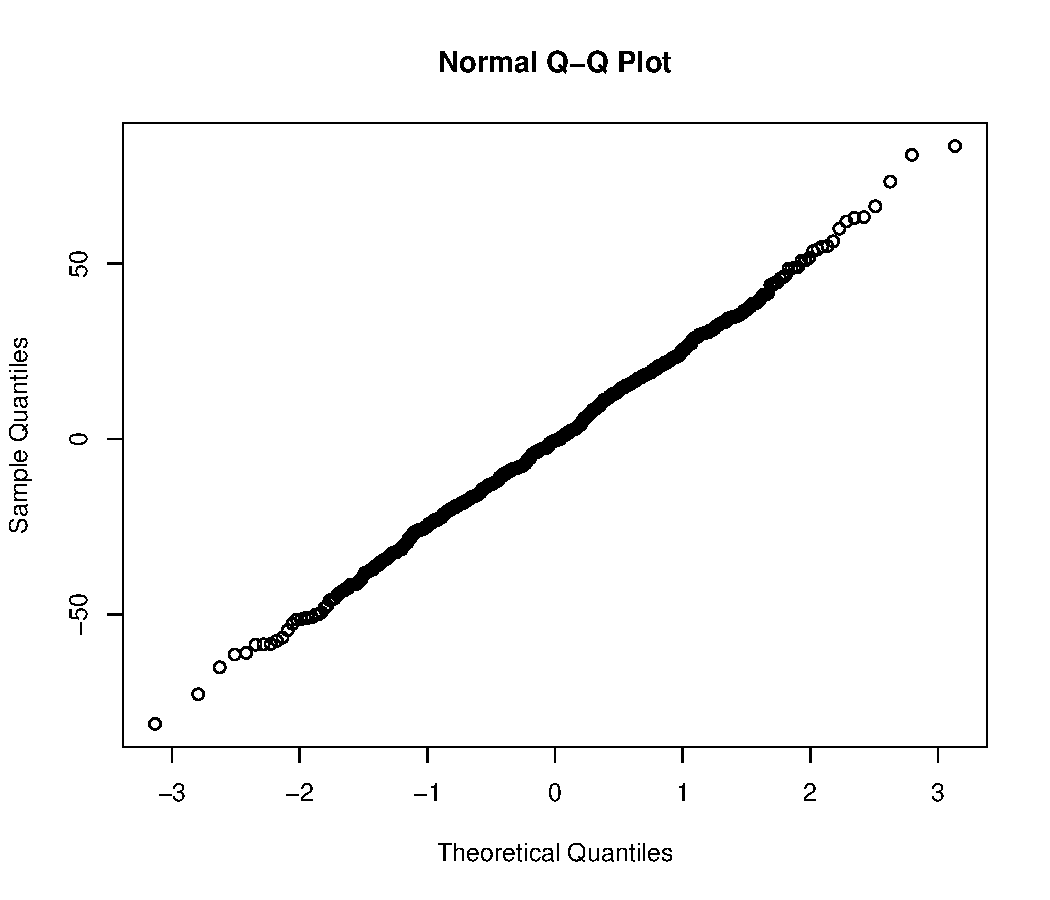
\includegraphics{03-Preliminaries_files/figure-latex/unnamed-chunk-20-1.pdf}

\hypertarget{variability}{%
\section{Variability}\label{variability}}

Researchers are critically interested in the spread or dispersion of the scores.

\hypertarget{range}{%
\subsection{Range}\label{range}}

The \textbf{range} is the simplest assessment of variability and is calculated by identifying the highest and lowest scores and subtracting the lowest from the highest. In our toy dataset, arranged from low-to-high (1, 2, 2, 3, 5 ) we see that the low is 1 and high is 5; 4 is the range. We can retrieve this data with three base R functions that ask for the minimum score, the maximum score, or both together -- the range:

\begin{Shaded}
\begin{Highlighting}[]
\FunctionTok{min}\NormalTok{(toy}\SpecialCharTok{$}\NormalTok{toy, }\AttributeTok{na.rm =} \ConstantTok{TRUE}\NormalTok{)}
\end{Highlighting}
\end{Shaded}

\begin{verbatim}
[1] 1
\end{verbatim}

\begin{Shaded}
\begin{Highlighting}[]
\FunctionTok{max}\NormalTok{(toy}\SpecialCharTok{$}\NormalTok{toy, }\AttributeTok{na.rm =} \ConstantTok{TRUE}\NormalTok{)}
\end{Highlighting}
\end{Shaded}

\begin{verbatim}
[1] 5
\end{verbatim}

\begin{Shaded}
\begin{Highlighting}[]
\FunctionTok{range}\NormalTok{(toy}\SpecialCharTok{$}\NormalTok{toy, }\AttributeTok{na.rm =} \ConstantTok{TRUE}\NormalTok{)}
\end{Highlighting}
\end{Shaded}

\begin{verbatim}
[1] 1 5
\end{verbatim}

The negative affect variable from our research vignette has the following range:

\begin{Shaded}
\begin{Highlighting}[]
\FunctionTok{min}\NormalTok{(df}\SpecialCharTok{$}\NormalTok{nAff)}
\end{Highlighting}
\end{Shaded}

\begin{verbatim}
[1] 1
\end{verbatim}

\begin{Shaded}
\begin{Highlighting}[]
\FunctionTok{max}\NormalTok{(df}\SpecialCharTok{$}\NormalTok{nAff)}
\end{Highlighting}
\end{Shaded}

\begin{verbatim}
[1] 4
\end{verbatim}

\begin{Shaded}
\begin{Highlighting}[]
\FunctionTok{range}\NormalTok{(df}\SpecialCharTok{$}\NormalTok{nAff)}
\end{Highlighting}
\end{Shaded}

\begin{verbatim}
[1] 1 4
\end{verbatim}

With a low of 1 and high of 4, the range of negative affect is 3. This is consistent with the description of the negative affect measure.

One limitation of the range is that it is easily influenced by extreme scores.

\hypertarget{percentiles-quantiles-interquartile-range}{%
\subsection{Percentiles, Quantiles, Interquartile Range}\label{percentiles-quantiles-interquartile-range}}

The \textbf{interquartile range} is middle 50\% of data, or the scores that fall between 25th and 75th percentiles. Before calculating that, let's first define \textbf{quantiles} and \textbf{percentiles}. \textbf{Quantiles} are values that split a data into equal portions. \textbf{Percentiles} divide the data into 100 equal parts. Percentiles are commonly used in testing and assessment. You may have encountered them in standardized tests such as the SAT and GRE where both the score obtained and its associated percentile are reported. When graduate programs evaluate GRE scores, depending on their criteria and degree of competitiveness they may set a threshold based on percentiles (e.g., using a cut of of the 50th, 75th, or higher percentile for the verbal or quantitative GRE scores).

We have already learned the value of the median. The median is also the 50th percentile. We can now use the \emph{quantile()} function and indicate we want the value at the 50\% percentile.

Let's first examine the toy dataset:

\begin{Shaded}
\begin{Highlighting}[]
\FunctionTok{median}\NormalTok{(toy}\SpecialCharTok{$}\NormalTok{toy, }\AttributeTok{na.rm =} \ConstantTok{TRUE}\NormalTok{)}
\end{Highlighting}
\end{Shaded}

\begin{verbatim}
[1] 2
\end{verbatim}

\begin{Shaded}
\begin{Highlighting}[]
\FunctionTok{quantile}\NormalTok{(toy}\SpecialCharTok{$}\NormalTok{toy, }\AttributeTok{probs =} \FloatTok{0.5}\NormalTok{, }\AttributeTok{na.rm =} \ConstantTok{TRUE}\NormalTok{)}
\end{Highlighting}
\end{Shaded}

\begin{verbatim}
50% 
  2 
\end{verbatim}

As shown by our calculation, the value at the median and the 50th percentile is 2.0. Let's look at those values for the research vignette:

\begin{Shaded}
\begin{Highlighting}[]
\FunctionTok{median}\NormalTok{(df}\SpecialCharTok{$}\NormalTok{nAff, }\AttributeTok{na.rm =} \ConstantTok{TRUE}\NormalTok{)}
\end{Highlighting}
\end{Shaded}

\begin{verbatim}
[1] 1.765367
\end{verbatim}

\begin{Shaded}
\begin{Highlighting}[]
\FunctionTok{quantile}\NormalTok{(df}\SpecialCharTok{$}\NormalTok{nAff, }\AttributeTok{probs =} \FloatTok{0.5}\NormalTok{, }\AttributeTok{na.rm =} \ConstantTok{TRUE}\NormalTok{)}
\end{Highlighting}
\end{Shaded}

\begin{verbatim}
     50% 
1.765367 
\end{verbatim}

Again, we see the same result. Half of the values for negative affect are below 1.76; half are above.

The \emph{quantile()} function is extremely useful. We can retrieve the raw score at any percentile, and we could ask for as many as we desired. Here's an example.

\begin{Shaded}
\begin{Highlighting}[]
\FunctionTok{quantile}\NormalTok{(df}\SpecialCharTok{$}\NormalTok{nAff, }\AttributeTok{probs =} \FunctionTok{c}\NormalTok{(}\FloatTok{0.1}\NormalTok{, }\FloatTok{0.2}\NormalTok{, }\FloatTok{0.3}\NormalTok{, }\FloatTok{0.4}\NormalTok{, }\FloatTok{0.5}\NormalTok{, }\FloatTok{0.6}\NormalTok{, }\FloatTok{0.7}\NormalTok{, }\FloatTok{0.8}\NormalTok{, }\FloatTok{0.9}\NormalTok{))}
\end{Highlighting}
\end{Shaded}

\begin{verbatim}
     10%      20%      30%      40%      50%      60%      70%      80% 
1.000000 1.142097 1.376633 1.582701 1.765367 1.943260 2.143177 2.360980 
     90% 
2.682303 
\end{verbatim}

\textbf{Quartiles} divide the data into four equal parts. The \textbf{interquartile range} is the spread of data between the 25th and 75th percentiles (or quartiles). We calculate the interquartile range by first obtaining those values, and then subtracting the lower from the higher.

\begin{Shaded}
\begin{Highlighting}[]
\FunctionTok{quantile}\NormalTok{(df}\SpecialCharTok{$}\NormalTok{nAff, }\AttributeTok{probs =} \FunctionTok{c}\NormalTok{(}\FloatTok{0.25}\NormalTok{, }\FloatTok{0.75}\NormalTok{))}
\end{Highlighting}
\end{Shaded}

\begin{verbatim}
     25%      75% 
1.271045 2.240372 
\end{verbatim}

We see that a score of 1.29 is at the 25th percentile and a score of 2.24 is at the 75th percentile. If we subtract 1.29 from 2.24\ldots{}

\begin{Shaded}
\begin{Highlighting}[]
\FloatTok{2.24} \SpecialCharTok{{-}} \FloatTok{1.29}
\end{Highlighting}
\end{Shaded}

\begin{verbatim}
[1] 0.95
\end{verbatim}

\ldots we learn that the interquartile range is 0.95. We could also obtain this value by using the \emph{IQR()} function in base R.

\begin{Shaded}
\begin{Highlighting}[]
\FunctionTok{IQR}\NormalTok{(df}\SpecialCharTok{$}\NormalTok{nAff, }\AttributeTok{na.rm =} \ConstantTok{TRUE}\NormalTok{)}
\end{Highlighting}
\end{Shaded}

\begin{verbatim}
[1] 0.9693262
\end{verbatim}

You may be asking, ``When would we use the interquartile range?'' When data are influenced by \textbf{outliers} (i.e., extreme scores), using a more truncated range (the middle 50\%, 75\%, 90\%) may be an option (if the dataset it large enough). At this point, though, the goal of this lesson is simply to introduce different ways of examining the variability in a dataset. Ultimately, we are working our way to the \textbf{standard deviation}. The next logical step is the \textbf{mean deviation.}

\hypertarget{deviations-around-the-mean}{%
\subsection{Deviations around the Mean}\label{deviations-around-the-mean}}

Nearly all statistics include assessments of variability in their calculation and most are based on deviations around the mean. In fact it might be good to pause for a moment and consider as the lessons in this OER (and those that follow) continue, we will be engaged in \emph{mathematical and statistical modeling}. In a featured article in the \emph{American Psychologist}, Rodgers \citeyearpar{rodgers_epistemology_2010} described models as a representation of reality that has two features:

\begin{itemize}
\tightlist
\item
  the model describes reality in some important ways, and
\item
  the model is simpler than reality.
\end{itemize}

Albeit one of the simplest, the mean is a statistical model. Rodgers noted this when he wrote, ``The mean and variance have done yeoman service to psychology and other behavioral sciences,'' \citeyearpar[p.~4]{rodgers_epistemology_2010}. These next statistical operations will walk through the use of the mean, particularly in its role in understanding variance. In later lessons, means and variances are used in understanding relations and differences.

A first step in understanding mean deviation is to ask, ``How far does each individual score deviates from the mean of scores?'' We can demonstrate this with our toy dataset. I am taking more steps than necessary to (a) make clear how the mean deviation (abbreviated, mdev) is calculated and (b) practice using R.

First, I will create a variable representing the mean:

\begin{Shaded}
\begin{Highlighting}[]
\CommentTok{\# Dissecting the script, each variable is referenced by}
\CommentTok{\# df\_nameDOLLARSIGNvariable\_name}
\NormalTok{toy}\SpecialCharTok{$}\NormalTok{mean }\OtherTok{\textless{}{-}} \FunctionTok{mean}\NormalTok{(toy}\SpecialCharTok{$}\NormalTok{toy, }\AttributeTok{na.rm =} \ConstantTok{TRUE}\NormalTok{)}
\FunctionTok{head}\NormalTok{(toy)  }\CommentTok{\#displays the first 6 rows of the data}
\end{Highlighting}
\end{Shaded}

\begin{verbatim}
  toy mean
1   2  2.6
2   3  2.6
3   2  2.6
4   1  2.6
5   5  2.6
6  NA  2.6
\end{verbatim}

Next, I will subtract the mean from each individual score. The result

\begin{Shaded}
\begin{Highlighting}[]
\NormalTok{toy}\SpecialCharTok{$}\NormalTok{mdev }\OtherTok{\textless{}{-}}\NormalTok{ toy}\SpecialCharTok{$}\NormalTok{toy }\SpecialCharTok{{-}}\NormalTok{ toy}\SpecialCharTok{$}\NormalTok{mean}
\FunctionTok{head}\NormalTok{(toy)  }\CommentTok{\#displays the first 6 rows of the data}
\end{Highlighting}
\end{Shaded}

\begin{verbatim}
  toy mean mdev
1   2  2.6 -0.6
2   3  2.6  0.4
3   2  2.6 -0.6
4   1  2.6 -1.6
5   5  2.6  2.4
6  NA  2.6   NA
\end{verbatim}

The variable, \emph{mdev} (short for ``mean deviation'') lets us know how far the individual score is from the mean. Unfortunately, it does not provide an overall estimate of variation. Further, summing and averaging these values all result in zero. Take a look:

\begin{Shaded}
\begin{Highlighting}[]
\CommentTok{\# Dissecting the script, Wrapping the sum and mean script in \textquotesingle{}round\textquotesingle{}}
\CommentTok{\# and following with the desired decimal places, provides a rounde}
\CommentTok{\# result.}
\FunctionTok{round}\NormalTok{(}\FunctionTok{sum}\NormalTok{(toy}\SpecialCharTok{$}\NormalTok{mdev, }\AttributeTok{na.rm =} \ConstantTok{TRUE}\NormalTok{), }\DecValTok{3}\NormalTok{)}
\end{Highlighting}
\end{Shaded}

\begin{verbatim}
[1] 0
\end{verbatim}

\begin{Shaded}
\begin{Highlighting}[]
\FunctionTok{round}\NormalTok{(}\FunctionTok{mean}\NormalTok{(toy}\SpecialCharTok{$}\NormalTok{mdev, }\AttributeTok{na.rm =} \ConstantTok{TRUE}\NormalTok{), }\DecValTok{3}\NormalTok{)}
\end{Highlighting}
\end{Shaded}

\begin{verbatim}
[1] 0
\end{verbatim}

One solution is to create the \emph{mean absolute deviation}. We first transform the mean deviation score to their absolute values, and then sum them.

\begin{Shaded}
\begin{Highlighting}[]
\NormalTok{toy}\SpecialCharTok{$}\NormalTok{abslt\_m }\OtherTok{\textless{}{-}} \FunctionTok{abs}\NormalTok{(toy}\SpecialCharTok{$}\NormalTok{mdev)}
\FunctionTok{head}\NormalTok{(toy)}
\end{Highlighting}
\end{Shaded}

\begin{verbatim}
  toy mean mdev abslt_m
1   2  2.6 -0.6     0.6
2   3  2.6  0.4     0.4
3   2  2.6 -0.6     0.6
4   1  2.6 -1.6     1.6
5   5  2.6  2.4     2.4
6  NA  2.6   NA      NA
\end{verbatim}

And now to average them:

\begin{Shaded}
\begin{Highlighting}[]
\FunctionTok{round}\NormalTok{(}\FunctionTok{mean}\NormalTok{(toy}\SpecialCharTok{$}\NormalTok{abslt\_m, }\AttributeTok{na.rm =} \ConstantTok{TRUE}\NormalTok{), }\DecValTok{3}\NormalTok{)}
\end{Highlighting}
\end{Shaded}

\begin{verbatim}
[1] 1.12
\end{verbatim}

This value tells how far individual observations are from the mean, ``on average.'' In our toy dataset, the average distance from the mean is 1.12.

So that we can keep statistical notation in our mind, this is the formula calculating the absolute mean deviation:

\[\sum_{i=1}^{n}|X_{i} - \bar{X}|\] Let's quickly repeat the process with the negative affect variable in our research vignette. So that we can more clearly see the relationship of the new variables to negative affect, let me create a df containing only nAff:

\begin{Shaded}
\begin{Highlighting}[]
\FunctionTok{library}\NormalTok{(tidyverse)}
\NormalTok{df\_nAff }\OtherTok{\textless{}{-}}\NormalTok{ df }\SpecialCharTok{\%\textgreater{}\%}
\NormalTok{    dplyr}\SpecialCharTok{::}\FunctionTok{select}\NormalTok{(nAff)}
\end{Highlighting}
\end{Shaded}

\begin{Shaded}
\begin{Highlighting}[]
\NormalTok{df\_nAff}\SpecialCharTok{$}\NormalTok{mdevNA }\OtherTok{\textless{}{-}}\NormalTok{ df\_nAff}\SpecialCharTok{$}\NormalTok{nAff }\SpecialCharTok{{-}} \FunctionTok{mean}\NormalTok{(df\_nAff}\SpecialCharTok{$}\NormalTok{nAff, }\AttributeTok{na.rm =} \ConstantTok{TRUE}\NormalTok{)}
\NormalTok{df\_nAff}\SpecialCharTok{$}\NormalTok{abNAmdev }\OtherTok{\textless{}{-}} \FunctionTok{abs}\NormalTok{(df\_nAff}\SpecialCharTok{$}\NormalTok{mdevNA)}
\FunctionTok{head}\NormalTok{(df\_nAff)}
\end{Highlighting}
\end{Shaded}

\begin{verbatim}
      nAff     mdevNA  abNAmdev
1 1.109882 -0.7038658 0.7038658
2 1.000000 -0.8137481 0.8137481
3 1.075573 -0.7381750 0.7381750
4 1.000000 -0.8137481 0.8137481
5 1.025246 -0.7885020 0.7885020
6 1.920559  0.1068111 0.1068111
\end{verbatim}

\begin{Shaded}
\begin{Highlighting}[]
\FunctionTok{round}\NormalTok{(}\FunctionTok{mean}\NormalTok{(df\_nAff}\SpecialCharTok{$}\NormalTok{abNAmdev, }\AttributeTok{na.rm =} \ConstantTok{TRUE}\NormalTok{), }\DecValTok{3}\NormalTok{)}
\end{Highlighting}
\end{Shaded}

\begin{verbatim}
[1] 0.523
\end{verbatim}

Thus, the absolute mean deviation for the negative affect variable in our research vignette is 0.521.

Although relatively intuitive, the absolute mean deviation is not all that useful. Most statistics texts include it because it is one of the steps toward variance, and ultimately, the standard deviation.

\hypertarget{variance}{%
\subsection{Variance}\label{variance}}

Variance is considered to be an \emph{average} dispersion calculated by summing the squared deviations and dividing by the number of observations (minus 1; more on that in later lessons).

Our next step is to square the mean deviations. This value is also called the \emph{sum of squared errors}, \emph{sum of squared deviations around the mean}, or \emph{sums of squares} and is abbreviated as \emph{SS}. Below are common statistical representations:

\[SS = \sum_{i=1}^{n}(X_{i} - \bar{X})^{^{2}}\] Let's do it with our toy data.

\begin{Shaded}
\begin{Highlighting}[]
\NormalTok{toy}\SpecialCharTok{$}\NormalTok{mdev2 }\OtherTok{\textless{}{-}}\NormalTok{ (toy}\SpecialCharTok{$}\NormalTok{mdev) }\SpecialCharTok{*}\NormalTok{ (toy}\SpecialCharTok{$}\NormalTok{mdev)}
\FunctionTok{sum}\NormalTok{(toy}\SpecialCharTok{$}\NormalTok{mdev2, }\AttributeTok{na.rm =} \ConstantTok{TRUE}\NormalTok{)  }\CommentTok{\#sum of squared deviations}
\end{Highlighting}
\end{Shaded}

\begin{verbatim}
[1] 9.2
\end{verbatim}

\begin{Shaded}
\begin{Highlighting}[]
\FunctionTok{head}\NormalTok{(toy)}
\end{Highlighting}
\end{Shaded}

\begin{verbatim}
  toy mean mdev abslt_m mdev2
1   2  2.6 -0.6     0.6  0.36
2   3  2.6  0.4     0.4  0.16
3   2  2.6 -0.6     0.6  0.36
4   1  2.6 -1.6     1.6  2.56
5   5  2.6  2.4     2.4  5.76
6  NA  2.6   NA      NA    NA
\end{verbatim}

Thus, our \emph{SS} (sums of squares or sums of squared errors) is 9.2.

To obtain the variance we divide by \emph{N} (or \emph{N} - 1; described in later lessons). Here are the updated formulas:

\[s^{2}=\frac{SS}{N-1}=\frac{\sum_{i=1}^{n}(X_{i} - \bar{X})^{^{2}}}{N-1}\] Let's do this with the toy data:

\begin{Shaded}
\begin{Highlighting}[]
\FloatTok{9.2}\SpecialCharTok{/}\NormalTok{(}\DecValTok{5} \SpecialCharTok{{-}} \DecValTok{1}\NormalTok{)  }\CommentTok{\#calculated with the previously obtained values}
\end{Highlighting}
\end{Shaded}

\begin{verbatim}
[1] 2.3
\end{verbatim}

\begin{Shaded}
\begin{Highlighting}[]
\CommentTok{\# to obtain the \textquotesingle{}correct\textquotesingle{} calculation by using each of these}
\CommentTok{\# individual R commands, we need to have non{-}missing data}
\NormalTok{toy }\OtherTok{\textless{}{-}} \FunctionTok{na.omit}\NormalTok{(toy)}
\FunctionTok{sum}\NormalTok{(toy}\SpecialCharTok{$}\NormalTok{mdev2, }\AttributeTok{na.rm =} \ConstantTok{TRUE}\NormalTok{)}\SpecialCharTok{/}\NormalTok{((}\FunctionTok{nrow}\NormalTok{(toy) }\SpecialCharTok{{-}} \DecValTok{1}\NormalTok{))  }\CommentTok{\#variance}
\end{Highlighting}
\end{Shaded}

\begin{verbatim}
[1] 2.3
\end{verbatim}

Of course R also has a function that will do all the steps for us:

\begin{Shaded}
\begin{Highlighting}[]
\FunctionTok{mean}\NormalTok{(toy}\SpecialCharTok{$}\NormalTok{toy, }\AttributeTok{na.rm =} \ConstantTok{TRUE}\NormalTok{)}
\end{Highlighting}
\end{Shaded}

\begin{verbatim}
[1] 2.6
\end{verbatim}

\begin{Shaded}
\begin{Highlighting}[]
\FunctionTok{var}\NormalTok{(toy}\SpecialCharTok{$}\NormalTok{toy, }\AttributeTok{na.rm =} \ConstantTok{TRUE}\NormalTok{)}
\end{Highlighting}
\end{Shaded}

\begin{verbatim}
[1] 2.3
\end{verbatim}

The variance around the mean (2.6) of our toy data is 2.3.

Let's quickly repeat this process with the negative affect variable from the research vignette. In prior steps we had calculated the mean deviations by subtracting the mean from each individual score. Next we square the mean deviations\ldots.

\begin{Shaded}
\begin{Highlighting}[]
\NormalTok{df\_nAff}\SpecialCharTok{$}\NormalTok{NAmd2 }\OtherTok{\textless{}{-}}\NormalTok{ (df\_nAff}\SpecialCharTok{$}\NormalTok{mdevNA) }\SpecialCharTok{*}\NormalTok{ (df\_nAff}\SpecialCharTok{$}\NormalTok{mdevNA)}
\FunctionTok{head}\NormalTok{(df\_nAff)}
\end{Highlighting}
\end{Shaded}

\begin{verbatim}
      nAff     mdevNA  abNAmdev      NAmd2
1 1.109882 -0.7038658 0.7038658 0.49542700
2 1.000000 -0.8137481 0.8137481 0.66218597
3 1.075573 -0.7381750 0.7381750 0.54490233
4 1.000000 -0.8137481 0.8137481 0.66218597
5 1.025246 -0.7885020 0.7885020 0.62173547
6 1.920559  0.1068111 0.1068111 0.01140861
\end{verbatim}

\ldots{} and sum them.

\begin{Shaded}
\begin{Highlighting}[]
\FunctionTok{sum}\NormalTok{(df\_nAff}\SpecialCharTok{$}\NormalTok{NAmd2, }\AttributeTok{na.rm =} \ConstantTok{TRUE}\NormalTok{)  }\CommentTok{\#sum of squared deviations}
\end{Highlighting}
\end{Shaded}

\begin{verbatim}
[1] 283.8923
\end{verbatim}

Our sums of squared deviations around the mean is 283.44. When we divide it by \emph{N} - 1, we obtain the variance. We can check our work with (a) the values we calculated at each step, (b) the steps written in separate R code, and (c) the \emph{var()} function.

\begin{Shaded}
\begin{Highlighting}[]
\FloatTok{283.44}\SpecialCharTok{/}\NormalTok{(}\DecValTok{713} \SpecialCharTok{{-}} \DecValTok{1}\NormalTok{)  }\CommentTok{\# calculating with the individual pre{-}calculated values}
\end{Highlighting}
\end{Shaded}

\begin{verbatim}
[1] 0.3980899
\end{verbatim}

\begin{Shaded}
\begin{Highlighting}[]
\FunctionTok{sum}\NormalTok{(df\_nAff}\SpecialCharTok{$}\NormalTok{NAmd2, }\AttributeTok{na.rm =} \ConstantTok{TRUE}\NormalTok{)}\SpecialCharTok{/}\NormalTok{((}\FunctionTok{nrow}\NormalTok{(df\_nAff) }\SpecialCharTok{{-}} \DecValTok{1}\NormalTok{))  }\CommentTok{\#calculated with steps from separate R code}
\end{Highlighting}
\end{Shaded}

\begin{verbatim}
[1] 0.3987252
\end{verbatim}

\begin{Shaded}
\begin{Highlighting}[]
\FunctionTok{var}\NormalTok{(df\_nAff}\SpecialCharTok{$}\NormalTok{nAff)  }\CommentTok{\#calculated using the base R function}
\end{Highlighting}
\end{Shaded}

\begin{verbatim}
[1] 0.3987252
\end{verbatim}

Unfortunately, because the mean deviations were squared, this doesn't interpret well. Hence, we move to the \emph{standard deviation}.

\hypertarget{standard-deviation}{%
\subsection{Standard Deviation}\label{standard-deviation}}

The standard deviation is simply the square root of the variance. Stated another way, it is an estimate of the average spread of data, presented in the same metric as the data.

Calculating the standard deviation requires earlier steps:

\begin{enumerate}
\def\labelenumi{\arabic{enumi}.}
\tightlist
\item
  Calculating the mean.
\item
  Calculating mean deviations by subtracting the mean from each individual score.
\item
  Squaring the mean deviations.
\item
  Summing the mean deviations to create the \emph{SS}, or sums of squares.
\item
  Dividing the \emph{SS} by \emph{N} - 1; this results in the \emph{variance} around the mean.
\end{enumerate}

The 6th step is to take the square root of variance. It is represented in the formula, below:

\[s=\sqrt{\frac{SS}{N-1}}=\sqrt{\frac{\sum_{i=1}^{n}(X_{i} - \bar{X})^{^{2}}}{N-1}}\] Repeated below are each of the six steps for the toy data:

\begin{Shaded}
\begin{Highlighting}[]
\CommentTok{\# six steps wrapped into 1}
\NormalTok{toy}\SpecialCharTok{$}\NormalTok{mdev }\OtherTok{\textless{}{-}}\NormalTok{ toy}\SpecialCharTok{$}\NormalTok{toy }\SpecialCharTok{{-}} \FunctionTok{mean}\NormalTok{(toy}\SpecialCharTok{$}\NormalTok{toy, }\AttributeTok{na.rm =} \ConstantTok{TRUE}\NormalTok{)}
\NormalTok{toy}\SpecialCharTok{$}\NormalTok{mdev2 }\OtherTok{\textless{}{-}}\NormalTok{ (toy}\SpecialCharTok{$}\NormalTok{mdev) }\SpecialCharTok{*}\NormalTok{ (toy}\SpecialCharTok{$}\NormalTok{mdev)}
\CommentTok{\# I can save the variance calculation as an object for later use}
\NormalTok{toy\_var }\OtherTok{\textless{}{-}} \FunctionTok{sum}\NormalTok{(toy}\SpecialCharTok{$}\NormalTok{mdev2)}\SpecialCharTok{/}\NormalTok{(}\FunctionTok{nrow}\NormalTok{(toy) }\SpecialCharTok{{-}} \DecValTok{1}\NormalTok{)}
\CommentTok{\# checking work with the variance function}
\FunctionTok{var}\NormalTok{(toy}\SpecialCharTok{$}\NormalTok{toy)}
\end{Highlighting}
\end{Shaded}

\begin{verbatim}
[1] 2.3
\end{verbatim}

The seventh step is to take the square root of variance.

\begin{Shaded}
\begin{Highlighting}[]
\CommentTok{\# grabbing the mean for quick reference}
\FunctionTok{mean}\NormalTok{(toy}\SpecialCharTok{$}\NormalTok{toy)}
\end{Highlighting}
\end{Shaded}

\begin{verbatim}
[1] 2.6
\end{verbatim}

\begin{Shaded}
\begin{Highlighting}[]
\CommentTok{\# below the \textquotesingle{}toy\_var\textquotesingle{} object was created in the prior step}
\FunctionTok{sqrt}\NormalTok{(toy\_var)}
\end{Highlighting}
\end{Shaded}

\begin{verbatim}
[1] 1.516575
\end{verbatim}

\begin{Shaded}
\begin{Highlighting}[]
\CommentTok{\# checking work with the R function to calculate standard deviation}
\FunctionTok{sd}\NormalTok{(toy}\SpecialCharTok{$}\NormalTok{toy)}
\end{Highlighting}
\end{Shaded}

\begin{verbatim}
[1] 1.516575
\end{verbatim}

It is common to report means and standard deviations for continuous variables in our datasets. For the toy data our mean is 2.6 with a standard deviation of 1.52.

Let's repeat the process for the negative affect variable in the research vignette. First the six steps to calculate variance.

\begin{Shaded}
\begin{Highlighting}[]
\CommentTok{\# six steps wrapped into 1}
\NormalTok{df\_nAff}\SpecialCharTok{$}\NormalTok{mdevNA }\OtherTok{\textless{}{-}}\NormalTok{ df\_nAff}\SpecialCharTok{$}\NormalTok{nAff }\SpecialCharTok{{-}} \FunctionTok{mean}\NormalTok{(df\_nAff}\SpecialCharTok{$}\NormalTok{nAff, }\AttributeTok{na.rm =} \ConstantTok{TRUE}\NormalTok{)}
\NormalTok{df\_nAff}\SpecialCharTok{$}\NormalTok{NAmd2 }\OtherTok{\textless{}{-}}\NormalTok{ (df\_nAff}\SpecialCharTok{$}\NormalTok{mdevNA) }\SpecialCharTok{*}\NormalTok{ (df\_nAff}\SpecialCharTok{$}\NormalTok{mdevNA)}
\CommentTok{\# I can save the variance calculation as an object for later use}
\NormalTok{nAff\_var }\OtherTok{\textless{}{-}} \FunctionTok{sum}\NormalTok{(df\_nAff}\SpecialCharTok{$}\NormalTok{NAmd2)}\SpecialCharTok{/}\NormalTok{(}\FunctionTok{nrow}\NormalTok{(df) }\SpecialCharTok{{-}} \DecValTok{1}\NormalTok{)}
\CommentTok{\# checking work with the variance function}
\FunctionTok{var}\NormalTok{(df\_nAff}\SpecialCharTok{$}\NormalTok{nAff)}
\end{Highlighting}
\end{Shaded}

\begin{verbatim}
[1] 0.3987252
\end{verbatim}

The seventh step is to take the square root of variance.

\begin{Shaded}
\begin{Highlighting}[]
\CommentTok{\# grabbing the mean for quick reference}
\FunctionTok{mean}\NormalTok{(df\_nAff}\SpecialCharTok{$}\NormalTok{nAff)}
\end{Highlighting}
\end{Shaded}

\begin{verbatim}
[1] 1.813748
\end{verbatim}

\begin{Shaded}
\begin{Highlighting}[]
\CommentTok{\# below the \textquotesingle{}toy\_var\textquotesingle{} object was created in the prior step}
\FunctionTok{sqrt}\NormalTok{(nAff\_var)}
\end{Highlighting}
\end{Shaded}

\begin{verbatim}
[1] 0.6314469
\end{verbatim}

\begin{Shaded}
\begin{Highlighting}[]
\CommentTok{\# checking work with the R function to calculate standard deviation}
\FunctionTok{sd}\NormalTok{(df\_nAff}\SpecialCharTok{$}\NormalTok{nAff)}
\end{Highlighting}
\end{Shaded}

\begin{verbatim}
[1] 0.6314469
\end{verbatim}

In APA Style we use \emph{M} and \emph{SD} as abbreviations for mean and standard deviation, respectively. In APA Style, non-Greek statistical symbols such as these are italicized. Thus we would write \emph{M} = 1.81(\emph{SD} = 0.63) in a statistical string of results.

We can examine the standard deviation in relation to its mean to understand how narrowly or broadly the data is distributed. Relative to a same-sized mean, a small standard deviation means that the mean represents the data well. A larger standard deviation, conveys that there is greater variability and the mean, alone, is a less valid representation of the score.

In later lessons we will explore the standard deviation in more detail -- learning how we can use it in the determination of the significance and magnitude of relations and differences.

\hypertarget{are-the-variables-normally-distributed}{%
\section{Are the Variables Normally Distributed?}\label{are-the-variables-normally-distributed}}

Statistics that we use are accompanied by assumptions about the nature of variables in the dataset. A common assumption is that the data are \emph{normally distributed}. That is, the data presumes a standard normal curve.

For a streamlined presentation, let me create a df with three, continuously scaled, variables of interest.

\begin{Shaded}
\begin{Highlighting}[]
\CommentTok{\# I have opened the tidyverse library so that I can use the pipe}
\FunctionTok{library}\NormalTok{(tidyverse)}
\NormalTok{df\_3vars }\OtherTok{\textless{}{-}}\NormalTok{ df }\SpecialCharTok{\%\textgreater{}\%}
\NormalTok{    dplyr}\SpecialCharTok{::}\FunctionTok{select}\NormalTok{(nAff, mAggr, drProb)}
\end{Highlighting}
\end{Shaded}

\hypertarget{skew-and-kurtosis}{%
\subsection{Skew and Kurtosis}\label{skew-and-kurtosis}}

Skew and kurtosis are indicators of non-normality. Skew refers to the degree to which the data is symmetrical. In the figure below, the symmetrical distribution in the center (the black line) has no apparent evidence of skew. In contrast, the red figure whose curve (representing a majority of observations) in the left-most part of the graph (with the tail pulling to the right) is positively skewed; the blue figure whose curve (representing a majority of cases) is in the right-most part of the graph (with the tail pulling to the left) is negatively skewed.

\includegraphics{03-Preliminaries_files/figure-latex/unnamed-chunk-48-1.pdf} Kurtosis refers to the degree to which the distribution of data is flat or peaked. Mesokurtic distributions are considered to be closest to normal. Leptokurtic distributions are peaked and platykurtic distributions are flat. As we will learn as we progress, visual observation of data is a legitimate component in evaluating skew and kurtosis.

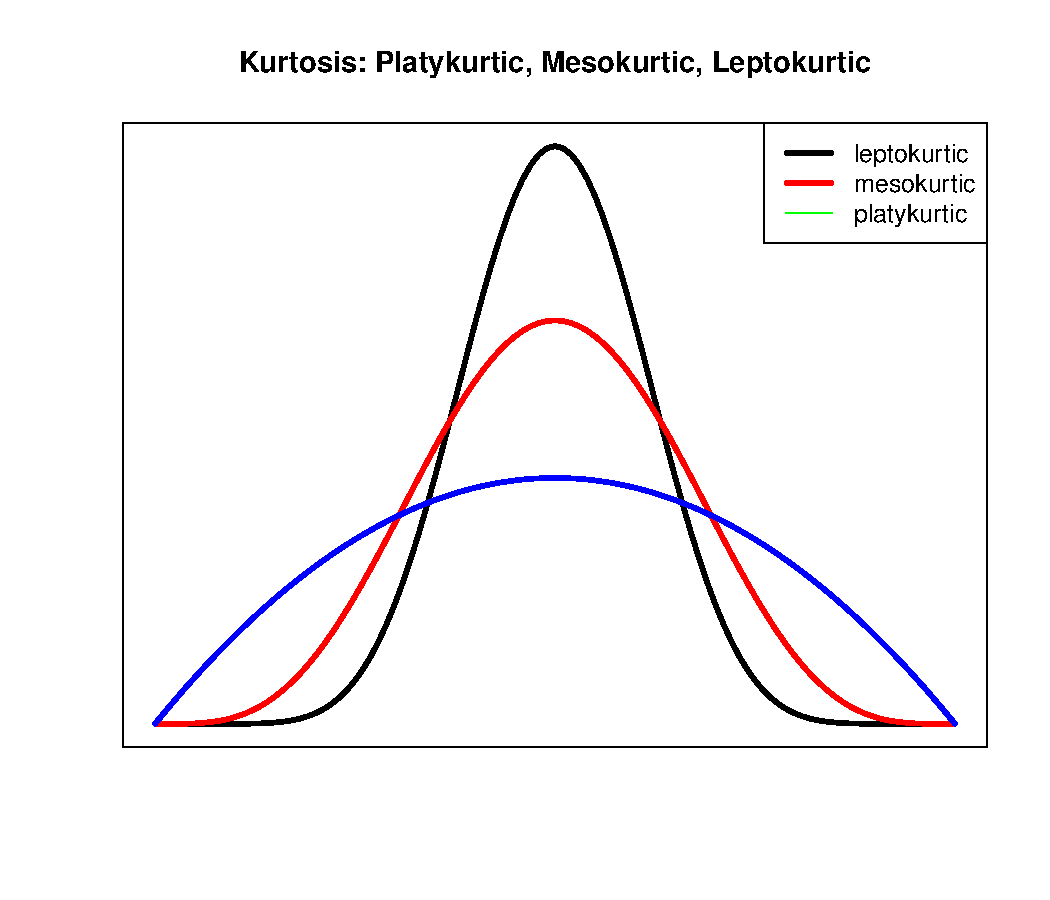
\includegraphics{03-Preliminaries_files/figure-latex/unnamed-chunk-49-1.pdf} There have been numerous approaches to calculating and interpreting skew and kurtosis. Consequently, different statistics packages calculate skew and kurtosis differently. The \emph{psych} package (a go-to-for a variety of tasks) offers three different options for calculating skew and kurtosis. These are specified in the script as ``type=\#'' (i.e., 1, 2, or 3 {[}the default{]}). Revelle \citeyearpar{revelle_introduction_2021} refers readers to Joanes and Gill's \citeyearpar{joanes_comparing_1998} article for detailed information about each. A very helpful resource to understand skew, kurtosis, and its interpretation is found in chapter four (Data Preparation and Psychometrics Review) of Kline's \citeyearpar{kline_data_2016} SEM text is helpful in the interpretation of skew and kurtosis. Summarizing by simulation studies for structural equation modeling (i.e., multivariate statistics that are generally characterized as large sample studies using maximum likelihood estimation), Kline suggested that \emph{type=1} skew values greater than the absolute value of 3.0 are ``severely'' skewed. Regarding \emph{type=1} kurtosis, Kline noted the literature has suggested that values from 8.0 to 20.0 have been described as severely kurtotic. As an interpretive framework, Kline suggested that absolute values greater than 10.0 are problematic and values greater than 20 are serious. He added that this rule-of-thumb errs on the conservative side.

The \emph{psych::describe} specification of ``type=1'' results in the \emph{skew index} and \emph{kurtosis index}. For simplicity sake, I will refer to this specific variation of skew and kutosis as ``type=1.'' This is a very quick way to obtain initial values.

\begin{Shaded}
\begin{Highlighting}[]
\NormalTok{psych}\SpecialCharTok{::}\FunctionTok{describe}\NormalTok{(df\_3vars, }\AttributeTok{type =} \DecValTok{1}\NormalTok{)}
\end{Highlighting}
\end{Shaded}

\begin{verbatim}
       vars   n mean   sd median trimmed  mad min   max range skew kurtosis
nAff      1 713 1.81 0.63   1.77    1.76 0.72   1  4.00  3.00 0.51    -0.42
mAggr     2 713 2.49 2.19   2.17    2.24 2.43   0 11.42 11.42 0.91     0.65
drProb    3 713 2.92 2.78   2.33    2.58 3.45   0 11.90 11.90 0.78    -0.21
         se
nAff   0.02
mAggr  0.08
drProb 0.10
\end{verbatim}

Using Kline's \citeyearpar{kline_data_2016} guidelines for evaluation, a quick review of the type=1 output indicates that no skew value exceeded the absolute value of 3.0. That is, across the nAff, mAggr, and drProb variables the highest type=1 skew value was 0.93 Regarding kurtosis, no value had a greater magnitude then .59 and all fell below the absolute value of 10. A limitation of the type=1 output and Kline's interpretative guidelines is that the simulation studies that led to the interpretive guidelines were based on structural equation modeling. These statistics are multivariate in nature, they typically use maximum likelihood estimators, and are based on large samples.

An alternative tool for identifying distributions that are severely skewed or kurtotic is the ``skew.2SE'' and ``kurt.2SE'' output from \emph{pastecs::stat.desc}.

These values represent the type=1 skew (or kurtosis) value divided by two-times its respective standard error (i.e., the standard error of the skew or kurtosis distribution, not the \emph{se} value associated with the variable). The result is a standardized value that, on its own, indicates statistical significance. In the case of skew.2SE and kurt2SE, values of 1 (\emph{p} \textless{} .05), 1.29 (\emph{p} \textless{} .01), and 1.65 (\emph{p} \textless{} .001) represent statistically significant departures from symmetry (skew) and normal peakedness (kurtosis). Unfortunately, this tool is not without criticism.

\(skew.2SE = \frac{S-0}{2*SE_{skewness}}\) and \(kurt.2SE = \frac{S-0}{2*SE_{kurtosis}}\)

The skew.2SE and kurt.2SE values can be obtained with \emph{pastecs::stat.desc} by adding the ``norm = TRUE'' statement.

\begin{Shaded}
\begin{Highlighting}[]
\NormalTok{pastecs}\SpecialCharTok{::}\FunctionTok{stat.desc}\NormalTok{(df\_3vars, }\AttributeTok{norm =} \ConstantTok{TRUE}\NormalTok{)}
\end{Highlighting}
\end{Shaded}

\begin{verbatim}
                                   nAff                          mAggr
nbr.val       713.000000000000000000000  713.0000000000000000000000000
nbr.null        0.000000000000000000000  119.0000000000000000000000000
nbr.na          0.000000000000000000000    0.0000000000000000000000000
min             1.000000000000000000000    0.0000000000000000000000000
max             4.000000000000000000000   11.4193472349555946721011424
range           3.000000000000000000000   11.4193472349555946721011424
sum          1293.202396986186386129702 1772.9047547268992275348864496
median          1.765366956719584212721    2.1702325413588932079278493
mean            1.813748102364917569318    2.4865424329970533534606147
SE.mean         0.023647871456839660714    0.0821091579065054283370628
CI.mean.0.95    0.046427899159900143378    0.1612050247458937379807509
var             0.398725160825158186917    4.8069845480383115443601127
std.dev         0.631446878862472638083    2.1924836482943974580450686
coef.var        0.348144749559841870656    0.8817398887706798804586583
skewness        0.509847355388718947999    0.9072670817943200294308781
skew.2SE        2.784775604496556589140    4.9554738480840363479273947
kurtosis       -0.431370013354644310510    0.6446009591154999718298768
kurt.2SE       -1.179701916057711574837    1.7628415583352385898052717
normtest.W      0.947747894960071946002    0.9160358300310357249074400
normtest.p      0.000000000000003548014    0.0000000000000000001931087
                                       drProb
nbr.val       713.000000000000000000000000000
nbr.null      176.000000000000000000000000000
nbr.na          0.000000000000000000000000000
min             0.000000000000000000000000000
max            11.897269669625760712960982346
range          11.897269669625760712960982346
sum          2080.674335793011778150685131550
median          2.327140791884834580827146056
mean            2.918196824394125865609339598
SE.mean         0.104209937080375208973137546
CI.mean.0.95    0.204595515459292442983496585
var             7.742973933228878280488061137
std.dev         2.782619976430284580715124321
coef.var        0.953540882907379039323814141
skewness        0.777725776691186476696771024
skew.2SE        4.247921945709623336995264253
kurtosis       -0.215619970410508177138808605
kurt.2SE       -0.589673098172587506482500430
normtest.W      0.898257151085984140159723665
normtest.p      0.000000000000000000002486005
\end{verbatim}

Statisticians have noted that these standardized values are quite sensitive to sample size \citep{field_discovering_2012, kline_data_2016}. In large samples even minor deviations from normality may appear as statistically significant. In contrast, small samples with lower power may be severely non-normal, but skew and kurtosis could go undetected. When sample sizes are smaller, using the 1.96 (or ``2'') criteria is acceptable in determining a significant skew or kurtosis, however, as the sample size increases, the probability of rejecting the hypothesis that skew (or kurtosis) also zero increases. Field \citeyearpar{field_discovering_2012} noted that in such cases it is appropriate to relax the standard and evaluate skew or kurtosis against the 1.29 (\emph{p} \textless{} .01) criteria. Further, when samples are larger than 200, it may be more appropriate to abandon the interpretation of the \emph{z}-values and, instead, examine the shape of the distribution rather than to interpret these standardized values.

Comparing the skewness and kurtosis type=1 values to the skew.2SE and kurt.2SE values, we can see the interpretive challenges.

\begin{longtable}[]{@{}lcccc@{}}
\toprule\noalign{}
Variable & skewness & skew.2SE & kurtosis & kurt.2SE \\
\midrule\noalign{}
\endhead
\bottomrule\noalign{}
\endlastfoot
nAff & 0.575 & 3.141*** & -0.176 & -0.481 \\
mAggr & 0.926 & 5.059*** & 0.575 & 1.572** \\
drProb & 0.783 & 4.278*** & -0.168 & -0.460 \\
\end{longtable}

Values in the ``skewness'' column are concerning when they are exceed the absolute value of 3.0; none are. Values in the ``skew.2SE'' column are statistically significant at \(p < .001\) when they exceed 1.65. Here, the two approaches to interpreting skew both suggest positive skew (i.e., heavy distribution in the left with a long tail to the right), but only the ``skew.2SE'' results suggest that the degree of skewness is significant/concerning.

Regarding kurtosis, values in the ``kurtosis'' column become concerning when they exceed the absolute value of 10; none are. Values in the ``kurt.2SE'' become statistically significant when they exceed 1.0. The mAggr variable's value of 1.572 is statistically significant at \(p < .01\).

So how do we think about skewness and kurtosis in our data? First, I simulated a dataset with more than 700 cases. This far exceeds the ``large'' sample size of 200. Therefore, interpreting the type 1 skewness and kurtosis values according to Kline's \citeyearpar{kline_data_2016} criteria of less than the absolute values of 3 and 10, respectively, is probably most appropriate. Further, skewness and kurtosis are only two dimensions of assessing whether or not a distribution is normally distributed. Thus, I will keep these results in mind as I examine additional metrics (especially when we look at histograms with superimposed curve).

In this OER, I will predominantly use the type=1 output from the \emph{psych::describe} package and use Kline's \citeyearpar{kline_data_2016} interpretive criteria. I do think the ``skew.2SE'' and ``kurt.2SE'' metrics can be useful when sample sizes are smaller (perhaps \(N = 100\) or less) and ordinary least squares (such as used in ANOVA and regression models) statistics will be utilized. In any case, if I have significant concerns about normality, I always return to more extensive and authoritative sources to make my decisions about preparing my data for analysis.

\hypertarget{shapiro-wilk-test-of-normality}{%
\subsection{Shapiro-Wilk Test of Normality}\label{shapiro-wilk-test-of-normality}}

In addition to skew and kurtosis, there are formal statistical tests that evaluate whether or not our data is statistically significantly different than a normal distribution. One of those is the Shapiro-Wilk test of normality. The output we obtained from \emph{pastecs::stat.desc} included the Shapiro-Wilk test value and the associated \emph{p} value. When \(p < .05\), our data is statistically significantly different from a normal distribution.

In our simulated data, all variables were statistically significantly different than a normal distribution (\(nAff: W = 0.948, p < .001; mAggr: W = 0.913, p < .001; drProb: W = 0.900, p < .001\)).

Just because data is skewed, kurtotic, or non-normally distributed does not (necessarily) mean that we cannot use it. As we move through the lessons in this OER we will evaluate the quality of the data according to the statistical assumptions associated with the statistic we are using. Often there are tools that we can use (e.g., variations of the statistic that are robust to violations of assumptions, deleting univariate or multivariate outliers) in spite of our data characteristics.

\hypertarget{relations-between-variables}{%
\section{Relations between Variables}\label{relations-between-variables}}

Preliminary investigation of data almost always includes a report of their bivariate relations. Correlation coefficients express the magnitude of relationships on a scale ranging from -1 to +1. A correlation coefficient of

\begin{itemize}
\tightlist
\item
  -1.0 implies a 1:1 inverse relationship, such that for every unit of increase in variable A, there is a similar decrease in variable B,
\item
  0.0 implies no correspondence between two variables,
\item
  1.0 implies that as A increases by one unit, so does B.
\end{itemize}

Correlation coefficients are commonly represented in two formulas. In a manner that echoes the calculation of \emph{variance}, the first part of the calculation estimates the covariation (i.e., \emph{covariance}) of the two variables of interest.

\[
\mbox{Cov}(X,Y) = \frac{1}{N-1} \sum_{i=1}^N \left( X_i - \bar{X} \right) \left( Y_i - \bar{Y} \right)
\]

The problem is that the result is unstandardized and difficult to interpret. Therefore, the second part of the calculation of the correlation coefficient results in the standardization of the metric in the -1 to +1 scale. \[
r_{XY}  = \frac{\mbox{Cov}(X,Y)}{ \hat{\sigma}_X \ \hat{\sigma}_Y}
\] Covariation and correlation matrices are central to many of our statistics therefore, those of who teach statistics believe that it is important to take a look ``under the hood.'' From our research vignette, let's calculate the relationship between negative affect and psychological distress.

Examining the first formula, some parts should look familiar:

\begin{itemize}
\tightlist
\item
  \((X_i - \bar{X})\): We can see that we need to subtract the mean from the first(X) variable in involved in the correlation; we saw this when we calculated \emph{mean deviations}.
\item
  \((Y_i - \bar{Y})\): We repeat the \emph{mean deviation} process for the second (Y) variable.
\end{itemize}

Let's work step-by-step through the calculation of a correlation coefficient. So that we can more easily see what we are doing with the variables, I will create a super tiny dataframe with the two variables of interest (negative affect and microaggressions):

\begin{Shaded}
\begin{Highlighting}[]
\CommentTok{\# just in case it turned off, I\textquotesingle{}m reopening tidyverse so that I can}
\CommentTok{\# use the pipe}
\FunctionTok{library}\NormalTok{(tidyverse)}
\CommentTok{\# using the dplyr package to select the two variables in this tiny df}
\NormalTok{df4corr }\OtherTok{\textless{}{-}}\NormalTok{ df }\SpecialCharTok{\%\textgreater{}\%}
\NormalTok{    dplyr}\SpecialCharTok{::}\FunctionTok{select}\NormalTok{(nAff, mAggr)}
\CommentTok{\# displaying the first 6 rows of df4corr (\textquotesingle{}dataframe for}
\CommentTok{\# correlations\textquotesingle{} {-}{-} I made this up)}
\FunctionTok{head}\NormalTok{(df4corr)}
\end{Highlighting}
\end{Shaded}

\begin{verbatim}
      nAff    mAggr
1 1.109882 2.779103
2 1.000000 0.000000
3 1.075573 2.798700
4 1.000000 0.000000
5 1.025246 0.000000
6 1.920559 1.857067
\end{verbatim}

First we calculate the mean deviations for negative affect and microaggressions.

\begin{Shaded}
\begin{Highlighting}[]
\CommentTok{\# calculating the mean deviation for negative affect}
\NormalTok{df4corr}\SpecialCharTok{$}\NormalTok{MDnAff }\OtherTok{\textless{}{-}}\NormalTok{ df4corr}\SpecialCharTok{$}\NormalTok{nAff }\SpecialCharTok{{-}} \FunctionTok{mean}\NormalTok{(df4corr}\SpecialCharTok{$}\NormalTok{nAff)}
\CommentTok{\# calculating the mean deviation for microaggressions}
\NormalTok{df4corr}\SpecialCharTok{$}\NormalTok{MDmAggr }\OtherTok{\textless{}{-}}\NormalTok{ df4corr}\SpecialCharTok{$}\NormalTok{mAggr }\SpecialCharTok{{-}} \FunctionTok{mean}\NormalTok{(df4corr}\SpecialCharTok{$}\NormalTok{mAggr)}
\CommentTok{\# displaying the first 6 rows of df4corr}
\FunctionTok{head}\NormalTok{(df4corr)}
\end{Highlighting}
\end{Shaded}

\begin{verbatim}
      nAff    mAggr     MDnAff    MDmAggr
1 1.109882 2.779103 -0.7038658  0.2925610
2 1.000000 0.000000 -0.8137481 -2.4865424
3 1.075573 2.798700 -0.7381750  0.3121577
4 1.000000 0.000000 -0.8137481 -2.4865424
5 1.025246 0.000000 -0.7885020 -2.4865424
6 1.920559 1.857067  0.1068111 -0.6294752
\end{verbatim}

The next part of the formula \(\sum_{i=1}^N \left( X_i - \bar{X} \right) \left( Y_i - \bar{Y} \right)\) suggests that we sum the cross-products of these mean deviations. Here we multiply the mean deviations to create the ``cross-product.''

\begin{Shaded}
\begin{Highlighting}[]
\CommentTok{\# Creating a crossproduct variabl by multiplying negative affect by}
\CommentTok{\# psych distress}
\NormalTok{df4corr}\SpecialCharTok{$}\NormalTok{crossproductXY }\OtherTok{\textless{}{-}}\NormalTok{ df4corr}\SpecialCharTok{$}\NormalTok{MDnAff }\SpecialCharTok{*}\NormalTok{ df4corr}\SpecialCharTok{$}\NormalTok{MDmAggr}
\CommentTok{\# displaying the first 6 rows of df4corr}
\FunctionTok{head}\NormalTok{(df4corr)}
\end{Highlighting}
\end{Shaded}

\begin{verbatim}
      nAff    mAggr     MDnAff    MDmAggr crossproductXY
1 1.109882 2.779103 -0.7038658  0.2925610    -0.20592370
2 1.000000 0.000000 -0.8137481 -2.4865424     2.02341919
3 1.075573 2.798700 -0.7381750  0.3121577    -0.23042700
4 1.000000 0.000000 -0.8137481 -2.4865424     2.02341919
5 1.025246 0.000000 -0.7885020 -2.4865424     1.96064379
6 1.920559 1.857067  0.1068111 -0.6294752    -0.06723494
\end{verbatim}

Next, we sum the column of cross-products.

\begin{Shaded}
\begin{Highlighting}[]
\FunctionTok{sum}\NormalTok{(df4corr}\SpecialCharTok{$}\NormalTok{crossproductXY)}
\end{Highlighting}
\end{Shaded}

\begin{verbatim}
[1] 236.0952
\end{verbatim}

To obtain the covariance, the next part of the formula suggests that we multiply the sum of cross-products by \(\frac{1}{N-1}\). I will do this in one step.

\begin{Shaded}
\begin{Highlighting}[]
\CommentTok{\# I have created the object \textquotesingle{}cov\textquotesingle{} so I can use it in a calculation,}
\CommentTok{\# later The \textquotesingle{}nrow\textquotesingle{} function will count the number of rows and use}
\CommentTok{\# that value}
\NormalTok{cov }\OtherTok{\textless{}{-}} \DecValTok{1}\SpecialCharTok{/}\NormalTok{(}\FunctionTok{nrow}\NormalTok{(df4corr) }\SpecialCharTok{{-}} \DecValTok{1}\NormalTok{) }\SpecialCharTok{*} \FunctionTok{sum}\NormalTok{(df4corr}\SpecialCharTok{$}\NormalTok{crossproductXY)}
\CommentTok{\# Because I created an object, R markdown won\textquotesingle{}t automatically display}
\CommentTok{\# it; I have to request it by listing it}
\NormalTok{cov}
\end{Highlighting}
\end{Shaded}

\begin{verbatim}
[1] 0.3315944
\end{verbatim}

The covariance between negative affect and psychological distress is 0.373.

We now move to the second part of the formula to create the interpretable, standardized, correlation coefficient.

\[
r_{XY}  = \frac{\mbox{Cov}(X,Y)}{ \hat{\sigma}_X \ \hat{\sigma}_Y}
\] We will use our covariance value in the numerator. The denominator involves the multiplication of the standard deviations of X and Y. Because we have already learned how to calculate standard deviation in a step-by-step manner, I will use code to simplify that process:

\begin{Shaded}
\begin{Highlighting}[]
\NormalTok{cov}\SpecialCharTok{/}\NormalTok{(}\FunctionTok{sd}\NormalTok{(df4corr}\SpecialCharTok{$}\NormalTok{nAff) }\SpecialCharTok{*} \FunctionTok{sd}\NormalTok{(df4corr}\SpecialCharTok{$}\NormalTok{mAggr))}
\end{Highlighting}
\end{Shaded}

\begin{verbatim}
[1] 0.2395157
\end{verbatim}

Our results suggest that the relationship between negative affect and psychological distress is positive, as one increases so does the other. Is it strong? This really depends on your field of scholarship. The traditional values of .10, .30, and .50 are interpreted as small, medium, and large \citep{cohen_applied_2003}. Hence, when \emph{r} = 0.27, we can say that it is (more-or-less) medium.

Is it statistically significant? Because this is an introductory chapter, we will not calculate this in a stepwise manner, but use the \emph{cor.test()} function in base R to check our prior math and retrieve the \emph{p} value associated with the correlation coefficient.

\begin{Shaded}
\begin{Highlighting}[]
\FunctionTok{cor.test}\NormalTok{(df4corr}\SpecialCharTok{$}\NormalTok{nAff, df4corr}\SpecialCharTok{$}\NormalTok{mAggr)}
\end{Highlighting}
\end{Shaded}

\begin{verbatim}

    Pearson's product-moment correlation

data:  df4corr$nAff and df4corr$mAggr
t = 6.5781, df = 711, p-value = 0.00000000009241
alternative hypothesis: true correlation is not equal to 0
95 percent confidence interval:
 0.1690651 0.3075312
sample estimates:
      cor 
0.2395157 
\end{verbatim}

In a statistical string we would report the result of this Pearson correlation coefficient as: \emph{r} = 0.27 (\emph{p} \textless{} .001).

\hypertarget{shortcuts-to-preliminary-analyses}{%
\section{Shortcuts to Preliminary Analyses}\label{shortcuts-to-preliminary-analyses}}

Unless you teach statistics (or take another statistics class), you may never need to work through all those individual steps again. Rather, a number of R packages make retrieval of these values relatively simple and efficient.

\hypertarget{splom}{%
\subsection{SPLOM}\label{splom}}

The \emph{pairs.panels()} function in the \emph{psych} package produces a SPLOM (i.e., scatterplot matrix) which includes:

\begin{itemize}
\tightlist
\item
  histograms of each individual variable within the dataframe with a curve superimposed (located on the diagonal),
\item
  scatterplots of each bivariate combination of variables (located below the diagonal), and
\item
  corrrelation coefficients of each bivariate combination of variables (located above the diagonal).
\end{itemize}

To provide a simple demonstration this, I will use our df with the three continuously scaled variables of interest:

\begin{Shaded}
\begin{Highlighting}[]
\CommentTok{\# in the code below, psych points to the package pairs.panels points}
\CommentTok{\# to the function we simply add the name of the df; if you want fewer}
\CommentTok{\# variables than that are in the df, you may wish to create a smaller}
\CommentTok{\# df adding the pch command is optional and produces a finer}
\CommentTok{\# resolution}
\NormalTok{psych}\SpecialCharTok{::}\FunctionTok{pairs.panels}\NormalTok{(df\_3vars, }\AttributeTok{pch =} \StringTok{"."}\NormalTok{)}
\end{Highlighting}
\end{Shaded}

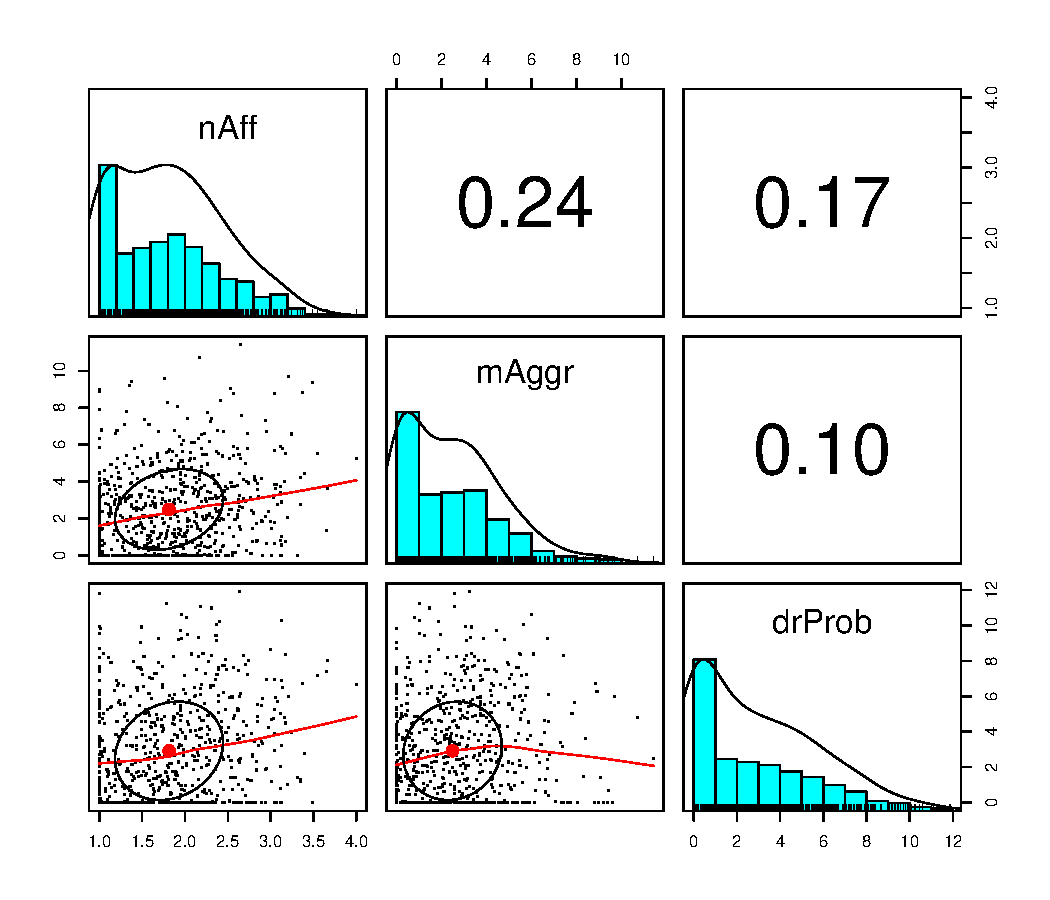
\includegraphics{03-Preliminaries_files/figure-latex/unnamed-chunk-59-1.pdf} What do we observe?

\begin{itemize}
\tightlist
\item
  There is a more-or-less moderate correlation between negative affect and microaggressions (\(r = 0.27\))
\item
  There is a small-to-moderate correlation between negative affect and drinking problems (\(r = 0.18\))
\item
  There is a small correlation between microaggressions and drinking problems (\(r = 0.09\))
\item
  All variables have a positive skew (with pile-up of scores on the lower end and tail pulling to the right); this is consistent with the values we calculated earlier
\item
  The scatterplots can provide clues to relations that are not necessarily linear.

  \begin{itemize}
  \tightlist
  \item
    Look at the relationship between negative affect and drinking problems. As negative affect hits around 2.75, there is a change in the relationship, such that drinking problems increase.
  \item
    Taking time to look at plots such as these can inform subsequent analyses.
  \end{itemize}
\end{itemize}

\hypertarget{apatables}{%
\subsection{apaTables}\label{apatables}}

Writing up an APA style results section frequently involves tables. A helpful package for doing this is \emph{apaTables}. An instructional article notes the contributions of tools like this to the \emph{reproducibility} of science by reducing errors made when the author or analyst retypes or copies text from output to the manuscript. When the R script is shared through an open science framework, reproducibility is further enhanced \citep{stanley_reproducible_2018}.

We pass the desired df to the \emph{apaTables::apa.cor.table}. Commands allow us to specify what is included in the table and whether it should be displayed in the console or saved as a document to the project's folder.

\begin{Shaded}
\begin{Highlighting}[]
\CommentTok{\# the apa.cor.table function removes any categorical variables that}
\CommentTok{\# might be in the df}
\NormalTok{Table1\_Cor }\OtherTok{\textless{}{-}}\NormalTok{ apaTables}\SpecialCharTok{::}\FunctionTok{apa.cor.table}\NormalTok{(df\_3vars, }\AttributeTok{filename =} \StringTok{"Table1\_Cor.doc"}\NormalTok{,}
    \AttributeTok{table.number =} \DecValTok{1}\NormalTok{, }\AttributeTok{show.conf.interval =} \ConstantTok{FALSE}\NormalTok{, }\AttributeTok{landscape =} \ConstantTok{TRUE}\NormalTok{)}
\end{Highlighting}
\end{Shaded}

\begin{verbatim}
The ability to suppress reporting of reporting confidence intervals has been deprecated in this version.
The function argument show.conf.interval will be removed in a later version.
\end{verbatim}

\begin{Shaded}
\begin{Highlighting}[]
\CommentTok{\# swap in this command to see it in the R Markdown file}
\FunctionTok{print}\NormalTok{(Table1\_Cor)}
\end{Highlighting}
\end{Shaded}

\begin{verbatim}


Table 1 

Means, standard deviations, and correlations with confidence intervals
 

  Variable  M    SD   1          2         
  1. nAff   1.81 0.63                      
                                           
  2. mAggr  2.49 2.19 .24**                
                      [.17, .31]           
                                           
  3. drProb 2.92 2.78 .17**      .10*      
                      [.10, .24] [.02, .17]
                                           

Note. M and SD are used to represent mean and standard deviation, respectively.
Values in square brackets indicate the 95% confidence interval.
The confidence interval is a plausible range of population correlations 
that could have caused the sample correlation (Cumming, 2014).
 * indicates p < .05. ** indicates p < .01.
 
\end{verbatim}

Because I added: \emph{filename = ``Table1\_Cor.doc''}, a word version of the table will appear in the same file folder as the .rmd file and data. It is easily manipulated with tools in your word processing package.

\hypertarget{an-apa-style-writeup}{%
\section{An APA Style Writeup}\label{an-apa-style-writeup}}

The statistics used in this lesson are often presented in the preliminary results portion of an empirical manuscript. Some of the results are written in text and some are presented in tables. APA Style recommends that the narration of results not duplicate what is presented in the tables. Rather, the write-up only highlights and clarifies what is presented in the table(s).

At the outset, let me note that a primary purpose of the Lui \citeyearpar{lui_racial_2020} article was to compare the relations of variables between three racial/ethic groups in the U.S. identified as Asian American, Black, and Latinx. Because we did not run separate analyses for each of the groups, my write-up does not make these distinctions. I highly recommend that you examine the write-up of results and the accompanying tables in Lui's article. The presentation is clear and efficient (i.e., it conveys maximal information in as little space as possible).

Below is an example of how I might write up these preliminary results:

\textbf{Preliminary Results}

\begin{quote}
Our sample included 713 participants who self-identified as Asian American, Black/African American, and Latinx American. Inspection of the characteristics of the three variables of interest (negative affect, microaggressions, drinking problems) indicated that all variables were positively skewed, however the values of skew and kurtosis did not exceed commonly used thressholds of concern \citep{kline_data_2016}. In contrast, Shapiro-Wilk tests of normality suggested that the distribution of all three variables were statistically significantly different than a normal distribution (\(nAff: W = 0.948, p < .001\); \(mAggr: W = 0.913, p < .001\); \(drProb: W = 0.900, p < .001\)). Means, standard deviations, and a correlation matrix are presented in Table 1. We noted that the correlation between negative affect and microaggressions was moderate \((r = 0.27)\); correlations between remaining variables were smaller.
\end{quote}

\hypertarget{practice-problems-1}{%
\section{Practice Problems}\label{practice-problems-1}}

The three exercises described below are designed to ``meet you where you are'' and allow you to challenge your skills depending on your goals as well as your comfort with statistics and R.

Regardless which you choose, work one or more of the problems with R packages:

\begin{itemize}
\tightlist
\item
  Create a smaller df from a larger df selecting a minimum of three continuously scaled variables
\item
  Calculate and interpret descriptive statistics
\item
  Create the SPLOM (pairs.panels)
\item
  Use the \emph{apaTables} package to make an APA style table with means, standard deviations, and correlations
\item
  Write an APA Style results section for these preliminary analyses
\end{itemize}

Additionally, please complete at least one set of \emph{hand calculations}, that is using the code demonstrated in the chapter to work through the formulas that compute the descriptive statistics that are the focus of this lesson. At this stage in your learning, you may ignore any missingness in your dataset by excluding all rows with missing data in your variables of interest.

\hypertarget{problem-1-change-the-random-seed}{%
\subsection{Problem \#1: Change the Random Seed}\label{problem-1-change-the-random-seed}}

If this topic feels a bit overwhelming, simply change the random seed in the data simulation (at the very top), then rework the lesson exactly as written. This should provide minor changes to the data (maybe in the second or third decimal point), but the results will likely be very similar.

\hypertarget{problem-2-swap-variables-in-the-simulation}{%
\subsection{Problem \#2: Swap Variables in the Simulation}\label{problem-2-swap-variables-in-the-simulation}}

Use the simulated data from the Lui \citeyearpar{lui_racial_2020} study. However, select three continuous variables (2 must be different from mine) and then conduct the analyses. Be sure to select from the variables that are considered to be \emph{continuous} (and not \emph{categorical}).

\hypertarget{problem-3-use-or-simulate-your-own-data}{%
\subsection{Problem \#3: Use (or Simulate) Your Own Data}\label{problem-3-use-or-simulate-your-own-data}}

Use data for which you have permission and access. This could be IRB approved data you have collected or from your lab; data you simulate from a published article; data from an open science repository; or data from other chapters in this OER.

\hypertarget{grading-rubrics}{%
\subsection{Grading Rubrics}\label{grading-rubrics}}

Regardless which option(s) you chose, use the elements in the grading rubrics to guide you through the practice. Worked examples are provided in the \href{\%7B\#woRked\%7D}{Appendix}.

\begin{longtable}[]{@{}
  >{\raggedright\arraybackslash}p{(\columnwidth - 4\tabcolsep) * \real{0.5833}}
  >{\centering\arraybackslash}p{(\columnwidth - 4\tabcolsep) * \real{0.2083}}
  >{\raggedright\arraybackslash}p{(\columnwidth - 4\tabcolsep) * \real{0.2083}}@{}}
\toprule\noalign{}
\begin{minipage}[b]{\linewidth}\raggedright
Working the problem with R and R packages
\end{minipage} & \begin{minipage}[b]{\linewidth}\centering
Points Poss
\end{minipage} & \begin{minipage}[b]{\linewidth}\raggedright
Points Earned
\end{minipage} \\
\midrule\noalign{}
\endhead
\bottomrule\noalign{}
\endlastfoot
1. Create a df with 3 continuously scaled variables of interest & 3 & \\
2. Produce descriptive statistics & 3 & \\
3. Produce SPLOM/pairs.panels & 3 & \\
4. Produce an apaTables matrix & 3 & \\
5. Produce an APA Style write-up of the preliminary analyses & 5 & \\
6. Explanation/discussion with a grader & 5 & \\
**Totals & 22 & \\
\end{longtable}

\begin{longtable}[]{@{}
  >{\raggedright\arraybackslash}p{(\columnwidth - 4\tabcolsep) * \real{0.5833}}
  >{\centering\arraybackslash}p{(\columnwidth - 4\tabcolsep) * \real{0.2083}}
  >{\raggedright\arraybackslash}p{(\columnwidth - 4\tabcolsep) * \real{0.2083}}@{}}
\toprule\noalign{}
\begin{minipage}[b]{\linewidth}\raggedright
Hand Calculations
\end{minipage} & \begin{minipage}[b]{\linewidth}\centering
Points Poss
\end{minipage} & \begin{minipage}[b]{\linewidth}\raggedright
Points Earned
\end{minipage} \\
\midrule\noalign{}
\endhead
\bottomrule\noalign{}
\endlastfoot
1. Create a variable that represents the mean. & 2 & \\
2. Create a variable that represents the mean deviation. & 2 & \\
3. What is the value of the \emph{sum} of mean deviations? & 2 & \\
4. Create a variable that represents the absolute mean deviation. What is the \emph{sum} of the absolute mean deviation? What is the value of the \emph{mean} of the absolute mean deviation? What does this value tell you? & 4 & \\
5. Create a variable that represents the mean deviation squared. & 2 & \\
6. What are the values of the sum of squared deviations around the mean \(SS\), variance \(s^2\), and standard deviation (\(s\))? & 3 & \\
7. Using the same general approach, calculate the mean deviation and standard deviation for a second, continuously scaled variable. & 5 & \\
8. Create a variable that represents the \emph{cross-product} (of the mean deviations). What is the sum of these cross-products? & 2 & \\
9. Calculate the value of their covariance. & 2 & \\
8. Calculate value of correlation coefficient. & 2 & \\
**Totals & 26 & \\
\end{longtable}

\hypertarget{homeworked-example-1}{%
\section{Homeworked Example}\label{homeworked-example-1}}

\href{}{Screencast Link}

Preliminary analyses often consist of means, standard deviations, and correlations. These can be helpful in determining whether or not data are normally distribution. Correlations and pairs.panels also assess the relatedness of the variables.

\emph{If you wanted to use this example and dataset as a basis for a homework assignment, you could (a) select a different course (i.e., Multivariate or Psychometrics) and/or (b) different variables.}

\hypertarget{working-the-problem-with-r-and-r-packages}{%
\subsection{Working the Problem with R and R Packages}\label{working-the-problem-with-r-and-r-packages}}

\hypertarget{create-a-df-with-3-continuously-scaled-variables-of-interest}{%
\subsubsection{Create a df with 3 continuously scaled variables of interest}\label{create-a-df-with-3-continuously-scaled-variables-of-interest}}

The ReC.rds is the entire dataset. Let's first open it.

\begin{Shaded}
\begin{Highlighting}[]
\NormalTok{ReCdf }\OtherTok{\textless{}{-}} \FunctionTok{readRDS}\NormalTok{(}\StringTok{"ReC.rds"}\NormalTok{)}
\end{Highlighting}
\end{Shaded}

Recall that students (represented by the \emph{deID} variable) could contribute up to three course evaluations (i.e., ANOVA, psychometrics, multivariate) each. In many statistics, repeated observations creates dependencies that need to be accounted for statistically.

To avoid this dependency and to practice an R skil, let's first filter the data, selecting only those students who took ANOVA.

\begin{Shaded}
\begin{Highlighting}[]
\NormalTok{JustANOVA }\OtherTok{\textless{}{-}} \FunctionTok{subset}\NormalTok{(ReCdf, Course }\SpecialCharTok{==} \StringTok{"ANOVA"}\NormalTok{) }
\end{Highlighting}
\end{Shaded}

\hypertarget{create-a-df-with-3-continuously-scaled-variables-of-interest-1}{%
\subsubsection{Create a df with 3 continuously scaled variables of interest}\label{create-a-df-with-3-continuously-scaled-variables-of-interest-1}}

The assignment requires that we downsize to three variables. We could pick any three.

\begin{Shaded}
\begin{Highlighting}[]
\FunctionTok{library}\NormalTok{(tidyverse)}
\NormalTok{tiny3 }\OtherTok{\textless{}{-}}\NormalTok{ JustANOVA }\SpecialCharTok{\%\textgreater{}\%}
\NormalTok{    dplyr}\SpecialCharTok{::}\FunctionTok{select}\NormalTok{ (OvInstructor, OvCourse, MyContribution)}
\end{Highlighting}
\end{Shaded}

\hypertarget{produce-descriptive-statistics}{%
\subsubsection{Produce descriptive statistics}\label{produce-descriptive-statistics}}

\begin{Shaded}
\begin{Highlighting}[]
\NormalTok{psych}\SpecialCharTok{::}\FunctionTok{describe}\NormalTok{(tiny3)}
\end{Highlighting}
\end{Shaded}

\begin{verbatim}
               vars   n mean   sd median trimmed  mad min max range  skew
OvInstructor      1 113 4.19 1.01      5    4.34 0.00   1   5     4 -0.98
OvCourse          2 113 3.93 1.12      4    4.07 1.48   1   5     4 -0.72
MyContribution    3 113 3.96 0.83      4    4.01 1.48   2   5     3 -0.39
               kurtosis   se
OvInstructor      -0.07 0.10
OvCourse          -0.49 0.11
MyContribution    -0.55 0.08
\end{verbatim}

\hypertarget{produce-splompairs.panels}{%
\subsubsection{Produce SPLOM/pairs.panels}\label{produce-splompairs.panels}}

\begin{Shaded}
\begin{Highlighting}[]
\NormalTok{psych}\SpecialCharTok{::}\FunctionTok{pairs.panels}\NormalTok{(tiny3)}
\end{Highlighting}
\end{Shaded}

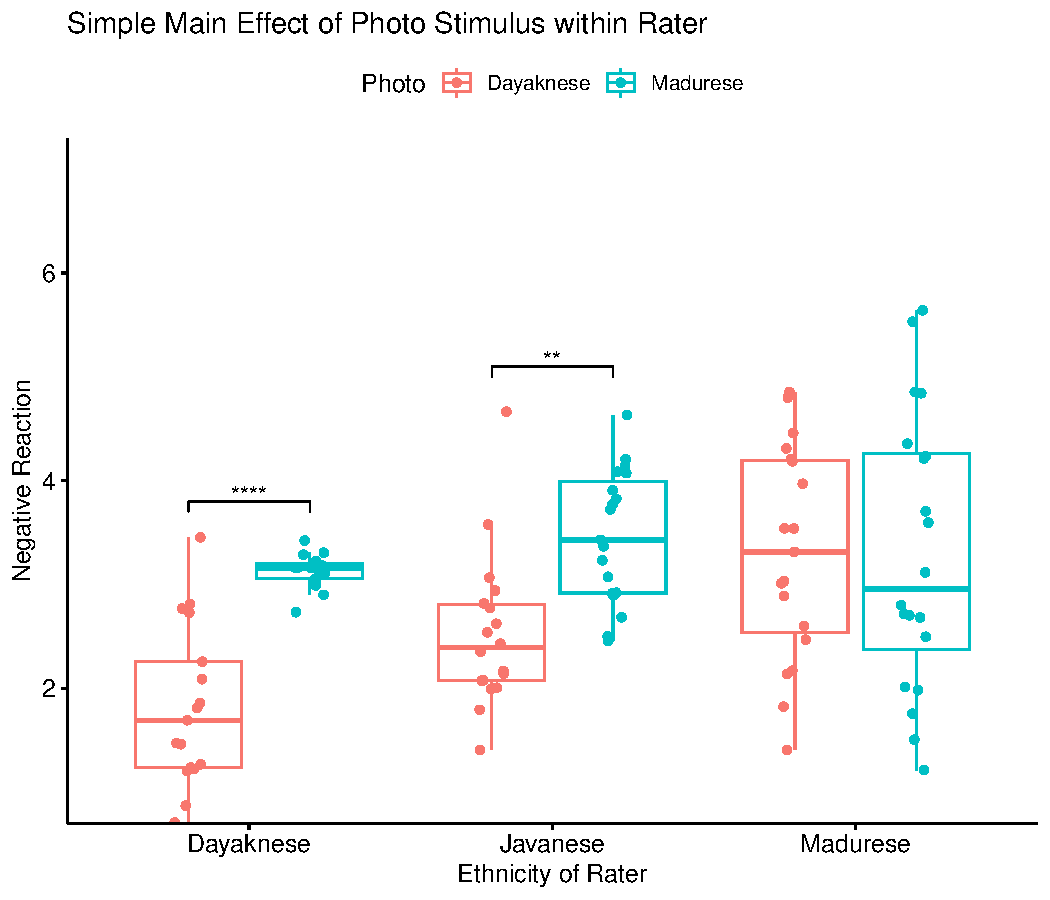
\includegraphics{03-Preliminaries_files/figure-latex/unnamed-chunk-67-1.pdf}

\hypertarget{produce-an-apatables-matrix}{%
\subsubsection{Produce an apaTables matrix}\label{produce-an-apatables-matrix}}

\begin{Shaded}
\begin{Highlighting}[]
\NormalTok{apaTables}\SpecialCharTok{::}\FunctionTok{apa.cor.table}\NormalTok{(tiny3)}
\end{Highlighting}
\end{Shaded}

\begin{verbatim}


Means, standard deviations, and correlations with confidence intervals
 

  Variable          M    SD   1          2         
  1. OvInstructor   4.19 1.01                      
                                                   
  2. OvCourse       3.93 1.12 .83**                
                              [.76, .88]           
                                                   
  3. MyContribution 3.96 0.83 .49**      .60**     
                              [.34, .62] [.46, .70]
                                                   

Note. M and SD are used to represent mean and standard deviation, respectively.
Values in square brackets indicate the 95% confidence interval.
The confidence interval is a plausible range of population correlations 
that could have caused the sample correlation (Cumming, 2014).
 * indicates p < .05. ** indicates p < .01.
 
\end{verbatim}

\hypertarget{produce-an-apa-style-write-up-of-the-preliminary-analyses}{%
\subsubsection{Produce an APA Style write-up of the preliminary analyses}\label{produce-an-apa-style-write-up-of-the-preliminary-analyses}}

Our sample included 113 doctoral students in Clinical and Industrial-Organizational psychology doctoral (PhD) programs who were completing a statistics class focused on analysis of variance. Visual inspection of three dimensions of course evaluation (overall instructor, overall course, my contributions) combined with formal evaluation of skewness and kurtosis suggested that their distributions did not violate the assumption of univariate normality. That is, skew values all fell below the absolute value of 3 and kurtosis values all fell below the absolute value of 10 \citep{kline_data_2016}. Means, standard deviations, and a correlation matrix are presented in Table 1. All three correlations were strong and statistically significant. We noted that the correlation between the overall instructor and overall course was especially high (\emph{r} = .83, \emph{p} \textless{} .001)

\hypertarget{hand-calculations}{%
\subsection{Hand Calculations}\label{hand-calculations}}

Although these are termed ``hand calculations,'' you may use the code demonstrated in the chapter to work these problems.

I am going to continue with the \emph{tiny3} dataset I used when I worked the problem with R and R packages. Given that this is for homework, let's avoid problems with missingness by deleting any rows with missing data:

If you need to reimport data, here is a quick recap of the code explained earlier.

\begin{Shaded}
\begin{Highlighting}[]
\NormalTok{ReCdf }\OtherTok{\textless{}{-}} \FunctionTok{readRDS}\NormalTok{(}\StringTok{"ReC.rds"}\NormalTok{)}
\NormalTok{JustANOVA }\OtherTok{\textless{}{-}} \FunctionTok{subset}\NormalTok{(ReCdf, Course }\SpecialCharTok{==} \StringTok{"ANOVA"}\NormalTok{) }

\FunctionTok{library}\NormalTok{(tidyverse)}
\NormalTok{tiny3 }\OtherTok{\textless{}{-}}\NormalTok{ JustANOVA }\SpecialCharTok{\%\textgreater{}\%}
\NormalTok{    dplyr}\SpecialCharTok{::}\FunctionTok{select}\NormalTok{ (OvInstructor, OvCourse, MyContribution)}
\end{Highlighting}
\end{Shaded}

To avoid problems in the code we are used that is caused by missingness, we will eliminate any rows with missing data.

\begin{Shaded}
\begin{Highlighting}[]
\NormalTok{tiny3 }\OtherTok{\textless{}{-}} \FunctionTok{na.omit}\NormalTok{(tiny3)}
\end{Highlighting}
\end{Shaded}

\hypertarget{create-a-variable-that-represents-the-mean.}{%
\subsubsection{Create a variable that represents the mean.}\label{create-a-variable-that-represents-the-mean.}}

I will start with the OvInstructor variable. Inspect the dataframe to see that this new variable exists.

\begin{Shaded}
\begin{Highlighting}[]
\NormalTok{tiny3}\SpecialCharTok{$}\NormalTok{M\_OvI }\OtherTok{\textless{}{-}} \FunctionTok{mean}\NormalTok{(tiny3}\SpecialCharTok{$}\NormalTok{OvInstructor, }\AttributeTok{na.rm=}\ConstantTok{TRUE}\NormalTok{)}
\end{Highlighting}
\end{Shaded}

\hypertarget{create-a-variable-that-represents-the-mean-deviation.}{%
\subsubsection{Create a variable that represents the mean deviation.}\label{create-a-variable-that-represents-the-mean-deviation.}}

\begin{Shaded}
\begin{Highlighting}[]
\NormalTok{tiny3}\SpecialCharTok{$}\NormalTok{Mdev\_OvI }\OtherTok{\textless{}{-}}\NormalTok{ (tiny3}\SpecialCharTok{$}\NormalTok{OvInstructor}\SpecialCharTok{{-}}\NormalTok{tiny3}\SpecialCharTok{$}\NormalTok{M\_OvI)}
\end{Highlighting}
\end{Shaded}

Inspect the dataframe to see that this new variable exists. Note that this functions to ``center'' the mean around zero.

\hypertarget{what-is-the-value-of-the-sum-of-mean-deviations}{%
\subsubsection{What is the value of the sum of mean deviations?}\label{what-is-the-value-of-the-sum-of-mean-deviations}}

\begin{Shaded}
\begin{Highlighting}[]
\FunctionTok{round}\NormalTok{(}\FunctionTok{sum}\NormalTok{(tiny3}\SpecialCharTok{$}\NormalTok{Mdev\_OvI, }\AttributeTok{na.rm =} \ConstantTok{TRUE}\NormalTok{), }\DecValTok{3}\NormalTok{)}
\end{Highlighting}
\end{Shaded}

\begin{verbatim}
[1] 0
\end{verbatim}

Yes, zero!

\hypertarget{create-a-variable-that-represents-the-absolute-mean-deviation.}{%
\subsubsection{Create a variable that represents the absolute mean deviation.}\label{create-a-variable-that-represents-the-absolute-mean-deviation.}}

\begin{Shaded}
\begin{Highlighting}[]
\NormalTok{tiny3}\SpecialCharTok{$}\NormalTok{abslt\_mOvI }\OtherTok{\textless{}{-}} \FunctionTok{abs}\NormalTok{(tiny3}\SpecialCharTok{$}\NormalTok{Mdev\_OvI)}
\end{Highlighting}
\end{Shaded}

Inspect the dataframe to see that this new variable no longer has negative values.

\textbf{What is the value of the sum of the absolute mean deviation?}

\begin{Shaded}
\begin{Highlighting}[]
\FunctionTok{round}\NormalTok{(}\FunctionTok{sum}\NormalTok{(tiny3}\SpecialCharTok{$}\NormalTok{abslt\_mOvI, }\AttributeTok{na.rm =} \ConstantTok{TRUE}\NormalTok{), }\DecValTok{3}\NormalTok{)}
\end{Highlighting}
\end{Shaded}

\begin{verbatim}
[1] 96.071
\end{verbatim}

\textbf{What is the value of the mean of the absolute mean deviation?}

\begin{Shaded}
\begin{Highlighting}[]
\FunctionTok{round}\NormalTok{(}\FunctionTok{mean}\NormalTok{(tiny3}\SpecialCharTok{$}\NormalTok{abslt\_mOvI, }\AttributeTok{na.rm =} \ConstantTok{TRUE}\NormalTok{), }\DecValTok{3}\NormalTok{)}
\end{Highlighting}
\end{Shaded}

\begin{verbatim}
[1] 0.85
\end{verbatim}

\textbf{What does this value tell you?}

Average distance of each value from the mean.

\hypertarget{create-a-variable-that-represents-the-mean-deviation-squared.}{%
\subsubsection{Create a variable that represents the mean deviation squared.}\label{create-a-variable-that-represents-the-mean-deviation-squared.}}

\begin{Shaded}
\begin{Highlighting}[]
\NormalTok{tiny3}\SpecialCharTok{$}\NormalTok{mdev2\_OvI }\OtherTok{\textless{}{-}}\NormalTok{ (tiny3}\SpecialCharTok{$}\NormalTok{Mdev\_OvI }\SpecialCharTok{*}\NormalTok{ tiny3}\SpecialCharTok{$}\NormalTok{Mdev\_OvI)}
\end{Highlighting}
\end{Shaded}

\textbf{What is the value of the sum of squared deviations around the mean (also known as sums of squares; sometimes abbreviated as \(SS\))?}

\begin{Shaded}
\begin{Highlighting}[]
\FunctionTok{sum}\NormalTok{(tiny3}\SpecialCharTok{$}\NormalTok{mdev2\_OvI, }\AttributeTok{na.rm =} \ConstantTok{TRUE}\NormalTok{)}
\end{Highlighting}
\end{Shaded}

\begin{verbatim}
[1] 115.0973
\end{verbatim}

\textbf{What is the value of the variance (\(s^2\))?}

There are at least two ways to do this with basic code (and then we can check our work).

Here's how to do it with ``more code.''

\begin{Shaded}
\begin{Highlighting}[]
\NormalTok{var\_OvI }\OtherTok{\textless{}{-}} \FunctionTok{sum}\NormalTok{(tiny3}\SpecialCharTok{$}\NormalTok{mdev2\_OvI}\SpecialCharTok{/}\NormalTok{((}\FunctionTok{nrow}\NormalTok{(tiny3) }\SpecialCharTok{{-}} \DecValTok{1}\NormalTok{)))}
\NormalTok{var\_OvI}
\end{Highlighting}
\end{Shaded}

\begin{verbatim}
[1] 1.027655
\end{verbatim}

Here's how to do it with the numbers that I calculated:

\begin{Shaded}
\begin{Highlighting}[]
\FloatTok{115.0973}\SpecialCharTok{/}\NormalTok{(}\DecValTok{113{-}1}\NormalTok{)}
\end{Highlighting}
\end{Shaded}

\begin{verbatim}
[1] 1.027654
\end{verbatim}

Checking my work with the \emph{var} function from base R. If it's wrong, I need to rework some of the previous steps.

\begin{Shaded}
\begin{Highlighting}[]
\FunctionTok{var}\NormalTok{(tiny3}\SpecialCharTok{$}\NormalTok{OvInstructor, }\AttributeTok{na.rm =} \ConstantTok{TRUE}\NormalTok{) }\CommentTok{\#checking my work}
\end{Highlighting}
\end{Shaded}

\begin{verbatim}
[1] 1.027655
\end{verbatim}

\textbf{What is the value of the standard deviation (\(s\))?}

There are two ways to calculate it with basic code; and then we can check it with more code from base R.

\begin{Shaded}
\begin{Highlighting}[]
\NormalTok{sd\_OvI }\OtherTok{\textless{}{-}} \FunctionTok{sqrt}\NormalTok{(var\_OvI)}\CommentTok{\#calculating with the object I created}
\NormalTok{sd\_OvI}
\end{Highlighting}
\end{Shaded}

\begin{verbatim}
[1] 1.013733
\end{verbatim}

\begin{Shaded}
\begin{Highlighting}[]
\FunctionTok{sqrt}\NormalTok{ (}\FloatTok{1.027655}\NormalTok{)}\CommentTok{\#calculated with the actual numbers}
\end{Highlighting}
\end{Shaded}

\begin{verbatim}
[1] 1.013733
\end{verbatim}

\begin{Shaded}
\begin{Highlighting}[]
\FunctionTok{sd}\NormalTok{(tiny3}\SpecialCharTok{$}\NormalTok{OvInstructor)}\CommentTok{\#checking my work with the code from baseR}
\end{Highlighting}
\end{Shaded}

\begin{verbatim}
[1] 1.013733
\end{verbatim}

\hypertarget{using-the-same-general-approach-calculate-the-mean-deviation-and-standard-deviation-for-a-second-continuously-scaled-variable.}{%
\subsubsection{Using the same general approach, calculate the mean deviation and standard deviation for a second, continuously scaled variable.}\label{using-the-same-general-approach-calculate-the-mean-deviation-and-standard-deviation-for-a-second-continuously-scaled-variable.}}

My second variable is MyContribution

\begin{Shaded}
\begin{Highlighting}[]
\CommentTok{\#first the mean}
\NormalTok{tiny3}\SpecialCharTok{$}\NormalTok{M\_MyC }\OtherTok{\textless{}{-}} \FunctionTok{mean}\NormalTok{(tiny3}\SpecialCharTok{$}\NormalTok{MyContribution, }\AttributeTok{na.rm=}\ConstantTok{TRUE}\NormalTok{)}
\CommentTok{\#second the mean deviation}
\NormalTok{tiny3}\SpecialCharTok{$}\NormalTok{Mdev\_MyC }\OtherTok{\textless{}{-}}\NormalTok{ (tiny3}\SpecialCharTok{$}\NormalTok{MyContribution}\SpecialCharTok{{-}}\NormalTok{tiny3}\SpecialCharTok{$}\NormalTok{M\_MyC)}

\CommentTok{\#fourth the variance}
\NormalTok{var\_MyC }\OtherTok{\textless{}{-}} \FunctionTok{sum}\NormalTok{(tiny3}\SpecialCharTok{$}\NormalTok{mdev2\_MyC}\SpecialCharTok{/}\NormalTok{((}\FunctionTok{nrow}\NormalTok{(tiny3) }\SpecialCharTok{{-}} \DecValTok{1}\NormalTok{)))}
\NormalTok{var\_MyC}
\end{Highlighting}
\end{Shaded}

\begin{verbatim}
[1] 0
\end{verbatim}

\begin{Shaded}
\begin{Highlighting}[]
\CommentTok{\#finally the standard deviation}
\NormalTok{sd\_MyC }\OtherTok{\textless{}{-}} \FunctionTok{sqrt}\NormalTok{(var\_MyC)}
\NormalTok{sd\_MyC}\CommentTok{\#checking my work}
\end{Highlighting}
\end{Shaded}

\begin{verbatim}
[1] 0
\end{verbatim}

\begin{Shaded}
\begin{Highlighting}[]
\FunctionTok{sd}\NormalTok{(tiny3}\SpecialCharTok{$}\NormalTok{MyContribution)}\CommentTok{\#checking my work}
\end{Highlighting}
\end{Shaded}

\begin{verbatim}
[1] 0.8337652
\end{verbatim}

\hypertarget{create-a-variable-that-represents-the-cross-product-of-the-mean-deviations.-what-is-the-sum-of-these-cross-products}{%
\subsubsection{\texorpdfstring{Create a variable that represents the \emph{cross-product} (of the mean deviations). What is the sum of these cross-products?}{Create a variable that represents the cross-product (of the mean deviations). What is the sum of these cross-products?}}\label{create-a-variable-that-represents-the-cross-product-of-the-mean-deviations.-what-is-the-sum-of-these-cross-products}}

\begin{Shaded}
\begin{Highlighting}[]
\NormalTok{tiny3}\SpecialCharTok{$}\NormalTok{crossproduct }\OtherTok{\textless{}{-}}\NormalTok{ (tiny3}\SpecialCharTok{$}\NormalTok{Mdev\_OvI }\SpecialCharTok{*}\NormalTok{ tiny3}\SpecialCharTok{$}\NormalTok{Mdev\_MyC)}
\end{Highlighting}
\end{Shaded}

The sum of the crossproduct is:

\begin{Shaded}
\begin{Highlighting}[]
\NormalTok{xp\_sum }\OtherTok{\textless{}{-}} \FunctionTok{sum}\NormalTok{(tiny3}\SpecialCharTok{$}\NormalTok{crossproduct)}
\NormalTok{xp\_sum}
\end{Highlighting}
\end{Shaded}

\begin{verbatim}
[1] 46.74336
\end{verbatim}

\hypertarget{calculate-the-value-of-their-covariance.}{%
\subsubsection{Calculate the value of their covariance.}\label{calculate-the-value-of-their-covariance.}}

\begin{Shaded}
\begin{Highlighting}[]
\NormalTok{cov }\OtherTok{\textless{}{-}}\NormalTok{ (}\DecValTok{1}\SpecialCharTok{/}\NormalTok{(}\DecValTok{113{-}1}\NormalTok{)) }\SpecialCharTok{*} \FloatTok{46.74336}
\NormalTok{cov}
\end{Highlighting}
\end{Shaded}

\begin{verbatim}
[1] 0.4173514
\end{verbatim}

\hypertarget{calculate-value-of-correlation-coefficient.}{%
\subsubsection{Calculate value of correlation coefficient.}\label{calculate-value-of-correlation-coefficient.}}

\begin{Shaded}
\begin{Highlighting}[]
\FloatTok{0.4173514}\SpecialCharTok{/}\NormalTok{(}\FloatTok{1.013733}\SpecialCharTok{*}\FloatTok{0.8338}\NormalTok{)}
\end{Highlighting}
\end{Shaded}

\begin{verbatim}
[1] 0.4937606
\end{verbatim}

And now I can check my work with a function from base R.

\begin{Shaded}
\begin{Highlighting}[]
\FunctionTok{cor.test}\NormalTok{(tiny3}\SpecialCharTok{$}\NormalTok{OvInstructor, tiny3}\SpecialCharTok{$}\NormalTok{MyContribution)}
\end{Highlighting}
\end{Shaded}

\begin{verbatim}

    Pearson's product-moment correlation

data:  tiny3$OvInstructor and tiny3$MyContribution
t = 5.9825, df = 111, p-value = 0.00000002737
alternative hypothesis: true correlation is not equal to 0
95 percent confidence interval:
 0.3400714 0.6217934
sample estimates:
      cor 
0.4937812 
\end{verbatim}

The correlation between ratings of overall instructor and my contribution is 0.493, \(p < .001\).

\hypertarget{t-tests}{%
\chapter*{\texorpdfstring{\emph{t}-tests}{t-tests}}\label{t-tests}}


The lessons offered in the \emph{t}-tests section introduce \emph{inferential statistics}. In the prior chapters, our use of measures of central tendency (i.e., mean, median, mode) and variance (i.e., range, variance, standard deviation) serve to \emph{describe} a sample.

As we move into \emph{inferential} statistics we evaluate data from a sample and try to determine whether or not we can use it to draw conclusions (i.e, predict or make inferences) about a larger, defined, population.

The \emph{t}-test lessons begin with an explanation of the \emph{z}-score and progress through one sample, independent samples, and paired samples \emph{t}-tests. Each lesson is centered around a research vignette that was focused on physicians' communication with patients who were critically and terminally ill and in the intensive care unit at a hospial \citep{elliott_differences_2016}.

In addition to a conceptual presentation of of each statistic, each lesson includes:

\begin{itemize}
\tightlist
\item
  a workflow that guides researchers through decision-points in each statistic,
\item
  the presentation of formulas and R code for ``hand-calculating'' each component of the formula,
\item
  script for efficiently computing the statistic with R packages,
\item
  an ``recipe'' for an APA style presentation of the results,
\item
  a discussion of \emph{power} in that particular statistic with R script for calculating sample sizes sufficient to reject the null hypothesis, if in fact, it is appropriate to do so, and
\item
  suggestions for practice that vary in degree of challenge.
\end{itemize}

\hypertarget{tOneSample}{%
\chapter{\texorpdfstring{One Sample \emph{t}-tests}{One Sample t-tests}}\label{tOneSample}}

\href{https://spu.hosted.panopto.com/Panopto/Pages/Viewer.aspx?pid=c029edfb-4215-44be-972d-af0100365877}{Screencasted Lecture Link}

\begin{Shaded}
\begin{Highlighting}[]
\FunctionTok{options}\NormalTok{(}\AttributeTok{scipen =} \DecValTok{999}\NormalTok{)  }\CommentTok{\#eliminates scientific notation}
\end{Highlighting}
\end{Shaded}

Researchers and program evaluators, may wish to know if their data differs from an external standard. In today's research vignette, we will ask if the time physicians spent with their patients differed from an external benchmark. The one sample \emph{t}-test is an appropriate tool for this type of analysis. As we work toward the one sample \emph{t}-test we take some time to explore the standard normal curve and \emph{z}-scores, particularly as they related to probability.

\hypertarget{navigating-this-lesson-2}{%
\section{Navigating this Lesson}\label{navigating-this-lesson-2}}

There is just over one hour of lecture. If you work through the materials with me, plan for an additional hour-and-a-half.

While the majority of R objects and data you will need are created within the R script that sources the chapter, occasionally there are some that cannot be created from within the R framework. Additionally, sometimes links fail. All original materials are provided at the \href{https://github.com/lhbikos/ReCenterPsychStats}{Github site} that hosts the book. More detailed guidelines for ways to access all these materials are provided in the OER's \protect\hyperlink{ReCintro}{introduction}

\hypertarget{learning-objectives-2}{%
\subsection{Learning Objectives}\label{learning-objectives-2}}

Learning objectives from this lecture include the following:

\begin{itemize}
\tightlist
\item
  Convert raw scores to \emph{z}-scores (and back again).
\item
  Using the \emph{z} table, determine the probability of an occurence.
\item
  Recognize the research questions for which utilization of a one sample \emph{t}-test would be appropriate.
\item
  Narrate the steps in conducting a one-sample \emph{t}-test, beginning with testing the statistical assumptions through writing up an APA style results section.
\item
  Calculate a one-sample \emph{t}-test in R (including effect sizes).
\item
  Interpret a 95\% confidence interval around a mean difference score.
\item
  Produce an APA style results section for a one-sample \emph{t}-test .
\item
  Determine a sample size that (given a set of parameters) would likely result in a statistically significant effect, if there was one.
\end{itemize}

\hypertarget{planning-for-practice-1}{%
\subsection{Planning for Practice}\label{planning-for-practice-1}}

The suggestions for homework vary in degree of complexity. The more complete descriptions at the end of the chapter follow these suggestions.

\begin{itemize}
\tightlist
\item
  Rework the one-sample \emph{t}-test in the lesson by changing the random seed in the code that simulates the data. This should provide minor changes to the data, but the results will likely be very similar.
\item
  Rework the one-sample \emph{t}-test in the lesson by changing something else about the simulation. For example, if you are interested in power, consider changing the sample size.
\item
  Conduct a one sample \emph{t}-test with data to which you have access and permission to use. This could include data you simulate on your own or from a published article.
\end{itemize}

\hypertarget{readings-resources-1}{%
\subsection{Readings \& Resources}\label{readings-resources-1}}

In preparing this chapter, I drew heavily from the following resource(s). Other resources are cited (when possible, linked) in the text with complete citations in the reference list.

\begin{itemize}
\tightlist
\item
  How To Do a One-Sample T-test in R: Best Tutorial You Need. (n.d.). Datanovia. Retrieved May 24, 2023, from \url{https://www.datanovia.com/en/lessons/how-to-do-a-t-test-in-r-calculation-and-reporting/how-to-do-a-one-sample-t-test-in-r/}

  \begin{itemize}
  \tightlist
  \item
    The primary R code we use is from the rstatix/Datanovia tutorial. *Navarro, D. (2020). Chapter 13: Comparing two means. In \href{https://learningstatisticswithr.com/}{Learning Statistics with R - A tutorial for Psychology Students and other Beginners}. Retrieved from \url{https://stats.libretexts.org/Bookshelves/Applied_Statistics/Book\%3A_Learning_Statistics_with_R_-_A_tutorial_for_Psychology_Students_and_other_Beginners_(Navarro)}
  \item
    Navarro's OER includes a good mix of conceptual information about \emph{t}-tests as well as R code. My lesson integrates her approach as well as considering information from Field's \citeyearpar{field_discovering_2012} and Green and Salkind's \citeyearpar{green_using_2017} texts.
  \end{itemize}
\item
  Elliott, A. M., Alexander, S. C., Mescher, C. A., Mohan, D., \& Barnato, A. E. (2016). Differences in Physicians' Verbal and Nonverbal Communication With Black and White Patients at the End of Life. \emph{Journal of Pain and Symptom Management, 51}(1), 1--8. \url{https://doi.org/10.1016/j.jpainsymman.2015.07.008}

  \begin{itemize}
  \tightlist
  \item
    The source of our research vignette.
  \end{itemize}
\end{itemize}

\hypertarget{packages}{%
\subsection{Packages}\label{packages}}

The script below will (a) check to see if the following packages are installed on your computer and, if not (b) install them. Remove the hashtags for the code to work.

\begin{Shaded}
\begin{Highlighting}[]
\CommentTok{\# will install the package if not already installed}
\CommentTok{\# if(!require(psych))\{install.packages(\textquotesingle{}psych\textquotesingle{})\}}
\CommentTok{\# if(!require(tidyverse))\{install.packages(\textquotesingle{}tidyverse\textquotesingle{})\}}
\CommentTok{\# if(!require(dplyr))\{install.packages(\textquotesingle{}dplyr\textquotesingle{})\}}
\CommentTok{\# if(!require(ggpubr))\{install.packages(\textquotesingle{}ggpubr\textquotesingle{})\}}
\CommentTok{\# if(!require(knitr))\{install.packages(\textquotesingle{}knitr\textquotesingle{})\}}
\CommentTok{\# if(!require(apaTables))\{install.packages(\textquotesingle{}apaTables\textquotesingle{})\}}
\CommentTok{\# if(!require(pwr))\{install.packages(\textquotesingle{}pwr\textquotesingle{})\}}
\CommentTok{\# if(!require(pastecs))\{install.packages(\textquotesingle{}pastecs\textquotesingle{})\}}
\CommentTok{\# if(!require(rstatix))\{install.packages(\textquotesingle{}rstatix\textquotesingle{})\}}
\end{Highlighting}
\end{Shaded}

\hypertarget{z-before-t}{%
\section{\texorpdfstring{\emph{z} before \emph{t}}{z before t}}\label{z-before-t}}

\textbf{Probability density functions} are mathematical formula that specifies idealized versions of known distributions. The equations that define these distributions allow us to calculate the probability of obtaining a given score. This is a powerful tool.

As students progress through statistics, they become familiar with a variety of these distributions including the \emph{t}-distribution (commonly used in \emph{t}-tests), \emph{F}-distribution (commonly used in analysis of variance {[}ANOVA{]}), and Chi-square (\(X^2\)) distributions (used in a variety of statistics, including structural equation modeling). The \emph{z} distribution is the most well-known of these distributions.

The \emph{z} distribution is also known as the normal distribution, the bell curve, or the standard normal curve. Its mean is always 0.00 and its standard deviation is always 1.00. Regardless of the actual mean and standard deviation:

\begin{itemize}
\tightlist
\item
  68.3\% of the area falls within 1 standard deviation of the mean
\item
  95.4\% of the distribution falls within 2 standard deviations of the mean
\item
  99.7\% of the distribution falls within 3 standard deviations of the mean
\end{itemize}

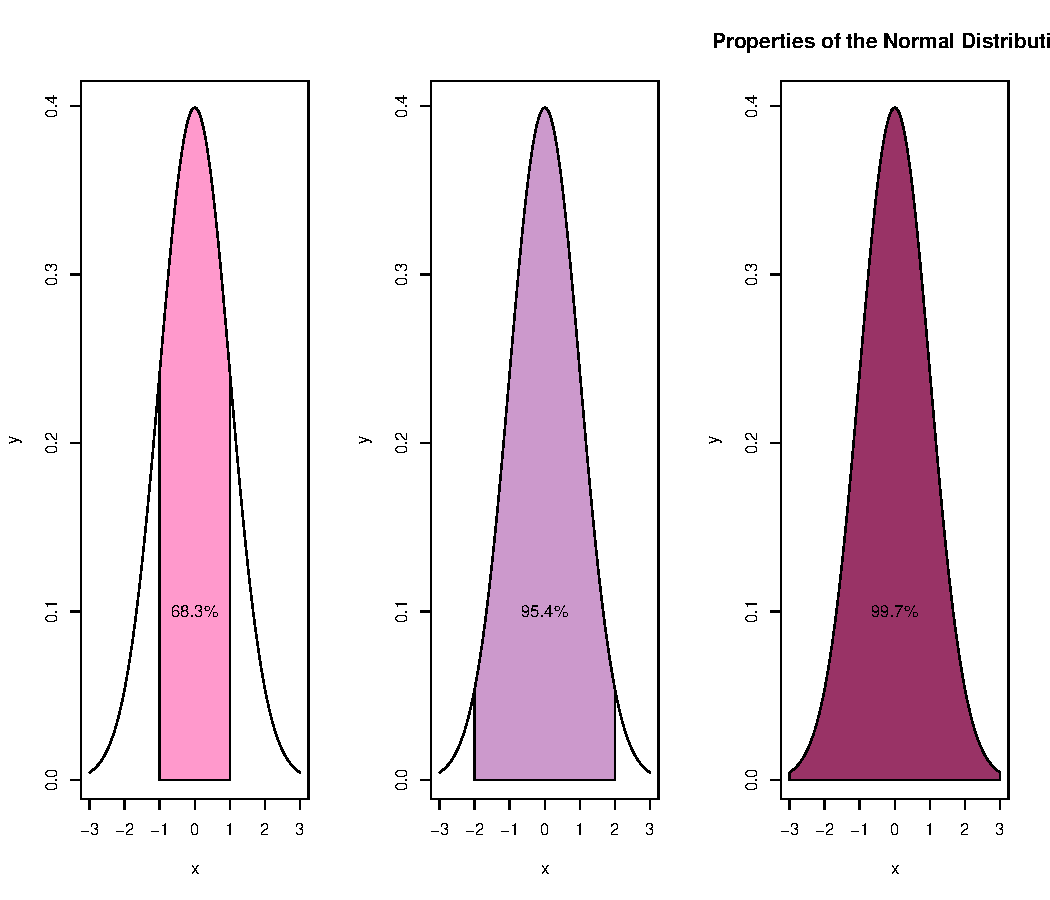
\includegraphics{04-tOneSample_files/figure-latex/unnamed-chunk-4-1.pdf} \emph{z}-scores are transformations of raw scores, in standard deviation units. Using the following formula, so long as the mean and standard deviation are known, any set of continuously scaled scores can be transformed to a \emph{z}-scores equivalent:

\[z=\frac{X-\bar{X}}{s}\] We can rearrange the formula to find what raw score corresponds with the \emph{z}-score.

\[X = \bar{X} + z(s)\]

The properties of the \emph{z}-score and the standard normal curve allow us to make inferences about the data.

\hypertarget{simulating-a-mini-research-vignette}{%
\subsection{Simulating a Mini Research Vignette}\label{simulating-a-mini-research-vignette}}

Later in this larger section on \emph{t}-tests we introduce a research vignette that focuses on time physicians spend with patients. Because working with the \emph{z}-test requires a minimum sample size of 120 (and the research vignette has a sample size of 33), I will quickly create normally distributed sample of 200 with a mean of 10 minutes and a standard deviation of 2 minutes per patient. This will allow us to ask some important questions of the data.

\begin{Shaded}
\begin{Highlighting}[]
\CommentTok{\# https://r{-}charts.com/distribution/histogram{-}curves/}
\FunctionTok{set.seed}\NormalTok{(}\DecValTok{220821}\NormalTok{)}
\NormalTok{PhysTime }\OtherTok{\textless{}{-}} \FunctionTok{data.frame}\NormalTok{(}\AttributeTok{minutes =} \FunctionTok{rnorm}\NormalTok{(}\DecValTok{200}\NormalTok{, }\AttributeTok{mean =} \DecValTok{10}\NormalTok{, }\AttributeTok{sd =} \DecValTok{2}\NormalTok{))}
\end{Highlighting}
\end{Shaded}

Using the \emph{describe()} function from the \emph{psych} package, we can see the resulting descriptive statistics.

\begin{Shaded}
\begin{Highlighting}[]
\NormalTok{psych}\SpecialCharTok{::}\FunctionTok{describe}\NormalTok{(PhysTime}\SpecialCharTok{$}\NormalTok{minutes)}
\end{Highlighting}
\end{Shaded}

\begin{verbatim}
   vars   n mean sd median trimmed mad  min   max range skew kurtosis   se
X1    1 200  9.9  2   9.98    9.93   2 3.68 15.15 11.47 -0.2     0.03 0.14
\end{verbatim}

Specifically, in this sample size of 200, our mean is 9.9 with a standard deviation of 2.0.

\hypertarget{raw-scores-z-scores-and-proportions}{%
\subsection{\texorpdfstring{Raw Scores, \emph{z}-scores, and Proportions}{Raw Scores, z-scores, and Proportions}}\label{raw-scores-z-scores-and-proportions}}

With data in hand, let's ask, ``What is the range of time that physicians spend with patients that fall within 1 standard deviation of the mean?'' We would answer this question by applying the raw score formula (\(X = \bar{X} + z(s)\)) to +1 and -1 standard deviation.

\begin{Shaded}
\begin{Highlighting}[]
\FloatTok{9.9} \SpecialCharTok{{-}} \DecValTok{1} \SpecialCharTok{*}\NormalTok{ (}\DecValTok{2}\NormalTok{)}
\end{Highlighting}
\end{Shaded}

\begin{verbatim}
[1] 7.9
\end{verbatim}

\begin{Shaded}
\begin{Highlighting}[]
\FloatTok{9.9} \SpecialCharTok{+} \DecValTok{1} \SpecialCharTok{*}\NormalTok{ (}\DecValTok{2}\NormalTok{)}
\end{Highlighting}
\end{Shaded}

\begin{verbatim}
[1] 11.9
\end{verbatim}

Because \(\pm 1SD\) covers 68\% of the distribution, we now know that 68\% of patients have physician visits that are between 7.9 and 11.9 minutes long.

What about \(\pm 2SDs\)? Similarly, we would apply the raw score formula, using 2 for the standard deviation.

\begin{Shaded}
\begin{Highlighting}[]
\FloatTok{9.9} \SpecialCharTok{{-}} \DecValTok{2} \SpecialCharTok{*}\NormalTok{ (}\DecValTok{2}\NormalTok{)}
\end{Highlighting}
\end{Shaded}

\begin{verbatim}
[1] 5.9
\end{verbatim}

\begin{Shaded}
\begin{Highlighting}[]
\FloatTok{9.9} \SpecialCharTok{+} \DecValTok{2} \SpecialCharTok{*}\NormalTok{ (}\DecValTok{2}\NormalTok{)}
\end{Highlighting}
\end{Shaded}

\begin{verbatim}
[1] 13.9
\end{verbatim}

Two standard deviations around the mean captures 94.5\% of patients; patients in this range receive between visits that range between 5.9 and 13.9 minutes.

And what about \(\pm 3SDs\)? This time we use 3 to represent the standard deviation.

\begin{Shaded}
\begin{Highlighting}[]
\FloatTok{9.9} \SpecialCharTok{{-}} \DecValTok{3} \SpecialCharTok{*}\NormalTok{ (}\DecValTok{2}\NormalTok{)}
\end{Highlighting}
\end{Shaded}

\begin{verbatim}
[1] 3.9
\end{verbatim}

\begin{Shaded}
\begin{Highlighting}[]
\FloatTok{9.9} \SpecialCharTok{+} \DecValTok{3} \SpecialCharTok{*}\NormalTok{ (}\DecValTok{2}\NormalTok{)}
\end{Highlighting}
\end{Shaded}

\begin{verbatim}
[1] 15.9
\end{verbatim}

Three standard deviations around the mean captures 99.7\% of patients; patients in this range receive between visits that range between 3.9 and 15.9 minutes.

\hypertarget{determining-probabilities}{%
\subsection{Determining Probabilities}\label{determining-probabilities}}

We can also ask questions of \textbf{probability}. For example, what is the probability that a physician spends at least 9.9 minutes with a patient? To answer this question we first calculate the \emph{z}-score associated with 9.9 minutes.

\[z=\frac{X-\bar{X}}{s}\]

\begin{Shaded}
\begin{Highlighting}[]
\NormalTok{(}\FloatTok{9.9} \SpecialCharTok{{-}} \FloatTok{9.9}\NormalTok{)}\SpecialCharTok{/}\DecValTok{2}  \CommentTok{\#for 9.9 minutes}
\end{Highlighting}
\end{Shaded}

\begin{verbatim}
[1] 0
\end{verbatim}

We learn that 9.9 minutes (the mean of the distribution of raw scores) corresponds with 0 (the mean of the distribution of \emph{z}-scores).

Next, we examine a \href{https://www.statology.org/z-table/}{table of critical \emph{z} values} where we see that a score of 0.0 corresponds to an area (probability) of .50. The directionality of our table is such that fewer minutes spent with patients are represented on the left (the shaded portion) and more minutes spent with patients are represented on the right (the unshaded portion). Our question asks, what is the probability that a physician spends \emph{at least} 9.9 minutes with a patient (i.e., 9.9 or more minutes) means that we should use the area on the right. Thus, the probability that a physician spends \emph{at least} 9.9 minutes with a patient is 50\%. In this case it is also true that the probability that a physician spends 9.9 minutes or less is also 50\%. This 50/50 result helps make the point that the area under the curve is equal to 1.0.

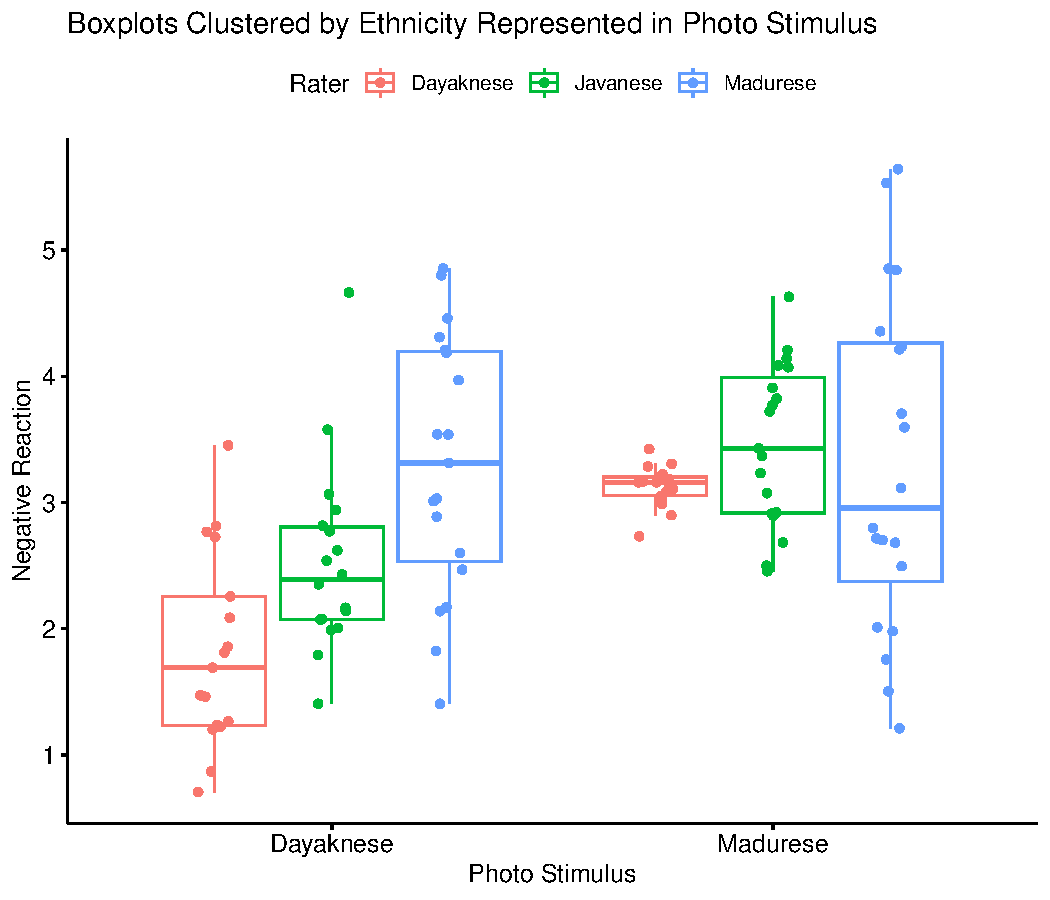
\includegraphics{04-tOneSample_files/figure-latex/unnamed-chunk-11-1.pdf} We can also obtain the probability value with the \emph{pnorm()} function. We enter the score, the mean, and the standard deviation. As shown below, we can enter them in \emph{z} score formula or from the raw scores.

\begin{Shaded}
\begin{Highlighting}[]
\FunctionTok{pnorm}\NormalTok{(}\DecValTok{0}\NormalTok{, }\AttributeTok{mean =} \DecValTok{0}\NormalTok{, }\AttributeTok{sd =} \DecValTok{1}\NormalTok{)}
\end{Highlighting}
\end{Shaded}

\begin{verbatim}
[1] 0.5
\end{verbatim}

\begin{Shaded}
\begin{Highlighting}[]
\FunctionTok{pnorm}\NormalTok{(}\FloatTok{9.9}\NormalTok{, }\AttributeTok{mean =} \FloatTok{9.9}\NormalTok{, }\AttributeTok{sd =} \DecValTok{2}\NormalTok{)}
\end{Highlighting}
\end{Shaded}

\begin{verbatim}
[1] 0.5
\end{verbatim}

Next, let's ask a question that requires careful inspection of the asymmetry of the curve. What is the probability that a physician spends less than 5 minutes with a patient? First, we calculate the corresponding \emph{z}-score:

\begin{Shaded}
\begin{Highlighting}[]
\CommentTok{\# calculating the z{-}score}
\NormalTok{(}\DecValTok{5} \SpecialCharTok{{-}} \FloatTok{9.9}\NormalTok{)}\SpecialCharTok{/}\DecValTok{2}  \CommentTok{\#for 5 minutes}
\end{Highlighting}
\end{Shaded}

\begin{verbatim}
[1] -2.45
\end{verbatim}

Second we locate the corresponding area under the normal curve. Examining the table of critical \emph{z}-values we see that a \emph{z}-score of -2.45 corresponds with an area of 0.0071. We can check this with the \emph{pnorm()} function:

\begin{Shaded}
\begin{Highlighting}[]
\FunctionTok{pnorm}\NormalTok{(}\SpecialCharTok{{-}}\FloatTok{2.45}\NormalTok{, }\AttributeTok{mean =} \DecValTok{0}\NormalTok{, }\AttributeTok{sd =} \DecValTok{1}\NormalTok{)  }\CommentTok{\#using SD or standardized units}
\end{Highlighting}
\end{Shaded}

\begin{verbatim}
[1] 0.007142811
\end{verbatim}

\begin{Shaded}
\begin{Highlighting}[]
\FunctionTok{pnorm}\NormalTok{(}\DecValTok{5}\NormalTok{, }\AttributeTok{mean =} \FloatTok{9.9}\NormalTok{, }\AttributeTok{sd =} \DecValTok{2}\NormalTok{)  }\CommentTok{\#using raw data units}
\end{Highlighting}
\end{Shaded}

\begin{verbatim}
[1] 0.007142811
\end{verbatim}

\includegraphics{04-tOneSample_files/figure-latex/unnamed-chunk-15-1.pdf} There is a .7\% (that is less than 1\%) probability that physicians spend less than 5 minutes with a patient. The inverse (1 - .7) indicates that we can be 99\% confident that patients receive 5 or more minutes with the ICU physician.

What about operations at the other end of the curve? What is the probability that a patient receives less than 12 minutes with a physician? Again, we start with the calculation of the \emph{z}-score.

\begin{Shaded}
\begin{Highlighting}[]
\NormalTok{(}\DecValTok{12} \SpecialCharTok{{-}} \FloatTok{9.9}\NormalTok{)}\SpecialCharTok{/}\DecValTok{2}  \CommentTok{\#for 12 minutes}
\end{Highlighting}
\end{Shaded}

\begin{verbatim}
[1] 1.05
\end{verbatim}

The 12 minute mark is 1.05 \emph{SD} above the mean. Checking the \emph{z} table lets us know that an area of 0.8531 corresponds with a \emph{z}-score of 1.05.

\begin{Shaded}
\begin{Highlighting}[]
\DecValTok{1}\FloatTok{{-}.8531}
\end{Highlighting}
\end{Shaded}

\begin{verbatim}
[1] 0.1469
\end{verbatim}

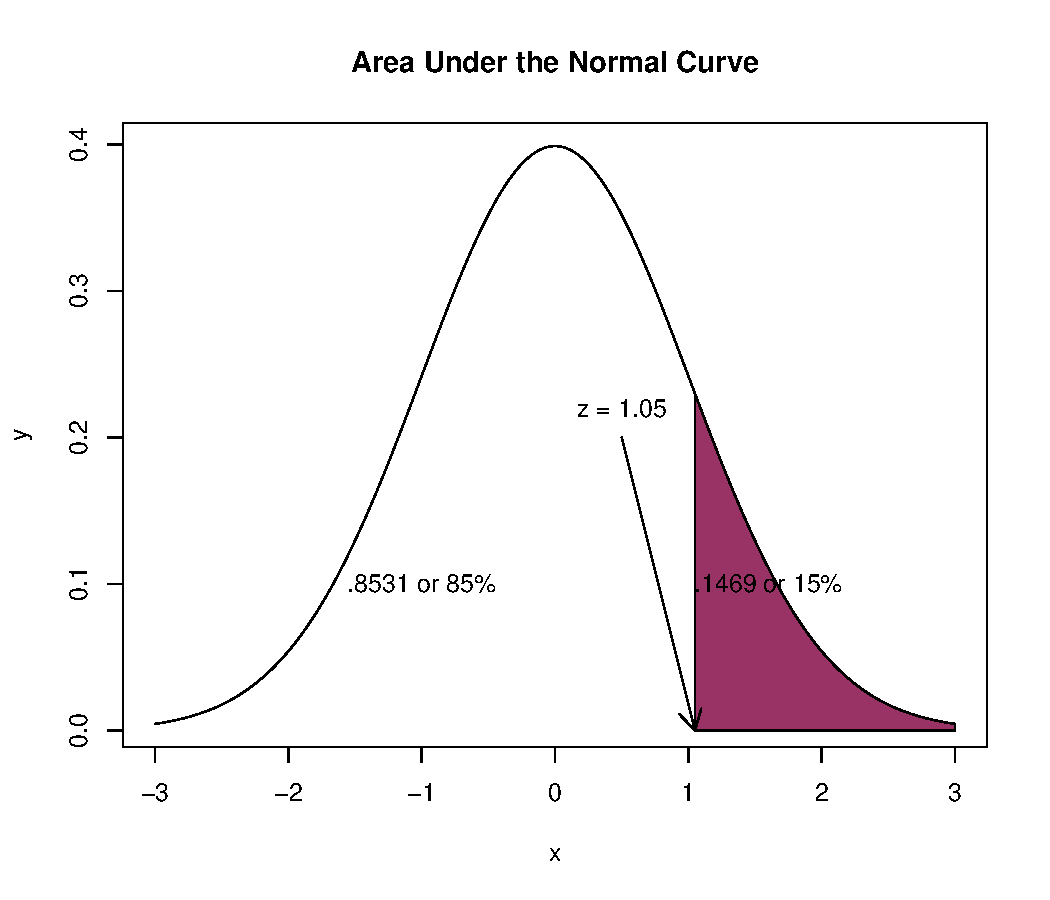
\includegraphics{04-tOneSample_files/figure-latex/unnamed-chunk-18-1.pdf} The probability of a physician spending 12 minutes \emph{or less} with a patient is 85\%; the probability of a physician spending 12 minutes or more with a patient is 15\%.

\hypertarget{percentiles}{%
\subsection{Percentiles}\label{percentiles}}

The same values that we just collected are often interpreted as percentiles. Our prior calculations taught us that a physician/patient visit that lasted 9.9 minutes (\emph{z} = 0), is ranked at the 50th percentile. That is, a 9.9 minute visit is longer than 50\% of patient/physician visits.

A visit lasting 5 minutes (\emph{z} = -2.45) is ranked at the .07th percentile. That is fewer than 1\% of patient/physician visits are shorter than 5 minutes.

Finally, a visit lasting 12 minutes (\emph{z} = 1.05) is ranked at the 85th percentile. That is, it is longer than 85\% of patient visits.

While this seems redundant, this something of a prelude to the importance of \emph{z} scores and the standard normal curve in assessment, evaluation, and psychometrics.

\hypertarget{transforming-variables-to-standard-scores}{%
\subsection{Transforming Variables to Standard Scores}\label{transforming-variables-to-standard-scores}}

At this point, we have hand-calculated each score. It is easy to transform a set of scores into a column of \emph{z}-scores:

\begin{Shaded}
\begin{Highlighting}[]
\NormalTok{PhysTime}\SpecialCharTok{$}\NormalTok{zMinutes }\OtherTok{\textless{}{-}}\NormalTok{ (PhysTime}\SpecialCharTok{$}\NormalTok{minutes }\SpecialCharTok{{-}} \FunctionTok{mean}\NormalTok{(PhysTime}\SpecialCharTok{$}\NormalTok{minutes))}\SpecialCharTok{/}\FunctionTok{sd}\NormalTok{(PhysTime}\SpecialCharTok{$}\NormalTok{minutes)}

\FunctionTok{head}\NormalTok{(PhysTime)}
\end{Highlighting}
\end{Shaded}

\begin{verbatim}
    minutes    zMinutes
1 10.300602  0.20226980
2 10.143081  0.12370440
3  9.785452 -0.05466684
4 13.162710  1.62977447
5  6.120944 -1.88237678
6 11.793346  0.94679063
\end{verbatim}

The transformation of scores is considered to be \emph{linear}. That is, this 1:1 relationship would result in a correlation of 1.00. Further, the \emph{z}-version of the variable could be used in analyses, just as the original raw score. Choices to do this are made carefully and usually done to optimize interpretation. I will demonstrate this with set of descriptive statistics produced by the \emph{apa.cor.table()} function from the \emph{apaTables} package.

\begin{Shaded}
\begin{Highlighting}[]
\NormalTok{apaTables}\SpecialCharTok{::}\FunctionTok{apa.cor.table}\NormalTok{(PhysTime)}
\end{Highlighting}
\end{Shaded}

\begin{verbatim}


Means, standard deviations, and correlations with confidence intervals
 

  Variable    M    SD   1           
  1. minutes  9.90 2.00             
                                    
  2. zMinutes 0.00 1.00 1.00**      
                        [1.00, 1.00]
                                    

Note. M and SD are used to represent mean and standard deviation, respectively.
Values in square brackets indicate the 95% confidence interval.
The confidence interval is a plausible range of population correlations 
that could have caused the sample correlation (Cumming, 2014).
 * indicates p < .05. ** indicates p < .01.
 
\end{verbatim}

\hypertarget{the-one-sample-z-test}{%
\subsection{\texorpdfstring{The One-Sample \emph{z} test}{The One-Sample z test}}\label{the-one-sample-z-test}}

The one-sample \emph{z} test is a common entry point to hypothesis testing. Let's imagine that we have reason to believe that an optimal physician/patient interaction in the ICU is 10.5 minutes. We want to use this value as a contrast to our own data and ask if the physician/patient interactions in our ICU are statistically significantly different. To test this hypothesis, we first set up null (\(H_0\)) and alternative (\(H_A\)) hypotheses. Our null hypothesis states that the population mean for physician/patient visits is equal to 10.5; the alternative hypothesis states that it is unequal to 10.5.

As written, this question is \emph{two-tailed.} That is, the external mean could be larger or smaller, we are just curious to see if it is different.

\[
\begin{array}{ll}
H_0: & \mu = 10.5 \\
H_A: & \mu \neq 10.5
\end{array}
\] Alternatively, we could ask a \emph{one-sided} question. That is, we might hypothesize that our sample mean is smaller than the external mean.

\[
\begin{array}{ll}
H_0: & \mu = 10.5 \\
H_A: & \mu < 10.5
\end{array}
\] Whether the test is one- or two- sided makes a difference in the strictness with which we interpret the results and can impact whether or not the result is statistically significant. We will reject the \(H_0\) in favor of the alternative (\(H_A\)) if the resulting test statistic (a \emph{z} score) falls into the region of rejection (but that region shifts, depending on whether our test is one- or two- tailed).

Statistician, Sir Ronald Fisher, popularized 5\% as the region of rejection. Specifically, if a probability value associated with a \emph{z}-score (or similar) falls into the tails of a distribution that represent 5\%, then the \(H_0\) is rejected, in favor of the \(H_A\).

Stated another way

\begin{itemize}
\tightlist
\item
  \emph{p} is the probability that the \(H_0\) is true

  \begin{itemize}
  \tightlist
  \item
    \emph{p} \textgreater{} 0.05 suggests that there is a 95\% chance or greater that the \(H_0\) is true
  \end{itemize}
\item
  1 minus the \emph{p} value is the probability that the alternative hypothesis is true.

  \begin{itemize}
  \tightlist
  \item
    A statistically significant test result (\emph{p} \textless{} 0.05) means that the test hypothesis is false or should be rejected.
  \item
    A \emph{p} value greater than 0.05 means that no effect was observed.
  \end{itemize}
\end{itemize}

If our hypothesis is two-sided, then we can spread the 5\% across both tails of the test. Inspecting a table of \emph{z} values shows that \(\pm 1.96\) would be the region of rejection of \(H_0\). In contrast, if the hypothesis is directionless (two-tailed), \(1.64\) would serve as the boundary for the region of rejection and the corresponding \emph{z}-test would require the same sign (+ or -) as the hypothesized tail of the distribution. So long as the hypothesis is consistent with the data, a one-sided test can be more powerful, that is, there is greater probability (defined as area under the curve) for rejecting the \(H_0\), if it is should be rejected. 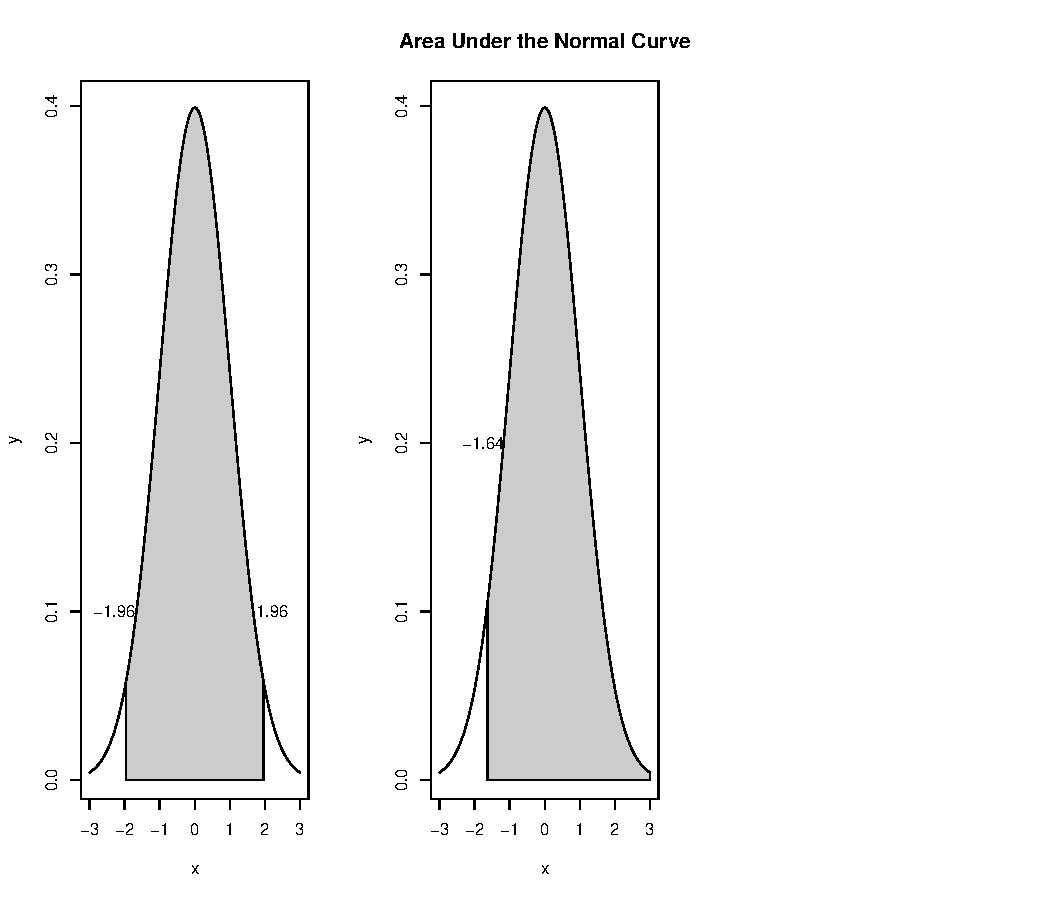
\includegraphics{04-tOneSample_files/figure-latex/unnamed-chunk-21-1.pdf}

The formula for a one-sample \emph{z}-test is as follows:

\[
z_{\bar{X}} =  \frac{\bar{X} - \mu_0}{\sigma / \sqrt{N}}
\] We have already calculated these values. But let's calculate some of them again as a reminder:

\begin{Shaded}
\begin{Highlighting}[]
\NormalTok{psych}\SpecialCharTok{::}\FunctionTok{describe}\NormalTok{(PhysTime}\SpecialCharTok{$}\NormalTok{minutes)}
\end{Highlighting}
\end{Shaded}

\begin{verbatim}
   vars   n mean sd median trimmed mad  min   max range skew kurtosis   se
X1    1 200  9.9  2   9.98    9.93   2 3.68 15.15 11.47 -0.2     0.03 0.14
\end{verbatim}

\begin{itemize}
\tightlist
\item
  Sample mean is 9.9
\item
  Population mean (the one we're comparing to) is 10.5
\item
  Standard deviation is 2
\item
  \emph{N} is 200
\end{itemize}

\begin{Shaded}
\begin{Highlighting}[]
\NormalTok{(}\FloatTok{9.9} \SpecialCharTok{{-}} \FloatTok{10.5}\NormalTok{)}\SpecialCharTok{/}\NormalTok{(}\DecValTok{2}\SpecialCharTok{/}\FunctionTok{sqrt}\NormalTok{(}\DecValTok{200}\NormalTok{))}
\end{Highlighting}
\end{Shaded}

\begin{verbatim}
[1] -4.242641
\end{verbatim}

The resulting value, \(z = -4.242\) is our test value. Because this far exceeds \(\pm 1.96\) we know (from memory) that there is a statistically significant effect. Just to be certain, let's use the \emph{pnorm()} function to obtain the \emph{p} value.

\begin{Shaded}
\begin{Highlighting}[]
\FunctionTok{pnorm}\NormalTok{(}\SpecialCharTok{{-}}\FloatTok{4.24}\NormalTok{, }\AttributeTok{mean =} \FloatTok{9.9}\NormalTok{, }\AttributeTok{sd =} \DecValTok{2}\NormalTok{)}
\end{Highlighting}
\end{Shaded}

\begin{verbatim}
[1] 0.0000000000007746685
\end{verbatim}

Simply with these hand-calculations, we can claim that there was a statistically significant difference between the physician/patient visit times in our simulated sample data and external benchmark criteria: \(z(200) = -4.24, p < .001\).

The one sample \emph{z}-test is rarely sighted in the published literature. However, a close inspection of a table of critical \emph{t}-values, reveals that the very bottom row (i.e., when sample sizes are 120 or greater) is, in fact, the \emph{z} criteria. Thus, it is time to learn about the one sample \emph{t}-test.

\hypertarget{introducing-the-one-sample-t-test}{%
\section{\texorpdfstring{Introducing the One-Sample \emph{t}-test}{Introducing the One-Sample t-test}}\label{introducing-the-one-sample-t-test}}

The one-sample \emph{t}-test is used to evaluate whether the mean of a sample differs from another value that, symbolically, is represented as the population mean. Green and Salkind \citeyearpar{green_using_2017} noted that this value is often the midpoint of set of scores, the average value of the test variable based on past research, or a test value as the chance level of performance.

\begin{figure}
\centering

\includegraphics{images/ttests/onesample.jpg}
\caption{An image of a row with two boxes labeled Condition A (in light blue) and the population mean (in dark blue) to which it is being compared. This represents the use of a one-sample \emph{t}-test.}
\end{figure}

This comparison is evident in the numerator of the formula for the \emph{t}-test that shows the population mean \(\mu\) being subtracted from the sample mean\(\bar{X}\).

\[
t = \frac{\bar{X} - \mu}{\hat{\sigma}/\sqrt{N} }
\] Although this statistic is straightforward, it is quite limited. If the researcher wants to compare an outcome variable across two groups of people, they should consider the \protect\hyperlink{tIndSample}{independent samples \emph{t}-test}. If the participant wants to evaluate an outcome variable with two observations from the same group of people, they should consider the \protect\hyperlink{tPaired}{paired samples \emph{t}-test}

\hypertarget{workflow-for-the-one-sample-t-test}{%
\subsection{\texorpdfstring{Workflow for the One-Sample \emph{t}-test}{Workflow for the One-Sample t-test}}\label{workflow-for-the-one-sample-t-test}}

The following is a proposed workflow for conducting a one-sample \emph{t}-test.

\begin{figure}
\centering
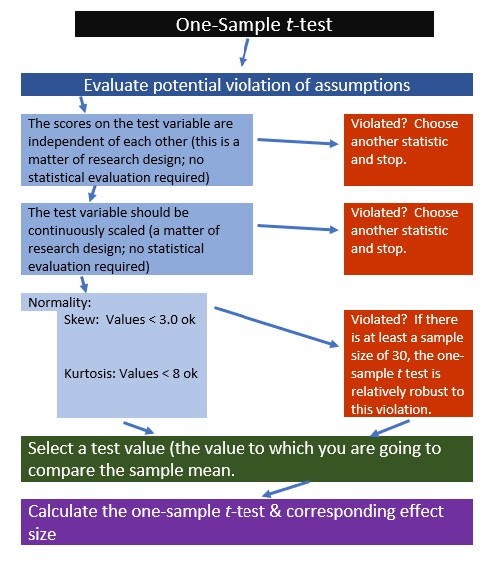
\includegraphics{images/ttests/OneSampleWrkFlw.jpg}
\caption{A colorful image of a workflow for the one sample \emph{t}-test}
\end{figure}

If the data meets the assumptions associated with the research design (e.g., independence of observations and a continuously scaled metric), these are the steps for the analysis of a one-sample \emph{t}-test:

\begin{enumerate}
\def\labelenumi{\arabic{enumi}.}
\tightlist
\item
  Prepare (upload) data.
\item
  Explore data with

  \begin{itemize}
  \tightlist
  \item
    graphs
  \item
    descriptive statistics
  \end{itemize}
\item
  Assess normality via skew and kurtosis
\item
  Select the comparison (i.e., test, population) value
\item
  Compute the one sample \emph{t}-test
\item
  Compute an effect size (frequently the \emph{d} statistic)
\item
  Manage Type I error
\item
  Sample size/power analysis (which you should think about first, but in the context of teaching statistics, it's more pedagogically sensible, here).
\end{enumerate}

\hypertarget{research-vignette-1}{%
\section{Research Vignette}\label{research-vignette-1}}

Empirically published articles where \emph{t}-tests are the primary statistic are difficult to locate. Having exhausted the psychology archives, I located this article in an interdisciplinary journal focused on palliative medicine. The research vignette for this lesson examined differences in physician's verbal and nonverbal communication with Black and White patients at the end of life \citep{elliott_differences_2016}.

Elliott and colleagues \citeyearpar{elliott_differences_2016} were curious to know if hospital-based physicians (56\% White, 26\% Asian, 7.4\% each Black and Hispanic) engaged in verbal and nonverbal communication differently with Black and White patients. Black and White patient participants were matched on characteristics deemed important to the researchers (e.g., critically and terminally ill, prognostically similar, expressed similar treatment preferences). Interactions in the intensive care unit were audio and video recorded and then coded on dimensions of verbal and nonverbal communication.

Because each physician saw a pair of patients (i.e., one Black patient and one White patient), the researchers utilized a paired samples, or dependent \emph{t}-test. This statistical choice was consistent with the element of the research design that controlled for physician effects through matching (and one we will work in a later lesson). Below are the primary findings of the study.

\begin{longtable}[]{@{}llll@{}}
\toprule\noalign{}
& Black Patients & White Patients & \\
\midrule\noalign{}
\endhead
\bottomrule\noalign{}
\endlastfoot
Category & \emph{Mean}(\emph{SD}) & \emph{Mean}(\emph{SD}) & \emph{p}-value \\
Verbal skill score (range 0 - 27) & 8.37(3.36) & 8.41(3.21) & 0.958 \\
Nonverbal skill score (range 0 - 5) & 2.68(.84) & 2.93(.77) & 0.014 \\
\end{longtable}

In the research vignette Elliott et al. \citeyearpar{elliott_differences_2016} indicated that physician/patient visits lasted between 3 minutes and 40 seconds to 20 minutes and 13 seconds. For the purpose of demonstrating the one sample \emph{t}-test, we might want to ask whether the length of patient visits in this research study were statistically significantly different than patient in the ICU or in palliative care, more broadly. Elliott et al.\citeyearpar{elliott_differences_2016} did not indicate a measure of central tendency (i.e., mean, mode, median) therefore, I will simulate the data by randomly generating 33 numbers with a mean of 8 and a standard deviation of 2.5. I will use \emph{random selection with replacement}, which allows the same number to be selected more than once.

\hypertarget{data-simulation}{%
\subsection{Data Simulation}\label{data-simulation}}

I re-simulated (what may seem like identical data from above)to be consistent with the journal article's research sample of 33.

\begin{Shaded}
\begin{Highlighting}[]
\CommentTok{\# Setting the \textquotesingle{}random\textquotesingle{} seed ensures that everyone gets the same}
\CommentTok{\# result, every time they rerun the analysis. My personal practice is}
\CommentTok{\# to create a random seed that represents the day I write up the}
\CommentTok{\# problem (in this case August, 15, 2022) When the Suggestions for}
\CommentTok{\# Practice invite you to \textquotesingle{}change the random seed,\textquotesingle{} simply change this}
\CommentTok{\# number to anything you like (maybe your birthday or today\textquotesingle{}s date)}
\FunctionTok{set.seed}\NormalTok{(}\DecValTok{220822}\NormalTok{)}
\NormalTok{dfOneSample }\OtherTok{\textless{}{-}} \FunctionTok{data.frame}\NormalTok{(}\AttributeTok{PhysMins =} \FunctionTok{rnorm}\NormalTok{(}\DecValTok{33}\NormalTok{, }\AttributeTok{mean =} \DecValTok{10}\NormalTok{, }\AttributeTok{sd =} \FloatTok{2.5}\NormalTok{))}

\FunctionTok{head}\NormalTok{(dfOneSample)}
\end{Highlighting}
\end{Shaded}

\begin{verbatim}
   PhysMins
1  9.097343
2 11.385558
3  8.424395
4  8.640534
5 12.583856
6  8.949883
\end{verbatim}

A warning: this particularly analysis (the whole lesson, in fact) is ``more simulated than usual'' and does not represent reality. However, this research vignette lends itself for this type of question.

With our data in hand, let's examine its structure. The variable representing physician minutes represents the ratio scale of measurement and therefore should be noted as \emph{num} (numerical) in R.

\begin{Shaded}
\begin{Highlighting}[]
\FunctionTok{str}\NormalTok{(dfOneSample)}
\end{Highlighting}
\end{Shaded}

\begin{verbatim}
'data.frame':   33 obs. of  1 variable:
 $ PhysMins: num  9.1 11.39 8.42 8.64 12.58 ...
\end{verbatim}

Below is code for saving the data to your computer (and then re-importing) as .csv or .rds files. I make choices about saving data based on what I wish to do with the data. If I want to manipulate the data outside of R, I will save it as a .csv file. It is easy to open .csv files in Excel. A limitation of the .csv format is that it does not save any restructuring or reformatting of variables. For this lesson, this is not an issue.

Although you do not need to save nor re-import the data for this lesson, here is code for saving the data as a .csv and then reading it back into R. I have hashtagged these out, so you will need to remove the hashtags if you wish to run any of these operations.

\begin{Shaded}
\begin{Highlighting}[]
\CommentTok{\# writing the simulated data as a .csv write.table(dfOneSample, file}
\CommentTok{\# = \textquotesingle{}dfOneSample.csv\textquotesingle{}, sep = \textquotesingle{},\textquotesingle{}, col.names=TRUE, row.names=FALSE) at}
\CommentTok{\# this point you could clear your environment and then bring the data}
\CommentTok{\# back in as a .csv reading the data back in as a .csv file}
\CommentTok{\# dfOneSample\textless{}{-} read.csv (\textquotesingle{}dfOneSample.csv\textquotesingle{}, header = TRUE)}
\end{Highlighting}
\end{Shaded}

The .rds form of saving variables preserves any formatting (e.g., creating ordered factors) of the data. A limitation is that these files are not easily opened in Excel. Again, you do not need to save nor re-import the data for this lesson. However, if you would like to do so, here is the hashtagged code (remove hashtags if you wish to do this) for writing (and then reading) this data as an .rds file.

\begin{Shaded}
\begin{Highlighting}[]
\CommentTok{\# saveRDS(dfOneSample, \textquotesingle{}dfOneSample.rds\textquotesingle{}) dfOneSample \textless{}{-}}
\CommentTok{\# readRDS(\textquotesingle{}dfOneSample.rds\textquotesingle{})}
\end{Highlighting}
\end{Shaded}

\hypertarget{quick-peek-at-the-data}{%
\subsection{Quick Peek at the Data}\label{quick-peek-at-the-data}}

Plotting the data is best practice to any data analysis. Further, visualizing the data can help us with a conceptual notion of the statistic we are utilizing. The \emph{ggpubr} package is one of my go-to-tools for quick and easy plots of data. Below, I have plotted the time-with-patient (Physician Seconds) variable and added the mean. As with most plotting packages, ggpubr will ``bin'' (or cluster) the data for plotting; this is especially true for data with a large number of units (a range from 220 to 1213 is quite large). The ``rug = TRUE'' command added a lower row of the table to identify where each of the datapoint follows.

\begin{Shaded}
\begin{Highlighting}[]
\NormalTok{ggpubr}\SpecialCharTok{::}\FunctionTok{gghistogram}\NormalTok{(dfOneSample, }\AttributeTok{x =} \StringTok{"PhysMins"}\NormalTok{, }\AttributeTok{add =} \StringTok{"mean"}\NormalTok{, }\AttributeTok{rug =} \ConstantTok{TRUE}\NormalTok{,}
    \AttributeTok{color =} \StringTok{"\#993366"}\NormalTok{)}
\end{Highlighting}
\end{Shaded}

\begin{verbatim}
Warning: Using `bins = 30` by default. Pick better value with the argument
`bins`.
\end{verbatim}

\begin{verbatim}
Warning: `geom_vline()`: Ignoring `mapping` because `xintercept` was provided.
\end{verbatim}

\begin{verbatim}
Warning: `geom_vline()`: Ignoring `data` because `xintercept` was provided.
\end{verbatim}

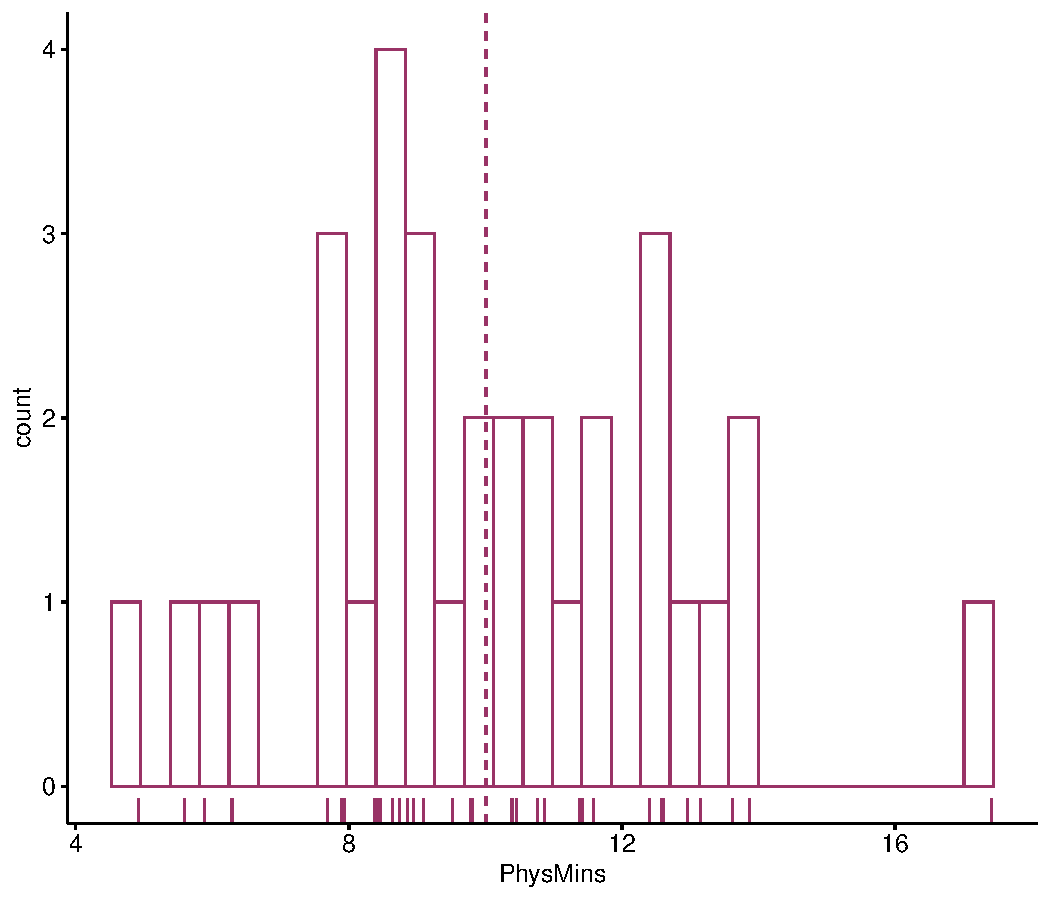
\includegraphics{04-tOneSample_files/figure-latex/unnamed-chunk-29-1.pdf}

Although the histogram is not perfectly normal, we can see at least the suggestion of a normal distribution. With only a sample of 33, I'm encouraged.

Another view of our data is with a boxplot. The box captures the middle 50\% of data with the horizontal bar at the median. The whiskers extend three standard deviations around the mean with dots beyond the whiskers representing outliers. I personally like the \emph{add=``jitter''} statement because it shows where each case falls.

\begin{Shaded}
\begin{Highlighting}[]
\NormalTok{ggpubr}\SpecialCharTok{::}\FunctionTok{ggboxplot}\NormalTok{(dfOneSample}\SpecialCharTok{$}\NormalTok{PhysMins, }\AttributeTok{ylab =} \StringTok{"Minutes with Patient"}\NormalTok{,}
    \AttributeTok{xlab =} \ConstantTok{FALSE}\NormalTok{, }\AttributeTok{add =} \StringTok{"jitter"}\NormalTok{)}
\end{Highlighting}
\end{Shaded}

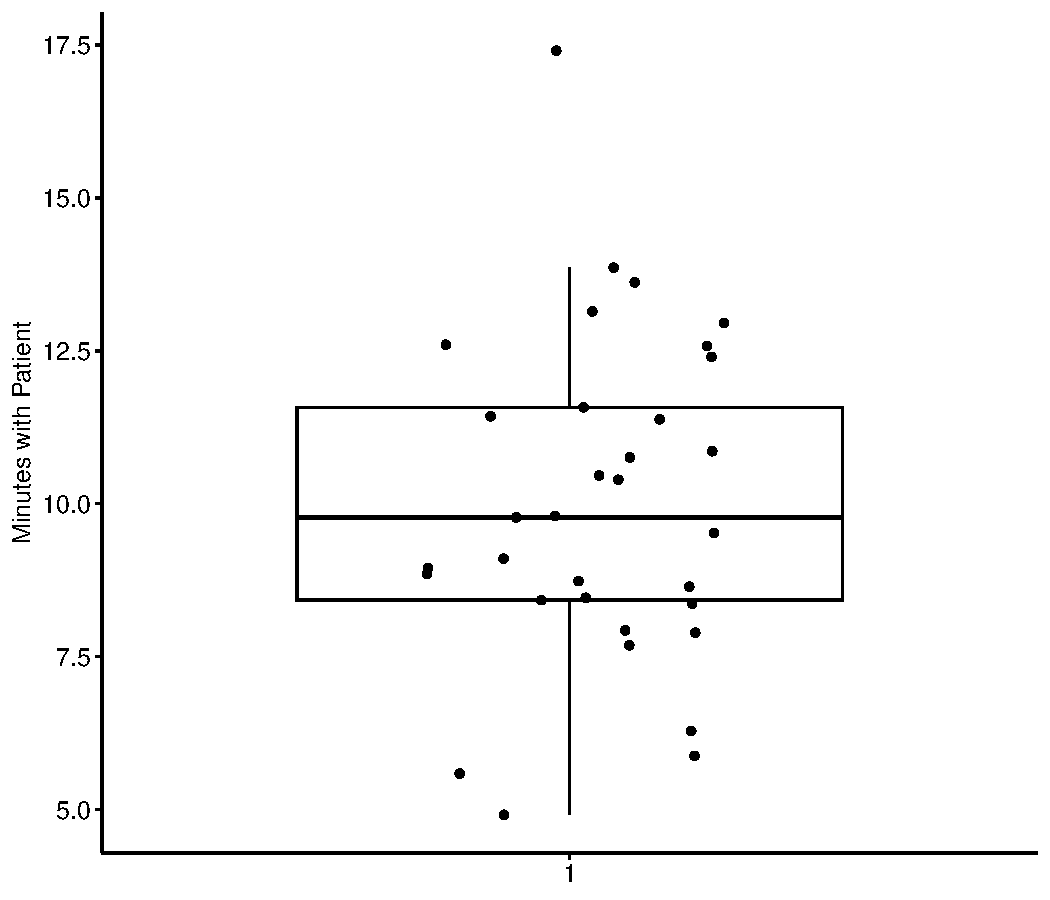
\includegraphics{04-tOneSample_files/figure-latex/unnamed-chunk-30-1.pdf} We can further evaluate normality by obtaining the descriptive statistics with the \emph{describe()} function from the \emph{psych} package.

\begin{Shaded}
\begin{Highlighting}[]
\NormalTok{psych}\SpecialCharTok{::}\FunctionTok{describe}\NormalTok{(dfOneSample}\SpecialCharTok{$}\NormalTok{PhysMins)}
\end{Highlighting}
\end{Shaded}

\begin{verbatim}
   vars  n  mean  sd median trimmed  mad  min   max range skew kurtosis   se
X1    1 33 10.01 2.7   9.78    9.96 2.44 4.92 17.41 12.49 0.36     0.04 0.47
\end{verbatim}

Here we see that our minutes range from 4.92 to 17.41 with a mean of 10.01 and a standard deviation of 2.7. We're ready to calculate the one sample \emph{t}-test.

\hypertarget{working-the-one-sample-t-test-by-hand}{%
\section{\texorpdfstring{Working the One Sample \emph{t}-test (by hand)}{Working the One Sample t-test (by hand)}}\label{working-the-one-sample-t-test-by-hand}}

\hypertarget{stating-the-hypothesis}{%
\subsection{Stating the Hypothesis}\label{stating-the-hypothesis}}

A quick scan of the literature suggests that health care workers' visits to patients in the ICU are typically quite brief. Specifically, the average duration of a physician visit in a 2018 study was 73.5 seconds or 1.23 minutes \citep{butler_estimating_2018}. A one-sample \emph{t}-test is appropriate for comparing the visit lengths from our sample to this external metric.

As noted in the symbolic presentation below, our null hypothesis (\(H_0\)) states that our data will be equal to the test value of 1.23 minutes. In contrast, the alternative hypothesis (\(H_A\)) states that these values will not be equal.

\[
\begin{array}{ll}
H_0: & \mu = 1.23 \\
H_A: & \mu \neq 1.23
\end{array}
\]

\hypertarget{calculating-the-t-test}{%
\subsection{\texorpdfstring{Calculating the \emph{t}-test}{Calculating the t-test}}\label{calculating-the-t-test}}

In learning the statistic, hand-calculations can help understand what the statistic is doing. Here's the formula again:

\[
t = \frac{\bar{X} - \mu}{\hat{\sigma}/\sqrt{N} }
\]

The numerator of the formula below subtracts the test value from the sample mean. The denominator involves multiplying the standard deviation by the square root of the sample size. The descriptive statistics provided the values we need to complete the analysis:

\begin{Shaded}
\begin{Highlighting}[]
\NormalTok{(}\FloatTok{10.01} \SpecialCharTok{{-}} \FloatTok{1.23}\NormalTok{)}\SpecialCharTok{/}\NormalTok{(}\FloatTok{2.7}\SpecialCharTok{/}\FunctionTok{sqrt}\NormalTok{(}\DecValTok{33}\NormalTok{))}
\end{Highlighting}
\end{Shaded}

\begin{verbatim}
[1] 18.68047
\end{verbatim}

\hypertarget{statistical-significance}{%
\subsubsection{Statistical Significance}\label{statistical-significance}}

If we ask about \emph{statistical significance} then we are engaged in \emph{null hypothesis significance testing} (NHST). In the case of a one sample test, we construct our hypothesis with a null and an alternative that are relatively straightforward. Specifically, we are interested in knowing if our sample mean (10.01) is statistically, significantly different from the test value of 1.23. We can write the hypotheses in this way:

\[
\begin{array}{ll}
H_0: & \mu = 1.23 \\
H_A: & \mu \neq 1.23
\end{array}
\] In two parts, our null hypothesis (\(H_0\)) states that the population mean (\(H_0\)) for physician visits with palliative care patients is 1.23; the alternative \(\mu \neq\) states that it is not 1.23.

When we calculated the \emph{t}-test, we obtained a \emph{t} value. We can check the statistical significance by determining the test critical value from a \href{https://www.statology.org/t-distribution-table/}{table of critical values} for the \emph{t} distribution. There are many freely available on the internet. If our \emph{t} value exceeds the value(s) in the table of critical values, then we can claim that our sample mean is statistically significantly different from the hypothesized value.

Heading to the table of critical values we do the following:

\begin{itemize}
\tightlist
\item
  For the one-sample \emph{t}-test, the degrees of freedom (DF) is equal to \emph{N} - 1 (32). The closest value in our table is 30, so we will use that row.
\item
  A priorily, we did not specify if we thought the difference would be greater, or lower. Therefore, we will use a column that indicates \emph{two-tails}.
\item
  A \emph{p} value of .05 is customary (but it will be split between two tails).
\item
  Thus, if our \emph{t}-value is lower than -2.042 or higher than 2.042 we know we have a statistically significant difference.
\end{itemize}

In our case, the \emph{t} value of 18.68 far exceeded the test critical value of 2.042. We would write the statistical string this way: \emph{t}(32) = 18.68, \emph{p} \textless{} .05.

In base R, the \emph{qt()} function will look up a test critical value. For the one-sample \emph{t}-test, degrees of freedom (df) is equal to \(N-1\). We ``divide the \emph{p} value by 2'' when we want a two-tailed test. Finally, the ``lower.tail'' command results in positive or negative values in the tail.

\begin{Shaded}
\begin{Highlighting}[]
\FunctionTok{qt}\NormalTok{(}\AttributeTok{p =} \FloatTok{0.05}\SpecialCharTok{/}\DecValTok{2}\NormalTok{, }\AttributeTok{df =} \DecValTok{32}\NormalTok{, }\AttributeTok{lower.tail =} \ConstantTok{FALSE}\NormalTok{)}
\end{Highlighting}
\end{Shaded}

\begin{verbatim}
[1] 2.036933
\end{verbatim}

Not surprisingly, this value is quite similar to the value we saw in the table. The \emph{qt()} function is more accurate because it used df = 32 (not rounded down to 30).

\hypertarget{confidence-intervals}{%
\subsubsection{Confidence Intervals}\label{confidence-intervals}}

How confident are we in our result? With the one sample \emph{t}-test, it is common to report an interval in which we are 95\% confident that that our sample mean exists. Below is the formula, which involves:

\begin{itemize}
\tightlist
\item
  \(\bar{X}\) is the sample mean; in our case this is 10.01
\item
  \(t_{cv}\) the test critical value for a two-tailed model (even if the hypothesis was one-tailed) where \(\alpha = .05\) and the degrees of freedom are \(N-1\)
\item
  \(\frac{s}{\sqrt{n}}\) was the denominator of the test statistic it involves the standard deviation of our sample (2.7) and the square root of our sample size (33)
\end{itemize}

\[\bar{X} \pm t_{cv}(\frac{s}{\sqrt{n}})\] Let's calculate it:

First, let's calculate the proper \emph{t} critical value. Even though these are identical to the one above, I am including them again. Why? Because if the original hypothesis had been one-tailed, we would need to calculate a two-tailed confidence interval; this is a placeholder to remind us.

\begin{Shaded}
\begin{Highlighting}[]
\FunctionTok{qt}\NormalTok{(}\AttributeTok{p =} \FloatTok{0.05}\SpecialCharTok{/}\DecValTok{2}\NormalTok{, }\AttributeTok{df =} \DecValTok{32}\NormalTok{, }\AttributeTok{lower.tail =} \ConstantTok{FALSE}\NormalTok{)}
\end{Highlighting}
\end{Shaded}

\begin{verbatim}
[1] 2.036933
\end{verbatim}

Using the values from above, we can specify both the lower and upper bound of our confidence interval.

\begin{Shaded}
\begin{Highlighting}[]
\NormalTok{(}\FloatTok{10.01}\NormalTok{) }\SpecialCharTok{{-}}\NormalTok{ ((}\FloatTok{2.0369}\NormalTok{) }\SpecialCharTok{*}\NormalTok{ (}\FloatTok{2.7}\SpecialCharTok{/}\FunctionTok{sqrt}\NormalTok{(}\DecValTok{33}\NormalTok{)))}
\end{Highlighting}
\end{Shaded}

\begin{verbatim}
[1] 9.052637
\end{verbatim}

\begin{Shaded}
\begin{Highlighting}[]
\NormalTok{(}\FloatTok{10.01}\NormalTok{) }\SpecialCharTok{+}\NormalTok{ ((}\FloatTok{2.0369}\NormalTok{) }\SpecialCharTok{*}\NormalTok{ (}\FloatTok{2.7}\SpecialCharTok{/}\FunctionTok{sqrt}\NormalTok{(}\DecValTok{33}\NormalTok{)))}
\end{Highlighting}
\end{Shaded}

\begin{verbatim}
[1] 10.96736
\end{verbatim}

The resulting interval is the 95\% confidence interval around our sample mean. Stated another way, we are 95\% certain that the true mean of time with patients in our sample ranges between 9.05 and 10.97 minutes.

\hypertarget{effect-size}{%
\subsubsection{Effect size}\label{effect-size}}

If you have heard someone say something like, ``I see there is statistical significance, but is the difference \emph{clinically significant},'' the person is probably asking about \emph{effect sizes.} Effect sizes provide an indication of the magnitude of the difference.

The \emph{d} statistic is commonly used with \emph{t}-tests; \emph{d} assesses the degree that the mean on the test variable differs from the test value. Conveniently, \emph{d} represents standard deviation units. A \emph{d} value of 0 indicates that the mean of the sample equals the mean of the test value. As \emph{d} moves away from 0 (in either direction), we can interpret the effect size to be stronger. Conventionally, the absolute values of .2, .5, and .8, represent small, medium, and large effect sizes, respectfully.

Calculating the \emph{d} statistic is easy. Here are two equivalent formulas:

\[d = \frac{Mean Difference}{SD}=\frac{t}{\sqrt{N}}\]

\begin{Shaded}
\begin{Highlighting}[]
\CommentTok{\# First formula}
\NormalTok{(}\FloatTok{10.01} \SpecialCharTok{{-}} \FloatTok{1.23}\NormalTok{)}\SpecialCharTok{/}\FloatTok{2.7}
\end{Highlighting}
\end{Shaded}

\begin{verbatim}
[1] 3.251852
\end{verbatim}

\begin{Shaded}
\begin{Highlighting}[]
\CommentTok{\# Second formula}
\FloatTok{18.68047}\SpecialCharTok{/}\FunctionTok{sqrt}\NormalTok{(}\DecValTok{33}\NormalTok{)}
\end{Highlighting}
\end{Shaded}

\begin{verbatim}
[1] 3.251852
\end{verbatim}

The value of 3.25 indicates that the test value is approximately more than three standard deviations away from the sample mean. This is a very large difference.

\hypertarget{working-the-one-sample-t-test-with-r-packages}{%
\section{\texorpdfstring{Working the One-Sample \emph{t}-test with R Packages}{Working the One-Sample t-test with R Packages}}\label{working-the-one-sample-t-test-with-r-packages}}

\hypertarget{evaluating-the-statistical-assumptions}{%
\subsection{Evaluating the Statistical Assumptions}\label{evaluating-the-statistical-assumptions}}

Let's rework the problem in R. We start at the top of the flowchart, evaluating the statistical assumptions.

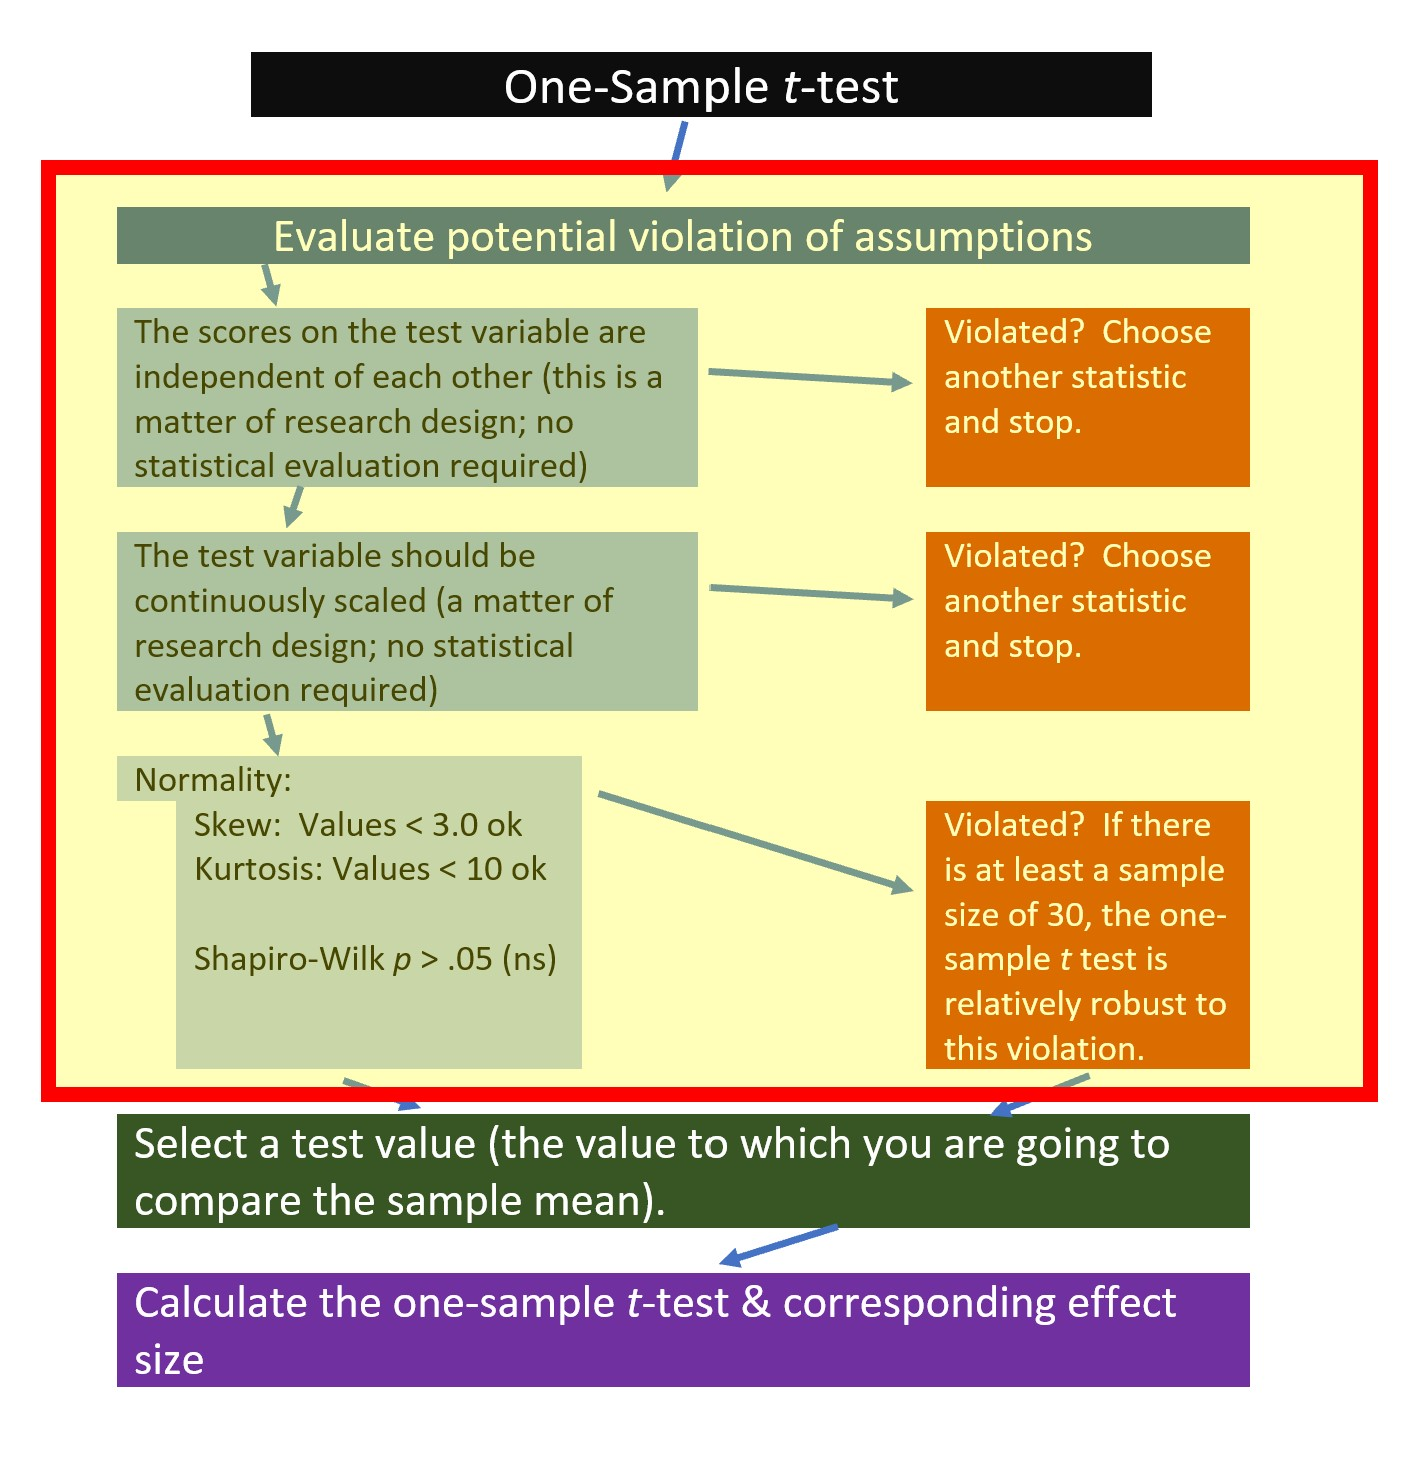
\includegraphics{images/ttests/OneSampleAssmptns.jpg} All statistical tests have some assumptions about the data. The one-sample \emph{t}-test has three.

\begin{itemize}
\tightlist
\item
  The scores on the test variable as independent of each other. This is a research design issue and the one-sample \emph{t}-test is not robust to violating this assumption.

  \begin{itemize}
  \tightlist
  \item
    If physicians were contributing more than one data point, this vignette potentially violated this assumption. For the sake of simplicity, let's presume that each physician contributed visit length (minutes) for only one patient. If the research scenario was such that physicians contributed multiple datapoints a potential analytic choice that is robust to such a violation is \href{https://lhbikos.github.io/MultilevelModeling/}{multilevel modeling}.
  \end{itemize}
\item
  The test variable should be continuously scaled. This is also a matter of research design and no statistical analysis is required.

  \begin{itemize}
  \tightlist
  \item
    Our test variable is measured in minutes; this is continuously scaled and has the properties of \emph{ratio}-level data.
  \end{itemize}
\item
  The test variable is normally distributed. We can check this several ways:

  \begin{itemize}
  \tightlist
  \item
    visually with histograms (perhaps with superimposed curves) and boxplots,
  \item
    calculation of skew and kurtosis values,
  \item
    calculation of the Shapiro-Wilk test of normality
  \end{itemize}
\end{itemize}

\hypertarget{is-the-test-variable-normally-distributed}{%
\subsubsection{Is the Test Variable Normally Distributed?}\label{is-the-test-variable-normally-distributed}}

Thus, we need only to assess whether the test variable is normally distributed. The \emph{pastecs::stat.desc()} function will provide all of this information in one test. We need only add the specification, ``norm=TRUE''.

\begin{Shaded}
\begin{Highlighting}[]
\CommentTok{\# pastecs is the package, stat.desc is the function we point it to}
\CommentTok{\# the data and then add the norm=TRUE command}
\NormalTok{pastecs}\SpecialCharTok{::}\FunctionTok{stat.desc}\NormalTok{(dfOneSample, }\AttributeTok{norm =} \ConstantTok{TRUE}\NormalTok{)}
\end{Highlighting}
\end{Shaded}

\begin{verbatim}
                 PhysMins
nbr.val       33.00000000
nbr.null       0.00000000
nbr.na         0.00000000
min            4.92123791
max           17.40834882
range         12.48711091
sum          330.26971365
median         9.77737813
mean          10.00817314
SE.mean        0.47011645
CI.mean.0.95   0.95759588
var            7.29331287
std.dev        2.70061342
coef.var       0.26984080
skewness       0.35985466
skew.2SE       0.44031259
kurtosis       0.03511647
kurt.2SE       0.02199140
normtest.W     0.97666915
normtest.p     0.68198838
\end{verbatim}

Recall from the lesson on \protect\hyperlink{preliminaries}{Preliminary Results} that there are multiple ways to assess severity of skew and kurtosis. Values greater than the absolute value of 3.0 are concerning for the ``skewness'' output. The PhysMins skewness values of 0.36 is well below that threshold. Values greater than the absolute value of 10 are concerning for the ``kurtosis'' output. The PhysMins skewness value of 0.035 is well below that thresshold. The ``skew.2SE'' and ``kurt.2SE'' values are standardized. The ``2'' in the ``skew.2SE'' is a helpful reminder that, in smaller sample sizes'', using the 1.96 (or ``2'') criteria is acceptable in determining problematic skew or kurtosis. The PhysMins values of 0.44 and 0.022 fall well below those areas of concern.

Regarding a formal assessment of normality, the \emph{pastecs::stat.descr()} output includes the Shapiro-Wilk value (normtest.W) and statistical significance (normtest.p). Non-significant results indicate that the distribution of the PhysMins variable is not statistically significantly different from a normal distribution. In the case of PhysMins, \(W = 0.977, p = 0.682\).

Considering skewness, kurtosis, and normality estimates together, we are confident that we have not violated the assumption of normality.

\hypertarget{computing-the-t-test}{%
\subsection{\texorpdfstring{Computing the \emph{t}-test}{Computing the t-test}}\label{computing-the-t-test}}

Now we are ready to calculate the \emph{t}-test, itself.

\begin{figure}
\centering
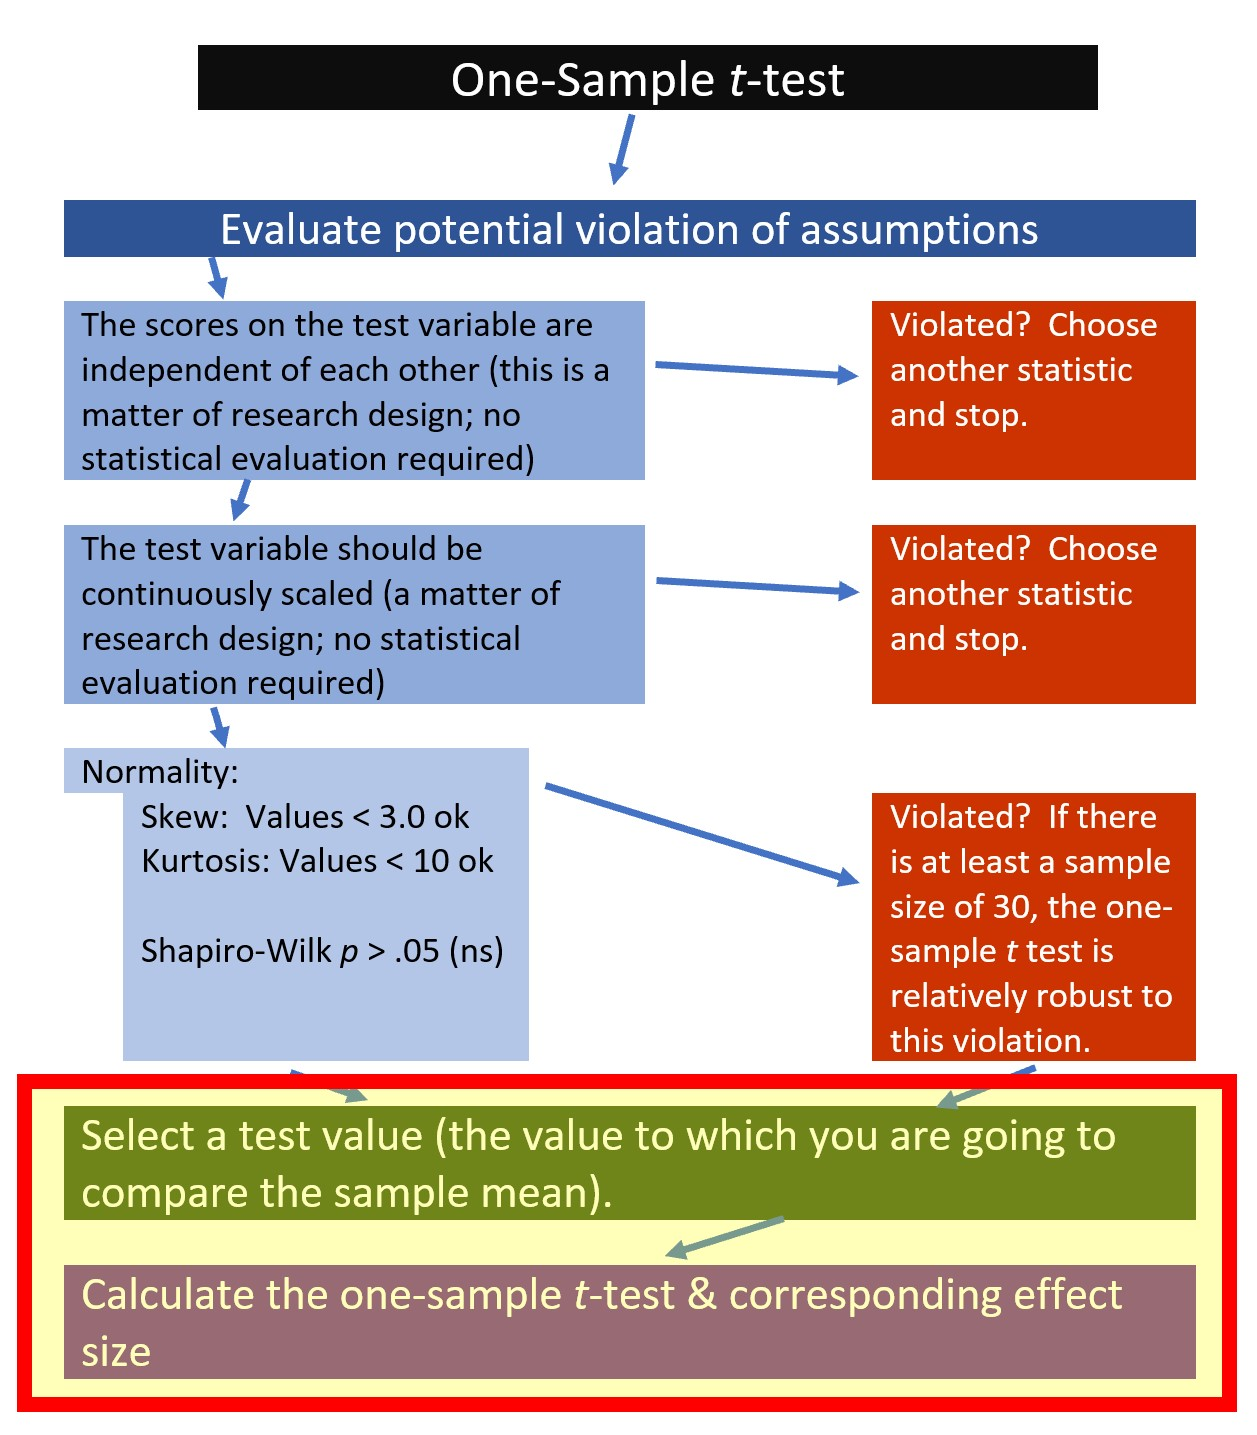
\includegraphics{images/ttests/OneSampleT.jpg}
\caption{The workflow for the one sample \emph{t}-test highlighting the evaluation of assumptions section}
\end{figure}

Calculating a one sample \emph{t}-test is possible through base R and a number of packages. Kassambara's \citeyearpar{kassambara_pipe-friendly_nodate} \emph{rstatix} package is one we can use for the \emph{t}-test and ANOVA problems that we will work. I like it for several reasons. First, it was designed to be ``pipe-friendly'' in a manner that is consistent with the \emph{tidyverse} approach to working in R and there are numerous tutorials. Additionally, \emph{rstatix} objects work well with \emph{ggpubr}, one of my favorite packages for graphing data and results.

In the script below:

\begin{itemize}
\tightlist
\item
  the first element points to the dataframe
\item
  the second element provides a ``formula''

  \begin{itemize}
  \tightlist
  \item
    we are predicting ``PhysMins'' from ``1'' which represent an invariant/constant hypothesized mean
  \end{itemize}
\item
  the third element identifies the population/comparison mean
\item
  specifying ``detailed = TRUE'' will produce the 95\% confidence interval around the mean (i.e., in this case the average amount of time that physicians in our sample spent with their patients)
\end{itemize}

\begin{Shaded}
\begin{Highlighting}[]
\NormalTok{rstatix}\SpecialCharTok{::}\FunctionTok{t\_test}\NormalTok{(dfOneSample, PhysMins }\SpecialCharTok{\textasciitilde{}} \DecValTok{1}\NormalTok{, }\AttributeTok{mu =} \FloatTok{1.23}\NormalTok{, }\AttributeTok{detailed =} \ConstantTok{TRUE}\NormalTok{)}
\end{Highlighting}
\end{Shaded}

\begin{verbatim}
# A tibble: 1 x 12
  estimate .y.   group1 group2     n statistic        p    df conf.low conf.high
*    <dbl> <chr> <chr>  <chr>  <int>     <dbl>    <dbl> <dbl>    <dbl>     <dbl>
1     10.0 Phys~ 1      null ~    33      18.7 9.07e-19    32     9.05      11.0
# i 2 more variables: method <chr>, alternative <chr>
\end{verbatim}

The results we obtained are identical to those we hand-calculated. The \emph{rstatix} output also includes confidence intervals. In the case of the one-sample \emph{t}-test, this represent the 95\% confidence interval around the mean. That is, we are 95\% confident that the true mean of the minutes that physicians in our sample spent with patients falls between 9.05 and 10.97. I appreciate that the \emph{rstatix} output reminds us that we are using a \emph{t}-test and that it is a two-sided hypothesis.

Knowing what the confidence interval is ``around'' can be tricky. Whatever the ``topic'' of the confidence interval will be exactly in the middle of (most) confidence intervals. We can check ourselves by adding the two ends of the confidence interval and dividing by two.

\begin{Shaded}
\begin{Highlighting}[]
\NormalTok{(}\FloatTok{9.050577} \SpecialCharTok{+} \FloatTok{10.96577}\NormalTok{)}\SpecialCharTok{/}\DecValTok{2}
\end{Highlighting}
\end{Shaded}

\begin{verbatim}
[1] 10.00817
\end{verbatim}

As we see, 10.008 is the reported as the ``estimate.'' We know from our earlier analysis of the descriptive statistics that this is the value of the mean. If we are uncertain, we can check:

\begin{Shaded}
\begin{Highlighting}[]
\FunctionTok{mean}\NormalTok{(dfOneSample}\SpecialCharTok{$}\NormalTok{PhysMins)}
\end{Highlighting}
\end{Shaded}

\begin{verbatim}
[1] 10.00817
\end{verbatim}

From these results, we can begin to create our \emph{t} string: \(t(32) = 18.67, p < .001, CI95(9.05, 10.97)\)

With a separate command, we can use the \emph{rstatix} package to obtain the effect size, \emph{d}. With the exception of including the ``ref.group = NULL'' statement, the script is quite similar.

\begin{Shaded}
\begin{Highlighting}[]
\NormalTok{rstatix}\SpecialCharTok{::}\FunctionTok{cohens\_d}\NormalTok{(dfOneSample, PhysMins }\SpecialCharTok{\textasciitilde{}} \DecValTok{1}\NormalTok{, }\AttributeTok{ref.group =} \ConstantTok{NULL}\NormalTok{, }\AttributeTok{mu =} \FloatTok{1.23}\NormalTok{)}
\end{Highlighting}
\end{Shaded}

\begin{verbatim}
# A tibble: 1 x 6
  .y.      group1 group2     effsize     n magnitude
* <chr>    <chr>  <chr>        <dbl> <int> <ord>    
1 PhysMins 1      null model    3.25    33 large    
\end{verbatim}

From these results, we can begin to complete our \emph{t} string: \(t(32) = 18.672, p < .001, CI95(9.05, 10.97), d = 3.25\)

\hypertarget{apa-style-results}{%
\section{APA Style Results}\label{apa-style-results}}

Let's write up the results. In-so-doing, I would include the boxplot we produced during our initial exploration of the data.

\begin{quote}
Preliminary inspection of the data indicated that we did not violate the assumption of normality. Specifically, our skew (0.36) and kurtosis (0.035) values fell below that absolute values (3.0, 10.0, respectively) that are concerning \citep{kline_data_2016}. Further, the Shapiro-Wilk test of normality suggested that the distribution of our sample data did not differ significantly from a normal distribution \((W = 0.977, p = 0.682)\)
\end{quote}

\begin{quote}
A one-sample \emph{t}-test was used to evaluate whether average amount of time that a sample of physicians (palliative care physicians in the ICU) enrolled in a research study on patient communication was statistically significantly different from the amount of time that ICU physicians spend with their patients, in general. The sample mean 10.008 (\emph{SD} = 2.7016) was significantly different from 1.23, \(t(32) = 18.672, p < .001., CI95(9.05, 10.97), d = 3.25\). The effect size, (\emph{d}) indicates a very large effect. Figure 1 illustrates the distribution of time physicians in the research study spent with their patients. The results support the conclusion that physicians in the research study spent more time with their patients than ICU physicians in general.
\end{quote}

\begin{Shaded}
\begin{Highlighting}[]
\NormalTok{ggpubr}\SpecialCharTok{::}\FunctionTok{ggboxplot}\NormalTok{(dfOneSample}\SpecialCharTok{$}\NormalTok{PhysMins, }\AttributeTok{ylab =} \StringTok{"Physician Minutes"}\NormalTok{, }\AttributeTok{xlab =} \ConstantTok{FALSE}\NormalTok{,}
    \AttributeTok{add =} \StringTok{"jitter"}\NormalTok{, }\AttributeTok{title =} \StringTok{"Figure 1. Physician Time with Patients (in minutes)"}\NormalTok{)}
\end{Highlighting}
\end{Shaded}

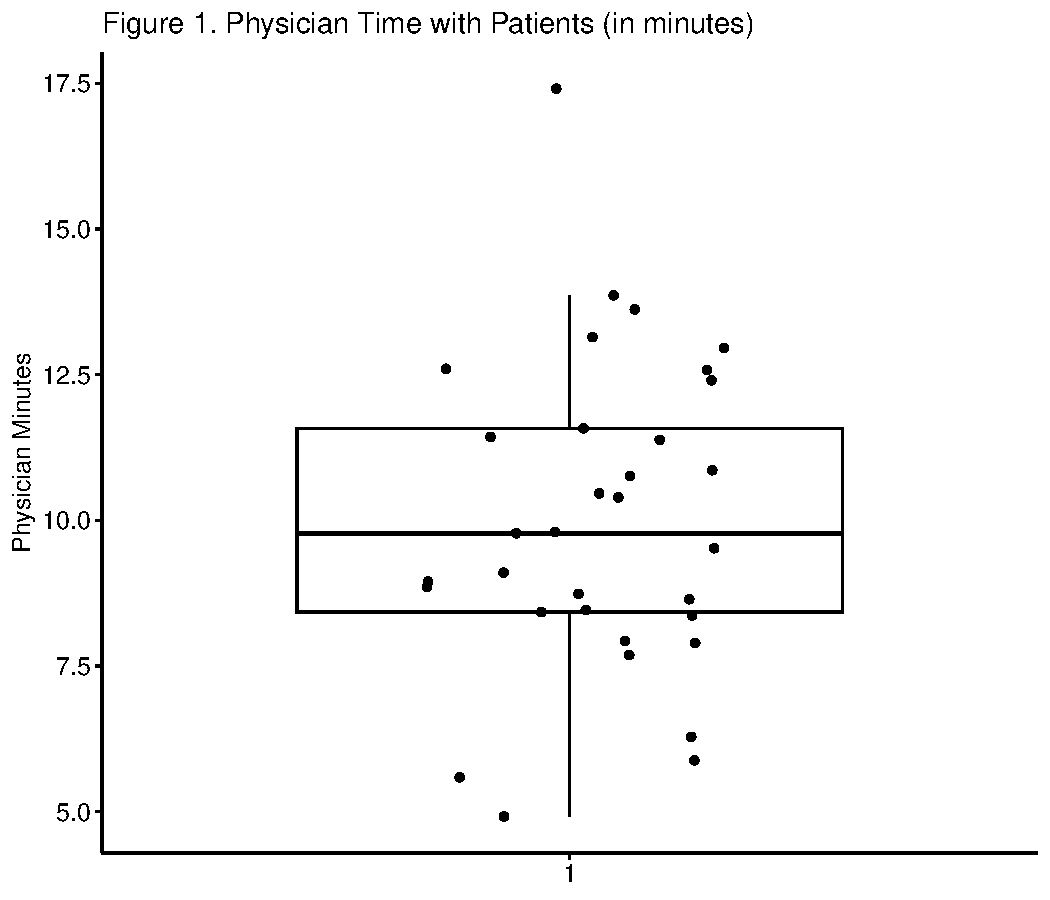
\includegraphics{04-tOneSample_files/figure-latex/unnamed-chunk-42-1.pdf}

Reflecting on these results, I must remind readers that this simulated data that is even further extrapolated. Although ``data'' informed both the amount of time spent by the physicians in the research study and data used as the test value, there are probably many reasons that the test value was not a good choice. For example, even though both contexts were ICU, palliative physicians may have a different standard of care than ICU physicians ``in general.''

\hypertarget{power-in-one-sample-t-tests}{%
\section{\texorpdfstring{Power in One-Sample \emph{t}-tests}{Power in One-Sample t-tests}}\label{power-in-one-sample-t-tests}}

Researchers often use power analysis packages to estimate the sample size needed to detect a statistically significant effect, if, in fact, there is one. Utilized another way, these tools allows us to determine the probability of detecting an effect of a given size with a given level of confidence. If the probability is unacceptably low, we may want to revise or stop. A helpful overview of power as well as guidelines for how to use the \emph{pwr} package can be found at a \href{https://www.statmethods.net/stats/power.html}{Quick-R website} \citep{kabacoff_power_2017}.

In Champely's \emph{pwr} package, we can conduct a power analysis for a variety of designs, including the one sample \emph{t}-test that we worked in this lesson. There are a number of interrelating elements of power:

\begin{itemize}
\tightlist
\item
  Sample size, \emph{n} refers to the number of observations; our vignette had 33
\item
  \emph{d} refers to the difference between means divided by the pooled standard deviation; ours was (10.01-1.23)/2.7; we can use the results from Cohen's \emph{d}.
\item
  \emph{power} refers to the power of a statistical test; conventionally it is set at .80
\item
  \emph{sig.level} refers to our desired alpha level; conventionally it is set at .05
\item
  \emph{type} indicates the type of test we ran; this was ``one.sample''
\item
  \emph{alternative} refers to whether the hypothesis is non-directional/two-tailed (``two.sided'') or directional/one-tailed(``less'' or ``greater'')
\end{itemize}

In this script, we must specify \emph{all-but-one} parameter; the remaining parameter must be defined as NULL. R will calculate the value for the missing parameter.

When we conduct a ``power analysis'' (i.e., the likelihood of a hypothesis test detecting an effect if there is one), we specify, ``power=NULL''. Using the data from our results, we learn from this first run, that our statistical power was 1.00. That is, given the value of the mean difference relative to the pooled standard deviation we had a 100\% chance of detecting a statistically significant effect if there was one.

\begin{Shaded}
\begin{Highlighting}[]
\NormalTok{pwr}\SpecialCharTok{::}\FunctionTok{pwr.t.test}\NormalTok{(}\AttributeTok{d =} \FloatTok{3.25}\NormalTok{, }\AttributeTok{n =} \DecValTok{33}\NormalTok{, }\AttributeTok{power =} \ConstantTok{NULL}\NormalTok{, }\AttributeTok{sig.level =} \FloatTok{0.05}\NormalTok{, }\AttributeTok{type =} \StringTok{"one.sample"}\NormalTok{,}
    \AttributeTok{alternative =} \StringTok{"two.sided"}\NormalTok{)}
\end{Highlighting}
\end{Shaded}

\begin{verbatim}

     One-sample t test power calculation 

              n = 33
              d = 3.25
      sig.level = 0.05
          power = 1
    alternative = two.sided
\end{verbatim}

Researchers frequently use these tools to estimate the sample size required to obtain a statistically significant effect. In these scenarios we set \emph{n} to \emph{NULL}.

\begin{Shaded}
\begin{Highlighting}[]
\NormalTok{pwr}\SpecialCharTok{::}\FunctionTok{pwr.t.test}\NormalTok{(}\AttributeTok{d =} \FloatTok{3.25}\NormalTok{, }\AttributeTok{n =} \ConstantTok{NULL}\NormalTok{, }\AttributeTok{power =} \FloatTok{0.8}\NormalTok{, }\AttributeTok{sig.level =} \FloatTok{0.05}\NormalTok{, }\AttributeTok{type =} \StringTok{"one.sample"}\NormalTok{,}
    \AttributeTok{alternative =} \StringTok{"two.sided"}\NormalTok{)}
\end{Highlighting}
\end{Shaded}

\begin{verbatim}

     One-sample t test power calculation 

              n = 3.006908
              d = 3.25
      sig.level = 0.05
          power = 0.8
    alternative = two.sided
\end{verbatim}

Shockingly, this suggests that a sample size of 3 could result in a statistically significant result. Let's see if this is true. Below I will re-simulate the data for the verbal scores, changing only the sample size:

\begin{Shaded}
\begin{Highlighting}[]
\FunctionTok{set.seed}\NormalTok{(}\DecValTok{220822}\NormalTok{)}
\NormalTok{rdfOneSample }\OtherTok{\textless{}{-}} \FunctionTok{data.frame}\NormalTok{(}\AttributeTok{rPhysMins =} \FunctionTok{rnorm}\NormalTok{(}\DecValTok{3}\NormalTok{, }\AttributeTok{mean =} \DecValTok{10}\NormalTok{, }\AttributeTok{sd =} \FloatTok{2.5}\NormalTok{))}

\FunctionTok{head}\NormalTok{(rdfOneSample)}
\end{Highlighting}
\end{Shaded}

\begin{verbatim}
  rPhysMins
1  9.097343
2 11.385558
3  8.424395
\end{verbatim}

With the newly simulated data, I will run the one-sample \emph{t}-test:

\begin{Shaded}
\begin{Highlighting}[]
\NormalTok{rstatix}\SpecialCharTok{::}\FunctionTok{t\_test}\NormalTok{(rdfOneSample, rPhysMins }\SpecialCharTok{\textasciitilde{}} \DecValTok{1}\NormalTok{, }\AttributeTok{mu =} \FloatTok{1.23}\NormalTok{, }\AttributeTok{detailed =} \ConstantTok{TRUE}\NormalTok{)}
\end{Highlighting}
\end{Shaded}

\begin{verbatim}
# A tibble: 1 x 12
  estimate .y.     group1 group2     n statistic      p    df conf.low conf.high
*    <dbl> <chr>   <chr>  <chr>  <int>     <dbl>  <dbl> <dbl>    <dbl>     <dbl>
1     9.64 rPhysM~ 1      null ~     3      9.38 0.0112     2     5.78      13.5
# i 2 more variables: method <chr>, alternative <chr>
\end{verbatim}

\begin{Shaded}
\begin{Highlighting}[]
\NormalTok{rstatix}\SpecialCharTok{::}\FunctionTok{cohens\_d}\NormalTok{(rdfOneSample, rPhysMins }\SpecialCharTok{\textasciitilde{}} \DecValTok{1}\NormalTok{, }\AttributeTok{ref.group =} \ConstantTok{NULL}\NormalTok{, }\AttributeTok{mu =} \FloatTok{1.23}\NormalTok{)}
\end{Highlighting}
\end{Shaded}

\begin{verbatim}
# A tibble: 1 x 6
  .y.       group1 group2     effsize     n magnitude
* <chr>     <chr>  <chr>        <dbl> <int> <ord>    
1 rPhysMins 1      null model    5.42     3 large    
\end{verbatim}

In this case our difference between the sample data and the external data is so huge, that a sample of three still nets a statistically significant result. This is unusual. Here's the \emph{t} string: \(t(2) = 9.379, p = 0.011, d = 5.415, CI95[5.78, 13.492]\).

\hypertarget{practice-problems-2}{%
\section{Practice Problems}\label{practice-problems-2}}

The suggestions for homework differ in degree of complexity. I encourage you to start with a problem that feels ``do-able'' and then try at least one more problem that challenges you in some way. Regardless, your choices should meet you where you are (e.g., in terms of your self-efficacy for statistics, your learning goals, and competing life demands). Using R packages, complete a one-sample \emph{t}-test.

Additionally, please complete at least one set of \emph{hand calculations}, that is using the code demonstrated in the chapter to work through the formulas that compute the one-sample \emph{t}-test. At this stage in your learning, you may ignore any missingness in your dataset by excluding all rows with missing data in your variables of interest.

\hypertarget{problem-1-rework-the-research-vignette-as-demonstrated-but-change-the-random-seed}{%
\subsection{Problem \#1: Rework the research vignette as demonstrated, but change the random seed}\label{problem-1-rework-the-research-vignette-as-demonstrated-but-change-the-random-seed}}

If this topic feels a bit overwhelming, simply change the random seed in the data simulation of the research vignette, then rework the problem. This should provide minor changes to the data but the results will likely be very similar. That said, don't be alarmed if what was non-significant in my working of the problem becomes significant. Our selection of \emph{p} \textless{} .05 (and the corresponding 95\% confidence interval) means that 5\% of the time there could be a difference in statistical significance.

\hypertarget{problem-2-rework-the-research-vignette-but-change-something-about-the-simulation}{%
\subsection{Problem \#2: Rework the research vignette, but change something about the simulation}\label{problem-2-rework-the-research-vignette-but-change-something-about-the-simulation}}

Rework the one sample \emph{t}-test in the lesson by changing something else about the simulation. Perhaps estimate another comparative number. The 1.23 was a dramatic difference from the mean of the research participants. Perhaps suggest (and, ideally, support with a reference) a different value. Alternatively, if you are interested in issues of power, specify a different sample size.

\hypertarget{problem-3-use-other-data-that-is-available-to-you}{%
\subsection{Problem \#3: Use other data that is available to you}\label{problem-3-use-other-data-that-is-available-to-you}}

Using data for which you have permission and access (e.g., IRB approved data you have collected or from your lab; data you simulate from a published article; data from an open science repository; data from other chapters in this OER), complete an independent samples \emph{t} test.

\hypertarget{grading-rubric}{%
\subsection{Grading Rubric}\label{grading-rubric}}

Regardless which option(s) you chose, use the elements in the grading rubric to guide you through the practice.

\begin{longtable}[]{@{}
  >{\raggedright\arraybackslash}p{(\columnwidth - 4\tabcolsep) * \real{0.5616}}
  >{\centering\arraybackslash}p{(\columnwidth - 4\tabcolsep) * \real{0.2466}}
  >{\centering\arraybackslash}p{(\columnwidth - 4\tabcolsep) * \real{0.1918}}@{}}
\toprule\noalign{}
\begin{minipage}[b]{\linewidth}\raggedright
Working the problem with R and R packages
\end{minipage} & \begin{minipage}[b]{\linewidth}\centering
Points Possible
\end{minipage} & \begin{minipage}[b]{\linewidth}\centering
Points Earned
\end{minipage} \\
\midrule\noalign{}
\endhead
\bottomrule\noalign{}
\endlastfoot
1. Narrate the research vignette, describing the variables and their role in the analysis & 5 & \_\_\_\_\_ \\
2. Simulate (or import) and format data & 5 & \_\_\_\_\_ \\
3. Evaluate statistical assumptions & 5 & \_\_\_\_\_ \\
4. Conduct a one sample \emph{t}-test (with an effect size) & 5 & \_\_\_\_\_ \\
5. APA style results with table(s) and figure & 5 & \_\_\_\_\_ \\
6. Conduct power analyses to determine the power of the current study and a recommended sample size & 5 & \_\_\_\_\_ \\
7. Explanation to grader & 5 & \_\_\_\_\_ \\
\textbf{Totals} & 35 & \_\_\_\_\_ \\
\end{longtable}

\begin{longtable}[]{@{}
  >{\raggedright\arraybackslash}p{(\columnwidth - 4\tabcolsep) * \real{0.5833}}
  >{\centering\arraybackslash}p{(\columnwidth - 4\tabcolsep) * \real{0.2083}}
  >{\raggedright\arraybackslash}p{(\columnwidth - 4\tabcolsep) * \real{0.2083}}@{}}
\toprule\noalign{}
\begin{minipage}[b]{\linewidth}\raggedright
Hand Calculations
\end{minipage} & \begin{minipage}[b]{\linewidth}\centering
Points Poss
\end{minipage} & \begin{minipage}[b]{\linewidth}\raggedright
Points Earned
\end{minipage} \\
\midrule\noalign{}
\endhead
\bottomrule\noalign{}
\endlastfoot
1. Using traditional NHST (null hypothesis testing language), state your null and alternative hypotheses & 2 & \\
2. Calculate the mean of your sample; identify the mean of your benchmarking sample & 2 & \\
3. Using the steps from the previous lesson, calculate the standard deviation of your sample. This should involve variables representing the mean, mean deviation, and mean deviation squared & 6 & \\
4. Calculate the one-sample \emph{t}-test & 4 & \\
5. Identify the degrees of freedom associated with your \emph{t}-test & 2 & \\
6. Locate the test critical value for your test & 2 & \\
7. Is the \emph{t}-test statistically significant? Why or why not? & 2 & \\
8. Calculate the confidence interval around your sample mean & 2 & \\
9. Calculate the effect size (i.e., Cohen's \emph{d} associated with your \emph{t}-test & 2 & \\
\textbf{Totals} & 24 & \\
\end{longtable}

\hypertarget{homeworked-example-2}{%
\section{Homeworked Example}\label{homeworked-example-2}}

\href{}{Screencast Link}

The one-sample test comes in handy when you want to compare your dataset to an external benchmark or standard. It can be a real helper in program evaluation

\emph{If you wanted to use this example and dataset as a basis for a homework assignment, you could select a different course (i.e., Multivariate or Psychometrics) and/or compare the mean for the ORG department (\(M = 4.1\)).}

\hypertarget{working-the-problem-with-r-and-r-packages-1}{%
\subsection{Working the Problem with R and R Packages}\label{working-the-problem-with-r-and-r-packages-1}}

\hypertarget{narrate-the-research-vignette-describing-the-variables-and-their-role-in-the-analysis}{%
\subsubsection{Narrate the research vignette, describing the variables and their role in the analysis}\label{narrate-the-research-vignette-describing-the-variables-and-their-role-in-the-analysis}}

From my course evaluation data, I want to ask the question, ``Are ratings for the Overall Instructor for the ANOVA course evals statistically significantly different from the overall departmental averages for that same item?'' In CPY the overall average for that specific item is 4.4.

\hypertarget{simulate-or-import-and-format-data}{%
\subsubsection{Simulate (or import) and format data}\label{simulate-or-import-and-format-data}}

The BIGdf is from a project that evaluated three changes to our own stats courses, over time. As a whole, this dataset violates a ton of assumptions of ANOVA, but we can create a tiny df and use it for demonstrations.

\begin{Shaded}
\begin{Highlighting}[]
\NormalTok{ReCdf }\OtherTok{\textless{}{-}} \FunctionTok{readRDS}\NormalTok{(}\StringTok{"ReC.rds"}\NormalTok{)}
\end{Highlighting}
\end{Shaded}

Let's first trim it to just students who took ANOVA

\begin{Shaded}
\begin{Highlighting}[]
\NormalTok{JustANOVA }\OtherTok{\textless{}{-}} \FunctionTok{subset}\NormalTok{(ReCdf, Course }\SpecialCharTok{==} \StringTok{"ANOVA"}\NormalTok{) }
\end{Highlighting}
\end{Shaded}

And further trim to our variable of interest

\begin{Shaded}
\begin{Highlighting}[]
\FunctionTok{library}\NormalTok{(tidyverse)}
\end{Highlighting}
\end{Shaded}

\begin{verbatim}
-- Attaching core tidyverse packages ------------------------ tidyverse 2.0.0 --
v dplyr     1.1.2     v readr     2.1.4
v forcats   1.0.0     v stringr   1.5.0
v ggplot2   3.4.2     v tibble    3.2.1
v lubridate 1.9.2     v tidyr     1.3.0
v purrr     1.0.1     
-- Conflicts ------------------------------------------ tidyverse_conflicts() --
x dplyr::filter() masks stats::filter()
x dplyr::lag()    masks stats::lag()
i Use the conflicted package (<http://conflicted.r-lib.org/>) to force all conflicts to become errors
\end{verbatim}

\begin{Shaded}
\begin{Highlighting}[]
\NormalTok{tiny1 }\OtherTok{\textless{}{-}}\NormalTok{ JustANOVA }\SpecialCharTok{\%\textgreater{}\%}
\NormalTok{    dplyr}\SpecialCharTok{::}\FunctionTok{select}\NormalTok{ (OvInstructor)}
\end{Highlighting}
\end{Shaded}

And further trim to non-missing data

\begin{Shaded}
\begin{Highlighting}[]
\NormalTok{tiny1 }\OtherTok{\textless{}{-}} \FunctionTok{na.omit}\NormalTok{(tiny1)}
\end{Highlighting}
\end{Shaded}

\begin{itemize}
\tightlist
\item
  Is the sample variable on a continuous scale of measurement and formatted as \emph{num} or \emph{int} in R?
\item
  Is the external score evaluated on the same continuous scale?
\end{itemize}

\begin{Shaded}
\begin{Highlighting}[]
\FunctionTok{str}\NormalTok{(tiny1}\SpecialCharTok{$}\NormalTok{OvInstructor)}
\end{Highlighting}
\end{Shaded}

\begin{verbatim}
 int [1:113] 5 4 4 3 5 3 5 4 3 5 ...
\end{verbatim}

Yes. The format for the OvInstructor variable is integer (which is numerical); the overall course evaluation is on an equivalent (1 to 5) scale.

\hypertarget{evaluate-statistical-assumptions}{%
\subsubsection{Evaluate statistical assumptions}\label{evaluate-statistical-assumptions}}

\begin{itemize}
\tightlist
\item
  Are the skew and kurtosis values within the range expected?
\item
  Does the distribution of the variable differ significantly from a normal distribution?
\end{itemize}

\begin{Shaded}
\begin{Highlighting}[]
\NormalTok{pastecs}\SpecialCharTok{::}\FunctionTok{stat.desc}\NormalTok{(tiny1}\SpecialCharTok{$}\NormalTok{OvInstructor, }\AttributeTok{norm=}\ConstantTok{TRUE}\NormalTok{)}
\end{Highlighting}
\end{Shaded}

\begin{verbatim}
               nbr.val               nbr.null                 nbr.na 
113.000000000000000000   0.000000000000000000   0.000000000000000000 
                   min                    max                  range 
  1.000000000000000000   5.000000000000000000   4.000000000000000000 
                   sum                 median                   mean 
473.000000000000000000   5.000000000000000000   4.185840707964601393 
               SE.mean           CI.mean.0.95                    var 
  0.095363991425895162   0.188951524765374329   1.027654867256637239 
               std.dev               coef.var               skewness 
  1.013733134141642456   0.242181488706142922  -0.984495621273390964 
              skew.2SE               kurtosis               kurt.2SE 
 -2.164227168444894378  -0.074100280830601939  -0.082121112321619227 
            normtest.W             normtest.p 
  0.772806906937811733   0.000000000006195409 
\end{verbatim}

The skew value is -9.84 and far exceeds the absolute value of 3. The skew.2SE is -2.164 (larger than the absolute value of 2.0) is consistent. Thus, we might have some concern about skew.

The kurtosis value is -7.410 and is below the absolute value of 10. The kurt.2SE value is -8.212 which is substantially larger than the absolute value of 2.0. Thus, we are similarly concerned about kurtosis.

The Shapiro wilk test value is 7.728 (\emph{p} \textless{} 0.001). This significant value suggests a distribution that is not normally distributed.

\hypertarget{conduct-a-one-sample-t-test-with-an-effect-size}{%
\subsubsection{\texorpdfstring{Conduct a one sample \emph{t} test (with an effect size)}{Conduct a one sample t test (with an effect size)}}\label{conduct-a-one-sample-t-test-with-an-effect-size}}

First, comparison to CPY

\begin{Shaded}
\begin{Highlighting}[]
\NormalTok{rstatix}\SpecialCharTok{::}\FunctionTok{t\_test}\NormalTok{(tiny1, OvInstructor }\SpecialCharTok{\textasciitilde{}} \DecValTok{1}\NormalTok{, }\AttributeTok{mu =} \FloatTok{4.4}\NormalTok{, }\AttributeTok{detailed =} \ConstantTok{TRUE}\NormalTok{)}
\end{Highlighting}
\end{Shaded}

\begin{verbatim}
# A tibble: 1 x 12
  estimate .y.     group1 group2     n statistic      p    df conf.low conf.high
*    <dbl> <chr>   <chr>  <chr>  <int>     <dbl>  <dbl> <dbl>    <dbl>     <dbl>
1     4.19 OvInst~ 1      null ~   113     -2.25 0.0267   112     4.00      4.37
# i 2 more variables: method <chr>, alternative <chr>
\end{verbatim}

We can begin to create our \emph{t} string:

\(t(112) = -2.246, p = 0.027, CI95(3.997, 4.374)\)

Let's interpret the results. With 112 degrees of freedom, our \emph{t} value is -2.245. Because the \emph{p} value is less than .05, this is statistically significant. This means that my course evaluations in ANOVA were statistically significantly lower than the average for CPY. We are 95\% confident that the true course evaluation mean (for my courses) fell between 3.997 and 4.374.

Let's calculate the effect size. we will use a Cohen's \emph{d} which is interpreted in standard deviation units.

\begin{Shaded}
\begin{Highlighting}[]
\NormalTok{rstatix}\SpecialCharTok{::}\FunctionTok{cohens\_d}\NormalTok{(tiny1, OvInstructor }\SpecialCharTok{\textasciitilde{}} \DecValTok{1}\NormalTok{, }\AttributeTok{ref.group =} \ConstantTok{NULL}\NormalTok{, }\AttributeTok{mu =} \FloatTok{4.4}\NormalTok{)}
\end{Highlighting}
\end{Shaded}

\begin{verbatim}
# A tibble: 1 x 6
  .y.          group1 group2     effsize     n magnitude
* <chr>        <chr>  <chr>        <dbl> <int> <ord>    
1 OvInstructor 1      null model  -0.211   113 small    
\end{verbatim}

Cohen's \emph{d} was 0.211. This is a small effect. We can add it to the \emph{t} string.

\(t(112) = -2.246, p = 0.027, CI95(3.997, 4.374), d = -0.211\)

\hypertarget{apa-style-results-with-tables-and-figure}{%
\subsubsection{APA style results with table(s) and figure}\label{apa-style-results-with-tables-and-figure}}

\begin{itemize}
\tightlist
\item
  t-test results should include t, df, p, d-or-eta, and CI95\%
\item
  Table
\item
  Figure
\item
  Grammar/style
\end{itemize}

\begin{quote}
A one-sample \emph{t}-test was used to evaluate whether the \emph{overall instructor} course evaluation ratings from the ANOVA courses were statistically significant from the departmental averages for the Clinical (CPY; \emph{M} = 4.4) department. The sample mean for the ANOVA course evaluations was 4.186 (\emph{SD} = 1.013).Although this mean was statistically significantly different from the average CPY course evaluation ratings of the same item, \(t(112) = -2.246, p = 0.027, CI95(3.997, 4.374)\), the effect size was quite small \((d = -0.211)\). A distribution of the ANOVA course ratings is found in Figure 1.
\end{quote}

\begin{Shaded}
\begin{Highlighting}[]
\NormalTok{ggpubr}\SpecialCharTok{::}\FunctionTok{ggboxplot}\NormalTok{(tiny1}\SpecialCharTok{$}\NormalTok{OvInstructor, }\AttributeTok{ylab =} \StringTok{"Course Evaluation Ratings"}\NormalTok{, }\AttributeTok{xlab =} \ConstantTok{FALSE}\NormalTok{,}
    \AttributeTok{add =} \StringTok{"jitter"}\NormalTok{, }\AttributeTok{title =} \StringTok{"Figure 1. Overall Instructor Ratings for ANOVA"}\NormalTok{)}
\end{Highlighting}
\end{Shaded}

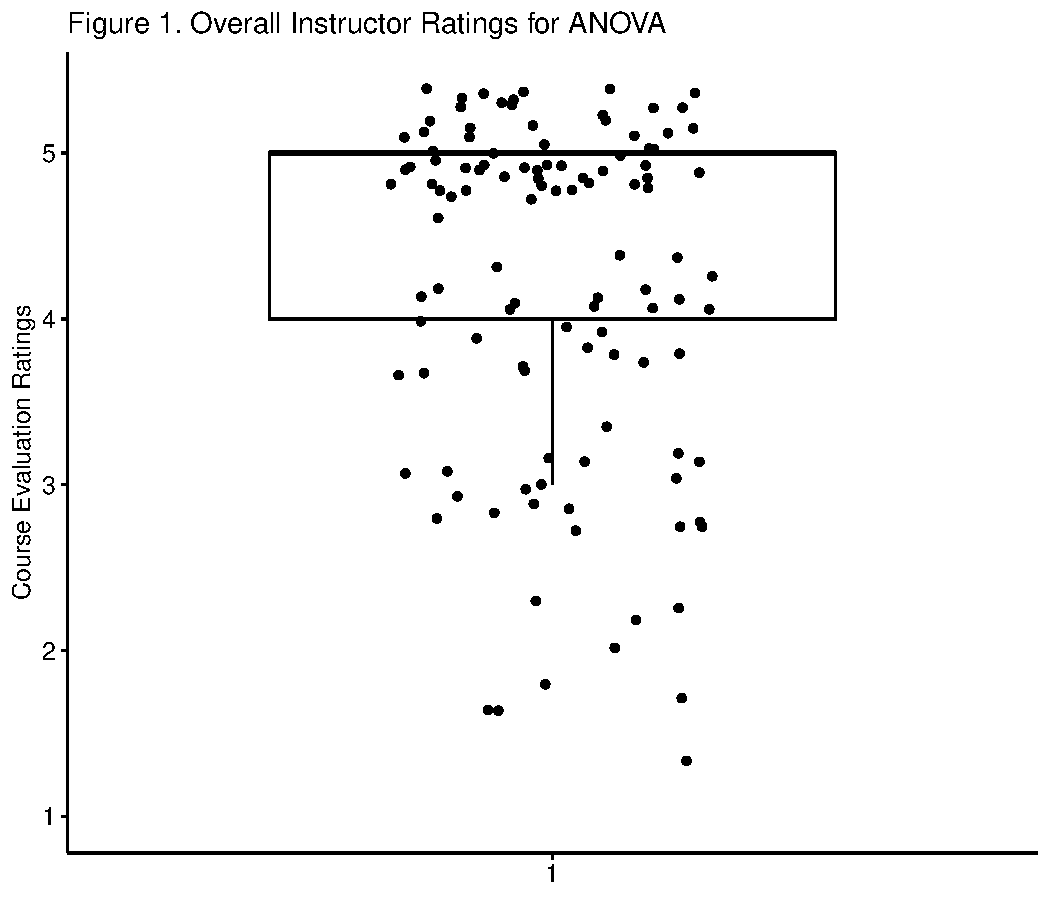
\includegraphics{04-tOneSample_files/figure-latex/unnamed-chunk-57-1.pdf}

\hypertarget{conduct-power-analyses-to-determine-the-power-of-the-current-study-and-a-recommended-sample-size}{%
\subsubsection{Conduct power analyses to determine the power of the current study and a recommended sample size}\label{conduct-power-analyses-to-determine-the-power-of-the-current-study-and-a-recommended-sample-size}}

A quick reminder that the \emph{d} in the power analysis is the difference between the means divided by the pooled standard deviation. This is the same as Cohen's d that we just calculated.

\begin{Shaded}
\begin{Highlighting}[]
\NormalTok{pwr}\SpecialCharTok{::}\FunctionTok{pwr.t.test}\NormalTok{(}\AttributeTok{d =} \SpecialCharTok{{-}}\FloatTok{0.211}\NormalTok{  , }\AttributeTok{n =} \DecValTok{113}\NormalTok{, }\AttributeTok{power =} \ConstantTok{NULL}\NormalTok{, }\AttributeTok{sig.level =} \FloatTok{0.05}\NormalTok{,}
    \AttributeTok{type =} \StringTok{"one.sample"}\NormalTok{, }\AttributeTok{alternative =} \StringTok{"two.sided"}\NormalTok{)}
\end{Highlighting}
\end{Shaded}

\begin{verbatim}

     One-sample t test power calculation 

              n = 113
              d = 0.211
      sig.level = 0.05
          power = 0.604022
    alternative = two.sided
\end{verbatim}

For the comparison to the CPY departmental average, power was 60\%. That is, given the value of the mean difference relative to the pooled standard deviation we had a 60\% chance of detecting a statistically significant effect if there was one.

\begin{Shaded}
\begin{Highlighting}[]
\NormalTok{pwr}\SpecialCharTok{::}\FunctionTok{pwr.t.test}\NormalTok{(}\AttributeTok{d =} \SpecialCharTok{{-}}\FloatTok{0.211}\NormalTok{, }\AttributeTok{n =} \ConstantTok{NULL}\NormalTok{, }\AttributeTok{power =} \FloatTok{0.8}\NormalTok{, }\AttributeTok{sig.level =} \FloatTok{0.05}\NormalTok{,}
    \AttributeTok{type =} \StringTok{"one.sample"}\NormalTok{, }\AttributeTok{alternative =} \StringTok{"two.sided"}\NormalTok{)}
\end{Highlighting}
\end{Shaded}

\begin{verbatim}

     One-sample t test power calculation 

              n = 178.226
              d = 0.211
      sig.level = 0.05
          power = 0.8
    alternative = two.sided
\end{verbatim}

For the CPY departmental comparison, the recommended sample size would be 178. This means there would need to be 178 individuals to find a statistically significant difference, if one existed.

\hypertarget{hand-calculations-1}{%
\subsection{Hand Calculations}\label{hand-calculations-1}}

\hypertarget{using-traditional-nhst-null-hypothesis-testing-language-state-your-null-and-alternative-hypotheses}{%
\subsubsection{Using traditional NHST (null hypothesis testing language), state your null and alternative hypotheses}\label{using-traditional-nhst-null-hypothesis-testing-language-state-your-null-and-alternative-hypotheses}}

\[
\begin{array}{ll}
H_0: & \mu = 4.4 \\
H_A: & \mu \neq 4.4
\end{array}
\]

\hypertarget{calculate-the-mean-of-your-sample-identify-the-mean-of-your-benchmarking-sample}{%
\subsubsection{Calculate the mean of your sample; identify the mean of your benchmarking sample}\label{calculate-the-mean-of-your-sample-identify-the-mean-of-your-benchmarking-sample}}

I will continue with the \emph{tiny1} dataset and calculate the mean of the OvInstructor variable from my ANOVA course evaluations.

\begin{Shaded}
\begin{Highlighting}[]
\FunctionTok{mean}\NormalTok{(tiny1}\SpecialCharTok{$}\NormalTok{OvInstructor, }\AttributeTok{na.rm=}\ConstantTok{TRUE}\NormalTok{)}
\end{Highlighting}
\end{Shaded}

\begin{verbatim}
[1] 4.185841
\end{verbatim}

The mean of my benchmarking sample is 4.4. This number is a ``departmental standard'' and did not need to be calculated by me for this purpose.

\hypertarget{using-the-steps-from-the-previous-lesson-hand-calculate-the-standard-deviation-of-your-sample.-this-should-involve-variables-representing-the-mean-mean-deviation-and-mean-deviation-squared}{%
\subsubsection{Using the steps from the previous lesson, hand-calculate the standard deviation of your sample. This should involve variables representing the mean, mean deviation, and mean deviation squared}\label{using-the-steps-from-the-previous-lesson-hand-calculate-the-standard-deviation-of-your-sample.-this-should-involve-variables-representing-the-mean-mean-deviation-and-mean-deviation-squared}}

\begin{Shaded}
\begin{Highlighting}[]
\CommentTok{\#first the mean}
\NormalTok{tiny1}\SpecialCharTok{$}\NormalTok{M\_OvInst }\OtherTok{\textless{}{-}} \FunctionTok{mean}\NormalTok{(tiny1}\SpecialCharTok{$}\NormalTok{OvInstructor, }\AttributeTok{na.rm=}\ConstantTok{TRUE}\NormalTok{)}
\CommentTok{\#second the mean deviation}
\NormalTok{tiny1}\SpecialCharTok{$}\NormalTok{Mdev\_OvInst }\OtherTok{\textless{}{-}}\NormalTok{ (tiny1}\SpecialCharTok{$}\NormalTok{OvInstructor}\SpecialCharTok{{-}}\NormalTok{tiny1}\SpecialCharTok{$}\NormalTok{M\_OvInst)}
\CommentTok{\#third the mean deviation squared}
\NormalTok{tiny1}\SpecialCharTok{$}\NormalTok{mdev2\_OvInst }\OtherTok{\textless{}{-}}\NormalTok{ (tiny1}\SpecialCharTok{$}\NormalTok{Mdev\_OvInst  }\SpecialCharTok{*}\NormalTok{ tiny1}\SpecialCharTok{$}\NormalTok{Mdev\_OvInst)}
\CommentTok{\#fourth the variance}
\NormalTok{var\_OvInst }\OtherTok{\textless{}{-}} \FunctionTok{sum}\NormalTok{(tiny1}\SpecialCharTok{$}\NormalTok{mdev2\_OvInst }\SpecialCharTok{/}\NormalTok{((}\FunctionTok{nrow}\NormalTok{(tiny1) }\SpecialCharTok{{-}} \DecValTok{1}\NormalTok{)))}
\NormalTok{var\_OvInst}
\end{Highlighting}
\end{Shaded}

\begin{verbatim}
[1] 1.027655
\end{verbatim}

\begin{Shaded}
\begin{Highlighting}[]
\CommentTok{\#finally the standard deviation}
\NormalTok{sd\_OvInst }\OtherTok{\textless{}{-}} \FunctionTok{sqrt}\NormalTok{(var\_OvInst)}
\NormalTok{sd\_OvInst}
\end{Highlighting}
\end{Shaded}

\begin{verbatim}
[1] 1.013733
\end{verbatim}

The variance is 1.028; the standard deviation is 1.014.

\begin{Shaded}
\begin{Highlighting}[]
\FunctionTok{sd}\NormalTok{(tiny1}\SpecialCharTok{$}\NormalTok{OvInstructor)}\CommentTok{\#checking my work}
\end{Highlighting}
\end{Shaded}

\begin{verbatim}
[1] 1.013733
\end{verbatim}

\hypertarget{calculate-the-one-sample-t-test}{%
\subsubsection{\texorpdfstring{Calculate the one-sample \emph{t}-test}{Calculate the one-sample t-test}}\label{calculate-the-one-sample-t-test}}

Here's the formula:

\[
t = \frac{\bar{X} - \mu}{\hat{\sigma}/\sqrt{N} }
\]

\begin{Shaded}
\begin{Highlighting}[]
\NormalTok{(}\FloatTok{4.185841} \SpecialCharTok{{-}} \FloatTok{4.4}\NormalTok{)}\SpecialCharTok{/}\NormalTok{(}\FloatTok{1.013733}\SpecialCharTok{/}\FunctionTok{sqrt}\NormalTok{(}\DecValTok{113}\NormalTok{))}
\end{Highlighting}
\end{Shaded}

\begin{verbatim}
[1] -2.245701
\end{verbatim}

\hypertarget{identify-the-degrees-of-freedom-associated-with-your-t-test}{%
\subsubsection{\texorpdfstring{Identify the degrees of freedom associated with your \emph{t}-test}{Identify the degrees of freedom associated with your t-test}}\label{identify-the-degrees-of-freedom-associated-with-your-t-test}}

For the one-sample \emph{t}-test, \(df = N - 1\). In our case

\begin{Shaded}
\begin{Highlighting}[]
\DecValTok{113} \SpecialCharTok{{-}} \DecValTok{1}
\end{Highlighting}
\end{Shaded}

\begin{verbatim}
[1] 112
\end{verbatim}

\hypertarget{locate-the-test-critical-value-for-your-test}{%
\subsubsection{Locate the test critical value for your test}\label{locate-the-test-critical-value-for-your-test}}

We can use a table of critical values for the one sample \emph{t}-test: \url{https://www.statology.org/t-distribution-table/}

A 2-tail test, when p - .05, with \textasciitilde120 individuals is 1.98

Or, this code:

\begin{Shaded}
\begin{Highlighting}[]
\FunctionTok{qt}\NormalTok{(}\AttributeTok{p =} \FloatTok{0.05}\SpecialCharTok{/}\DecValTok{2}\NormalTok{, }\AttributeTok{df =} \DecValTok{113}\NormalTok{, }\AttributeTok{lower.tail =} \ConstantTok{FALSE}\NormalTok{)}
\end{Highlighting}
\end{Shaded}

\begin{verbatim}
[1] 1.98118
\end{verbatim}

\hypertarget{is-the-t-test-statistically-significant-why-or-why-not}{%
\subsection{\texorpdfstring{Is the \emph{t}-test statistically significant? Why or why not?}{Is the t-test statistically significant? Why or why not?}}\label{is-the-t-test-statistically-significant-why-or-why-not}}

Yes \emph{t} = -2.245701 exceeds the (absolute) test critical value of 1.98.

\hypertarget{what-is-the-confidence-interval-around-your-sample-mean}{%
\subsubsection{What is the confidence interval around your sample mean?}\label{what-is-the-confidence-interval-around-your-sample-mean}}

Here is a reminder of the formula:

\[\bar{X} \pm t_{cv}(\frac{s}{\sqrt{n}})\]

\begin{Shaded}
\begin{Highlighting}[]
\NormalTok{(}\FloatTok{4.185841}\NormalTok{) }\SpecialCharTok{{-}}\NormalTok{ ((}\FloatTok{1.98118}\NormalTok{) }\SpecialCharTok{*}\NormalTok{ (}\FloatTok{1.013733}\SpecialCharTok{/}\FunctionTok{sqrt}\NormalTok{(}\DecValTok{113}\NormalTok{)))}
\end{Highlighting}
\end{Shaded}

\begin{verbatim}
[1] 3.996908
\end{verbatim}

\begin{Shaded}
\begin{Highlighting}[]
\NormalTok{(}\FloatTok{4.185841}\NormalTok{) }\SpecialCharTok{+}\NormalTok{ ((}\FloatTok{1.98118}\NormalTok{) }\SpecialCharTok{*}\NormalTok{ (}\FloatTok{1.013733}\SpecialCharTok{/}\FunctionTok{sqrt}\NormalTok{(}\DecValTok{113}\NormalTok{)))}
\end{Highlighting}
\end{Shaded}

\begin{verbatim}
[1] 4.374774
\end{verbatim}

We are 95\% confident that the sample mean for the student in the ANOVA classes is between 3.997, 4.375.

\hypertarget{calculate-the-effect-size-i.e.-cohens-d-associated-with-your-t-test}{%
\subsubsection{\texorpdfstring{Calculate the effect size (i.e., Cohen's \emph{d} associated with your \emph{t}-test}{Calculate the effect size (i.e., Cohen's d associated with your t-test}}\label{calculate-the-effect-size-i.e.-cohens-d-associated-with-your-t-test}}

A reminder of the two formula:

\[d = \frac{Mean Difference}{SD}=\frac{t}{\sqrt{N}}\]

\begin{Shaded}
\begin{Highlighting}[]
\CommentTok{\# First formula}
\NormalTok{(}\FloatTok{4.185841} \SpecialCharTok{{-}} \FloatTok{4.4}\NormalTok{)}\SpecialCharTok{/}\FloatTok{1.013733}
\end{Highlighting}
\end{Shaded}

\begin{verbatim}
[1] -0.2112578
\end{verbatim}

\begin{Shaded}
\begin{Highlighting}[]
\CommentTok{\# Second formula}
\SpecialCharTok{{-}}\FloatTok{2.245701}\SpecialCharTok{/}\FunctionTok{sqrt}\NormalTok{(}\DecValTok{113}\NormalTok{)}
\end{Highlighting}
\end{Shaded}

\begin{verbatim}
[1] -0.2112578
\end{verbatim}

\hypertarget{tIndSample}{%
\chapter{\texorpdfstring{Independent Samples \emph{t}-test}{Independent Samples t-test}}\label{tIndSample}}

\href{https://spu.hosted.panopto.com/Panopto/Pages/Viewer.aspx?pid=844ba297-e9ce-48cc-a49f-af01012b7900}{Screencasted Lecture Link}

\begin{Shaded}
\begin{Highlighting}[]
\FunctionTok{options}\NormalTok{(}\AttributeTok{scipen =} \DecValTok{999}\NormalTok{)  }\CommentTok{\#eliminates scientific notation}
\end{Highlighting}
\end{Shaded}

Researchers may wish to know if there are differences on a given outcome variable as a result of a dichotomous grouping variable. For example, during the COVID-19 pandemic, my research team asked if there were differences in the percentage of time that individuals wore facemasks as a result of 2020 Presidential voting trends (Republican or Democratic) of their county of residence. In these simple designs, the independent samples \emph{t}-test could be used to test the researchers' hypotheses.

\hypertarget{navigating-this-lesson-3}{%
\section{Navigating this Lesson}\label{navigating-this-lesson-3}}

There is just less than one hour of lecture. If you work through the materials with me, plan for an additional hour

While the majority of R objects and data you will need are created within the R script that sources the chapter, occasionally there are some that cannot be created from within the R framework. Additionally, sometimes links fail. All original materials are provided at the \href{https://github.com/lhbikos/ReCenterPsychStats}{Github site} that hosts the book. More detailed guidelines for ways to access all these materials are provided in the OER's \protect\hyperlink{ReCintro}{introduction}

\hypertarget{learning-objectives-3}{%
\subsection{Learning Objectives}\label{learning-objectives-3}}

Learning objectives from this lecture include the following:

\begin{itemize}
\tightlist
\item
  Recognize the research questions for which utilization of the independent samples \emph{t}-test would be appropriate.
\item
  Narrate the steps in conducting an independent samples \emph{t}-test, beginning with testing the statistical assumptions through writing up an APA style results section.
\item
  Calculate an independent samples \emph{t}-test in R (including effect sizes and 95\%CIs).
\item
  Interpret a 95\% confidence interval around a mean difference score.
\item
  Produce an APA style results section for an independent samples \emph{t}-test.
\item
  Determine a sample size that (given a set of parameters) would likely result in a statistically significant effect, if there was one.
\end{itemize}

\hypertarget{planning-for-practice-2}{%
\subsection{Planning for Practice}\label{planning-for-practice-2}}

The suggestions for homework vary in degree of complexity. The more complete descriptions at the end of the chapter follow these suggestions.

\begin{itemize}
\tightlist
\item
  Rework the independent samples \emph{t}-test in the lesson by changing the random seed in the code that simulates the data. This should provide minor changes to the data, but the results will likely be very similar.
\item
  Rework the independent samples \emph{t}-test in the lesson by changing something else about the simulation. For example, if you are interested in power, consider changing the sample size.
\item
  Use the simulated data that is provided, but use the nonverbal variable, instead.
\item
  Conduct an independent samples \emph{t}-test with data to which you have access and permission to use. This could include data you simulate on your own or from a published article.
\end{itemize}

\hypertarget{readings-resources-2}{%
\subsection{Readings \& Resources}\label{readings-resources-2}}

In preparing this chapter, I drew heavily from the following resource(s). Other resources are cited (when possible, linked) in the text with complete citations in the reference list.

\begin{itemize}
\tightlist
\item
  Navarro, D. (2020). Chapter 13: Comparing two means. In \href{https://learningstatisticswithr.com/}{Learning Statistics with R - A tutorial for Psychology Students and other Beginners}. Retrieved from \url{https://stats.libretexts.org/Bookshelves/Applied_Statistics/Book\%3A_Learning_Statistics_with_R_-_A_tutorial_for_Psychology_Students_and_other_Beginners_(Navarro)}

  \begin{itemize}
  \tightlist
  \item
    Navarro's OER includes a good mix of conceptual information about \emph{t}-tests as well as R code. My lesson integrates her approach as well as considering information from Field's \citeyearpar{field_discovering_2012} and Green and Salkind's \citep{green_using_2017} texts (as well as searching around on the internet).
  \end{itemize}
\item
  Elliott, A. M., Alexander, S. C., Mescher, C. A., Mohan, D., \& Barnato, A. E. (2016). Differences in Physicians' Verbal and Nonverbal Communication With Black and White Patients at the End of Life. \emph{Journal of Pain and Symptom Management, 51}(1), 1--8. \url{https://doi.org/10.1016/j.jpainsymman.2015.07.008}

  \begin{itemize}
  \tightlist
  \item
    The source of our research vignette.
  \end{itemize}
\end{itemize}

\hypertarget{packages-1}{%
\subsection{Packages}\label{packages-1}}

The script below will (a) check to see if the following packages are installed on your computer and, if not (b) install them.

\begin{Shaded}
\begin{Highlighting}[]
\CommentTok{\# will install the package if not already installed}
\CommentTok{\# if(!require(psych))\{install.packages(\textquotesingle{}psych\textquotesingle{})\}}
\CommentTok{\# if(!require(tidyverse))\{install.packages(\textquotesingle{}tidyverse\textquotesingle{})\}}
\CommentTok{\# if(!require(dplyr))\{install.packages(\textquotesingle{}dplyr\textquotesingle{})\}}
\CommentTok{\# if(!require(ggpubr))\{install.packages(\textquotesingle{}ggpubr\textquotesingle{})\}}
\CommentTok{\# if(!require(pwr))\{install.packages(\textquotesingle{}pwr\textquotesingle{})\}}
\CommentTok{\# if(!require(apaTables))\{install.packages(\textquotesingle{}apaTables\textquotesingle{})\}}
\CommentTok{\# if(!require(knitr))\{install.packages(\textquotesingle{}knitr\textquotesingle{})\}}
\CommentTok{\# if(!require(rstatix))\{install.packages(\textquotesingle{}rstatix\textquotesingle{})\}}
\end{Highlighting}
\end{Shaded}

\hypertarget{introducing-the-independent-samples-t-test}{%
\section{\texorpdfstring{Introducing the Independent Samples \emph{t}-Test}{Introducing the Independent Samples t-Test}}\label{introducing-the-independent-samples-t-test}}

The independent samples \emph{t}-test assesses whether the population mean of the test variable for one group differs from the population mean of the test variable for a second group. This \emph{t}-test can only accommodate two levels of a grouping variable (e.g., teachers/students, volunteers/employees, treatment/control) and the participants must be different in each group.

\begin{figure}
\centering

\includegraphics{images/ttests/conditions_paired.jpg}
\caption{An image of a row with two boxes labeled Condition A (in light blue) and Condition B (in dark blue). This represents the use of an independent samples \emph{t}-test to compare across conditions.}
\end{figure}

The comparison of two means is especially evident in the numerator of the formula. In the denominator we can see that the mean difference is adjusted by the standard error. At the outset, you should know that the formula in the denominator gets messy, but the formula, alone, provides an important conceptual map.

\[t = \frac{\bar{X}_1 - \bar{X}_2}{\mbox{SE}}\] If the researcher is interested in comparing the same participants' experiences across time or in different groups, they should consider using a \protect\hyperlink{tPaired}{paired samples \emph{t}-test}. Further, the independent samples \emph{t}-test is limited to a grouping variable with only two levels. If the researcher is interested in three or more levels, they should consider using a \protect\hyperlink{oneway}{one-way ANOVA}.

\hypertarget{workflow-for-independent-samples-t-test}{%
\subsection{\texorpdfstring{Workflow for Independent Samples \emph{t}-Test}{Workflow for Independent Samples t-Test}}\label{workflow-for-independent-samples-t-test}}

The following is a proposed workflow for conducting a independent samples \emph{t}-test.

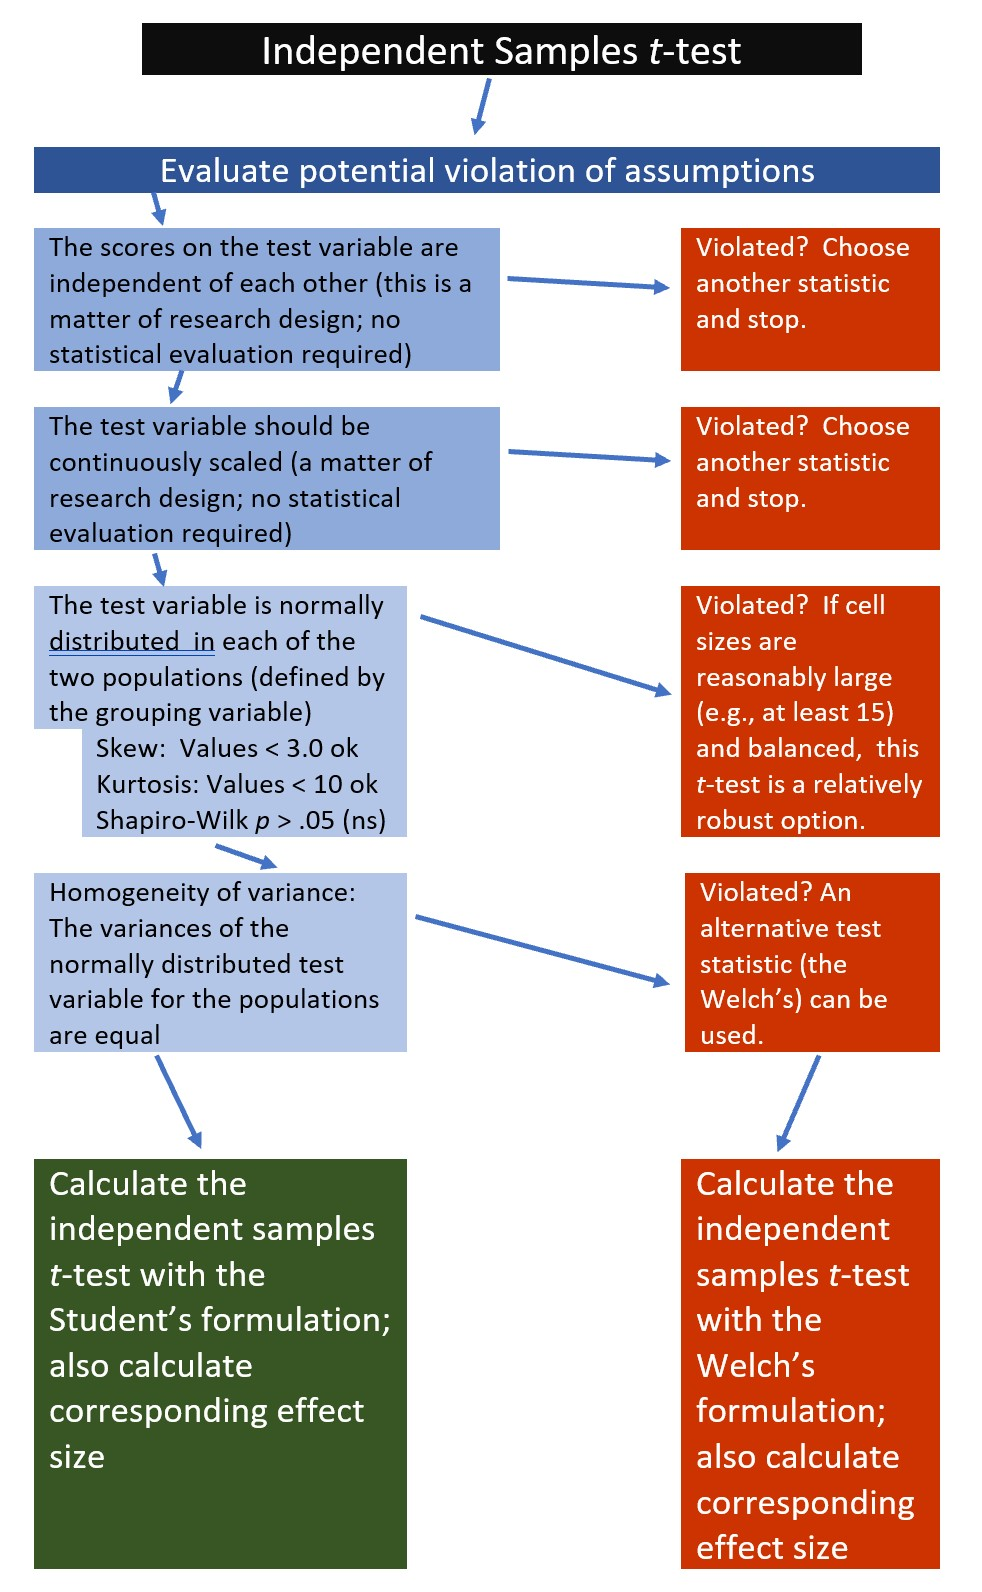
\includegraphics{images/ttests/IndSampleWrkFlw.jpg} If the data meets the assumptions associated with the research design (e.g., independence of observations and a continuously scaled metric), these are the steps for the analysis of an independent samples \emph{t}-test:

\begin{enumerate}
\def\labelenumi{\arabic{enumi}.}
\tightlist
\item
  Prepare (upload) data.
\item
  Explore data with

  \begin{itemize}
  \tightlist
  \item
    graphs
  \item
    descriptive statistics
  \end{itemize}
\item
  Assess normality via skew, kurtosis, and the Shapiro-Wilk test of normality
\item
  Consider the homogeneity of variance assumption and decide whether to use the Student's or Welch's formulation.
\item
  Compute the independent samples \emph{t}-test
\item
  Compute an effect size (frequently the \emph{d} or \emph{eta} statistic)
\item
  Manage Type I error
\item
  Sample size/power analysis (which you should think about first, but in the context of teaching statistics, it's more pedagogically sensible, here).
\end{enumerate}

\hypertarget{research-vignette-2}{%
\section{Research Vignette}\label{research-vignette-2}}

Empirically published articles where \emph{t}-tests are the primary statistic are difficult to locate. Having exhausted the psychology archives, I located this article in an interdisciplinary journal focused on palliative medicine. The research vignette for this lesson examined differences in physician's verbal and nonverbal communication with Black and White patients at the end of life \citep{elliott_differences_2016}.

Elliott and colleagues \citeyearpar{elliott_differences_2016} were curious to know if hospital-based physicians (56\% White, 26\% Asian, 7.4\% each Black and Hispanic) engaged in verbal and nonverbal communication differently with Black and White patients. Black and White patient participants were matched on characteristics deemed important to the researchers (e.g., critically and terminally ill, prognostically similar, expressed similar treatment preferences). Interactions in the intensive care unit were audio and video recorded and then coded on dimensions of verbal and nonverbal communication.

Because each physician saw a pair of patients (i.e., one Black patient and one White patient), the researchers utilized a paired samples, or dependent \emph{t}-test. This statistical choice was consistent with the element of the research design that controlled for physician effects through matching. Below are the primary findings of the study.

\begin{longtable}[]{@{}llll@{}}
\toprule\noalign{}
& Black Patients & White Patients & \\
\midrule\noalign{}
\endhead
\bottomrule\noalign{}
\endlastfoot
Category & \emph{Mean}(\emph{SD}) & \emph{Mean}(\emph{SD}) & \emph{p}-value \\
Verbal skill score (range 0 - 27) & 8.37(3.36) & 8.41(3.21) & 0.958 \\
Nonverbal skill score (range 0 - 5) & 2.68(.84) & 2.93(.77) & 0.014 \\
\end{longtable}

Although their design was more sophisticated (and, therefore, required the paired samples \emph{t}-test), Elliott et al. \citeyearpar{elliott_differences_2016} could have simply compared the outcome variables (e.g., verbal and nonverbal communication) as a function of their dichotomous variable, patient race (Black, White).

\hypertarget{data-simulation-1}{%
\subsection{Data Simulation}\label{data-simulation-1}}

In the data below, I have simulated the verbal and non-verbal communication variables using the means and standard deviations listed in the article. Further, I truncated them to fit within the assigned range. I created 33 sets each and assigned them to the Black or White level of the grouping variable.

\begin{Shaded}
\begin{Highlighting}[]
\FunctionTok{set.seed}\NormalTok{(}\DecValTok{220815}\NormalTok{)}
\CommentTok{\# sample size, M, and SD for Black then White patients}
\NormalTok{Verbal }\OtherTok{\textless{}{-}} \FunctionTok{c}\NormalTok{(}\FunctionTok{rnorm}\NormalTok{(}\DecValTok{33}\NormalTok{, }\AttributeTok{mean =} \FloatTok{8.37}\NormalTok{, }\AttributeTok{sd =} \FloatTok{3.36}\NormalTok{), }\FunctionTok{rnorm}\NormalTok{(}\DecValTok{33}\NormalTok{, }\AttributeTok{mean =} \FloatTok{8.41}\NormalTok{, }\AttributeTok{sd =} \FloatTok{3.21}\NormalTok{))}
\CommentTok{\# set upper bound}
\NormalTok{Verbal[Verbal }\SpecialCharTok{\textgreater{}} \DecValTok{27}\NormalTok{] }\OtherTok{\textless{}{-}} \DecValTok{27}
\CommentTok{\# set lower bound}
\NormalTok{Verbal[Verbal }\SpecialCharTok{\textless{}} \DecValTok{0}\NormalTok{] }\OtherTok{\textless{}{-}} \DecValTok{0}
\CommentTok{\# sample size, M, and SD for Black then White patients}
\NormalTok{Nonverbal }\OtherTok{\textless{}{-}} \FunctionTok{c}\NormalTok{(}\FunctionTok{rnorm}\NormalTok{(}\DecValTok{33}\NormalTok{, }\AttributeTok{mean =} \FloatTok{2.68}\NormalTok{, }\AttributeTok{sd =} \FloatTok{0.84}\NormalTok{), }\FunctionTok{rnorm}\NormalTok{(}\DecValTok{33}\NormalTok{, }\AttributeTok{mean =} \FloatTok{2.93}\NormalTok{,}
    \AttributeTok{sd =} \FloatTok{0.77}\NormalTok{))}
\CommentTok{\# set upper bound}
\NormalTok{Nonverbal[Nonverbal }\SpecialCharTok{\textgreater{}} \DecValTok{5}\NormalTok{] }\OtherTok{\textless{}{-}} \DecValTok{5}
\CommentTok{\# set lower bound}
\NormalTok{Nonverbal[Nonverbal }\SpecialCharTok{\textless{}} \DecValTok{0}\NormalTok{] }\OtherTok{\textless{}{-}} \DecValTok{0}

\NormalTok{ID }\OtherTok{\textless{}{-}} \FunctionTok{factor}\NormalTok{(}\FunctionTok{seq}\NormalTok{(}\DecValTok{1}\NormalTok{, }\DecValTok{66}\NormalTok{))}
\CommentTok{\# name factors and identify how many in each group; should be in same}
\CommentTok{\# order as first row of script}
\NormalTok{PatientRace }\OtherTok{\textless{}{-}} \FunctionTok{c}\NormalTok{(}\FunctionTok{rep}\NormalTok{(}\StringTok{"Black"}\NormalTok{, }\DecValTok{33}\NormalTok{), }\FunctionTok{rep}\NormalTok{(}\StringTok{"White"}\NormalTok{, }\DecValTok{33}\NormalTok{))}
\CommentTok{\# groups the 3 variables into a single df: ID\#, DV, condition}
\NormalTok{dfIndSamples }\OtherTok{\textless{}{-}} \FunctionTok{data.frame}\NormalTok{(ID, PatientRace, Verbal, Nonverbal)}
\end{Highlighting}
\end{Shaded}

With our data in hand, let's inspect its structure (i.e., the measurement scales for the variables) to see if they are appropriate.

\begin{Shaded}
\begin{Highlighting}[]
\FunctionTok{str}\NormalTok{(dfIndSamples)}
\end{Highlighting}
\end{Shaded}

\begin{verbatim}
'data.frame':   66 obs. of  4 variables:
 $ ID         : Factor w/ 66 levels "1","2","3","4",..: 1 2 3 4 5 6 7 8 9 10 ...
 $ PatientRace: chr  "Black" "Black" "Black" "Black" ...
 $ Verbal     : num  2.76 5.73 6.81 8.68 9.1 ...
 $ Nonverbal  : num  3.41 4.02 1.62 2.52 2.11 ...
\end{verbatim}

The verbal and nonverbal variables are quasi-interval scale variables. Therefore, the numerical scale is correctly assigned by R. In contrast, patient race is a nominal variable and should be a factor. In their article, Elliot et al. \citeyearpar{elliott_differences_2016} assigned Black as the baseline variable and White as the comparison variable. Because R orders factors alphabetically, and ``Black'' precedes ``White'', this would happen automatically. Because creating ordered factors is a useful skill, I will write out the full code.

\begin{Shaded}
\begin{Highlighting}[]
\NormalTok{dfIndSamples}\SpecialCharTok{$}\NormalTok{PatientRace }\OtherTok{\textless{}{-}} \FunctionTok{factor}\NormalTok{(dfIndSamples}\SpecialCharTok{$}\NormalTok{PatientRace, }\AttributeTok{levels =} \FunctionTok{c}\NormalTok{(}\StringTok{"Black"}\NormalTok{,}
    \StringTok{"White"}\NormalTok{))}
\end{Highlighting}
\end{Shaded}

Let's again check the formatting of the variables:

\begin{Shaded}
\begin{Highlighting}[]
\FunctionTok{str}\NormalTok{(dfIndSamples)}
\end{Highlighting}
\end{Shaded}

\begin{verbatim}
'data.frame':   66 obs. of  4 variables:
 $ ID         : Factor w/ 66 levels "1","2","3","4",..: 1 2 3 4 5 6 7 8 9 10 ...
 $ PatientRace: Factor w/ 2 levels "Black","White": 1 1 1 1 1 1 1 1 1 1 ...
 $ Verbal     : num  2.76 5.73 6.81 8.68 9.1 ...
 $ Nonverbal  : num  3.41 4.02 1.62 2.52 2.11 ...
\end{verbatim}

The four variables of interest are now correctly formatted as \emph{num} and \emph{factor}.

Below is code for saving (and then importing) the data in .csv or .rds files. I make choices about saving data based on what I wish to do with the data. If I want to manipulate the data outside of R, I will save it as a .csv file. It is easy to open .csv files in Excel. A limitation of the .csv format is that it does not save any restructuring or reformatting of variables. For this lesson, this is not an issue.

Here is code for saving the data as a .csv and then reading it back into R. I have hashtagged these out, so you will need to remove the hashtags if you wish to run any of these operations. If you have simulated the data (above), you do not need to save and then re-import the data.

\begin{Shaded}
\begin{Highlighting}[]
\CommentTok{\# writing the simulated data as a .csv write.table(dfIndSamples, file}
\CommentTok{\# = \textquotesingle{}dfIndSamples.csv\textquotesingle{}, sep = \textquotesingle{},\textquotesingle{}, col.names=TRUE, row.names=FALSE)}
\CommentTok{\# at this point you could clear your environment and then bring the}
\CommentTok{\# data back in as a .csv reading the data back in as a .csv file}
\CommentTok{\# dfIndSamples\textless{}{-} read.csv (\textquotesingle{}dfIndSamples.csv\textquotesingle{}, header = TRUE)}
\end{Highlighting}
\end{Shaded}

The .rds form of saving variables preserves any formatting (e.g., creating ordered factors) of the data. A limitation is that these files are not easily opened in Excel. Here is the hashtagged code (remove hashtags if you wish to do this) for writing (and then reading) this data as an .rds file.

\begin{Shaded}
\begin{Highlighting}[]
\CommentTok{\# saveRDS(dfIndSamples, \textquotesingle{}dfIndSamples.rds\textquotesingle{}) dfIndSamples \textless{}{-}}
\CommentTok{\# readRDS(\textquotesingle{}dfIndSamples.rds\textquotesingle{}) str(dfIndSamples)}
\end{Highlighting}
\end{Shaded}

\hypertarget{quick-peek-at-the-data-1}{%
\subsection{Quick Peek at the Data}\label{quick-peek-at-the-data-1}}

Plotting the data is a helpful early step in any data analysis. Further, visualizing the data can help us with a conceptual notion of the statistic we are utilizing. The \emph{ggpubr} package is one of my go-to-tools for quick and easy plots of data. Boxplots are terrific for data that is grouped. A helpful \href{https://rpkgs.datanovia.com/ggpubr/}{tutorial} for boxplots (and related plots) can be found at datanovia.

In the code below I introduced the colors by identifying the grouping variable and assigning colors. Those color codes are the ``Hex'' codes you find in the custom color palette in your word processing program.

I am also fond of plotting each case with the command, \emph{add = ``jitter''}. To increase your comfort and confidence in creating figures (and with other tools) try deleting and adding back in different commands. This is how to distinguish between the essential and the elective elements of the code.

\begin{Shaded}
\begin{Highlighting}[]
\NormalTok{ggpubr}\SpecialCharTok{::}\FunctionTok{ggboxplot}\NormalTok{(dfIndSamples, }\AttributeTok{x =} \StringTok{"PatientRace"}\NormalTok{, }\AttributeTok{y =} \StringTok{"Verbal"}\NormalTok{, }\AttributeTok{color =} \StringTok{"PatientRace"}\NormalTok{,}
    \AttributeTok{palette =} \FunctionTok{c}\NormalTok{(}\StringTok{"\#00AFBB"}\NormalTok{, }\StringTok{"\#FC4E07"}\NormalTok{), }\AttributeTok{add =} \StringTok{"jitter"}\NormalTok{)}
\end{Highlighting}
\end{Shaded}

\includegraphics{05-tIndSample_files/figure-latex/unnamed-chunk-10-1.pdf} The box of the boxplot covers the middle 50\% (the interquartile range). The horizontal line is the median. The whiskers represent three standard deviations above and below the mean. Any dots are outliers.

\hypertarget{working-the-independent-samples-t-test-by-hand}{%
\section{\texorpdfstring{Working the Independent Samples \emph{t}-Test (by hand)}{Working the Independent Samples t-Test (by hand)}}\label{working-the-independent-samples-t-test-by-hand}}

\hypertarget{stating-the-hypothesis-1}{%
\subsection{Stating the Hypothesis}\label{stating-the-hypothesis-1}}

In this lesson, I will focus on differences in the verbal communication variable. Specifically, I hypothesize that physician verbal communication scores for Black and White patients will differ. In the hypotheses below, the null hypothesis (\(H_0\)) states that the two means are equal; the alternative hypothesis (\(H_A\)) states that the two means are not equal.

\[
\begin{array}{ll}
H_0: & \mu_1 = \mu_2  \\
H_A: & \mu_1 \neq \mu_2
\end{array}
\]

\hypertarget{calculating-the-t-test-1}{%
\subsection{\texorpdfstring{Calculating the \emph{t}-Test}{Calculating the t-Test}}\label{calculating-the-t-test-1}}

Earlier I presented a formula for the independent samples \emph{t}-test.

\[t = \frac{\bar{X}_1 - \bar{X}_2}{\mbox{SE}}\] There are actually two formulations of the \emph{t}-test. Student's version can be used when there is no violation of the homogeneity of variance assumption; Welch's can be used when the homogeneity of variance assumption is violated. For the hand-calculation demonstration, I will only demonstrate the formula in the most ideal of circumstances, that is: there is no violation of the homogeneity of variance assumption and sample sizes are equal.

Even so, while the formula seems straightforward enough, calculating the SE in the denominator gets a little spicy:

\[t = \frac{\bar{X_{1}} -\bar{X_{2}}}{\sqrt{\frac{s_{1}^{2}}{N_{1}}+\frac{s_{2}^{2}}{N_{2}}}}\] Let's first calculate the SE -- the value of the denominator. For this, we need the standard deviations for the dependent variable (verbal) for both levels of patient race. We obtained these earlier when we used the \emph{describeBy()} function in the \emph{psych} package.

The standard deviation of the verbal variable for the levels in the patient race group were 2.99 for Black patients and 3.20 for White patients; the \emph{N} in both our groups is 33. We can do the denominator math right in an R chunk:

\begin{Shaded}
\begin{Highlighting}[]
\FunctionTok{sqrt}\NormalTok{((}\FloatTok{2.985}\SpecialCharTok{\^{}}\DecValTok{2}\SpecialCharTok{/}\DecValTok{33}\NormalTok{) }\SpecialCharTok{+}\NormalTok{ (}\FloatTok{3.203}\SpecialCharTok{\^{}}\DecValTok{2}\SpecialCharTok{/}\DecValTok{33}\NormalTok{))}
\end{Highlighting}
\end{Shaded}

\begin{verbatim}
[1] 0.7621627
\end{verbatim}

Our \emph{SE} = 0.762

With the simplification of the denominator, we can easily calculate the independent sample \emph{t}-test.

\[t = \frac{\bar{X_{1}} -\bar{X_{2}}}{SE}\]

\begin{Shaded}
\begin{Highlighting}[]
\NormalTok{(}\FloatTok{7.615} \SpecialCharTok{{-}} \FloatTok{8.891}\NormalTok{)}\SpecialCharTok{/}\FloatTok{0.762}
\end{Highlighting}
\end{Shaded}

\begin{verbatim}
[1] -1.674541
\end{verbatim}

Hopefully, this hand-calculation provided an indication of how the means, standard deviation, and sample sizes contribute to the estimate of this \emph{t}-test value. Now we ask, ``But it is statistically significant?''

\hypertarget{statistical-significance-1}{%
\subsubsection{Statistical Significance}\label{statistical-significance-1}}

The question of statistical significance testing invokes NHST (null hypothesis significance testing). In the case of the independent samples \emph{t}-test, the null hypothesis is that the two means are equal; the alternative is that they are not equal. Our test is of the null hypothesis. When the probability (\emph{p}) is less than the value we specify (usually .05), we are 95\% certain that the two means are not equal. Thus, we reject the null hypothesis (the one we tested) in favor of the alternative (that the means are not equal).

\[
\begin{array}{ll}
H_0: & \mu_1 = \mu_2  \\
H_A: & \mu_1 \neq \mu_2
\end{array}
\] Although still used, NHST has its critiques. Among the critiques are the layers of logic and confusing language as we interpret the results.

Our \emph{t}-value was -1.675. We compare this value to the test critical value in a table of \emph{t} critical values. In-so-doing we must know our degrees of freedom. In the test that involves two levels of a grouping value, we will use \(N -1\) as the value for degrees of freedom. We must also specify the \emph{p} value (in our case .05) and whether-or-not our hypothesis is unidirectional or bi-directional. Our question only asked, ``Are the verbal communication levels different?'' In this case, the test is two-tailed, or bi-directional.

Let's return to the \href{https://www.statology.org/t-distribution-table/}{table of critical values} for the \emph{t} distribution to compare our \emph{t}-value (-1.675) to the column that is appropriate for our:

\begin{itemize}
\tightlist
\item
  Degrees of freedom (in this case \(N-2\) or 64)

  \begin{itemize}
  \tightlist
  \item
    We have two levels of a grouping value; for each our df is \(N-1\)
  \end{itemize}
\item
  Alpha, as represented by \(p < .05\)
\item
  Specification as a one-tailed or two-tailed test

  \begin{itemize}
  \tightlist
  \item
    Our alternative hypothesis made no prediction about the direction of the difference; therefore we will use a two-tailed test
  \end{itemize}
\end{itemize}

In the above linked table of critical values, when the degrees of freedom reaches 30, there larger intervals. We will use the row representing degrees of freedom of 60. If our \emph{t}-test value is lower than an absolute value of -2 or greater than the absolute value of 2, then our means are statistically significantly different from each other. In our case, we have not achieved statistical significance and we cannot say that the means are different. The \emph{t} string would look like this: \(t(64) = -1.675, p > .05\)

We can also use the \emph{qt()} function in base R. In the script below, I have indicated an alpha of .05. The ``2'' that follows indicates I want a two-tailed test. The 64 represents my degrees of freedom (\(N-2\)). In a two-tailed test, the regions of rejection will be below the lowerbound (lower.tail=TRUE) and above the upperbound (lower.tail=FALSE).

\begin{Shaded}
\begin{Highlighting}[]
\FunctionTok{qt}\NormalTok{(}\FloatTok{0.05}\SpecialCharTok{/}\DecValTok{2}\NormalTok{, }\DecValTok{64}\NormalTok{, }\AttributeTok{lower.tail =} \ConstantTok{TRUE}\NormalTok{)}
\end{Highlighting}
\end{Shaded}

\begin{verbatim}
[1] -1.99773
\end{verbatim}

\begin{Shaded}
\begin{Highlighting}[]
\FunctionTok{qt}\NormalTok{(}\FloatTok{0.05}\SpecialCharTok{/}\DecValTok{2}\NormalTok{, }\DecValTok{64}\NormalTok{, }\AttributeTok{lower.tail =} \ConstantTok{FALSE}\NormalTok{)}
\end{Highlighting}
\end{Shaded}

\begin{verbatim}
[1] 1.99773
\end{verbatim}

Given the large intervals, it makes sense that this test critical value is slightly different than the one from the table.

\hypertarget{confidence-intervals-1}{%
\subsubsection{Confidence Intervals}\label{confidence-intervals-1}}

How confident are we in our result? With independent samples \emph{t}-tests, it is common to report an interval in which we are 95\% confident that our true mean difference exists. Below is the formula, which involves:

\begin{itemize}
\tightlist
\item
  \(\bar{X_{1}}-\bar{X_{2}}\) the difference in the means
\item
  \(t_{cv}\) the test critical value for a two-tailed model (even if the hypothesis was one-tailed) where \(\alpha = .05\) and the degrees of freedom are \(N-2\)
\item
  \(SE\) the standard error used in the denominator of the test statistic
\end{itemize}

\[(\bar{X_{1}} -\bar{X_{2})} \pm  t_{cv}(SE)\] Let's calculate it:

First, let's get the proper \emph{t} critical value. Even though these are identical to the one above, I am including them again. Why? Because if the original hypothesis had been one-tailed, we would need to calculate a two-tailed confidence interval; this is a placeholder to remind us.

\begin{Shaded}
\begin{Highlighting}[]
\FunctionTok{qt}\NormalTok{(}\FloatTok{0.05}\SpecialCharTok{/}\DecValTok{2}\NormalTok{, }\DecValTok{64}\NormalTok{, }\AttributeTok{lower.tail =} \ConstantTok{TRUE}\NormalTok{)}
\end{Highlighting}
\end{Shaded}

\begin{verbatim}
[1] -1.99773
\end{verbatim}

\begin{Shaded}
\begin{Highlighting}[]
\FunctionTok{qt}\NormalTok{(}\FloatTok{0.05}\SpecialCharTok{/}\DecValTok{2}\NormalTok{, }\DecValTok{64}\NormalTok{, }\AttributeTok{lower.tail =} \ConstantTok{FALSE}\NormalTok{)}
\end{Highlighting}
\end{Shaded}

\begin{verbatim}
[1] 1.99773
\end{verbatim}

With this in hand, let's calculate the confidence intervals.

\begin{Shaded}
\begin{Highlighting}[]
\NormalTok{(}\FloatTok{7.614} \SpecialCharTok{{-}} \FloatTok{8.891}\NormalTok{) }\SpecialCharTok{{-}}\NormalTok{ (}\FloatTok{1.99773} \SpecialCharTok{*} \FloatTok{0.762}\NormalTok{)}
\end{Highlighting}
\end{Shaded}

\begin{verbatim}
[1] -2.79927
\end{verbatim}

\begin{Shaded}
\begin{Highlighting}[]
\NormalTok{(}\FloatTok{7.614} \SpecialCharTok{{-}} \FloatTok{8.891}\NormalTok{) }\SpecialCharTok{+}\NormalTok{ (}\FloatTok{1.99773} \SpecialCharTok{*} \FloatTok{0.762}\NormalTok{)}
\end{Highlighting}
\end{Shaded}

\begin{verbatim}
[1] 0.2452703
\end{verbatim}

These values indicate the range of scores in which we are 95\% confident that our true mean difference (\(\bar{X_{1}}-\bar{X_{2}}\)) lies. Stated another way, we are 95\% confident that the true mean difference lies between -2.80 and 0.25 Because this interval crosses zero, we cannot rule out that the true mean difference is 0.00. This result is consistent with our non-significant \emph{p} value. For these types of statistics, the 95\% confidence interval and \emph{p} value will always be yoked together.

\hypertarget{effect-size-1}{%
\subsubsection{Effect Size}\label{effect-size-1}}

Whereas \emph{p} values address statistical significance, effect sizes address the magnitude of difference. There are two common effect sizes that are used with the independent samples \emph{t}-test. The first is the \emph{d} statistic, which measures, in standard deviation units, the distance between the two means. The simplest formula involves the \emph{t} value and sample sizes:

\[d = t\sqrt{\frac{N_{1}+N_{2}}{N_{1}N_{2}}}\]

With a \emph{t} value of -1.675 and sample sizes at 33 each, we can easily calculate this. Small, medium, and large sizes for the \emph{d} statistic are .2, .5, and .8, respectively (irrespective of sign).

\begin{Shaded}
\begin{Highlighting}[]
\SpecialCharTok{{-}}\FloatTok{1.675} \SpecialCharTok{*}\NormalTok{ (}\FunctionTok{sqrt}\NormalTok{((}\DecValTok{33} \SpecialCharTok{+} \DecValTok{33}\NormalTok{)}\SpecialCharTok{/}\NormalTok{(}\DecValTok{33} \SpecialCharTok{*} \DecValTok{33}\NormalTok{)))}
\end{Highlighting}
\end{Shaded}

\begin{verbatim}
[1] -0.4123565
\end{verbatim}

Our value, -0.412 suggests a small-to-medium effect size. We might wonder why it wasn't statistically significant? Later we will discuss power and the relationship between sample size, one vs.~two-tailed hypotheses, and effect sizes.

Eta square, \(\eta^2\) is the proportion of variance of a test variable that is a function of the grouping variable. A value of 0 indicates that the difference in the mean scores is equal to 0, where a value of 1 indicates that the sample means differ, and the test scores do not differ within each group. The following equation can be used to compute \(\eta^2\). Conventionally, values of .01, .06, and .14 are considered to be small, medium, and large effect sizes, respectively.

\[\eta^{2} =\frac{t^{2}}{t^{2}+(N_{1}+N_{2}-2)}\] Let's calculate it:

\begin{Shaded}
\begin{Highlighting}[]
\NormalTok{(}\SpecialCharTok{{-}}\FloatTok{1.6745} \SpecialCharTok{*} \SpecialCharTok{{-}}\FloatTok{1.6745}\NormalTok{)}\SpecialCharTok{/}\NormalTok{((}\SpecialCharTok{{-}}\FloatTok{1.6745} \SpecialCharTok{*} \SpecialCharTok{{-}}\FloatTok{1.6745}\NormalTok{) }\SpecialCharTok{+}\NormalTok{ (}\DecValTok{33} \SpecialCharTok{+} \DecValTok{33} \SpecialCharTok{{-}} \DecValTok{2}\NormalTok{))}
\end{Highlighting}
\end{Shaded}

\begin{verbatim}
[1] 0.04197282
\end{verbatim}

Similarly, the \(\eta^2\) is small-to-medium.

\hypertarget{working-the-independent-samples-t-test-with-r-packages}{%
\section{\texorpdfstring{Working the Independent Samples \emph{t}-Test with R Packages}{Working the Independent Samples t-Test with R Packages}}\label{working-the-independent-samples-t-test-with-r-packages}}

Let's rework the problem in R. We start at the top of the flowchart, evaluating the statistical assumptions.

\hypertarget{evaluating-the-statistical-assumptions-1}{%
\subsection{Evaluating the Statistical Assumptions}\label{evaluating-the-statistical-assumptions-1}}

With an eye on our data, we can begin to explore the statistical assumptions associated with the independent samples \emph{t}-test. Here's where we are in the workflow:

\begin{figure}
\centering
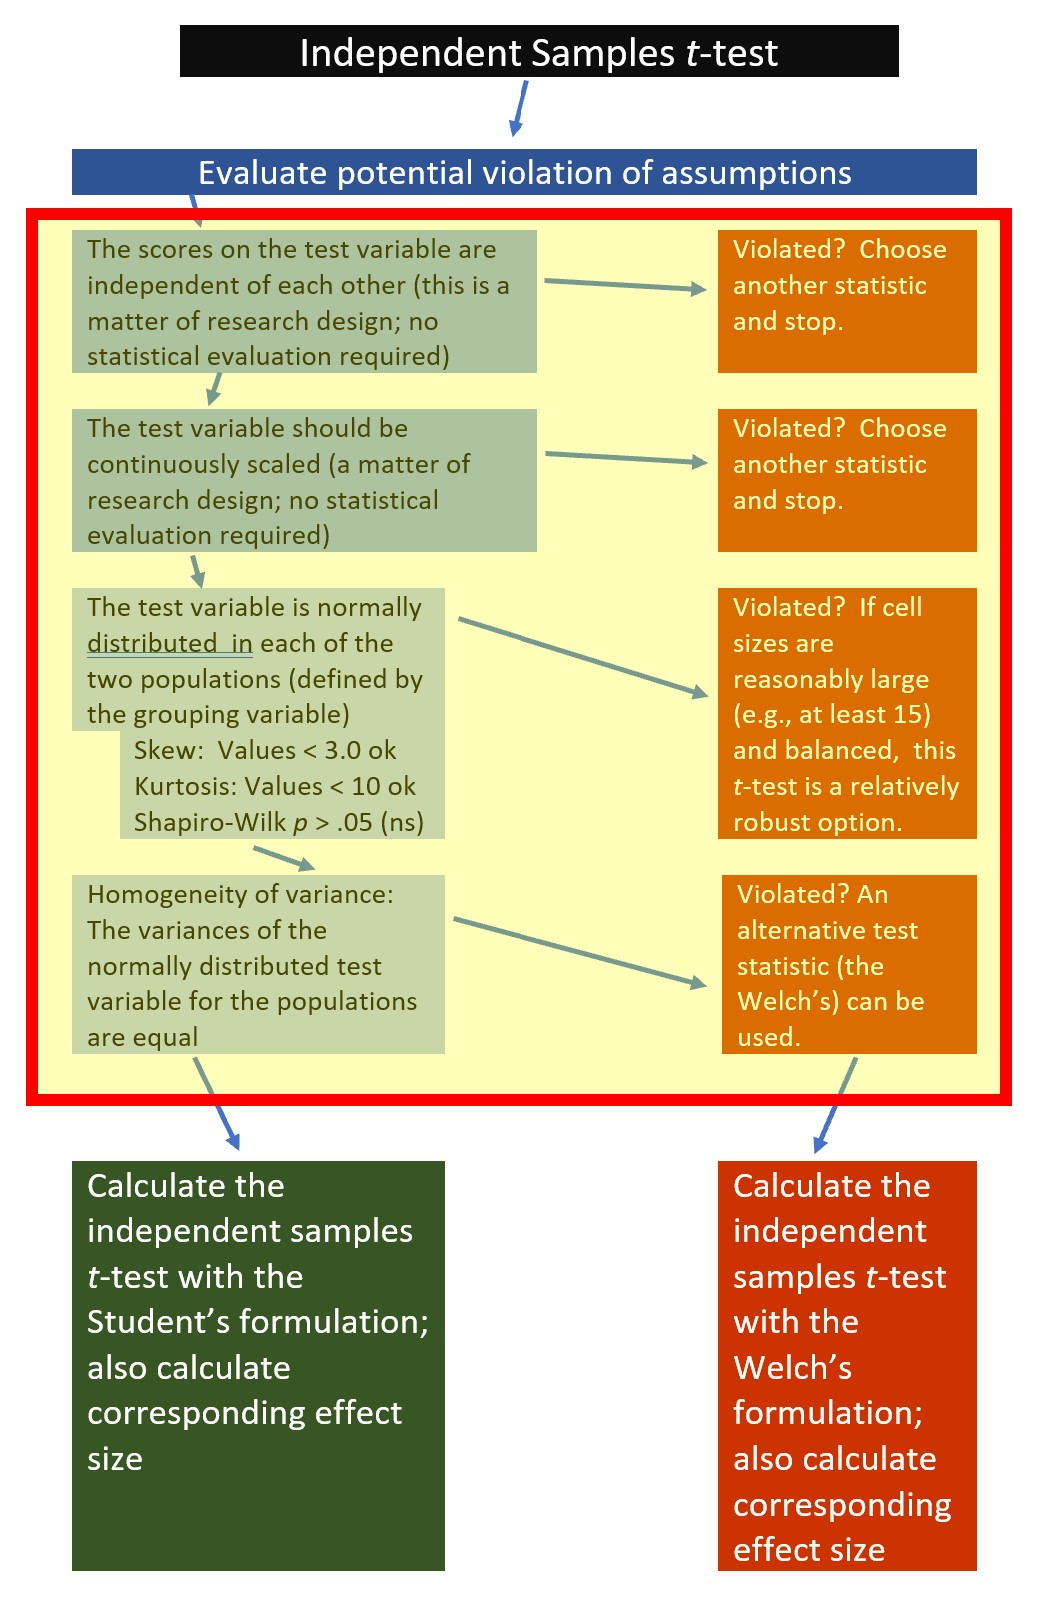
\includegraphics{images/ttests/IndSampleAssmptns.jpg}
\caption{The workflow for the one sample \emph{t}-test highlighting the evaluation of assumptions section}
\end{figure}

All statistical tests have some assumptions about the data. The independent-samples \emph{t}-test has four:

\begin{itemize}
\tightlist
\item
  The scores on the test variable as independent of each other. This is a research design issue and the independent-samples \emph{t}-test is not robust to violating this assumption.

  \begin{itemize}
  \tightlist
  \item
    If physicians' verbal communication was evaluated and reported for more than one patient, this vignette would violate the assumption of the independent samples \emph{t}-test. For the sake of simplicity, let's presume that each was evaluated on verbal communication for only one patient. If the research scenario was such that physicians contributed multiple datapoints a potential analytic choice that is robust to such a violation is \href{https://lhbikos.github.io/MultilevelModeling/}{multilevel modeling}.
  \end{itemize}
\item
  The test variable should be continuously scaled. This is also a matter of research design and no statistical analysis is required.

  \begin{itemize}
  \tightlist
  \item
    Our test variable is an evaluation of verbal interactions; this is continuously scaled and has the properties of \emph{interval}-level data.
  \end{itemize}
\item
  The test variable is normally distributed. We can check this several ways:

  \begin{itemize}
  \tightlist
  \item
    visually with histograms (perhaps with superimposed curves) and boxplots,
  \item
    calculation of skew and kurtosis values,
  \item
    calculation of the Shapiro-Wilk test of normality
  \end{itemize}
\item
  The variances of the normally distributed test variable for both levels of the grouping factor are equal. This is called the homogeneity of variance test and is easily calculated with a Levene's test of homogeneity of variance.
\end{itemize}

\hypertarget{is-the-dependent-variable-normally-distributed-at-each-level-of-the-grouping-variable}{%
\subsubsection{Is the dependent variable normally distributed at each level of the grouping variable?}\label{is-the-dependent-variable-normally-distributed-at-each-level-of-the-grouping-variable}}

We can begin to evaluate the assumption of normality by obtaining the descriptive statistics with the \emph{describe()} function from the \emph{psych} package.

\begin{Shaded}
\begin{Highlighting}[]
\NormalTok{psych}\SpecialCharTok{::}\FunctionTok{describe}\NormalTok{(dfIndSamples}\SpecialCharTok{$}\NormalTok{Verbal, }\AttributeTok{type =} \DecValTok{1}\NormalTok{)  }\CommentTok{\#type=1 produces the type of skew and kurtosis associated with Kline\textquotesingle{}s interpretive guidelines}
\end{Highlighting}
\end{Shaded}

\begin{verbatim}
   vars  n mean   sd median trimmed  mad  min   max range skew kurtosis   se
X1    1 66 8.25 3.14   7.93     8.2 3.08 0.35 19.31 18.96 0.44     1.34 0.39
\end{verbatim}

From this, we learn that the overall verbal mean is 8.25 with a standard deviation of 3.14. The values for skew (0.44) and kurtosis (1.34) fall below the areas of concern (below the absolute value of 3 for skew; below the absolute values of 10 for kurtosis) identified by Kline \citeyearpar{kline_data_2016}.

Recall that one of the assumptions for independent samples \emph{t}-test is that the variable of interest is normally distributed within each level of the grouping variable. The \emph{describeBy()} function in the \emph{psych} package allows us to obtain these skew and kurtosis at both levels of the grouping variable.

If we feed the function the entire df, it will give us results for each level of PatientRace for each variable, including variables for which such disaggregation is nonsensible (i.e., ID, PatientRace). If we had a large df, we might want to create a tiny df that only includes our variable(s) of interest. For now, it is not problematic to include all the variables.

\begin{Shaded}
\begin{Highlighting}[]
\NormalTok{psych}\SpecialCharTok{::}\FunctionTok{describeBy}\NormalTok{(dfIndSamples }\SpecialCharTok{\textasciitilde{}}\NormalTok{ PatientRace, }\AttributeTok{mat =} \ConstantTok{TRUE}\NormalTok{, }\AttributeTok{type =} \DecValTok{1}\NormalTok{)}
\end{Highlighting}
\end{Shaded}

\begin{verbatim}
              item group1 vars  n      mean        sd    median   trimmed
ID*1             1  Black    1 33 17.000000 9.6695398 17.000000 17.000000
ID*2             2  White    1 33 50.000000 9.6695398 50.000000 50.000000
PatientRace*1    3  Black    2 33  1.000000 0.0000000  1.000000  1.000000
PatientRace*2    4  White    2 33  2.000000 0.0000000  2.000000  2.000000
Verbal1          5  Black    3 33  7.614884 2.9854116  7.693516  7.733412
Verbal2          6  White    3 33  8.891483 3.2032222  7.979546  8.606615
Nonverbal1       7  Black    4 33  2.943125 0.9251164  2.885724  2.931841
Nonverbal2       8  White    4 33  2.965472 0.7001442  2.936787  2.995131
                     mad        min       max     range       skew   kurtosis
ID*1          11.8608000  1.0000000 33.000000 32.000000  0.0000000 -1.2022059
ID*2          11.8608000 34.0000000 66.000000 32.000000  0.0000000 -1.2022059
PatientRace*1  0.0000000  1.0000000  1.000000  0.000000        NaN        NaN
PatientRace*2  0.0000000  2.0000000  2.000000  0.000000        NaN        NaN
Verbal1        2.9075794  0.3507447 13.011100 12.660355 -0.3705014 -0.1377654
Verbal2        3.2861809  4.5891699 19.311207 14.722037  1.0651306  1.5382575
Nonverbal1     0.9185825  0.8333731  5.000000  4.166627  0.1204796  0.1380025
Nonverbal2     0.5560620  1.1311619  4.350886  3.219724 -0.4338806  0.3937160
                     se
ID*1          1.6832508
ID*2          1.6832508
PatientRace*1 0.0000000
PatientRace*2 0.0000000
Verbal1       0.5196935
Verbal2       0.5576094
Nonverbal1    0.1610421
Nonverbal2    0.1218795
\end{verbatim}

In this analysis we are interested in the verbal variable. We see that patients who are Black received verbal interactions from physicians that were quantified by a mean score of 7.61 (\emph{SD} = 2.99); physicians' scores for White patients were 8.89 (\emph{SD} = 3.20). Skew and kurtosis values for the verbal ratings with Black patients were -.37 and -.14, respectively. They were 1.07 and 1.54 for White patients. As before, these fall well below the absolute values of 3 (skew) and 10 (kurtosis) that are considered to be concerning.

Beyond skew and kurtosis, we can formally test for deviations from normality with a Shapiro-Wilk. The script below first groups the data by PatientRace and then applies the \emph{rstatix::shapiro\_test()}. We want the results to be non-significant.

\begin{Shaded}
\begin{Highlighting}[]
\FunctionTok{library}\NormalTok{(tidyverse)  }\CommentTok{\#opening this package so I can use the pipes}
\end{Highlighting}
\end{Shaded}

\begin{verbatim}
-- Attaching core tidyverse packages ------------------------ tidyverse 2.0.0 --
v dplyr     1.1.2     v readr     2.1.4
v forcats   1.0.0     v stringr   1.5.0
v ggplot2   3.4.2     v tibble    3.2.1
v lubridate 1.9.2     v tidyr     1.3.0
v purrr     1.0.1     
-- Conflicts ------------------------------------------ tidyverse_conflicts() --
x dplyr::filter() masks stats::filter()
x dplyr::lag()    masks stats::lag()
i Use the conflicted package (<http://conflicted.r-lib.org/>) to force all conflicts to become errors
\end{verbatim}

\begin{Shaded}
\begin{Highlighting}[]
\NormalTok{shapiro }\OtherTok{\textless{}{-}}\NormalTok{ dfIndSamples }\SpecialCharTok{\%\textgreater{}\%}
    \FunctionTok{group\_by}\NormalTok{(PatientRace) }\SpecialCharTok{\%\textgreater{}\%}
\NormalTok{    rstatix}\SpecialCharTok{::}\FunctionTok{shapiro\_test}\NormalTok{(Verbal)}
\NormalTok{shapiro}
\end{Highlighting}
\end{Shaded}

\begin{verbatim}
# A tibble: 2 x 4
  PatientRace variable statistic      p
  <fct>       <chr>        <dbl>  <dbl>
1 Black       Verbal       0.977 0.677 
2 White       Verbal       0.922 0.0204
\end{verbatim}

The Shapiro-Wilk test of normality indicated that the dependent variable, evaluation of verbal interaction with the patient was normally distributed within Black patients \((W = 0.977, p = 0.677)\), but not within White patients \((W = 0.922, p = 0.020\). That is, the distribution of verbal communication scores for physicians attending to White patients was statistically significantly different from a normal distribution.

Should we be concerned? A general rule of thumb is that when cell sizes are larger than 15 the independent \emph{t}-test should be relatively robust to violations of normality \citep{green_using_2017}.

\hypertarget{are-the-variances-of-the-dependent-variable-similar-across-the-levels-of-the-grouping-factor}{%
\subsubsection{Are the variances of the dependent variable similar across the levels of the grouping factor?}\label{are-the-variances-of-the-dependent-variable-similar-across-the-levels-of-the-grouping-factor}}

One of the assumptions of the independent samples \emph{t}-test is that the variances of the dependent variable (verbal communication) are similar for both levels of the PatientRace factor. We can use the Levene's test to do this. We want this value to be non-significant \((p > .05)\). If violated, we we can use the Welch's test because it is robust to the violation of the homogeneity of variance.

Using \emph{rstatix::levene\_test()}, we simply need to point to the data, provide a ``formula'' in the form of ``dependent variable by grouping variable,'' and specify about how to center the data. The median is a commonly used because it provides a more robust test.

\begin{Shaded}
\begin{Highlighting}[]
\NormalTok{rstatix}\SpecialCharTok{::}\FunctionTok{levene\_test}\NormalTok{(dfIndSamples, Verbal }\SpecialCharTok{\textasciitilde{}}\NormalTok{ PatientRace, }\AttributeTok{center =}\NormalTok{ median)}
\end{Highlighting}
\end{Shaded}

\begin{verbatim}
# A tibble: 1 x 4
    df1   df2 statistic     p
  <int> <int>     <dbl> <dbl>
1     1    64    0.0398 0.843
\end{verbatim}

The results of the Levene's test are presented as an \emph{F} statistic. We'll get to \emph{F} distributions in the next chapter. For now, it is just important to know how to report and interpret them:

\begin{itemize}
\tightlist
\item
  Degrees of freedom are 1 and 64
\item
  The value of the \emph{F} statistic is 0.039
\item
  The \emph{p} value is 0.843 (i.e., greater than .05)
\end{itemize}

Happily, our Levene's result is \((F[1, 64] = 0.039, p = 0.843)\) not significant. Because \emph{p} is greater than .05, we have not violated the homogeneity of variance assumption. That is to say, the variance in the patient race groups is not statistically significantly different from each other. We can use the regular (Student's) formulation of the \emph{t}-test for independent samples.

\hypertarget{apa-style-write-up-of-testing-the-assumptions}{%
\subsubsection{APA style write-up of testing the assumptions}\label{apa-style-write-up-of-testing-the-assumptions}}

My practice is to create APA style drafts of the different sections of the analysis as I work along. Here's how I might capture our evaluation of the statistical assumptions:

\begin{quote}
We began by analyzing the data to see if it met the statistical assumptions for analysis with an independent samples \emph{t}-test. One assumption is that the dependent variable be normally distributed within the both levels of the grouping variable. We evaluated skew and kurtosis using Kline's \citeyearpar{kline_data_2016} guidelines of the absolute values of 3 (skew) and 10 (kurtosis). Our results were well-within these boundary conditions. Specifically, the verbal ratings of physicians with Black patients were -.37 and -.14 for skew and kurtosis, respectively; they were 1.07 and 1.54 for White patients. The Shapiro-Wilk test of normality indicated that the dependent variable was normally distributed within Black patients \((W = 0.977, p = 0.677)\), but not within White patients \((W = 0.922, p = 0.020)\). That is, the distribution of verbal communication scores for physicians attending to White patients was statistically significantly different from a normal distribution. Results of Levene's homogeneity of variance test suggested that the variance in each of the patient race groups was not statistically significantly different from each other \((F[1, 64] = 0.039, p = 0.843)\). Because the independent samples \emph{t}-test is relatively robust to violations of normality when samples sizes have at least 15 participants per cell \citep{green_using_2017} and there was no violation of the homogeneity of variance assumption we proceded with the Student's formulation of the \emph{t}-test for independent samples.
\end{quote}

Odds are, owing to space limitations in journals, you would not provide this much detail about an independent samples \emph{t}-test in an empirical manuscript. I am encouraging you to do so as you work through these chapters because it is good practice for thinking through the logic and sequencing of statistics as well as writing results in APA style.

\hypertarget{computing-the-independent-samples-t-test}{%
\subsection{\texorpdfstring{Computing the Independent Samples \emph{t}-Test}{Computing the Independent Samples t-Test}}\label{computing-the-independent-samples-t-test}}

We are ready to compute the independent samples \emph{t}-test.

\begin{figure}
\centering
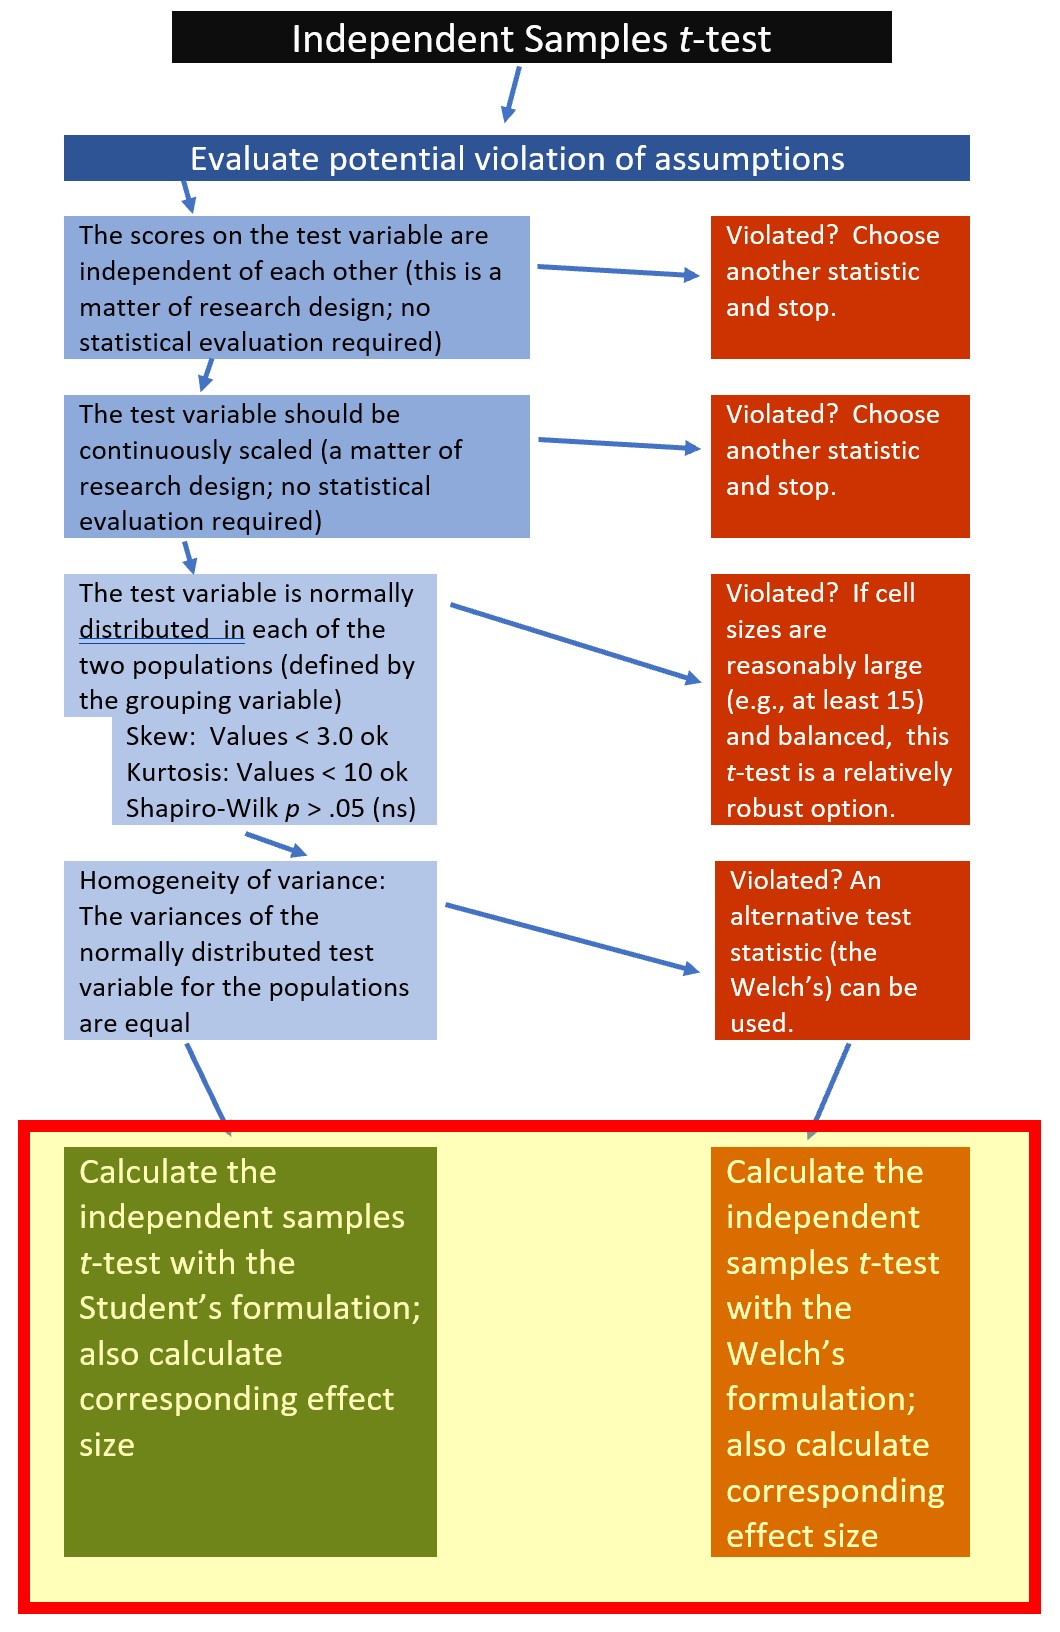
\includegraphics{images/ttests/IntSampT.jpg}
\caption{A colorful image of a workflow for the paired samples \emph{t}-test focusing on the computation of the t-test}
\end{figure}

Calculating an independent samples \emph{t}-test is possible through base R and a number of packages. Kassambara's \citeyearpar{kassambara_pipe-friendly_nodate} \emph{rstatix} package is one we can use for all of the \emph{t}-test and ANOVA problems that we will work. I like it for several reasons. First, it was designed to be ``pipe-friendly'' in a manner that is consistent with the \emph{tidyverse} approach to working in R and there are numerous tutorials. Additionally, \emph{rstatix} objects work well with \emph{ggpubr}, one of my favorite packages for graphing data and results.

In the script below:

\begin{itemize}
\tightlist
\item
  the first element points to the dataframe
\item
  the second element provides a ``formula''

  \begin{itemize}
  \tightlist
  \item
    we are predicting ``Verbal'' from ``PatientRace''
  \end{itemize}
\item
  the third element, ``var.equal=TRUE'' means that we are using Student's formulation (because we did not violate the homogeneity of variance assumption)
\item
  specifying ``detailed = TRUE'' will produce the 95\% confidence interval around the difference in the two means
\end{itemize}

\begin{Shaded}
\begin{Highlighting}[]
\NormalTok{rstatix}\SpecialCharTok{::}\FunctionTok{t\_test}\NormalTok{(dfIndSamples, Verbal }\SpecialCharTok{\textasciitilde{}}\NormalTok{ PatientRace, }\AttributeTok{var.equal =} \ConstantTok{TRUE}\NormalTok{, }\AttributeTok{detailed =} \ConstantTok{TRUE}\NormalTok{)}
\end{Highlighting}
\end{Shaded}

\begin{verbatim}
# A tibble: 1 x 15
  estimate estimate1 estimate2 .y.    group1 group2    n1    n2 statistic      p
*    <dbl>     <dbl>     <dbl> <chr>  <chr>  <chr>  <int> <int>     <dbl>  <dbl>
1    -1.28      7.61      8.89 Verbal Black  White     33    33     -1.67 0.0989
# i 5 more variables: df <dbl>, conf.low <dbl>, conf.high <dbl>, method <chr>,
#   alternative <chr>
\end{verbatim}

From this output we can start to draft our \emph{t} string: \(t(64) = -1.675, p = 0.099, CI95(-2.80, 0.25)\).

Separately, we must request the effect size. Earlier in the lesson we calculated both Cohen's \emph{d} and eta-squared. Unfortunately, the \emph{rstatix} package only offers the Cohen's \emph{d} for \emph{t}-tests. If you wanted an eta-squared, it would be easy enough to hand-calculate (or obtain from another R package).

\begin{Shaded}
\begin{Highlighting}[]
\NormalTok{rstatix}\SpecialCharTok{::}\FunctionTok{cohens\_d}\NormalTok{(dfIndSamples, Verbal }\SpecialCharTok{\textasciitilde{}}\NormalTok{ PatientRace, }\AttributeTok{var.equal =} \ConstantTok{TRUE}\NormalTok{)}
\end{Highlighting}
\end{Shaded}

\begin{verbatim}
# A tibble: 1 x 7
  .y.    group1 group2 effsize    n1    n2 magnitude
* <chr>  <chr>  <chr>    <dbl> <int> <int> <ord>    
1 Verbal Black  White   -0.412    33    33 small    
\end{verbatim}

We can update our \emph{t} string to include the effect size: \(t(64) = -1.675, p = 0.099, CI95(-2.80, 0.25), d = -0.412\)

What does this mean? Our result is not-significant. Our estimate of the difference in verbal communication ratings when physicians interacted with Black and White patients was -1.675. We are 95\% confident that that true mean difference is as low as -2.80 or as high as 0.25. Because the confidence interval crosses zero, we cannot be certain that the true difference is zero. This is consistent with the non-significant \emph{p} value and effect size. Our output even tells us that the \emph{d} of -0.41 is small.

\hypertarget{what-if-we-had-violated-the-homogeneity-of-variance-assumption}{%
\subsection{What if we had violated the homogeneity of variance assumption?}\label{what-if-we-had-violated-the-homogeneity-of-variance-assumption}}

Earlier we used the Levene's test to examine the homogeneity of variance assumption. If we had violated it, the Welch's formulation of the independent sample \emph{t}-test is available to us. The \emph{rstatix} package makes this easy. We simply change the \emph{var.equal} to \emph{FALSE}. This will produce the Welch's alternative, which takes into consideration violations of the homogeneity of variance assumption. Conveniently, ``Student's'' or ``Welch's'' will serve as the first row of the output.

\begin{Shaded}
\begin{Highlighting}[]
\NormalTok{rstatix}\SpecialCharTok{::}\FunctionTok{t\_test}\NormalTok{(dfIndSamples, Verbal }\SpecialCharTok{\textasciitilde{}}\NormalTok{ PatientRace, }\AttributeTok{var.equal =} \ConstantTok{FALSE}\NormalTok{,}
    \AttributeTok{detailed =} \ConstantTok{TRUE}\NormalTok{)}
\end{Highlighting}
\end{Shaded}

\begin{verbatim}
# A tibble: 1 x 15
  estimate estimate1 estimate2 .y.    group1 group2    n1    n2 statistic      p
*    <dbl>     <dbl>     <dbl> <chr>  <chr>  <chr>  <int> <int>     <dbl>  <dbl>
1    -1.28      7.61      8.89 Verbal Black  White     33    33     -1.67 0.0989
# i 5 more variables: df <dbl>, conf.low <dbl>, conf.high <dbl>, method <chr>,
#   alternative <chr>
\end{verbatim}

Likely because of the similarity of the standard deviations associated with each level of patient race and our equal cell sizes, this changes nothing about our conclusion. Note that the degrees of freedom in the Student's \emph{t}-test analysis (the first one) was 64; in the Welch's version, the degrees of freedom is 63.685. It is this change that, when the homogeneity of variance assumption is violated, can make the Welch's results more conservative (i.e., less likely to have a statistically significant result).

\hypertarget{apa-style-results-1}{%
\section{APA Style Results}\label{apa-style-results-1}}

Putting it altogether, here is an APA Style results section:

\begin{quote}
An independent samples \emph{t}-test was conducted to evaluate the hypothesis that there would be differences between the quality of physicians' verbal communication depending on whether the patient's race (Black, White).
\end{quote}

\begin{quote}
We began by analyzing the data to see if it met the statistical assumptions for analysis with an independent samples \emph{t}-test. One assumption is that the dependent variable be normally distributed within the both levels of the grouping variable. We evaluated skew and kurtosis using Kline's \citeyearpar{kline_data_2016} guidelines of the absolute values of 3 (skew) and 10 (kurtosis). Our results were well-within these boundary conditions. Specifically, the verbal ratings of physicians with Black patients were -.37 and -.14 for skew and kurtosis, respectively; they were 1.07 and 1.54 for White patients. The Shapiro-Wilk test of normality indicated that the dependent variable was normally distributed within Black patients \((W = 0.977, p = 0.677)\), but not within White patients \((W = 0.922, p = 0.020\). That is, the distribution of verbal communication scores for physicians attending to White patients was statistically significantly different from a normal distribution. Results of Levene's homogeneity of variance test suggested that the variance in each of the patient race groups was not statistically significantly different from each other \((F[1, 64] = 0.039, p = 0.843)\). Because the independent samples \emph{t}-test is relatively robust to violations of normality when samples sizes have at least 15 participants per cell \citep{green_using_2017} and there was no violation of the homogeneity of variance assumption we proceded with the Student's formulation of the \emph{t}-test for independent samples.
\end{quote}

\begin{quote}
Results of the independent samples \emph{t}-test was nonsignificant, \(t(64) = -1.675, p = .099, d = 0.412\). The 95\% confidence interval for the difference in means ranged from -2.799 to 0.246. Means and standard deviations are presented in Table 1; the results are illustrated in Figure 1.
\end{quote}

\begin{Shaded}
\begin{Highlighting}[]
\NormalTok{apaTables}\SpecialCharTok{::}\FunctionTok{apa.1way.table}\NormalTok{(PatientRace, Verbal, dfIndSamples)}
\end{Highlighting}
\end{Shaded}

\begin{verbatim}


Descriptive statistics for Verbal as a function of PatientRace.  

 PatientRace    M   SD
       Black 7.61 2.99
       White 8.89 3.20

Note. M and SD represent mean and standard deviation, respectively.
 
\end{verbatim}

The figure we created earlier in the lesson would be sufficient for a journal article. However, using \emph{rstatix} in combination with \emph{ggpubbr} can be quite powerful. The result can be a figure that includes the \emph{t}-test results and ``significance bars.'' To do this, we first need to re-run the \emph{rstatix::t\_test}, but adding to it by

\begin{itemize}
\tightlist
\item
  including ``add\_significance()'' script after the pipe, and
\item
  saving it as an object, which I'm naming ``pair.test.''
\end{itemize}

We could have done this in the initial run (but I didn't want to make the test-statistic unnecessarily confusing).

\begin{Shaded}
\begin{Highlighting}[]
\NormalTok{ind.test }\OtherTok{\textless{}{-}}\NormalTok{ rstatix}\SpecialCharTok{::}\FunctionTok{t\_test}\NormalTok{(dfIndSamples, Verbal }\SpecialCharTok{\textasciitilde{}}\NormalTok{ PatientRace, }\AttributeTok{var.equal =} \ConstantTok{TRUE}\NormalTok{,}
    \AttributeTok{detailed =} \ConstantTok{TRUE}\NormalTok{) }\SpecialCharTok{\%\textgreater{}\%}
\NormalTok{    rstatix}\SpecialCharTok{::}\FunctionTok{add\_significance}\NormalTok{()}
\NormalTok{ind.test}
\end{Highlighting}
\end{Shaded}

\begin{verbatim}
# A tibble: 1 x 16
  estimate estimate1 estimate2 .y.    group1 group2    n1    n2 statistic      p
     <dbl>     <dbl>     <dbl> <chr>  <chr>  <chr>  <int> <int>     <dbl>  <dbl>
1    -1.28      7.61      8.89 Verbal Black  White     33    33     -1.67 0.0989
# i 6 more variables: df <dbl>, conf.low <dbl>, conf.high <dbl>, method <chr>,
#   alternative <chr>, p.signif <chr>
\end{verbatim}

Next, we update the earlier boxplot code with the results from our statistical analyses:

\begin{Shaded}
\begin{Highlighting}[]
\NormalTok{ind.box }\OtherTok{\textless{}{-}}\NormalTok{ ggpubr}\SpecialCharTok{::}\FunctionTok{ggboxplot}\NormalTok{(dfIndSamples, }\AttributeTok{x =} \StringTok{"PatientRace"}\NormalTok{, }\AttributeTok{y =} \StringTok{"Verbal"}\NormalTok{,}
    \AttributeTok{color =} \StringTok{"PatientRace"}\NormalTok{, }\AttributeTok{palette =} \FunctionTok{c}\NormalTok{(}\StringTok{"\#00AFBB"}\NormalTok{, }\StringTok{"\#FC4E07"}\NormalTok{), }\AttributeTok{add =} \StringTok{"jitter"}\NormalTok{,}
    \AttributeTok{title =} \StringTok{"Figure 1. Physician Verbal Engagement as a Function of Patient Race"}\NormalTok{)}
\NormalTok{ind.test }\OtherTok{\textless{}{-}}\NormalTok{ ind.test }\SpecialCharTok{\%\textgreater{}\%}
\NormalTok{    rstatix}\SpecialCharTok{::}\FunctionTok{add\_xy\_position}\NormalTok{(}\AttributeTok{x =} \StringTok{"PatientRace"}\NormalTok{)  }\CommentTok{\#autocomputes p{-}value labels positions}
\NormalTok{ind.box }\OtherTok{\textless{}{-}}\NormalTok{ ind.box }\SpecialCharTok{+}\NormalTok{ ggpubr}\SpecialCharTok{::}\FunctionTok{stat\_pvalue\_manual}\NormalTok{(ind.test, }\AttributeTok{label =} \StringTok{"p.signif"}\NormalTok{,}
    \AttributeTok{tip.length =} \FloatTok{0.02}\NormalTok{, }\AttributeTok{hide.ns =} \ConstantTok{FALSE}\NormalTok{, }\AttributeTok{y.position =} \FunctionTok{c}\NormalTok{(}\DecValTok{18}\NormalTok{)) }\SpecialCharTok{+} \FunctionTok{labs}\NormalTok{(}\AttributeTok{subtitle =}\NormalTok{ rstatix}\SpecialCharTok{::}\FunctionTok{get\_test\_label}\NormalTok{(ind.test,}
    \AttributeTok{detailed =} \ConstantTok{TRUE}\NormalTok{))  }\CommentTok{\#adds t{-}test results}

\NormalTok{ind.box}
\end{Highlighting}
\end{Shaded}

\includegraphics{05-tIndSample_files/figure-latex/unnamed-chunk-27-1.pdf} Between the \emph{rstatix} and \emph{ggpubr} tools, there is a great deal of flexibility in creating figures. Determining which figure is best will likely depend on your outlet, your audience, your goals, and your personal preferences. For example, a print journal might prefer a black-and-white figure (with no fill in the boxes). This is accomplished easily enough by removing (or, hashtagging out) the ``color'' and ``palette'' arguments.

\hypertarget{power-in-independent-samples-t-tests}{%
\section{\texorpdfstring{Power in Independent Samples \emph{t}-tests}{Power in Independent Samples t-tests}}\label{power-in-independent-samples-t-tests}}

Researchers often use power analysis packages to estimate the sample size needed to detect a statistically significant effect, if, in fact, there is one. Utilized another way, these tools allows us to determine the probability of detecting an effect of a given size with a given level of confidence. If the probability is unacceptably low, we may want to revise or stop. A helpful overview of power as well as guidelines for how to use the \emph{pwr} package can be found at a \href{https://www.statmethods.net/stats/power.html}{Quick-R website} \citep{kabacoff_power_2017}.

In Champely's \emph{pwr} package, we can conduct a power analysis for a variety of designs, including the independent samples \emph{t}-test that we worked in this lesson. There are a number of interrelating elements of power:

\begin{itemize}
\tightlist
\item
  Sample size, \emph{n} refers to the number of observations in each group; our vignette had 33
\item
  \emph{d} refers to the difference between means divided by the pooled standard deviation; we can use the value of Cohen's \emph{d} for this
\item
  \emph{power} refers to the power of a statistical test; conventionally it is set at .80
\item
  \emph{sig.level} refers to our desired alpha level; conventionally it is set at .05
\item
  \emph{type} indicates the type of test we ran; this was ``two.sample''
\item
  \emph{alternative} refers to whether the hypothesis is non-directional/two-tailed (``two.sided'') or directional/one-tailed(``less'' or ``greater'')
\end{itemize}

In this script, we must specify \emph{all-but-one} parameter; the remaining parameter must be defined as NULL. R will calculate the value for the missing parameter.

When we conduct a ``power analysis'' (i.e., the likelihood of a hypothesis test detecting an effect if there is one), we specify, ``power=NULL''. Using the data from our results, we learn from this first run, that our statistical power was 0.38. That is, given the value of the mean difference (1.276) we had a 38\% chance of detecting a statistically significant effect if there was one. This is consistent with our non-significant result.

\begin{Shaded}
\begin{Highlighting}[]
\NormalTok{pwr}\SpecialCharTok{::}\FunctionTok{pwr.t.test}\NormalTok{(}\AttributeTok{d =} \SpecialCharTok{{-}}\FloatTok{0.412}\NormalTok{, }\AttributeTok{n =} \DecValTok{33}\NormalTok{, }\AttributeTok{power =} \ConstantTok{NULL}\NormalTok{, }\AttributeTok{sig.level =} \FloatTok{0.05}\NormalTok{, }\AttributeTok{type =} \StringTok{"two.sample"}\NormalTok{,}
    \AttributeTok{alternative =} \StringTok{"two.sided"}\NormalTok{)}
\end{Highlighting}
\end{Shaded}

\begin{verbatim}

     Two-sample t test power calculation 

              n = 33
              d = 0.412
      sig.level = 0.05
          power = 0.3778572
    alternative = two.sided

NOTE: n is number in *each* group
\end{verbatim}

Researchers frequently use these tools to estimate the sample size required to obtain a statistically significant effect. In these scenarios we set \emph{n} to \emph{NULL}. Using the results from the simulation of our research vignette, you can see that we would have needed 93 individuals (per group; 186 total) for the \emph{p} value to be \textless{} .05.

\begin{Shaded}
\begin{Highlighting}[]
\NormalTok{pwr}\SpecialCharTok{::}\FunctionTok{pwr.t.test}\NormalTok{(}\AttributeTok{d =} \SpecialCharTok{{-}}\FloatTok{0.412}\NormalTok{, }\AttributeTok{n =} \ConstantTok{NULL}\NormalTok{, }\AttributeTok{power =} \FloatTok{0.8}\NormalTok{, }\AttributeTok{sig.level =} \FloatTok{0.05}\NormalTok{, }\AttributeTok{type =} \StringTok{"two.sample"}\NormalTok{,}
    \AttributeTok{alternative =} \StringTok{"two.sided"}\NormalTok{)}
\end{Highlighting}
\end{Shaded}

\begin{verbatim}

     Two-sample t test power calculation 

              n = 93.44893
              d = 0.412
      sig.level = 0.05
          power = 0.8
    alternative = two.sided

NOTE: n is number in *each* group
\end{verbatim}

Given that we had a non-significant result, this is not surprising. None-the-less, let's try it again. Below I will re-simulate the data for the verbal scores and change only the sample size:

\begin{Shaded}
\begin{Highlighting}[]
\FunctionTok{set.seed}\NormalTok{(}\DecValTok{230525}\NormalTok{)}
\CommentTok{\# sample size, M, and SD for Black then White patients}
\NormalTok{rVerbal }\OtherTok{\textless{}{-}} \FunctionTok{c}\NormalTok{(}\FunctionTok{rnorm}\NormalTok{(}\DecValTok{93}\NormalTok{, }\AttributeTok{mean =} \FloatTok{8.37}\NormalTok{, }\AttributeTok{sd =} \FloatTok{3.36}\NormalTok{), }\FunctionTok{rnorm}\NormalTok{(}\DecValTok{93}\NormalTok{, }\AttributeTok{mean =} \FloatTok{8.41}\NormalTok{,}
    \AttributeTok{sd =} \FloatTok{3.21}\NormalTok{))}
\CommentTok{\# set upper bound}
\NormalTok{rVerbal[rVerbal }\SpecialCharTok{\textgreater{}} \DecValTok{27}\NormalTok{] }\OtherTok{\textless{}{-}} \DecValTok{3}
\CommentTok{\# set lower bound}
\NormalTok{rVerbal[rVerbal }\SpecialCharTok{\textless{}} \DecValTok{0}\NormalTok{] }\OtherTok{\textless{}{-}} \DecValTok{0}
\CommentTok{\# sample size, M, and SD for Black then White patients}
\NormalTok{rNonverbal }\OtherTok{\textless{}{-}} \FunctionTok{c}\NormalTok{(}\FunctionTok{rnorm}\NormalTok{(}\DecValTok{93}\NormalTok{, }\AttributeTok{mean =} \FloatTok{2.68}\NormalTok{, }\AttributeTok{sd =} \FloatTok{0.84}\NormalTok{), }\FunctionTok{rnorm}\NormalTok{(}\DecValTok{93}\NormalTok{, }\AttributeTok{mean =} \FloatTok{2.93}\NormalTok{,}
    \AttributeTok{sd =} \FloatTok{0.77}\NormalTok{))}
\CommentTok{\# set upper bound}
\NormalTok{rNonverbal[rNonverbal }\SpecialCharTok{\textgreater{}} \DecValTok{5}\NormalTok{] }\OtherTok{\textless{}{-}} \DecValTok{5}
\CommentTok{\# set lower bound}
\NormalTok{rNonverbal[rNonverbal }\SpecialCharTok{\textless{}} \DecValTok{0}\NormalTok{] }\OtherTok{\textless{}{-}} \DecValTok{0}

\NormalTok{rID }\OtherTok{\textless{}{-}} \FunctionTok{factor}\NormalTok{(}\FunctionTok{seq}\NormalTok{(}\DecValTok{1}\NormalTok{, }\DecValTok{186}\NormalTok{))}
\CommentTok{\# name factors and identify how many in each group; should be in same}
\CommentTok{\# order as first row of script}
\NormalTok{rPatientRace }\OtherTok{\textless{}{-}} \FunctionTok{c}\NormalTok{(}\FunctionTok{rep}\NormalTok{(}\StringTok{"Black"}\NormalTok{, }\DecValTok{93}\NormalTok{), }\FunctionTok{rep}\NormalTok{(}\StringTok{"White"}\NormalTok{, }\DecValTok{93}\NormalTok{))}
\CommentTok{\# groups the 3 variables into a single df: ID\#, DV, condition}
\NormalTok{rdfIndSamples }\OtherTok{\textless{}{-}} \FunctionTok{data.frame}\NormalTok{(rID, rPatientRace, rVerbal, rNonverbal)}

\NormalTok{rdfIndSamples}\SpecialCharTok{$}\NormalTok{rPatientRace }\OtherTok{\textless{}{-}} \FunctionTok{factor}\NormalTok{(rdfIndSamples}\SpecialCharTok{$}\NormalTok{rPatientRace, }\AttributeTok{levels =} \FunctionTok{c}\NormalTok{(}\StringTok{"Black"}\NormalTok{,}
    \StringTok{"White"}\NormalTok{))}
\end{Highlighting}
\end{Shaded}

\begin{Shaded}
\begin{Highlighting}[]
\NormalTok{rstatix}\SpecialCharTok{::}\FunctionTok{t\_test}\NormalTok{(rdfIndSamples, rVerbal }\SpecialCharTok{\textasciitilde{}}\NormalTok{ rPatientRace, }\AttributeTok{var.equal =} \ConstantTok{TRUE}\NormalTok{,}
    \AttributeTok{detailed =} \ConstantTok{TRUE}\NormalTok{)}
\end{Highlighting}
\end{Shaded}

\begin{verbatim}
# A tibble: 1 x 15
  estimate estimate1 estimate2 .y.    group1 group2    n1    n2 statistic      p
*    <dbl>     <dbl>     <dbl> <chr>  <chr>  <chr>  <int> <int>     <dbl>  <dbl>
1    0.852      9.02      8.17 rVerb~ Black  White     93    93      1.71 0.0884
# i 5 more variables: df <dbl>, conf.low <dbl>, conf.high <dbl>, method <chr>,
#   alternative <chr>
\end{verbatim}

\begin{Shaded}
\begin{Highlighting}[]
\NormalTok{rstatix}\SpecialCharTok{::}\FunctionTok{cohens\_d}\NormalTok{(rdfIndSamples, rVerbal }\SpecialCharTok{\textasciitilde{}}\NormalTok{ rPatientRace, }\AttributeTok{var.equal =} \ConstantTok{TRUE}\NormalTok{)}
\end{Highlighting}
\end{Shaded}

\begin{verbatim}
# A tibble: 1 x 7
  .y.     group1 group2 effsize    n1    n2 magnitude
* <chr>   <chr>  <chr>    <dbl> <int> <int> <ord>    
1 rVerbal Black  White    0.251    93    93 small    
\end{verbatim}

Curiously, our result is still not statistically significant: \(t(184) = 1.713, p = 0.088, d = 0.251, CI95[-0.129, 1.832]\). Given the closeness of our means (9.025, 8.173), this makes sense to me. Additionally, it does show us, though, how power is influenced by sample size. Holding all else equal, the larger the sample, the more likely we are to have a statistically significant result.

\hypertarget{practice-problems-3}{%
\section{Practice Problems}\label{practice-problems-3}}

The suggestions for homework differ in degree of complexity. I encourage you to start with a problem that feels ``do-able'' and then try at least one more problem that challenges you in some way. Regardless, your choices should meet you where you are (e.g., in terms of your self-efficacy for statistics, your learning goals, and competing life demands).

Additionally, please complete at least one set of \emph{hand calculations}, that is using the code demonstrated in the chapter to work through the formulas that compute the independent samples \emph{t}-test. At this stage in your learning, you may ignore any missingness in your dataset by excluding all rows with missing data in your variables of interest.

\hypertarget{problem-1-rework-the-research-vignette-as-demonstrated-but-change-the-random-seed-1}{%
\subsection{Problem \#1: Rework the research vignette as demonstrated, but change the random seed}\label{problem-1-rework-the-research-vignette-as-demonstrated-but-change-the-random-seed-1}}

If this topic feels a bit overwhelming, simply change the random seed in the data simulation of the research vignette, then rework the problem. This should provide minor changes to the data (maybe even in the second or third decimal point), but the results will likely be very similar. That said, don't be alarmed if what was non-significant in my working of the problem becomes significant. Our selection of \emph{p} \textless{} .05 (and the corresponding 95\% confidence interval) means that 5\% of the time there could be a difference in statistical significance.

\hypertarget{problem-2-rework-the-research-vignette-but-change-something-about-the-simulation-1}{%
\subsection{Problem \#2: Rework the research vignette, but change something about the simulation}\label{problem-2-rework-the-research-vignette-but-change-something-about-the-simulation-1}}

Rework the independent samples \emph{t}-test in the lesson by changing something else about the simulation. You might have noticed that my re-simulation of a smaller sample size did not produce a statistically significant result. You may wish to pick a value in between the primary lecture \emph{N} and the re-simulation to see what it takes to achieve statistical significance. Alternatively, you could specify different means and/or standard deviations.

\hypertarget{problem-3-rework-the-research-vignette-but-swap-one-or-more-variables}{%
\subsection{Problem \#3: Rework the research vignette, but swap one or more variables}\label{problem-3-rework-the-research-vignette-but-swap-one-or-more-variables}}

Use the simulated data, but select the nonverbal communication variables that were evaluated in the Elliott et al. \citeyearpar{elliott_differences_2016}study. Compare your results to those reported in the mansucript.

\hypertarget{problem-4-use-other-data-that-is-available-to-you}{%
\subsection{Problem \#4: Use other data that is available to you}\label{problem-4-use-other-data-that-is-available-to-you}}

Using data for which you have permission and access (e.g., IRB approved data you have collected or from your lab; data you simulate from a published article; data from an open science repository; data from other chapters in this OER), complete an independent samples \emph{t}-test.

\hypertarget{grading-rubric-1}{%
\subsection{Grading Rubric}\label{grading-rubric-1}}

Regardless which option(s) you chose, use the elements in the grading rubric to guide you through the practice.

\begin{longtable}[]{@{}
  >{\raggedright\arraybackslash}p{(\columnwidth - 4\tabcolsep) * \real{0.5493}}
  >{\centering\arraybackslash}p{(\columnwidth - 4\tabcolsep) * \real{0.2535}}
  >{\centering\arraybackslash}p{(\columnwidth - 4\tabcolsep) * \real{0.1972}}@{}}
\toprule\noalign{}
\begin{minipage}[b]{\linewidth}\raggedright
Assignment Component
\end{minipage} & \begin{minipage}[b]{\linewidth}\centering
Points Possible
\end{minipage} & \begin{minipage}[b]{\linewidth}\centering
Points Earned
\end{minipage} \\
\midrule\noalign{}
\endhead
\bottomrule\noalign{}
\endlastfoot
1. Narrate the research vignette, describing the variables and their role in the analysis & 5 & \_\_\_\_\_ \\
2. Simulate (or import) and format data & 5 & \_\_\_\_\_ \\
3. Evaluate statistical assumptions & 5 & \_\_\_\_\_ \\
4. Conduct an independent samples \emph{t}-test (with an effect size and 95\%CIs) & 5 & \_\_\_\_\_ \\
5. APA style results with table(s) and figure & 5 & \_\_\_\_\_ \\
6. Conduct power analyses to determine the power of the current study and a recommended sample size & 5 & \_\_\_\_\_ \\
7. Explanation to grader & 5 & \_\_\_\_\_ \\
\textbf{Totals} & 35 & \_\_\_\_\_ \\
\end{longtable}

\begin{longtable}[]{@{}
  >{\raggedright\arraybackslash}p{(\columnwidth - 4\tabcolsep) * \real{0.5833}}
  >{\centering\arraybackslash}p{(\columnwidth - 4\tabcolsep) * \real{0.2083}}
  >{\raggedright\arraybackslash}p{(\columnwidth - 4\tabcolsep) * \real{0.2083}}@{}}
\toprule\noalign{}
\begin{minipage}[b]{\linewidth}\raggedright
Hand Calculations
\end{minipage} & \begin{minipage}[b]{\linewidth}\centering
Points Poss
\end{minipage} & \begin{minipage}[b]{\linewidth}\raggedright
Points Earned
\end{minipage} \\
\midrule\noalign{}
\endhead
\bottomrule\noalign{}
\endlastfoot
1. Using traditional NHST (null hypothesis testing language), state your null and alternative hypotheses & 2 & \\
2. Using an R package or functions in base R, calculate the means and standard deviations for both levels of the dependent variable & 4 & \\
3. Calculate the SE used in the denominator of the \emph{t}-test & 4 & \\
4. Calculate the independent samples \emph{t}-test & 4 & \\
5. Identify the degrees of freedom associated with your \emph{t}-test & 2 & \\
6. Locate the test critical value for your test & 2 & \\
7. Is the \emph{t}-test statistically significant? Why or why not? & 2 & \\
8. What is the confidence interval around the difference in sample means? & 4 & \\
9.Calculate the effect size (i.e., Cohen's \emph{d} associated with your \emph{t}-test & 4 & \\
10. Assemble the results into a statistical string & 4 & \\
\textbf{Totals* } & 32 & \\
\end{longtable}

\hypertarget{homeworked-example-3}{%
\section{Homeworked Example}\label{homeworked-example-3}}

\href{}{Screencast Link}

The independent-samples t-test is useful when you want to compare means across two different groups. That is, the people in the comparison groups must be different from each other.

\emph{If you wanted to use this example and dataset as a basis for a homework assignment, you could change the course (i.e., Multivariate or Psychometrics) and/or change the dependent variable to one of the other scales}.

\hypertarget{working-the-problem-with-r-and-r-packages-2}{%
\subsection{Working the Problem with R and R Packages}\label{working-the-problem-with-r-and-r-packages-2}}

\hypertarget{narrate-the-research-vignette-describing-the-variables-and-their-role-in-the-analysis-1}{%
\subsubsection{Narrate the research vignette, describing the variables and their role in the analysis}\label{narrate-the-research-vignette-describing-the-variables-and-their-role-in-the-analysis-1}}

I want to ask the question, ``Do the course evaluation ratings for the traditional pedagogy subscale differ for CPY and ORG students?''

I will use the mean rating for the traditional pedagogy rating. As a mean, it retains its continuous, Likert scaling, ranging from 1 to 5 (with higher scores being more positive).

My predictor variable will be department. It has two levels: CPY and ORG.

\hypertarget{simulate-or-import-and-format-data-1}{%
\subsubsection{Simulate (or import) and format data}\label{simulate-or-import-and-format-data-1}}

First, bring in the dataset.

\begin{Shaded}
\begin{Highlighting}[]
\NormalTok{big }\OtherTok{\textless{}{-}} \FunctionTok{readRDS}\NormalTok{(}\StringTok{"ReC.rds"}\NormalTok{)}
\end{Highlighting}
\end{Shaded}

To avoid ``dependency'' in the data, I will just use data from the ANOVA course. Let's first trim it to just students who took ANOVA

\begin{Shaded}
\begin{Highlighting}[]
\NormalTok{JustANOVA }\OtherTok{\textless{}{-}} \FunctionTok{subset}\NormalTok{(big, Course }\SpecialCharTok{==} \StringTok{"ANOVA"}\NormalTok{) }
\end{Highlighting}
\end{Shaded}

I will create a mean score of completed items from the traditional pedagogy scale.

\begin{Shaded}
\begin{Highlighting}[]
\CommentTok{\#Creates a list of the variables that belong to that scale}
\NormalTok{TradPed\_vars }\OtherTok{\textless{}{-}} \FunctionTok{c}\NormalTok{(}\StringTok{\textquotesingle{}ClearResponsibilities\textquotesingle{}}\NormalTok{, }\StringTok{\textquotesingle{}EffectiveAnswers\textquotesingle{}}\NormalTok{,}\StringTok{\textquotesingle{}Feedback\textquotesingle{}}\NormalTok{, }\StringTok{\textquotesingle{}ClearOrganization\textquotesingle{}}\NormalTok{,}\StringTok{\textquotesingle{}ClearPresentation\textquotesingle{}}\NormalTok{)}

\CommentTok{\#Calculates a mean if at least 75\% of the items are non{-}missing; adjusts the calculating when there is missingness}
\NormalTok{JustANOVA}\SpecialCharTok{$}\NormalTok{TradPed }\OtherTok{\textless{}{-}}\NormalTok{ sjstats}\SpecialCharTok{::}\FunctionTok{mean\_n}\NormalTok{(JustANOVA[, TradPed\_vars], .}\DecValTok{75}\NormalTok{)}
\end{Highlighting}
\end{Shaded}

To make it easier for teaching, I will make a super tiny df with just the predictor and continuous variable.

\begin{Shaded}
\begin{Highlighting}[]
\NormalTok{IndT\_df }\OtherTok{\textless{}{-}}\NormalTok{(dplyr}\SpecialCharTok{::}\FunctionTok{select}\NormalTok{ (JustANOVA, Dept, TradPed))}
\end{Highlighting}
\end{Shaded}

And further trim to non-missing data

\begin{Shaded}
\begin{Highlighting}[]
\NormalTok{IndT\_df }\OtherTok{\textless{}{-}} \FunctionTok{na.omit}\NormalTok{(IndT\_df)}
\end{Highlighting}
\end{Shaded}

Are the structures of the variables as follows: * Grouping variable: factor * Dependent variable: numerical or integer

In our case we want Department to be a factor with two levels and the SCRPed variable to be integer or numerical.

\begin{Shaded}
\begin{Highlighting}[]
\FunctionTok{str}\NormalTok{(IndT\_df)}
\end{Highlighting}
\end{Shaded}

\begin{verbatim}
Classes 'data.table' and 'data.frame':  112 obs. of  2 variables:
 $ Dept   : chr  "CPY" "CPY" "CPY" "CPY" ...
 $ TradPed: num  4.4 3.8 4 3 4.8 3.5 4.6 3.8 3.6 4.6 ...
 - attr(*, "na.action")= 'omit' Named int [1:2] 74 84
  ..- attr(*, "names")= chr [1:2] "202" "234"
\end{verbatim}

Since the Department is a character variable, we need to change it to be a factor.

\begin{Shaded}
\begin{Highlighting}[]
\NormalTok{IndT\_df}\SpecialCharTok{$}\NormalTok{Dept }\OtherTok{\textless{}{-}} \FunctionTok{factor}\NormalTok{(IndT\_df}\SpecialCharTok{$}\NormalTok{Dept)}
\FunctionTok{str}\NormalTok{(IndT\_df}\SpecialCharTok{$}\NormalTok{Dept)}
\end{Highlighting}
\end{Shaded}

\begin{verbatim}
 Factor w/ 2 levels "CPY","ORG": 1 1 1 1 1 1 1 1 1 1 ...
\end{verbatim}

Without further coding, R will order the factors alphabetically. This is fine. CPY will be the base/intercept and ORG will be the comparison (this becomes more important in regression).

\hypertarget{evaluate-statistical-assumptions-1}{%
\subsubsection{Evaluate statistical assumptions}\label{evaluate-statistical-assumptions-1}}

\begin{itemize}
\tightlist
\item
  Evaluate and report skew and kurtosis
\item
  Evaluate and correctly interpret homogeneity of variance (if Levene's \textless{} .05; use Welch's formulation)
\end{itemize}

\begin{Shaded}
\begin{Highlighting}[]
\NormalTok{psych}\SpecialCharTok{::}\FunctionTok{describeBy}\NormalTok{(IndT\_df }\SpecialCharTok{\textasciitilde{}}\NormalTok{ Dept,  }\AttributeTok{type =}\DecValTok{1}\NormalTok{, }\AttributeTok{mat=}\ConstantTok{TRUE}\NormalTok{)}
\end{Highlighting}
\end{Shaded}

\begin{verbatim}
         item group1 vars  n     mean        sd median  trimmed     mad min max
Dept*1      1    CPY    1 81 1.000000 0.0000000    1.0 1.000000 0.00000 1.0   1
Dept*2      2    ORG    1 31 2.000000 0.0000000    2.0 2.000000 0.00000 2.0   2
TradPed1    3    CPY    2 81 4.129630 0.7547259    4.2 4.210769 0.88956 1.8   5
TradPed2    4    ORG    2 31 3.870968 1.0948953    4.0 4.040000 1.18608 1.0   5
         range       skew  kurtosis         se
Dept*1     0.0        NaN       NaN 0.00000000
Dept*2     0.0        NaN       NaN 0.00000000
TradPed1   3.2 -0.7630015 0.1555318 0.08385843
TradPed2   4.0 -1.1832786 0.5826528 0.19664900
\end{verbatim}

Although I included Dept in the descriptives, it is a factor and therefore the values around distribution are rather senseless.

TradPed, though, is a continuously scored variable:

Skew = -0.763 (CPY) and -1.183 (ORG) falls below the \textbar3.0\textbar{} threshold of concern (Klein, 2016) Kurtosis = 0.156 (CPY) and 0.583 (ORG) falls below the \textbar10.0\textbar{} threshold of concern (Klein, 2016)

We can use the Shapiro Wilk test for a formal test of normality

\begin{Shaded}
\begin{Highlighting}[]
\FunctionTok{library}\NormalTok{(tidyverse)}\CommentTok{\#opening this package so I can use the pipes}
\NormalTok{shapiro }\OtherTok{\textless{}{-}}\NormalTok{ IndT\_df}\SpecialCharTok{\%\textgreater{}\%}
    \FunctionTok{group\_by}\NormalTok{(Dept) }\SpecialCharTok{\%\textgreater{}\%}
\NormalTok{    rstatix}\SpecialCharTok{::}\FunctionTok{shapiro\_test}\NormalTok{(TradPed)}
\NormalTok{shapiro}
\end{Highlighting}
\end{Shaded}

\begin{verbatim}
# A tibble: 2 x 4
  Dept  variable statistic         p
  <fct> <chr>        <dbl>     <dbl>
1 CPY   TradPed      0.918 0.0000731
2 ORG   TradPed      0.851 0.000544 
\end{verbatim}

The Shapiro-Wilk test of normality indicated that the dependent variable, traditional pedagogy, differed significantly from a normal distribution for both CPY students \((W = 0.918, p < 0.001)\) and ORG students\((W = 0.851, p < 0.001)\).

Should we be concerned? A general rule of thumb is that when cell sizes are larger than 15 the independent \emph{t}-test should be relatively robust to violations of normality \citep{green_using_2017}. Although there are more CPY than ORG students, we are well-powered.

For fun (not required), let's produce a pairs.panels.

\begin{Shaded}
\begin{Highlighting}[]
\NormalTok{psych}\SpecialCharTok{::}\FunctionTok{pairs.panels}\NormalTok{(IndT\_df)}
\end{Highlighting}
\end{Shaded}

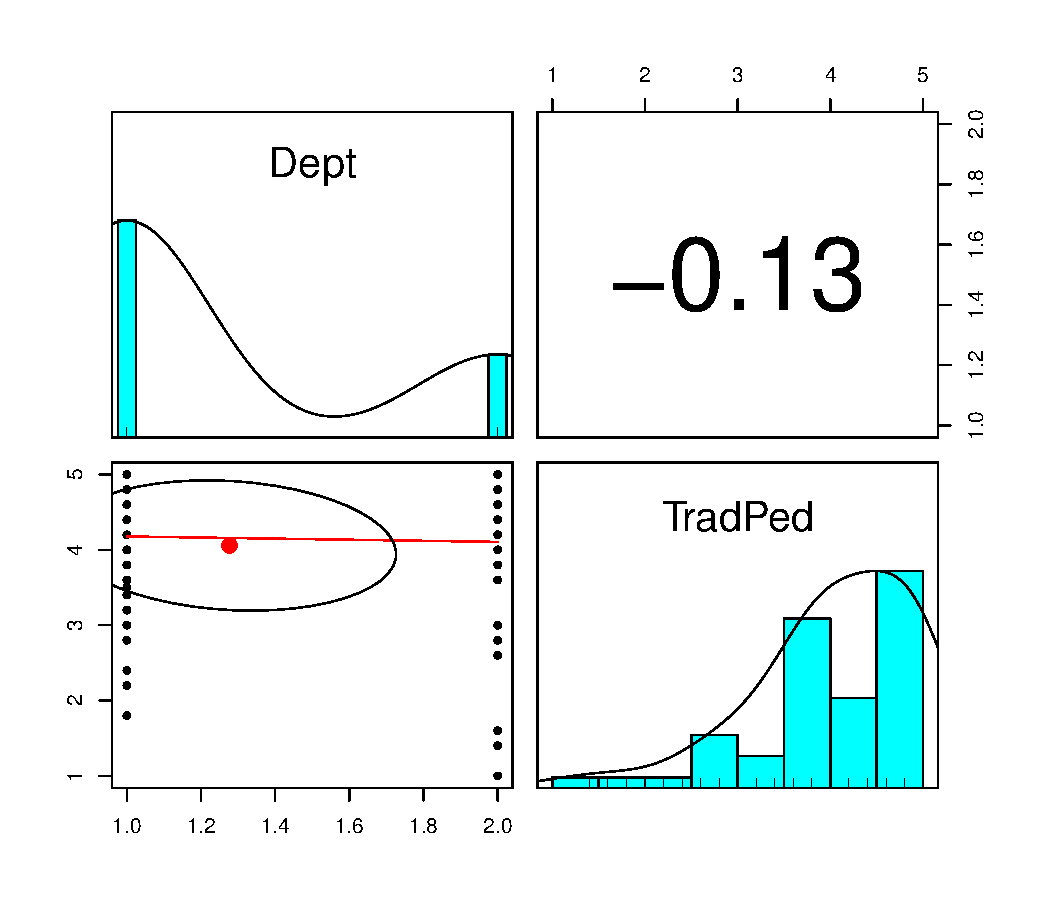
\includegraphics{05-tIndSample_files/figure-latex/unnamed-chunk-43-1.pdf}

We can see that we'll have more CPY students than ORG students. Although our kurtosis was below \textbar10\textbar{} our distribution looks negatively skewed, with the majority of the scores being on the high end of the scale.

And now for homogeneity of variance:

\begin{Shaded}
\begin{Highlighting}[]
\NormalTok{rstatix}\SpecialCharTok{::}\FunctionTok{levene\_test}\NormalTok{(IndT\_df, TradPed }\SpecialCharTok{\textasciitilde{}}\NormalTok{ Dept, }\AttributeTok{center =}\NormalTok{ median)}
\end{Highlighting}
\end{Shaded}

\begin{verbatim}
# A tibble: 1 x 4
    df1   df2 statistic     p
  <int> <int>     <dbl> <dbl>
1     1   110      2.46 0.120
\end{verbatim}

Levene's test for homogeneity of variance indicated that we did not violate the assumption of homogeneity of variance \((F[1, 110] = 2.460, p = 0.120)\). That is to say, the variance in each of the departments is not statistically significantly different from each other. We can use the regular (Student's) formulation of the \emph{t}-test for independent samples.

\hypertarget{conduct-an-independent-samples-t-test-with-an-effect-size-and-95cis}{%
\subsubsection{\texorpdfstring{Conduct an independent samples \emph{t}-test (with an effect size and 95\%CIs)}{Conduct an independent samples t-test (with an effect size and 95\%CIs)}}\label{conduct-an-independent-samples-t-test-with-an-effect-size-and-95cis}}

Conduct the independent samples \emph{t}-test (with an effect size)

\begin{Shaded}
\begin{Highlighting}[]
\NormalTok{indT.test }\OtherTok{\textless{}{-}}\NormalTok{ rstatix}\SpecialCharTok{::}\FunctionTok{t\_test}\NormalTok{(IndT\_df, TradPed }\SpecialCharTok{\textasciitilde{}}\NormalTok{ Dept, }\AttributeTok{var.equal =} \ConstantTok{TRUE}\NormalTok{,}
    \AttributeTok{detailed =} \ConstantTok{TRUE}\NormalTok{) }\SpecialCharTok{\%\textgreater{}\%}
\NormalTok{    rstatix}\SpecialCharTok{::}\FunctionTok{add\_significance}\NormalTok{()}
\NormalTok{indT.test}
\end{Highlighting}
\end{Shaded}

\begin{verbatim}
# A tibble: 1 x 16
  estimate estimate1 estimate2 .y.     group1 group2    n1    n2 statistic     p
     <dbl>     <dbl>     <dbl> <chr>   <chr>  <chr>  <int> <int>     <dbl> <dbl>
1    0.259      4.13      3.87 TradPed CPY    ORG       81    31      1.42 0.158
# i 6 more variables: df <dbl>, conf.low <dbl>, conf.high <dbl>, method <chr>,
#   alternative <chr>, p.signif <chr>
\end{verbatim}

From this output we learn that the value of the \emph{t}-test is 1.423 and is non-significant \emph{p = 0.148}. We are 95\% confident that the mean diference falls between -0.102 and 0.618. Because this thresshold crosses zero, we cannot be certain that the true difference in means is not zero. Here's how I would represent these results in a statistical string: \(t(110) = 1.423, p = 0.158, CI95 (0.102, 0.619)\).

Calculating the Cohen's \emph{d} as the effect size.

\begin{Shaded}
\begin{Highlighting}[]
\NormalTok{rstatix}\SpecialCharTok{::}\FunctionTok{cohens\_d}\NormalTok{(IndT\_df, TradPed }\SpecialCharTok{\textasciitilde{}}\NormalTok{ Dept, }\AttributeTok{var.equal =} \ConstantTok{TRUE}\NormalTok{)}
\end{Highlighting}
\end{Shaded}

\begin{verbatim}
# A tibble: 1 x 7
  .y.     group1 group2 effsize    n1    n2 magnitude
* <chr>   <chr>  <chr>    <dbl> <int> <int> <ord>    
1 TradPed CPY    ORG      0.300    81    31 small    
\end{verbatim}

The value of Cohen's \emph{d} statistic (interpreted in standard deviation units) is 0.300 and is small. We can add this value to the statistical string: \(t(110) = 1.423, p = 0.158, CI95 (0.102, 0.619), d = 0.300\).

\hypertarget{apa-style-results-with-tables-and-figure-1}{%
\subsubsection{APA style results with table(s) and figure}\label{apa-style-results-with-tables-and-figure-1}}

\begin{itemize}
\tightlist
\item
  Complete content of results (including t, df, p, d-or-eta, CI95\%)
\item
  Table
\item
  Figure
\item
  Grammar/formatting
\end{itemize}

\begin{quote}
An independent samples \emph{t}-test was conducted to evaluate the hypothesis that there would be differences in course evaluation ratings of traditional pedagogy between academic departments (CPY, ORG).
\end{quote}

\begin{quote}
We began by analyzing the data to see if it met the statistical assumptions for analysis with an independent samples \emph{t}-test. One assumption is that the dependent variable be normally distributed within the both levels of the grouping variable. We evaluated skew and kurtosis using Kline's \citeyearpar{kline_data_2016} guidelines of the absolute values of 3 (skew) and 10 (kurtosis). Our results were well-within these boundary conditions. Specifically, the traditional pedagogy ratings for CPY were -0.763 and 0.156 for skew and kurtosis, respectively; they were -1.183 and 0.583 for ORG. The Shapiro-Wilk test of normality indicated that the dependent variable, traditional pedagogy, differed significantly from a normal distribution for both CPY students \((W = 0.918, p < 0.001)\) and ORG students\((W = 0.851, p < 0.001)\). Levene's test for homogeneity of variance indicated that we did not violate the assumption of homogeneity of variance \((F[1, 110] = 2.460, p = 0.120)\). That is to say, the variance in each of the departments is not statistically significantly different from each other. Because the independent samples \emph{t}-test is relatively robust to violations of normality when samples sizes have at least 15 participants per cell \citep{green_using_2017} and there was no violation of the homogeneity of variance assumption we proceded with the Student's formulation of the \emph{t}-test for independent samples.
\end{quote}

\begin{quote}
The independent samples \emph{t}-test was nonsignificant, \(t(110) = 1.423, p = 0.158\), the effect size (d = 0.300) was small. The 95\% confidence interval for the difference in means ranged from -0.102 to 0.619. Means and standard deviations are presented in Table 1; the results are illustrated in Figure 1.
\end{quote}

We can use the \emph{apaTables} package to create a table of means and standard deviations.

\begin{Shaded}
\begin{Highlighting}[]
\NormalTok{apaTables}\SpecialCharTok{::}\FunctionTok{apa.1way.table}\NormalTok{(Dept, TradPed, IndT\_df)}
\end{Highlighting}
\end{Shaded}

\begin{verbatim}


Descriptive statistics for TradPed as a function of Dept.  

 Dept    M   SD
  CPY 4.13 0.75
  ORG 3.87 1.09

Note. M and SD represent mean and standard deviation, respectively.
 
\end{verbatim}

And now a figure.

\begin{Shaded}
\begin{Highlighting}[]
\NormalTok{indT.box }\OtherTok{\textless{}{-}}\NormalTok{ ggpubr}\SpecialCharTok{::}\FunctionTok{ggboxplot}\NormalTok{(IndT\_df, }\AttributeTok{x =} \StringTok{"Dept"}\NormalTok{, }\AttributeTok{y =} \StringTok{"TradPed"}\NormalTok{, }\AttributeTok{color =} \StringTok{"Dept"}\NormalTok{,}
    \AttributeTok{palette =} \FunctionTok{c}\NormalTok{(}\StringTok{"\#00AFBB"}\NormalTok{, }\StringTok{"\#FC4E07"}\NormalTok{), }\AttributeTok{add =} \StringTok{"jitter"}\NormalTok{, }\AttributeTok{title =} \StringTok{"Figure 1. Traditional Pedagogy as a Function of Academic Department"}\NormalTok{)}
\NormalTok{ind.testT }\OtherTok{\textless{}{-}}\NormalTok{ indT.test }\SpecialCharTok{\%\textgreater{}\%}
\NormalTok{    rstatix}\SpecialCharTok{::}\FunctionTok{add\_xy\_position}\NormalTok{(}\AttributeTok{x =} \StringTok{"Dept"}\NormalTok{)  }\CommentTok{\#autocomputes p{-}value labels positions}
\NormalTok{indT.box }\OtherTok{\textless{}{-}}\NormalTok{ indT.box }\SpecialCharTok{+}\NormalTok{ ggpubr}\SpecialCharTok{::}\FunctionTok{stat\_pvalue\_manual}\NormalTok{(ind.testT, }\AttributeTok{label =} \StringTok{"p.signif"}\NormalTok{,}
    \AttributeTok{tip.length =} \FloatTok{0.02}\NormalTok{, }\AttributeTok{hide.ns =} \ConstantTok{FALSE}\NormalTok{, }\AttributeTok{y.position =} \FunctionTok{c}\NormalTok{(}\DecValTok{6}\NormalTok{)) }\SpecialCharTok{+} \FunctionTok{labs}\NormalTok{(}\AttributeTok{subtitle =}\NormalTok{ rstatix}\SpecialCharTok{::}\FunctionTok{get\_test\_label}\NormalTok{(indT.test,}
    \AttributeTok{detailed =} \ConstantTok{TRUE}\NormalTok{))  }\CommentTok{\#adds t{-}test results}

\NormalTok{indT.box}
\end{Highlighting}
\end{Shaded}

\includegraphics{05-tIndSample_files/figure-latex/unnamed-chunk-48-1.pdf}

\hypertarget{conduct-power-analyses-to-determine-the-power-of-the-current-study-and-a-recommended-sample-size-1}{%
\subsubsection{Conduct power analyses to determine the power of the current study and a recommended sample size}\label{conduct-power-analyses-to-determine-the-power-of-the-current-study-and-a-recommended-sample-size-1}}

We can use Cohen's d in this specification of \emph{d}.

\begin{Shaded}
\begin{Highlighting}[]
\NormalTok{pwr}\SpecialCharTok{::}\FunctionTok{pwr.t.test}\NormalTok{(}\AttributeTok{d =} \FloatTok{0.30}\NormalTok{, }\AttributeTok{n =} \DecValTok{112}\NormalTok{, }\AttributeTok{power =} \ConstantTok{NULL}\NormalTok{, }\AttributeTok{sig.level =} \FloatTok{0.05}\NormalTok{,}
    \AttributeTok{type =} \StringTok{"two.sample"}\NormalTok{, }\AttributeTok{alternative =} \StringTok{"two.sided"}\NormalTok{)}
\end{Highlighting}
\end{Shaded}

\begin{verbatim}

     Two-sample t test power calculation 

              n = 112
              d = 0.3
      sig.level = 0.05
          power = 0.6084749
    alternative = two.sided

NOTE: n is number in *each* group
\end{verbatim}

We were at 61\% power. That is, given the value of the mean difference (), we had a 61\% chance of detecting a statistically significant effect if there was one. How big of a sample would it take?

\begin{Shaded}
\begin{Highlighting}[]
\NormalTok{pwr}\SpecialCharTok{::}\FunctionTok{pwr.t.test}\NormalTok{(}\AttributeTok{d =} \FloatTok{0.3}\NormalTok{, }\AttributeTok{n =} \ConstantTok{NULL}\NormalTok{, }\AttributeTok{power =} \FloatTok{0.8}\NormalTok{, }\AttributeTok{sig.level =} \FloatTok{0.05}\NormalTok{,}
    \AttributeTok{type =} \StringTok{"two.sample"}\NormalTok{, }\AttributeTok{alternative =} \StringTok{"two.sided"}\NormalTok{)}
\end{Highlighting}
\end{Shaded}

\begin{verbatim}

     Two-sample t test power calculation 

              n = 175.3847
              d = 0.3
      sig.level = 0.05
          power = 0.8
    alternative = two.sided

NOTE: n is number in *each* group
\end{verbatim}

To find a statistically significant difference, we would need 175 per group. This large size is consistent with the small effect -- that there isn't really a difference between the two groups..

\hypertarget{hand-calculations-2}{%
\subsection{Hand Calculations}\label{hand-calculations-2}}

\emph{Note: While the values of the hand-calculations are close to those calculated with the R packages, they differ slightly.}

\hypertarget{using-traditional-nhst-null-hypothesis-testing-language-state-your-null-and-alternative-hypotheses-1}{%
\subsubsection{Using traditional NHST (null hypothesis testing language), state your null and alternative hypotheses}\label{using-traditional-nhst-null-hypothesis-testing-language-state-your-null-and-alternative-hypotheses-1}}

\[H_0: \mu_1 = \mu_2\] \[H_A: \mu_1 \neq \mu_2\]

\hypertarget{using-an-r-package-or-functions-in-base-r-calculate-the-means-and-standard-deviations-for-both-levels-of-the-dependent-variable}{%
\subsubsection{Using an R package or functions in base R, calculate the means and standard deviations for both levels of the dependent variable}\label{using-an-r-package-or-functions-in-base-r-calculate-the-means-and-standard-deviations-for-both-levels-of-the-dependent-variable}}

\begin{Shaded}
\begin{Highlighting}[]
\NormalTok{psych}\SpecialCharTok{::}\FunctionTok{describeBy}\NormalTok{(IndT\_df }\SpecialCharTok{\textasciitilde{}}\NormalTok{ Dept, }\AttributeTok{type =}\DecValTok{1}\NormalTok{, }\AttributeTok{mat=}\ConstantTok{TRUE}\NormalTok{)}
\end{Highlighting}
\end{Shaded}

\begin{verbatim}
         item group1 vars  n     mean        sd median  trimmed     mad min max
Dept*1      1    CPY    1 81 1.000000 0.0000000    1.0 1.000000 0.00000 1.0   1
Dept*2      2    ORG    1 31 2.000000 0.0000000    2.0 2.000000 0.00000 2.0   2
TradPed1    3    CPY    2 81 4.129630 0.7547259    4.2 4.210769 0.88956 1.8   5
TradPed2    4    ORG    2 31 3.870968 1.0948953    4.0 4.040000 1.18608 1.0   5
         range       skew  kurtosis         se
Dept*1     0.0        NaN       NaN 0.00000000
Dept*2     0.0        NaN       NaN 0.00000000
TradPed1   3.2 -0.7630015 0.1555318 0.08385843
TradPed2   4.0 -1.1832786 0.5826528 0.19664900
\end{verbatim}

CPY: \emph{M} = 4.130, \emph{SD} = 0.755 ORG: \emph{M} = 3.871, \emph{SD} = 1.095

\hypertarget{calulate-the-se-used-in-the-denominator-of-the-t-test}{%
\subsubsection{\texorpdfstring{Calulate the SE used in the denominator of the \emph{t}-test}{Calulate the SE used in the denominator of the t-test}}\label{calulate-the-se-used-in-the-denominator-of-the-t-test}}

Just as a reminder, the SE is the denominator in the \emph{t}-test formula:

\[t = \frac{\bar{X_{1}} -\bar{X_{2}}}{\sqrt{\frac{s_{1}^{2}}{N_{1}}+\frac{s_{2}^{2}}{N_{2}}}}\]

\begin{Shaded}
\begin{Highlighting}[]
\FunctionTok{sqrt}\NormalTok{((}\FloatTok{0.7547259}\SpecialCharTok{\^{}}\DecValTok{2}\SpecialCharTok{/}\DecValTok{81}\NormalTok{) }\SpecialCharTok{+}\NormalTok{ (}\FloatTok{1.0948953}\SpecialCharTok{\^{}}\DecValTok{2}\SpecialCharTok{/}\DecValTok{31}\NormalTok{))}
\end{Highlighting}
\end{Shaded}

\begin{verbatim}
[1] 0.2137828
\end{verbatim}

The \emph{SE} = 0.214

\hypertarget{calculate-the-independent-samples-t-test}{%
\subsubsection{\texorpdfstring{Calculate the independent samples \emph{t}-test}{Calculate the independent samples t-test}}\label{calculate-the-independent-samples-t-test}}

\begin{Shaded}
\begin{Highlighting}[]
\NormalTok{(}\FloatTok{4.12963} \SpecialCharTok{{-}} \FloatTok{3.870968}\NormalTok{)}\SpecialCharTok{/}\FloatTok{0.2137828}
\end{Highlighting}
\end{Shaded}

\begin{verbatim}
[1] 1.209929
\end{verbatim}

\emph{I note that this hand calculation differs from the worked in R. I believe this is likely due to an unbalanced design with unequal cell sizes (81 and 31).}

\hypertarget{identify-the-degrees-of-freedom-associated-with-your-t-test-1}{%
\subsubsection{\texorpdfstring{Identify the degrees of freedom associated with your \emph{t}-test}{Identify the degrees of freedom associated with your t-test}}\label{identify-the-degrees-of-freedom-associated-with-your-t-test-1}}

\(N - 2\) is the degrees of freedom: 112-2, df = 110

\hypertarget{locate-the-test-critical-value-for-your-test-1}{%
\subsubsection{Locate the test critical value for your test}\label{locate-the-test-critical-value-for-your-test-1}}

We can look at a \href{https://www.statology.org/t-distribution-table/}{table of critical values}

For a two-tailed test, with alpha of 0.05, and a sample size of 120 (close enough), the \emph{t}-statistic must be greater than 1.98.

We could also obtain a \emph{t} critical value with this code:

\begin{Shaded}
\begin{Highlighting}[]
\FunctionTok{qt}\NormalTok{(}\FloatTok{0.05}\SpecialCharTok{/}\DecValTok{2}\NormalTok{, }\DecValTok{112}\NormalTok{, }\AttributeTok{lower.tail =} \ConstantTok{TRUE}\NormalTok{)}
\end{Highlighting}
\end{Shaded}

\begin{verbatim}
[1] -1.981372
\end{verbatim}

\begin{Shaded}
\begin{Highlighting}[]
\FunctionTok{qt}\NormalTok{(}\FloatTok{0.05}\SpecialCharTok{/}\DecValTok{2}\NormalTok{, }\DecValTok{112}\NormalTok{, }\AttributeTok{lower.tail =} \ConstantTok{FALSE}\NormalTok{)}
\end{Highlighting}
\end{Shaded}

\begin{verbatim}
[1] 1.981372
\end{verbatim}

\hypertarget{is-the-t-test-statistically-significant-why-or-why-not-1}{%
\subsubsection{\texorpdfstring{Is the \emph{t}-test statistically significant? Why or why not?}{Is the t-test statistically significant? Why or why not?}}\label{is-the-t-test-statistically-significant-why-or-why-not-1}}

In a two-tailed test, if the \emph{t}-statistic falls outside the boundaries of -1.98 and 1.98 the means of the two groups are statistically significantly different from each other.

My \emph{t} value of 1.209929 does not exceed these boundaries and therefore is not statistically significant.

\hypertarget{calculate-the-confidence-interval-around-the-difference-in-sample-means}{%
\subsubsection{Calculate the confidence interval around the difference in sample means}\label{calculate-the-confidence-interval-around-the-difference-in-sample-means}}

Calculating a confidence interval around the difference in sample means requires the two-tailed test critical values. We can insert them into this formula:

\[(\bar{X_{1}} -\bar{X_{2})} \pm  t_{cv}(SE)\]

\begin{Shaded}
\begin{Highlighting}[]
\NormalTok{(}\FloatTok{4.129630} \SpecialCharTok{{-}} \FloatTok{3.870968}\NormalTok{) }\SpecialCharTok{{-}}\NormalTok{ (}\FloatTok{1.209929} \SpecialCharTok{*} \FloatTok{0.2137828}\NormalTok{)}
\end{Highlighting}
\end{Shaded}

\begin{verbatim}
[1] -0.0000000094212
\end{verbatim}

\begin{Shaded}
\begin{Highlighting}[]
\NormalTok{(}\FloatTok{4.129630} \SpecialCharTok{{-}} \FloatTok{3.870968}\NormalTok{) }\SpecialCharTok{+}\NormalTok{ (}\FloatTok{1.209929} \SpecialCharTok{*} \FloatTok{0.2137828}\NormalTok{)}
\end{Highlighting}
\end{Shaded}

\begin{verbatim}
[1] 0.517324
\end{verbatim}

We are 95\% confident that the mean difference falls between -0.165 and 0.682. Because this interval passes through zero, we cannot be certain that the difference is 0. This is consistent with the non-significant \emph{p} value.

\hypertarget{calculate-the-effect-size-i.e.-cohens-d-associated-with-your-t-test-1}{%
\subsubsection{\texorpdfstring{Calculate the effect size (i.e., Cohen's d associated with your \emph{t}-test}{Calculate the effect size (i.e., Cohen's d associated with your t-test}}\label{calculate-the-effect-size-i.e.-cohens-d-associated-with-your-t-test-1}}

Here is the formula for Cohen's \emph{d}:

\[d = t\sqrt{\frac{N_{1}+N_{2}}{N_{1}N_{2}}}\]

\begin{Shaded}
\begin{Highlighting}[]
\FloatTok{1.209929} \SpecialCharTok{*}\NormalTok{ (}\FunctionTok{sqrt}\NormalTok{((}\DecValTok{81} \SpecialCharTok{+} \DecValTok{31}\NormalTok{)}\SpecialCharTok{/}\NormalTok{(}\DecValTok{81} \SpecialCharTok{*} \DecValTok{31}\NormalTok{)))}
\end{Highlighting}
\end{Shaded}

\begin{verbatim}
[1] 0.2555321
\end{verbatim}

\hypertarget{assemble-the-results-into-a-statistical-string}{%
\subsubsection{Assemble the results into a statistical string}\label{assemble-the-results-into-a-statistical-string}}

\(t(110) = 1.210, p > 0.05, CI95 (-0.000, 0.517), d = 0.256\)

\hypertarget{tPaired}{%
\chapter{\texorpdfstring{Paired Samples \emph{t}-test}{Paired Samples t-test}}\label{tPaired}}

\href{https://spu.hosted.panopto.com/Panopto/Pages/Viewer.aspx?pid=08a90f4e-ce0d-4a5f-93f1-af0101625dbc}{Screencasted Lecture Link}

Researchers are often interested in knowing if participants score differently on some outcome variable (like affective well-being) across two conditions. These conditions could be before and after an intervention; they could also be interventionless exposures such as scary versus funny movies. In these simple designs, the paired \emph{t}-test can be used to test the researchers' hypotheses.

\hypertarget{navigating-this-lesson-4}{%
\section{Navigating this Lesson}\label{navigating-this-lesson-4}}

There is about 45 minutes of lecture. If you work through the materials with me it would be plan for an additional hour

While the majority of R objects and data you will need are created within the R script that sources the chapter, occasionally there are some that cannot be created from within the R framework. Additionally, sometimes links fail. All original materials are provided at the \href{https://github.com/lhbikos/ReCenterPsychStats}{Github site} that hosts the book. More detailed guidelines for ways to access all these materials are provided in the OER's \protect\hyperlink{ReCintro}{introduction}

\hypertarget{learning-objectives-4}{%
\subsection{Learning Objectives}\label{learning-objectives-4}}

Learning objectives from this lecture include the following:

\begin{itemize}
\tightlist
\item
  Recognize the research questions for which utilization of paired sample \emph{t}-tests would be appropriate.
\item
  Narrate the steps in conducting a paired samples \emph{t}-test, beginning with testing the statistical assumptions through writing up an APA style results section.
\item
  Calculate a paired samples \emph{t}-test in R (including effect sizes).
\item
  Interpret a 95\% confidence interval around a mean difference score.
\item
  Produce an APA style results for a paired-samples \emph{t}-test.
\item
  Determine a sample size that (given a set of parameters) would likely result in a statistically significant effect, if there was one.
\end{itemize}

\hypertarget{planning-for-practice-3}{%
\subsection{Planning for Practice}\label{planning-for-practice-3}}

The suggestions for homework vary in degree of complexity. The more complete descriptions at the end of the chapter follow these suggestions.

\begin{itemize}
\tightlist
\item
  Rework the paired samples \emph{t}-test in the lesson by changing the random seed in the code that simulates the data. This should provide minor changes to the data, but the results will likely be very similar.
\item
  Rework the paired samples \emph{t}-test in the lesson by changing something else about the simulation. For example, if you are interested in power, consider changing the sample size.
\item
  Use the simulated data that is provided, but use the nonverbal variable, instead.
\item
  Conduct paired \emph{t}-test with data to which you have access and permission to use. This could include data you simulate on your own or from a published article.
\end{itemize}

\hypertarget{readings-resources-3}{%
\subsection{Readings \& Resources}\label{readings-resources-3}}

In preparing this chapter, I drew heavily from the following resource(s). Other resources are cited (when possible, linked) in the text with complete citations in the reference list.

\begin{itemize}
\tightlist
\item
  How to Do Paired T-test in R: The Best Tutorial You Will Love. (n.d.). Datanovia. Retrieved May 25, 2023, from \url{https://www.datanovia.com/en/lessons/how-to-do-a-t-test-in-r-calculation-and-reporting/how-to-do-paired-t-test-in-r/}

  \begin{itemize}
  \tightlist
  \item
    This tutorial provides a demonstration of the paired sampes t-test using the \emph{rstatix} package.
  \end{itemize}
\item
  Navarro, D. (2020). Chapter 13: Comparing two means. In \href{https://learningstatisticswithr.com/}{Learning Statistics with R - A tutorial for Psychology Students and other Beginners}. Retrieved from \url{https://stats.libretexts.org/Bookshelves/Applied_Statistics/Book\%3A_Learning_Statistics_with_R_-_A_tutorial_for_Psychology_Students_and_other_Beginners_(Navarro)}

  \begin{itemize}
  \tightlist
  \item
    Navarro's OER includes a good mix of conceptual information about \emph{t}-tests as well as R code. My lesson integrates her approach as well as considering information from Field's \citeyearpar{field_discovering_2012} and Green and Salkind's \citep{green_using_2017} texts (as well as searching around on the internet).
  \end{itemize}
\item
  Elliott, A. M., Alexander, S. C., Mescher, C. A., Mohan, D., \& Barnato, A. E. (2016). Differences in Physicians' Verbal and Nonverbal Communication With Black and White Patients at the End of Life. \emph{Journal of Pain and Symptom Management, 51}(1), 1--8. \url{https://doi.org/10.1016/j.jpainsymman.2015.07.008}

  \begin{itemize}
  \tightlist
  \item
    The source of our research vignette.
  \end{itemize}
\end{itemize}

\hypertarget{packages-2}{%
\subsection{Packages}\label{packages-2}}

The script below will (a) check to see if the following packages are installed on your computer and, if not (b) install them.

\begin{Shaded}
\begin{Highlighting}[]
\CommentTok{\# will install the package if not already installed}
\CommentTok{\# if(!require(psych))\{install.packages(\textquotesingle{}psych\textquotesingle{})\}}
\CommentTok{\# if(!require(faux))\{install.packages(\textquotesingle{}faux\textquotesingle{})\}}
\CommentTok{\# if(!require(tidyverse))\{install.packages(\textquotesingle{}tidyverse\textquotesingle{})\}}
\CommentTok{\# if(!require(dplyr))\{install.packages(\textquotesingle{}dplyr\textquotesingle{})\}}
\CommentTok{\# if(!require(ggpubr))\{install.packages(\textquotesingle{}ggpubr\textquotesingle{})\}}
\CommentTok{\# if(!require(pwr))\{install.packages(\textquotesingle{}pwr\textquotesingle{})\}}
\CommentTok{\# if(!require(apaTables))\{install.packages(\textquotesingle{}apaTables\textquotesingle{})\}}
\CommentTok{\# if(!require(knitr))\{install.packages(\textquotesingle{}knitr\textquotesingle{})\}}
\CommentTok{\# if(!require(rstatix))\{install.packages(\textquotesingle{}rstatix\textquotesingle{})\}}
\end{Highlighting}
\end{Shaded}

\hypertarget{introducing-the-paired-samples-t-test}{%
\section{\texorpdfstring{Introducing the Paired Samples \emph{t}-test}{Introducing the Paired Samples t-test}}\label{introducing-the-paired-samples-t-test}}

There are a couple of typical use cases for the paired samples \emph{t}-test. Repeated measures or change-over-time is a very common use. In this case, the research participant may take a pre-test, be exposed to an intervention or other type of stimulus, then take a post-test. Owing to the limitations of the statistics, all participants must be exposed to the same intervention/stimulus.

\begin{figure}
\centering
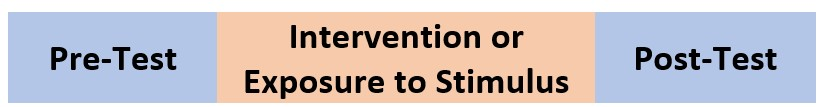
\includegraphics{images/ttests/prepost_paired.jpg}
\caption{An image of a row with three boxes: pre-test (in blue), intervention or exposure to stimulus (in light red), post-test (in blue) representing the use of a paired samples \emph{t}-test in a repeated measures design}
\end{figure}

A second common use is the assessment of a research participant in two competing conditions. An example might be the galvanic skin response ratings when a participant's hand is submerged in ice versus the GSR ratings when the hand is not exposed in ice. A strength of this design is the within-subjects' control of the participant.

\begin{figure}
\centering

\includegraphics{images/ttests/conditions_paired.jpg}
\caption{An image of a row with two boxes labeled Condition A in light blue) and Condition B (in dark blue). This represents the use of a paired samples \emph{t}-test to compare across conditions}
\end{figure}

In the formula for the paired samples \emph{t}-test we see a \(\bar{D}\) in the numerator. This represents the \emph{difference} between the continuously scaled scores in the two conditions. The denominator involves a standard deviation of the difference scores (\(\hat\sigma_D\)) and the square root of the sample size.

\[t = \frac{\bar{D}}{\hat\sigma_D / \sqrt{N}}\] Although these types of research design and analyses are quite handy, they have some limitations. First, the paired samples \emph{t}-test cannot establish causality because it lacks elements such as comparing conditions (e.g., treatment vs.~control) and random assignment to those conditions. If a research wants to compare pre-post change as a result of participating in more-than-one condition, a \protect\hyperlink{Mixed}{mixed design ANOVA} would be a better option. Second, the paired samples \emph{t}-test cannot accommodate more than two comparison conditions. If the researcher wants to compare three or or more time periods or conditions, they will want to consider \protect\hyperlink{Repeated}{repeated measures ANOVA} or \href{https://lhbikos.github.io/MultilevelModeling/}{multilevel/hierarchical linear modeling}.

\hypertarget{workflow-for-paired-samples-t-test}{%
\subsection{\texorpdfstring{Workflow for Paired Samples \emph{t}-test}{Workflow for Paired Samples t-test}}\label{workflow-for-paired-samples-t-test}}

The following is a proposed workflow for conducting the paired samples \emph{t}-test.

\begin{figure}
\centering
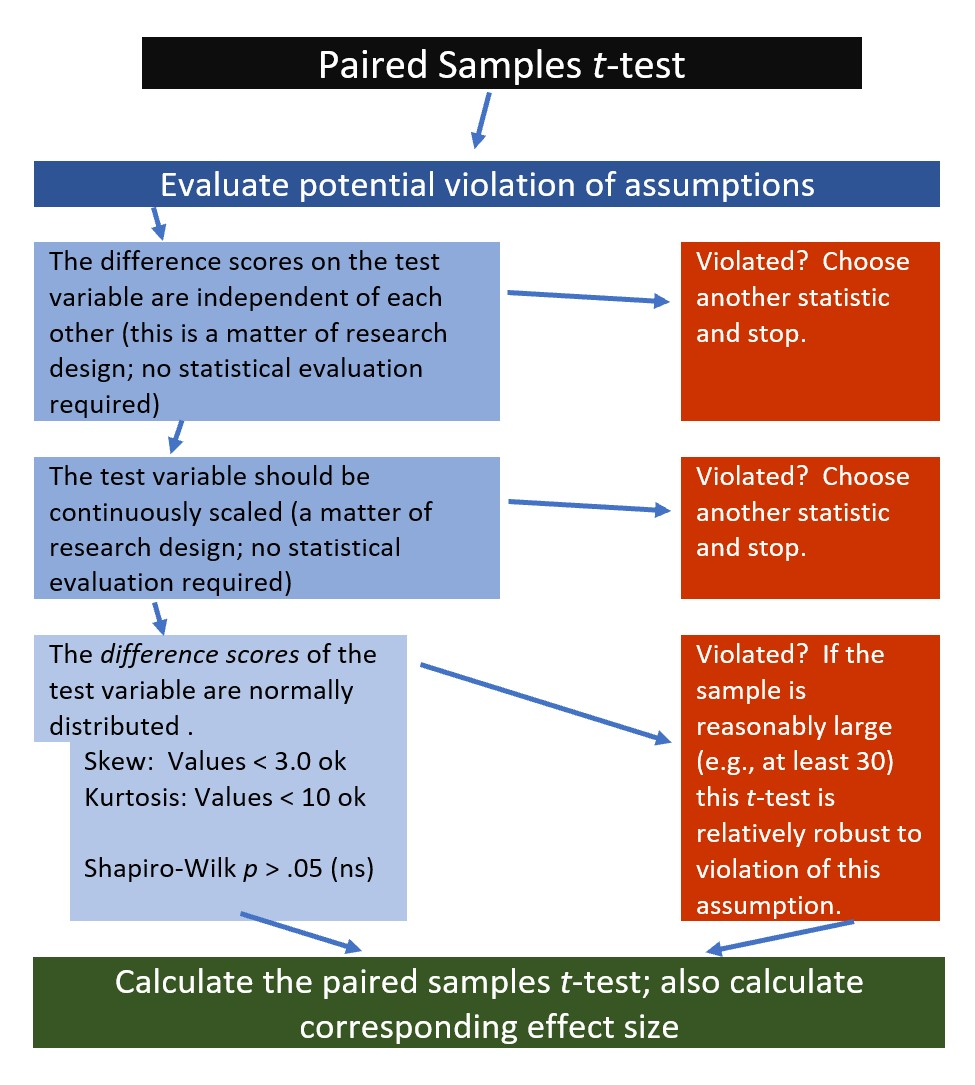
\includegraphics{images/ttests/PairedSampleWrkFlw.jpg}
\caption{A colorful image of a workflow for the paired samples \emph{t}-test}
\end{figure}

If the data meets the assumptions associated with the research design (e.g., independence of difference scores and a continuously scaled metric for that difference score), these are the steps for the analysis of an independent samples \emph{t}-test:

\begin{enumerate}
\def\labelenumi{\arabic{enumi}.}
\tightlist
\item
  Prepare (upload) data.
\item
  Explore data with

  \begin{itemize}
  \tightlist
  \item
    graphs
  \item
    descriptive statistics
  \end{itemize}
\item
  Assess normality of the difference scores via skew and kurtosis
\item
  Compute the paired samples \emph{t}-test
\item
  Compute an effect size (frequently the \emph{d} or \emph{eta} statistic)
\item
  Manage Type I error
\item
  Sample size/power analysis (which you should think about first, but in the context of teaching statistics, it's more pedagogically sensible, here).
\end{enumerate}

\hypertarget{research-vignette-3}{%
\section{Research Vignette}\label{research-vignette-3}}

Empirically published articles where \emph{t}-tests are the primary statistic are difficult to locate. Having exhausted the psychology archives, I located this article in an interdisciplinary journal focused on palliative medicine. The research vignette for this lesson examined differences in physician's verbal and nonverbal communication with Black and White patients at the end of life \citep{elliott_differences_2016}.

Elliott and colleagues \citeyearpar{elliott_differences_2016} were curious to know if hospital-based physicians (56\% White, 26\% Asian, 7.4\% each Black and Hispanic) engaged in verbal and nonverbal communication differently with Black and White patients. Black and White patient participants were matched on characteristics deemed important to the researchers (e.g., critically and terminally ill, prognostically similar). Interactions in the intensive care unit were audio and video recorded and then coded on dimensions of verbal and nonverbal communication.

Because each physician saw a pair of patients (i.e., one Black patient and one White patient), the researchers utilized a paired samples, or dependent \emph{t}-test. This statistical choice was consistent with the element of the research design that controlled for physician effects through matching patients on critical characteristics. Below are the primary findings of the study.

\begin{longtable}[]{@{}llll@{}}
\toprule\noalign{}
& Black Patients & White Patients & \\
\midrule\noalign{}
\endhead
\bottomrule\noalign{}
\endlastfoot
Category & \emph{Mean}(\emph{SD}) & \emph{Mean}(\emph{SD}) & \emph{p}-value \\
Verbal skill score (range 0 - 27) & 8.37(3.36) & 8.41(3.21) & 0.958 \\
Nonverbal skill score (range 0 - 5) & 2.68(.84) & 2.93(.77) & 0.014 \\
\end{longtable}

The primary analysis utilized by Elliott and colleagues \citeyearpar{elliott_differences_2016} was the paired samples \emph{t}-test. We will replicate that exact analysis with simulated data.

\hypertarget{simulating-data-for-the-paired-samples-t-test}{%
\subsection{\texorpdfstring{Simulating Data for the Paired Samples \emph{t}-test}{Simulating Data for the Paired Samples t-test}}\label{simulating-data-for-the-paired-samples-t-test}}

Below is the code I used to simulate the data. The following code assumes 33 physician participants who had separate interactions with critically ill, end-of-life stage patients, who were identified as Black and White. The Elliott et al. \citeyearpar{elliott_differences_2016} manuscript describe the process for coding verbal and nonverbal communication for video/audio recordings of the physician/patient interactions. Using that data, I simulate verbal and nonverbal communication scores for 33 physicians who rate patients who identify as Black and White, respectively. This creates four variables.

In the lesson, we will compare verbal communication scores. The nonverbal communication score is available as an option for practice.

\begin{Shaded}
\begin{Highlighting}[]
\FunctionTok{library}\NormalTok{(tidyverse)}
\end{Highlighting}
\end{Shaded}

\begin{verbatim}
-- Attaching core tidyverse packages ------------------------ tidyverse 2.0.0 --
v dplyr     1.1.2     v readr     2.1.4
v forcats   1.0.0     v stringr   1.5.0
v ggplot2   3.4.2     v tibble    3.2.1
v lubridate 1.9.2     v tidyr     1.3.0
v purrr     1.0.1     
-- Conflicts ------------------------------------------ tidyverse_conflicts() --
x dplyr::filter() masks stats::filter()
x dplyr::lag()    masks stats::lag()
i Use the conflicted package (<http://conflicted.r-lib.org/>) to force all conflicts to become errors
\end{verbatim}

\begin{Shaded}
\begin{Highlighting}[]
\CommentTok{\# Setting the seed. If you choose this practice option, change the}
\CommentTok{\# number below to something different.}
\FunctionTok{set.seed}\NormalTok{(}\DecValTok{220817}\NormalTok{)}
\CommentTok{\# These define the characteristics of the verbal variable. It is}
\CommentTok{\# essential that the object names (e.g., A\_mean) are not changed}
\CommentTok{\# because they will be fed to the function in the faux package.}
\NormalTok{sub\_n }\OtherTok{\textless{}{-}} \DecValTok{33}
\NormalTok{A\_mean }\OtherTok{\textless{}{-}} \FloatTok{8.37}
\NormalTok{B\_mean }\OtherTok{\textless{}{-}} \FloatTok{8.41}
\NormalTok{A\_sd }\OtherTok{\textless{}{-}} \FloatTok{3.36}
\NormalTok{B\_sd }\OtherTok{\textless{}{-}} \FloatTok{3.21}
\NormalTok{AB\_r }\OtherTok{\textless{}{-}} \FloatTok{0.3}

\CommentTok{\# the faux package can simulate a variety of data. This function}
\CommentTok{\# within the faux package will use the objects above to simulate}
\CommentTok{\# paired samples data}
\NormalTok{paired\_V }\OtherTok{\textless{}{-}}\NormalTok{ faux}\SpecialCharTok{::}\FunctionTok{rnorm\_multi}\NormalTok{(}\AttributeTok{n =}\NormalTok{ sub\_n, }\AttributeTok{vars =} \DecValTok{2}\NormalTok{, }\AttributeTok{r =}\NormalTok{ AB\_r, }\AttributeTok{mu =} \FunctionTok{c}\NormalTok{(A\_mean,}
\NormalTok{    B\_mean), }\AttributeTok{sd =} \FunctionTok{c}\NormalTok{(A\_sd, B\_sd), }\AttributeTok{varnames =} \FunctionTok{c}\NormalTok{(}\StringTok{"Verbal\_BL"}\NormalTok{, }\StringTok{"Verbal\_WH"}\NormalTok{))}

\NormalTok{paired\_V }\OtherTok{\textless{}{-}}\NormalTok{ paired\_V }\SpecialCharTok{\%\textgreater{}\%}
\NormalTok{    dplyr}\SpecialCharTok{::}\FunctionTok{mutate}\NormalTok{(}\AttributeTok{PhysID =} \FunctionTok{row\_number}\NormalTok{())}

\CommentTok{\# Here, I repeated the process for the nonverbal variable.}
\NormalTok{sub\_n }\OtherTok{\textless{}{-}} \DecValTok{33}
\NormalTok{A\_mean }\OtherTok{\textless{}{-}} \FloatTok{2.68}
\NormalTok{B\_mean }\OtherTok{\textless{}{-}} \FloatTok{2.93}
\NormalTok{A\_sd }\OtherTok{\textless{}{-}} \FloatTok{0.84}
\NormalTok{B\_sd }\OtherTok{\textless{}{-}} \FloatTok{0.77}
\NormalTok{AB\_r }\OtherTok{\textless{}{-}} \FloatTok{0.9}

\NormalTok{paired\_NV }\OtherTok{\textless{}{-}}\NormalTok{ faux}\SpecialCharTok{::}\FunctionTok{rnorm\_multi}\NormalTok{(}\AttributeTok{n =}\NormalTok{ sub\_n, }\AttributeTok{vars =} \DecValTok{2}\NormalTok{, }\AttributeTok{r =}\NormalTok{ AB\_r, }\AttributeTok{mu =} \FunctionTok{c}\NormalTok{(A\_mean,}
\NormalTok{    B\_mean), }\AttributeTok{sd =} \FunctionTok{c}\NormalTok{(A\_sd, B\_sd), }\AttributeTok{varnames =} \FunctionTok{c}\NormalTok{(}\StringTok{"NVerb\_BL"}\NormalTok{, }\StringTok{"NVerb\_WH"}\NormalTok{))}

\CommentTok{\# This code produced an ID number for each physician}
\NormalTok{paired\_NV }\OtherTok{\textless{}{-}}\NormalTok{ paired\_NV }\SpecialCharTok{\%\textgreater{}\%}
\NormalTok{    dplyr}\SpecialCharTok{::}\FunctionTok{mutate}\NormalTok{(}\AttributeTok{PhysID =} \FunctionTok{row\_number}\NormalTok{())}

\CommentTok{\# This data joined the two sets of data.  Note, I did not write any}
\CommentTok{\# code that assumed tha the verbal and nonverbal data came from the}
\CommentTok{\# same physician.  Full confession: I\textquotesingle{}m not quite sure how to do that}
\CommentTok{\# just yet.}
\NormalTok{dfPairedSamples }\OtherTok{\textless{}{-}}\NormalTok{ dplyr}\SpecialCharTok{::}\FunctionTok{full\_join}\NormalTok{(paired\_V, paired\_NV, }\AttributeTok{by =} \FunctionTok{c}\NormalTok{(}\StringTok{"PhysID"}\NormalTok{))}
\NormalTok{dfPairedSamples }\OtherTok{\textless{}{-}}\NormalTok{ dfPairedSamples }\SpecialCharTok{\%\textgreater{}\%}
\NormalTok{    dplyr}\SpecialCharTok{::}\FunctionTok{select}\NormalTok{(PhysID, }\FunctionTok{everything}\NormalTok{())}
\end{Highlighting}
\end{Shaded}

Before beginning our analysis, let's check the format of the variables to see if they are consistent with the scale of measurement of the variables. In our case, we expect to see four variables representing the verbal and nonverbal communication of the physicians with the patients who are identified as Black and White. Each of the variables should be continuously scaled and, therefore, should be formatted as \emph{num} (numerical).

\begin{Shaded}
\begin{Highlighting}[]
\FunctionTok{str}\NormalTok{(dfPairedSamples)}
\end{Highlighting}
\end{Shaded}

\begin{verbatim}
'data.frame':   33 obs. of  5 variables:
 $ PhysID   : int  1 2 3 4 5 6 7 8 9 10 ...
 $ Verbal_BL: num  8.19 3.3 6.18 4.85 6.91 ...
 $ Verbal_WH: num  4.63 12.85 13.47 6.49 12.27 ...
 $ NVerb_BL : num  3.099 4.234 0.429 1.835 3.704 ...
 $ NVerb_WH : num  2.74 5.02 1.34 2.38 2.91 ...
\end{verbatim}

The four variables of interest are correctly formatted as \emph{num}. Because PhysID (physician ID) will not be used in our analysis, its structure is irrelevant.

Below is code for saving (and then importing) the data in .csv or .rds files. I make choices about saving data based on what I wish to do with the data. If I want to manipulate the data outside of R, I will save it as a .csv file. It is easy to open .csv files in Excel. A limitation of the .csv format is that it does not save any restructuring or reformatting of variables. For this lesson, this is not an issue.

Here is code for saving the data as a .csv and then reading it back into R. I have hashtagged these out, so you will need to remove the hashtags if you wish to run any of these operations.

\begin{Shaded}
\begin{Highlighting}[]
\CommentTok{\# writing the simulated data as a .csv write.table(dfPairedSamples,}
\CommentTok{\# file = \textquotesingle{}dfPairedSamples.csv\textquotesingle{}, sep = \textquotesingle{},\textquotesingle{}, col.names=TRUE,}
\CommentTok{\# row.names=FALSE) at this point you could clear your environment and}
\CommentTok{\# then bring the data back in as a .csv reading the data back in as a}
\CommentTok{\# .csv file dfPairedSamples\textless{}{-} read.csv (\textquotesingle{}dfPairedSamples.csv\textquotesingle{}, header}
\CommentTok{\# = TRUE)}
\end{Highlighting}
\end{Shaded}

The .rds form of saving variables preserves any formatting (e.g., creating ordered factors) of the data. A limitation is that these files are not easily opened in Excel. Here is the hashtagged code (remove hashtags if you wish to do this) for writing (and then reading) this data as an .rds file.

\begin{Shaded}
\begin{Highlighting}[]
\CommentTok{\# saveRDS(dfPairedSamples, \textquotesingle{}dfPairedSamples.rds\textquotesingle{}) dfPairedSamples \textless{}{-}}
\CommentTok{\# readRDS(\textquotesingle{}dfPairedSamples.rds\textquotesingle{})}
\end{Highlighting}
\end{Shaded}

\hypertarget{quick-peek-at-the-data-2}{%
\subsection{Quick Peek at the Data}\label{quick-peek-at-the-data-2}}

Plotting the data is a helpful early step in any data analysis. Further, visualizing the data can help us with a conceptual notion of the statistic we are utilizing. The \emph{ggpubr} package is one of my go-to-tools for quick and easy plots of data. The \emph{ggpaired()} function is especially appropriate for paired data. A \href{https://rpkgs.datanovia.com/ggpubr/reference/ggpaired.html}{tutorial} is available at datanovia.

Especially unique about this function is that the lines connect the scores of each person across time or conditions. In this research scenario, the lines present the amount of time the physicians spent with each of the two patients they treated.

\begin{Shaded}
\begin{Highlighting}[]
\NormalTok{ggpubr}\SpecialCharTok{::}\FunctionTok{ggpaired}\NormalTok{(dfPairedSamples, }\AttributeTok{cond1 =} \StringTok{"Verbal\_BL"}\NormalTok{, }\AttributeTok{cond2 =} \StringTok{"Verbal\_WH"}\NormalTok{,}
    \AttributeTok{color =} \StringTok{"condition"}\NormalTok{, }\AttributeTok{line.color =} \StringTok{"gray"}\NormalTok{, }\AttributeTok{palette =} \FunctionTok{c}\NormalTok{(}\StringTok{"npg"}\NormalTok{), }\AttributeTok{xlab =} \StringTok{"Patient Race"}\NormalTok{,}
    \AttributeTok{ylab =} \StringTok{"Verbal Communication Rating"}\NormalTok{)}
\end{Highlighting}
\end{Shaded}

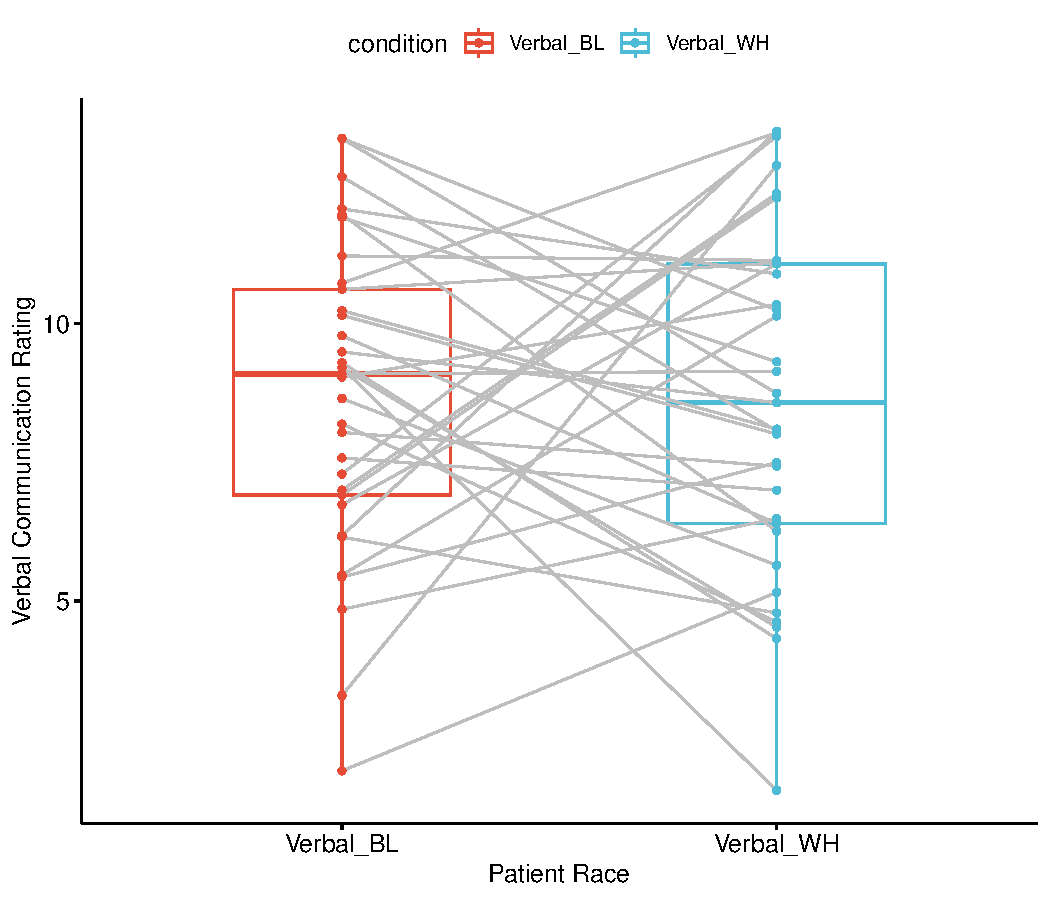
\includegraphics{06-tPairedSamples_files/figure-latex/unnamed-chunk-7-1.pdf} The box of the boxplot covers the middle 50\% (the interquartile range). The horizontal line is the median. The whiskers represent three standard deviations above and below the mean. Any dots beyond the whiskers are outliers.

\hypertarget{working-the-paired-samples-t-test-by-hand}{%
\section{\texorpdfstring{Working the Paired Samples \emph{t}-Test (by hand)}{Working the Paired Samples t-Test (by hand)}}\label{working-the-paired-samples-t-test-by-hand}}

\hypertarget{stating-the-hypothesis-2}{%
\subsection{Stating the Hypothesis}\label{stating-the-hypothesis-2}}

In this lesson, I will focus on differences in the verbal communication variable. Specifically, I hypothesize that physician verbal communication scores for Black and White patients will differ. In the hypotheses below, the null hypothesis (\(\mu_D\)) states that the difference score is zero; the alternative hypothesis (\(\mu_D\)) states that the difference score is different from zero.

\[H_{O}: \mu _{D} = 0\] \[H_{A}: \mu _{D} \neq 0\]

Notice the focus on a \emph{difference} score. Even though the R package we will use does not require one for calculation, creating one in our df will be useful for preliminary exploration.

\begin{Shaded}
\begin{Highlighting}[]
\CommentTok{\# Creating the Verbal\_D variable within the dfPairedSamples df Doing}
\CommentTok{\# the \textquotesingle{}math\textquotesingle{} that informs that variable}
\NormalTok{dfPairedSamples}\SpecialCharTok{$}\NormalTok{Verbal\_D }\OtherTok{\textless{}{-}}\NormalTok{ (dfPairedSamples}\SpecialCharTok{$}\NormalTok{Verbal\_BL }\SpecialCharTok{{-}}\NormalTok{ dfPairedSamples}\SpecialCharTok{$}\NormalTok{Verbal\_WH)}
\CommentTok{\# Displaying the first six rows of the df to show that the difference}
\CommentTok{\# score now exists}
\FunctionTok{head}\NormalTok{(dfPairedSamples)}
\end{Highlighting}
\end{Shaded}

\begin{verbatim}
  PhysID Verbal_BL Verbal_WH  NVerb_BL NVerb_WH  Verbal_D
1      1  8.190342  4.625680 3.0991101 2.742055  3.564663
2      2  3.297486 12.851362 4.2338398 5.024047 -9.553876
3      3  6.176386 13.466880 0.4288566 1.337259 -7.290495
4      4  4.851426  6.488762 1.8347393 2.379431 -1.637336
5      5  6.911155 12.266646 3.7035910 2.914445 -5.355491
6      6 11.965831  6.259292 1.5369696 1.598493  5.706540
\end{verbatim}

Examining this new variable, because we subtracted the verbal communication ratings of physicians with White patients from those of Black patients a negative score means that physicians had lower verbal engagement with Black patients; a positive score means that physicians had more verbal engagement with White patients.

\hypertarget{calculating-the-paired-samples-t-test}{%
\subsection{\texorpdfstring{Calculating the Paired Samples \emph{t}-Test}{Calculating the Paired Samples t-Test}}\label{calculating-the-paired-samples-t-test}}

Let's take another look at the formula for calculating paired samples \emph{t}-test.

\[t = \frac{\bar{D}}{\hat\sigma_D / \sqrt{N}}\] We can use the data from our preliminary exploration in the calculation.

\begin{itemize}
\tightlist
\item
  The mean difference was .08
\item
  The standard deviation of that difference was 4.14
\item
  The sample size is 33
\end{itemize}

\begin{Shaded}
\begin{Highlighting}[]
\FloatTok{0.08}\SpecialCharTok{/}\NormalTok{(}\FloatTok{4.14}\SpecialCharTok{/}\FunctionTok{sqrt}\NormalTok{(}\DecValTok{33}\NormalTok{))}
\end{Highlighting}
\end{Shaded}

\begin{verbatim}
[1] 0.111006
\end{verbatim}

The resultant \emph{t} value is 0.111

Hopefully, this hand-calculation provided an indication of how the means, standard deviation, and sample sizes contribute to the estimate of this \emph{t}-test value. Now we ask, ``But it is statistically significant?''

\hypertarget{statistical-significance-2}{%
\subsubsection{Statistical Significance}\label{statistical-significance-2}}

Our \emph{t}-value was 0.111. We compare this value to the test critical value in a table of \emph{t} critical values. In-so-doing we must know our degrees of freedom. Because the numerator in a paired samples \emph{t}-test is a single difference score \(\bar{D}\), the associated degrees of freedom is \(N-1\). We must also specify the \emph{p} value (in our case .05) and whether-or-not our hypothesis is unidirectional or bi-directional. Our question only asked, ``Are the verbal communication levels different?'' In this case, the test is two-tailed, or bi-directional.

Let's return to the \href{https://www.statology.org/t-distribution-table/}{table of critical values} for the \emph{t} distribution to compare our \emph{t}-value (0.111) to the column that is appropriate for our:

\begin{itemize}
\tightlist
\item
  Degrees of freedom (in this case \(N-1\) or 32)
\item
  Alpha, as represented by \(p < .05\)
\item
  Specification as a one-tailed or two-tailed test

  \begin{itemize}
  \tightlist
  \item
    Our alternative hypothesis made no prediction about the direction of the difference; therefore we will use a two-tailed test
  \end{itemize}
\end{itemize}

In the linked table, when the degrees of freedom reaches 30, there larger intervals. We will use the row representing degrees of freedom of 30. If our \emph{t}-test value is lower than an absolute value of -2.042 or greater than the absolute value of 2.042, then our means are statistically significantly different from each other. In our case, we have not achieved statistical significance and we cannot say that the means are different. The \emph{t} string would look like this: \(t(32) = 0.111, p > .05\)

We can also use the \emph{qt()} function in base R. In the script below, I have indicated an alpha of .05. The ``2'' that follows indicates I want a two-tailed test. The 32 represents my degrees of freedom (\(N-1\)). In a two-tailed test, the regions of rejection will be below the lowerbound (lower.tail=TRUE) and above the upperbound (lower.tail=FALSE).

\begin{Shaded}
\begin{Highlighting}[]
\FunctionTok{qt}\NormalTok{(}\FloatTok{0.05}\SpecialCharTok{/}\DecValTok{2}\NormalTok{, }\DecValTok{32}\NormalTok{, }\AttributeTok{lower.tail =} \ConstantTok{TRUE}\NormalTok{)}
\end{Highlighting}
\end{Shaded}

\begin{verbatim}
[1] -2.036933
\end{verbatim}

\begin{Shaded}
\begin{Highlighting}[]
\FunctionTok{qt}\NormalTok{(}\FloatTok{0.05}\SpecialCharTok{/}\DecValTok{2}\NormalTok{, }\DecValTok{32}\NormalTok{, }\AttributeTok{lower.tail =} \ConstantTok{FALSE}\NormalTok{)}
\end{Highlighting}
\end{Shaded}

\begin{verbatim}
[1] 2.036933
\end{verbatim}

If our \emph{t} value is below the lowerbound (-2.04) or above the upper bound (2.04), then we have rejected the null hypothesis in favor of the alternative. As we demonstrated in the hand-calculations, we have not. The ratings of physicians' verbal engagement with patients who are racially identified as Black and White are not statistically significant.

\hypertarget{confidence-intervals-2}{%
\subsubsection{Confidence Intervals}\label{confidence-intervals-2}}

How confident are we in our result? With paired samples \emph{t}-tests, it is common to report an interval in which we are 95\% confident that our true mean difference exists. Below is the formula, which involves:

\begin{itemize}
\tightlist
\item
  \(\bar{D}\) the mean difference score
\item
  \(t_{cv}\) the test critical value for a two-tailed model (even if the hypothesis was one-tailed) where \(\alpha = .05\) and the degrees of freedom are \(N-1\)
\item
  \(s_{d}\) the standard deviation of \(\bar{D}\)
\item
  \(N\) sample size
\end{itemize}

\[\bar{D}\pm t_{cv}(s_{d}/\sqrt{n})\] Let's calculate it:

First, let's get the proper \emph{t} critical value:

\begin{Shaded}
\begin{Highlighting}[]
\FunctionTok{qt}\NormalTok{(}\FloatTok{0.05}\SpecialCharTok{/}\DecValTok{2}\NormalTok{, }\DecValTok{32}\NormalTok{, }\AttributeTok{lower.tail =} \ConstantTok{TRUE}\NormalTok{)}
\end{Highlighting}
\end{Shaded}

\begin{verbatim}
[1] -2.036933
\end{verbatim}

\begin{Shaded}
\begin{Highlighting}[]
\FunctionTok{qt}\NormalTok{(}\FloatTok{0.05}\SpecialCharTok{/}\DecValTok{2}\NormalTok{, }\DecValTok{32}\NormalTok{, }\AttributeTok{lower.tail =} \ConstantTok{FALSE}\NormalTok{)}
\end{Highlighting}
\end{Shaded}

\begin{verbatim}
[1] 2.036933
\end{verbatim}

\begin{Shaded}
\begin{Highlighting}[]
\FloatTok{0.08} \SpecialCharTok{{-}}\NormalTok{ (}\FloatTok{2.037} \SpecialCharTok{*}\NormalTok{ ((}\FloatTok{4.14}\SpecialCharTok{/}\NormalTok{(}\FunctionTok{sqrt}\NormalTok{(}\DecValTok{33}\NormalTok{)))))}
\end{Highlighting}
\end{Shaded}

\begin{verbatim}
[1] -1.388028
\end{verbatim}

\begin{Shaded}
\begin{Highlighting}[]
\FloatTok{0.08} \SpecialCharTok{+}\NormalTok{ (}\FloatTok{2.037} \SpecialCharTok{*}\NormalTok{ ((}\FloatTok{4.14}\SpecialCharTok{/}\FunctionTok{sqrt}\NormalTok{(}\DecValTok{33}\NormalTok{))))}
\end{Highlighting}
\end{Shaded}

\begin{verbatim}
[1] 1.548028
\end{verbatim}

These values indicate the range of scores in which we are 95\% confident that our true \(\bar{D}\) lies. Stated another way, we are 95\% confident that the true mean difference lies between -1.39 and 1.55. Because this interval crosses zero, we cannot rule out that the true mean difference is 0.00. This result is consistent with our non-significant \emph{p} value. For these types of statistics, the 95\% confidence interval and \emph{p} value will always be yoked together.

\hypertarget{effect-size-2}{%
\subsubsection{Effect Size}\label{effect-size-2}}

Effect sizes address the magnitude of difference. There are two common effect sizes that are used with the paired samples \emph{t}-test. The first is the \emph{d} statistic, which measures, in standard deviation units, the distance between the two means. Regardless of sign, values of .2, .5, and .8 are considered to be small, medium, and large, respectively.

Because the paired samples \emph{t}-test used the difference score in the numerator, there are two easy options for calculating this effect:

\[d=\frac{\bar{D}}{\hat\sigma_D}=\frac{t}{\sqrt{N}}\]

The first is to use the mean and standard deviation associated with the difference score:

\begin{Shaded}
\begin{Highlighting}[]
\FloatTok{0.08}\SpecialCharTok{/}\FloatTok{4.14}
\end{Highlighting}
\end{Shaded}

\begin{verbatim}
[1] 0.01932367
\end{verbatim}

The formula uses the \emph{t} value and \emph{N}.

\begin{Shaded}
\begin{Highlighting}[]
\FloatTok{0.111}\SpecialCharTok{/}\NormalTok{(}\FunctionTok{sqrt}\NormalTok{(}\DecValTok{33}\NormalTok{))}
\end{Highlighting}
\end{Shaded}

\begin{verbatim}
[1] 0.01932262
\end{verbatim}

Within rounding error, both calculations result in a value (\(d = 0.02\)) that is quite small.

Eta squared, \(\eta^2\) is the proportion of variance of a test variable that is a function of the grouping variable. A value of 0 indicates that mean of the difference scores is equal to 0, where a value of 1 indicates that the difference scores in the sample are all the same nonzero value, and the test scores do not differ within each group. The following equation can be used to compute \(\eta^2\). Conventionally, values of .01, .06, and .14 are considered to be small, medium, and large effect sizes, respectively.

\[\eta^{2} =\frac{N(\bar{D}^{2})}{N(\bar{D}^{2}+(N-1)(\hat\sigma_D^{^{2}})}=\frac{t^{2}}{t^{2}+(N_{1}-1)}\] The first calculation option uses the N and the mean difference score:

\begin{Shaded}
\begin{Highlighting}[]
\NormalTok{(}\DecValTok{33} \SpecialCharTok{*}\NormalTok{ (}\FloatTok{0.08}\SpecialCharTok{\^{}}\DecValTok{2}\NormalTok{))}\SpecialCharTok{/}\NormalTok{((}\DecValTok{33} \SpecialCharTok{*}\NormalTok{ (}\FloatTok{0.08}\SpecialCharTok{\^{}}\DecValTok{2}\NormalTok{)) }\SpecialCharTok{+}\NormalTok{ ((}\DecValTok{33} \SpecialCharTok{{-}} \DecValTok{1}\NormalTok{) }\SpecialCharTok{*}\NormalTok{ (}\FloatTok{4.14}\SpecialCharTok{\^{}}\DecValTok{2}\NormalTok{)))}
\end{Highlighting}
\end{Shaded}

\begin{verbatim}
[1] 0.0003849249
\end{verbatim}

The second calculation option uses the \emph{t} values and sample size:

\begin{Shaded}
\begin{Highlighting}[]
\NormalTok{(}\FloatTok{0.111}\SpecialCharTok{\^{}}\DecValTok{2}\NormalTok{)}\SpecialCharTok{/}\NormalTok{((}\FloatTok{0.111}\SpecialCharTok{\^{}}\DecValTok{2}\NormalTok{) }\SpecialCharTok{+}\NormalTok{ (}\DecValTok{33} \SpecialCharTok{{-}} \DecValTok{1}\NormalTok{))}
\end{Highlighting}
\end{Shaded}

\begin{verbatim}
[1] 0.0003848831
\end{verbatim}

Within rounding errors, and similar to our \emph{d} statistic, the \(\eta^2\) value (0.0004) is quite small.

\hypertarget{working-the-paired-samples-t-test-with-r-packages}{%
\section{\texorpdfstring{Working the Paired Samples \emph{t}-Test with R Packages}{Working the Paired Samples t-Test with R Packages}}\label{working-the-paired-samples-t-test-with-r-packages}}

Let's rework the problem in R. We start at the top of the flowchart, evaluating the statistical assumptions.

\hypertarget{evaluating-the-statistical-assumptions-2}{%
\subsection{Evaluating the Statistical Assumptions}\label{evaluating-the-statistical-assumptions-2}}

With an eye on our data, we can begin to explore the statistical assumptions associated with the paired samples \emph{t}-test. Here's where we are in the workflow:

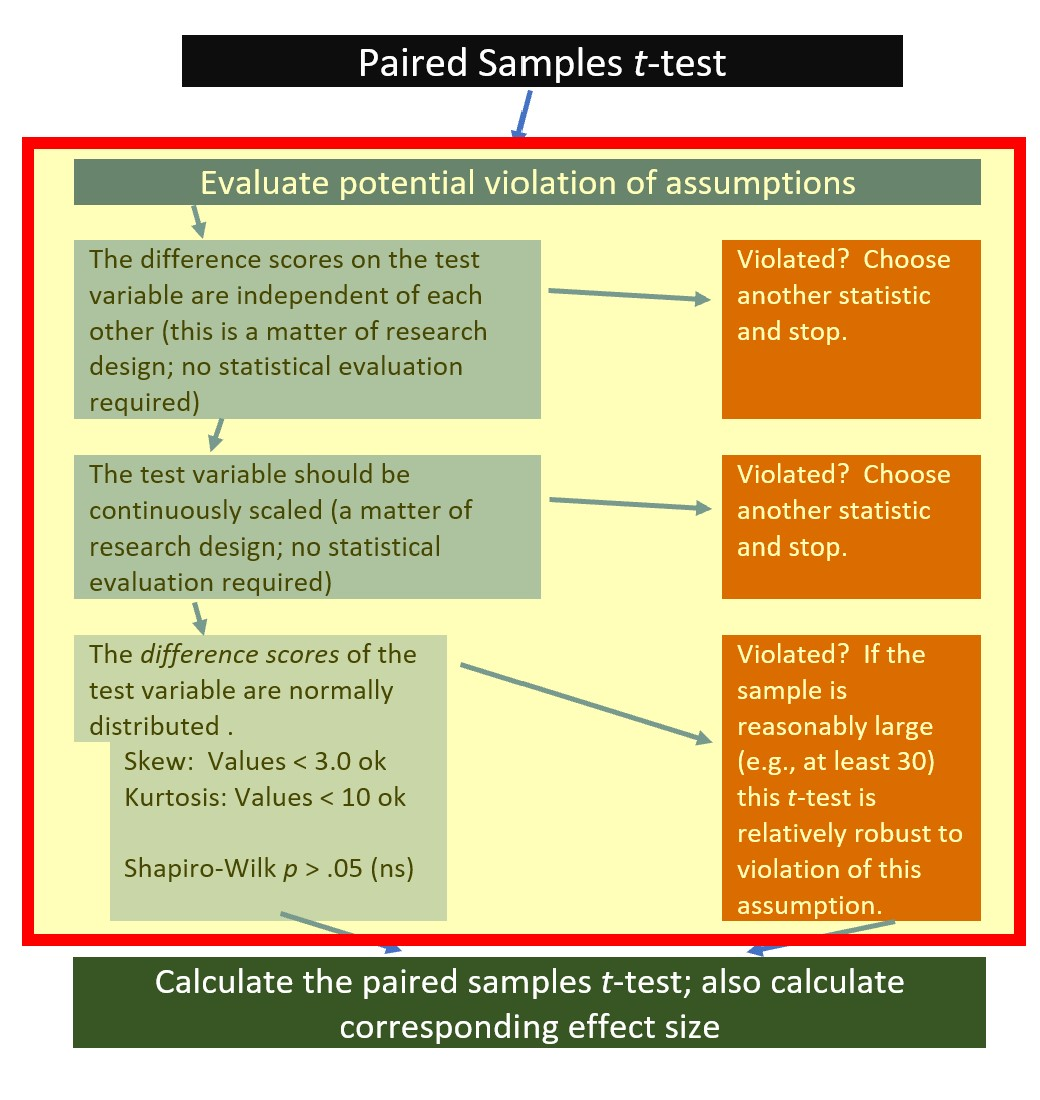
\includegraphics{images/ttests/PairedAssmptns.jpg} All statistical tests have some assumptions about the data. The paired-samples \emph{t}-test has three:

\begin{itemize}
\tightlist
\item
  The difference scores (i.e., the difference on the outcome across time or conditions) on the test variable are independent of each other. This is a matter of research design and no further statistical evaluation is required.
\item
  The test variable should be continuously scaled. This is also a matter of research design and no statistical analysis is required.

  \begin{itemize}
  \tightlist
  \item
    Our test variable is measured in minutes; this is continuously scaled and has the properties of \emph{interval}-level data.
  \end{itemize}
\item
  The \emph{difference scores} of the test variable are normally distributed. We can check this several ways:

  \begin{itemize}
  \tightlist
  \item
    visually with histograms (perhaps with superimposed curves) and boxplots,
  \item
    calculation of skew and kurtosis values,
  \item
    calculation of the Shapiro-Wilk test of normality
  \end{itemize}
\end{itemize}

\hypertarget{are-the-difference-scores-of-the-test-variable-normally-distributed}{%
\subsubsection{Are the difference scores of the test variable normally distributed?}\label{are-the-difference-scores-of-the-test-variable-normally-distributed}}

We can begin to evaluate normality by obtaining the descriptive statistics with the \emph{describe()} function from the \emph{psych} package.

\begin{Shaded}
\begin{Highlighting}[]
\NormalTok{psych}\SpecialCharTok{::}\FunctionTok{describe}\NormalTok{(dfPairedSamples, }\AttributeTok{type =} \DecValTok{1}\NormalTok{)}
\end{Highlighting}
\end{Shaded}

\begin{verbatim}
          vars  n  mean   sd median trimmed   mad   min   max range  skew
PhysID       1 33 17.00 9.67  17.00   17.00 11.86  1.00 33.00 32.00  0.00
Verbal_BL    2 33  8.70 2.80   9.09    8.80  3.10  1.94 13.34 11.40 -0.35
Verbal_WH    3 33  8.62 3.08   8.57    8.65  3.44  1.59 13.47 11.88 -0.15
NVerb_BL     4 33  2.73 1.00   2.63    2.78  1.26  0.43  4.23  3.80 -0.37
NVerb_WH     5 33  2.89 0.85   2.94    2.87  0.64  1.34  5.02  3.69  0.25
Verbal_D     6 33  0.08 4.14   0.61    0.27  4.11 -9.55  7.61 17.17 -0.42
          kurtosis   se
PhysID       -1.20 1.68
Verbal_BL    -0.31 0.49
Verbal_WH    -0.75 0.54
NVerb_BL     -0.71 0.17
NVerb_WH     -0.02 0.15
Verbal_D     -0.54 0.72
\end{verbatim}

We observe that the skew and kurtosis values for Verbal\_BL and Verbal\_WH are well below the areas of concern (below the absolute value of 3 for skew; below the absolute values of 10 for kurtosis) identified by Kline \citeyearpar{kline_data_2016}.

Recall, though that the normality assumption for the paired samples \emph{t}-test concerns the \emph{difference score} (Verbal\_D). We see that the mean difference is 0.08 (\emph{SD} = 4.14). Its skew (-0.42) and kurtosis (-0.54) are also well-below the thresholds of concern.

Beyond skew and kurtosis, we can formally test for deviations from normality with a Shapiro-Wilk. We want the results to be non-significant.

\begin{Shaded}
\begin{Highlighting}[]
\NormalTok{rstatix}\SpecialCharTok{::}\FunctionTok{shapiro\_test}\NormalTok{(dfPairedSamples, Verbal\_D)}
\end{Highlighting}
\end{Shaded}

\begin{verbatim}
# A tibble: 1 x 3
  variable statistic     p
  <chr>        <dbl> <dbl>
1 Verbal_D     0.973 0.572
\end{verbatim}

Results of the Shapiro-Wilk test of normality are not statistically significant \((W = 0.97, p = 0.57)\). This means that the distribution of difference scores is not statistically significantly different from a normal distribution.

\hypertarget{apa-style-write-up-of-testing-the-assumptions-1}{%
\subsubsection{APA style write-up of testing the assumptions}\label{apa-style-write-up-of-testing-the-assumptions-1}}

My practice is to create APA style drafts of the different sections of the analysis as I work along. Here's how I might capture our evaluation of the statistical assumptions:

\begin{quote}
We began by analyzing the data to see if it met the statistical assumptions for analysis with a paired samples \emph{t}-test. One assumption is that the difference scores of dependent variable are normally distributed. We evaluated skew and kurtosis using Kline's \citeyearpar{kline_data_2016} guidelines of the absolute values of 3 (skew) and 10 (kurtosis). Our results were well-within these boundary conditions. Further, a non-significant Shapiro-Wilk test of normality suggested that the distribution of difference scores was not statistically significant from a normal distribution \((W = 0.97, p = 0.57)\).
\end{quote}

\hypertarget{computing-the-paired-samples-t-test}{%
\subsection{\texorpdfstring{Computing the Paired Samples \emph{t}-Test}{Computing the Paired Samples t-Test}}\label{computing-the-paired-samples-t-test}}

We are ready to compute the paired samples \emph{t}-test.

\begin{figure}
\centering
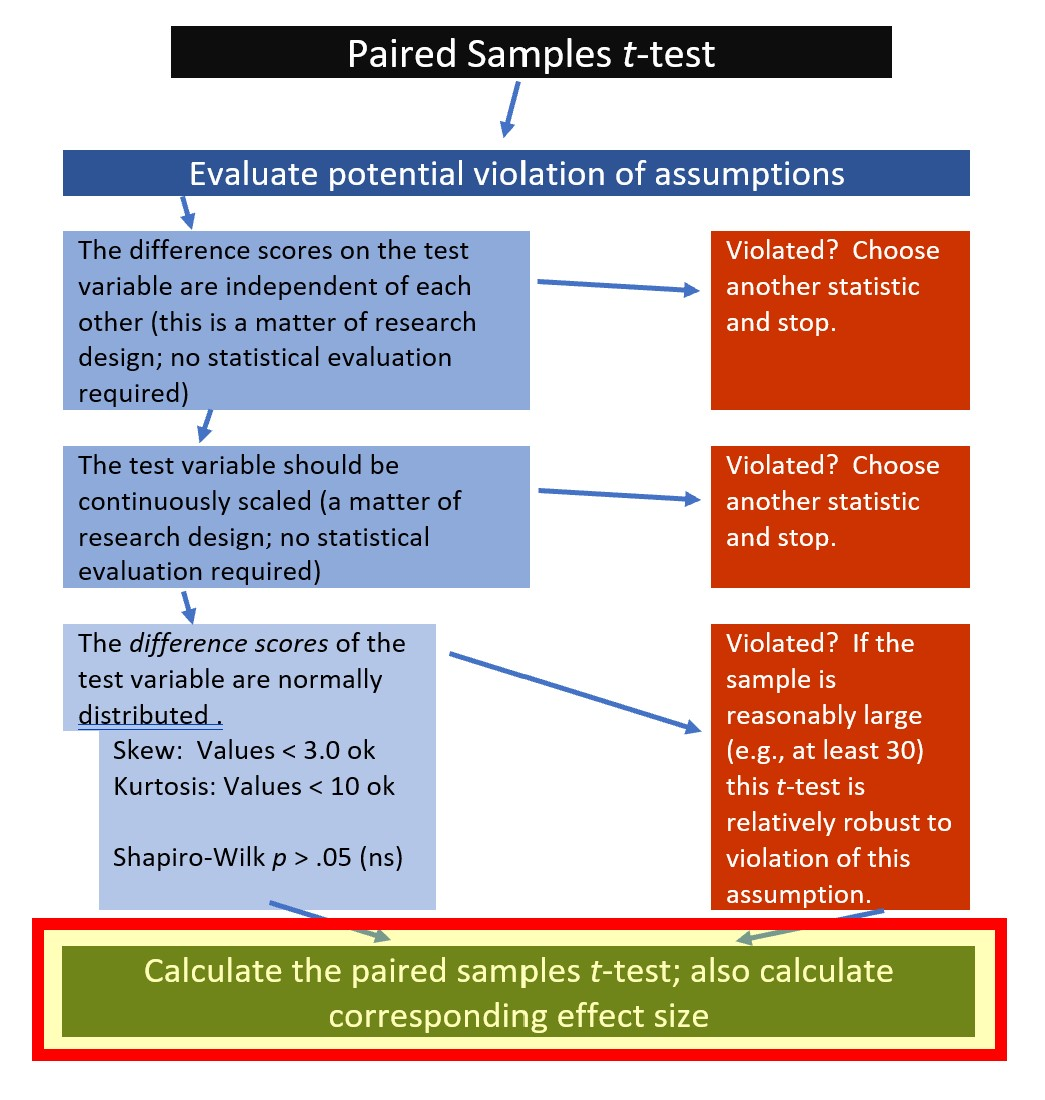
\includegraphics{images/ttests/PairedT.jpg}
\caption{A colorful image of a workflow for the paired samples \emph{t}-test}
\end{figure}

Calculating a paired samples \emph{t}-test is possible through base R and a number of packages. Kassambara's \citeyearpar{kassambara_pipe-friendly_nodate} \emph{rstatix} package is one we can use for all of the \emph{t}-test and ANOVA problems that we will work.

A challenge in evaluating within-persons data is the \emph{shape} of the data. The simulation resulted in a \emph{wide} (also termed person-level or multivariate) format, where each of the 33 physicians has the verbal and non-verbal communication scores with Black and White patients. We need to reshape the data to a long (also termed person-period or univariate) format. Although it may seem a bit tricky at first, this is a skill you will return to in many longitudinal or repeated measures analyses.

In the script below we are using the \emph{melt()} and \emph{setDT} functions from the \emph{data.table} package. We put stable (i.e., time-invarient, ``one-per-person'') variables in a concatonated variable list of ``id.vars.'' We create separate lists of the variables that change over time. In this case, each physician saw one Black patient and one White patient. Therefore, every physician will have two rows of data. For each variable collected at both points, we create concatonated lists.

\begin{Shaded}
\begin{Highlighting}[]
\NormalTok{df\_long }\OtherTok{\textless{}{-}}\NormalTok{ data.table}\SpecialCharTok{::}\FunctionTok{melt}\NormalTok{(data.table}\SpecialCharTok{::}\FunctionTok{setDT}\NormalTok{(dfPairedSamples), }\AttributeTok{id.vars =} \FunctionTok{c}\NormalTok{(}\StringTok{"PhysID"}\NormalTok{),}
    \AttributeTok{measure.vars =} \FunctionTok{list}\NormalTok{(}\FunctionTok{c}\NormalTok{(}\StringTok{"Verbal\_BL"}\NormalTok{, }\StringTok{"Verbal\_WH"}\NormalTok{), }\FunctionTok{c}\NormalTok{(}\StringTok{"NVerb\_BL"}\NormalTok{, }\StringTok{"NVerb\_WH"}\NormalTok{)))}
\FunctionTok{head}\NormalTok{(df\_long)}
\end{Highlighting}
\end{Shaded}

\begin{verbatim}
   PhysID variable    value1    value2
1:      1        1  8.190342 3.0991101
2:      2        1  3.297486 4.2338398
3:      3        1  6.176386 0.4288566
4:      4        1  4.851426 1.8347393
5:      5        1  6.911155 3.7035910
6:      6        1 11.965831 1.5369696
\end{verbatim}

While that code performed the magic, it did not name the variables. We must provide that in separate code.

\begin{Shaded}
\begin{Highlighting}[]
\NormalTok{df\_long }\OtherTok{\textless{}{-}} \FunctionTok{rename}\NormalTok{(df\_long, }\AttributeTok{PatientRace =}\NormalTok{ variable, }\AttributeTok{Verbal =}\NormalTok{ value1, }\AttributeTok{Nonverbal =}\NormalTok{ value2)}
\end{Highlighting}
\end{Shaded}

After the reshaping, let's recheck the structure of our data:

\begin{Shaded}
\begin{Highlighting}[]
\FunctionTok{str}\NormalTok{(df\_long)}
\end{Highlighting}
\end{Shaded}

\begin{verbatim}
Classes 'data.table' and 'data.frame':  66 obs. of  4 variables:
 $ PhysID     : int  1 2 3 4 5 6 7 8 9 10 ...
 $ PatientRace: Factor w/ 2 levels "1","2": 1 1 1 1 1 1 1 1 1 1 ...
 $ Verbal     : num  8.19 3.3 6.18 4.85 6.91 ...
 $ Nonverbal  : num  3.099 4.234 0.429 1.835 3.704 ...
 - attr(*, ".internal.selfref")=<externalptr> 
\end{verbatim}

The dependent variables Verbal and Nonverbal are continuously scaled, so the \emph{num} designation is appropriate. Similarly, PatientRace is categorical, so \emph{Factor} is appropriate. Because labels (instead of numbers) can minimize misinterpretation (or forgetting), I would prefer to use ``Black'' and ``White'' as opposed to ``1'' and ``2''. To further reduce the possibility of error, it is easy enough to create a second, parallel, variable.

\begin{Shaded}
\begin{Highlighting}[]
\NormalTok{df\_long}\SpecialCharTok{$}\NormalTok{PtRace }\OtherTok{\textless{}{-}}\NormalTok{ plyr}\SpecialCharTok{::}\FunctionTok{mapvalues}\NormalTok{(df\_long}\SpecialCharTok{$}\NormalTok{PatientRace, }\AttributeTok{from =} \FunctionTok{c}\NormalTok{(}\DecValTok{1}\NormalTok{, }\DecValTok{2}\NormalTok{),}
    \AttributeTok{to =} \FunctionTok{c}\NormalTok{(}\StringTok{"Black"}\NormalTok{, }\StringTok{"White"}\NormalTok{))}
\end{Highlighting}
\end{Shaded}

We are now ready to perform the paired samples \emph{t}-test. In the script below:

\begin{itemize}
\tightlist
\item
  the first element points to the dataframe
\item
  the second element provides a ``formula''

  \begin{itemize}
  \tightlist
  \item
    we are predicting ``Verbal'' from ``PtRace''
  \end{itemize}
\item
  specifying ``detailed = TRUE'' will produce the 95\% confidence interval around the difference
\end{itemize}

\begin{Shaded}
\begin{Highlighting}[]
\NormalTok{rstatix}\SpecialCharTok{::}\FunctionTok{t\_test}\NormalTok{(df\_long, Verbal }\SpecialCharTok{\textasciitilde{}}\NormalTok{ PtRace, }\AttributeTok{paired =} \ConstantTok{TRUE}\NormalTok{, }\AttributeTok{detailed =} \ConstantTok{TRUE}\NormalTok{)}
\end{Highlighting}
\end{Shaded}

\begin{verbatim}
# A tibble: 1 x 13
  estimate .y.    group1 group2    n1    n2 statistic     p    df conf.low
*    <dbl> <chr>  <chr>  <chr>  <int> <int>     <dbl> <dbl> <dbl>    <dbl>
1   0.0813 Verbal Black  White     33    33     0.113 0.911    32    -1.39
# i 3 more variables: conf.high <dbl>, method <chr>, alternative <chr>
\end{verbatim}

This output provides information to get us started in drafting the APA style results. Identical to all the information we hand-calculated, we would write the \emph{t} string this way: \(t(32) = 0.113, p = .911, CI95(-1.39, 1.55)\). Our results show that the mean difference in physician verbal communication scores with Black and White patients was 0.081. Taking a look at the confidence interval, we are 95\% confident that the true difference in means falls between the values of -1.386 and 1.549. What is critically important is that this confidence interval crosses zero. There is an important link between the CI95\% and statistical significance. When the CI95\% includes zero, \emph{p} will not be lower than 0.05.

We still need to calculate the effect size.

\begin{Shaded}
\begin{Highlighting}[]
\NormalTok{rstatix}\SpecialCharTok{::}\FunctionTok{cohens\_d}\NormalTok{(df\_long, Verbal }\SpecialCharTok{\textasciitilde{}}\NormalTok{ PtRace, }\AttributeTok{paired =} \ConstantTok{TRUE}\NormalTok{)}
\end{Highlighting}
\end{Shaded}

\begin{verbatim}
# A tibble: 1 x 7
  .y.    group1 group2 effsize    n1    n2 magnitude 
* <chr>  <chr>  <chr>    <dbl> <int> <int> <ord>     
1 Verbal Black  White   0.0196    33    33 negligible
\end{verbatim}

Keeping in mind the interpretive criteria of .2, .5, and .8, as small, medium, and large effect sizes, we see that \(d = 0.020\) is quite small. We can add it to our \emph{t}-string and draft the results: \(t(32) = 0.113, p = .911, d = 0.020, CI95(-1.39, 1.55)\).

\hypertarget{apa-style-results-2}{%
\section{APA Style Results}\label{apa-style-results-2}}

Putting it altogether we can assemble an APA style results section. Code for a table of means, standard deviations, and correlation follow the write-up of results. For inclusion in a manuscript, I would rework the export of the table to delete the difference score (i.e., Verbal\_D). I might also exclude the rows of confidence intervals around the correlations.

\begin{quote}
We began by analyzing the data to see if it met the statistical assumptions for analysis with a paired samples \emph{t}-test. One assumption is that the difference scores of dependent variable are normally distributed. We evaluated skew and kurtosis using Kline's \citeyearpar{kline_data_2016} guidelines of the absolute values of 3 (skew) and 10 (kurtosis). Our results were well-within these boundary conditions. Further, a non-significant Shapiro-Wilk test of normality suggested that the distribution of difference scores was not statistically significant from a normal distribution \((W = 0.97, p = 0.57)\).
\end{quote}

\begin{quote}
A paired samples \emph{t}-test was conducted to evaluate the hypothesis that there would be differences in the degree of physicians' verbal engagement as a function of the patient's race (Black, White). The paired samples \emph{t}-test was nonsignificant, \emph{t}(32) = 0.133, \emph{p} = .911. The small magnitude of the effect size (\emph{d} = 0.02) was consistent with the nonsignificant result. The 95\% confidence interval for the difference in means was quite wide and included the value of zero (95\%CI{[}-1.386, 1.549{]}). Means and standard deviations are presented in Table 1; the results are illustrated in Figure 1.
\end{quote}

\begin{Shaded}
\begin{Highlighting}[]
\FunctionTok{library}\NormalTok{(tidyverse)  }\CommentTok{\#needed to use the pipe }
\CommentTok{\# Creating a smaller df to include only the variables I want in the}
\CommentTok{\# table}
\NormalTok{PairedDescripts }\OtherTok{\textless{}{-}}\NormalTok{ dfPairedSamples }\SpecialCharTok{\%\textgreater{}\%}
    \FunctionTok{select}\NormalTok{(Verbal\_BL, Verbal\_WH, Verbal\_D)}
\CommentTok{\# using the apa.cor.table function for means, standard deviations,}
\CommentTok{\# and correlations the filename command will write the table as a}
\CommentTok{\# word document to your file}
\NormalTok{apaTables}\SpecialCharTok{::}\FunctionTok{apa.cor.table}\NormalTok{(PairedDescripts, }\AttributeTok{table.number =} \DecValTok{1}\NormalTok{, }\AttributeTok{filename =} \StringTok{"Tab1\_PairedV.doc"}\NormalTok{)}
\end{Highlighting}
\end{Shaded}

\begin{verbatim}


Table 1 

Means, standard deviations, and correlations with confidence intervals
 

  Variable     M    SD   1           2           
  1. Verbal_BL 8.70 2.80                         
                                                 
  2. Verbal_WH 8.62 3.08 .01                     
                         [-.33, .35]             
                                                 
  3. Verbal_D  0.08 4.14 .67**       -.74**      
                         [.42, .82]  [-.86, -.53]
                                                 

Note. M and SD are used to represent mean and standard deviation, respectively.
Values in square brackets indicate the 95% confidence interval.
The confidence interval is a plausible range of population correlations 
that could have caused the sample correlation (Cumming, 2014).
 * indicates p < .05. ** indicates p < .01.
 
\end{verbatim}

The figure we created earlier in the lesson would be sufficient for a journal article. However, using \emph{rstatix} in combination with \emph{ggpubbr} can be quite powerful. The result can be a figure that includes the \emph{t}-test results and ``significance bars.'' To do this, we first need to re-run the \emph{rstatix::t\_test}, but adding to it by

\begin{itemize}
\tightlist
\item
  including ``add\_significance()'' script after the pipe, and
\item
  saving it as an object, which I'm naming ``pair.test.''
\end{itemize}

We could have done this in the initial run (but I didn't want to make the test-statistic unnecessarily confusing).

\begin{Shaded}
\begin{Highlighting}[]
\FunctionTok{library}\NormalTok{(tidyverse)}
\NormalTok{pair.test }\OtherTok{\textless{}{-}}\NormalTok{ rstatix}\SpecialCharTok{::}\FunctionTok{t\_test}\NormalTok{(df\_long, Verbal }\SpecialCharTok{\textasciitilde{}}\NormalTok{ PtRace, }\AttributeTok{paired =} \ConstantTok{TRUE}\NormalTok{, }\AttributeTok{detailed =} \ConstantTok{TRUE}\NormalTok{) }\SpecialCharTok{\%\textgreater{}\%}
\NormalTok{    rstatix}\SpecialCharTok{::}\FunctionTok{add\_significance}\NormalTok{()}
\NormalTok{pair.test}
\end{Highlighting}
\end{Shaded}

\begin{verbatim}
# A tibble: 1 x 14
  estimate .y.    group1 group2    n1    n2 statistic     p    df conf.low
     <dbl> <chr>  <chr>  <chr>  <int> <int>     <dbl> <dbl> <dbl>    <dbl>
1   0.0813 Verbal Black  White     33    33     0.113 0.911    32    -1.39
# i 4 more variables: conf.high <dbl>, method <chr>, alternative <chr>,
#   p.signif <chr>
\end{verbatim}

Next, we create boxplot code with the long form of our data:

\begin{Shaded}
\begin{Highlighting}[]
\NormalTok{pair.box }\OtherTok{\textless{}{-}}\NormalTok{ ggpubr}\SpecialCharTok{::}\FunctionTok{ggpaired}\NormalTok{(df\_long, }\AttributeTok{x =} \StringTok{"PtRace"}\NormalTok{, }\AttributeTok{y =} \StringTok{"Verbal"}\NormalTok{, }\AttributeTok{order =} \FunctionTok{c}\NormalTok{(}\StringTok{"Black"}\NormalTok{,}
    \StringTok{"White"}\NormalTok{), }\AttributeTok{line.color =} \StringTok{"gray"}\NormalTok{, }\AttributeTok{palette =} \FunctionTok{c}\NormalTok{(}\StringTok{"npg"}\NormalTok{), }\AttributeTok{color =} \StringTok{"PtRace"}\NormalTok{,}
    \AttributeTok{ylab =} \StringTok{"Verbal Communication Rating"}\NormalTok{, }\AttributeTok{xlab =} \StringTok{"Patient Race"}\NormalTok{, }\AttributeTok{title =} \StringTok{"Figure 1. Physician Verbal Engagement as a Function of Patient Race"}\NormalTok{)}

\NormalTok{pair.test }\OtherTok{\textless{}{-}}\NormalTok{ pair.test }\SpecialCharTok{\%\textgreater{}\%}
\NormalTok{    rstatix}\SpecialCharTok{::}\FunctionTok{add\_xy\_position}\NormalTok{(}\AttributeTok{x =} \StringTok{"PtRace"}\NormalTok{)  }\CommentTok{\#autocomputes p{-}value labels positions}

\NormalTok{pair.box }\OtherTok{\textless{}{-}}\NormalTok{ pair.box }\SpecialCharTok{+}\NormalTok{ ggpubr}\SpecialCharTok{::}\FunctionTok{stat\_pvalue\_manual}\NormalTok{(pair.test, }\AttributeTok{tip.length =} \FloatTok{0.01}\NormalTok{,}
    \AttributeTok{y.position =} \FunctionTok{c}\NormalTok{(}\DecValTok{15}\NormalTok{)) }\SpecialCharTok{+} \FunctionTok{labs}\NormalTok{(}\AttributeTok{subtitle =}\NormalTok{ rstatix}\SpecialCharTok{::}\FunctionTok{get\_test\_label}\NormalTok{(pair.test,}
    \AttributeTok{detailed =} \ConstantTok{TRUE}\NormalTok{))}

\NormalTok{pair.box}
\end{Highlighting}
\end{Shaded}

\includegraphics{06-tPairedSamples_files/figure-latex/unnamed-chunk-27-1.pdf} The tools available offer a great deal of flexibility. Determining which figure is best will likely depend on your outlet, your audience, and your personal preferences. For example, a print journal might prefer a black-and-white figure (with no fill in the boxes). This is accomplished easily enough by removing (or, hashtagging out) the ``fill = PtRace'' argument.

\hypertarget{power-in-paired-samples-t-tests}{%
\section{\texorpdfstring{Power in Paired Samples \emph{t}-Tests}{Power in Paired Samples t-Tests}}\label{power-in-paired-samples-t-tests}}

Researchers often use power analysis packages to estimate the sample size needed to detect a statistically significant effect, if, in fact, there is one. Utilized another way, these tools allows us to determine the probability of detecting an effect of a given size with a given level of confidence. If the probability is unacceptably low, we may want to revise or stop. A helpful overview of power as well as guidelines for how to use the \emph{pwr} package can be found at a \href{https://www.statmethods.net/stats/power.html}{Quick-R website} \citep{kabacoff_power_2017}.

In Champely's \emph{pwr} package, we can conduct a power analysis for a variety of designs, including the paired \emph{t}-test that we worked in this chapter. There are a number of interrelating elements of power:

\begin{itemize}
\tightlist
\item
  Sample size, \emph{n} refers to the number of pairs; our vignette had 33
\item
  \emph{d} refers to the difference between means divided by the pooled standard deviation; we can use the value of Cohen's \emph{d} for this
\item
  \emph{power} refers to the power of a statistical test; conventionally it is set at .80
\item
  \emph{sig.level} refers to our desired alpha level; conventionally it is set at .05
\item
  \emph{type} indicates the type of test we ran; ours was ``paired''
\item
  \emph{alternative} refers to whether the hypothesis is non-directional/two-tailed (``two.sided'') or directional/one-tailed(``less'' or ``greater'')
\end{itemize}

In this script, we must specify \emph{all-but-one} parameter; the remaining parameter must be defined as NULL. R will calculate the value for the missing parameter.

When we conduct a ``power analysis'' (i.e., the likelihood of a hypothesis test detecting an effect if there is one), we specify, ``power=NULL''. Using the data from our results, we learn from this first run, that our statistical power was at 5\%. That is, given the low value of the mean difference (.08) and the relatively large standard deviation (4.14), we had only a 5\% chance of detecting a statistically significant effect if there was one.

\begin{Shaded}
\begin{Highlighting}[]
\NormalTok{pwr}\SpecialCharTok{::}\FunctionTok{pwr.t.test}\NormalTok{(}\AttributeTok{d =} \FloatTok{0.02}\NormalTok{, }\AttributeTok{n =} \DecValTok{33}\NormalTok{, }\AttributeTok{power =} \ConstantTok{NULL}\NormalTok{, }\AttributeTok{sig.level =} \FloatTok{0.05}\NormalTok{, }\AttributeTok{type =} \StringTok{"paired"}\NormalTok{,}
    \AttributeTok{alternative =} \StringTok{"two.sided"}\NormalTok{)}
\end{Highlighting}
\end{Shaded}

\begin{verbatim}

     Paired t test power calculation 

              n = 33
              d = 0.02
      sig.level = 0.05
          power = 0.05142498
    alternative = two.sided

NOTE: n is number of *pairs*
\end{verbatim}

The results indicate that we were powered at 5\%. That is, we had a 5\% chance of finding a statistically significant difference, if in fact there was one.

Researchers frequently use these tools to estimate the sample size required to obtain a statistically significant effect. In these scenarios we set \emph{n} to \emph{NULL}.

\begin{Shaded}
\begin{Highlighting}[]
\NormalTok{pwr}\SpecialCharTok{::}\FunctionTok{pwr.t.test}\NormalTok{(}\AttributeTok{d =} \FloatTok{0.02}\NormalTok{, }\AttributeTok{n =} \ConstantTok{NULL}\NormalTok{, }\AttributeTok{power =} \FloatTok{0.8}\NormalTok{, }\AttributeTok{sig.level =} \FloatTok{0.05}\NormalTok{, }\AttributeTok{type =} \StringTok{"paired"}\NormalTok{,}
    \AttributeTok{alternative =} \StringTok{"two.sided"}\NormalTok{)}
\end{Highlighting}
\end{Shaded}

\begin{verbatim}

     Paired t test power calculation 

              n = 19624.07
              d = 0.02
      sig.level = 0.05
          power = 0.8
    alternative = two.sided

NOTE: n is number of *pairs*
\end{verbatim}

Using the results from the simulation of our research vignette, you can see that we would have needed 19624 individuals for the \emph{p} value to be \textless{} .05, if, in fact there were a significant difference.

Let's see if this is true. Below I will re-simulate the data for the verbal scores, changing only the sample size:

\begin{Shaded}
\begin{Highlighting}[]
\FunctionTok{set.seed}\NormalTok{(}\DecValTok{220820}\NormalTok{)}
\CommentTok{\# These define the characteristics of the verbal variable. It is}
\CommentTok{\# essential that the object names (e.g., A\_mean) are not changed}
\CommentTok{\# because they will be fed to the function in the faux package.}
\NormalTok{sub\_n }\OtherTok{\textless{}{-}} \DecValTok{19624}
\NormalTok{A\_mean }\OtherTok{\textless{}{-}} \FloatTok{8.37}
\NormalTok{B\_mean }\OtherTok{\textless{}{-}} \FloatTok{8.41}
\NormalTok{A\_sd }\OtherTok{\textless{}{-}} \FloatTok{3.36}
\NormalTok{B\_sd }\OtherTok{\textless{}{-}} \FloatTok{3.21}
\NormalTok{AB\_r }\OtherTok{\textless{}{-}} \FloatTok{0.3}

\CommentTok{\# the faux package can simulate a variety of data. This function}
\CommentTok{\# within the faux package will use the objects above to simulate}
\CommentTok{\# paired samples data}
\NormalTok{paired\_V2 }\OtherTok{\textless{}{-}}\NormalTok{ faux}\SpecialCharTok{::}\FunctionTok{rnorm\_multi}\NormalTok{(}\AttributeTok{n =}\NormalTok{ sub\_n, }\AttributeTok{vars =} \DecValTok{2}\NormalTok{, }\AttributeTok{r =}\NormalTok{ AB\_r, }\AttributeTok{mu =} \FunctionTok{c}\NormalTok{(A\_mean,}
\NormalTok{    B\_mean), }\AttributeTok{sd =} \FunctionTok{c}\NormalTok{(A\_sd, B\_sd), }\AttributeTok{varnames =} \FunctionTok{c}\NormalTok{(}\StringTok{"Verbal\_BL"}\NormalTok{, }\StringTok{"Verbal\_WH"}\NormalTok{))}

\NormalTok{paired\_V2 }\OtherTok{\textless{}{-}}\NormalTok{ paired\_V2 }\SpecialCharTok{\%\textgreater{}\%}
\NormalTok{    dplyr}\SpecialCharTok{::}\FunctionTok{mutate}\NormalTok{(}\AttributeTok{PhysID =} \FunctionTok{row\_number}\NormalTok{())}

\CommentTok{\# restructuring data to the long form}
\NormalTok{df\_longV2 }\OtherTok{\textless{}{-}}\NormalTok{ data.table}\SpecialCharTok{::}\FunctionTok{melt}\NormalTok{(data.table}\SpecialCharTok{::}\FunctionTok{setDT}\NormalTok{(paired\_V2), }\AttributeTok{id.vars =} \FunctionTok{c}\NormalTok{(}\StringTok{"PhysID"}\NormalTok{),}
    \AttributeTok{measure.vars =} \FunctionTok{list}\NormalTok{(}\FunctionTok{c}\NormalTok{(}\StringTok{"Verbal\_BL"}\NormalTok{, }\StringTok{"Verbal\_WH"}\NormalTok{)))}
\NormalTok{df\_longV2 }\OtherTok{\textless{}{-}} \FunctionTok{rename}\NormalTok{(df\_longV2, }\AttributeTok{PatientRace =}\NormalTok{ variable, }\AttributeTok{Verbal =}\NormalTok{ value)}
\NormalTok{df\_longV2}\SpecialCharTok{$}\NormalTok{PtRace }\OtherTok{\textless{}{-}}\NormalTok{ plyr}\SpecialCharTok{::}\FunctionTok{mapvalues}\NormalTok{(df\_longV2}\SpecialCharTok{$}\NormalTok{PatientRace, }\AttributeTok{from =} \FunctionTok{c}\NormalTok{(}\StringTok{"Verbal\_BL"}\NormalTok{,}
    \StringTok{"Verbal\_WH"}\NormalTok{), }\AttributeTok{to =} \FunctionTok{c}\NormalTok{(}\StringTok{"Black"}\NormalTok{, }\StringTok{"White"}\NormalTok{))}
\end{Highlighting}
\end{Shaded}

Now I will conduct the paired samples \emph{t}-test and corresponding effect size.

\begin{Shaded}
\begin{Highlighting}[]
\NormalTok{rstatix}\SpecialCharTok{::}\FunctionTok{t\_test}\NormalTok{(df\_longV2, Verbal }\SpecialCharTok{\textasciitilde{}}\NormalTok{ PtRace, }\AttributeTok{paired =} \ConstantTok{TRUE}\NormalTok{, }\AttributeTok{detailed =} \ConstantTok{TRUE}\NormalTok{)}
\end{Highlighting}
\end{Shaded}

\begin{verbatim}
# A tibble: 1 x 13
  estimate .y.    group1 group2    n1    n2 statistic     p    df conf.low
*    <dbl> <chr>  <chr>  <chr>  <int> <int>     <dbl> <dbl> <dbl>    <dbl>
1  -0.0343 Verbal Black  White  19624 19624     -1.24 0.214 19623  -0.0885
# i 3 more variables: conf.high <dbl>, method <chr>, alternative <chr>
\end{verbatim}

\begin{Shaded}
\begin{Highlighting}[]
\NormalTok{rstatix}\SpecialCharTok{::}\FunctionTok{cohens\_d}\NormalTok{(df\_longV2, Verbal }\SpecialCharTok{\textasciitilde{}}\NormalTok{ PtRace, }\AttributeTok{paired =} \ConstantTok{TRUE}\NormalTok{)}
\end{Highlighting}
\end{Shaded}

\begin{verbatim}
# A tibble: 1 x 7
  .y.    group1 group2  effsize    n1    n2 magnitude 
* <chr>  <chr>  <chr>     <dbl> <int> <int> <ord>     
1 Verbal Black  White  -0.00887 19624 19624 negligible
\end{verbatim}

The new results remain non-significant: \(t(19623) = -1.243, p = 0.241, d = -0.009, 95CI (-0.088, 0.020)\). This tells me these means are quite similar and this is not a function of being under powered.

Conducting power analyses requires that researchers speculate about their values. In this case, in order to estimate sample size, the researcher would need to make some guesses about the difference scores means and standard deviations. These values could be estimated from prior literature or a pilot study.

\hypertarget{practice-problems-4}{%
\section{Practice Problems}\label{practice-problems-4}}

The suggestions for homework differ in degree of complexity. I encourage you to start with a problem that feels ``do-able'' and then try at least one more problem that challenges you in some way. Regardless, your choices should meet you where you are (e.g., in terms of your self-efficacy for statistics, your learning goals, and competing life demands).

Additionally, please complete at least one set of \emph{hand calculations}, that is use the code demonstrated in the chapter to work through the formulas that compute the paired samples \emph{t}-test. At this stage in your learning, you may ignore any missingness in your dataset by excluding all rows with missing data in your variables of interest.

\hypertarget{problem-1-rework-the-research-vignette-as-demonstrated-but-change-the-random-seed-2}{%
\subsection{Problem \#1: Rework the research vignette as demonstrated, but change the random seed}\label{problem-1-rework-the-research-vignette-as-demonstrated-but-change-the-random-seed-2}}

If this topic feels a bit overwhelming, simply change the random seed in the data simulation of the research vignette, then rework the problem. This should provide minor changes to the data (maybe even in the second or third decimal point), but the results will likely be very similar. That said, don't be alarmed if what was non-significant in my working of the problem becomes significant. Our selection of \emph{p} \textless{} .05 (and the corresponding 95\% confidence interval) means that 5\% of the time there could be a difference in statistical significance.

\hypertarget{problem-2-rework-the-research-vignette-but-change-something-about-the-simulation-2}{%
\subsection{Problem \#2: Rework the research vignette, but change something about the simulation}\label{problem-2-rework-the-research-vignette-but-change-something-about-the-simulation-2}}

Rework the paired samples \emph{t}-test in the lesson by changing something else about the simulation. For example, if you are interested in understanding more about power, consider changing the sample size. Alternatively, you could specify different means and/or standard deviations.

\hypertarget{problem-3-rework-the-research-vignette-but-swap-one-or-more-variables-1}{%
\subsection{Problem \#3: Rework the research vignette, but swap one or more variables}\label{problem-3-rework-the-research-vignette-but-swap-one-or-more-variables-1}}

Use the simulated data, but select the nonverbal communication variables that were evaluated in the Elliott et al. \citeyearpar{elliott_differences_2016} study. Compare your results to those reported in the mansucript.

\hypertarget{problem-4-use-other-data-that-is-available-to-you-1}{%
\subsection{Problem \#4: Use other data that is available to you}\label{problem-4-use-other-data-that-is-available-to-you-1}}

Using data for which you have permission and access (e.g., IRB approved data you have collected or from your lab; data you simulate from a published article; data from an open science repository; data from other chapters in this OER), complete a paired samples \emph{t}-test.

\hypertarget{grading-rubric-2}{%
\subsection{Grading Rubric}\label{grading-rubric-2}}

Regardless which option(s) you chose, use the elements in the grading rubric to guide you through the practice.

\begin{longtable}[]{@{}
  >{\raggedright\arraybackslash}p{(\columnwidth - 4\tabcolsep) * \real{0.5493}}
  >{\centering\arraybackslash}p{(\columnwidth - 4\tabcolsep) * \real{0.2535}}
  >{\centering\arraybackslash}p{(\columnwidth - 4\tabcolsep) * \real{0.1972}}@{}}
\toprule\noalign{}
\begin{minipage}[b]{\linewidth}\raggedright
Assignment Component
\end{minipage} & \begin{minipage}[b]{\linewidth}\centering
Points Possible
\end{minipage} & \begin{minipage}[b]{\linewidth}\centering
Points Earned
\end{minipage} \\
\midrule\noalign{}
\endhead
\bottomrule\noalign{}
\endlastfoot
1. Narrate the research vignette, describing the variables and their role in the analysis & 5 & \_\_\_\_\_ \\
2. Simulate (or import) and format data & 5 & \_\_\_\_\_ \\
3. Evaluate statistical assumptions & 5 & \_\_\_\_\_ \\
4. Conduct a paired samples \emph{t}-test (with an effect size \& 95\%CIs) & 5 & \_\_\_\_\_ \\
5. APA style results with table(s) and figure & 5 & \_\_\_\_\_ \\
6. Conduct power analyses to determine the power of the current study and a recommended sample size & 5 & \_\_\_\_\_ \\
7. Explanation to grader & 5 & \_\_\_\_\_ \\
\textbf{Totals} & 35 & \_\_\_\_\_ \\
\end{longtable}

\begin{longtable}[]{@{}
  >{\raggedright\arraybackslash}p{(\columnwidth - 4\tabcolsep) * \real{0.5833}}
  >{\centering\arraybackslash}p{(\columnwidth - 4\tabcolsep) * \real{0.2083}}
  >{\raggedright\arraybackslash}p{(\columnwidth - 4\tabcolsep) * \real{0.2083}}@{}}
\toprule\noalign{}
\begin{minipage}[b]{\linewidth}\raggedright
Hand Calculations
\end{minipage} & \begin{minipage}[b]{\linewidth}\centering
Points Poss
\end{minipage} & \begin{minipage}[b]{\linewidth}\raggedright
Points Earned
\end{minipage} \\
\midrule\noalign{}
\endhead
\bottomrule\noalign{}
\endlastfoot
1. Using traditional NHST (null hypothesis testing language), state your null and alternative hypotheses & 2 & \\
2. Using an R package or functions in base R (and with data in the ``wide'' format), calculate the \emph{difference} score between the two observations of the dependent variable & 2 & \\
3. Obtain the mean and standard deviation of the \emph{difference} score & 2 & \\
4. Calculate the paired samples \emph{t}-test & 4 & \\
5. Identify the degrees of freedom associated with your paired samples \emph{t}-test & 2 & \\
6. Locate the test critical value for your paired samples \emph{t}-test & 2 & \\
7. Is the paired samples \emph{t}-test statistically significant? Why or why not? & 2 & \\
8. What is the confidence interval around the mean difference? & 4 & \\
9. Calculate the effect size (i.e., Cohen's \emph{d} associated with your paired samples \emph{t}-test & 4 & \\
10. Assemble the results into a statistical string & 4 & \\
\textbf{Totals* } & 28 & \\
\end{longtable}

\hypertarget{homeworked-example-4}{%
\section{Homeworked Example}\label{homeworked-example-4}}

\href{link}{Screencast Link}

\emph{If you wanted to use this example and dataset as a basis for a homework assignment, you could compare a differenc combination of courses and/or score one of the other course evaluation subscales (e.g., socially responsive pedagogy or valued-by-me). }

\hypertarget{working-the-problem-with-r-and-r-packages-3}{%
\subsection{Working the Problem with R and R Packages}\label{working-the-problem-with-r-and-r-packages-3}}

\hypertarget{narrate-the-research-vignette-describing-the-variables-and-their-role-in-the-analysis-2}{%
\subsubsection{Narrate the research vignette, describing the variables and their role in the analysis}\label{narrate-the-research-vignette-describing-the-variables-and-their-role-in-the-analysis-2}}

I want to ask the question, ``Do students' evaluations of traditional pedagogy (TradPed) change from ANOVA (the first course in the series) to Multivariate (the second course in the series)?.'' Unlike the independent samples \emph{t}-test where we compared students in two different departments, we are comparing \emph{the same} students across two different conditions. In this particular analysis, there is also an element of time. That is the ANOVA class always precedes the multivariate class (with a regression class, taught by a different instructor) in the intervening academic quarter.

This research design has some clear limitations. Threats to internal validity are caused by issues like history and maturation. None-the-less, for the purpose of a statistical demonstration, this dataset works.

Like most data, some manipulation is required before we can begin the analyses.

\hypertarget{simulate-or-import-and-format-data-2}{%
\subsubsection{Simulate (or import) and format data}\label{simulate-or-import-and-format-data-2}}

Let's import the larger dataset.

\begin{Shaded}
\begin{Highlighting}[]
\NormalTok{larger }\OtherTok{\textless{}{-}} \FunctionTok{readRDS}\NormalTok{(}\StringTok{"ReC.rds"}\NormalTok{)}
\end{Highlighting}
\end{Shaded}

The TradPed (traditional pedagogy) variable is an average of the items on that scale. I will first create that variable.

\begin{Shaded}
\begin{Highlighting}[]
\CommentTok{\#Creates a list of the variables that belong to that scale}
\NormalTok{TradPed\_vars }\OtherTok{\textless{}{-}} \FunctionTok{c}\NormalTok{(}\StringTok{\textquotesingle{}ClearResponsibilities\textquotesingle{}}\NormalTok{, }\StringTok{\textquotesingle{}EffectiveAnswers\textquotesingle{}}\NormalTok{,}\StringTok{\textquotesingle{}Feedback\textquotesingle{}}\NormalTok{, }\StringTok{\textquotesingle{}ClearOrganization\textquotesingle{}}\NormalTok{,}\StringTok{\textquotesingle{}ClearPresentation\textquotesingle{}}\NormalTok{)}

\CommentTok{\#Calculates a mean if at least 75\% of the items are non{-}missing; adjusts the calculating when there is missingness}
\NormalTok{larger}\SpecialCharTok{$}\NormalTok{TradPed }\OtherTok{\textless{}{-}}\NormalTok{ sjstats}\SpecialCharTok{::}\FunctionTok{mean\_n}\NormalTok{(larger[, ..TradPed\_vars], .}\DecValTok{75}\NormalTok{)}
\end{Highlighting}
\end{Shaded}

From the ``larger'' data, let's select only the variable we will use in the analysis. I have included ``long'' in the filename because the structure of the dataset is that course evaluation by each student is in its own row. That is, each student could have up to three rows of data.

We need both ``long'' and ``wide'' forms to conduct the analyses required for both testing the statistical assumptions and performing the paired samples \emph{t}-test.

\begin{Shaded}
\begin{Highlighting}[]
\NormalTok{paired\_long }\OtherTok{\textless{}{-}}\NormalTok{(dplyr}\SpecialCharTok{::}\FunctionTok{select}\NormalTok{ (larger, deID, Course, TradPed))}
\end{Highlighting}
\end{Shaded}

From that reduced variable set, let's create a subset with students only from those two courses.

\begin{Shaded}
\begin{Highlighting}[]
\NormalTok{paired\_long }\OtherTok{\textless{}{-}} \FunctionTok{subset}\NormalTok{(paired\_long, Course }\SpecialCharTok{==} \StringTok{"ANOVA"} \SpecialCharTok{|}\NormalTok{ Course }\SpecialCharTok{==} \StringTok{"Multivariate"}\NormalTok{) }
\end{Highlighting}
\end{Shaded}

Regarding the structure of the data, we want the conditions (ANOVA, multivariate) to be factors and the TradPed variable to be continuously scaled. The format of the deID variable can be any numerical or categorical format -- just not a ``chr'' (character) variable.

\begin{Shaded}
\begin{Highlighting}[]
\FunctionTok{str}\NormalTok{(paired\_long)}
\end{Highlighting}
\end{Shaded}

\begin{verbatim}
Classes 'data.table' and 'data.frame':  198 obs. of  3 variables:
 $ deID   : int  1 2 3 4 5 6 7 8 9 10 ...
 $ Course : Factor w/ 3 levels "Psychometrics",..: 2 2 2 2 2 2 2 2 2 2 ...
 $ TradPed: num  4.4 3.8 4 3 4.8 3.5 4.6 3.8 3.6 4.6 ...
 - attr(*, ".internal.selfref")=<externalptr> 
\end{verbatim}

R correctly interpreted our variables.

For analyzing the assumptions associated with the paired-samples \emph{t}-test, the format needs to be ``wide'' form (where each student has both observations on one row). Our data is presently in ``long'' form (where each observation is listed in each row). Here's how to reshape the data.

\begin{Shaded}
\begin{Highlighting}[]
\NormalTok{paired\_wide }\OtherTok{\textless{}{-}}\NormalTok{ reshape2}\SpecialCharTok{::}\FunctionTok{dcast}\NormalTok{(}\AttributeTok{data =}\NormalTok{ paired\_long, }\AttributeTok{formula =}\NormalTok{deID }\SpecialCharTok{\textasciitilde{}}\NormalTok{ Course, }\AttributeTok{value.var =} \StringTok{"TradPed"}\NormalTok{)}
\end{Highlighting}
\end{Shaded}

Let's recheck the structure.

\begin{Shaded}
\begin{Highlighting}[]
\FunctionTok{str}\NormalTok{(paired\_wide)}
\end{Highlighting}
\end{Shaded}

\begin{verbatim}
'data.frame':   119 obs. of  3 variables:
 $ deID        : int  1 2 3 4 5 6 7 8 9 10 ...
 $ ANOVA       : num  4.4 3.8 4 3 4.8 3.5 4.6 3.8 3.6 4.6 ...
 $ Multivariate: num  NA NA NA NA NA NA NA NA NA NA ...
\end{verbatim}

You will notice that there is a good deal of missingness in the Multivariate condition. This is caused because the most recent cohort of students had not yet taken the course. While managing missingness is more complex than this, for the sake of simplicity, I will create a dataframe with non-missing data.

Doing so should also help with the hand-calculations later in the worked example.

\begin{Shaded}
\begin{Highlighting}[]
\NormalTok{paired\_wide }\OtherTok{\textless{}{-}} \FunctionTok{na.omit}\NormalTok{(paired\_wide)}
\end{Highlighting}
\end{Shaded}

\hypertarget{evaluate-statistical-assumptions-2}{%
\subsubsection{Evaluate statistical assumptions}\label{evaluate-statistical-assumptions-2}}

We need to evaluate the \emph{distribution of the difference score} in terms of skew and kurtosis. We want this distribution of difference scores to be normally distributed.

This means we need to create a difference score:

\begin{Shaded}
\begin{Highlighting}[]
\NormalTok{paired\_wide}\SpecialCharTok{$}\NormalTok{DIFF }\OtherTok{\textless{}{-}}\NormalTok{ paired\_wide}\SpecialCharTok{$}\NormalTok{ANOVA }\SpecialCharTok{{-}}\NormalTok{ paired\_wide}\SpecialCharTok{$}\NormalTok{Multivariate}
\end{Highlighting}
\end{Shaded}

We can use the \emph{psych::describe()} function to obtain skew and kurtosis.

\begin{Shaded}
\begin{Highlighting}[]
\NormalTok{psych}\SpecialCharTok{::}\FunctionTok{describe}\NormalTok{(paired\_wide)}
\end{Highlighting}
\end{Shaded}

\begin{verbatim}
             vars  n  mean    sd median trimmed   mad  min   max range  skew
deID            1 77 62.27 35.43   60.0   59.54 34.10 11.0 142.0 131.0  0.63
ANOVA           2 77  4.21  0.73    4.2    4.29  0.89  2.2   5.0   2.8 -0.79
Multivariate    3 77  4.33  0.73    4.4    4.45  0.59  1.2   5.0   3.8 -1.90
DIFF            4 77 -0.12  0.80   -0.2   -0.13  0.59 -2.4   3.2   5.6  0.56
             kurtosis   se
deID            -0.40 4.04
ANOVA           -0.19 0.08
Multivariate     5.00 0.08
DIFF             3.15 0.09
\end{verbatim}

Regarding the DIFF score, the skew (0.56) and kurtosis (3.15) values were well below the threshholds of concern identified by Klein (2016).

We can formally test for deviations from normality with a Shapiro-Wilk. We want the results to be non-significant.

\begin{Shaded}
\begin{Highlighting}[]
\NormalTok{rstatix}\SpecialCharTok{::}\FunctionTok{shapiro\_test}\NormalTok{(paired\_wide, DIFF)}
\end{Highlighting}
\end{Shaded}

\begin{verbatim}
# A tibble: 1 x 3
  variable statistic       p
  <chr>        <dbl>   <dbl>
1 DIFF         0.943 0.00187
\end{verbatim}

Results of the Shapiro-Wilk test of normality are statistically significant \((W = 0.943, p = 0.002)\). This means that the distribution of difference scores are statistically significantly different from a normal distribution.

although not required in the formal test of instructions, a \emph{pairs panel} of correlations and distributions can be useful in undersatnding our data.

\begin{Shaded}
\begin{Highlighting}[]
\NormalTok{psych}\SpecialCharTok{::}\FunctionTok{pairs.panels}\NormalTok{(paired\_wide)}
\end{Highlighting}
\end{Shaded}

\includegraphics{06-tPairedSamples_files/figure-latex/unnamed-chunk-45-1.pdf} Visual inspection of the distributions of the specific course variables were negatively skewed, with values clustered at the high end of the course evaluation ratings. However, the distribution for the DIFF variable seems relatively normal (although maybe a bit leptokurtic). This is consistent with the statistically significant Shapiro-Wilk test.

Before moving forward, I want to capture my analysis of assumptions:

\begin{quote}
We began by analyzing the data to see if it met the statistical assumptions for analysis with a paired samples t-test. Regarding the assumption of normality, the skew (0.56) and kurtosis (3.15) values associated with the difference between conditions (ANOVA and multivariate) were below the threshholds of concern identified by Klein (2016). In contrast, results of the Shapiro-Wilk test of normality suggested that the distribution of difference scores was statistically significantly different than a normal distribution \((W = 0.943, p = 0.002)\).
\end{quote}

\hypertarget{conduct-a-paired-samples-t-test-with-an-effect-size-95-cis}{%
\subsubsection{Conduct a paired samples t-test (with an effect size \& 95\% CIs)}\label{conduct-a-paired-samples-t-test-with-an-effect-size-95-cis}}

So this may be a bit tricky, but our original ``long'' form of the data has more ANOVA evaluations (students who had taken ANOVA had not yet taken multivariate) than multivariate. The paired samples \emph{t} test requires the design to be balanced. When we used the \emph{na.omit()} function with the wide case, we effectively balanced the design, eliminating students who lacked observations across both courses. Let's restructure that wide format back to long format so that the design will be balanced.

\begin{Shaded}
\begin{Highlighting}[]
\NormalTok{paired\_long2 }\OtherTok{\textless{}{-}}\NormalTok{ data.table}\SpecialCharTok{::}\FunctionTok{melt}\NormalTok{(data.table}\SpecialCharTok{::}\FunctionTok{setDT}\NormalTok{(paired\_wide), }\AttributeTok{id.vars =} \FunctionTok{c}\NormalTok{(}\StringTok{"deID"}\NormalTok{),}
    \AttributeTok{measure.vars =} \FunctionTok{list}\NormalTok{(}\FunctionTok{c}\NormalTok{(}\StringTok{"ANOVA"}\NormalTok{, }\StringTok{"Multivariate"}\NormalTok{)))}

\NormalTok{paired\_long2 }\OtherTok{\textless{}{-}}\NormalTok{ dplyr}\SpecialCharTok{::}\FunctionTok{rename}\NormalTok{(paired\_long2, }\AttributeTok{Course =}\NormalTok{ variable, }\AttributeTok{TradPed =}\NormalTok{ value)}

\FunctionTok{head}\NormalTok{(paired\_long2)}
\end{Highlighting}
\end{Shaded}

\begin{verbatim}
   deID Course TradPed
1:   11  ANOVA     4.0
2:   12  ANOVA     4.2
3:   13  ANOVA     3.6
4:   14  ANOVA     3.6
5:   15  ANOVA     3.4
6:   16  ANOVA     2.2
\end{verbatim}

\begin{Shaded}
\begin{Highlighting}[]
\NormalTok{rstatix}\SpecialCharTok{::}\FunctionTok{t\_test}\NormalTok{(paired\_long2, TradPed }\SpecialCharTok{\textasciitilde{}}\NormalTok{ Course, }\AttributeTok{paired =} \ConstantTok{TRUE}\NormalTok{, }\AttributeTok{detailed =} \ConstantTok{TRUE}\NormalTok{)}
\end{Highlighting}
\end{Shaded}

\begin{verbatim}
# A tibble: 1 x 13
  estimate .y.     group1 group2         n1    n2 statistic     p    df conf.low
*    <dbl> <chr>   <chr>  <chr>       <int> <int>     <dbl> <dbl> <dbl>    <dbl>
1   -0.123 TradPed ANOVA  Multivaria~    77    77     -1.34 0.184    76   -0.305
# i 3 more variables: conf.high <dbl>, method <chr>, alternative <chr>
\end{verbatim}

I'll begin the \emph{t} string with this output: \(t(76) = -1.341, p = 0.184, CI95(-0.305, 0.069)\). The difference in course evaluations is not statistically significantly difference. We are 955 confident that the true difference in means is as low as -0.301 or as high as 0.060.

we calculate the Cohen's \emph{d} (the effect size) this way:

\begin{Shaded}
\begin{Highlighting}[]
\NormalTok{rstatix}\SpecialCharTok{::}\FunctionTok{cohens\_d}\NormalTok{(paired\_long2, TradPed }\SpecialCharTok{\textasciitilde{}}\NormalTok{ Course, }\AttributeTok{paired =} \ConstantTok{TRUE}\NormalTok{)}
\end{Highlighting}
\end{Shaded}

\begin{verbatim}
# A tibble: 1 x 7
  .y.     group1 group2       effsize    n1    n2 magnitude 
* <chr>   <chr>  <chr>          <dbl> <int> <int> <ord>     
1 TradPed ANOVA  Multivariate  -0.153    77    77 negligible
\end{verbatim}

The value of -0.153 is quite small. We can add this value to our statistical string: \(t(76) = -1.341, p = 0.184, CI95(-0.305, 0.069), d = -0.153\)

\hypertarget{apa-style-results-with-tables-and-figure-2}{%
\subsubsection{APA style results with table(s) and figure}\label{apa-style-results-with-tables-and-figure-2}}

\begin{quote}
A paired samples \emph{t}-test was conducted to evaluate the hypohtesis that there would be statistically significant differences in students' course evaluations of ANOVA and multivariate statistics classses.
\end{quote}

\begin{quote}
We began by analyzing the data to see if it met the statistical assumptions for analysis with a paired samples t-test. Regarding the assumption of normality, the skew (0.56) and kurtosis (3.15) values associated with the difference between conditions (ANOVA and multivariate) were below the threshholds of concern identified by Klein (2016). In contrast, results of the Shapiro-Wilk test of normality suggested that the distribution of difference scores was statistically significantly different than a normal distribution \$(W=0.943, p = 0.002)
\end{quote}

\begin{quote}
Results of the paired samples \emph{t}-test suggested nonsignificant differences \(t(76) = -1.341, p = 0.184,d = -0.153\). The 95\% confidence interval crossed zero, ranging from -0.305 to 0.069. Means and standard deviations are presented in Table 1 and illustrated in Figure 1.
\end{quote}

\begin{Shaded}
\begin{Highlighting}[]
\FunctionTok{library}\NormalTok{(tidyverse)  }\CommentTok{\#needed to use the pipe }
\CommentTok{\# Creating a smaller df to include only the variables I want in the}
\CommentTok{\# table}
\NormalTok{Descripts\_paired }\OtherTok{\textless{}{-}}\NormalTok{ paired\_wide }\SpecialCharTok{\%\textgreater{}\%}
    \FunctionTok{select}\NormalTok{(ANOVA, Multivariate, DIFF)}
\CommentTok{\# using the apa.cor.table function for means, standard deviations,}
\CommentTok{\# and correlations the filename command will write the table as a}
\CommentTok{\# word document to your file}
\NormalTok{apaTables}\SpecialCharTok{::}\FunctionTok{apa.cor.table}\NormalTok{(Descripts\_paired, }\AttributeTok{table.number =} \DecValTok{1}\NormalTok{, }\AttributeTok{filename =} \StringTok{"Tab1\_PairedT.doc"}\NormalTok{)}
\end{Highlighting}
\end{Shaded}

\begin{verbatim}


Table 1 

Means, standard deviations, and correlations with confidence intervals
 

  Variable        M     SD   1          2           
  1. ANOVA        4.21  0.73                        
                                                    
  2. Multivariate 4.33  0.73 .39**                  
                             [.18, .56]             
                                                    
  3. DIFF         -0.12 0.80 .55**      -.55**      
                             [.38, .69] [-.69, -.37]
                                                    

Note. M and SD are used to represent mean and standard deviation, respectively.
Values in square brackets indicate the 95% confidence interval.
The confidence interval is a plausible range of population correlations 
that could have caused the sample correlation (Cumming, 2014).
 * indicates p < .05. ** indicates p < .01.
 
\end{verbatim}

For the figure, let's re-run the paired samples \emph{t} test, save it as an object, and use the ``add\_significance'' function so that we can add it to our figure.

\begin{Shaded}
\begin{Highlighting}[]
\NormalTok{paired\_T }\OtherTok{\textless{}{-}}\NormalTok{ rstatix}\SpecialCharTok{::}\FunctionTok{t\_test}\NormalTok{(paired\_long2, TradPed }\SpecialCharTok{\textasciitilde{}}\NormalTok{ Course, }\AttributeTok{paired =} \ConstantTok{TRUE}\NormalTok{, }\AttributeTok{detailed =} \ConstantTok{TRUE}\NormalTok{)}\SpecialCharTok{\%\textgreater{}\%}
\NormalTok{  rstatix}\SpecialCharTok{::}\FunctionTok{add\_significance}\NormalTok{()}
\NormalTok{paired\_T}
\end{Highlighting}
\end{Shaded}

\begin{verbatim}
# A tibble: 1 x 14
  estimate .y.     group1 group2         n1    n2 statistic     p    df conf.low
     <dbl> <chr>   <chr>  <chr>       <int> <int>     <dbl> <dbl> <dbl>    <dbl>
1   -0.123 TradPed ANOVA  Multivaria~    77    77     -1.34 0.184    76   -0.305
# i 4 more variables: conf.high <dbl>, method <chr>, alternative <chr>,
#   p.signif <chr>
\end{verbatim}

Next, we create boxplot:

\begin{Shaded}
\begin{Highlighting}[]
\NormalTok{pairT.box }\OtherTok{\textless{}{-}}\NormalTok{ ggpubr}\SpecialCharTok{::}\FunctionTok{ggpaired}\NormalTok{(paired\_long2, }\AttributeTok{x =} \StringTok{"Course"}\NormalTok{, }\AttributeTok{y =} \StringTok{"TradPed"}\NormalTok{, }\AttributeTok{order =} \FunctionTok{c}\NormalTok{(}\StringTok{"ANOVA"}\NormalTok{,}
    \StringTok{"Multivariate"}\NormalTok{), }\AttributeTok{line.color =} \StringTok{"gray"}\NormalTok{, }\AttributeTok{palette =} \FunctionTok{c}\NormalTok{(}\StringTok{"npg"}\NormalTok{), }\AttributeTok{color =} \StringTok{"Course"}\NormalTok{,}
    \AttributeTok{ylab =} \StringTok{"Traditional Pedagogy"}\NormalTok{, }\AttributeTok{xlab =} \StringTok{"Statistics Course"}\NormalTok{, }\AttributeTok{title =} \StringTok{"Figure 1. Evaluation of Traditional Pedagogy as a Function of Course"}\NormalTok{)}

\NormalTok{paired\_T }\OtherTok{\textless{}{-}}\NormalTok{ paired\_T }\SpecialCharTok{\%\textgreater{}\%}
\NormalTok{    rstatix}\SpecialCharTok{::}\FunctionTok{add\_xy\_position}\NormalTok{(}\AttributeTok{x =} \StringTok{"Course"}\NormalTok{)  }\CommentTok{\#autocomputes p{-}value labels positions}

\NormalTok{pairT.box }\OtherTok{\textless{}{-}}\NormalTok{ pairT.box }\SpecialCharTok{+}\NormalTok{ ggpubr}\SpecialCharTok{::}\FunctionTok{stat\_pvalue\_manual}\NormalTok{(paired\_T, }\AttributeTok{tip.length =} \FloatTok{0.01}\NormalTok{,}
    \AttributeTok{y.position =} \FunctionTok{c}\NormalTok{(}\FloatTok{5.5}\NormalTok{)) }\SpecialCharTok{+} \FunctionTok{labs}\NormalTok{(}\AttributeTok{subtitle =}\NormalTok{ rstatix}\SpecialCharTok{::}\FunctionTok{get\_test\_label}\NormalTok{(paired\_T,}
    \AttributeTok{detailed =} \ConstantTok{TRUE}\NormalTok{))}

\NormalTok{pairT.box}
\end{Highlighting}
\end{Shaded}

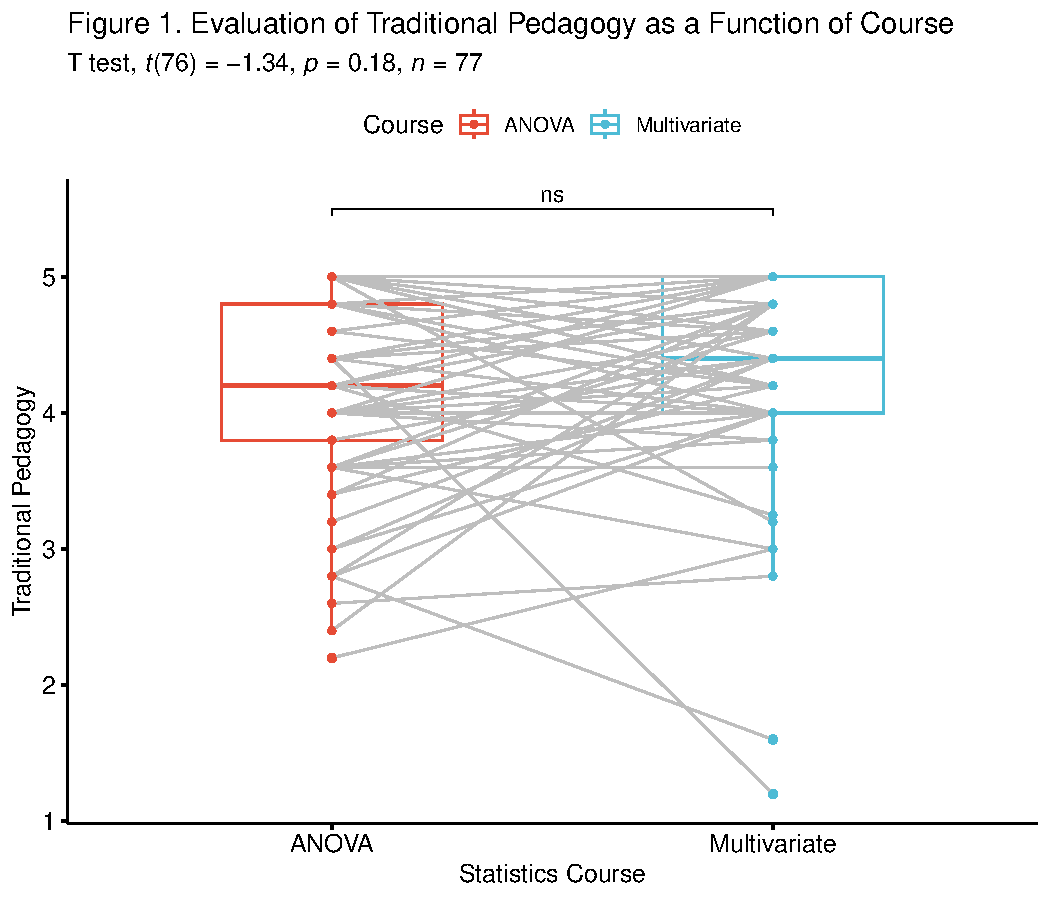
\includegraphics{06-tPairedSamples_files/figure-latex/unnamed-chunk-51-1.pdf}

\hypertarget{conduct-power-analyses-to-determine-the-power-of-the-current-study-and-a-recommended-sample-size-2}{%
\subsubsection{Conduct power analyses to determine the power of the current study and a recommended sample size}\label{conduct-power-analyses-to-determine-the-power-of-the-current-study-and-a-recommended-sample-size-2}}

Script for estimating current power:

\begin{itemize}
\tightlist
\item
  d is Cohen's \emph{d}
\item
  n is number of pairs, but set to NULL if we want to estimate sample size
\item
  power is conventionally set at .80, but left at NULL when we want to estimate power
\item
  sig.level is conventionlaly set at 0.05
\item
  type indicates the type of \emph{t}-test; in this example it is ``paired''
\item
  alternative indicates one or two.sided
\end{itemize}

\begin{Shaded}
\begin{Highlighting}[]
\NormalTok{pwr}\SpecialCharTok{::}\FunctionTok{pwr.t.test}\NormalTok{(}\AttributeTok{d =} \SpecialCharTok{{-}}\FloatTok{0.153}\NormalTok{, }\AttributeTok{n =} \DecValTok{77}\NormalTok{, }\AttributeTok{power =} \ConstantTok{NULL}\NormalTok{, }\AttributeTok{sig.level =} \FloatTok{0.05}\NormalTok{, }\AttributeTok{type =} \StringTok{"paired"}\NormalTok{,}
    \AttributeTok{alternative =} \StringTok{"two.sided"}\NormalTok{)}
\end{Highlighting}
\end{Shaded}

\begin{verbatim}

     Paired t test power calculation 

              n = 77
              d = 0.153
      sig.level = 0.05
          power = 0.2634404
    alternative = two.sided

NOTE: n is number of *pairs*
\end{verbatim}

We had a 26\% chance of finding a statistically significant result if, in fact, one existed.

\begin{Shaded}
\begin{Highlighting}[]
\NormalTok{pwr}\SpecialCharTok{::}\FunctionTok{pwr.t.test}\NormalTok{(}\AttributeTok{d =} \SpecialCharTok{{-}}\FloatTok{0.153}\NormalTok{, }\AttributeTok{n =} \ConstantTok{NULL}\NormalTok{, }\AttributeTok{power =} \FloatTok{0.8}\NormalTok{, }\AttributeTok{sig.level =} \FloatTok{0.05}\NormalTok{, }\AttributeTok{type =} \StringTok{"paired"}\NormalTok{,}
    \AttributeTok{alternative =} \StringTok{"two.sided"}\NormalTok{)}
\end{Highlighting}
\end{Shaded}

\begin{verbatim}

     Paired t test power calculation 

              n = 337.2182
              d = 0.153
      sig.level = 0.05
          power = 0.8
    alternative = two.sided

NOTE: n is number of *pairs*
\end{verbatim}

If we presumed power were at 80\%, we would need a sample size of 337.

\hypertarget{hand-calculations-3}{%
\subsection{Hand Calculations}\label{hand-calculations-3}}

For these hand calculations I will used the ``paired\_wide'' dataframe that we had prepared for the homework assignment intended for R and R packages.

\hypertarget{using-traditional-nhst-null-hypothesis-testing-language-state-your-null-and-alternative-hypotheses-2}{%
\subsubsection{Using traditional NHST (null hypothesis testing language), state your null and alternative hypotheses}\label{using-traditional-nhst-null-hypothesis-testing-language-state-your-null-and-alternative-hypotheses-2}}

The null hypotheses states that the true difference in means is zero. \(H_{O}: \mu _{D} = 0\)

The alternative hypothesis states that the true difference in means is not zero. \(H_{A}: \mu _{D}\neq 0\)

\hypertarget{using-an-r-package-or-functions-in-base-r-and-with-data-in-the-wide-format-calculate-the-difference-score-between-the-two-observations-of-the-dependent-variable}{%
\subsubsection{\texorpdfstring{Using an R package or functions in base R (and with data in the ``wide'' format), calculate the \emph{difference} score between the two observations of the dependent variable}{Using an R package or functions in base R (and with data in the ``wide'' format), calculate the difference score between the two observations of the dependent variable}}\label{using-an-r-package-or-functions-in-base-r-and-with-data-in-the-wide-format-calculate-the-difference-score-between-the-two-observations-of-the-dependent-variable}}

We had already calculated a difference score in the earlier assignment. Here it is again.

\begin{Shaded}
\begin{Highlighting}[]
\NormalTok{paired\_wide}\SpecialCharTok{$}\NormalTok{DIFF }\OtherTok{\textless{}{-}}\NormalTok{ paired\_wide}\SpecialCharTok{$}\NormalTok{ANOVA }\SpecialCharTok{{-}}\NormalTok{ paired\_wide}\SpecialCharTok{$}\NormalTok{Multivariate}
\end{Highlighting}
\end{Shaded}

\hypertarget{obtain-the-mean-and-standard-deviation-of-the-difference-score}{%
\subsubsection{\texorpdfstring{Obtain the mean and standard deviation of the \emph{difference} score}{Obtain the mean and standard deviation of the difference score}}\label{obtain-the-mean-and-standard-deviation-of-the-difference-score}}

We can obtain the mean and standard deviation for the difference score with this script.

\begin{Shaded}
\begin{Highlighting}[]
\NormalTok{psych}\SpecialCharTok{::}\FunctionTok{describe}\NormalTok{(paired\_wide}\SpecialCharTok{$}\NormalTok{DIFF)}
\end{Highlighting}
\end{Shaded}

\begin{verbatim}
   vars  n  mean  sd median trimmed  mad  min max range skew kurtosis   se
X1    1 77 -0.12 0.8   -0.2   -0.13 0.59 -2.4 3.2   5.6 0.56     3.15 0.09
\end{verbatim}

The mean difference (\(\bar{D}\)) is -0.12; the standard deviation (\(\hat\sigma_D\)) of the difference score is 0.8.

\hypertarget{calculate-the-paired-samples-t-test}{%
\subsubsection{\texorpdfstring{Calculate the paired samples \emph{t}-test}{Calculate the paired samples t-test}}\label{calculate-the-paired-samples-t-test}}

Here is the formula for the paired samples \emph{t}-test:

\[t = \frac{\bar{D}}{\hat\sigma_D / \sqrt{N}}\] Using the values we located we can calculate the value of the \emph{t} statistic.

\begin{Shaded}
\begin{Highlighting}[]
\SpecialCharTok{{-}}\FloatTok{0.12}\SpecialCharTok{/}\NormalTok{(}\FloatTok{0.8}\SpecialCharTok{/}\FunctionTok{sqrt}\NormalTok{(}\DecValTok{77}\NormalTok{))}
\end{Highlighting}
\end{Shaded}

\begin{verbatim}
[1] -1.316245
\end{verbatim}

The value we calculated with the \emph{rstatix::t\_test()} function was -1.34. Considering rounding error, I think we got it!

\hypertarget{identify-the-degrees-of-freedom-associated-with-your-paired-samples-t-test}{%
\subsubsection{\texorpdfstring{Identify the degrees of freedom associated with your paired samples \emph{t}-test}{Identify the degrees of freedom associated with your paired samples t-test}}\label{identify-the-degrees-of-freedom-associated-with-your-paired-samples-t-test}}

We have 77 pairs. The df for the paired samples \emph{t}-test is \(N - 1\). Therefore, df = 76.

\hypertarget{locate-the-test-critical-value-for-your-paired-samples-t-test}{%
\subsubsection{\texorpdfstring{Locate the test critical value for your paired samples \emph{t}-test}{Locate the test critical value for your paired samples t-test}}\label{locate-the-test-critical-value-for-your-paired-samples-t-test}}

I could look at the \href{https://www.statology.org/t-distribution-table/}{table of critical values} for the \emph{t}-distribution. Because I have non-directional hypotheses, I would use the column for a \emph{p}-value of .05 for a two-tailed test. I roll down to the closest sample size (I'll pick 60). This suggests that my \emph{t}-test statistic would need to be greater than 2.0 in order to be statistically significant.

I can also use the \emph{qt()} function in base R. This function requires that I specify the alpha level (0.05), whether the test is one- or two-tailed (2), and my degrees of freedom (76). Specifying ``TRUE'' and ``FALSE'' after the lower.tail command gives the positive and negative regions of rejection.

\begin{Shaded}
\begin{Highlighting}[]
\FunctionTok{qt}\NormalTok{(}\FloatTok{0.05}\SpecialCharTok{/}\DecValTok{2}\NormalTok{, }\DecValTok{76}\NormalTok{, }\AttributeTok{lower.tail =} \ConstantTok{TRUE}\NormalTok{)}
\end{Highlighting}
\end{Shaded}

\begin{verbatim}
[1] -1.991673
\end{verbatim}

\begin{Shaded}
\begin{Highlighting}[]
\FunctionTok{qt}\NormalTok{(}\FloatTok{0.05}\SpecialCharTok{/}\DecValTok{2}\NormalTok{, }\DecValTok{76}\NormalTok{, }\AttributeTok{lower.tail =} \ConstantTok{FALSE}\NormalTok{)}
\end{Highlighting}
\end{Shaded}

\begin{verbatim}
[1] 1.991673
\end{verbatim}

It is not surprising that these values are a smidge lower than 2.0. Why? Because in the table we stopped at df of 60, when it is actually 76.

\hypertarget{is-the-paired-samples-t-test-statistically-significant-why-or-why-not}{%
\subsubsection{\texorpdfstring{Is the paired samples \emph{t}-test statistically significant? Why or why not?}{Is the paired samples t-test statistically significant? Why or why not?}}\label{is-the-paired-samples-t-test-statistically-significant-why-or-why-not}}

The paired samples \emph{t}-test is not statistically significant because the \emph{t}-value of -1.316245 does not exceed -1.992.

\hypertarget{what-is-the-confidence-interval-around-the-mean-difference}{%
\subsubsection{What is the confidence interval around the mean difference?}\label{what-is-the-confidence-interval-around-the-mean-difference}}

Here is the formula for hand-calculating the confidence interval.

\[\bar{D}\pm t_{cv}(s_{d}/\sqrt{n})\]

\begin{itemize}
\tightlist
\item
  \(\bar{D}\) the mean difference score
\item
  \(t_{cv}\) the test critical value for a two-tailed model (even if the hypothesis was one-tailed) where \(\alpha = .05\) and the degrees of freedom are \(N-1\)
\item
  \(s_{d}\) the standard deviation of \(\bar{D}\)
\item
  \(N\) sample size
\end{itemize}

Let's calculate it:

\begin{Shaded}
\begin{Highlighting}[]
\SpecialCharTok{{-}}\FloatTok{0.12} \SpecialCharTok{{-}}\NormalTok{ (}\SpecialCharTok{{-}}\FloatTok{1.991673} \SpecialCharTok{*}\NormalTok{ ((}\FloatTok{0.8}\SpecialCharTok{/}\NormalTok{(}\FunctionTok{sqrt}\NormalTok{(}\DecValTok{77}\NormalTok{)))))}
\end{Highlighting}
\end{Shaded}

\begin{verbatim}
[1] 0.06157776
\end{verbatim}

\begin{Shaded}
\begin{Highlighting}[]
\SpecialCharTok{{-}}\FloatTok{0.12} \SpecialCharTok{+}\NormalTok{ (}\SpecialCharTok{{-}}\FloatTok{1.991673} \SpecialCharTok{*}\NormalTok{ ((}\FloatTok{0.8}\SpecialCharTok{/}\FunctionTok{sqrt}\NormalTok{(}\DecValTok{77}\NormalTok{))))}
\end{Highlighting}
\end{Shaded}

\begin{verbatim}
[1] -0.3015778
\end{verbatim}

These values indicate the range of scores in which we are 95\% confident that our true \(\bar{D}\) lies. Stated another way, we are 95\% confident that the true mean difference lies between -0.302 and 0.062. Because this interval crosses zero, we cannot rule out that the true mean difference is 0.00. This result is consistent with our non-significant \emph{p} value. For these types of statistics, the 95\% confidence interval and \emph{p} value will always be yoked together.

\hypertarget{calculate-the-effect-size-i.e.-cohens-d-associated-with-your-paired-samples-t-test}{%
\subsubsection{\texorpdfstring{Calculate the effect size (i.e., Cohen's \emph{d} associated with your paired samples \emph{t}-test}{Calculate the effect size (i.e., Cohen's d associated with your paired samples t-test}}\label{calculate-the-effect-size-i.e.-cohens-d-associated-with-your-paired-samples-t-test}}

Cohen's \emph{d} measures, in standard deviation units, the distance between the two means. Regardless of sign, values of .2, .5, and .8 are considered to be small, medium, and large, respectively.

Because the paired samples \emph{t}-test used the difference score in the numerator, there are two easy options for calculating this effect:

\[d=\frac{\bar{D}}{\hat\sigma_D}=\frac{t}{\sqrt{N}}\] Here's a demonstration of both:

\begin{Shaded}
\begin{Highlighting}[]
\SpecialCharTok{{-}}\FloatTok{0.12}\SpecialCharTok{/}\NormalTok{.}\DecValTok{8}
\end{Highlighting}
\end{Shaded}

\begin{verbatim}
[1] -0.15
\end{verbatim}

\begin{Shaded}
\begin{Highlighting}[]
\SpecialCharTok{{-}}\FloatTok{1.316245}\SpecialCharTok{/}\FunctionTok{sqrt}\NormalTok{(}\DecValTok{77}\NormalTok{)}
\end{Highlighting}
\end{Shaded}

\begin{verbatim}
[1] -0.15
\end{verbatim}

\hypertarget{assemble-the-results-into-a-statistical-string.}{%
\subsubsection{Assemble the results into a statistical string.}\label{assemble-the-results-into-a-statistical-string.}}

\(t(76) = -1.316, p > .05, CI95(-0.302, 0.062), d = -0.15\)

\hypertarget{analysis-of-variance}{%
\chapter*{Analysis of Variance}\label{analysis-of-variance}}


\hypertarget{oneway}{%
\chapter{One-way ANOVA}\label{oneway}}

\href{https://spu.hosted.panopto.com/Panopto/Pages/Viewer.aspx?pid=c88f8492-0599-462d-a471-ad8a01702156}{Screencasted Lecture Link}

One-way ANOVA allows the researcher to analyze mean differences between two or more groups on a between-subjects factor. For the one-way ANOVA, each case (i.e., individual, participant) must have scores on two variables: a factor and a dependent variable.

The factor must be categorical in nature, dividing the cases into two or more groups or levels. These levels could be ordered (e.g., placebo, low dose, high dose) or unordered (e.g., cognitive-behavioral, existential, psychodynamic). The dependent variable must be assessed on a quantitative, continuous dimension. The ANOVA \emph{F} test evaluates whether population means on the dependent variable differ across the levels of the factor.

One-way ANOVA can be used in experimental, quasi-experimental, and field studies. As we work through the chapter, we will examine some some of the requirements (assumptions) of the statistic in greater detail.

\hypertarget{navigating-this-lesson-5}{%
\section{Navigating this Lesson}\label{navigating-this-lesson-5}}

There is about 2 hours of lecture. If you work through the materials with me, plan for another two hours of study.

\hypertarget{learning-objectives-5}{%
\subsection{Learning Objectives}\label{learning-objectives-5}}

Learning objectives from this lecture include the following:

\begin{itemize}
\tightlist
\item
  Evaluate the statistical assumptions associated with one-way analysis of variance (ANOVA).
\item
  Describe the relationship between model/between-subjects and residual/within-subjects variance.
\item
  Narrate the steps in conducting a formal one-way ANOVA beginning with testing the statistical assumptions through writing up an APA style results section.
\item
  Conduct a one-way ANOVA in R (including calculation of effect sizes and follow-up to the omnibus).
\item
  Conduct a power analysis for a one-way ANOVA.
\item
  Produce an APA style results section for one-way ANOVA.
\end{itemize}

\hypertarget{planning-for-practice-4}{%
\subsection{Planning for Practice}\label{planning-for-practice-4}}

In each of these lessons I provide suggestions for practice that allow you to select one or more problems that are graded in difficulty. The least complex is to change the random seed and rework the problem demonstrated in the lesson. The results \emph{should} map onto the ones obtained in the lecture.

The second option comes from the research vignette. The Tran et al. \citeyearpar{tran_you_2014} vignette has two variables where the authors have conducted one-way ANOVAs. I will demonstrate one (\emph{Accurate}) in this lecture; the second is available as one of the homework options.

As a third option, you are welcome to use data to which you have access and is suitable for two-way ANOVA. In either case the practice options suggest that you:

\begin{itemize}
\tightlist
\item
  test the statistical assumptions
\item
  conduct a one-way ANOVA, including

  \begin{itemize}
  \tightlist
  \item
    omnibus test and effect size
  \item
    follow-up (pairwise, planned comparisons, polynomial trends)
  \end{itemize}
\item
  write a results section to include a figure and tables
\end{itemize}

\hypertarget{readings-resources-4}{%
\subsection{Readings \& Resources}\label{readings-resources-4}}

In preparing this chapter, I drew heavily from the following resource(s) that are freely available on the internet. Other resources are cited (when possible, linked) in the text with complete citations in the reference list.

\begin{itemize}
\tightlist
\item
  Crump, M. J. C. (2018). Chapter 5.5.2, Simulating data for one-way between subjects design with 3 levels. In \href{https://crumplab.github.io/programmingforpsych/simulating-and-analyzing-data-in-r.html\#single-factor-anovas-data-simulation-and-analysis}{Programming for Psychologists: Data Creation and Analysis}. Retrieved from \url{https://crumplab.github.io/programmingforpsych/simulating-and-analyzing-data-in-r.html\#single-factor-anovas-data-simulation-and-analysis}

  \begin{itemize}
  \tightlist
  \item
    Although this reference is on simulating data, the process of simulation can provide another perspective on one-way ANOVA.
  \end{itemize}
\item
  Kassambara, A. (n.d.). ANOVA in R: The Ultimate Guide. Datanovia. Retrieved December 28, 2022, from \url{https://www.datanovia.com/en/lessons/anova-in-r/}

  \begin{itemize}
  \tightlist
  \item
    In order to streamline the learning process, I have chosen to use \emph{rstatix} package for the majority of ANOVA lessons. There are a number of tutorials about this package as well as its integration with \emph{ggpubr} for creating relatively easy creation of attractive and informative figures. This tutorial is especially helpful.
  \end{itemize}
\item
  Navarro, D. (2020). Chapter 14: Comparing Several Means (one-Way ANOVA). In \href{https://learningstatisticswithr.com/}{Learning Statistics with R - A tutorial for Psychology Students and other Beginners}. Retrieved from \url{https://stats.libretexts.org/Bookshelves/Applied_Statistics/Book\%3A_Learning_Statistics_with_R_-_A_tutorial_for_Psychology_Students_and_other_Beginners_(Navarro)}

  \begin{itemize}
  \tightlist
  \item
    Navarro's OER includes a good mix of conceptual information about one-way ANOVA as well as R code. My code/approach is a mix of Green and Salkind's \citeyearpar{green_using_2017}, Field's \citeyearpar{field_discovering_2012}, Navarro's \citeyearpar{navarro_chapter_2020} chapters as well as other techniques I have found on the internet and learned from my students.
  \end{itemize}
\item
  Tran, A. G. T. T., \& Lee, R. M. (2014). You speak English well! Asian Americans' reactions to an exceptionalizing stereotype. \emph{Journal of Counseling Psychology, 61}(3), 484--490. \url{https://doi.org/10.1037/cou0000034}

  \begin{itemize}
  \tightlist
  \item
    The source of our research vignette.
  \end{itemize}
\end{itemize}

\hypertarget{packages-3}{%
\subsection{Packages}\label{packages-3}}

The packages used in this lesson are embedded in this code. When the hashtags are removed, the script below will (a) check to see if the following packages are installed on your computer and, if not (b) install them.

\begin{Shaded}
\begin{Highlighting}[]
\CommentTok{\# will install the package if not already installed \#easy plotting}
\CommentTok{\# for simple ANOVA if(!require(knitr))\{install.packages(\textquotesingle{}knitr\textquotesingle{})\}}
\CommentTok{\# \#not needed for conducting the statistics, but necessary for}
\CommentTok{\# knitting the document (if desired)}
\CommentTok{\# if(!require(tidyverse))\{install.packages(\textquotesingle{}tidyverse\textquotesingle{})\} \#a specific}
\CommentTok{\# part of the tidyverse with useful tools for manipulating data}
\CommentTok{\# if(!require(dplyr))\{install.packages(\textquotesingle{}dplyr\textquotesingle{})\} \#for descriptive}
\CommentTok{\# statistics and writing them as csv files}
\CommentTok{\# if(!require(psych))\{install.packages(\textquotesingle{}psych\textquotesingle{})\} \#a number of}
\CommentTok{\# wrappers for ANOVA models; today for evaluating the Shapiro}
\CommentTok{\# if(!require(ggpubr))\{install.packages(\textquotesingle{}ggpubr\textquotesingle{})\} \#the package we}
\CommentTok{\# will use to create figures}
\CommentTok{\# if(!require(rstatix))\{install.packages(\textquotesingle{}rstatix\textquotesingle{})\} \#the package we}
\CommentTok{\# will use for the majority of the ANOVA computations}
\CommentTok{\# if(!require(apaTAbles))\{install.packages(\textquotesingle{}apaTables\textquotesingle{})\} \#helps with}
\CommentTok{\# formats like decimals and percentages for inline code}
\CommentTok{\# if(!require(effectsize))\{install.packages(\textquotesingle{}effectsize\textquotesingle{})\}}
\CommentTok{\# if(!require(pwr))\{install.packages(\textquotesingle{}pwr\textquotesingle{})\} \#produces an APA style}
\CommentTok{\# table for ANOVAs and other models}
\CommentTok{\# if(!require(car))\{install.packages(\textquotesingle{}car\textquotesingle{})\}\#although we don\textquotesingle{}t call}
\CommentTok{\# this package directly, there are rstatix functions that are a}
\CommentTok{\# wrapper for it and therefore it needs to be installed}
\end{Highlighting}
\end{Shaded}

\hypertarget{workflow-for-one-way-anova}{%
\section{Workflow for One-Way ANOVA}\label{workflow-for-one-way-anova}}

The following is a proposed workflow for conducting a one-way ANOVA.

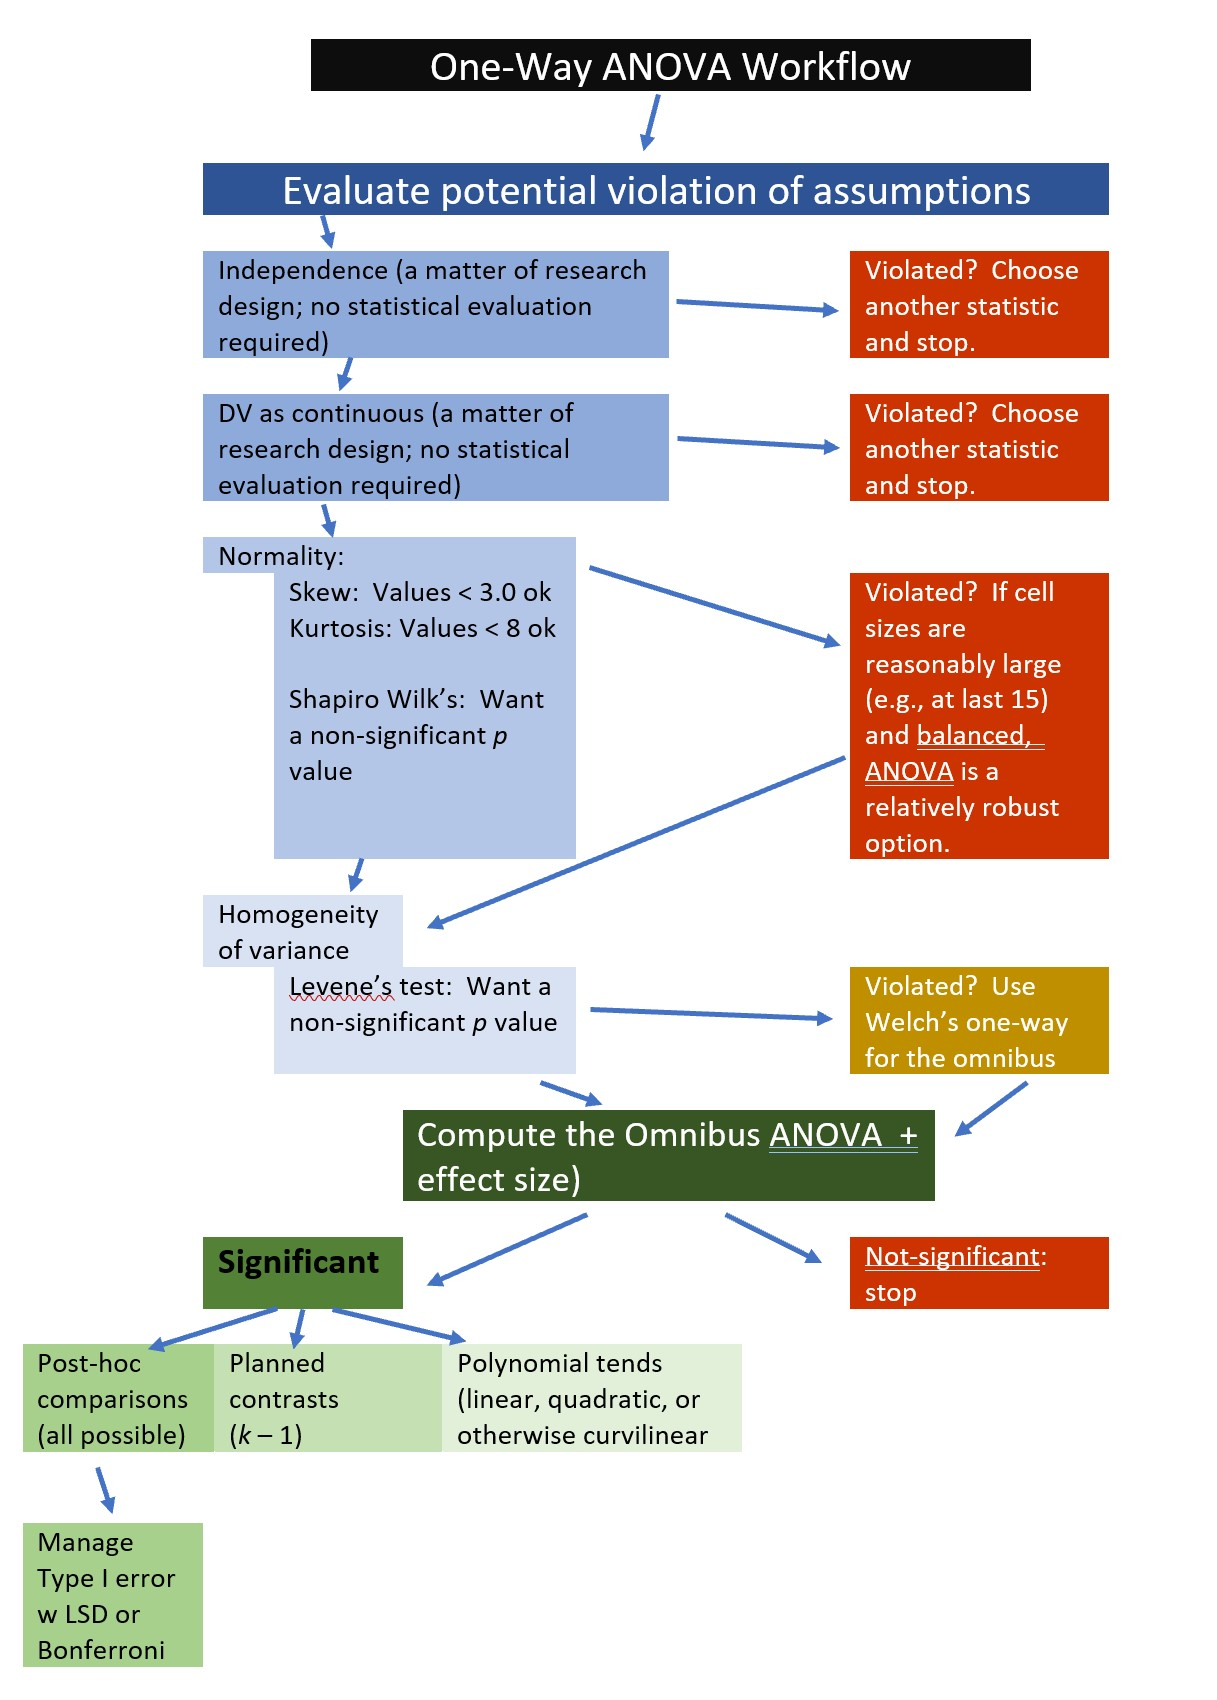
\includegraphics{images/oneway/OnewayWrkFlw.jpg} Utilizing one-way ANOVA involves the following steps:

\begin{enumerate}
\def\labelenumi{\arabic{enumi}.}
\tightlist
\item
  Prepare (upload) data.
\item
  Explore data

  \begin{itemize}
  \tightlist
  \item
    graphs
  \item
    descriptive statistics
  \end{itemize}
\item
  Checking distributional assumptions

  \begin{itemize}
  \tightlist
  \item
    assessing normality via skew, kurtosis, Shapiro-Wilks
  \item
    checking for violation of homogeneity of variance assumption with Levene's test; if we violate this we can use Welch's omnibus ANOVA
  \end{itemize}
\item
  Compute the omnibus ANOVA (remember to use Welch's if Levene's \emph{p} \textless{} .05)
\item
  Compute post hoc comparisons, planned contrasts, or polynomial trends
\item
  Managing Type I error
\item
  Sample size/power analysis (which you should think about first -- but in the context of teaching ANOVA, it's more pedagogically sensible, here)
\end{enumerate}

\hypertarget{research-vignette-4}{%
\section{Research Vignette}\label{research-vignette-4}}

The \emph{exceptionalizing racial stereotype} is microaggression framed as interpersonally complimentary, but perpetuates negative stereotypical views of a racial/ethnic group. We are using data that is simulated from a random clinical trial (RCT) conducted by Tran and Lee \citeyearpar{tran_you_2014}.

The one-way ANOVA examples we are simulating represent the post-only design which investigated three levels of the exceptionalizing stereotype in a sample of Asian American participants. This experimental design involved a confederate (posing as a peer) whose parting comment fell into the low racial loading, high racial loading, or control conditions.

\begin{longtable}[]{@{}
  >{\raggedright\arraybackslash}p{(\columnwidth - 6\tabcolsep) * \real{0.2388}}
  >{\raggedright\arraybackslash}p{(\columnwidth - 6\tabcolsep) * \real{0.1791}}
  >{\raggedright\arraybackslash}p{(\columnwidth - 6\tabcolsep) * \real{0.2687}}
  >{\raggedright\arraybackslash}p{(\columnwidth - 6\tabcolsep) * \real{0.3134}}@{}}
\toprule\noalign{}
\begin{minipage}[b]{\linewidth}\raggedright
COND
\end{minipage} & \begin{minipage}[b]{\linewidth}\raggedright
Assignment
\end{minipage} & \begin{minipage}[b]{\linewidth}\raggedright
Manipulation
\end{minipage} & \begin{minipage}[b]{\linewidth}\raggedright
Post-test Observation
\end{minipage} \\
\midrule\noalign{}
\endhead
\bottomrule\noalign{}
\endlastfoot
\textbf{Low} racial loading condition (\emph{n} = 22) & Random & Yes: ``Nice talking to you. You speak English well.'' & \textbf{Accurate} \\
\textbf{High} racial loading (\emph{n} = 23) & Random & Yes: ``Nice talking to you. You speak English well for an Asian.'' & \textbf{Accurate} \\
\textbf{Control} (\emph{n} = 23) & Random & No: ``Nice talking to you.'' & \textbf{Accurate} \\
\end{longtable}

In the article, the one-way ANOVA is a relatively smaller focus. In fact, Tran and Lee \citeyearpar{tran_you_2014} reported results from two ANOVAs and 4 ANCOVAs, using a pre-test as a covariate. A preprint of their article is available \href{https://pdfs.semanticscholar.org/4146/b528961c041de317c6a4c699f12fc5a4bc22.pdf?_ga=2.179078439.2028716028.1610939782-1660125104.1610939782}{here}. If you are interested in this topic, I highly encourage you to review the more complex analyses and their results.

\begin{itemize}
\tightlist
\item
  \textbf{Accurate} is the DV we will be exploring in this lesson. Participants rated how \emph{accurate} they believed their partner's impression of them was (0 = \emph{very inaccurate}, 3 = \emph{very accurate}).
\item
  \textbf{moreTalk} is the DV suggested as a practice problem. Participants rated how much longer they would continue the interaction with their partner compared to their interactions in general (-2 = \emph{much less than average}, 0 = \emph{average}, 2 = \emph{much more than average}).
\end{itemize}

\hypertarget{data-simulation-2}{%
\subsection{Data Simulation}\label{data-simulation-2}}

Simulating data for a one-way ANOVA requires the sample size (listed first), mean (mean=), and standard deviation (sd=) for each of the groups \citep{crump_simulating_2018}. In creating this simulation, I used the data from Table 1 in the Tran and Lee \citeyearpar{tran_you_2014} article. Having worked the problem several times, I made one change. The group sizes in the original study were 23, 22, and 23. To increase the probability that we would have statistically significant results in our worked example, I increased the sample sizes to 30 for each group. In this way we have a perfectly \emph{balanced} (equal cell sizes) design.

\begin{Shaded}
\begin{Highlighting}[]
\CommentTok{\# Note, this script results in a different simulation than is in the}
\CommentTok{\# ReadySetR lesson sets a random seed so that we get the same results}
\CommentTok{\# each time}
\FunctionTok{set.seed}\NormalTok{(}\DecValTok{210820}\NormalTok{)}
\CommentTok{\# sample size, M and SD for each group}
\NormalTok{Accurate }\OtherTok{\textless{}{-}} \FunctionTok{c}\NormalTok{(}\FunctionTok{rnorm}\NormalTok{(}\DecValTok{30}\NormalTok{, }\AttributeTok{mean =} \FloatTok{1.18}\NormalTok{, }\AttributeTok{sd =} \FloatTok{0.8}\NormalTok{), }\FunctionTok{rnorm}\NormalTok{(}\DecValTok{30}\NormalTok{, }\AttributeTok{mean =} \FloatTok{1.83}\NormalTok{,}
    \AttributeTok{sd =} \FloatTok{0.58}\NormalTok{), }\FunctionTok{rnorm}\NormalTok{(}\DecValTok{30}\NormalTok{, }\AttributeTok{mean =} \FloatTok{1.76}\NormalTok{, }\AttributeTok{sd =} \FloatTok{0.56}\NormalTok{))}
\CommentTok{\# set upper bound for DV}
\NormalTok{Accurate[Accurate }\SpecialCharTok{\textgreater{}} \DecValTok{3}\NormalTok{] }\OtherTok{\textless{}{-}} \DecValTok{3}
\CommentTok{\# set lower bound for DV}
\NormalTok{Accurate[Accurate }\SpecialCharTok{\textless{}} \DecValTok{0}\NormalTok{] }\OtherTok{\textless{}{-}} \DecValTok{0}
\CommentTok{\# sample size, M and SD for each group}
\NormalTok{moreTalk }\OtherTok{\textless{}{-}} \FunctionTok{c}\NormalTok{(}\FunctionTok{rnorm}\NormalTok{(}\DecValTok{30}\NormalTok{, }\AttributeTok{mean =} \SpecialCharTok{{-}}\FloatTok{0.82}\NormalTok{, }\AttributeTok{sd =} \FloatTok{0.91}\NormalTok{), }\FunctionTok{rnorm}\NormalTok{(}\DecValTok{30}\NormalTok{, }\AttributeTok{mean =} \SpecialCharTok{{-}}\FloatTok{0.39}\NormalTok{,}
    \AttributeTok{sd =} \FloatTok{0.66}\NormalTok{), }\FunctionTok{rnorm}\NormalTok{(}\DecValTok{30}\NormalTok{, }\AttributeTok{mean =} \SpecialCharTok{{-}}\FloatTok{0.04}\NormalTok{, }\AttributeTok{sd =} \FloatTok{0.71}\NormalTok{))}
\CommentTok{\# set upper bound for DV}
\NormalTok{moreTalk[moreTalk }\SpecialCharTok{\textgreater{}} \DecValTok{2}\NormalTok{] }\OtherTok{\textless{}{-}} \DecValTok{2}
\CommentTok{\# set lower bound for DV}
\NormalTok{moreTalk[moreTalk }\OtherTok{\textless{}{-}} \DecValTok{2}\NormalTok{] }\OtherTok{\textless{}{-}} \SpecialCharTok{{-}}\DecValTok{2}
\CommentTok{\# IDs for participants}
\NormalTok{ID }\OtherTok{\textless{}{-}} \FunctionTok{factor}\NormalTok{(}\FunctionTok{seq}\NormalTok{(}\DecValTok{1}\NormalTok{, }\DecValTok{90}\NormalTok{))}
\CommentTok{\# name factors and identify how many in each group; should be in same}
\CommentTok{\# order as first row of script}
\NormalTok{COND }\OtherTok{\textless{}{-}} \FunctionTok{c}\NormalTok{(}\FunctionTok{rep}\NormalTok{(}\StringTok{"High"}\NormalTok{, }\DecValTok{30}\NormalTok{), }\FunctionTok{rep}\NormalTok{(}\StringTok{"Low"}\NormalTok{, }\DecValTok{30}\NormalTok{), }\FunctionTok{rep}\NormalTok{(}\StringTok{"Control"}\NormalTok{, }\DecValTok{30}\NormalTok{))}
\CommentTok{\# groups the 3 variables into a single df: ID\#, DV, condition}
\NormalTok{accSIM30 }\OtherTok{\textless{}{-}} \FunctionTok{data.frame}\NormalTok{(ID, COND, Accurate, moreTalk)}
\end{Highlighting}
\end{Shaded}

Examining the data is important for several reasons. First, we can begin our inspection for anomalies. Second, if we are confused about what statistic we wish to apply, understanding the characteristics of the data can provide clues.

We can see the entire dataframe by clicking open the dataframe object found in the Environment window of R studio. This will open a tab that allows scrolling up/down and left/right through the entire dataframe. It is also possible to sort by variables.

Alternatively the \emph{head()} function from base R displays a static view of the first six rows of data.

\begin{Shaded}
\begin{Highlighting}[]
\FunctionTok{head}\NormalTok{(accSIM30)}
\end{Highlighting}
\end{Shaded}

\begin{verbatim}
  ID COND  Accurate   moreTalk
1  1 High 0.4203896 -0.6398265
2  2 High 1.1226505 -2.0000000
3  3 High 0.8852238 -0.2497750
4  4 High 1.5689439  0.1455637
5  5 High 1.8307196 -0.9960413
6  6 High 1.8874431 -1.0692978
\end{verbatim}

Yet another option is to use the \emph{str()} function from base R. This provides a list of variables and provides detail about their formats.

\begin{Shaded}
\begin{Highlighting}[]
\FunctionTok{str}\NormalTok{(accSIM30)}
\end{Highlighting}
\end{Shaded}

\begin{verbatim}
'data.frame':   90 obs. of  4 variables:
 $ ID      : Factor w/ 90 levels "1","2","3","4",..: 1 2 3 4 5 6 7 8 9 10 ...
 $ COND    : chr  "High" "High" "High" "High" ...
 $ Accurate: num  0.42 1.123 0.885 1.569 1.831 ...
 $ moreTalk: num  -0.64 -2 -0.25 0.146 -0.996 ...
\end{verbatim}

If we look at this simple dataset, we see that we see that

\begin{itemize}
\tightlist
\item
  \textbf{COND} is a grouping variable) with 3 levels (high, low, control)

  \begin{itemize}
  \tightlist
  \item
    it is presently in ``chr'' (character) format, it needs to be changed to be a factor.
  \end{itemize}
\item
  \textbf{Accurate} is a continuous variable

  \begin{itemize}
  \tightlist
  \item
    it is presently in ``num'' (numerical) format, this is an appropriate format.
  \end{itemize}
\item
  \textbf{moreTalk} is a continuous variable

  \begin{itemize}
  \tightlist
  \item
    it is presently in ``num'' (numerical) format, this is an appropriate format
  \end{itemize}
\end{itemize}

There are many ways to convert variables to factors; here is one of the simplest.

\begin{Shaded}
\begin{Highlighting}[]
\CommentTok{\#convert variable to factor}
\NormalTok{accSIM30}\SpecialCharTok{$}\NormalTok{COND }\OtherTok{\textless{}{-}} \FunctionTok{factor}\NormalTok{(accSIM30}\SpecialCharTok{$}\NormalTok{COND)}
\end{Highlighting}
\end{Shaded}

Let's recheck the structure

\begin{Shaded}
\begin{Highlighting}[]
\FunctionTok{str}\NormalTok{(accSIM30)}
\end{Highlighting}
\end{Shaded}

\begin{verbatim}
'data.frame':   90 obs. of  4 variables:
 $ ID      : Factor w/ 90 levels "1","2","3","4",..: 1 2 3 4 5 6 7 8 9 10 ...
 $ COND    : Factor w/ 3 levels "Control","High",..: 2 2 2 2 2 2 2 2 2 2 ...
 $ Accurate: num  0.42 1.123 0.885 1.569 1.831 ...
 $ moreTalk: num  -0.64 -2 -0.25 0.146 -0.996 ...
\end{verbatim}

By default, R orders factors alphabetically. This means, analyses will assume that ``Control'' (C) is the lowest condition, then ``High,'' then ``Low.'' Since these have theoretically ordered values, we want them in the order of ``Control,'' ``Low,'' ``High.''

Here is the script to create an ordered factor. The order in which the variables are entered in the concatenated list (``c'') establishes the order (e.g., levels).

\begin{Shaded}
\begin{Highlighting}[]
\CommentTok{\# ordering the factor}
\NormalTok{accSIM30}\SpecialCharTok{$}\NormalTok{COND }\OtherTok{\textless{}{-}} \FunctionTok{factor}\NormalTok{(accSIM30}\SpecialCharTok{$}\NormalTok{COND, }\AttributeTok{levels =} \FunctionTok{c}\NormalTok{(}\StringTok{"Control"}\NormalTok{, }\StringTok{"Low"}\NormalTok{, }\StringTok{"High"}\NormalTok{))}
\end{Highlighting}
\end{Shaded}

Again, we can check our work.

\begin{Shaded}
\begin{Highlighting}[]
\CommentTok{\#another structure check}
\FunctionTok{str}\NormalTok{(accSIM30)}
\end{Highlighting}
\end{Shaded}

\begin{verbatim}
'data.frame':   90 obs. of  4 variables:
 $ ID      : Factor w/ 90 levels "1","2","3","4",..: 1 2 3 4 5 6 7 8 9 10 ...
 $ COND    : Factor w/ 3 levels "Control","Low",..: 3 3 3 3 3 3 3 3 3 3 ...
 $ Accurate: num  0.42 1.123 0.885 1.569 1.831 ...
 $ moreTalk: num  -0.64 -2 -0.25 0.146 -0.996 ...
\end{verbatim}

Now our variables are suitable for analysis.

Although you may continue working with the simulated data, at this point, you may wish to export and/or import the data as a .csv (think ``Excel lite'') or .rds (R object that preserves the information about the variables -- such changing COND to an ordered factor). Here is the code to do so. The data should save in the same folder as the .rmd file. Therefore, it is really important (think, ``good R hygiene'') to have organized your folders so that your .rmd and data files are co-located.

I have hashtagged out the code. If you wish to use it, delete the hashtags. Although I show the .csv code first, my personal preference is to save R data as .rds files. While they aren't easy to ``see'' as an independent file, they retain the formatting of the variables. For a demonstration, refer back to the \protect\hyperlink{Ready}{Ready\_Set\_R} lesson.

\begin{Shaded}
\begin{Highlighting}[]
\CommentTok{\# write the simulated data as a .csv write.table(accSIM30,}
\CommentTok{\# file=\textquotesingle{}accSIM.csv\textquotesingle{}, sep=\textquotesingle{},\textquotesingle{}, col.names=TRUE, row.names=FALSE) bring}
\CommentTok{\# back the simulated dat from a .csv file acc\_csv \textless{}{-}}
\CommentTok{\# read.csv(\textquotesingle{}accSIM.csv\textquotesingle{}, header = TRUE)}
\end{Highlighting}
\end{Shaded}

If you have cleared the environment and then imported the .csv file, examining the structure of the .csv file shows that the prior formatting is lost. This is demonstrated in the accompanying screencast.

\begin{Shaded}
\begin{Highlighting}[]
\CommentTok{\# a quick demo to show that the .csv format loses the variable}
\CommentTok{\# formatting str(acc\_csv)}
\end{Highlighting}
\end{Shaded}

Below is the code to write and then import the data as an .rds file.

\begin{Shaded}
\begin{Highlighting}[]
\CommentTok{\# to save the df as an .rds (think \textquotesingle{}R object\textquotesingle{}) file on your computer;}
\CommentTok{\# it should save in the same file as the .rmd file you are working}
\CommentTok{\# with saveRDS(accSIM30, \textquotesingle{}accSIM.rds\textquotesingle{}) bring back the simulated dat}
\CommentTok{\# from an .rds file acc\_RDS \textless{}{-} readRDS(\textquotesingle{}accSIM.rds\textquotesingle{})}
\end{Highlighting}
\end{Shaded}

By examining the structure of the .rds file we can see that the .rds file preserves the variable formatting. This is demonstrated in the accompanying screencast.

\begin{Shaded}
\begin{Highlighting}[]
\CommentTok{\# a quick demo to show that the .rds format preserves the variable}
\CommentTok{\# formatting str(acc\_RDS)}
\end{Highlighting}
\end{Shaded}

Note that I renamed each of these data objects to reflect the form in whic I saved them (i.e., ``acc\_csv'', ``acc\_RDS''). If you have followed this step, you will want to rename the file before continuing with the rest of the chapter. Alternatively, you can start from scratch, re-run the code to simulate the data, and skip this portion on importing/exporting data.

\begin{Shaded}
\begin{Highlighting}[]
\CommentTok{\#accSIM30 \textless{}{-} acc\_RDS}
\CommentTok{\#or}
\CommentTok{\#accSIM30 \textless{}{-} acc\_csv}
\end{Highlighting}
\end{Shaded}

\hypertarget{quick-peek-at-the-data-3}{%
\subsection{Quick Peek at the Data}\label{quick-peek-at-the-data-3}}

This lesson's exploration of the data is designed to introduce multiple tools for doing so. In this first demonstration I will quickly produce a mean and standard deviation using functions from base R.

The \emph{aggregate()} function lets R know we want output by a grouping variable. We then list the variable of interest, a tilda (I think of the word ``by''), and then the grouping variable (I think ``Accurate by COND''). Finally we list the dataframe and the statistic (e.g., mean or standard deviation). R is case sensitive -- so check your capitalization if your code fails to execute.

\begin{Shaded}
\begin{Highlighting}[]
\FunctionTok{aggregate}\NormalTok{(Accurate }\SpecialCharTok{\textasciitilde{}}\NormalTok{ COND, accSIM30, mean)}
\end{Highlighting}
\end{Shaded}

\begin{verbatim}
     COND Accurate
1 Control 1.756195
2     Low 1.900116
3    High 1.152815
\end{verbatim}

\begin{Shaded}
\begin{Highlighting}[]
\FunctionTok{aggregate}\NormalTok{(Accurate }\SpecialCharTok{\textasciitilde{}}\NormalTok{ COND, accSIM30, sd)}
\end{Highlighting}
\end{Shaded}

\begin{verbatim}
     COND  Accurate
1 Control 0.4603964
2     Low 0.6301138
3    High 0.6587486
\end{verbatim}

Inspection of the means and standard deviations shows that the racially loaded \emph{high} condition has the lowest accuracy score (\(M = 1.153\)) and the largest variability (\(SD = 0.659\)).

Graphing data is a best practice for early exploration and inspection of the data. In ANOVA models the boxplot is especially useful. The \emph{ggpubr} package offers terrific options. After calling \emph{ggpubr::ggboxplot()}, we list the data frame and name the x and y variables. That would be sufficient to produce a simple boxplot. The ``add = jitter'' command will plot each individual case, but ``jitter'' them to the right and left such that they are not overlapping and we can see all scores. For fun I added some color.

\begin{Shaded}
\begin{Highlighting}[]
\NormalTok{ggpubr}\SpecialCharTok{::}\FunctionTok{ggboxplot}\NormalTok{(accSIM30, }\AttributeTok{x =} \StringTok{"COND"}\NormalTok{, }\AttributeTok{y =} \StringTok{"Accurate"}\NormalTok{, }\AttributeTok{add =} \StringTok{"jitter"}\NormalTok{,}
    \AttributeTok{color =} \StringTok{"COND"}\NormalTok{, )}
\end{Highlighting}
\end{Shaded}

\includegraphics{07-OnewayANOVA_files/figure-latex/unnamed-chunk-15-1.pdf} In boxplots the center value is the median. The box spans the \emph{interquartile range} and ranges from the 25th to the 75th percentile. The whiskers cover 1.5 times the interquartile range. When this does not capture the entire range, outliers are represented with dots.

From both the boxplot and the linegraph with error bars, we can see that participants in the low racial loading condition have the highest accuracy ratings. This is followed by the control and then high racial loading conditions. Are these differences statistically significant? This is why we need the one-way ANOVA.

\hypertarget{working-the-oneway-anova-by-hand}{%
\section{Working the Oneway ANOVA (by hand)}\label{working-the-oneway-anova-by-hand}}

ANOVA was developed by Sir Ronald Fisher in the early 20th century. The name is a bit of a misnomer -- rather than analyzing \emph{variances}, we are investigating differences in \emph{means} (but the formula does take variances into consideration\ldots stay tuned).

ANOVA falls squarely within the tradition of \textbf{null hypothesis significance testing} (NHST). As such, a formal, traditional, ANOVA begins with statements of the null and alternate hypotheses. \emph{Note. In their article, Tran and Lee \citeyearpar{tran_you_2014} do not list such. This is farly common in present-day journal articles.}

In our example, we would hypothesize that the population means (i.e., Asian or Asian American individuals in the U.S.) are equal: \[H_{O}: \mu _{1} = \mu _{2} = \mu _{3}\] There are an number of ways that the \(H_{O}\) could be false. Here are a few: \[H_{a1}: \mu _{1} \neq \mu _{2} \neq \mu _{3}\] \[H_{a2}: \mu _{1} = \mu _{2} > \mu _{3}\] \[H_{a3}: \mu _{1} > \mu _{2} > \mu _{3}\] The bottom line is that if we have a statistically significant omnibus ANOVA (i.e., the test of the overall significance of the model) and the \(H_{O}\) is false, somewhere between the three levels of the grouping factor, the means are statistically significantly different from each other.

In evaluating the differences between means, one-way ANOVA compares:

\begin{itemize}
\tightlist
\item
  systematic variance to unsystematic variance
\item
  explained to unexplained variation
\item
  experimental effect to the individual differences
\item
  model variance to residual variance
\item
  between group variance to within group variance
\end{itemize}

The ratio of these variances is the \emph{F}-ratio.

Navarro \citeyearpar{navarro_book_2020} offers a set of useful figures to compare between- and within-group variation.

\begin{figure}
\centering
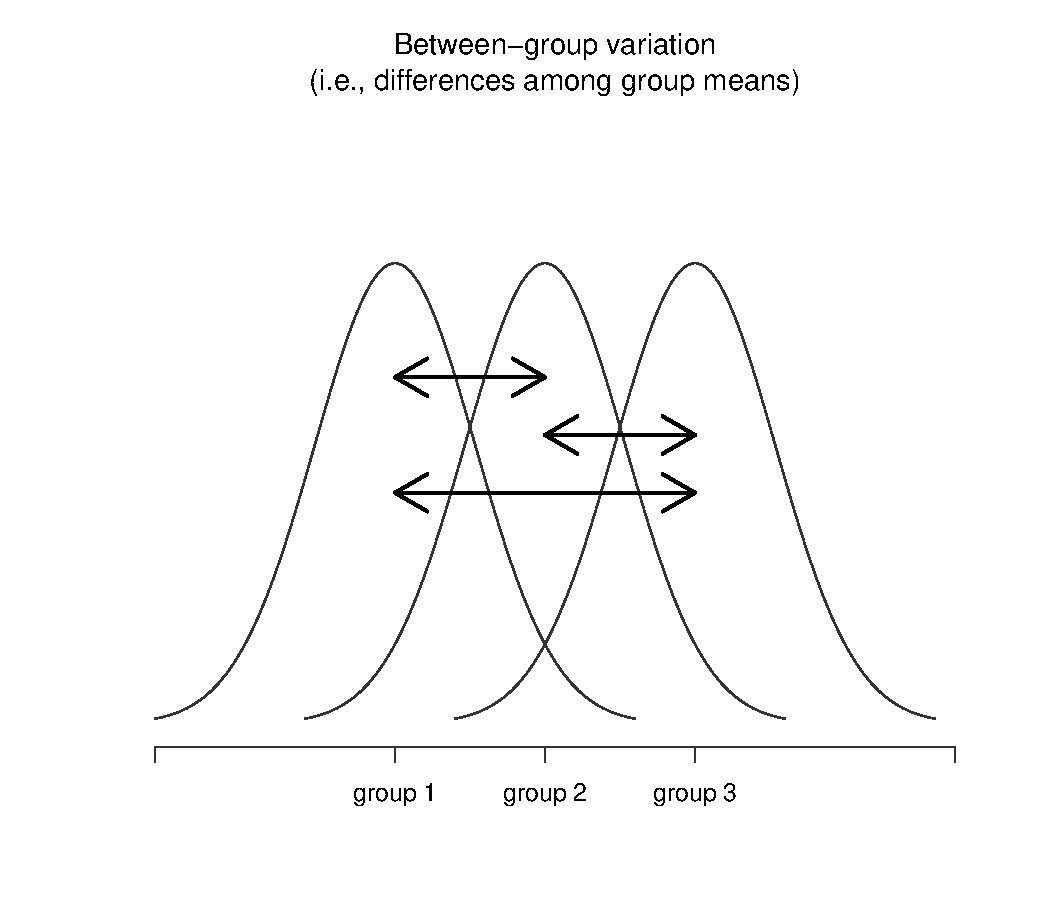
\includegraphics{07-OnewayANOVA_files/figure-latex/unnamed-chunk-16-1.pdf}
\caption{\label{fig:unnamed-chunk-16}Graphical illustration of ``between groups'' variation}
\end{figure}

\begin{figure}
\centering
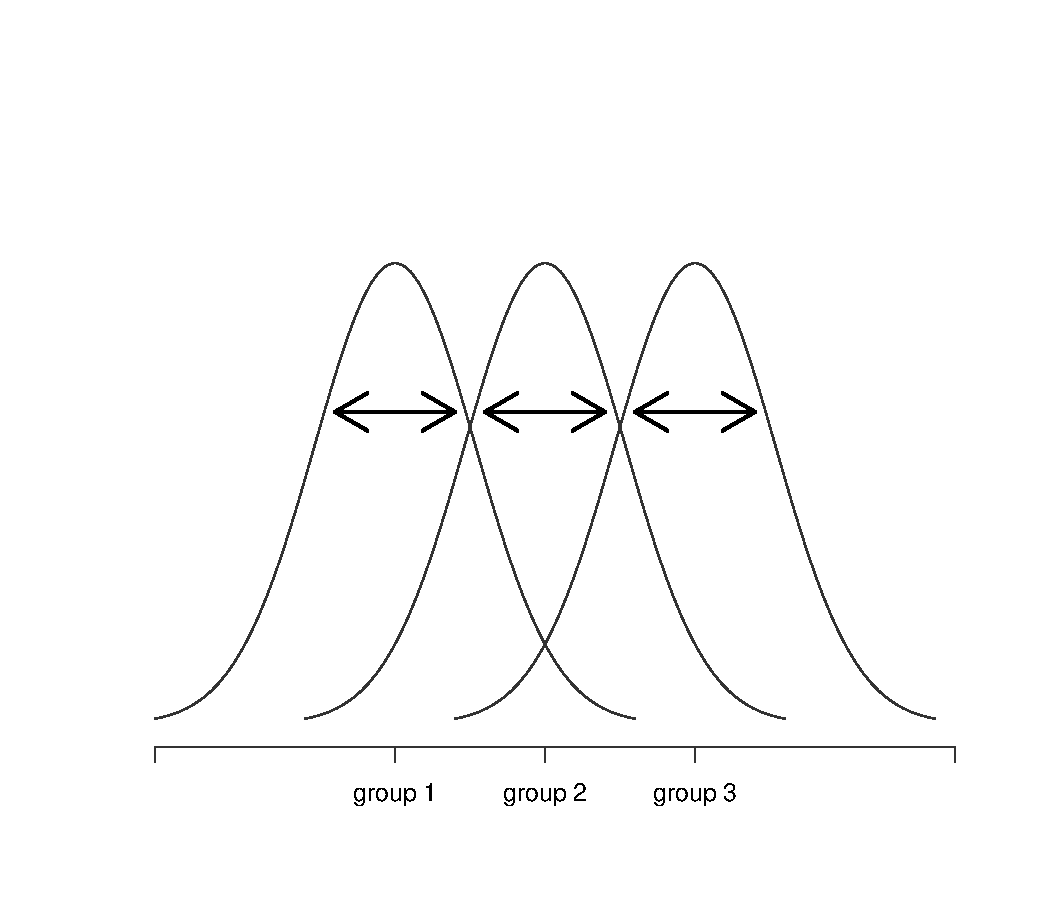
\includegraphics{07-OnewayANOVA_files/figure-latex/unnamed-chunk-17-1.pdf}
\caption{\label{fig:unnamed-chunk-17}Graphical illustration of ``within groups'' variation}
\end{figure}

When between-group variance (i.e,. model variance) is greater than within-group variance (i.e., residual variance) there may be support to suggest that there are statistically significant differences between groups.

Let's examine how variance is partitioned by hand-calculating sums of squares total, model, and residual. Along the way we will use some basic R skills to manipulate the data.

\hypertarget{sums-of-squares-total}{%
\subsection{Sums of Squares Total}\label{sums-of-squares-total}}

Sums of squares total represents the total amount of variance within our data. Examining the formula(s; there are variants of each) can help us gain a conceptual understanding of this.

In this first version of the formula we can see that the grand (or overall) mean is subtracted from each individual score, squared, and then summed. This makes sense: \emph{sums of squares, total}.

\[SS_{T}= \sum (x_{i}-\bar{x}_{grand})^{2}\] In the next version of the formula we see that the sums of square total is the addition of the sums of squares model and residual.

\[SS_{T}= SS_{M} + SS_{R}\]

``Between'' and ``within'' are another way to understand ``model'' and ``residual.'' This is reflected in the next formula.

\[SS_{T}= SS_{B} + SS_{W}\] Finally, think of the sums of squares total as the grand variance multiplied by the overall degrees of freedom (\emph{N} - 1).

\[SS_{T}= s_{grand}^{2}(n-1)\] Let's take a moment to \emph{hand-calculate} \(SS_{T}\). Not to worry -- we'll get R to do the math for us!

Our grand (i.e., overall) mean is

\begin{Shaded}
\begin{Highlighting}[]
\NormalTok{GrandMean }\OtherTok{\textless{}{-}} \FunctionTok{mean}\NormalTok{(accSIM30}\SpecialCharTok{$}\NormalTok{Accurate)}
\NormalTok{GrandMean}
\end{Highlighting}
\end{Shaded}

\begin{verbatim}
[1] 1.603042
\end{verbatim}

Subtracting the grand mean from each Accurate rating yields a mean difference. In the script below I have used the \emph{mutate()} function from the \emph{dplyr} package (a part of the \emph{tidyverse}) to created a new variable ('' m\_dev'') in the dataframe. The \emph{tidyverse} package is one of the few exceptions that I will open via the library. This is because we need it if we are going to use the pipe (\%\textgreater\%) to string parts of our script together.

\begin{Shaded}
\begin{Highlighting}[]
\FunctionTok{library}\NormalTok{(tidyverse)}

\NormalTok{accSIM30 }\OtherTok{\textless{}{-}}\NormalTok{ accSIM30 }\SpecialCharTok{\%\textgreater{}\%} 
\NormalTok{  dplyr}\SpecialCharTok{::}\FunctionTok{mutate}\NormalTok{(}\AttributeTok{m\_dev =}\NormalTok{ Accurate}\SpecialCharTok{{-}}\FunctionTok{mean}\NormalTok{(Accurate))}

\FunctionTok{head}\NormalTok{(accSIM30)}
\end{Highlighting}
\end{Shaded}

\begin{verbatim}
  ID COND  Accurate   moreTalk       m_dev
1  1 High 0.4203896 -0.6398265 -1.18265259
2  2 High 1.1226505 -2.0000000 -0.48039170
3  3 High 0.8852238 -0.2497750 -0.71781837
4  4 High 1.5689439  0.1455637 -0.03409829
5  5 High 1.8307196 -0.9960413  0.22767748
6  6 High 1.8874431 -1.0692978  0.28440098
\end{verbatim}

Pop quiz: What's the sum of our new \emph{m\_dev} variable? Let's check.

\begin{Shaded}
\begin{Highlighting}[]
\FunctionTok{mean}\NormalTok{(accSIM30}\SpecialCharTok{$}\NormalTok{m\_dev)}
\end{Highlighting}
\end{Shaded}

\begin{verbatim}
[1] 0.00000000000000003830065
\end{verbatim}

Unless you run the script at the top of this document (``options(scipen=999)''), R will (seemingly selectively) use \textbf{scientific e notation} to report your results. The proper value is one where the base number (before the ``e'') is multiplied by 10, raised to the power shown: \(3.830065 * 10^{17}\) Another way to think of it is to move the decimal 17 places to the left. In any case, this number is essentially zero.

Back to the point of sums of squares total, the sum of deviations around the grand mean will always be zero. To make them useful, we must square them:

\begin{Shaded}
\begin{Highlighting}[]
\NormalTok{accSIM30 }\OtherTok{\textless{}{-}}\NormalTok{ accSIM30 }\SpecialCharTok{\%\textgreater{}\%} 
\NormalTok{  dplyr}\SpecialCharTok{::}\FunctionTok{mutate}\NormalTok{(}\AttributeTok{m\_devSQ =}\NormalTok{ m\_dev}\SpecialCharTok{\^{}}\DecValTok{2}\NormalTok{)}

\FunctionTok{head}\NormalTok{(accSIM30)}
\end{Highlighting}
\end{Shaded}

\begin{verbatim}
  ID COND  Accurate   moreTalk       m_dev     m_devSQ
1  1 High 0.4203896 -0.6398265 -1.18265259 1.398667144
2  2 High 1.1226505 -2.0000000 -0.48039170 0.230776185
3  3 High 0.8852238 -0.2497750 -0.71781837 0.515263216
4  4 High 1.5689439  0.1455637 -0.03409829 0.001162694
5  5 High 1.8307196 -0.9960413  0.22767748 0.051837034
6  6 High 1.8874431 -1.0692978  0.28440098 0.080883915
\end{verbatim}

If we sum the squared mean deviations we will obtain the total variance (sums of squares total):

\begin{Shaded}
\begin{Highlighting}[]
\NormalTok{SST }\OtherTok{\textless{}{-}} \FunctionTok{sum}\NormalTok{(accSIM30}\SpecialCharTok{$}\NormalTok{m\_devSQ)}
\NormalTok{SST}
\end{Highlighting}
\end{Shaded}

\begin{verbatim}
[1] 39.67818
\end{verbatim}

This value, the sum of squared deviations around the grand mean, is our \(SS_T\). The associated \emph{degrees of freedom} is \(N - 1\); in our case this is 90-1 = 89.

In one-way ANOVA, we divide \(SS_T\) into \textbf{model/between sums of squares} and \textbf{residual/within sums of squares}.

The \emph{model} generally represents the notion that the means are different than each other. We want the variation between our means to be greater than the variation within each of the groups from which our means are calculated.

\hypertarget{sums-of-squares-for-the-model-or-between}{%
\subsection{Sums of Squares for the Model (or Between)}\label{sums-of-squares-for-the-model-or-between}}

We just determined that the total amount of variation within the data is 39.678 units. From this we can estimate how much of this variation our model can explain. \(SS_M\) tells us how much of the total variation can be explained by the fact that different data points come from different groups.

We see this reflected in the formula below, where

\begin{itemize}
\tightlist
\item
  the grand mean is subtracted from each group mean
\item
  this value is squared and multiplied by the number of cases in each group
\item
  these values are summed
\end{itemize}

\[SS_{M}= \sum n_{k}(\bar{x}_{k}-\bar{x}_{grand})^{2}\]

To calculate this, we start with the grand mean (previously calculated): 1.603.

We also estimate the group means. The script below provides the formula, the dataset, and the particular statistic (mean) that we want calculated.

\begin{Shaded}
\begin{Highlighting}[]
\NormalTok{GroupMeans }\OtherTok{\textless{}{-}} \FunctionTok{aggregate}\NormalTok{(Accurate }\SpecialCharTok{\textasciitilde{}}\NormalTok{ COND, accSIM30, mean)}
\NormalTok{GroupMeans}
\end{Highlighting}
\end{Shaded}

\begin{verbatim}
     COND Accurate
1 Control 1.756195
2     Low 1.900116
3    High 1.152815
\end{verbatim}

This script is used to extract the specific means so that I can demonstrate the formulas with the words/terms as well as the numbers.

\begin{Shaded}
\begin{Highlighting}[]
\NormalTok{ControlMean }\OtherTok{\textless{}{-}}\NormalTok{ (GroupMeans}\SpecialCharTok{$}\NormalTok{Accurate[}\DecValTok{1}\NormalTok{])}
\NormalTok{ControlMean}
\end{Highlighting}
\end{Shaded}

\begin{verbatim}
[1] 1.756195
\end{verbatim}

\begin{Shaded}
\begin{Highlighting}[]
\NormalTok{LowMean }\OtherTok{\textless{}{-}}\NormalTok{ (GroupMeans}\SpecialCharTok{$}\NormalTok{Accurate[}\DecValTok{2}\NormalTok{])}
\NormalTok{LowMean}
\end{Highlighting}
\end{Shaded}

\begin{verbatim}
[1] 1.900116
\end{verbatim}

\begin{Shaded}
\begin{Highlighting}[]
\NormalTok{HighMean }\OtherTok{\textless{}{-}}\NormalTok{ (GroupMeans}\SpecialCharTok{$}\NormalTok{Accurate[}\DecValTok{3}\NormalTok{])}
\NormalTok{HighMean}
\end{Highlighting}
\end{Shaded}

\begin{verbatim}
[1] 1.152815
\end{verbatim}

\begin{Shaded}
\begin{Highlighting}[]
\NormalTok{nGroup }\OtherTok{\textless{}{-}}\NormalTok{ accSIM30 }\SpecialCharTok{\%\textgreater{}\%}
    \FunctionTok{count}\NormalTok{(COND)}
\NormalTok{nGroup}
\end{Highlighting}
\end{Shaded}

\begin{verbatim}
     COND  n
1 Control 30
2     Low 30
3    High 30
\end{verbatim}

\begin{Shaded}
\begin{Highlighting}[]
\NormalTok{nControl }\OtherTok{\textless{}{-}}\NormalTok{ nGroup}\SpecialCharTok{$}\NormalTok{n[}\DecValTok{1}\NormalTok{]}
\NormalTok{nControl}
\end{Highlighting}
\end{Shaded}

\begin{verbatim}
[1] 30
\end{verbatim}

\begin{Shaded}
\begin{Highlighting}[]
\NormalTok{nLow }\OtherTok{\textless{}{-}}\NormalTok{ nGroup}\SpecialCharTok{$}\NormalTok{n[}\DecValTok{2}\NormalTok{]}
\NormalTok{nLow}
\end{Highlighting}
\end{Shaded}

\begin{verbatim}
[1] 30
\end{verbatim}

\begin{Shaded}
\begin{Highlighting}[]
\NormalTok{nHigh }\OtherTok{\textless{}{-}}\NormalTok{ nGroup}\SpecialCharTok{$}\NormalTok{n[}\DecValTok{3}\NormalTok{]}
\NormalTok{nHigh}
\end{Highlighting}
\end{Shaded}

\begin{verbatim}
[1] 30
\end{verbatim}

This formula occurs in three chunks, representing the control, low, and high racial loading conditions. In each of the chunks we have the \(n\), group mean, and grand mean.

\begin{Shaded}
\begin{Highlighting}[]
\CommentTok{\# Calculated by using object names from our calculations}
\NormalTok{SSM }\OtherTok{\textless{}{-}}\NormalTok{ nControl }\SpecialCharTok{*}\NormalTok{ (ControlMean }\SpecialCharTok{{-}}\NormalTok{ GrandMean)}\SpecialCharTok{\^{}}\DecValTok{2} \SpecialCharTok{+}\NormalTok{ nLow }\SpecialCharTok{*}\NormalTok{ (LowMean }\SpecialCharTok{{-}}\NormalTok{ GrandMean)}\SpecialCharTok{\^{}}\DecValTok{2} \SpecialCharTok{+}
\NormalTok{    nHigh }\SpecialCharTok{*}\NormalTok{ (HighMean }\SpecialCharTok{{-}}\NormalTok{ GrandMean)}\SpecialCharTok{\^{}}\DecValTok{2}
\NormalTok{SSM}
\end{Highlighting}
\end{Shaded}

\begin{verbatim}
[1] 9.432402
\end{verbatim}

\begin{Shaded}
\begin{Highlighting}[]
\CommentTok{\# calculated by specifying the actual values from our calculations}
\DecValTok{30} \SpecialCharTok{*}\NormalTok{ (}\FloatTok{1.756} \SpecialCharTok{{-}} \FloatTok{1.603}\NormalTok{)}\SpecialCharTok{\^{}}\DecValTok{2} \SpecialCharTok{+} \DecValTok{30} \SpecialCharTok{*}\NormalTok{ (}\FloatTok{1.9} \SpecialCharTok{{-}} \FloatTok{1.603}\NormalTok{)}\SpecialCharTok{\^{}}\DecValTok{2} \SpecialCharTok{+} \DecValTok{30} \SpecialCharTok{*}\NormalTok{ (}\FloatTok{1.153} \SpecialCharTok{{-}} \FloatTok{1.603}\NormalTok{)}\SpecialCharTok{\^{}}\DecValTok{2}
\end{Highlighting}
\end{Shaded}

\begin{verbatim}
[1] 9.42354
\end{verbatim}

\begin{Shaded}
\begin{Highlighting}[]
\CommentTok{\# Both result in the same}
\end{Highlighting}
\end{Shaded}

This value, \(SS_M\) is the amount of variance accounted for by the model; that is, the the amount of variance accounted for by the grouping variable/factor, COND. Degrees of freedom for \(SS_M\) is always one less than the number of elements (e.g., groups) used in its calculation (\(k-1\)). Because we have three groups, our degrees of freedom for the model is two.

\hypertarget{sums-of-squares-residual-or-within}{%
\subsection{Sums of Squares Residual (or within)}\label{sums-of-squares-residual-or-within}}

To recap, we know there are 39.678 units of variation to be explained in our data. Our model explains 9.432 of these units. Sums of squares residual tells us how much of the variation cannot be explained by the model. This value is influenced by extraneous factors; some will refer to it as ``noise.''

Looking at the formula can assist us in with a conceptual formula. In \(SS_R\) we subtract the group mean from each individual member of the group and then square it.

\[SS_{R}= \sum(x_{ik}-\bar{x}_{k})^{^{2}}\] Below is another approach to calculating\(SS_R\). In this one the variance for each group is multiplied by its respective degrees of freedom, then summed.

\[SS_{R}= s_{group1}^{2}(n-1) + s_{group2}^{2}(n-1) + s_{group3}^{2}(n-1))\] Again, the formula is in three chunks -- but this time the calculations are \emph{within-group}. We need the variance (the standard deviation squared) for the calculation.

\begin{Shaded}
\begin{Highlighting}[]
\NormalTok{SDs }\OtherTok{\textless{}{-}} \FunctionTok{aggregate}\NormalTok{(Accurate }\SpecialCharTok{\textasciitilde{}}\NormalTok{ COND, accSIM30, sd)}
\NormalTok{SDs}
\end{Highlighting}
\end{Shaded}

\begin{verbatim}
     COND  Accurate
1 Control 0.4603964
2     Low 0.6301138
3    High 0.6587486
\end{verbatim}

This script is used to create objects for each of the SDs associated with the grouping level. I created this so that I could demonstrate the formulas with words/terms as well as with numbers.

\begin{Shaded}
\begin{Highlighting}[]
\NormalTok{sdControl }\OtherTok{\textless{}{-}}\NormalTok{ (SDs}\SpecialCharTok{$}\NormalTok{Accurate[}\DecValTok{1}\NormalTok{])}
\NormalTok{sdControl}
\end{Highlighting}
\end{Shaded}

\begin{verbatim}
[1] 0.4603964
\end{verbatim}

\begin{Shaded}
\begin{Highlighting}[]
\NormalTok{sdLow }\OtherTok{\textless{}{-}}\NormalTok{ (SDs}\SpecialCharTok{$}\NormalTok{Accurate[}\DecValTok{2}\NormalTok{])}
\NormalTok{sdLow}
\end{Highlighting}
\end{Shaded}

\begin{verbatim}
[1] 0.6301138
\end{verbatim}

\begin{Shaded}
\begin{Highlighting}[]
\NormalTok{sdHigh }\OtherTok{\textless{}{-}}\NormalTok{ (SDs}\SpecialCharTok{$}\NormalTok{Accurate[}\DecValTok{3}\NormalTok{])}
\NormalTok{sdHigh}
\end{Highlighting}
\end{Shaded}

\begin{verbatim}
[1] 0.6587486
\end{verbatim}

\hypertarget{on-the-relationship-between-standard-deviation-and-variance}{%
\subsubsection{On the relationship between standard deviation and variance}\label{on-the-relationship-between-standard-deviation-and-variance}}

Early in statistics training the difference between standard deviation (\emph{s} or \(\sigma_{n-1}\)) and variance(\(s^{2}\) or \(\sigma^{2}\)) can be confusing. This calculation demonstrates the relationship between standard deviation and variance. Variance is the standard deviation, squared.

\begin{Shaded}
\begin{Highlighting}[]
\CommentTok{\#when squared, the standard deviation of the control group, }
\CommentTok{\#hould equal the variance reported in the next chunk}
\NormalTok{sdControl}\SpecialCharTok{\^{}}\DecValTok{2}
\end{Highlighting}
\end{Shaded}

\begin{verbatim}
[1] 0.2119648
\end{verbatim}

\begin{Shaded}
\begin{Highlighting}[]
\NormalTok{VARs }\OtherTok{\textless{}{-}} \FunctionTok{aggregate}\NormalTok{(Accurate }\SpecialCharTok{\textasciitilde{}}\NormalTok{ COND, accSIM30, var)}
\NormalTok{VARs}
\end{Highlighting}
\end{Shaded}

\begin{verbatim}
     COND  Accurate
1 Control 0.2119648
2     Low 0.3970434
3    High 0.4339497
\end{verbatim}

This script is used to extract the variances for each level of the grouping variable. I created them to be able to demonstrate the later formulas with words/terms as well as numbers.

\begin{Shaded}
\begin{Highlighting}[]
\NormalTok{varControl }\OtherTok{\textless{}{-}}\NormalTok{ (VARs}\SpecialCharTok{$}\NormalTok{Accurate[}\DecValTok{1}\NormalTok{])}
\NormalTok{varControl}
\end{Highlighting}
\end{Shaded}

\begin{verbatim}
[1] 0.2119648
\end{verbatim}

\begin{Shaded}
\begin{Highlighting}[]
\NormalTok{varLow }\OtherTok{\textless{}{-}}\NormalTok{ (VARs}\SpecialCharTok{$}\NormalTok{Accurate[}\DecValTok{2}\NormalTok{])}
\NormalTok{varLow}
\end{Highlighting}
\end{Shaded}

\begin{verbatim}
[1] 0.3970434
\end{verbatim}

\begin{Shaded}
\begin{Highlighting}[]
\NormalTok{varHigh }\OtherTok{\textless{}{-}}\NormalTok{ (VARs}\SpecialCharTok{$}\NormalTok{Accurate[}\DecValTok{3}\NormalTok{])}
\NormalTok{varHigh}
\end{Highlighting}
\end{Shaded}

\begin{verbatim}
[1] 0.4339497
\end{verbatim}

We will use the second formula to calculate \(SS_R\). For each of the groups, we multiply the variance by the respective degrees of freedom for the group (\emph{n} - 1).

\begin{Shaded}
\begin{Highlighting}[]
\CommentTok{\# Calculated by using object names from our calculations}
\NormalTok{SSR }\OtherTok{\textless{}{-}}\NormalTok{ varControl }\SpecialCharTok{*}\NormalTok{ (nControl }\SpecialCharTok{{-}} \DecValTok{1}\NormalTok{) }\SpecialCharTok{+}\NormalTok{ varLow }\SpecialCharTok{*}\NormalTok{ (nLow }\SpecialCharTok{{-}} \DecValTok{1}\NormalTok{) }\SpecialCharTok{+}\NormalTok{ varHigh }\SpecialCharTok{*}\NormalTok{ (nHigh }\SpecialCharTok{{-}}
    \DecValTok{1}\NormalTok{)}
\end{Highlighting}
\end{Shaded}

\begin{Shaded}
\begin{Highlighting}[]
\CommentTok{\# Re{-}calculated by specifying the actual values from our calculations}
\NormalTok{SSR}
\end{Highlighting}
\end{Shaded}

\begin{verbatim}
[1] 30.24578
\end{verbatim}

\begin{Shaded}
\begin{Highlighting}[]
\FloatTok{0.212} \SpecialCharTok{*}\NormalTok{ (}\DecValTok{30} \SpecialCharTok{{-}} \DecValTok{1}\NormalTok{) }\SpecialCharTok{+} \FloatTok{0.397} \SpecialCharTok{*}\NormalTok{ (}\DecValTok{30} \SpecialCharTok{{-}} \DecValTok{1}\NormalTok{) }\SpecialCharTok{+} \FloatTok{0.434} \SpecialCharTok{*}\NormalTok{ (}\DecValTok{30} \SpecialCharTok{{-}} \DecValTok{1}\NormalTok{)}
\end{Highlighting}
\end{Shaded}

\begin{verbatim}
[1] 30.247
\end{verbatim}

\begin{Shaded}
\begin{Highlighting}[]
\CommentTok{\# Both result in the same}
\end{Highlighting}
\end{Shaded}

The value for our \(SS_R\) is 30.246. Degrees of freedom for the residual is \(df_T - df_M\).

\begin{itemize}
\tightlist
\item
  \(df_T\) was \(N-1\): 90 - 1 = 89
\item
  \(df_M\) was \(k - 1\): 3 - 1 = 2
\item
  Therefore, \(df_R\): is 89 - 2 = 87
\end{itemize}

\hypertarget{relationship-between-ss_t-ss_m-and-ss_r.}{%
\subsection{\texorpdfstring{Relationship between \(SS_T\), \(SS_M\), and \(SS_R\).}{Relationship between SS\_T, SS\_M, and SS\_R.}}\label{relationship-between-ss_t-ss_m-and-ss_r.}}

In case it is not clear:

\(SS_T\) = 9.432 + 30.246

\begin{Shaded}
\begin{Highlighting}[]
\CommentTok{\#calculated with object names }
\NormalTok{SSM }\SpecialCharTok{+}\NormalTok{ SSR}
\end{Highlighting}
\end{Shaded}

\begin{verbatim}
[1] 39.67818
\end{verbatim}

\begin{Shaded}
\begin{Highlighting}[]
\CommentTok{\#Re{-}calculated with the actual values}
\FloatTok{9.432} \SpecialCharTok{+} \FloatTok{30.247}
\end{Highlighting}
\end{Shaded}

\begin{verbatim}
[1] 39.679
\end{verbatim}

\begin{Shaded}
\begin{Highlighting}[]
\CommentTok{\#Both result in the same}
\end{Highlighting}
\end{Shaded}

Our SST, calculated from above was 39.678.

\hypertarget{mean-squares-model-residual}{%
\subsection{Mean Squares Model \& Residual}\label{mean-squares-model-residual}}

Our estimates of variation were \emph{sums of squares} and are influenced by the number of scores that were summed. We can correct this bias by calculating their average -- the \emph{mean squares} or \(MS\). We will use these in the calculation of the \(F\) ratio -- the statistic that tests if there are significant differences between groups.

Like the constellation of sums of squares, we calculate mean squares for the model (\(MS_M\)) and residual(\(MS_R\)). Each formula simply divides the corresponding sums of squares by their respective degrees of freedom.

\[MS_M = \frac{SS_{M}}{df{_{M}}}\] Regarding the calculation of our model mean squares:

\begin{itemize}
\tightlist
\item
  \(SS_M\) was 9.432
\item
  \(df_M\) was 2
\item
  Therefore, \(MS_M=\)is:
\end{itemize}

\begin{Shaded}
\begin{Highlighting}[]
\CommentTok{\#mean squares for the model}
\CommentTok{\#calculated with object names}
\NormalTok{MSM }\OtherTok{\textless{}{-}}\NormalTok{ SSM}\SpecialCharTok{/}\NormalTok{dfM}
\NormalTok{MSM}
\end{Highlighting}
\end{Shaded}

\begin{verbatim}
[1] 4.716201
\end{verbatim}

\begin{Shaded}
\begin{Highlighting}[]
\CommentTok{\#Re{-}calculated with actual values }
\FloatTok{9.432}\SpecialCharTok{/}\DecValTok{2}
\end{Highlighting}
\end{Shaded}

\begin{verbatim}
[1] 4.716
\end{verbatim}

\begin{Shaded}
\begin{Highlighting}[]
\CommentTok{\#Both result in the same}
\end{Highlighting}
\end{Shaded}

\[MS_R = \frac{SS_{R}}{df{_{R}}}\] Regarding the calculation of our model residual squares:

\begin{itemize}
\tightlist
\item
  \(SS_R\) was 30.247
\item
  \(df_R\) was 87
\item
  Therefore, \(MS_R\) is:
\end{itemize}

\begin{Shaded}
\begin{Highlighting}[]
\CommentTok{\#mean squares for the residual}
\CommentTok{\#calculated with object names }
\NormalTok{MSR }\OtherTok{\textless{}{-}}\NormalTok{ SSR}\SpecialCharTok{/}\NormalTok{ dfR}
\NormalTok{MSR}
\end{Highlighting}
\end{Shaded}

\begin{verbatim}
[1] 0.3476526
\end{verbatim}

\begin{Shaded}
\begin{Highlighting}[]
\CommentTok{\#calculated with actual values}
\FloatTok{30.247}\SpecialCharTok{/}\DecValTok{87}
\end{Highlighting}
\end{Shaded}

\begin{verbatim}
[1] 0.3476667
\end{verbatim}

\begin{Shaded}
\begin{Highlighting}[]
\CommentTok{\#Both result in the same}
\end{Highlighting}
\end{Shaded}

\hypertarget{calculating-the-f-statistic}{%
\subsection{\texorpdfstring{Calculating the \emph{F} Statistic}{Calculating the F Statistic}}\label{calculating-the-f-statistic}}

The \emph{F} statistic (or \emph{F} ratio) assesses the ratio (as its name implies) of variation explained by the model to unsystematic factors (i.e., the residual). Earlier we used ``between'' and ``within'' language. Especially when we think of our example -- where the model is composed of three groups, we can think of the \emph{F} statistic as assessing the ratio of variation explained by between-subjects differences to within-subjects differences. Navarro's \citeyearpar{navarro_chapter_2020} figures (earlier in the chapter) illustrate this well.

\[F = \frac{MS_{M}}{MS_{R}}\] Regarding the calculation of our \emph{F}-ratio:

\begin{itemize}
\tightlist
\item
  \(MS_M\) was 4.716
\item
  \(MS_R\) was 0.348
\item
  Therefore, \(F\) is:
\end{itemize}

\begin{Shaded}
\begin{Highlighting}[]
\CommentTok{\#calculated with object names }
\NormalTok{Fratio }\OtherTok{\textless{}{-}}\NormalTok{ MSM }\SpecialCharTok{/}\NormalTok{ MSR}
\NormalTok{Fratio}
\end{Highlighting}
\end{Shaded}

\begin{verbatim}
[1] 13.56584
\end{verbatim}

\begin{Shaded}
\begin{Highlighting}[]
\CommentTok{\#calculated with actual values}
\CommentTok{\#Both result in the same}
\FloatTok{4.716}\SpecialCharTok{/}\FloatTok{0.348}
\end{Highlighting}
\end{Shaded}

\begin{verbatim}
[1] 13.55172
\end{verbatim}

\hypertarget{source-table-games}{%
\subsection{Source Table Games}\label{source-table-games}}

These last few calculations are actually less complicated than this presentation makes them seem. To better understand the relation between sums of squares, degrees of freedom, and mean squares, let's play a couple of rounds of \emph{Source Table Games}!

Rules of the game:

\begin{itemize}
\tightlist
\item
  In each case, mean squares are determined by dividing the sums of squares by its respective degrees of freedom.
\item
  The \emph{F} statistic is determined by dividing \(MS_M\) by \(MS_R\)
\end{itemize}

Knowing only two of the values, challenge yourself to complete the rest of the table. Before looking at the answers (below), try to the fill in the blanks based in the table based on what we have learned so far.

\begin{longtable}[]{@{}
  >{\raggedright\arraybackslash}p{(\columnwidth - 6\tabcolsep) * \real{0.1184}}
  >{\raggedleft\arraybackslash}p{(\columnwidth - 6\tabcolsep) * \real{0.2632}}
  >{\raggedleft\arraybackslash}p{(\columnwidth - 6\tabcolsep) * \real{0.2500}}
  >{\raggedleft\arraybackslash}p{(\columnwidth - 6\tabcolsep) * \real{0.3684}}@{}}
\toprule\noalign{}
\begin{minipage}[b]{\linewidth}\raggedright
Game
\end{minipage} & \begin{minipage}[b]{\linewidth}\raggedleft
Total (df, \emph{N} - 1)
\end{minipage} & \begin{minipage}[b]{\linewidth}\raggedleft
Model (df, \emph{k} -1)
\end{minipage} & \begin{minipage}[b]{\linewidth}\raggedleft
Residual (df, \(df_T - df_M\))
\end{minipage} \\
\midrule\noalign{}
\endhead
\bottomrule\noalign{}
\endlastfoot
SS & 39.678(89) & 9.432(2) & \_\_\_\_\_\_ \\
MS & NA & \_\_\_\_\_\_ & \_\_\_\_\_\_ \\
\end{longtable}

\(F = MS_{M}/MS_{R}\) = \_\_\_\_\_\_

\textbf{DON'T PEEK! TRY TO DO THE CALCULATIONS IN THE ``SOURCE TABLE GAMES'' EXERCISE BEFORE LOOKING AT THESE ANSWERS}

\begin{longtable}[]{@{}
  >{\raggedright\arraybackslash}p{(\columnwidth - 6\tabcolsep) * \real{0.1184}}
  >{\raggedleft\arraybackslash}p{(\columnwidth - 6\tabcolsep) * \real{0.2632}}
  >{\raggedleft\arraybackslash}p{(\columnwidth - 6\tabcolsep) * \real{0.2500}}
  >{\raggedleft\arraybackslash}p{(\columnwidth - 6\tabcolsep) * \real{0.3684}}@{}}
\toprule\noalign{}
\begin{minipage}[b]{\linewidth}\raggedright
Answers
\end{minipage} & \begin{minipage}[b]{\linewidth}\raggedleft
Total (df, \emph{N} - 1)
\end{minipage} & \begin{minipage}[b]{\linewidth}\raggedleft
Model (df, \emph{k} -1)
\end{minipage} & \begin{minipage}[b]{\linewidth}\raggedleft
Residual (df, \(df_T - df_M\))
\end{minipage} \\
\midrule\noalign{}
\endhead
\bottomrule\noalign{}
\endlastfoot
SS & 39.678(89) & 9.432(2) & 30.247(87) \\
MS & NA & 4.716` & 0.348 \\
\end{longtable}

\(F = MS_{M}/MS_{R}\) = 13.566

To determine whether or not it is statistically significant, we can check a \href{https://www.statology.org/how-to-read-the-f-distribution-table/}{table of critical values} \citep{zach_how_2019} for the \emph{F} test.

Our example has 2 (numerator) and 87 (denominator) degrees of freedom. Rolling down to the table where \(\alpha = .05\), we can see that any \(F\) value \textgreater{} 3.11 (a value somewhere between 3.07 and 3.15) will be statistically significant. Our \(F\) = 13.566, so we have clearly exceeded the threshold. This is our \emph{omnibus F test}.

We can also use a look-up function, which follows this general form: qf(p, df1, df2. lower.tail=FALSE)

\begin{Shaded}
\begin{Highlighting}[]
\FunctionTok{qf}\NormalTok{(}\FloatTok{0.05}\NormalTok{, }\DecValTok{2}\NormalTok{, }\DecValTok{87}\NormalTok{, }\AttributeTok{lower.tail =} \ConstantTok{FALSE}\NormalTok{)}
\end{Highlighting}
\end{Shaded}

\begin{verbatim}
[1] 3.101296
\end{verbatim}

Significance at this level lets us know that there is at least 1 statistically significant difference between our control, low, and high racially loaded conditions. While it is important to follow-up to see where these significant differences lie, we will not do these by hand. Rather, let's rework the problem in R.

\hypertarget{working-the-one-way-anova-with-r-packages}{%
\section{Working the One-Way ANOVA with R Packages}\label{working-the-one-way-anova-with-r-packages}}

Let's rework the problem in R. We start at the top of the flowchart, evaluating the statistical assumptions.

\begin{figure}
\centering
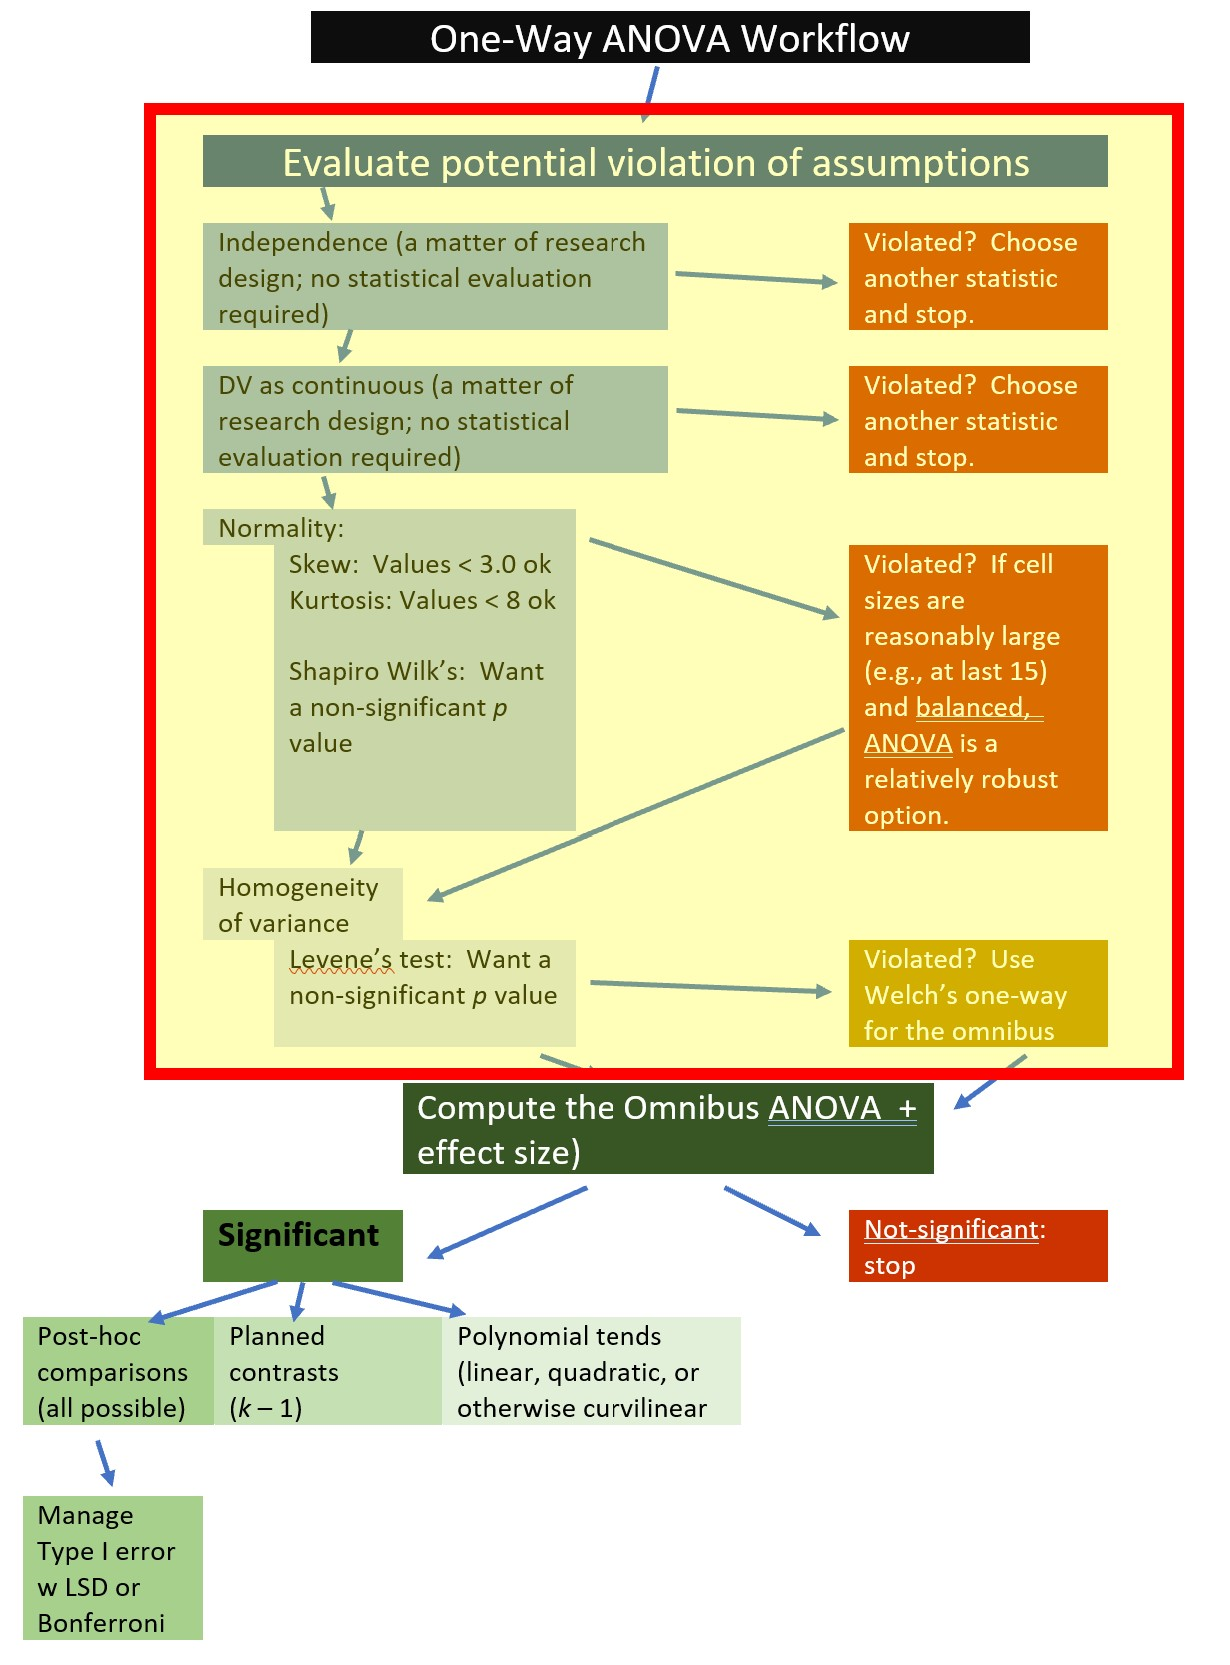
\includegraphics{images/oneway/OnewayWrkFlw_Asmptns.jpg}
\caption{An image of the workflow for one-way ANOVA, showing that we are at the beginning: evaluating the potential violation of the assumptions.}
\end{figure}

\hypertarget{evaluating-the-statistical-assumptions-3}{%
\subsection{Evaluating the Statistical Assumptions}\label{evaluating-the-statistical-assumptions-3}}

All statistical tests have some assumptions about the data. The one-way ANOVA has four assumptions:

\begin{itemize}
\tightlist
\item
  The dependent variable is normally distributed for each of the populations as defined by the different levels of the factor. We will examine this by

  \begin{itemize}
  \tightlist
  \item
    evaluating skew and kurtosis
  \item
    visually inspecting the distribution
  \item
    conducting Shapiro-Wilk tests of normality
  \item
    examing a QQ plot
  \end{itemize}
\item
  The variances of the dependent variable are the same for all populations. This is often termed the \emph{homogeneity of variance} assumption. We will examine this with

  \begin{itemize}
  \tightlist
  \item
    Levene's Test
  \end{itemize}
\item
  The cases represent \emph{random} samples from the populations and scores on the test variable are \emph{independent} of each other. That is, comparing related cases (e.g., parent/child, manager/employee, time1/time2) violates this assumption and this question would need to be evaluated by a different statistic such as \protect\hyperlink{Repeated}{repeated measures ANOVA} or dyadic data analysis.

  \begin{itemize}
  \tightlist
  \item
    \emph{Independence} in observations is a research design issue. ANOVA is not robust to violating this assumption. When observations are correlated/dependent there is a dramatic increase in Type I error.
  \end{itemize}
\item
  The dependent variable is measured on an interval scale.

  \begin{itemize}
  \tightlist
  \item
    If the dependent variable is categorical, another statistic (such as logistic regression) should be chosen.
  \end{itemize}
\end{itemize}

\hypertarget{is-the-dependent-variable-normally-distributed-across-levels-of-the-factor}{%
\subsubsection{Is the dependent variable normally distributed across levels of the factor?}\label{is-the-dependent-variable-normally-distributed-across-levels-of-the-factor}}

From the \emph{psych} package, the \emph{describe()} function can be used to provide descriptive statistics (or, ``descriptives'') of continuously scaled variables (i.e., variables measured on the interval or ratio scale). In this simple example, we can specify the specific continuous, DV.

\begin{Shaded}
\begin{Highlighting}[]
\CommentTok{\# we name the function in parentheses we list data source}
\NormalTok{psych}\SpecialCharTok{::}\FunctionTok{describe}\NormalTok{(accSIM30}\SpecialCharTok{$}\NormalTok{Accurate, }\AttributeTok{type =} \DecValTok{1}\NormalTok{)  }\CommentTok{\#the type=1 argument provides the specific skew and kurtosis values for which Kline\textquotesingle{}s recommendations are intended}
\end{Highlighting}
\end{Shaded}

\begin{verbatim}
   vars  n mean   sd median trimmed  mad min max range  skew kurtosis   se
X1    1 90  1.6 0.67   1.73    1.62 0.68   0   3     3 -0.29    -0.43 0.07
\end{verbatim}

If we want descriptives for each level of the grouping variable (factor), we can use the \emph{describeBy()} function of the \emph{psych} package. The order of entry within the script is the DV followed by the grouping variable (IV). In our research vignette below, I mentally interpret the \emph{Accurate \textasciitilde{} COND} formula as, ``Accurate by condition.''

\begin{Shaded}
\begin{Highlighting}[]
\CommentTok{\# It is unnecessary to create an object, but an object allows you to}
\CommentTok{\# do cool stuff, like write it to a .csv file and use that as a basis}
\CommentTok{\# for APA style tables In this script we can think \textquotesingle{}Accurate by COND\textquotesingle{}}
\CommentTok{\# meaning that the descriptives for accuracy will be grouped by COND}
\CommentTok{\# which is a categorical variable mat = TRUE presents the output in}
\CommentTok{\# matrix (table) form digits = 3 rounds the output to 3 decimal}
\CommentTok{\# places data = accSIM30 is a different (I think easier) way to}
\CommentTok{\# identify the object that holds the dataframe}
\NormalTok{des.mat }\OtherTok{\textless{}{-}}\NormalTok{ psych}\SpecialCharTok{::}\FunctionTok{describeBy}\NormalTok{(Accurate }\SpecialCharTok{\textasciitilde{}}\NormalTok{ COND, }\AttributeTok{mat =} \ConstantTok{TRUE}\NormalTok{, }\AttributeTok{digits =} \DecValTok{3}\NormalTok{, }\AttributeTok{data =}\NormalTok{ accSIM30,}
    \AttributeTok{type =} \DecValTok{1}\NormalTok{)}
\CommentTok{\# Note. Recently my students and I have been having intermittent}
\CommentTok{\# struggles with the describeBy function in the psych package. We}
\CommentTok{\# have noticed that it is problematic when using .rds files and when}
\CommentTok{\# using data directly imported from Qualtrics. If you are having}
\CommentTok{\# similar difficulties, try uploading the .csv file and making the}
\CommentTok{\# appropriate formatting changes. displays the matrix object that we}
\CommentTok{\# just created}
\NormalTok{des.mat}
\end{Highlighting}
\end{Shaded}

\begin{verbatim}
          item  group1 vars  n  mean    sd median trimmed   mad   min   max
Accurate1    1 Control    1 30 1.756 0.460  1.893   1.767 0.392 0.781 2.745
Accurate2    2     Low    1 30 1.900 0.630  2.007   1.918 0.458 0.655 3.000
Accurate3    3    High    1 30 1.153 0.659  1.131   1.128 0.743 0.000 2.669
          range   skew kurtosis    se
Accurate1 1.964 -0.289   -0.364 0.084
Accurate2 2.345 -0.398   -0.288 0.115
Accurate3 2.669  0.218   -0.528 0.120
\end{verbatim}

\begin{Shaded}
\begin{Highlighting}[]
\CommentTok{\# optional to write it to a .csv file for further manipulation and}
\CommentTok{\# formatting for a paper or presentation}
\FunctionTok{write.csv}\NormalTok{(des.mat, }\AttributeTok{file =} \StringTok{"Table1.csv"}\NormalTok{)}
\end{Highlighting}
\end{Shaded}

Skew and kurtosis are one way to evaluate whether or not data are normally distributed. When we use the ``type=1'' argument, the skew and kurtosis indices in the \emph{psych} package can be interpreted according to Kline's \citeyearpar{kline_data_2016} guidelines. Regarding skew, values greater than the absolute value of 3.0 are generally considered ``severely skewed.'' Regarding kurtosis, ``severely kurtotic'' is argued to be anywhere greater 8 to 20. Kline recommended using a conservative threshold of the absolute value of 10.

The \emph{Shapiro-Wilk} test evaluates the hypothesis that the distribution of the data deviates from a comparable normal distribution. If the test is non-significant (\emph{p} \textgreater.05) the distribution of the sample is not significantly different from a normal distribution. If, however, the test is significant (\emph{p} \textless{} .05), then the sample distribution is significantly different from a normal distribution. The \emph{rstatix} package can conduct this test for us.

\begin{Shaded}
\begin{Highlighting}[]
\FunctionTok{library}\NormalTok{(tidyverse)}
\NormalTok{shapiro }\OtherTok{\textless{}{-}}\NormalTok{ accSIM30 }\SpecialCharTok{\%\textgreater{}\%}
    \FunctionTok{group\_by}\NormalTok{(COND) }\SpecialCharTok{\%\textgreater{}\%}
\NormalTok{    rstatix}\SpecialCharTok{::}\FunctionTok{shapiro\_test}\NormalTok{(Accurate)}
\NormalTok{shapiro}
\end{Highlighting}
\end{Shaded}

\begin{verbatim}
# A tibble: 3 x 4
  COND    variable statistic     p
  <fct>   <chr>        <dbl> <dbl>
1 Control Accurate     0.954 0.215
2 Low     Accurate     0.944 0.115
3 High    Accurate     0.980 0.831
\end{verbatim}

The \(p\) values for the distributions of the dependent variable (accurate) in each of the three conditions are all well above .05. This tells us that the Accurate variable does not deviate from a statistically significant distribution at any level (Control, \emph{W} = 0.954, \emph{p} = 0.215; Low, \emph{W} = 0.944, \emph{p} = 0.115`; High, \emph{W} = 0.980, \emph{p} = 0.831).

Especially in the more simple ``ANOVA's'' I like this form of the Shapiro-Wilk test because it makes it clear that we expect normality within each of the grouping levels. This approach, however, is only appropriate when there are a low number of levels/groupings and there are many data points per group. As models become more complex, researchers should use the model-based option for assessing normality. To do this, we first create an object that tests our research model.

Although that model (a regression model) has information about our primary statistic, we are using it to carefully investigate the assumption of normality. One product of the analysis is \emph{residuals}. Residuals are the unexplained variance in the outcome (or dependent) variable after accounting for the predictor (or independent) variable. When we plot these ``leftovers'' against the values of x, we can visualize the fit of the model in a QQ plot. The dots represent the residuals. When they are relatively close to the line they not only suggest good fit of the model, but we know they are small and evenly distributed around zero (i.e., normally distributed).

\begin{Shaded}
\begin{Highlighting}[]
\NormalTok{res\_model }\OtherTok{\textless{}{-}} \FunctionTok{lm}\NormalTok{(Accurate }\SpecialCharTok{\textasciitilde{}}\NormalTok{ COND, }\AttributeTok{data =}\NormalTok{ accSIM30)}
\NormalTok{ggpubr}\SpecialCharTok{::}\FunctionTok{ggqqplot}\NormalTok{(}\FunctionTok{residuals}\NormalTok{(res\_model))}
\end{Highlighting}
\end{Shaded}

\includegraphics{07-OnewayANOVA_files/figure-latex/unnamed-chunk-45-1.pdf} We can also use the model in a Shapiro-Wilk test. As before, we want a non-significant result.

\begin{Shaded}
\begin{Highlighting}[]
\NormalTok{rstatix}\SpecialCharTok{::}\FunctionTok{shapiro\_test}\NormalTok{(}\FunctionTok{residuals}\NormalTok{(res\_model))}
\end{Highlighting}
\end{Shaded}

\begin{verbatim}
# A tibble: 1 x 3
  variable             statistic p.value
  <chr>                    <dbl>   <dbl>
1 residuals(res_model)     0.979   0.150
\end{verbatim}

These results parallel what we have already learned. That is, the non-significant \emph{p} value associated with the model-based Shapiro-Wilk test of normality indicates that our distribution of residuals does not differ from a normal distribution (\(W = 0.979, p = 0.15\)). Given the space restrictions in journal articles and the greater interest in results of the primary analyses, I am more likely to report model-level results than the results from the cell-based Shapiro-Wilk tests.

There are limitations to the Shapiro-Wilk test. As the dataset being evaluated gets larger, the Shapiro-Wilk test becomes more sensitive to small deviations; this leads to a greater probability of rejecting the null hypothesis (null hypothesis being the values come from a normal distribution). Green and Salkind \citeyearpar{green_using_2017} advised that ANOVA is relatively robust to violations of normality if there are at least 15 cases per cell and the design is reasonably balanced (i.e., equal cell sizes).

\hypertarget{should-we-consider-removing-outliers}{%
\subsubsection{Should we consider removing outliers?}\label{should-we-consider-removing-outliers}}

If our data pointed to significant violations of normality, we could consider identifying and removing outliers. Removing data is a serious consideration that should not be made lightly. If needed, though, here is a tool to inspect the data and then, if necessary, remove it.

We can think of outlier identification in a couple of ways. First, we might look at dependent variable across the entire dataset. That is, without regard to the levels of the grouping variable. We can point \emph{rstatix::identify\_outliers()} to the data.

\begin{Shaded}
\begin{Highlighting}[]
\NormalTok{accSIM30 }\SpecialCharTok{\%\textgreater{}\%}
\NormalTok{    rstatix}\SpecialCharTok{::}\FunctionTok{identify\_outliers}\NormalTok{(Accurate)}
\end{Highlighting}
\end{Shaded}

\begin{verbatim}
[1] ID         COND       Accurate   moreTalk   m_dev      m_devSQ    is.outlier
[8] is.extreme
<0 rows> (or 0-length row.names)
\end{verbatim}

The output ``0 rows'' is not an error. It means if we consider the distribution of the Accurate variable as a whole, there are no outliers. Let's re-run the code, this time requiring it to look within each of the grouping levels of the condition variable.

\begin{Shaded}
\begin{Highlighting}[]
\NormalTok{accSIM30 }\SpecialCharTok{\%\textgreater{}\%}
    \FunctionTok{group\_by}\NormalTok{(COND) }\SpecialCharTok{\%\textgreater{}\%}
\NormalTok{    rstatix}\SpecialCharTok{::}\FunctionTok{identify\_outliers}\NormalTok{(Accurate)}
\end{Highlighting}
\end{Shaded}

\begin{verbatim}
# A tibble: 2 x 8
  COND  ID    Accurate moreTalk  m_dev m_devSQ is.outlier is.extreme
  <fct> <fct>    <dbl>    <dbl>  <dbl>   <dbl> <lgl>      <lgl>     
1 Low   31       0.663   -1.10  -0.940   0.884 TRUE       FALSE     
2 Low   39       0.655   -0.201 -0.948   0.899 TRUE       FALSE     
\end{verbatim}

This output tells us that in the low-racial loading condition there are two cases that are identified as outliers (denoted as TRUE) but not as extreme outliers (denoted as FALSE). Handily, the function returns information (i.e., the values of the Accurate and moreTalk variables, the ID number) that would help us delete it.

Let's say that, after very careful consideration, we decided to remove the case with ID = 31. We could use \emph{dplyr::filter()} to do so. In this code, the \emph{filter()} function locates all the cases where ID = 31. The exclamation point that precedes the equal sign indicates that the purpose is to remove the case.

\begin{Shaded}
\begin{Highlighting}[]
\CommentTok{\# accSIM30 \textless{}{-} dplyr::filter (accSIM30, ID != \textquotesingle{}31\textquotesingle{})}
\end{Highlighting}
\end{Shaded}

Once executed, we can see that this case is no longer in the dataframe. Although I demonstrated this in the accompanying lecture, I have hashtagged out the command because I would not delete the case. If you already deleted the case, you can return the hashtag and re-run all the code up to this point.

\hypertarget{are-the-variances-of-the-dependent-variable-similar-across-the-levels-of-the-grouping-factor-1}{%
\subsubsection{Are the variances of the dependent variable similar across the levels of the grouping factor?}\label{are-the-variances-of-the-dependent-variable-similar-across-the-levels-of-the-grouping-factor-1}}

The Levene's test evaluates the ANOVA assumption that variances of the dependent variable for each level of the independent variable are similarly distributed. We want this to be non-significant (\(p\) \textgreater{} .05). If violated, we need to use an ANOVA test that is ``robust to the violation of the homogeneity of variance'' (e.g., Welch's oneway).

\begin{Shaded}
\begin{Highlighting}[]
\NormalTok{rstatix}\SpecialCharTok{::}\FunctionTok{levene\_test}\NormalTok{(accSIM30, Accurate }\SpecialCharTok{\textasciitilde{}}\NormalTok{ COND)}
\end{Highlighting}
\end{Shaded}

\begin{verbatim}
# A tibble: 1 x 4
    df1   df2 statistic     p
  <int> <int>     <dbl> <dbl>
1     2    87      1.70 0.190
\end{verbatim}

We write the result of the Levene's as \(F(2, 87) = 1.695, p = 0.190\). Because \(p\) \textgreater{} .05, we know that the result is nonsignficant -- that the variances of the three groups are not statistically significantly different from each other. If the results had been statistically significantly different, we would have needed to use a Welch's \(F\) or robust version of ANOVA.

\hypertarget{summarizing-results-from-the-analysis-of-assumptions}{%
\subsubsection{Summarizing results from the analysis of assumptions}\label{summarizing-results-from-the-analysis-of-assumptions}}

It is common for an APA style results section to begin with a review of the evaluation of the statistical assumptions. As we have just finished these analyses, I will document what we have learned so far:

\begin{quote}
Regarding the assumption of normality, skew and kurtosis values at each of the levels of the condition value fell well below the thresholds that Kline \citeyearpar{kline_data_2016} identified as concerning (i.e., below \textbar3\textbar{} for skew and \textbar10\textbar{} for kurtosis). Similarly, no extreme outliers were identified and results of a model-based Shapiro-Wilk test of normality, indicated that the model residuals did not did differ from a normal distribution \((W = 0.979, p = 0.15)\). Finally, Levene's homogeneity of variance test indicated no violation of the homogeneity of variance assumption (\(F[2, 87] = 1.695, p = 0.190\)).
\end{quote}

\hypertarget{computing-the-omnibus-anova}{%
\subsection{Computing the Omnibus ANOVA}\label{computing-the-omnibus-anova}}

Having met all the assumptions, we are now ready to calculate the omnibus \(F\) test. \emph{Omnibus} is the term applied to the first \emph{F} test that evaluates if all groups have the same mean \citep{chen_relationship_2018}. If this test is not significant there is no evidence in the data to reject the null; that is, there is no evidence to suggest that group means are different. If it is significant -- and there are three or more groups -- follow-up testing will be needed to determine where the differences lie.

\begin{figure}
\centering
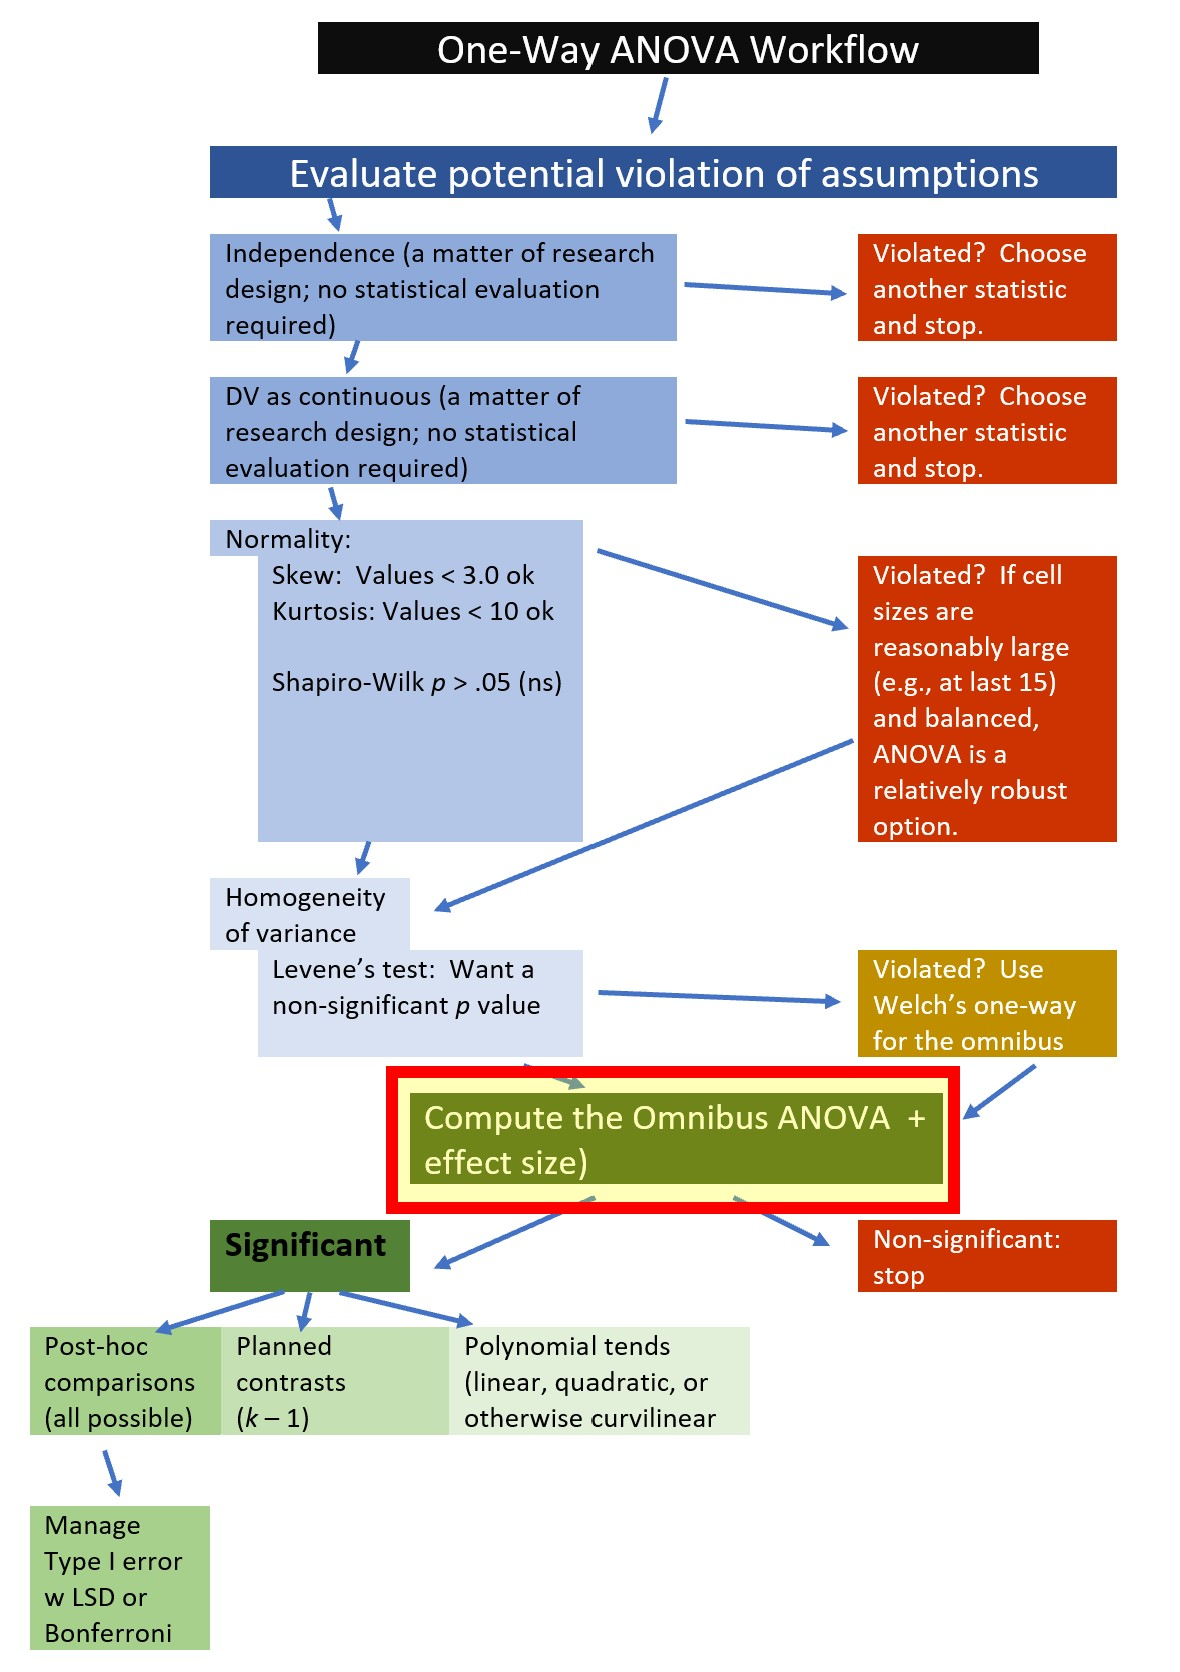
\includegraphics{images/oneway/OnewayWrkFlw_omnibus.jpg}
\caption{An image of the workflow for one-way ANOVA, showing that we are at the stage of computing the omnibus ANOVA.}
\end{figure}

We will use \emph{rstatix::anova\_test} to calculate the omnibus. In script we must point to the data and provide the formula (Accurate \textasciitilde{} COND). By specifying ``detailed=TRUE'' we get can view our sums of squares values. When we run this test, we will save all of the results in an object. We can name this object anything -- I will call it \emph{omnibus1w}. When we create objects, we have to re-type the name of the object below our formula in order for the results to display. Objects are incredibly useful because we can later use them in follow-up tests, in creating figures, and in exporting results that we can use outside of R (e.g., to create tables for papers or presentations).

\begin{Shaded}
\begin{Highlighting}[]
\NormalTok{omnibus1w }\OtherTok{\textless{}{-}}\NormalTok{ rstatix}\SpecialCharTok{::}\FunctionTok{anova\_test}\NormalTok{(accSIM30, Accurate }\SpecialCharTok{\textasciitilde{}}\NormalTok{ COND, }\AttributeTok{detailed =} \ConstantTok{FALSE}\NormalTok{)}
\NormalTok{omnibus1w}
\end{Highlighting}
\end{Shaded}

\begin{verbatim}
ANOVA Table (type II tests)

  Effect DFn DFd      F          p p<.05   ges
1   COND   2  87 13.566 0.00000745     * 0.238
\end{verbatim}

The values we see map onto those we calculated by hand. Our \(SS_M\) (9.432) plus \(SS_R\) (30.246) sum to equal the \(SS_T\) (39.678). Dividing the two sums of squares by their respective degrees of freedom produces the means squared. Then, dividing the \(MS_M\) (COND) by \(MS_R\) (4.716/0.348) provides the \emph{F} ratio. By using a table of \emph{F} critical values, we already knew that our \emph{F} value exceeded the value in the table of critical values. Here we see that \emph{p} \textless{} .001.

The ``\emph{F} string'' for an APA style results section should be written like this: \(F(2,87) = 13.566, p < .001\).

\hypertarget{effect-size-for-the-one-way-anova}{%
\subsubsection{Effect size for the one-way ANOVA}\label{effect-size-for-the-one-way-anova}}

\textbf{Eta squared} is one of the most commonly used measures of effect. It refers to the proportion of variability in the dependent variable/outcome that can be explained in terms of the independent variable/predictor. Conventionally, values of .01, .06, and .14 are considered to be small, medium, and large effect sizes, respectively.

You may see different values (.02, .13, .26) suggested as small, medium, and large effects -- these values are used when multiple regression is used. A useful summary of effect sizes, guide to interpreting their magnitudes, and common usage can be found \href{https://imaging.mrc-cbu.cam.ac.uk/statswiki/FAQ/effectSize}{here} \citep{watson_rules_2020}.

The formula for \(\eta^2\) is straightforward. If we think back to our hand-calculations of all the sums of squares, we can see that this is the proportion of variance that is accounted for by the model.

\[\eta ^{2}=\frac{SS_{M}}{SS_{T}}\] Hand calculation, then, is straightforward.:

\begin{Shaded}
\begin{Highlighting}[]
\FloatTok{9.432}\SpecialCharTok{/}\NormalTok{(}\FloatTok{9.432} \SpecialCharTok{+} \FloatTok{30.246}\NormalTok{)}
\end{Highlighting}
\end{Shaded}

\begin{verbatim}
[1] 0.2377136
\end{verbatim}

Luckily, \emph{rstatix::anova\_test()} has provided the \(\eta ^{2}\) for us; it is found in the column, \emph{ges}. Using the interpretive criteria suggests that our effect is rather large. We can update our \emph{F} string this way: \(F(2,87) = 13.566, p < .001, \eta ^{2} = 0.238\). An APA style write-up of the omnibus might read like this:

\begin{quote}
Results of the omnibus ANOVA indicated a significant effect of COND on accuracy perception \((F[2,87] = 13.566, p < .001, \eta ^{2} = 0.238)\).
\end{quote}

\hypertarget{follow-up-to-the-omnibus-f}{%
\subsection{\texorpdfstring{Follow-up to the Omnibus \emph{F}}{Follow-up to the Omnibus F}}\label{follow-up-to-the-omnibus-f}}

The \emph{F}-test associated with the one-way ANOVA is the \emph{omnibus} -- giving the result for the overall test. Looking at the workflow for the one-way ANOVA we see that if we had had we had a non-significant \(F\), we would have stopped our analysis.

However, if the omnibus \(F\) is significant, we know that there is at least one pair of cells where there is a statistically significant difference. We have several ways (each with its own strengths/limitations) to figure out where these differences lie.

\hypertarget{planning-for-the-management-of-type-i-error}{%
\subsubsection{Planning for the management of Type I Error}\label{planning-for-the-management-of-type-i-error}}

\emph{Type I error} is the concern about false positives -- that we would incorrectly reject a true null hypothesis (i.e., claiming a statistically significant difference when there is not one). In ANOVA, we become increasingly concerned about Type I error as the number of pairwise or post hoc comparison increases. In ANOVA, we generally begin controlling for Type I error when follow-up to a significant omnibus test.

The \emph{traditional Bonferroni} is, perhaps, the most well-known approach to managing Type I error. Although the lessons in this OER will frequently suggest alternative approaches to managing Type I error, I will quickly review it now because it is relatively straightforward and intuitive. We start by establishing the \(\alpha_{family}\); this is traditionally \(p = .05\).

Next, we determine how many pairwise comparisons that we are going to conduct. If we want to conduct all possible comparisons, we could use this formula to determing the number: \(N_{pc}=\frac{N_{g}(N_{g}-1)}{2}\), where

\begin{itemize}
\tightlist
\item
  \(N_{pc}\) is the number of pairwise comparisons, and
\item
  \(N_{g}\) is the number of groups.
\end{itemize}

In the current research vignette, the COND factor had three levels: control, low, high. Thus, if we wanted to conduct all possible comparisons we would determine \(N_{pc}\) this way:

\begin{Shaded}
\begin{Highlighting}[]
\DecValTok{3}\SpecialCharTok{*}\NormalTok{(}\DecValTok{3{-}1}\NormalTok{)}\SpecialCharTok{/}\DecValTok{2}
\end{Highlighting}
\end{Shaded}

\begin{verbatim}
[1] 3
\end{verbatim}

Subsequently, we would compute a new alpha that would be used for each comparison with this formula: \(\alpha_{pc}=\frac{\alpha_{family}}{N_{pc}}\).

In the current research vignette we would calculate it this way:

\begin{Shaded}
\begin{Highlighting}[]
\NormalTok{.}\DecValTok{05}\SpecialCharTok{/}\DecValTok{3}
\end{Highlighting}
\end{Shaded}

\begin{verbatim}
[1] 0.01666667
\end{verbatim}

If we were to use the traditional Bonferroni to manage Type I error, the resultant \(p\) value would need to be \textless{} .017 in order for statistical significance to be claimed.

Luckily, the traditional Bonferroni (and other approaches to managing Type I error) has been reverse-engineered so that we do not have to determine the more conservative alpha levels. Rather, when we specify these options in the R script, the \emph{p} value is adjusted and we can continue to use the customary criteria of \(p < .05, p < .01\), and \(p < .001\). In the case of the traditional Bonferonni, the \emph{p} value has been adjusted upward by multiplying it (i.e., the raw \emph{p} values) by the number of comparisons being completed. This holds the \emph{total} Type I error rate across these tests to be \(\alpha = 0.05\).

Although the traditional Bonferroni is easy-to-understand and compute, it has been criticized as being too restrictive. That is, it increases the risk of making a Type II error (i.e., failing to reject the null hypothesis when it is false). Therefore, as we work through each option for follow-up testing for the ANOVA models, I will introduce one or more methods for managing Type I error that are commonly used with that follow-up. Descriptions of all the methods for managing Type I error that are used in this OER are described in an \protect\hyperlink{type1}{appendix}

\hypertarget{option-1-post-hoc-pairwise-comparisons}{%
\subsubsection{OPTION \#1: Post hoc, pairwise, comparisons}\label{option-1-post-hoc-pairwise-comparisons}}

A very common follow-up to the omnibus test from a one-way ANOVA is to conduct post hoc, pairwise comparisons, of all possible combinations of pairs.

\begin{figure}
\centering
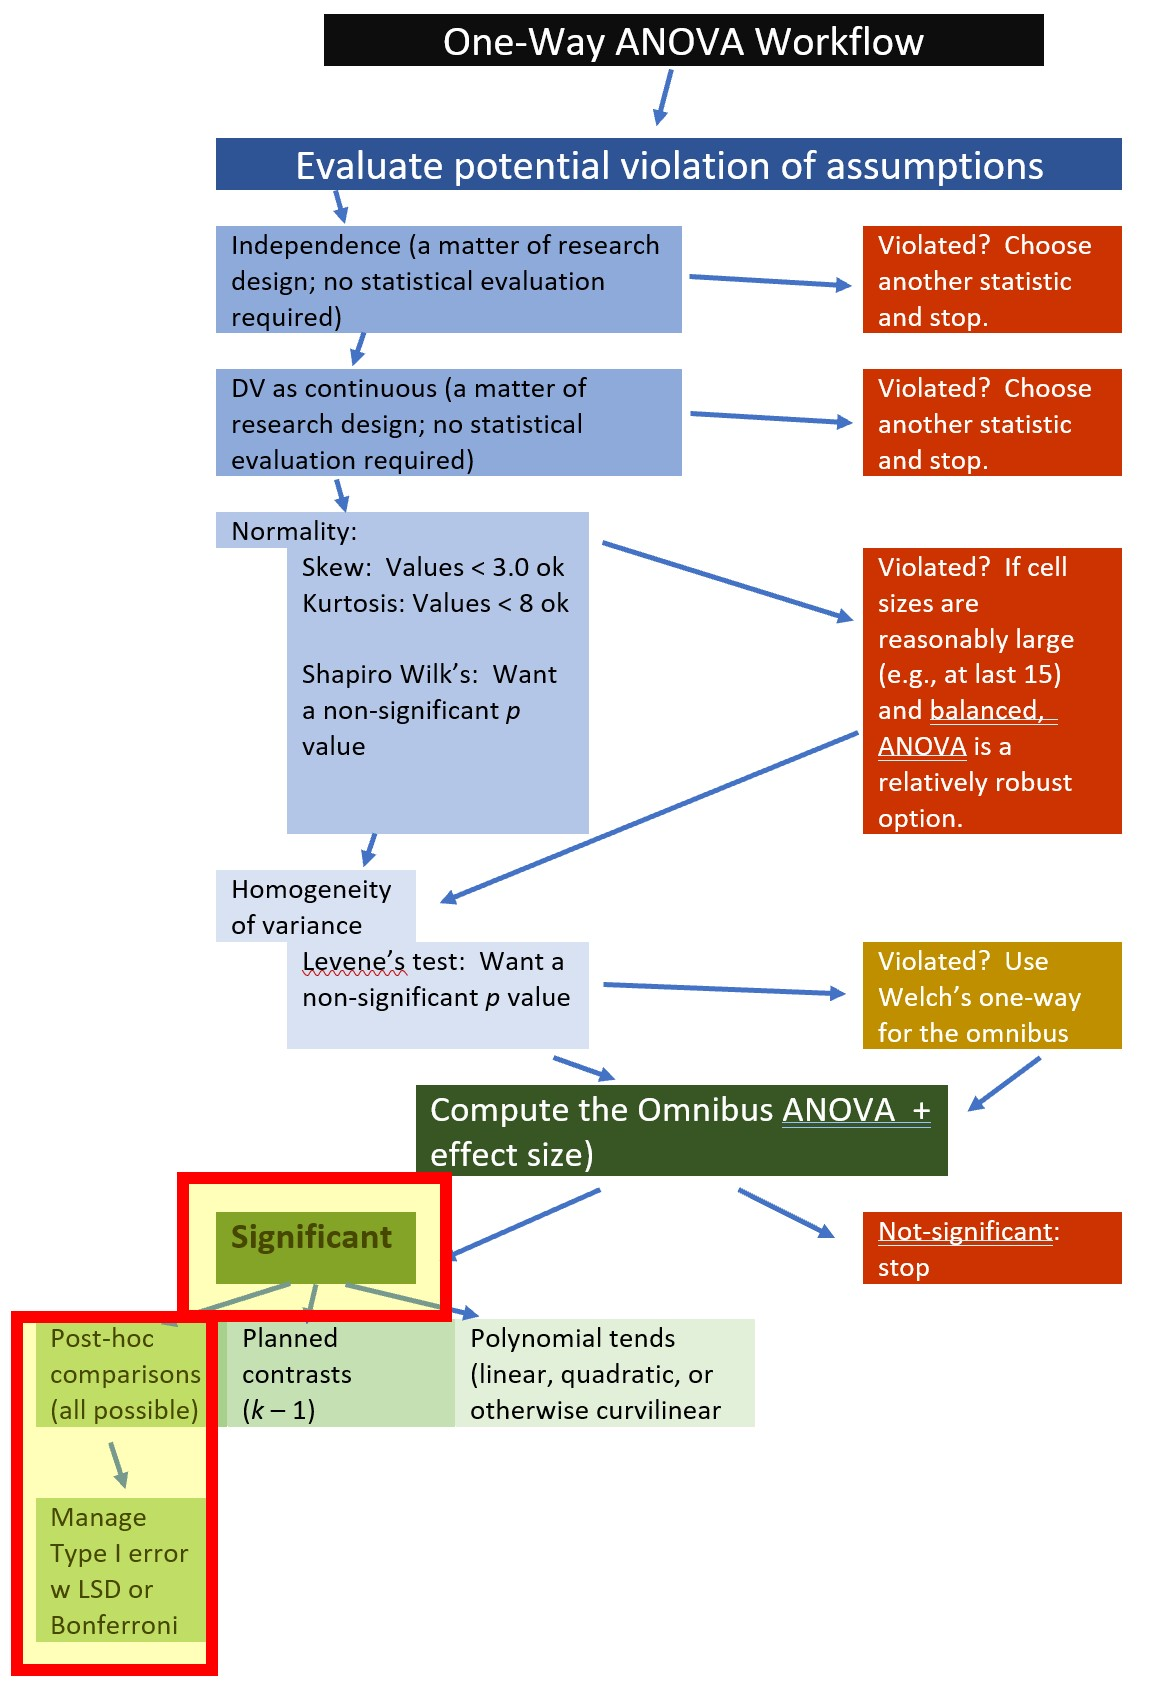
\includegraphics{images/oneway/OnewayWrkFlw_phoc.jpg}
\caption{An image of the workflow for one-way ANOVA, showing that we are at the stage of following a statistically significant omnibus F test and are now conducting post hoc comparisons.}
\end{figure}

Post hoc, pairwise comparisons are:

\begin{itemize}
\tightlist
\item
  used for exploratory work when no firm hypotheses were articulated a priori,
\item
  used to compare the means of all combinations of pairs of an experimental condition,
\item
  less powerful than planned comparisons because more strict criterion for significance should be used.
\end{itemize}

By specifying the \emph{formula} of the ANOVA, the \emph{rstatix::t\_test()} function will provide comparisons of all possible combinations. The arguments in the code mirror those we used for the omnibus. Note that I am saving the results as an object. We will use this object (``ttest'') later when we create an accompanying figure.

We will request the traditional Bonferroni using the \emph{p.adjust.method}. The \emph{rstatix::t\_test()} offers multiple options for adjusting the \emph{p} values.

\begin{Shaded}
\begin{Highlighting}[]
\NormalTok{ttest }\OtherTok{\textless{}{-}}\NormalTok{ rstatix}\SpecialCharTok{::}\FunctionTok{t\_test}\NormalTok{(accSIM30, Accurate }\SpecialCharTok{\textasciitilde{}}\NormalTok{ COND, }\AttributeTok{p.adjust.method =} \StringTok{"bonferroni"}\NormalTok{,}
    \AttributeTok{detailed =} \ConstantTok{TRUE}\NormalTok{)}
\NormalTok{ttest}
\end{Highlighting}
\end{Shaded}

\begin{verbatim}
# A tibble: 3 x 17
  estimate estimate1 estimate2 .y.   group1 group2    n1    n2 statistic       p
*    <dbl>     <dbl>     <dbl> <chr> <chr>  <chr>  <int> <int>     <dbl>   <dbl>
1   -0.144      1.76      1.90 Accu~ Contr~ Low       30    30     -1.01 3.17e-1
2    0.603      1.76      1.15 Accu~ Contr~ High      30    30      4.11 1.4 e-4
3    0.747      1.90      1.15 Accu~ Low    High      30    30      4.49 3.45e-5
# i 7 more variables: df <dbl>, conf.low <dbl>, conf.high <dbl>, method <chr>,
#   alternative <chr>, p.adj <dbl>, p.adj.signif <chr>
\end{verbatim}

The \emph{estimate} column provide the mean difference between the two levels of the independent different. The \emph{estimate1/group1} and \emph{estimate2/group2} columns provide those means and identify the group levels. The \emph{statistic} column provides the value of the \emph{t}-test.

The \emph{p} value is the unadjusted \emph{p}-value, it will usually be ``more significant'' (i.e., a lower value) than the \emph{p.adj} value that we specified in our code. The column \emph{p.adj.signif} provides symbolic notation associated with the ``p.adj'' value. In this specific case we specified the traditional Bonferroni as the adjusted \emph{p} value.

An APA style results section of this follow-up might read like this:

\begin{quote}
We followed up the significant omnibus with a series of post hoc, pairwise comparisons. We controlled for Type I error with the traditional Bonferroni adjustment. Results suggested that there were statistically significant differences between the control and high (\(M_{diff} = 0.601, p < .001\)) and low and high (\(M_{diff} = 0.75, p < 0.001\)) conditions, but not control and low conditions (\(M_{diff} = -.14, p = 0.951\)). Consequently, it appeared that only the highest degree of racial loading (e.g., ``You speak English well for an Asian'') resulted in the decreased perceptions of accuracy of impressions from the confederate. Means and standard deviations are presented in Table 1 and complete ANOVA results are presented in Table 2. Figure 1 provides an illustration of the results.
\end{quote}

Below is an augmentation of the figure that appeared at the beginning of the chapter. We can use the objects from the omnibus tests (named, ``omnibus1w'') and post hoc pairwise comparisons (``ttest'') to add the ANOVA string and significance bars to the figure. Although they may not be appropriate in every circumstance, such detail can assist the figure in conveying maximal amounts of information.

\begin{Shaded}
\begin{Highlighting}[]
\CommentTok{\# updates the ttest object so that it will auto{-}compute p{-}value}
\CommentTok{\# positions in the graph}
\NormalTok{ttest }\OtherTok{\textless{}{-}}\NormalTok{ ttest }\SpecialCharTok{\%\textgreater{}\%}
\NormalTok{    rstatix}\SpecialCharTok{::}\FunctionTok{add\_xy\_position}\NormalTok{(}\AttributeTok{x =} \StringTok{"COND"}\NormalTok{)}

\CommentTok{\# our original plot}
\NormalTok{Fig1 }\OtherTok{\textless{}{-}}\NormalTok{ ggpubr}\SpecialCharTok{::}\FunctionTok{ggboxplot}\NormalTok{(accSIM30, }\AttributeTok{x =} \StringTok{"COND"}\NormalTok{, }\AttributeTok{y =} \StringTok{"Accurate"}\NormalTok{, }\AttributeTok{add =} \StringTok{"jitter"}\NormalTok{,}
    \AttributeTok{color =} \StringTok{"COND"}\NormalTok{, }\AttributeTok{title =} \StringTok{"Figure 1. Accuracy Perception as a Function of Racial Loading Condition"}\NormalTok{) }\SpecialCharTok{+}
\NormalTok{    ggpubr}\SpecialCharTok{::}\FunctionTok{stat\_pvalue\_manual}\NormalTok{(ttest, }\AttributeTok{label =} \StringTok{"p.adj.signif"}\NormalTok{, }\AttributeTok{tip.length =} \FloatTok{0.02}\NormalTok{,}
        \AttributeTok{hide.ns =} \ConstantTok{TRUE}\NormalTok{, }\AttributeTok{y.position =} \FunctionTok{c}\NormalTok{(}\FloatTok{3.25}\NormalTok{, }\FloatTok{3.75}\NormalTok{))}
\CommentTok{\# tip.length instructs how long to make the dropped edges of the}
\CommentTok{\# significance bar; hide.ns will suppress or display non{-}significant}
\CommentTok{\# bars; step.increase will separate the bars from each other so that}
\CommentTok{\# they do not overlap}

\NormalTok{Fig1}
\end{Highlighting}
\end{Shaded}

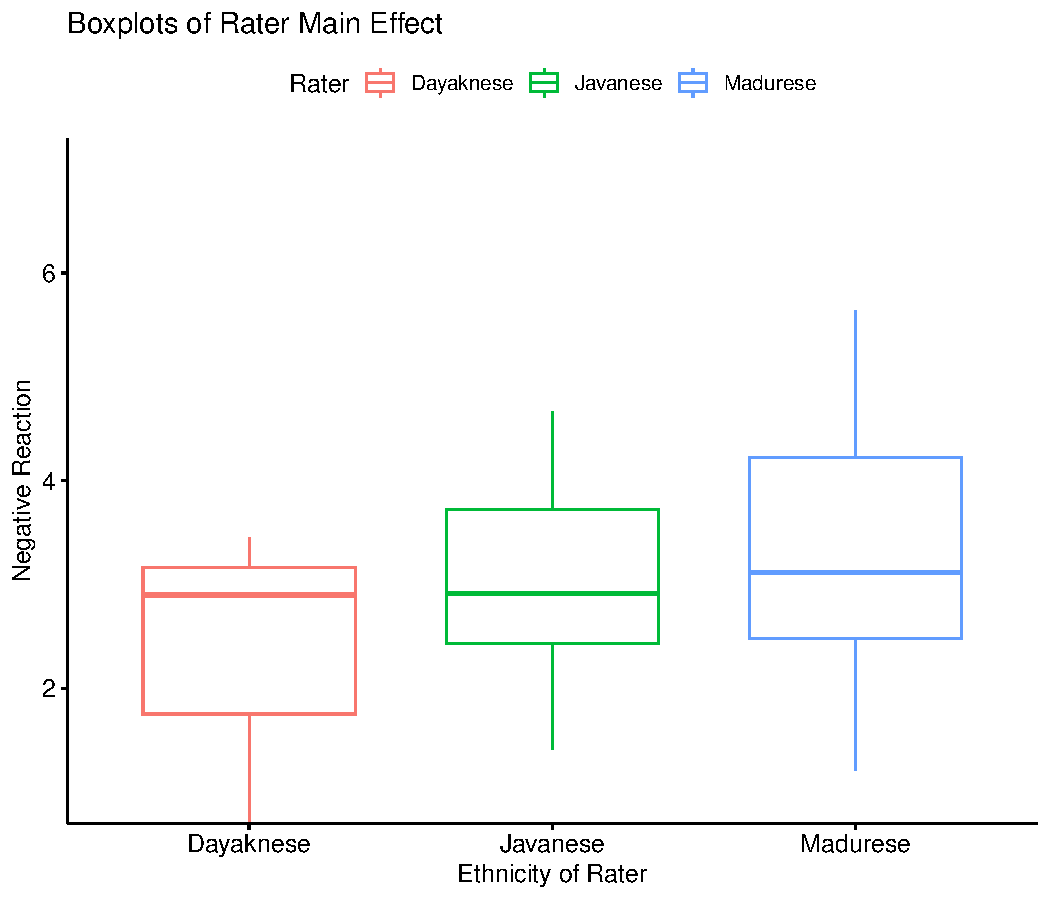
\includegraphics{07-OnewayANOVA_files/figure-latex/unnamed-chunk-56-1.pdf}

Although it would not make a difference in this research vignette, the LSD (least significant differences) method is commonly used for controlling Type I error in the follow-up to a one-way ANOVA. The LSD method is appropriate in the one-way ANOVA scenario when there are only three levels in the factor. In this case, Green and Salkind \citeyearpar{green_using_2017} have suggested that alpha could be retained at the alpha level for the ``family'' (\(\alpha_{family}\)), which is conventionally \(p = .05\) and used both to evaluate the omnibus and, so long as they don't exceed three in number, the planned or pairwise comparisons that follow.

\hypertarget{option-2-non-orthogonal-planned-contrast}{%
\subsubsection{OPTION \#2: Non-orthogonal planned contrast}\label{option-2-non-orthogonal-planned-contrast}}

Another option for follow-up to a significant omnibus test is to evaluate \emph{planned} comparisons. These can either be orthogonal (i.e., a complete partitioning of variance) or \emph{non-orthogonal} (i.e., allowing for overlapping variance). We will start with a non-orthogonal example.

\begin{figure}
\centering
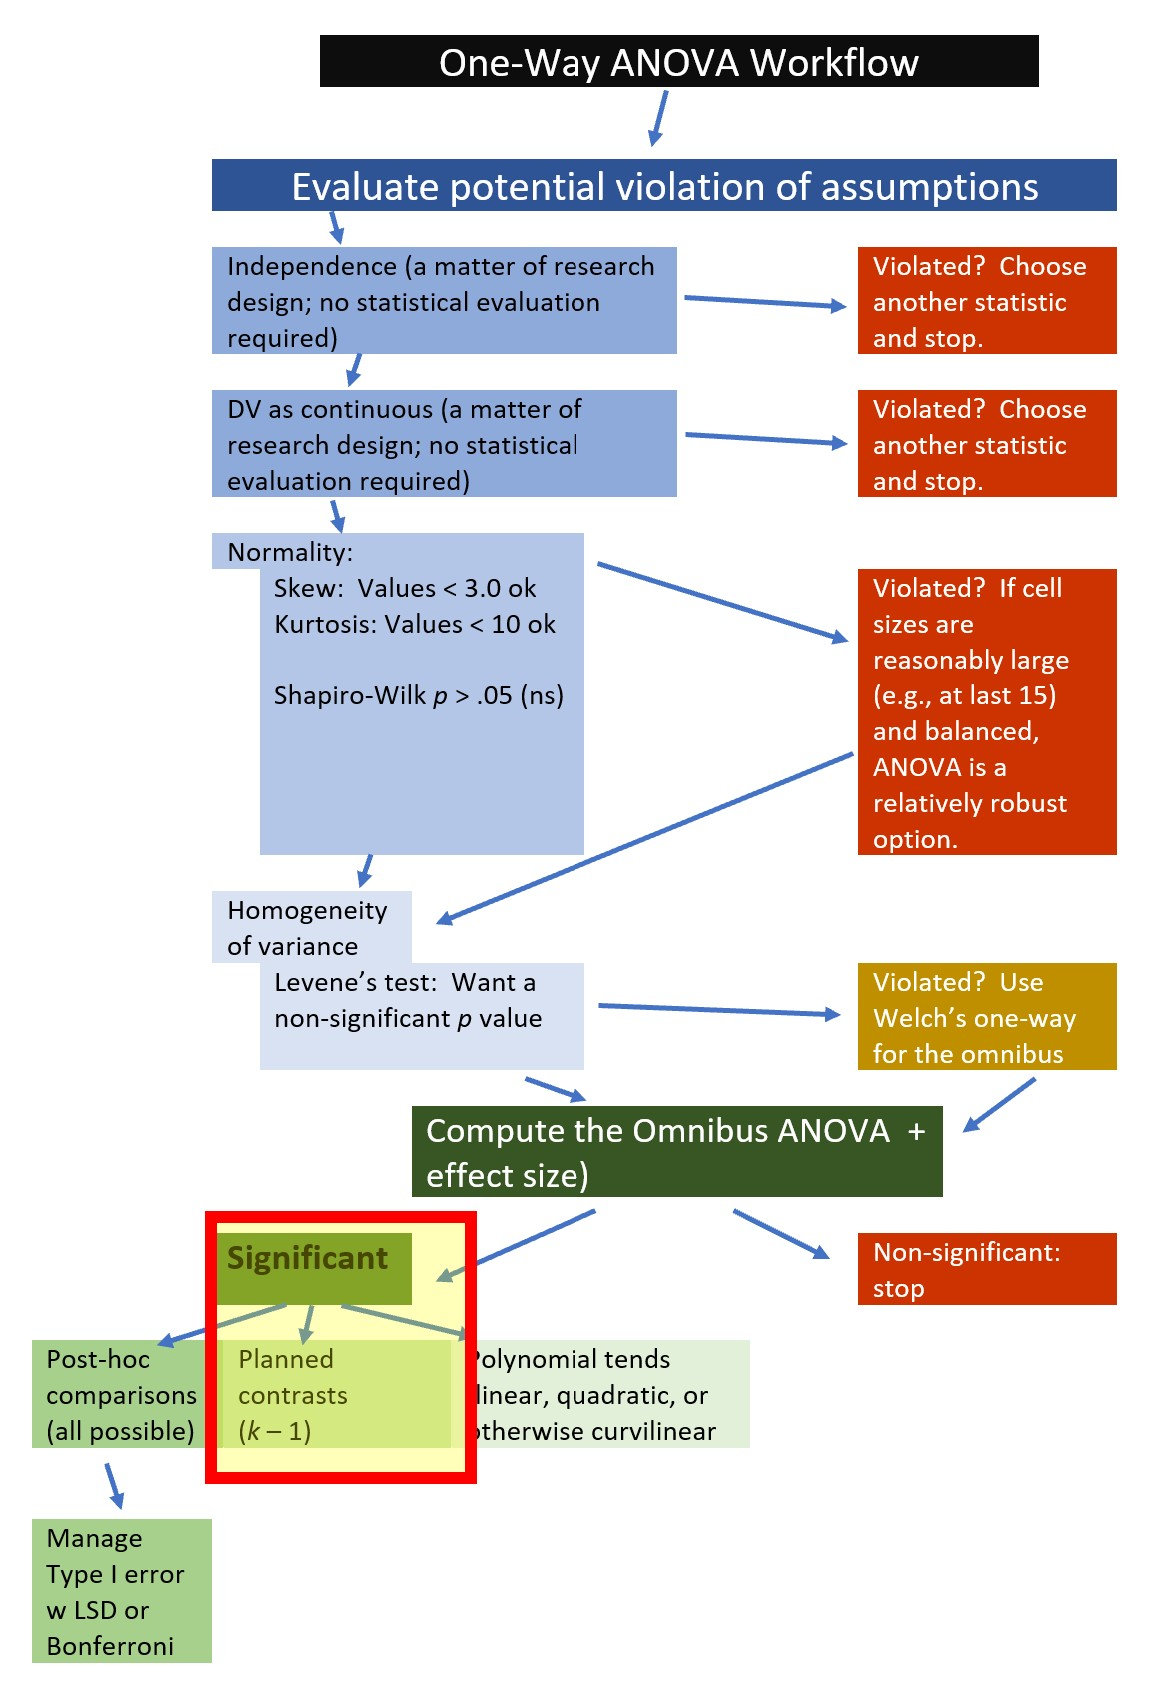
\includegraphics{images/oneway/OnewayWrkFlw_planned.jpg}
\caption{An image of the workflow for one-way ANOVA, showing that we are at the following up to a significant omnibus F by conducting planned comparisons}
\end{figure}

Planned comparisons are

\begin{itemize}
\tightlist
\item
  theory-driven comparisons constructed prior to data collection,
\item
  based on the idea of partitioning the variance created by the overall effect of group differences into gradually smaller portions of variance, and
\item
  more powerful than post hoc tests.
\end{itemize}

Planned contrasts involve further considerations regarding the \emph{partitioning of variance.}

\begin{itemize}
\tightlist
\item
  There will always be \(k-1\) contrasts; in our case this means we will have two contrasts
\item
  Each contrast must involve only two \emph{chunks} of variance.
\end{itemize}

If the researcher chooses this route, they must decide which two comparisons will best tell the story of the data as it relates to the hypotheses and a priori theory. I will compare differences between the no and low racial loading conditions, and then between low and high racial loading conditions. I have chosen to not adjust the \emph{p} values. In the results write-up, I will reference the LSD method as my rationale for this approach.

\begin{Shaded}
\begin{Highlighting}[]
\NormalTok{contr2 }\OtherTok{\textless{}{-}}\NormalTok{ rstatix}\SpecialCharTok{::}\FunctionTok{pairwise\_t\_test}\NormalTok{(accSIM30, Accurate }\SpecialCharTok{\textasciitilde{}}\NormalTok{ COND, }\AttributeTok{comparison =} \FunctionTok{list}\NormalTok{(}\FunctionTok{c}\NormalTok{(}\StringTok{"Control"}\NormalTok{,}
    \StringTok{"Low"}\NormalTok{), }\FunctionTok{c}\NormalTok{(}\StringTok{"Low"}\NormalTok{, }\StringTok{"High"}\NormalTok{)), }\AttributeTok{p.adjust.method =} \StringTok{"none"}\NormalTok{, }\AttributeTok{detailed =} \ConstantTok{TRUE}\NormalTok{)}
\NormalTok{contr2}
\end{Highlighting}
\end{Shaded}

\begin{verbatim}
# A tibble: 2 x 10
  .y.     group1 group2    n1    n2       p method   p.adj p.signif p.adj.signif
* <chr>   <chr>  <chr>  <int> <int>   <dbl> <chr>    <dbl> <chr>    <chr>       
1 Accura~ Contr~ Low       30    30 3.47e-1 T-test 3.47e-1 ns       ns          
2 Accura~ Low    High      30    30 4.25e-6 T-test 4.25e-6 ****     ****        
\end{verbatim}

The format of the output is quite similar to the preceding examples. One difference is that this function does not provide mean differences nor confidence intervals. If I wanted them, I would need to calculate them.

An APA style results section of this follow-up might read like this:

\begin{quote}
We followed up the significant omnibus with two, non-orthogonal, planned comparisons. Because we had fewer than three comparisons, we chose to retain alpha at .05. This is consistent with the LSD method for control of Type I error \citep{green_using_2017}. Results suggested a statistically significant difference between the low and high (\(M_{diff} = 0.75, p < .001\)) conditions, but not between the control and low conditions (\(M_{diff} = -.14, p = 0.347\)). Consequently, it appeared that only the highest degree of racial loading (e.g., ``You speak English well for an Asian'') resulted in the decreased perceptions of accuracy of impressions from the confederate. Means and standard deviations are presented in Table 1 and complete ANOVA results are presented in Table 2. Figure 2 provides an illustration of the results.
\end{quote}

Below is an augmentation of the figure that appeared at the beginning of the chapter. We can use the previously created objects from the omnibus test (``omnibus1w'') and post hoc pairwise comparisons (``ttest'') to add the ANOVA string and significance bars to the figure. Although they may not be appropriate in every circumstance, such detail can assist the figure in conveying maximal amounts of information.

\begin{Shaded}
\begin{Highlighting}[]
\CommentTok{\# updates the ttest object so that it will autocompute p{-}value}
\CommentTok{\# positions in the graph}
\NormalTok{contr2 }\OtherTok{\textless{}{-}}\NormalTok{ contr2 }\SpecialCharTok{\%\textgreater{}\%}
\NormalTok{    rstatix}\SpecialCharTok{::}\FunctionTok{add\_xy\_position}\NormalTok{(}\AttributeTok{x =} \StringTok{"COND"}\NormalTok{)}

\CommentTok{\# our original plot}
\NormalTok{ggpubr}\SpecialCharTok{::}\FunctionTok{ggboxplot}\NormalTok{(accSIM30, }\AttributeTok{x =} \StringTok{"COND"}\NormalTok{, }\AttributeTok{y =} \StringTok{"Accurate"}\NormalTok{, }\AttributeTok{add =} \StringTok{"jitter"}\NormalTok{,}
    \AttributeTok{color =} \StringTok{"COND"}\NormalTok{, }\AttributeTok{title =} \StringTok{"Figure 2. Accuracy Perception as a Function of Racial Loading Condition"}\NormalTok{) }\SpecialCharTok{+}

\CommentTok{\# retrieves information from the contr2 object; label tells the}
\CommentTok{\# figure to use the \textquotesingle{}p.adj.signif\textquotesingle{} column in the contr2 output}
\NormalTok{ggpubr}\SpecialCharTok{::}\FunctionTok{stat\_pvalue\_manual}\NormalTok{(contr2, }\AttributeTok{label =} \StringTok{"p.adj.signif"}\NormalTok{, }\AttributeTok{tip.length =} \FloatTok{0.01}\NormalTok{,}
    \AttributeTok{hide.ns =} \ConstantTok{TRUE}\NormalTok{, }\AttributeTok{y.position =} \FunctionTok{c}\NormalTok{(}\FloatTok{3.3}\NormalTok{))  }\CommentTok{\#tip.length instructs how long to make the drop edges of the significance bar; hide.ns will suppress or display non{-}significant bars; step.increase will separate the bars from each other so that they do not overlap}
\end{Highlighting}
\end{Shaded}

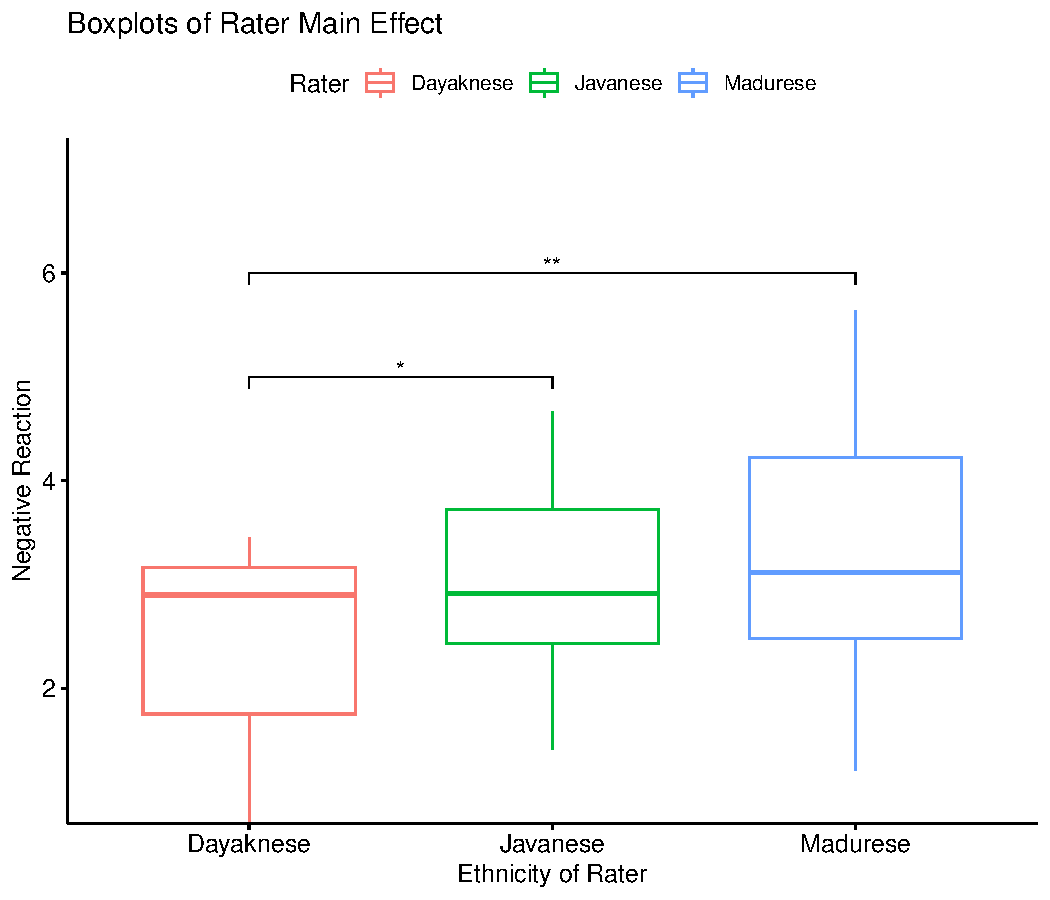
\includegraphics{07-OnewayANOVA_files/figure-latex/unnamed-chunk-58-1.pdf} In this particular research vignette, I probably would not compute nor report the non-orthogonal option. The statistically significant difference pattern from the post hoc pairwise comparisons (Option 1) was straightforward. Using the non-orthogonal planned comparisons to aid in the control of Type I error way (a) does not change the result (i.e., does not increase the power) and (b) provides a less complete picture of the results.

\hypertarget{option-3-orthogonal-planned-contrasts}{%
\subsubsection{OPTION \#3: Orthogonal planned contrasts}\label{option-3-orthogonal-planned-contrasts}}

\emph{Orthogonal} contrasts are even more sophisticated. Essential to conducting an orthogonal contrast is the requirement that if a group is singled out in one comparison it should be excluded from subsequent contrasts. The typical, orthogonal scenario with three ordered groups has only two contrasts:

\begin{enumerate}
\def\labelenumi{\arabic{enumi}.}
\tightlist
\item
  Control versus the combined low and high conditions
\end{enumerate}

\begin{itemize}
\tightlist
\item
  because control was excluded, it should not reappear in the next contrast
\end{itemize}

\begin{enumerate}
\def\labelenumi{\arabic{enumi}.}
\setcounter{enumi}{1}
\tightlist
\item
  Low versus high
\end{enumerate}

Especially in scenarios where there are no, low and high dose (or exposure) conditions, this is an elegant comparison. Unfortunately, at the time of this writing, the \emph{rstatix} package does not offer a function to make these computations. We can, however, use functions from base R. Given that \emph{rstatix} is a wrapper for the \emph{aov()} function in base R, the code should feel somewhat familiar.

To work toward our orthogonal contrasts, we first need to create an object (``omnibus1w\_b'') from a one-way ANOVA test using the base R, \emph{aov()} function. You can see that the script involves the same elements as in \emph{rstatix}. We can view the results byusing the \emph{summary()} function.

\begin{Shaded}
\begin{Highlighting}[]
\NormalTok{omnibus1w\_b }\OtherTok{\textless{}{-}} \FunctionTok{aov}\NormalTok{(Accurate }\SpecialCharTok{\textasciitilde{}}\NormalTok{ COND, }\AttributeTok{data =}\NormalTok{ accSIM30)}
\FunctionTok{summary}\NormalTok{(omnibus1w\_b)}
\end{Highlighting}
\end{Shaded}

\begin{verbatim}
            Df Sum Sq Mean Sq F value     Pr(>F)    
COND         2  9.432   4.716   13.57 0.00000745 ***
Residuals   87 30.246   0.348                       
---
Signif. codes:  0 '***' 0.001 '**' 0.01 '*' 0.05 '.' 0.1 ' ' 1
\end{verbatim}

This foray into orthogonal contrasts gives us a peek into multiple regression. Let's take a peek at ``regression results'' from our ANOVA model.

\begin{Shaded}
\begin{Highlighting}[]
\FunctionTok{summary.lm}\NormalTok{(omnibus1w\_b)}
\end{Highlighting}
\end{Shaded}

\begin{verbatim}

Call:
aov(formula = Accurate ~ COND, data = accSIM30)

Residuals:
     Min       1Q   Median       3Q      Max 
-1.24533 -0.32092  0.08642  0.30101  1.51646 

Coefficients:
            Estimate Std. Error t value             Pr(>|t|)    
(Intercept)   1.7562     0.1076  16.314 < 0.0000000000000002 ***
CONDLow       0.1439     0.1522   0.945             0.347095    
CONDHigh     -0.6034     0.1522  -3.963             0.000151 ***
---
Signif. codes:  0 '***' 0.001 '**' 0.01 '*' 0.05 '.' 0.1 ' ' 1

Residual standard error: 0.5896 on 87 degrees of freedom
Multiple R-squared:  0.2377,    Adjusted R-squared:  0.2202 
F-statistic: 13.57 on 2 and 87 DF,  p-value: 0.000007446
\end{verbatim}

The values on the row labeled \emph{intercept} are the values of the baseline or comparison group. Since CONDLow and CONDHigh follow, we know the three groups are sensibly ordered as control (0), low (1), and high (2).

While we are here, we observe that the control mean is 1.76 and that this value is statistically significantly different than zero. The \emph{CONDLow} row represents the low level of the condition variable. The mean for ``low'' is 0.14 units bigger than the control group and this is not a statistically significant difference (\(p = 0.347\)). The third row is the high level of the condition variable. This value is 0.60 units lower than the control condition and is statistically significantly different than zero (\(p < .001\)). This information is consistent with what we have already learned.

To move forward with the orthogonal contrasts we must first specify our contrasts.

\begin{itemize}
\tightlist
\item
  Specifying the contrasts means you know their order within the factor
\item
  Early in the data preparation, we created an ordered factor with Control, Low, High as the order.
\item
  We want orthogonal contrasts, this means there will be

  \begin{itemize}
  \tightlist
  \item
    \emph{k} - 1 contrasts; with three groups we will have two contrasts
  \item
    once we single out a condition for comparison, we cannot use it again.
  \end{itemize}
\end{itemize}

In \emph{contrast1} we compare the control condition to the combined low and high conditions. In \emph{contrast2} we discard the control condition (it was already singled out) and we compare the low and high conditions.

This is sensible because we likely hypothesize that any degree of racially loaded stereotypes may have a deleterious outcome, so we first compare control to the two conditions with any degree of racial loading. Subsequently, we compare the low and high levels of the factor.

In the second step we must bind the contrasts together and check the output to ensure that we've mapped them correctly.

\begin{Shaded}
\begin{Highlighting}[]
\CommentTok{\# Contrast1 compares Control against the combined effects of Low and}
\CommentTok{\# High.}
\NormalTok{contrast1 }\OtherTok{\textless{}{-}} \FunctionTok{c}\NormalTok{(}\SpecialCharTok{{-}}\DecValTok{2}\NormalTok{, }\DecValTok{1}\NormalTok{, }\DecValTok{1}\NormalTok{)}

\CommentTok{\# Contrast2 excludes Control; compares Low to High.}
\NormalTok{contrast2 }\OtherTok{\textless{}{-}} \FunctionTok{c}\NormalTok{(}\DecValTok{0}\NormalTok{, }\SpecialCharTok{{-}}\DecValTok{1}\NormalTok{, }\DecValTok{1}\NormalTok{)}

\CommentTok{\# binding the contrasts together}
\FunctionTok{contrasts}\NormalTok{(accSIM30}\SpecialCharTok{$}\NormalTok{COND) }\OtherTok{\textless{}{-}} \FunctionTok{cbind}\NormalTok{(contrast1, contrast2)}
\NormalTok{accSIM30}\SpecialCharTok{$}\NormalTok{COND}
\end{Highlighting}
\end{Shaded}

\begin{verbatim}
 [1] High    High    High    High    High    High    High    High    High   
[10] High    High    High    High    High    High    High    High    High   
[19] High    High    High    High    High    High    High    High    High   
[28] High    High    High    Low     Low     Low     Low     Low     Low    
[37] Low     Low     Low     Low     Low     Low     Low     Low     Low    
[46] Low     Low     Low     Low     Low     Low     Low     Low     Low    
[55] Low     Low     Low     Low     Low     Low     Control Control Control
[64] Control Control Control Control Control Control Control Control Control
[73] Control Control Control Control Control Control Control Control Control
[82] Control Control Control Control Control Control Control Control Control
attr(,"contrasts")
        contrast1 contrast2
Control        -2         0
Low             1        -1
High            1         1
Levels: Control Low High
\end{verbatim}

Thinking back to the hand-calculations and contrast mapping, the table of weights that R just produced confirms that

\begin{itemize}
\tightlist
\item
  Contrast 1 compares the Control condition against the levels with any racial loading.\\
\item
  Contrast 2 compares the Low and High loadings.
\end{itemize}

Finally, we create a new \emph{aov()} model and apply the contrasts.

\begin{Shaded}
\begin{Highlighting}[]
\CommentTok{\# create a new objects}
\NormalTok{accPlanned }\OtherTok{\textless{}{-}} \FunctionTok{aov}\NormalTok{(Accurate }\SpecialCharTok{\textasciitilde{}}\NormalTok{ COND, }\AttributeTok{data =}\NormalTok{ accSIM30)}
\FunctionTok{summary.lm}\NormalTok{(accPlanned)}
\end{Highlighting}
\end{Shaded}

\begin{verbatim}

Call:
aov(formula = Accurate ~ COND, data = accSIM30)

Residuals:
     Min       1Q   Median       3Q      Max 
-1.24533 -0.32092  0.08642  0.30101  1.51646 

Coefficients:
              Estimate Std. Error t value             Pr(>|t|)    
(Intercept)    1.60304    0.06215  25.793 < 0.0000000000000002 ***
CONDcontrast1 -0.07658    0.04395  -1.742                0.085 .  
CONDcontrast2 -0.37365    0.07612  -4.909           0.00000425 ***
---
Signif. codes:  0 '***' 0.001 '**' 0.01 '*' 0.05 '.' 0.1 ' ' 1

Residual standard error: 0.5896 on 87 degrees of freedom
Multiple R-squared:  0.2377,    Adjusted R-squared:  0.2202 
F-statistic: 13.57 on 2 and 87 DF,  p-value: 0.000007446
\end{verbatim}

These planned contrasts show that when the control condition is compared to the combined low and high racial loading conditions, there is not a statistically significant difference, \emph{t}(87) = -1.742, \emph{p} = 0.085. However, when the low and high racial loading conditions are compared, there is a statistically significant difference, \emph{t}(87) = -4.909, \emph{p} \textless{} 0.001. An APA style results write-up might look like this:

\begin{quote}
We followed the significant omnibus test with a pair of orthogonal contrasts. The first compared the control condition to the combined low and high racial loading conditions. The result was non-significant (\(t[87] = -1.742, p = 0.085\)). The second contrast compared the low and high racial loading conditions. In this contrast, accuracy ratings were statistically significantly lower for the high racial loading condition (\(t[87] = -4.909, p < 0.001\)).
\end{quote}

At this point, I do not have script that would update the \emph{ggpubr} graph with these results. If I were to use this follow-up in my APA style results, I would likely use the boxplot we produced at the beginning of the lesson.

\hypertarget{option-4-trend-polynomial-analysis}{%
\subsubsection{OPTION \#4: Trend (polynomial) analysis}\label{option-4-trend-polynomial-analysis}}

Polynomial contrasts let us see if there is a linear (or curvilinear) pattern to the data. To detect a trend, the data must be coded in an ascending order\ldots and it needs to be a sensible comparison. Here's where this would fall in our workflow.

\begin{figure}
\centering
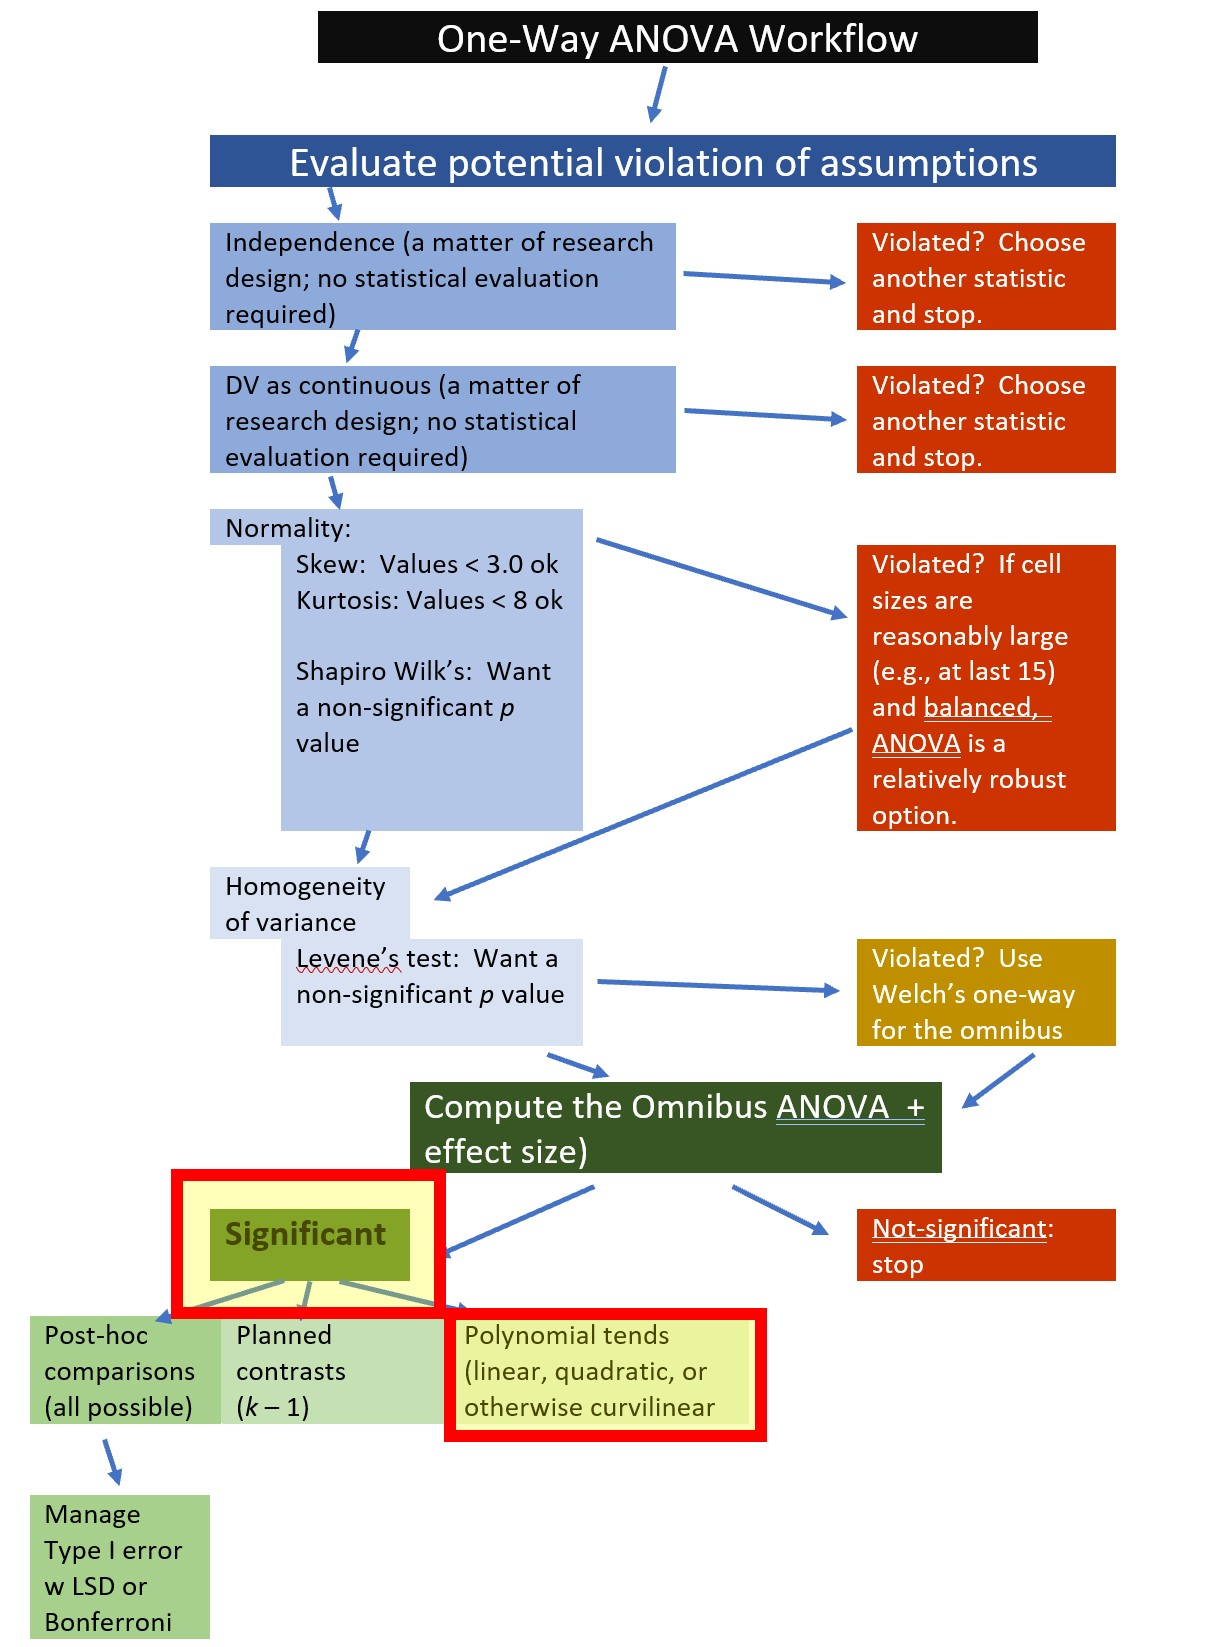
\includegraphics{images/oneway/OnewayWrkFlw_poly.jpg}
\caption{An image of the workflow for one-way ANOVA, showing that we are at the following up to a significant omnibus F by assessing for a polynomial trend}
\end{figure}

To detect a trend, the data must be coded in an ascending order and the comparison needs to be sensible and theoretically defensible. Our data has a theoretically ordered effect (control/none, low, and high racially loaded conditions). Recall that we created an ordered factor when we imported the data. However, we can use use the \emph{contrasts()} function from base R to verify the order.

\begin{Shaded}
\begin{Highlighting}[]
\FunctionTok{contrasts}\NormalTok{(accSIM30}\SpecialCharTok{$}\NormalTok{COND)}
\end{Highlighting}
\end{Shaded}

\begin{verbatim}
        contrast1 contrast2
Control        -2         0
Low             1        -1
High            1         1
\end{verbatim}

In a polynomial analysis, the statistical analysis looks across the ordered means to see if they fit a linear or curvilinear shape that is one fewer than the number of levels (i.e., \(k-1\)). Because the COND factor has three levels, the polynomial contrast checks for linear (.L) and quadratic (one change in direction) trends (.Q). If we had four levels, \emph{contr.poly()} could also check for cubic change (two changes in direction). Conventionally, when more than one trend is significant, we interpret the most complex one (i.e., quadratic over linear).

To the best of my knowledge, \emph{rstatix} does not offer these contrasts. We can fairly easily make these calculations in base R by creating a set of polynomial contrasts. In the prior example we specified our contrasts through coding. Here we can the \emph{contr.poly(3)} function. The ``3'' lets R know that there are three levels in COND. The \emph{aov()} function will automatically test for quadratic (one hump) and linear (straight line) trends.

\begin{Shaded}
\begin{Highlighting}[]
\FunctionTok{contrasts}\NormalTok{(accSIM30}\SpecialCharTok{$}\NormalTok{COND) }\OtherTok{\textless{}{-}} \FunctionTok{contr.poly}\NormalTok{(}\DecValTok{3}\NormalTok{)}
\NormalTok{accTrend }\OtherTok{\textless{}{-}} \FunctionTok{aov}\NormalTok{(Accurate }\SpecialCharTok{\textasciitilde{}}\NormalTok{ COND, }\AttributeTok{data =}\NormalTok{ accSIM30)}
\FunctionTok{summary.lm}\NormalTok{(accTrend)}
\end{Highlighting}
\end{Shaded}

\begin{verbatim}

Call:
aov(formula = Accurate ~ COND, data = accSIM30)

Residuals:
     Min       1Q   Median       3Q      Max 
-1.24533 -0.32092  0.08642  0.30101  1.51646 

Coefficients:
            Estimate Std. Error t value             Pr(>|t|)    
(Intercept)  1.60304    0.06215  25.793 < 0.0000000000000002 ***
COND.L      -0.42665    0.10765  -3.963             0.000151 ***
COND.Q      -0.36384    0.10765  -3.380             0.001087 ** 
---
Signif. codes:  0 '***' 0.001 '**' 0.01 '*' 0.05 '.' 0.1 ' ' 1

Residual standard error: 0.5896 on 87 degrees of freedom
Multiple R-squared:  0.2377,    Adjusted R-squared:  0.2202 
F-statistic: 13.57 on 2 and 87 DF,  p-value: 0.000007446
\end{verbatim}

Results of our polynomial contrast suggested statistically significant results for both linear \(t(87) = -3.963 , p < .001\) and quadratic \(t(87) = -3.380, p = .001\) trends. A quick peek back at any of our boxplots illustrates the quadratic trend (an small increase in accuracy from control to low; a larger decrease in accuracy from low to high) that was supported by this analysis.

Given that our earlier analyses did not support statistically significant differences between control and low racial loading conditions, I am disinclined to include this information. That said, there are times when I will include results of a polynomial trend along with the results of posthoc or planned pairwise comparisons. I will do this when the overall trend in the data helps clarify the results. For example, if in a circumstance where there was a clear linear trend between no, low, and high dose conditions and the pairwise results were consistent with that (i.e., statistically significant differences between no and low, no and high, low and high), I would likely add the results of the polynomial, after presenting the results of the posthoc or planned comparisons:

\begin{quote}
Additionally, results of a polynomial constrasted suggested a statistically significant linear trend across the three conditions, \(t(87) = -3.963 , p < .001\).
\end{quote}

At this point, I do not have script that would update the \emph{ggpubr} figure in a manner that would clearly convey these results. If I were to use this follow-up in my APA style results, I would likely use the simple boxplot we produced at the beginning of the lesson.

\hypertarget{which-set-of-follow-up-tests-do-we-report}{%
\subsubsection{Which set of follow-up tests do we report?}\label{which-set-of-follow-up-tests-do-we-report}}

It depends! Here are some things to consider.

\begin{itemize}
\tightlist
\item
  If the post hoc comparisons are robustly statistically significant (and controlling Type I error is not going to change that significance), I would lean toward reporting those.
\item
  If \emph{p} values are hovering around 0.05, an orthogonal contrast will offer more power because

  \begin{itemize}
  \tightlist
  \item
    a \emph{k} - 1 comparison will be more powerful and
  \item
    (when the research design allows) the contrast of no dose/exposure to any exposure followed by a contrast between low and high doses/exposures is compelling.
  \end{itemize}
\item
  The polynomial can be a useful descriptive addition if there is a linear or quadratic relationship that is sensible or interesting.
\end{itemize}

Although I would report either the post hoc or planned contrasts, I will sometimes add a polynomial if it clarifies the result (i.e., there is a meaningful linear or curvilinear pattern essential to understanding the data).

\hypertarget{what-if-we-violated-the-homogeneity-of-variance-test}{%
\subsection{What if we Violated the Homogeneity of Variance test?}\label{what-if-we-violated-the-homogeneity-of-variance-test}}

The \emph{rstatix::welch\_anova\_test} produces Welch's \emph{F} -- a test that is robust to violation of the homogeneity of variance assumption. The Welch's approach adjusts the residual degrees of freedom used to produce the Welch's \emph{F}-ratio. The format of the argument is quite similar to what we have been doing all along.

\begin{Shaded}
\begin{Highlighting}[]
\NormalTok{omnibus\_w }\OtherTok{\textless{}{-}}\NormalTok{ rstatix}\SpecialCharTok{::}\FunctionTok{welch\_anova\_test}\NormalTok{(accSIM30, Accurate }\SpecialCharTok{\textasciitilde{}}\NormalTok{ COND)}
\NormalTok{omnibus\_w}
\end{Highlighting}
\end{Shaded}

\begin{verbatim}
# A tibble: 1 x 7
  .y.          n statistic   DFn   DFd         p method     
* <chr>    <int>     <dbl> <dbl> <dbl>     <dbl> <chr>      
1 Accurate    90      11.6     2  56.3 0.0000617 Welch ANOVA
\end{verbatim}

Note that the denominator \emph{df} is now 56.34 (not 87) and \emph{p} value is a little larger (it was 0.00000745). With its design intended to avoid making a Type I error, the Welch's \emph{F} is more restrictive. While it wouldn't alter the conclusions in our research vignette, it could if the \emph{p} value was closer to 0.05. These are some of the tradeoffs we must consider in order to have confidence in the results. At this time the \emph{rstatix::welch\_anova\_test()} function does not offer an effect size. The omega squared is an effect size that is commonly reported with the Welch's \emph{F}. It would either need to be calculated by hand or with another R package.

In terms of follow-up to the omnibus test, \emph{rstatix} includes Games-Howell pairwise comparisons and pairwise t-tests. Neither of these follow-up options requires the assumption of equal variance. Consequently either could be used as a follow-up. Here's an example from the Games-Howell test.

\begin{Shaded}
\begin{Highlighting}[]
\NormalTok{gw\_pwc }\OtherTok{\textless{}{-}}\NormalTok{ rstatix}\SpecialCharTok{::}\FunctionTok{games\_howell\_test}\NormalTok{(accSIM30, Accurate }\SpecialCharTok{\textasciitilde{}}\NormalTok{ COND, }\AttributeTok{conf.level =} \FloatTok{0.95}\NormalTok{,}
    \AttributeTok{detailed =} \ConstantTok{TRUE}\NormalTok{)}
\NormalTok{gw\_pwc}
\end{Highlighting}
\end{Shaded}

\begin{verbatim}
# A tibble: 3 x 14
  .y.      group1 group2    n1    n2 estimate conf.low conf.high    se statistic
* <chr>    <chr>  <chr>  <int> <int>    <dbl>    <dbl>     <dbl> <dbl>     <dbl>
1 Accurate Contr~ Low       30    30    0.144   -0.200     0.487 0.101      1.01
2 Accurate Contr~ High      30    30   -0.603   -0.957    -0.249 0.104      4.11
3 Accurate Low    High      30    30   -0.747   -1.15     -0.347 0.118      4.49
# i 4 more variables: df <dbl>, p.adj <dbl>, p.adj.signif <chr>, method <chr>
\end{verbatim}

Another common correction for evaluating the omnibus test when there is a violation of the homogeneity of variance assumption is the Brown and Forsythe \emph{F}-ratio. The \emph{rstatix} package does not include this option (but other packages do).

\hypertarget{apa-style-results-3}{%
\section{APA Style Results}\label{apa-style-results-3}}

All that's left to do to decide which set of follow-up tests to report and assemble the write-up. APA style results sections in empirical manuscripts are typically accompanied by tables and figures. APA style discourages redundancy in information (i.e., if information is clearly presented in a table, do not repeat it verbatim in written text) and encourages reducing the cognitive load of the reader. For this example, I suggest two tables -- (a) one with means and standard deviations the dependent variable (disaggregated by level)and (b) a second that reports the output from the one-way ANOVA.

The package \emph{apaTables} can produce journal-ready tables. Deciding what to report in text and table is important. First, I create Table 1 with means and standard deviations (plus a 95\% confidence interval around each mean).

\begin{Shaded}
\begin{Highlighting}[]
\CommentTok{\# table.number = 1 assigns a table number to the top of the table}
\CommentTok{\# filename = \textquotesingle{}Table1.doc\textquotesingle{} writes the table to Microsoft Word and puts}
\CommentTok{\# it in your project folder}
\NormalTok{apaTables}\SpecialCharTok{::}\FunctionTok{apa.1way.table}\NormalTok{(}\AttributeTok{iv =}\NormalTok{ COND, }\AttributeTok{dv =}\NormalTok{ Accurate, }\AttributeTok{show.conf.interval =} \ConstantTok{TRUE}\NormalTok{,}
    \AttributeTok{data =}\NormalTok{ accSIM30, }\AttributeTok{table.number =} \DecValTok{1}\NormalTok{, }\AttributeTok{filename =} \StringTok{"Table1.doc"}\NormalTok{)}
\end{Highlighting}
\end{Shaded}

\begin{verbatim}


Table 1 

Descriptive statistics for Accurate as a function of COND.  

    COND    M     M_95%_CI   SD
 Control 1.76 [1.58, 1.93] 0.46
     Low 1.90 [1.66, 2.14] 0.63
    High 1.15 [0.91, 1.40] 0.66

Note. M and SD represent mean and standard deviation, respectively.
LL and UL indicate the lower and upper limits of the 95% confidence interval 
for the mean, respectively. 
The confidence interval is a plausible range of population means that could 
have caused a sample mean (Cumming, 2014). 
\end{verbatim}

Next, I create Table 2 with source table for the one-way ANOVA. The result can be edited in Microsoft Word for the paper or presentation (e.g., I would replace the partial-eta squared with \(\eta^2\)). One trick about \emph{apaTables::aov} is that it requires an object from the base R's \emph{aov} function. Recall that we used this in our contrasts. None-the-less, I will repeat it in this code.

\begin{Shaded}
\begin{Highlighting}[]
\NormalTok{omnibus1w\_b }\OtherTok{\textless{}{-}} \FunctionTok{aov}\NormalTok{(Accurate }\SpecialCharTok{\textasciitilde{}}\NormalTok{ COND, }\AttributeTok{data =}\NormalTok{ accSIM30)}
\NormalTok{apaTables}\SpecialCharTok{::}\FunctionTok{apa.aov.table}\NormalTok{(omnibus1w\_b, }\AttributeTok{table.number =} \DecValTok{2}\NormalTok{, }\AttributeTok{filename =} \StringTok{"Table2.doc"}\NormalTok{)}
\end{Highlighting}
\end{Shaded}

\begin{verbatim}


Table 2 

ANOVA results using Accurate as the dependent variable
 

   Predictor     SS df     MS      F    p partial_eta2 CI_90_partial_eta2
 (Intercept) 231.28  1 231.28 665.25 .000                                
        COND   9.43  2   4.71  13.57 .000          .24         [.11, .34]
       Error  30.25 87   0.35                                            

Note: Values in square brackets indicate the bounds of the 90% confidence interval for partial eta-squared 
\end{verbatim}

Regarding figures, I would use the one I created with the set of follow-up results.

With table and figure at hand, here is how I would write up these results:

\begin{quote}
A one-way analysis of variance was conducted to evaluate the relationship between degree of racial loading of an exceptionalizing microaggression and the perceived accuracy of a research confederate's impression of the Asian or Asian American participant. The independent variable, condition, included three levels: control/none, low, and high levels of racial loading.
\end{quote}

\begin{quote}
Regarding the assumption of normality, skew and kurtosis values at each of the levels of the condition value fell well below the thresholds that Kline \citeyearpar{kline_data_2016} identified as concerning (i.e., below \textbar3\textbar{} for skew and \textbar10\textbar{} for kurtosis). Similarly, no extreme outliers were identified and results of a model-based Shapiro-Wilk test of normality, indicated that the model residuals did not did differ from a normal distribution \((W = 0.979, p = 0.15)\). Finally, Levene's homogeneity of variance test indicated no violation of the homogeneity of variance assumption (\(F[2, 87] = 1.695, p = 0.190\)).
\end{quote}

\begin{quote}
Results of the omnibus ANOVA indicated a significant effect of COND on accuracy perception \((F[2,87] = 13.566, p < .001, \eta ^{2} = 0.238\)). We followed up the significant omnibus with a series of post hoc, pairwise comparisons. We controlled for Type I error with the traditional Bonferroni adjustment. Results suggested that there were statistically significant differences between the control and high (\(M_{diff} = 0.601, p < .001\)) and low and high (\(M_{diff} = 0.75, p < 0.001\)) conditions, but not control and low conditions (\(M_{diff} = -.14, p = 0.951\)). Consequently, it appeared that only the highest degree of racial loading (e.g., ``You speak English well for an Asian'') resulted in the decreased perceptions of accuracy of impressions from the confederate. Means and standard deviations are presented in Table 1 and complete ANOVA results are presented in Table 2. Figure 1 provides an illustration of the results.
\end{quote}

\begin{Shaded}
\begin{Highlighting}[]
\NormalTok{Fig1}
\end{Highlighting}
\end{Shaded}

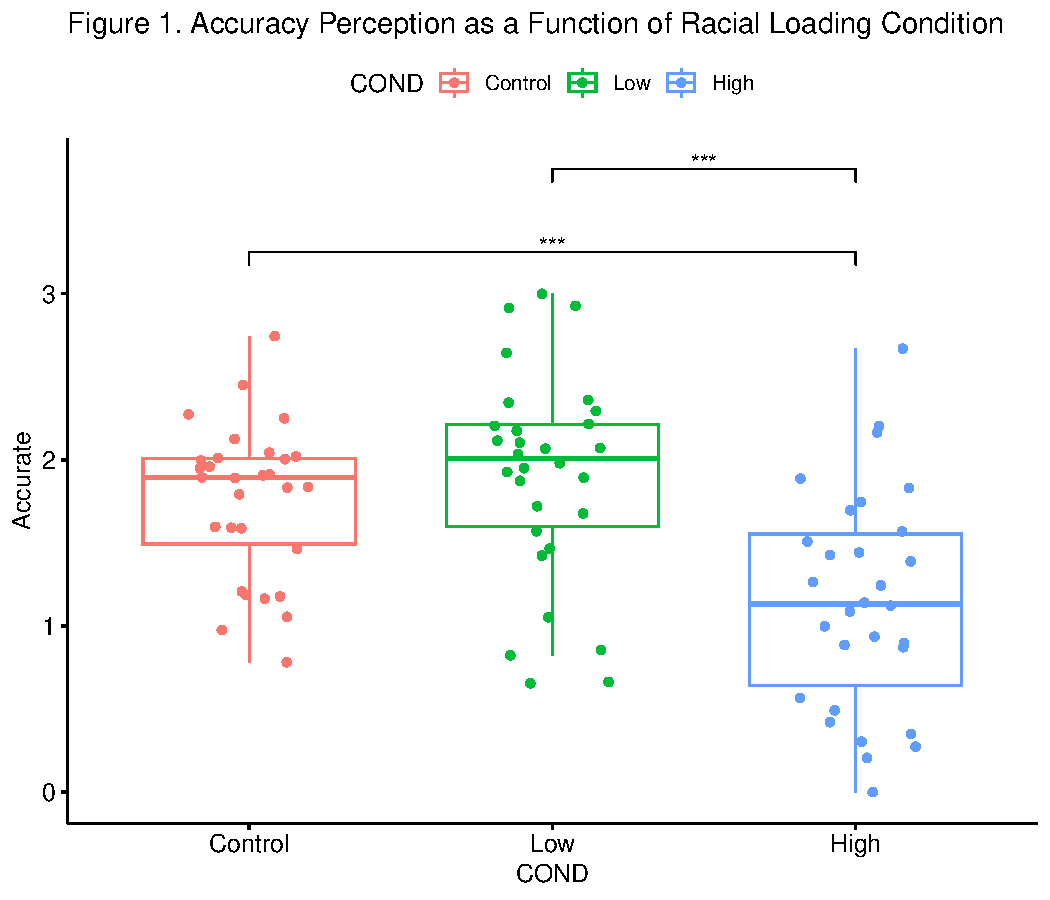
\includegraphics{07-OnewayANOVA_files/figure-latex/unnamed-chunk-69-1.pdf}

\hypertarget{power-analysis}{%
\section{Power Analysis}\label{power-analysis}}

Power analysis allows us to determine the sample size required to detect an effect of a given size with a given degree of confidence. Utilized another way, it allows us to determine the probability of detecting an effect of a given size with a given level of confidence. If the probability is unacceptably low, we may want to revise or stop. A helpful overview of power as well as guidelines for how to use the \emph{pwr} package can be found at a \href{https://www.statmethods.net/stats/power.html}{Quick-R website} \citep{kabacoff_power_2017}.

There are four interrelating elements of power:

\begin{enumerate}
\def\labelenumi{\arabic{enumi}.}
\tightlist
\item
  Sample size, \emph{N}
\item
  Effect size,

  \begin{itemize}
  \tightlist
  \item
    For one-way ANOVAs, Cohen suggests that f values of 0.1, 0.25, and 0.4 represent small, medium, and large effect sizes, respectively.
  \end{itemize}
\item
  Significance level = P(Type I error),

  \begin{itemize}
  \tightlist
  \item
    Recall that Type I error is the rejection of a true null hypothesis (a false positive).
  \item
    Stated another way, Type I error is the probability of finding an effect that is not there.
  \end{itemize}
\item
  Power = 1 - P(Type II error),

  \begin{itemize}
  \tightlist
  \item
    Recall that Type II error is the non-rejection of a false null hypothesis (a false negative).
  \item
    Power is the probability of finding an effect that is there.
  \end{itemize}
\end{enumerate}

If we have any three of these values, we can calculate the fourth.

In Champely's \emph{pwr} package, we can conduct a power analysis for a variety of designs, including the balanced one-way ANOVA (i.e., roughly equal cell sizes) design that we worked in this chapter.

The \emph{pwr.anova.test()} has five parameters:

\begin{itemize}
\tightlist
\item
  \emph{k} = \# groups
\item
  \emph{n} = sample size
\item
  \emph{f} = effect sizes, where 0.1/small, 0.25/medium, and 0.4/large

  \begin{itemize}
  \tightlist
  \item
    In the absence from an estimate from our own data, we make a guess about the expected effect size value based on our knowledge of the literature
  \end{itemize}
\item
  \emph{sig.level} = \emph{p} value that you will use
\item
  \emph{power} = .80 is the standard value
\end{itemize}

In the script below, we simply add our values. So long as we have four values, the fifth will be calculated for us.

Because this calculator requires the effect size in the metric of Cohen's \emph{f} (this is not the same as the \emph{F} ratio), we need to convert it. The \emph{effectsize} package has a series of converters. We can use the \emph{eta2\_to\_f()} function.

\begin{Shaded}
\begin{Highlighting}[]
\NormalTok{effectsize}\SpecialCharTok{::}\FunctionTok{eta2\_to\_f}\NormalTok{(}\FloatTok{0.238}\NormalTok{)}
\end{Highlighting}
\end{Shaded}

\begin{verbatim}
[1] 0.5588703
\end{verbatim}

We simply plug this value into the ``f =''.

\begin{Shaded}
\begin{Highlighting}[]
\NormalTok{pwr}\SpecialCharTok{::}\FunctionTok{pwr.anova.test}\NormalTok{(}\AttributeTok{k =} \DecValTok{3}\NormalTok{, }\AttributeTok{f =} \FloatTok{0.5589}\NormalTok{, }\AttributeTok{sig.level =} \FloatTok{0.05}\NormalTok{, }\AttributeTok{power =} \FloatTok{0.8}\NormalTok{)}
\end{Highlighting}
\end{Shaded}

\begin{verbatim}

     Balanced one-way analysis of variance power calculation 

              k = 3
              n = 11.3421
              f = 0.5589
      sig.level = 0.05
          power = 0.8

NOTE: n is number in each group
\end{verbatim}

This result suggested that we would need 11 people per group.

If we were unsure about what to expect in terms of our results, we could take a guess. I like to be on the safe(r) side and go with a smaller effect. What would happen if we had a Cohen's \emph{f} that represented a small effect?

\begin{Shaded}
\begin{Highlighting}[]
\NormalTok{pwr}\SpecialCharTok{::}\FunctionTok{pwr.anova.test}\NormalTok{(}\AttributeTok{k =} \DecValTok{3}\NormalTok{, }\AttributeTok{f =} \FloatTok{0.1}\NormalTok{, }\AttributeTok{sig.level =} \FloatTok{0.05}\NormalTok{, }\AttributeTok{power =} \FloatTok{0.8}\NormalTok{)}
\end{Highlighting}
\end{Shaded}

\begin{verbatim}

     Balanced one-way analysis of variance power calculation 

              k = 3
              n = 322.157
              f = 0.1
      sig.level = 0.05
          power = 0.8

NOTE: n is number in each group
\end{verbatim}

Yikes! We would need over 300 per group!

If effect sizes are new to you, play around with this effect size converter hosted at \href{https://www.psychometrica.de/effect_size.html}{Psychometrica.de}. For examples like this one, use the option labeled, ``Transformation of the effect sizes \emph{d}, \emph{r}, \emph{f}, \emph{Odds Ratio}, \(\eta^2\), and \emph{Common Language Effect Size (CLES}).''

\hypertarget{a-conversation-with-dr.-tran}{%
\section{A Conversation with Dr.~Tran}\label{a-conversation-with-dr.-tran}}

Doctoral student (and student in one of my classes) Emi Ichimura and I were able to interview the first author (Alisia Tran, PhD) about the article and what it means. Here's a direct \href{https://spu.hosted.panopto.com/Panopto/Pages/Viewer.aspx?id=643f8a1e-bb6d-4ceb-a860-aeba01522528}{link} to that interview.

Among others, we asked:

\begin{itemize}
\tightlist
\item
  What were unexpected challenges to the research method or statistical analysis?
\item
  What were the experiences of the confederates as they offered the statements in teh racial loading conditions? And in the debriefings, did the research participants share anything more anecdotally in their experiences as research participants?
\item
  What are your current ideas about interventions or methods for mitigating the harm caused by racial microaggressions?
\item
  How do you expect the article to change science, practice, and/or advocacy?
\end{itemize}

\hypertarget{practice-problems-5}{%
\section{Practice Problems}\label{practice-problems-5}}

The suggestions for homework differ in degree of complexity. I encourage you to start with a problem that feels ``do-able'' and then try at least one more problem that challenges you in some way. The data for each vignette should have at least three levels in the independent variable. Further, at least one of the problems you work should have a significant omnibus test so that follow-up is required.

Regardless, your choices should meet you where you are (e.g., in terms of your self-efficacy for statistics, your learning goals, and competing life demands). Whichever you choose, you will focus on these larger steps in one-way ANOVA, including:

\begin{itemize}
\tightlist
\item
  testing the statistical assumptions
\item
  conducting a one-way ANOVA, including

  \begin{itemize}
  \tightlist
  \item
    omnibus test and effect size
  \item
    follow-up (pairwise, planned comparisons, polynomial trends)
  \end{itemize}
\item
  writing a results section to include a figure and tables
\end{itemize}

Additionally, please complete at least one set of \emph{hand calculations}, that is use the code demonstrated in the chapter to work through the formulas that compute the one-way ANOVA. At this stage in your learning, you may ignore any missingness in your dataset by excluding all rows with missing data in your variables of interest.

\hypertarget{problem-1-play-around-with-this-simulation.}{%
\subsection{Problem \#1: Play around with this simulation.}\label{problem-1-play-around-with-this-simulation.}}

If one-way ANOVA is new to you, perhaps you just change the number in ``set.seed(2021)'' from 2021 to something else. Your results should parallel those obtained in the lecture, making it easier for you to check your work as you go.

There are other ways to change the dataset. For example, if you are interested in power, change the sample size to something larger or smaller. If you are interested in variability (i.e., the homogeneity of variance assumption), perhaps you change the standard deviations in a way that violates the assumption.

\hypertarget{problem-2-conduct-a-one-way-anova-with-the-moretalk-dependent-variable.}{%
\subsection{\texorpdfstring{Problem \#2: Conduct a one-way ANOVA with the \emph{moreTalk} dependent variable.}{Problem \#2: Conduct a one-way ANOVA with the moreTalk dependent variable.}}\label{problem-2-conduct-a-one-way-anova-with-the-moretalk-dependent-variable.}}

In their study, Tran and Lee \citeyearpar{tran_you_2014} included an outcome variable where participants rated how much longer they would continue the interaction with their partner compared to their interactions in general. The scale ranged from -2 (\emph{much less than average}) through 0 (\emph{average}) to 2 (\emph{much more than average}). This variable is available in the original simulation and is an option for a slightly more challenging analysis.

\hypertarget{problem-3-try-something-entirely-new.}{%
\subsection{Problem \#3: Try something entirely new.}\label{problem-3-try-something-entirely-new.}}

Using data for which you have permission and access (e.g., IRB approved data you have collected or from your lab; data you simulate from a published article; data from an open science repository; data from other chapters in this OER), complete a one-way ANOVA. Please have at least 3 levels for the predictor variable.

\hypertarget{grading-rubric-3}{%
\subsection{Grading Rubric}\label{grading-rubric-3}}

Regardless which option(s) you chose, use the elements in the grading rubric to guide you through the practice.

\begin{longtable}[]{@{}
  >{\raggedright\arraybackslash}p{(\columnwidth - 4\tabcolsep) * \real{0.5493}}
  >{\centering\arraybackslash}p{(\columnwidth - 4\tabcolsep) * \real{0.2535}}
  >{\centering\arraybackslash}p{(\columnwidth - 4\tabcolsep) * \real{0.1972}}@{}}
\toprule\noalign{}
\begin{minipage}[b]{\linewidth}\raggedright
Assignment Component
\end{minipage} & \begin{minipage}[b]{\linewidth}\centering
Points Possible
\end{minipage} & \begin{minipage}[b]{\linewidth}\centering
Points Earned
\end{minipage} \\
\midrule\noalign{}
\endhead
\bottomrule\noalign{}
\endlastfoot
1. Narrate the research vignette, describing the IV and DV. The data you analyze should have at least 3 levels in the independent variable; at least one of the attempted problems should have a significant omnibus test so that follow-up is required). & 5 & \_\_\_\_\_ \\
2. Simulate (or import) and format data. & 5 & \_\_\_\_\_ \\
3. Evaluate statistical assumptions. & 5 & \_\_\_\_\_ \\
4. Conduct omnibus ANOVA (w effect size). & 5 & \_\_\_\_\_ \\
5. Conduct one set of follow-up tests; narrate your choice. & 5 & \_\_\_\_\_ \\
6. Describe approach for managing Type I error. & 5 & \_\_\_\_\_ \\
7. APA style results with table(s) and figure. & 5 & \_\_\_\_\_ \\
8. Conduct power analyses to determine the power of the current study and a recommended sample size. & 5 & \_\_\_\_\_ \\
9. Explanation to grader. & 5 & \_\_\_\_\_ \\
\textbf{Totals} & 40 & \_\_\_\_\_ \\
\end{longtable}

\begin{longtable}[]{@{}
  >{\raggedright\arraybackslash}p{(\columnwidth - 4\tabcolsep) * \real{0.5833}}
  >{\centering\arraybackslash}p{(\columnwidth - 4\tabcolsep) * \real{0.2083}}
  >{\raggedright\arraybackslash}p{(\columnwidth - 4\tabcolsep) * \real{0.2083}}@{}}
\toprule\noalign{}
\begin{minipage}[b]{\linewidth}\raggedright
Hand Calculations
\end{minipage} & \begin{minipage}[b]{\linewidth}\centering
Points Poss
\end{minipage} & \begin{minipage}[b]{\linewidth}\raggedright
Points Earned
\end{minipage} \\
\midrule\noalign{}
\endhead
\bottomrule\noalign{}
\endlastfoot
1. Using traditional NHST (null hypothesis testing language), state your null and alternative hypotheses. & 2 & \\
2. Calculate sums of squares total (SST). Steps in this calculation must include calculating a grand mean and creating variables representing the mean deviation and mean deviation squared. & 4 & \\
3. Calculate the sums of squares for the model (SSM). A necessary step in this equation is to calculate group means. & 4 & \\
4. Calculate the sums of squares residual (SSR). A necessary step in this equation is to calculate the variance for each group. & 4 & \\
5. Calculate the mean square model, mean square residual, and \emph{F}-test. & 2 & \\
6. What are the degrees of freedom for your numerator and denominator? & 2 & \\
7. Locate the test critical value for your one-way ANOVA. & 2 & \\
8. Is the \emph{F}-test statistically significant? Why or why not? & 2 & \\
9. Calculate and interpret the \(\eta^2\) effect size & 2 & \\
\end{longtable}

\textbar10. Assemble the results into a statistical string. \textbar4 \textbar{} \textbar{} \textbar{}\textbf{Totals* } \textbar{} 28 \textbar{} \textbar{}

\hypertarget{homeworked-example-5}{%
\section{Homeworked Example}\label{homeworked-example-5}}

\href{}{Screencast Link}

\emph{If you wanted to use this example and dataset as a basis for a homework assignment, you could create a different subset of data. I worked the example for students taking the ANOVA class. You could choose multivariate or psychometrics. You could also choose a different dependent variable. I chose the traditional pedagogy subscale. Two other subscales include socially responsive pedagogy and valued by the student.}

\hypertarget{working-the-problem-with-r-and-r-packages-4}{%
\subsection{Working the Problem with R and R Packages}\label{working-the-problem-with-r-and-r-packages-4}}

\hypertarget{narrate-the-research-vignette-describing-the-iv-and-dv.-the-data-you-analyze-should-have-at-least-3-levels-in-the-independent-variable-at-least-one-of-the-attempted-problems-should-have-a-significant-omnibus-test-so-that-follow-up-is-required.}{%
\subsubsection{Narrate the research vignette, describing the IV and DV. The data you analyze should have at least 3 levels in the independent variable; at least one of the attempted problems should have a significant omnibus test so that follow-up is required).}\label{narrate-the-research-vignette-describing-the-iv-and-dv.-the-data-you-analyze-should-have-at-least-3-levels-in-the-independent-variable-at-least-one-of-the-attempted-problems-should-have-a-significant-omnibus-test-so-that-follow-up-is-required.}}

I want to ask the question, do course evaluation ratings for traditional pedagogy differ for students as we enacted a substantive revision to our statistics series. The evaluative focus is on the ANOVA course and we will compare ratings from the stable, transition, and resettled stages of the transitional period. The variable (Stage) of interest will have three levels:

\begin{itemize}
\tightlist
\item
  STABLE: 2017 represents the last year of ``stability during the old way'' when we taught with SPSS and during the 2nd year of the doctoral programs.
\item
  TRANSITION: 2018 \& 2019 represent the transition to R, when the classes were 30\% larger because each of the IOP and CPY departments were transitioning to the 1st year (they did it separately, so as not to double the classes)
\item
  RESETTLED: 2020 \& 2021 represent the ``resettled'' phase where the transition to R was fairly complete and the class size returned to normal because the classes were offered in the first year.
\end{itemize}

This is not a variable that was included in the dataset posted to the OSF repository, so we will need to create it.

\hypertarget{simulate-or-import-and-format-data.}{%
\subsubsection{Simulate (or import) and format data.}\label{simulate-or-import-and-format-data.}}

\begin{Shaded}
\begin{Highlighting}[]
\NormalTok{big }\OtherTok{\textless{}{-}} \FunctionTok{readRDS}\NormalTok{(}\StringTok{"ReC.rds"}\NormalTok{)}
\end{Highlighting}
\end{Shaded}

This df includes course evaluations from ANOVA, multivariate, and psychometrics. To include up to three evaluations per student would violate the assumption of independence, therefore, I will only select the students in ANOVA course.

\begin{Shaded}
\begin{Highlighting}[]
\NormalTok{big }\OtherTok{\textless{}{-}} \FunctionTok{subset}\NormalTok{(big, Course }\SpecialCharTok{==} \StringTok{"ANOVA"}\NormalTok{) }
\end{Highlighting}
\end{Shaded}

Let's first create the ``Stage'' variable that represents the three levels of transition.

First I will map the years to the three levels (factors).

\begin{Shaded}
\begin{Highlighting}[]
\NormalTok{big}\SpecialCharTok{$}\NormalTok{Stage }\OtherTok{\textless{}{-}}\NormalTok{ plyr}\SpecialCharTok{::}\FunctionTok{mapvalues}\NormalTok{(big}\SpecialCharTok{$}\NormalTok{Year, }\AttributeTok{from =} \FunctionTok{c}\NormalTok{(}\DecValTok{2017}\NormalTok{, }\DecValTok{2018}\NormalTok{, }\DecValTok{2019}\NormalTok{, }\DecValTok{2020}\NormalTok{, }\DecValTok{2021}\NormalTok{), }\AttributeTok{to =} \FunctionTok{c}\NormalTok{(}\StringTok{"Stable"}\NormalTok{, }\StringTok{"Transition"}\NormalTok{, }\StringTok{"Transition"}\NormalTok{, }\StringTok{"Resettled"}\NormalTok{, }\StringTok{"Resettled"}\NormalTok{))}
\end{Highlighting}
\end{Shaded}

Then check the structure.

\begin{Shaded}
\begin{Highlighting}[]
\FunctionTok{str}\NormalTok{(big}\SpecialCharTok{$}\NormalTok{Stage)}
\end{Highlighting}
\end{Shaded}

\begin{verbatim}
 chr [1:114] "Resettled" "Resettled" "Resettled" "Resettled" "Resettled" ...
\end{verbatim}

R is reading the variable as a character, so I need to make it to be an ordered factor.

\begin{Shaded}
\begin{Highlighting}[]
\NormalTok{big}\SpecialCharTok{$}\NormalTok{Stage }\OtherTok{\textless{}{-}} \FunctionTok{factor}\NormalTok{(big}\SpecialCharTok{$}\NormalTok{Stage, }\AttributeTok{levels =} \FunctionTok{c}\NormalTok{(}\StringTok{"Stable"}\NormalTok{, }\StringTok{"Transition"}\NormalTok{, }\StringTok{"Resettled"}\NormalTok{))}
\end{Highlighting}
\end{Shaded}

Let's check the structure again:

\begin{Shaded}
\begin{Highlighting}[]
\FunctionTok{str}\NormalTok{(big}\SpecialCharTok{$}\NormalTok{Stage)}
\end{Highlighting}
\end{Shaded}

\begin{verbatim}
 Factor w/ 3 levels "Stable","Transition",..: 3 3 3 3 3 3 3 3 3 3 ...
\end{verbatim}

The TradPed (traditional pedagogy) variable is an average of the items on that scale. I will first create that variable.

\begin{Shaded}
\begin{Highlighting}[]
\CommentTok{\#Creates a list of the variables that belong to that scale}
\NormalTok{TradPed\_vars }\OtherTok{\textless{}{-}} \FunctionTok{c}\NormalTok{(}\StringTok{\textquotesingle{}ClearResponsibilities\textquotesingle{}}\NormalTok{, }\StringTok{\textquotesingle{}EffectiveAnswers\textquotesingle{}}\NormalTok{,}\StringTok{\textquotesingle{}Feedback\textquotesingle{}}\NormalTok{, }\StringTok{\textquotesingle{}ClearOrganization\textquotesingle{}}\NormalTok{,}\StringTok{\textquotesingle{}ClearPresentation\textquotesingle{}}\NormalTok{)}

\CommentTok{\#Calculates a mean if at least 75\% of the items are non{-}missing; adjusts the calculating when there is missingness}
\NormalTok{big}\SpecialCharTok{$}\NormalTok{TradPed }\OtherTok{\textless{}{-}}\NormalTok{ sjstats}\SpecialCharTok{::}\FunctionTok{mean\_n}\NormalTok{(big[, TradPed\_vars], .}\DecValTok{75}\NormalTok{)}
\end{Highlighting}
\end{Shaded}

With our variables properly formatted, let's trim it to just the variables we need.

\begin{Shaded}
\begin{Highlighting}[]
\NormalTok{OneWay\_df }\OtherTok{\textless{}{-}}\NormalTok{(dplyr}\SpecialCharTok{::}\FunctionTok{select}\NormalTok{ (big, Stage, TradPed))}
\end{Highlighting}
\end{Shaded}

Although we would handle missing data more carefully in a ``real study,'' I will delete all cases with any missingness. This will prevent problems in the hand-calculations section, later (and keep the two sets of results more similar).

\begin{Shaded}
\begin{Highlighting}[]
\NormalTok{df }\OtherTok{\textless{}{-}} \FunctionTok{na.omit}\NormalTok{(OneWay\_df)}
\end{Highlighting}
\end{Shaded}

\hypertarget{evaluate-statistical-assumptions.}{%
\subsubsection{Evaluate statistical assumptions.}\label{evaluate-statistical-assumptions.}}

\textbf{Is the dependent variable normally distributed across levels of the factor?}

\begin{Shaded}
\begin{Highlighting}[]
\NormalTok{psych}\SpecialCharTok{::}\FunctionTok{describeBy}\NormalTok{(TradPed }\SpecialCharTok{\textasciitilde{}}\NormalTok{ Stage, }\AttributeTok{mat =} \ConstantTok{TRUE}\NormalTok{, }\AttributeTok{digits =} \DecValTok{3}\NormalTok{, }\AttributeTok{data =}\NormalTok{ OneWay\_df, }\AttributeTok{type =} \DecValTok{1}\NormalTok{)}
\end{Highlighting}
\end{Shaded}

\begin{verbatim}
         item     group1 vars  n  mean    sd median trimmed   mad min max range
TradPed1    1     Stable    1 21 4.419 0.544    4.6   4.482 0.593 3.2   5   1.8
TradPed2    2 Transition    1 44 4.045 1.029    4.3   4.206 1.038 1.0   5   4.0
TradPed3    3  Resettled    1 47 3.909 0.778    4.0   3.967 0.890 1.8   5   3.2
           skew kurtosis    se
TradPed1 -0.623   -0.492 0.119
TradPed2 -1.312    1.177 0.155
TradPed3 -0.601   -0.041 0.113
\end{verbatim}

We'll use Kline's (2016) threshholds of the absolute values of 3 (skew) and 10 (kurtosis). The highest absolute value of skew is -1.31; the highest absolute value of kurtosis is 1.18. These are well below the areas of concern.

the Shapiro-wilk test is a formal assessment of normality. It is a 2-part test that begins with creating an ANOVA model from which we can extract residuals, then testing the residuals.

\begin{Shaded}
\begin{Highlighting}[]
\NormalTok{TradPed\_res }\OtherTok{\textless{}{-}} \FunctionTok{lm}\NormalTok{(TradPed }\SpecialCharTok{\textasciitilde{}}\NormalTok{ Stage, }\AttributeTok{data =}\NormalTok{ OneWay\_df)}
\NormalTok{rstatix}\SpecialCharTok{::}\FunctionTok{shapiro\_test}\NormalTok{(}\FunctionTok{residuals}\NormalTok{(TradPed\_res))}
\end{Highlighting}
\end{Shaded}

\begin{verbatim}
# A tibble: 1 x 3
  variable               statistic    p.value
  <chr>                      <dbl>      <dbl>
1 residuals(TradPed_res)     0.910 0.00000130
\end{verbatim}

The Shapiro-Wilk test suggests that the our distribution of residuals is statistically significantly different from a normal distribution \((W = 0.910, p < .001)\).

It is possible to plot the residuals to see how and where they deviate from the line.

\begin{Shaded}
\begin{Highlighting}[]
\NormalTok{ggpubr}\SpecialCharTok{::}\FunctionTok{ggqqplot}\NormalTok{(}\FunctionTok{residuals}\NormalTok{(TradPed\_res))}
\end{Highlighting}
\end{Shaded}

\includegraphics{07-OnewayANOVA_files/figure-latex/unnamed-chunk-86-1.pdf} Ooof! at the ends of the distribution they really deviate.

\textbf{Should we remove outliers?}

The \emph{rstatix::identify\_outliers()} function identifies outlers and extreme outliers.

\begin{Shaded}
\begin{Highlighting}[]
\FunctionTok{library}\NormalTok{(tidyverse)}
\NormalTok{OneWay\_df }\SpecialCharTok{\%\textgreater{}\%}
\NormalTok{  rstatix}\SpecialCharTok{::}\FunctionTok{identify\_outliers}\NormalTok{(TradPed)}
\end{Highlighting}
\end{Shaded}

\begin{verbatim}
       Stage TradPed is.outlier is.extreme
1  Resettled     1.8       TRUE      FALSE
2 Transition     1.0       TRUE      FALSE
3 Transition     1.4       TRUE      FALSE
4 Transition     1.6       TRUE      FALSE
\end{verbatim}

There are 4 cases identified with outliers; none of those is extreme. I also notice that these outliers are low course evaluations. It seems only fair to retain the data from individuals who were not satisfied with the course.

\textbf{Are the variances of the dependent variable similar across the levels of the grouping factor?}

We want the results of the Levene's homogeneity of variance test to be non-significant. This would support the notion that the TradPed variance is equivalent across the three stages of the transition.

\begin{Shaded}
\begin{Highlighting}[]
\NormalTok{rstatix}\SpecialCharTok{::}\FunctionTok{levene\_test}\NormalTok{(OneWay\_df, TradPed }\SpecialCharTok{\textasciitilde{}}\NormalTok{ Stage)}
\end{Highlighting}
\end{Shaded}

\begin{verbatim}
# A tibble: 1 x 4
    df1   df2 statistic     p
  <int> <int>     <dbl> <dbl>
1     2   109      2.09 0.128
\end{verbatim}

The non-significant \emph{p} value suggests that the variances across the three stages are not statistically significantly different: \(F(2, 109) = 2.094, p = 0.128\).

Before moving on, I will capture our findings in an APA style write-up of the testing of assumptions:

\begin{quote}
Regarding the assumption of normality, skew and kurtosis values at each of the levels of program year fell well below the thresholds that Kline (2016a) identified as concerning (i.e., below \textbar3\textbar{} for skew and \textbar10\textbar{} for kurtosis). In contrast, results of a model-based Shapiro-Wilk test of normality, indicated that the model residuals differed from a normal distribution \((W = 0.910, p < .001)\). Although 4 outliers were identified none were extreme, thus we retained all cases. Finally, Levene's homogeneity of variance test indicated no violation of the homogeneity of variance assumption \(F(2, 109) = 2.094, p = 0.128\).
\end{quote}

\hypertarget{conduct-omnibus-anova-w-effect-size.}{%
\subsubsection{Conduct omnibus ANOVA (w effect size).}\label{conduct-omnibus-anova-w-effect-size.}}

The \emph{rstatix::anova\_test()} function calculates the one-way ANOVA and includes the effect size, \(\eta^2\) in the column, \emph{ges}. Values of .01, .07, and .14 are considered to be small, medium, and large. The value of .05 would be small-to-medium.

\begin{Shaded}
\begin{Highlighting}[]
\NormalTok{omnibus1w }\OtherTok{\textless{}{-}}\NormalTok{ rstatix}\SpecialCharTok{::}\FunctionTok{anova\_test}\NormalTok{(OneWay\_df, TradPed }\SpecialCharTok{\textasciitilde{}}\NormalTok{ Stage, }\AttributeTok{detailed =} \ConstantTok{FALSE}\NormalTok{)}
\end{Highlighting}
\end{Shaded}

\begin{verbatim}
Warning: NA detected in rows: 74,84.
Removing this rows before the analysis.
\end{verbatim}

\begin{Shaded}
\begin{Highlighting}[]
\NormalTok{omnibus1w}
\end{Highlighting}
\end{Shaded}

\begin{verbatim}
ANOVA Table (type II tests)

  Effect DFn DFd    F     p p<.05   ges
1  Stage   2 109 2.61 0.078       0.046
\end{verbatim}

The one-way ANOVA is not statistically significant. This means there should not be differences between any combination of variables in the dependent variable. Before moving on, I will capture the \emph{F} string: \(F(2, 109) = 2.61, p = 0.078, \eta^2 = 0.046\).

Normally, the researcher would stop here. However, because the homework requires follow-up, I will continue.

\hypertarget{conduct-one-set-of-follow-up-tests-narrate-your-choice.}{%
\subsubsection{Conduct one set of follow-up tests; narrate your choice.}\label{conduct-one-set-of-follow-up-tests-narrate-your-choice.}}

I will simply calculate post-hoc comparisons. That is, all possible pairwise comparisons. I will specify the traditional Bonferroni as the approach to managing Type I error.

\begin{Shaded}
\begin{Highlighting}[]
\NormalTok{phoc }\OtherTok{\textless{}{-}}\NormalTok{ rstatix}\SpecialCharTok{::}\FunctionTok{t\_test}\NormalTok{(OneWay\_df, TradPed }\SpecialCharTok{\textasciitilde{}}\NormalTok{ Stage, }\AttributeTok{p.adjust.method =} \StringTok{"bonferroni"}\NormalTok{, }\AttributeTok{detailed =} \ConstantTok{TRUE}\NormalTok{)}
\NormalTok{phoc}
\end{Highlighting}
\end{Shaded}

\begin{verbatim}
# A tibble: 3 x 17
  estimate estimate1 estimate2 .y.     group1 group2    n1    n2 statistic     p
*    <dbl>     <dbl>     <dbl> <chr>   <chr>  <chr>  <int> <int>     <dbl> <dbl>
1    0.374      4.42      4.05 TradPed Stable Trans~    21    44     1.91  0.06 
2    0.511      4.42      3.91 TradPed Stable Reset~    21    47     3.11  0.003
3    0.137      4.05      3.91 TradPed Trans~ Reset~    44    47     0.713 0.478
# i 7 more variables: df <dbl>, conf.low <dbl>, conf.high <dbl>, method <chr>,
#   alternative <chr>, p.adj <dbl>, p.adj.signif <chr>
\end{verbatim}

Curiously, the post hoc tests suggested statistically significant differences between the stable and resettled stages, favoring the stable period of time (i.e., using SPSS and taught in the second year).

\hypertarget{describe-approach-for-managing-type-i-error.}{%
\subsubsection{Describe approach for managing Type I error.}\label{describe-approach-for-managing-type-i-error.}}

We used the Bonferroni. The Bonferroni divides the overall alpha (.05) by the number of comparisons (3). In this case, a \emph{p} value woul dhave to be lower than 0.017 to be statistically significant. The calulation reverse-engineers this so that we can interpret the *pI values by the traditional. 0.05. In the output, it is possible to see the higher threshholds necessary to claim statistical significance.

\hypertarget{apa-style-results-with-tables-and-figure.}{%
\subsubsection{APA style results with table(s) and figure.}\label{apa-style-results-with-tables-and-figure.}}

\begin{quote}
A one-way analysis of variance was conducted to evaluate the effects significant transitions (e.g., from SPSS to R; to the second to the first year in a doctoral program) on students ratings of traditional pedagogy. The independent variable, stage, included three levels: stable (with SPSS and taught in the second year of a doctoral program), transitioning (with R and students moving from second to first year), and resettled (with R and in the first year of the program).
\end{quote}

\begin{quote}
We began by testing the statistical assumptions associated with one-way ANOVA. Regarding the assumption of normality, skew and kurtosis values at each of the levels of program year fell well below the thresholds that Kline (2016a) identified as concerning (i.e., below \textbar3\textbar{} for skew and \textbar10\textbar{} for kurtosis). In contrast, results of a model-based Shapiro-Wilk test of normality, indicated that the model residuals differed from a normal distribution \((W = 0.910, p < .001)\). Although 4 outliers were identified none were extreme, thus we retained all cases. Finally, Levene's homogeneity of variance test indicated no violation of the homogeneity of variance assumption \(F(2, 109) = 2.094, p = 0.128\).
\end{quote}

\begin{quote}
Results of the omnibus ANOVA indicated a non-significant effect of stage on students assessments of traditional pedagogy, \(F(2, 109) = 2.61, p = 0.078, \eta^2 = 0.046\). The effect size was small-to-medium. We followed up the non-significant omnibus with all possible pairwise comparisons. We controlled for Type I error with the traditional Bonferroni adjustment. Curiously, results suggested that there were statistically significant differences between the transition and resettled \((Mdiff=0.511, p = 0.009)\) stages, but not between stable and transition \((Mdiff=0.374,p = 0.181)\) or transition and resettled \((Mdiff=−.137,p = 1.000)\). Given that the doctoral programs are unlikely to transition back to SPSS or into the second year, the instructor(s) are advised to consider ways that could result in greater student satisfaction. Means and standard deviations are presented in Table 1 and complete ANOVA results are presented in Table 2. Figure 1 provides an illustration of the results.
\end{quote}

\begin{Shaded}
\begin{Highlighting}[]
\NormalTok{apaTables}\SpecialCharTok{::}\FunctionTok{apa.1way.table}\NormalTok{(}\AttributeTok{iv =}\NormalTok{ Stage, }\AttributeTok{dv =}\NormalTok{ TradPed, }\AttributeTok{show.conf.interval =} \ConstantTok{TRUE}\NormalTok{,}
    \AttributeTok{data =}\NormalTok{ OneWay\_df, }\AttributeTok{table.number =} \DecValTok{1}\NormalTok{, }\AttributeTok{filename =} \StringTok{"1wayHWTable.doc"}\NormalTok{)}
\end{Highlighting}
\end{Shaded}

\begin{verbatim}


Table 1 

Descriptive statistics for TradPed as a function of Stage.  

      Stage    M     M_95%_CI   SD
     Stable 4.42 [4.17, 4.67] 0.54
 Transition 4.05 [3.73, 4.36] 1.03
  Resettled 3.91 [3.68, 4.14] 0.78

Note. M and SD represent mean and standard deviation, respectively.
LL and UL indicate the lower and upper limits of the 95% confidence interval 
for the mean, respectively. 
The confidence interval is a plausible range of population means that could 
have caused a sample mean (Cumming, 2014). 
\end{verbatim}

\begin{Shaded}
\begin{Highlighting}[]
\NormalTok{omnibus1wHW\_b }\OtherTok{\textless{}{-}} \FunctionTok{aov}\NormalTok{(TradPed }\SpecialCharTok{\textasciitilde{}}\NormalTok{ Stage, }\AttributeTok{data =}\NormalTok{ OneWay\_df)}
\NormalTok{apaTables}\SpecialCharTok{::}\FunctionTok{apa.aov.table}\NormalTok{(omnibus1wHW\_b, }\AttributeTok{table.number =} \DecValTok{2}\NormalTok{, }\AttributeTok{filename =} \StringTok{"1wayHWTable2.doc"}\NormalTok{)}
\end{Highlighting}
\end{Shaded}

\begin{verbatim}


Table 2 

ANOVA results using TradPed as the dependent variable
 

   Predictor     SS  df     MS      F    p partial_eta2 CI_90_partial_eta2
 (Intercept) 410.09   1 410.09 564.12 .000                                
       Stage   3.79   2   1.90   2.61 .078          .05         [.00, .11]
       Error  79.24 109   0.73                                            

Note: Values in square brackets indicate the bounds of the 90% confidence interval for partial eta-squared 
\end{verbatim}

\begin{Shaded}
\begin{Highlighting}[]
\NormalTok{phoc }\OtherTok{\textless{}{-}}\NormalTok{ phoc }\SpecialCharTok{\%\textgreater{}\%}
\NormalTok{    rstatix}\SpecialCharTok{::}\FunctionTok{add\_xy\_position}\NormalTok{(}\AttributeTok{x =} \StringTok{"Stage"}\NormalTok{)}

\NormalTok{ggpubr}\SpecialCharTok{::}\FunctionTok{ggboxplot}\NormalTok{(OneWay\_df, }\AttributeTok{x =} \StringTok{"Stage"}\NormalTok{, }\AttributeTok{y =} \StringTok{"TradPed"}\NormalTok{, }\AttributeTok{add =} \StringTok{"jitter"}\NormalTok{,}
    \AttributeTok{color =} \StringTok{"Stage"}\NormalTok{, }\AttributeTok{title =} \StringTok{"Figure 1. Evaluations of Traditional Pedagogy as a Result of Transition"}\NormalTok{) }\SpecialCharTok{+}
\NormalTok{    ggpubr}\SpecialCharTok{::}\FunctionTok{stat\_pvalue\_manual}\NormalTok{(phoc, }\AttributeTok{label =} \StringTok{"p.adj.signif"}\NormalTok{, }\AttributeTok{tip.length =} \FloatTok{0.02}\NormalTok{,}
        \AttributeTok{hide.ns =} \ConstantTok{TRUE}\NormalTok{, }\AttributeTok{y.position =} \FunctionTok{c}\NormalTok{(}\FloatTok{5.5}\NormalTok{))}
\end{Highlighting}
\end{Shaded}

\begin{verbatim}
Warning: Removed 2 rows containing non-finite values (`stat_boxplot()`).
\end{verbatim}

\begin{verbatim}
Warning: Removed 2 rows containing missing values (`geom_point()`).
\end{verbatim}

\includegraphics{07-OnewayANOVA_files/figure-latex/unnamed-chunk-93-1.pdf}

\hypertarget{conduct-power-analyses-to-determine-the-power-of-the-current-study-and-a-recommended-sample-size.}{%
\subsubsection{Conduct power analyses to determine the power of the current study and a recommended sample size.}\label{conduct-power-analyses-to-determine-the-power-of-the-current-study-and-a-recommended-sample-size.}}

The \emph{pwr.anova.test()} has five parameters:

\begin{itemize}
\tightlist
\item
  \emph{k} = \# groups
\item
  \emph{n} = sample size per gropu
\item
  \emph{f} = effect sizes, where 0.1/small, 0.25/medium, and 0.4/large

  \begin{itemize}
  \tightlist
  \item
    In the absence from an estimate from our own data, we make a guess about the expected effect size value based on our knowledge of the literature
  \end{itemize}
\item
  \emph{sig.level} = \emph{p} value that you will use
\item
  \emph{power} = .80 is the standard value
\end{itemize}

In the script below, we simply add our values. So long as we have four values, the fifth will be calculated for us.

Because this calculator requires the effect size in the metric of Cohen's \emph{f} (this is not the same as the \emph{F} ratio), we need to convert it. The \emph{effectsize} package has a series of converters. We can use the \emph{eta2\_to\_f()} function.

\begin{Shaded}
\begin{Highlighting}[]
\NormalTok{effectsize}\SpecialCharTok{::}\FunctionTok{eta2\_to\_f}\NormalTok{(}\FloatTok{0.046}\NormalTok{)}
\end{Highlighting}
\end{Shaded}

\begin{verbatim}
[1] 0.219586
\end{verbatim}

We simply plug this value into the ``f =''.

First let's ask what our level of power was? Our goal would be 80\%.

Given that our design was unbalanced (21, 44, 47 across the three stages), I used 38 (114/3).

\begin{Shaded}
\begin{Highlighting}[]
\NormalTok{pwr}\SpecialCharTok{::}\FunctionTok{pwr.anova.test}\NormalTok{(}\AttributeTok{k =} \DecValTok{3}\NormalTok{, }\AttributeTok{f =} \FloatTok{0.219586}\NormalTok{, }\AttributeTok{sig.level =} \FloatTok{0.05}\NormalTok{, }\AttributeTok{n =} \DecValTok{38}\NormalTok{)}
\end{Highlighting}
\end{Shaded}

\begin{verbatim}

     Balanced one-way analysis of variance power calculation 

              k = 3
              n = 38
              f = 0.219586
      sig.level = 0.05
          power = 0.5327864

NOTE: n is number in each group
\end{verbatim}

Our power was 0.53. That is, we had 53\% chance to find a statistically significant result if one existed. In the next power analysis, let's see what sample size is recommended.

\begin{Shaded}
\begin{Highlighting}[]
\NormalTok{pwr}\SpecialCharTok{::}\FunctionTok{pwr.anova.test}\NormalTok{(}\AttributeTok{k =} \DecValTok{3}\NormalTok{, }\AttributeTok{f =} \FloatTok{0.219586}\NormalTok{, }\AttributeTok{sig.level =} \FloatTok{0.05}\NormalTok{, }\AttributeTok{power =} \FloatTok{0.8}\NormalTok{)}
\end{Highlighting}
\end{Shaded}

\begin{verbatim}

     Balanced one-way analysis of variance power calculation 

              k = 3
              n = 67.61369
              f = 0.219586
      sig.level = 0.05
          power = 0.8

NOTE: n is number in each group
\end{verbatim}

In order to be at 80\% power to find a statistically significant result if there is one, we would need 68 people per group. We currently had an unbalanced design of 21, 44, and 47.

\hypertarget{hand-calculations-4}{%
\subsection{Hand Calculations}\label{hand-calculations-4}}

Before we continue:

\begin{quote}
You may notice that the results from the hand calculation are slightly different from the results I will obtain with the R packages. This is because the formula we have used for the hand-calculations utilizes an approach to calculating the sums of squares that presumes that we have a balanced design (i.e., that the cell sizes are equal). When cell sizes are unequal (i.e., an unbalanced design) the Type II package in \emph{rstatix::anova\_test} will produce different result.
\end{quote}

\begin{quote}
Should we be concerned? No (and yes). My purpose in teaching hand calculations is for creating a conceptual overview of what is occurring in ANOVA models. If this lesson was a deeper exploration into the inner workings of ANOVA, we would take more time to understand what is occurring. My goal is to provide you with enough of an introduction to ANOVA that you would be able to explore further which sums of squares type would be most appropriate for your unique ANOVA model.
\end{quote}

I will use the same example (and same dataset) for hand calculations. Because of the unbalanced design (e.g., unequal cell sizes across stages), my hand calculations will likely be different from the results from the \emph{rstatix::anova\_test()} function.

\hypertarget{using-traditional-nhst-null-hypothesis-testing-language-state-your-null-and-alternative-hypotheses.}{%
\subsubsection{Using traditional NHST (null hypothesis testing language), state your null and alternative hypotheses.}\label{using-traditional-nhst-null-hypothesis-testing-language-state-your-null-and-alternative-hypotheses.}}

Regarding the evaluation of traditional pedgagoy across three stages of transitions to a doctoral ANOVA course, the null hypothesis predicts no differences between the three levels of the dependent variable:

\[H_{O}: \mu _{1} = \mu _{2} = \mu _{3}\]

In contrast, the alternative hypothesis suggests there will be differences. Apriorily, I did not make any specific predictions.

\[H_{a1}: \mu _{1} \neq \mu _{2} \neq \mu _{3}\]

\hypertarget{calculate-sums-of-squares-total-sst.-steps-in-this-calculation-must-include-calculating-a-grand-mean-and-creating-variables-representing-the-mean-deviation-and-mean-deviation-squared.}{%
\subsubsection{Calculate sums of squares total (SST). Steps in this calculation must include calculating a grand mean and creating variables representing the mean deviation and mean deviation squared.}\label{calculate-sums-of-squares-total-sst.-steps-in-this-calculation-must-include-calculating-a-grand-mean-and-creating-variables-representing-the-mean-deviation-and-mean-deviation-squared.}}

I will use this approach to calculating sums of squares total:

\[SS_{T}= \sum (x_{i}-\bar{x}_{grand})^{2}\]

I will use the \emph{psych::describe()} function to obtain the overall mean:

\begin{Shaded}
\begin{Highlighting}[]
\NormalTok{psych}\SpecialCharTok{::}\FunctionTok{describe}\NormalTok{(OneWay\_df)}
\end{Highlighting}
\end{Shaded}

\begin{verbatim}
        vars   n mean   sd median trimmed  mad min max range  skew kurtosis
Stage*     1 114 2.23 0.75    2.0    2.28 1.48   1   3     2 -0.39    -1.17
TradPed    2 112 4.06 0.86    4.2    4.17 0.89   1   5     4 -1.14     1.25
          se
Stage*  0.07
TradPed 0.08
\end{verbatim}

Next, I will subtract this value from each person's TradPed value. This will create a mean deviation.

\begin{Shaded}
\begin{Highlighting}[]
\FunctionTok{str}\NormalTok{(OneWay\_df}\SpecialCharTok{$}\NormalTok{TradPed)}
\end{Highlighting}
\end{Shaded}

\begin{verbatim}
 num [1:114] 4.4 3.8 4 3 4.8 3.5 4.6 3.8 3.6 4.6 ...
\end{verbatim}

\begin{Shaded}
\begin{Highlighting}[]
\NormalTok{OneWay\_df}\SpecialCharTok{$}\NormalTok{mdevTP }\OtherTok{\textless{}{-}}\NormalTok{ OneWay\_df}\SpecialCharTok{$}\NormalTok{TradPed }\SpecialCharTok{{-}} \FloatTok{4.06}
\CommentTok{\#I could also calculate it by using the "mean" function}
\CommentTok{\#I had to include an na.rm=TRUE; this appears to be connected to missingness}
\NormalTok{OneWay\_df}\SpecialCharTok{$}\NormalTok{mdevTPb }\OtherTok{\textless{}{-}}\NormalTok{ OneWay\_df}\SpecialCharTok{$}\NormalTok{TradPed }\SpecialCharTok{{-}} \FunctionTok{mean}\NormalTok{(OneWay\_df}\SpecialCharTok{$}\NormalTok{TradPed, }\AttributeTok{na.rm=}\ConstantTok{TRUE}\NormalTok{)}
\FunctionTok{head}\NormalTok{(OneWay\_df)}
\end{Highlighting}
\end{Shaded}

\begin{verbatim}
      Stage TradPed mdevTP     mdevTPb
1 Resettled     4.4   0.34  0.34196429
2 Resettled     3.8  -0.26 -0.25803571
3 Resettled     4.0  -0.06 -0.05803571
4 Resettled     3.0  -1.06 -1.05803571
5 Resettled     4.8   0.74  0.74196429
6 Resettled     3.5  -0.56 -0.55803571
\end{verbatim}

\begin{Shaded}
\begin{Highlighting}[]
\FunctionTok{library}\NormalTok{(tidyverse)}
\NormalTok{OneWay\_df }\OtherTok{\textless{}{-}}\NormalTok{ OneWay\_df }\SpecialCharTok{\%\textgreater{}\%} 
\NormalTok{  dplyr}\SpecialCharTok{::}\FunctionTok{mutate}\NormalTok{(}\AttributeTok{m\_devSQTP =}\NormalTok{ mdevTP}\SpecialCharTok{\^{}}\DecValTok{2}\NormalTok{)}

\CommentTok{\#so we can see this in the textbook}
\FunctionTok{head}\NormalTok{(OneWay\_df)}
\end{Highlighting}
\end{Shaded}

\begin{verbatim}
      Stage TradPed mdevTP     mdevTPb m_devSQTP
1 Resettled     4.4   0.34  0.34196429    0.1156
2 Resettled     3.8  -0.26 -0.25803571    0.0676
3 Resettled     4.0  -0.06 -0.05803571    0.0036
4 Resettled     3.0  -1.06 -1.05803571    1.1236
5 Resettled     4.8   0.74  0.74196429    0.5476
6 Resettled     3.5  -0.56 -0.55803571    0.3136
\end{verbatim}

I will ask for a sum of the mean deviation squared column. The function was not running, sometimes this occurs when there is missing data. While I didn't think that was true, adding ``na.rm = TRUE'' solved the problem.

\begin{Shaded}
\begin{Highlighting}[]
\NormalTok{SST }\OtherTok{\textless{}{-}} \FunctionTok{sum}\NormalTok{(OneWay\_df}\SpecialCharTok{$}\NormalTok{m\_devSQTP, }\AttributeTok{na.rm =} \ConstantTok{TRUE}\NormalTok{)}
\NormalTok{SST}
\end{Highlighting}
\end{Shaded}

\begin{verbatim}
[1] 83.0332
\end{verbatim}

SST = 83.0332

\hypertarget{calculate-the-sums-of-squares-for-the-model-ssm.-a-necessary-step-in-this-equation-is-to-calculate-group-means.}{%
\subsubsection{Calculate the sums of squares for the model (SSM). A necessary step in this equation is to calculate group means.}\label{calculate-the-sums-of-squares-for-the-model-ssm.-a-necessary-step-in-this-equation-is-to-calculate-group-means.}}

The formula for SSM is \[SS_{M}= \sum n_{k}(\bar{x}_{k}-\bar{x}_{grand})^{2}\]

We will need:

\begin{itemize}
\tightlist
\item
  \emph{n} for each group,
\item
  Grand mean (earlier we learned it was 4.06),
\item
  Group means
\end{itemize}

We can obtain the group means several ways. I think the \emph{psych::describeBy()} function is one of the easiest.

\begin{Shaded}
\begin{Highlighting}[]
\NormalTok{psych}\SpecialCharTok{::}\FunctionTok{describeBy}\NormalTok{(TradPed }\SpecialCharTok{\textasciitilde{}}\NormalTok{ Stage, }\AttributeTok{mat =} \ConstantTok{TRUE}\NormalTok{, }\AttributeTok{digits =} \DecValTok{3}\NormalTok{, }\AttributeTok{data =}\NormalTok{ OneWay\_df, }\AttributeTok{type =} \DecValTok{1}\NormalTok{)}
\end{Highlighting}
\end{Shaded}

\begin{verbatim}
         item     group1 vars  n  mean    sd median trimmed   mad min max range
TradPed1    1     Stable    1 21 4.419 0.544    4.6   4.482 0.593 3.2   5   1.8
TradPed2    2 Transition    1 44 4.045 1.029    4.3   4.206 1.038 1.0   5   4.0
TradPed3    3  Resettled    1 47 3.909 0.778    4.0   3.967 0.890 1.8   5   3.2
           skew kurtosis    se
TradPed1 -0.623   -0.492 0.119
TradPed2 -1.312    1.177 0.155
TradPed3 -0.601   -0.041 0.113
\end{verbatim}

Now we can pop these values into the formula.

\begin{Shaded}
\begin{Highlighting}[]
\NormalTok{SSM }\OtherTok{\textless{}{-}} \DecValTok{21} \SpecialCharTok{*}\NormalTok{ (}\FloatTok{4.419} \SpecialCharTok{{-}}\FloatTok{4.06}\NormalTok{)}\SpecialCharTok{\^{}}\DecValTok{2} \SpecialCharTok{+} \DecValTok{44} \SpecialCharTok{*}\NormalTok{ (}\FloatTok{4.045} \SpecialCharTok{{-}} \FloatTok{4.06}\NormalTok{)}\SpecialCharTok{\^{}}\DecValTok{2} \SpecialCharTok{+} \DecValTok{30} \SpecialCharTok{*}\NormalTok{ (}\FloatTok{3.909} \SpecialCharTok{{-}} \FloatTok{4.06}\NormalTok{)}\SpecialCharTok{\^{}}\DecValTok{2}
\NormalTok{SSM}
\end{Highlighting}
\end{Shaded}

\begin{verbatim}
[1] 3.400431
\end{verbatim}

SSM = 3.400

\hypertarget{calculate-the-sums-of-squares-residual-ssr.-a-necessary-step-in-this-equation-is-to-calculate-the-variance-for-each-group.}{%
\subsubsection{Calculate the sums of squares residual (SSR). A necessary step in this equation is to calculate the variance for each group.}\label{calculate-the-sums-of-squares-residual-ssr.-a-necessary-step-in-this-equation-is-to-calculate-the-variance-for-each-group.}}

The formula for I will use to calculate SSR is \[SS_{R}= s_{group1}^{2}(n-1) + s_{group2}^{2}(n-1) + s_{group3}^{2}(n-1))\]

We will need:

\begin{itemize}
\tightlist
\item
  \emph{n} for each group,
\item
  variance (standard deviation, squared) for each group
\end{itemize}

We can obtain these values from the previous run of the \emph{psych::describeBy()} function.

\begin{Shaded}
\begin{Highlighting}[]
\NormalTok{SSR }\OtherTok{\textless{}{-}}\NormalTok{ (}\FloatTok{0.544}\SpecialCharTok{\^{}}\DecValTok{2}\NormalTok{)}\SpecialCharTok{*}\NormalTok{(}\DecValTok{21} \SpecialCharTok{{-}} \DecValTok{1}\NormalTok{) }\SpecialCharTok{+}\NormalTok{ (}\FloatTok{1.029}\SpecialCharTok{\^{}}\DecValTok{2}\NormalTok{)}\SpecialCharTok{*}\NormalTok{(}\DecValTok{44} \SpecialCharTok{{-}} \DecValTok{1}\NormalTok{) }\SpecialCharTok{+}\NormalTok{ (}\FloatTok{0.778}\SpecialCharTok{\^{}}\DecValTok{2}\NormalTok{)}\SpecialCharTok{*}\NormalTok{(}\DecValTok{47{-}1}\NormalTok{)}
\NormalTok{SSR}
\end{Highlighting}
\end{Shaded}

\begin{verbatim}
[1] 79.29195
\end{verbatim}

SSR = 79.29

\hypertarget{calculate-the-mean-square-model-mean-square-residual-and-f-test.}{%
\subsubsection{\texorpdfstring{Calculate the mean square model, mean square residual, and \emph{F}-test.}{Calculate the mean square model, mean square residual, and F-test.}}\label{calculate-the-mean-square-model-mean-square-residual-and-f-test.}}

The formula for mean square model is \[MS_M = \frac{SS_{M}}{df{_{M}}}\]

\begin{itemize}
\tightlist
\item
  \(SS_M\) was 3.400
\item
  \(df_M\) is \emph{k} - 1 (where \emph{k} is number of groups/levels)
\end{itemize}

\begin{Shaded}
\begin{Highlighting}[]
\NormalTok{MSM }\OtherTok{\textless{}{-}} \FloatTok{3.400}\SpecialCharTok{/}\DecValTok{2}
\NormalTok{MSM}
\end{Highlighting}
\end{Shaded}

\begin{verbatim}
[1] 1.7
\end{verbatim}

The formula for mean square residual is \[MS_R = \frac{SS_{R}}{df{_{R}}}\]

\begin{itemize}
\tightlist
\item
  \(SS_R\) was 79.292
\item
  \(df_R\) is \(N - k\) (114 - 3 = 111)
\end{itemize}

\begin{Shaded}
\begin{Highlighting}[]
\NormalTok{MSR }\OtherTok{=} \FloatTok{79.292}\SpecialCharTok{/}\DecValTok{111}
\NormalTok{MSR}
\end{Highlighting}
\end{Shaded}

\begin{verbatim}
[1] 0.7143423
\end{verbatim}

The formula for the \emph{F} ratio is \[F = \frac{MS_{M}}{MS_{R}}\]

\begin{Shaded}
\begin{Highlighting}[]
\NormalTok{F }\OtherTok{\textless{}{-}} \FloatTok{1.7}\SpecialCharTok{/}\FloatTok{0.714}
\NormalTok{F}
\end{Highlighting}
\end{Shaded}

\begin{verbatim}
[1] 2.380952
\end{verbatim}

\emph{F} = 2.381

As I noted before we started the hand calculations, this ``isn't exactly'' what we found for the same data using R and R packages. However, the algorithms for those packages would take into consideration the unbalanced design (i.e., unequal cell sizes). Such a characteristic is a limitation, but is beyond this lesson.

\hypertarget{what-are-the-degrees-of-freedom-for-your-numerator-and-denominator}{%
\subsubsection{What are the degrees of freedom for your numerator and denominator?}\label{what-are-the-degrees-of-freedom-for-your-numerator-and-denominator}}

Numerator or \(df_M\): 2 Denominator or \(df_R\): 111

\hypertarget{locate-the-test-critical-value-for-your-one-way-anova.}{%
\subsubsection{Locate the test critical value for your one-way ANOVA.}\label{locate-the-test-critical-value-for-your-one-way-anova.}}

We could use use a \href{https://www.statology.org/how-to-read-the-f-distribution-table/}{table of critical values} for the \emph{F} distribution.

The closest \emph{N} in the table I am using is 120. If we set alpha at 0.05, our test value would need to exceeed the absolute value of 3.0718.

We can also use a look-up function, which follows this general form: qf(p, df1, df2. lower.tail=FALSE)

\begin{Shaded}
\begin{Highlighting}[]
\FunctionTok{qf}\NormalTok{(}\FloatTok{0.05}\NormalTok{, }\DecValTok{2}\NormalTok{, }\DecValTok{111}\NormalTok{, }\AttributeTok{lower.tail =} \ConstantTok{FALSE}\NormalTok{)}
\end{Highlighting}
\end{Shaded}

\begin{verbatim}
[1] 3.078057
\end{verbatim}

Not surprisingly the values are quite similar.

\hypertarget{is-the-f-test-statistically-significant-why-or-why-not}{%
\subsubsection{\texorpdfstring{Is the \emph{F}-test statistically significant? Why or why not?}{Is the F-test statistically significant? Why or why not?}}\label{is-the-f-test-statistically-significant-why-or-why-not}}

Because the value of the \emph{F} test (2.381) did not exceed the absolute value of the critical value (3.078), the \emph{F} test is not statistically significant.

\hypertarget{calculate-and-interpret-the-eta2-effect-size}{%
\subsubsection{\texorpdfstring{Calculate and interpret the \(\eta^2\) effect size}{Calculate and interpret the \textbackslash eta\^{}2 effect size}}\label{calculate-and-interpret-the-eta2-effect-size}}

The formula to calculate the effect size is \[\eta ^{2}=\frac{SS_{M}}{SS_{T}}\]

\begin{itemize}
\tightlist
\item
  \(SS_M\) was 3.400
\item
  \(SS_R\) was 79.292
\end{itemize}

\begin{Shaded}
\begin{Highlighting}[]
\NormalTok{etaSQ }\OtherTok{\textless{}{-}} \FloatTok{3.400}\SpecialCharTok{/}\FloatTok{79.292}
\NormalTok{etaSQ}
\end{Highlighting}
\end{Shaded}

\begin{verbatim}
[1] 0.04287948
\end{verbatim}

Eta square is 0.043. Values of .01, .06, and .14 are interpreted as small, medium, and large. Our value of 0.043 is small-to-medium.

\hypertarget{assemble-the-results-into-a-statistical-string.-1}{%
\subsubsection{Assemble the results into a statistical string.}\label{assemble-the-results-into-a-statistical-string.-1}}

\[F(2, 111) = 2.381, p > .05, \eta^2 = 0.43\]

\hypertarget{between}{%
\chapter{Factorial (Between-Subjects) ANOVA}\label{between}}

\href{https://spu.hosted.panopto.com/Panopto/Pages/Viewer.aspx?pid=3bb1bee1-c2ac-4cda-95f2-ad8b0152132c}{Screencasted Lecture Link}

In this (somewhat long and complex) lesson we conduct a 3X2 ANOVA. We will

\begin{itemize}
\tightlist
\item
  Work an actual example from the literature.

  \begin{itemize}
  \tightlist
  \item
    ``by hand'', and
  \item
    with R packages
  \end{itemize}
\item
  I will also demonstrate

  \begin{itemize}
  \tightlist
  \item
    several options for exploring interaction effects, and
  \item
    several options for exploring main effects.
  \end{itemize}
\item
  Exploring these options will allow us to:

  \begin{itemize}
  \tightlist
  \item
    Gain familiarity with the concepts central to multi-factor ANOVAs.
  \item
    Explore tools for analyzing the complexity in designs.
  \end{itemize}
\end{itemize}

The complexity is that not all of these things need to be conducted for every analysis. The two-way ANOVA Workflow is provided to help you map a way through your own analyses. I will periodically refer to this map so that we can more easily keep track of where we are in the process.

\hypertarget{navigating-this-lesson-6}{%
\section{Navigating this Lesson}\label{navigating-this-lesson-6}}

There is about 1 hour and 30 minutes hours of lecture. If you work through the materials with me plan for another two hours of study.

While the majority of R objects and data you will need are created within the R script that sources the chapter, occasionally there are some that cannot be created from within the R framework. Additionally, sometimes links fail. All original materials are provided at the \href{https://github.com/lhbikos/ReCenterPsychStats}{Github site} that hosts the book. More detailed guidelines for ways to access all these materials are provided in the OER's \protect\hyperlink{ReCintro}{introduction}

\hypertarget{learning-objectives-6}{%
\subsection{Learning Objectives}\label{learning-objectives-6}}

Learning objectives from this lecture include the following:

\begin{itemize}
\tightlist
\item
  Define, locate, and interpret all the effects associated with two-way ANOVA:

  \begin{itemize}
  \tightlist
  \item
    main
  \item
    interaction (introducing the concept, \emph{moderator})
  \item
    simple main effects
  \end{itemize}
\item
  Identify which means belong with which effects. Then compare and interpret them.

  \begin{itemize}
  \tightlist
  \item
    marginal means
  \item
    individual cell means
  \item
    comparing them
  \end{itemize}
\item
  Map a process/workflow for investigating a factorial ANOVA
\item
  Manage Type I error
\item
  Conduct a power analysis to determine sample size
\end{itemize}

\hypertarget{planning-for-practice-5}{%
\subsection{Planning for Practice}\label{planning-for-practice-5}}

In each of these lessons I provide suggestions for practice that allow you to select from options that vary in degree of difficulty The least complex is to change the random seed and rework the problem demonstrated in the lesson. The results \emph{should} map onto the ones obtained in the lecture.

The second option comes from the research vignette. The Ramdhani et al. \citeyearpar{ramdhani_affective_2018} article has two dependent variables (DVs; negative and positive evaluation) which are suitable for two-way ANOVAs. I will demonstrate a simulation of one of their 3X2 ANOVAs (negative) in this lecturette. The second dependent variable (positive) is suggested for the moderate level of difficulty.

As a third option, you are welcome to use data to which you have access and is suitable for two-way ANOVA. In either case the practice options suggest that you:

\begin{itemize}
\tightlist
\item
  test the statistical assumptions
\item
  conduct a two-way ANOVA, including

  \begin{itemize}
  \tightlist
  \item
    omnibus test and effect size
  \item
    report main and interaction effects
  \item
    conduct follow-up testing of simple main effects
  \end{itemize}
\item
  write a results section to include a figure and tables
\end{itemize}

\hypertarget{readings-resources-5}{%
\subsection{Readings \& Resources}\label{readings-resources-5}}

In preparing this chapter, I drew heavily from the following resource(s) that are freely available on the internet. Other resources are cited (when possible, linked) in the text with complete citations in the reference list.

\begin{itemize}
\tightlist
\item
  Kassambara, A. (n.d.). ANOVA in R: The Ultimate Guide. Datanovia. Retrieved December 28, 2022, from \url{https://www.datanovia.com/en/lessons/anova-in-r/}

  \begin{itemize}
  \tightlist
  \item
    In order to streamline the learning process, I have chosen to use \emph{rstatix} package for the majority of ANOVA lessons. There are a number of tutorials about this package as well as its integration with \emph{ggpubr} for creating relatively easy creation of attractive and informative figures. This tutorial is especially helpful.
  \end{itemize}
\item
  Navarro, D. (2020). Chapter 16: Factorial ANOVA. In \href{https://learningstatisticswithr.com/}{Learning Statistics with R - A tutorial for Psychology Students and other Beginners}. Retrieved from \url{https://stats.libretexts.org/Bookshelves/Applied_Statistics/Book\%3A_Learning_Statistics_with_R_-_A_tutorial_for_Psychology_Students_and_other_Beginners_(Navarro)}

  \begin{itemize}
  \tightlist
  \item
    Navarro's OER includes a good mix of conceptual information about one-way ANOVA as well as R code. My code/approach is a mix of Green and Salkind's \citeyearpar{green_using_2017}, Field's \citeyearpar{field_discovering_2012}, Navarro's \citeyearpar{navarro_chapter_2020}, and other techniques I have found on the internet and learned from my students.
  \end{itemize}
\item
  Ramdhani, N., Thontowi, H. B., \& Ancok, D. (2018). Affective Reactions Among Students Belonging to Ethnic Groups Engaged in Prior Conflict. \emph{Journal of Pacific Rim Psychology, 12}, e2. \url{https://doi.org/10.1017/prp.2017.22}

  \begin{itemize}
  \tightlist
  \item
    The source of our research vignette.
  \end{itemize}
\end{itemize}

\hypertarget{packages-4}{%
\subsection{Packages}\label{packages-4}}

The packages used in this lesson are embedded in this code. When the hashtags are removed, the script below will (a) check to see if the following packages are installed on your computer and, if not (b) install them.

\begin{Shaded}
\begin{Highlighting}[]
\CommentTok{\# will install the package if not already installed}
\CommentTok{\# if(!require(knitr))\{install.packages(\textquotesingle{}knitr\textquotesingle{})\}}
\CommentTok{\# if(!require(psych))\{install.packages(\textquotesingle{}psych\textquotesingle{})\}}
\CommentTok{\# if(!require(tidyverse))\{install.packages(\textquotesingle{}tidyverse\textquotesingle{})\}}
\CommentTok{\# if(!require(dplyr))\{install.packages(\textquotesingle{}dplyr\textquotesingle{})\}}
\CommentTok{\# if(!require(ggpubr))\{install.packages(\textquotesingle{}ggpubr\textquotesingle{})\}}
\CommentTok{\# if(!require(rstatix))\{install.packages(\textquotesingle{}rstatix\textquotesingle{})\}}
\CommentTok{\# if(!require(effectsize))\{install.packages(\textquotesingle{}effectsize\textquotesingle{})\}}
\CommentTok{\# if(!require(pwr2))\{install.packages(\textquotesingle{}pwr2\textquotesingle{})\}}
\CommentTok{\# if(!require(apaTables))\{install.packages(\textquotesingle{}apaTables\textquotesingle{})\}}
\CommentTok{\# if(!require(emmeans))\{install.packages(\textquotesingle{}emmeans\textquotesingle{})\}\#although we}
\CommentTok{\# don\textquotesingle{}t call this package directly, there are rstatix functions that}
\CommentTok{\# are a wrapper for it and therefore it needs to be installed}
\CommentTok{\# if(!require(car))\{install.packages(\textquotesingle{}car\textquotesingle{})\}\#although we don\textquotesingle{}t call}
\CommentTok{\# this package directly, there are rstatix functions that are a}
\CommentTok{\# wrapper for it and therefore it needs to be installed}
\end{Highlighting}
\end{Shaded}

\hypertarget{introducing-factorial-anova}{%
\section{Introducing Factorial ANOVA}\label{introducing-factorial-anova}}

My approach to teaching is to address the conceptual as we work problems. That said, there are some critical ideas we should address first.

\textbf{ANOVA is for experiments} (or arguably closely related designs). As we learn about the assumptions you'll see that ANOVA has some rather restrictive ones (e.g., there should be an equal/equivalent number of cases per cell). To the degree that we violate these assumptions, we should locate alternative statistical approaches where these assumptions are relaxed.

\textbf{Factorial}: a term used when there are two or more independent variables (IVs; the factors). The factors could be between-groups, within-groups, repeated measures, or a combination of between and within.

\begin{itemize}
\tightlist
\item
  \textbf{Independent factorial design}: several IVs (predictors/factors) and each has been measured using different participants (between groups).
\item
  \textbf{Related factorial design}: several IVs (factors/predictors) have been measured, but the same participants have been used in all conditions (repeated measures or within-subjects).
\item
  \textbf{Mixed design}: several IVs (factors/predictors) have been measured. One or more factors uses different participants (between-subjects) and one or more factors uses the same participants (within-subjects). Thus, there is a cobination of independent (between) and related (within or repated) designs.
\end{itemize}

``Naming'' the ANOVA model follows a number/levels convention. The example in this lesson is a 3X2 ANOVA. We know there are two factors that have three and two levels, respectively:

\begin{itemize}
\tightlist
\item
  \emph{rater ethnicity} has three levels representing the two ethnic groups that were in prior conflict (Marudese, Dayaknese) and a third group who was uninvolved in the conflict (Javanese);
\item
  \emph{photo stimulus} has two levels representing members of the two ethnic groups that were in prior conflict (Madurese, Dayaknese);
\end{itemize}

\textbf{Moderator} is what creates an interaction. Below are traditional representations of the \emph{statistical} and \emph{conceptual} figures of interaction effects. We will say that Factor B, \emph{moderates} the relationship between Factor A (the IV) and the DV.

In a later lesson we work an ANCOVA -- where we will distinguish between a \emph{moderator} and a \emph{covariate.} In lessons on regression models, you will likely be introduced to the notion of \emph{mediator.}

\begin{figure}
\centering
\includegraphics{images/factorial/modfigs.jpg}
\caption{Graphic representations of a moderated relationship?}
\end{figure}

\hypertarget{workflow-for-two-way-anova}{%
\subsection{Workflow for Two-Way ANOVA}\label{workflow-for-two-way-anova}}

The following is a proposed workflow for conducting a two-way ANOVA.

\begin{figure}
\centering
\includegraphics{images/factorial/TwoWayWrkFlo.jpg}
\caption{An image of a workflow for the two-way ANOVA}
\end{figure}

Steps of the workflow include:

\begin{enumerate}
\def\labelenumi{\arabic{enumi}.}
\tightlist
\item
  Enter data

  \begin{itemize}
  \tightlist
  \item
    predictors should formatted as as factors (ordered or unordered); the dependent variable should be continuously scaled
  \item
    understanding the format of data can often provide clues as to which ANOVA/statistic to use
  \end{itemize}
\item
  Explore data

  \begin{itemize}
  \tightlist
  \item
    graph the data
  \item
    compute descriptive statistics
  \item
    evaluate distributional assumptions
  \item
    assess the homogeneity of variance assumption with Levene's test\\
  \item
    assess the nomality assumption with the Shapiro Wilk test
  \item
    determine if their are outliers; if appropriate, delete
  \end{itemize}
\item
  Compute the omnibus ANOVA

  \begin{itemize}
  \tightlist
  \item
    \emph{depending on what you found in the data exploration phase, you may need to run a robust version of the test}
  \end{itemize}
\item
  Follow-up testing based on significant main or interaction effects

  \begin{itemize}
  \tightlist
  \item
    significant interactions require test of simple main effects which could be further explored with contrasts, posthoc comparisons, and/or polynomials
  \item
    \emph{the exact methods you choose will depend upon the tests of assumptions during data exploration}
  \end{itemize}
\item
  Managing Type I error
\end{enumerate}

\hypertarget{research-vignette-5}{%
\section{Research Vignette}\label{research-vignette-5}}

The research vignette for this example was located in Kalimantan, Indonesia and focused on bias in young people from three ethnic groups. The Madurese and Dayaknese groups were engaged in ethnic conflict that spanned 1996 to 2001. The last incidence of mass violence was in 2001 where approximately 500 people (mostly from the Madurese ethnic group) were expelled from the province. Ramdhani et al.'s \citeyearpar{ramdhani_affective_2018} research hypotheses were based on the roles of the three ethnic groups in the study. According to the author, the Madurese were viewed as the transgressors when they occupied lands and took employment and business opportunities from the Dayaknese. Ramdhani et al.~also included a third group who were not involved in the conflict (Javanese). The research participants were students studying in Yogyakara who were not involved in the conflict. They included 39 Madurese, 35 Dyaknese, and 37 Javanese; 83 were male and 28 were female.

In the study \citep{ramdhani_affective_2018}, participants viewed facial pictures of three men and three women (in traditional dress) from each ethnic group (6 photos per ethnic group). Participant were asked, ``How do you feel when you see this photo? Please indicate your answers based on your actual feelings.'' Participants responded on a 7-point Likert scale ranging from 1 (\emph{strongly disagree}) to 7 (\emph{strongly agree}). Higher scores indicated ratings of higher intensity on that scale. The two scales included the following words:

\begin{itemize}
\tightlist
\item
  Positive: friendly, kind, helpful, happy
\item
  Negative: disgusting, suspicious, hateful, angry
\end{itemize}

\hypertarget{data-simulation-3}{%
\subsection{Data Simulation}\label{data-simulation-3}}

Below is script to simulate data for the negative reactions variable from the information available from the manuscript \citep{ramdhani_affective_2018}.

\begin{Shaded}
\begin{Highlighting}[]
\FunctionTok{library}\NormalTok{(tidyverse)}
\FunctionTok{set.seed}\NormalTok{(}\DecValTok{210731}\NormalTok{)}
\CommentTok{\# sample size, M and SD for each cell; this will put it in a long}
\CommentTok{\# file}
\NormalTok{Negative }\OtherTok{\textless{}{-}} \FunctionTok{round}\NormalTok{(}\FunctionTok{c}\NormalTok{(}\FunctionTok{rnorm}\NormalTok{(}\DecValTok{17}\NormalTok{, }\AttributeTok{mean =} \FloatTok{1.91}\NormalTok{, }\AttributeTok{sd =} \FloatTok{0.73}\NormalTok{), }\FunctionTok{rnorm}\NormalTok{(}\DecValTok{18}\NormalTok{, }\AttributeTok{mean =} \FloatTok{3.16}\NormalTok{,}
    \AttributeTok{sd =} \FloatTok{0.19}\NormalTok{), }\FunctionTok{rnorm}\NormalTok{(}\DecValTok{19}\NormalTok{, }\AttributeTok{mean =} \FloatTok{3.3}\NormalTok{, }\AttributeTok{sd =} \FloatTok{1.05}\NormalTok{), }\FunctionTok{rnorm}\NormalTok{(}\DecValTok{20}\NormalTok{, }\AttributeTok{mean =} \DecValTok{3}\NormalTok{, }\AttributeTok{sd =} \FloatTok{1.07}\NormalTok{),}
    \FunctionTok{rnorm}\NormalTok{(}\DecValTok{18}\NormalTok{, }\AttributeTok{mean =} \FloatTok{2.64}\NormalTok{, }\AttributeTok{sd =} \FloatTok{0.95}\NormalTok{), }\FunctionTok{rnorm}\NormalTok{(}\DecValTok{19}\NormalTok{, }\AttributeTok{mean =} \FloatTok{2.99}\NormalTok{, }\AttributeTok{sd =} \FloatTok{0.8}\NormalTok{)),}
    \DecValTok{3}\NormalTok{)}
\CommentTok{\# sample size, M and SD for each cell; this will put it in a long}
\CommentTok{\# file}
\NormalTok{Positive }\OtherTok{\textless{}{-}} \FunctionTok{round}\NormalTok{(}\FunctionTok{c}\NormalTok{(}\FunctionTok{rnorm}\NormalTok{(}\DecValTok{17}\NormalTok{, }\AttributeTok{mean =} \FloatTok{4.99}\NormalTok{, }\AttributeTok{sd =} \FloatTok{1.38}\NormalTok{), }\FunctionTok{rnorm}\NormalTok{(}\DecValTok{18}\NormalTok{, }\AttributeTok{mean =} \FloatTok{3.83}\NormalTok{,}
    \AttributeTok{sd =} \FloatTok{1.13}\NormalTok{), }\FunctionTok{rnorm}\NormalTok{(}\DecValTok{19}\NormalTok{, }\AttributeTok{mean =} \FloatTok{4.2}\NormalTok{, }\AttributeTok{sd =} \FloatTok{0.82}\NormalTok{), }\FunctionTok{rnorm}\NormalTok{(}\DecValTok{20}\NormalTok{, }\AttributeTok{mean =} \FloatTok{4.19}\NormalTok{,}
    \AttributeTok{sd =} \FloatTok{0.91}\NormalTok{), }\FunctionTok{rnorm}\NormalTok{(}\DecValTok{18}\NormalTok{, }\AttributeTok{mean =} \FloatTok{4.17}\NormalTok{, }\AttributeTok{sd =} \FloatTok{0.6}\NormalTok{), }\FunctionTok{rnorm}\NormalTok{(}\DecValTok{19}\NormalTok{, }\AttributeTok{mean =} \FloatTok{3.26}\NormalTok{,}
    \AttributeTok{sd =} \FloatTok{0.94}\NormalTok{)), }\DecValTok{3}\NormalTok{)}
\NormalTok{ID }\OtherTok{\textless{}{-}} \FunctionTok{factor}\NormalTok{(}\FunctionTok{seq}\NormalTok{(}\DecValTok{1}\NormalTok{, }\DecValTok{111}\NormalTok{))}
\NormalTok{Rater }\OtherTok{\textless{}{-}} \FunctionTok{c}\NormalTok{(}\FunctionTok{rep}\NormalTok{(}\StringTok{"Dayaknese"}\NormalTok{, }\DecValTok{35}\NormalTok{), }\FunctionTok{rep}\NormalTok{(}\StringTok{"Madurese"}\NormalTok{, }\DecValTok{39}\NormalTok{), }\FunctionTok{rep}\NormalTok{(}\StringTok{"Javanese"}\NormalTok{, }\DecValTok{37}\NormalTok{))}
\NormalTok{Photo }\OtherTok{\textless{}{-}} \FunctionTok{c}\NormalTok{(}\FunctionTok{rep}\NormalTok{(}\StringTok{"Dayaknese"}\NormalTok{, }\DecValTok{17}\NormalTok{), }\FunctionTok{rep}\NormalTok{(}\StringTok{"Madurese"}\NormalTok{, }\DecValTok{18}\NormalTok{), }\FunctionTok{rep}\NormalTok{(}\StringTok{"Dayaknese"}\NormalTok{,}
    \DecValTok{19}\NormalTok{), }\FunctionTok{rep}\NormalTok{(}\StringTok{"Madurese"}\NormalTok{, }\DecValTok{20}\NormalTok{), }\FunctionTok{rep}\NormalTok{(}\StringTok{"Dayaknese"}\NormalTok{, }\DecValTok{18}\NormalTok{), }\FunctionTok{rep}\NormalTok{(}\StringTok{"Madurese"}\NormalTok{, }\DecValTok{19}\NormalTok{))}
\CommentTok{\# groups the 3 variables into a single df: ID\#, DV, condition}
\NormalTok{Ramdhani\_df }\OtherTok{\textless{}{-}} \FunctionTok{data.frame}\NormalTok{(ID, Negative, Positive, Rater, Photo)}
\end{Highlighting}
\end{Shaded}

For two-way ANOVA our variables need to be properly formatted. In our case:

\begin{itemize}
\tightlist
\item
  Negative is a continuously scaled DV and should be \emph{num}
\item
  Positive is a continuously scaled DV and should be \emph{num}
\item
  Rater should be an unordered factor
\item
  Photo should be an unordered facor
\end{itemize}

\begin{Shaded}
\begin{Highlighting}[]
\FunctionTok{str}\NormalTok{(Ramdhani\_df)}
\end{Highlighting}
\end{Shaded}

\begin{verbatim}
'data.frame':   111 obs. of  5 variables:
 $ ID      : Factor w/ 111 levels "1","2","3","4",..: 1 2 3 4 5 6 7 8 9 10 ...
 $ Negative: num  2.768 1.811 0.869 1.857 2.087 ...
 $ Positive: num  5.91 5.23 3.54 5.63 5.44 ...
 $ Rater   : chr  "Dayaknese" "Dayaknese" "Dayaknese" "Dayaknese" ...
 $ Photo   : chr  "Dayaknese" "Dayaknese" "Dayaknese" "Dayaknese" ...
\end{verbatim}

Our Negative variable is correctly formatted. Let's reformat Rater and Photo to be factors and re-evaluate the structure. R's default is to order the factors alphabetically. In this case this is fine. If we had ordered factors such as dosage (placebo, lo, hi) we would want to respecify the order.

\begin{Shaded}
\begin{Highlighting}[]
\NormalTok{Ramdhani\_df[, }\StringTok{"Rater"}\NormalTok{] }\OtherTok{\textless{}{-}} \FunctionTok{as.factor}\NormalTok{(Ramdhani\_df[, }\StringTok{"Rater"}\NormalTok{])}
\NormalTok{Ramdhani\_df[, }\StringTok{"Photo"}\NormalTok{] }\OtherTok{\textless{}{-}} \FunctionTok{as.factor}\NormalTok{(Ramdhani\_df[, }\StringTok{"Photo"}\NormalTok{])}
\FunctionTok{str}\NormalTok{(Ramdhani\_df)}
\end{Highlighting}
\end{Shaded}

\begin{verbatim}
'data.frame':   111 obs. of  5 variables:
 $ ID      : Factor w/ 111 levels "1","2","3","4",..: 1 2 3 4 5 6 7 8 9 10 ...
 $ Negative: num  2.768 1.811 0.869 1.857 2.087 ...
 $ Positive: num  5.91 5.23 3.54 5.63 5.44 ...
 $ Rater   : Factor w/ 3 levels "Dayaknese","Javanese",..: 1 1 1 1 1 1 1 1 1 1 ...
 $ Photo   : Factor w/ 2 levels "Dayaknese","Madurese": 1 1 1 1 1 1 1 1 1 1 ...
\end{verbatim}

If you want to export this data as a file to your computer, remove the hashtags to save it (and re-import it) as a .csv (``Excel lite'') or .rds (R object) file. This is not a necessary step.

The code for .csv will likely lose the formatting (i.e., making the Rater and Photo variables factors), but it is easy to view in Excel.

\begin{Shaded}
\begin{Highlighting}[]
\CommentTok{\# write the simulated data as a .csv write.table(Ramdhani\_df,}
\CommentTok{\# file=\textquotesingle{}RamdhaniCSV.csv\textquotesingle{}, sep=\textquotesingle{},\textquotesingle{}, col.names=TRUE, row.names=FALSE)}
\CommentTok{\# bring back the simulated dat from a .csv file Ramdhani\_df \textless{}{-}}
\CommentTok{\# read.csv (\textquotesingle{}RamdhaniCSV.csv\textquotesingle{}, header = TRUE) str(Ramdhani\_df)}
\end{Highlighting}
\end{Shaded}

The code for the .rds file will retain the formatting of the variables, but is not easy to view outside of R.

\begin{Shaded}
\begin{Highlighting}[]
\CommentTok{\# to save the df as an .rds (think \textquotesingle{}R object\textquotesingle{}) file on your computer;}
\CommentTok{\# it should save in the same file as the .rmd file you are working}
\CommentTok{\# with saveRDS(Ramdhani\_df, \textquotesingle{}Ramdhani\_RDS.rds\textquotesingle{}) bring back the}
\CommentTok{\# simulated dat from an .rds file Ramdhani\_df \textless{}{-}}
\CommentTok{\# readRDS(\textquotesingle{}Ramdhani\_RDS.rds\textquotesingle{}) str(Ramdhani\_RDS)}
\end{Highlighting}
\end{Shaded}

\hypertarget{quick-peek-at-the-data-4}{%
\subsection{Quick peek at the data}\label{quick-peek-at-the-data-4}}

Let's first examine the descriptive statistics (e.g., means of the variable, Negative) by group. We can use the \emph{describeBy()} function from the \emph{psych} package.

\begin{Shaded}
\begin{Highlighting}[]
\NormalTok{negative.descripts }\OtherTok{\textless{}{-}}\NormalTok{ psych}\SpecialCharTok{::}\FunctionTok{describeBy}\NormalTok{(Negative }\SpecialCharTok{\textasciitilde{}}\NormalTok{ Rater }\SpecialCharTok{+}\NormalTok{ Photo, }\AttributeTok{mat =} \ConstantTok{TRUE}\NormalTok{,}
    \AttributeTok{data =}\NormalTok{ Ramdhani\_df, }\AttributeTok{digits =} \DecValTok{3}\NormalTok{)  }\CommentTok{\#digits allows us to round the output}
\NormalTok{negative.descripts}
\end{Highlighting}
\end{Shaded}

\begin{verbatim}
          item    group1    group2 vars  n  mean    sd median trimmed   mad
Negative1    1 Dayaknese Dayaknese    1 17 1.818 0.768  1.692   1.783 0.694
Negative2    2  Javanese Dayaknese    1 18 2.524 0.742  2.391   2.460 0.569
Negative3    3  Madurese Dayaknese    1 19 3.301 1.030  3.314   3.321 1.294
Negative4    4 Dayaknese  Madurese    1 18 3.129 0.156  3.160   3.136 0.104
Negative5    5  Javanese  Madurese    1 19 3.465 0.637  3.430   3.456 0.767
Negative6    6  Madurese  Madurese    1 20 3.297 1.332  2.958   3.254 1.615
            min   max range   skew kurtosis    se
Negative1 0.706 3.453 2.747  0.513   -0.881 0.186
Negative2 1.406 4.664 3.258  1.205    1.475 0.175
Negative3 1.406 4.854 3.448 -0.126   -1.267 0.236
Negative4 2.732 3.423 0.691 -0.623    0.481 0.037
Negative5 2.456 4.631 2.175 -0.010   -1.307 0.146
Negative6 1.211 5.641 4.430  0.215   -1.238 0.298
\end{verbatim}

The \emph{write.table()} function can be a helpful way to export output to .csv files so that you can manipulate it into tables.

\begin{Shaded}
\begin{Highlighting}[]
\FunctionTok{write.table}\NormalTok{(negative.descripts, }\AttributeTok{file =} \StringTok{"NegativeDescripts.csv"}\NormalTok{, }\AttributeTok{sep =} \StringTok{","}\NormalTok{,}
    \AttributeTok{col.names =} \ConstantTok{TRUE}\NormalTok{, }\AttributeTok{row.names =} \ConstantTok{FALSE}\NormalTok{)}
\end{Highlighting}
\end{Shaded}

At this stage, it would be useful to plot our data. Figures can assist in the conceptualization of the analysis.

\begin{Shaded}
\begin{Highlighting}[]
\NormalTok{ggpubr}\SpecialCharTok{::}\FunctionTok{ggboxplot}\NormalTok{(Ramdhani\_df, }\AttributeTok{x =} \StringTok{"Rater"}\NormalTok{, }\AttributeTok{y =} \StringTok{"Negative"}\NormalTok{, }\AttributeTok{color =} \StringTok{"Photo"}\NormalTok{,}
    \AttributeTok{xlab =} \StringTok{"Ethnicity of Rater"}\NormalTok{, }\AttributeTok{ylab =} \StringTok{"Negative Reaction"}\NormalTok{, }\AttributeTok{add =} \StringTok{"jitter"}\NormalTok{,}
    \AttributeTok{title =} \StringTok{"Boxplots Clustered by Rater Ethnicity"}\NormalTok{)}
\end{Highlighting}
\end{Shaded}

\includegraphics{08-FactorialANOVA_files/figure-latex/unnamed-chunk-10-1.pdf}

Narrating results is sometimes made easier if variables are switched. There is usually not a right or wrong answer. Here is another view, switching the Rater and Photo predictors.

\begin{Shaded}
\begin{Highlighting}[]
\NormalTok{ggpubr}\SpecialCharTok{::}\FunctionTok{ggboxplot}\NormalTok{(Ramdhani\_df, }\AttributeTok{x =} \StringTok{"Photo"}\NormalTok{, }\AttributeTok{y =} \StringTok{"Negative"}\NormalTok{, }\AttributeTok{color =} \StringTok{"Rater"}\NormalTok{,}
    \AttributeTok{xlab =} \StringTok{"Photo Stimulus"}\NormalTok{, }\AttributeTok{ylab =} \StringTok{"Negative Reaction"}\NormalTok{, }\AttributeTok{add =} \StringTok{"jitter"}\NormalTok{,}
    \AttributeTok{title =} \StringTok{"Boxplots Clustered by Ethnicity Represented in Photo Stimulus"}\NormalTok{)}
\end{Highlighting}
\end{Shaded}

\includegraphics{08-FactorialANOVA_files/figure-latex/unnamed-chunk-11-1.pdf}

Yet another option plots the raw data as bubbles, the means as lines, and denotes differences in the moderator with color.

\begin{Shaded}
\begin{Highlighting}[]
\NormalTok{ggpubr}\SpecialCharTok{::}\FunctionTok{ggline}\NormalTok{(Ramdhani\_df, }\AttributeTok{x =} \StringTok{"Rater"}\NormalTok{, }\AttributeTok{y =} \StringTok{"Negative"}\NormalTok{, }\AttributeTok{color =} \StringTok{"Photo"}\NormalTok{,}
    \AttributeTok{xlab =} \StringTok{"Ethnicity of Rater"}\NormalTok{, }\AttributeTok{ylab =} \StringTok{"Negative Reaction"}\NormalTok{, }\AttributeTok{add =} \FunctionTok{c}\NormalTok{(}\StringTok{"mean\_se"}\NormalTok{,}
        \StringTok{"dotplot"}\NormalTok{), }\AttributeTok{title =} \StringTok{"Lineplot Clustered by Rater Ethnicity"}\NormalTok{)}
\end{Highlighting}
\end{Shaded}

\includegraphics{08-FactorialANOVA_files/figure-latex/unnamed-chunk-12-1.pdf}

\begin{Shaded}
\begin{Highlighting}[]
\CommentTok{\# add this for a different color palette: palette = c(\textquotesingle{}\#00AFBB\textquotesingle{},}
\CommentTok{\# \textquotesingle{}\#E7B800\textquotesingle{})}
\end{Highlighting}
\end{Shaded}

We can reverse this to see if it assists with our conceptualization.

\begin{Shaded}
\begin{Highlighting}[]
\NormalTok{ggpubr}\SpecialCharTok{::}\FunctionTok{ggline}\NormalTok{(Ramdhani\_df, }\AttributeTok{x =} \StringTok{"Photo"}\NormalTok{, }\AttributeTok{y =} \StringTok{"Negative"}\NormalTok{, }\AttributeTok{color =} \StringTok{"Rater"}\NormalTok{,}
    \AttributeTok{xlab =} \StringTok{"Photo Stimulus"}\NormalTok{, }\AttributeTok{ylab =} \StringTok{"Negative Reaction"}\NormalTok{, }\AttributeTok{add =} \FunctionTok{c}\NormalTok{(}\StringTok{"mean\_se"}\NormalTok{,}
        \StringTok{"dotplot"}\NormalTok{), }\AttributeTok{title =} \StringTok{"Lineplots Custered by Ethnicity in Photo Stimulus"}\NormalTok{)}
\end{Highlighting}
\end{Shaded}

\begin{verbatim}
Bin width defaults to 1/30 of the range of the data. Pick better value with
`binwidth`.
\end{verbatim}

\begin{verbatim}
Warning: Computation failed in `stat_summary()`
Caused by error in `get()`:
! object 'mean_se_' of mode 'function' was not found
\end{verbatim}

\includegraphics{08-FactorialANOVA_files/figure-latex/unnamed-chunk-13-1.pdf}

\hypertarget{working-the-factorial-anova-by-hand}{%
\section{Working the Factorial ANOVA (by hand)}\label{working-the-factorial-anova-by-hand}}

Before we work an ANOVA let's take a moment to consider what we are doing and how it informs our decision-making. This figure (which already contains ``the answers'') may help conceptualize how variance is partitioned.

\begin{figure}
\centering
\includegraphics{images/factorial/partition.png}
\caption{Image of a flowchart that partitions variance from sums of squares totals to its component pieces}
\end{figure}

As in one-way ANOVA, we partition variance into \textbf{total}, \textbf{model}, and \textbf{residual}. However, we now further divide the \(SS_M\) into its respective factors A(column), B(row,) and their a x b product.

In this, we begin to talk about main effects and interactions.

\hypertarget{sums-of-squares-total-1}{%
\subsection{Sums of Squares Total}\label{sums-of-squares-total-1}}

Our formula is the same as it was for one-way ANOVA:

\[SS_{T}= \sum (x_{i}-\bar{x}_{grand})^{2}\] Let's calculate it for the Ramdhani et al. \citeyearpar{ramdhani_affective_2018} data. Our grand (i.e., overall) mean is

\begin{Shaded}
\begin{Highlighting}[]
\FunctionTok{mean}\NormalTok{(Ramdhani\_df}\SpecialCharTok{$}\NormalTok{Negative)}
\end{Highlighting}
\end{Shaded}

\begin{verbatim}
[1] 2.947369
\end{verbatim}

Subtracting the grand mean from each Negative rating yields a mean difference.

\begin{Shaded}
\begin{Highlighting}[]
\FunctionTok{library}\NormalTok{(tidyverse)}
\NormalTok{Ramdhani\_df }\OtherTok{\textless{}{-}}\NormalTok{ Ramdhani\_df }\SpecialCharTok{\%\textgreater{}\%}
    \FunctionTok{mutate}\NormalTok{(}\AttributeTok{m\_dev =}\NormalTok{ Negative }\SpecialCharTok{{-}} \FunctionTok{mean}\NormalTok{(Negative))}
\FunctionTok{head}\NormalTok{(Ramdhani\_df)}
\end{Highlighting}
\end{Shaded}

\begin{verbatim}
  ID Negative Positive     Rater     Photo      m_dev
1  1    2.768    5.907 Dayaknese Dayaknese -0.1793694
2  2    1.811    5.234 Dayaknese Dayaknese -1.1363694
3  3    0.869    3.544 Dayaknese Dayaknese -2.0783694
4  4    1.857    5.628 Dayaknese Dayaknese -1.0903694
5  5    2.087    5.438 Dayaknese Dayaknese -0.8603694
6  6    0.706    5.833 Dayaknese Dayaknese -2.2413694
\end{verbatim}

Pop quiz: What's the sum of our new \emph{m\_dev} variable?

Let's find out!

\begin{Shaded}
\begin{Highlighting}[]
\FunctionTok{sum}\NormalTok{(Ramdhani\_df}\SpecialCharTok{$}\NormalTok{m\_dev)}
\end{Highlighting}
\end{Shaded}

\begin{verbatim}
[1] -0.000000000000007549517
\end{verbatim}

Of course! The sum of squared deviations around the mean is zero. Next we square those mean deviations.

\begin{Shaded}
\begin{Highlighting}[]
\NormalTok{Ramdhani\_df }\OtherTok{\textless{}{-}}\NormalTok{ Ramdhani\_df }\SpecialCharTok{\%\textgreater{}\%}
    \FunctionTok{mutate}\NormalTok{(}\AttributeTok{m\_devSQ =}\NormalTok{ m\_dev}\SpecialCharTok{\^{}}\DecValTok{2}\NormalTok{)}
\FunctionTok{head}\NormalTok{(Ramdhani\_df)}
\end{Highlighting}
\end{Shaded}

\begin{verbatim}
  ID Negative Positive     Rater     Photo      m_dev    m_devSQ
1  1    2.768    5.907 Dayaknese Dayaknese -0.1793694 0.03217337
2  2    1.811    5.234 Dayaknese Dayaknese -1.1363694 1.29133534
3  3    0.869    3.544 Dayaknese Dayaknese -2.0783694 4.31961924
4  4    1.857    5.628 Dayaknese Dayaknese -1.0903694 1.18890536
5  5    2.087    5.438 Dayaknese Dayaknese -0.8603694 0.74023545
6  6    0.706    5.833 Dayaknese Dayaknese -2.2413694 5.02373665
\end{verbatim}

Then we sum the squared mean deviations.

\begin{Shaded}
\begin{Highlighting}[]
\FunctionTok{sum}\NormalTok{(Ramdhani\_df}\SpecialCharTok{$}\NormalTok{m\_devSQ)}
\end{Highlighting}
\end{Shaded}

\begin{verbatim}
[1] 114.7746
\end{verbatim}

This value, 114.775, the sum of squared deviations around the grand mean, is our \(SS_T\); the associated \emph{degrees of freedom} is \(N\) - 1.

In factorial ANOVA, we divide \(SS_T\) into \textbf{model/between} sums of squares and \textbf{residual/within} sums of squares.

\hypertarget{sums-of-squares-for-the-model}{%
\subsection{Sums of Squares for the Model}\label{sums-of-squares-for-the-model}}

\[SS_{M}= \sum n_{k}(\bar{x}_{k}-\bar{x}_{grand})^{2}\]

The \emph{model} generally represents the notion that the means are different than each other. We want the variation between our means to be greater than the variation within each of the groups from which our means are calculated.

In factorial ANOVA, we need means for each of the combinations of the factors. We have a 3 x 2 model:

\begin{itemize}
\tightlist
\item
  Rater with three levels: Dayaknese, Madurese, Javanese
\item
  Photo with two levels: Dayaknese, Madurese
\end{itemize}

Let's repeat some code we used before to obtain the cell-level means and cell sizes.

\begin{Shaded}
\begin{Highlighting}[]
\NormalTok{psych}\SpecialCharTok{::}\FunctionTok{describeBy}\NormalTok{(Negative }\SpecialCharTok{\textasciitilde{}}\NormalTok{ Rater }\SpecialCharTok{+}\NormalTok{ Photo, }\AttributeTok{mat =} \ConstantTok{TRUE}\NormalTok{, }\AttributeTok{data =}\NormalTok{ Ramdhani\_df,}
    \AttributeTok{digits =} \DecValTok{3}\NormalTok{)}
\end{Highlighting}
\end{Shaded}

\begin{verbatim}
          item    group1    group2 vars  n  mean    sd median trimmed   mad
Negative1    1 Dayaknese Dayaknese    1 17 1.818 0.768  1.692   1.783 0.694
Negative2    2  Javanese Dayaknese    1 18 2.524 0.742  2.391   2.460 0.569
Negative3    3  Madurese Dayaknese    1 19 3.301 1.030  3.314   3.321 1.294
Negative4    4 Dayaknese  Madurese    1 18 3.129 0.156  3.160   3.136 0.104
Negative5    5  Javanese  Madurese    1 19 3.465 0.637  3.430   3.456 0.767
Negative6    6  Madurese  Madurese    1 20 3.297 1.332  2.958   3.254 1.615
            min   max range   skew kurtosis    se
Negative1 0.706 3.453 2.747  0.513   -0.881 0.186
Negative2 1.406 4.664 3.258  1.205    1.475 0.175
Negative3 1.406 4.854 3.448 -0.126   -1.267 0.236
Negative4 2.732 3.423 0.691 -0.623    0.481 0.037
Negative5 2.456 4.631 2.175 -0.010   -1.307 0.146
Negative6 1.211 5.641 4.430  0.215   -1.238 0.298
\end{verbatim}

\begin{Shaded}
\begin{Highlighting}[]
\CommentTok{\# Note. Recently my students and I have been having intermittent}
\CommentTok{\# struggles with the describeBy function in the psych package. We}
\CommentTok{\# have noticed that it is problematic when using .rds files and when}
\CommentTok{\# using data directly imported from Qualtrics. If you are having}
\CommentTok{\# similar difficulties, try uploading the .csv file and making the}
\CommentTok{\# appropriate formatting changes.}
\end{Highlighting}
\end{Shaded}

We also need the grand mean (i.e., the mean that disregards {[}or ``collapses across''{]} the factors).

\begin{Shaded}
\begin{Highlighting}[]
\FunctionTok{mean}\NormalTok{(Ramdhani\_df}\SpecialCharTok{$}\NormalTok{Negative)}
\end{Highlighting}
\end{Shaded}

\begin{verbatim}
[1] 2.947369
\end{verbatim}

This formula occurs in six chunks, representing the six cells of our designed. In each of the chunks we have the \(n\), group mean, and grand mean.

\begin{Shaded}
\begin{Highlighting}[]
\DecValTok{17} \SpecialCharTok{*}\NormalTok{ (}\FloatTok{1.818} \SpecialCharTok{{-}} \FloatTok{2.947}\NormalTok{)}\SpecialCharTok{\^{}}\DecValTok{2} \SpecialCharTok{+} \DecValTok{18} \SpecialCharTok{*}\NormalTok{ (}\FloatTok{2.524} \SpecialCharTok{{-}} \FloatTok{2.947}\NormalTok{)}\SpecialCharTok{\^{}}\DecValTok{2} \SpecialCharTok{+} \DecValTok{19} \SpecialCharTok{*}\NormalTok{ (}\FloatTok{3.301} \SpecialCharTok{{-}} \FloatTok{2.947}\NormalTok{)}\SpecialCharTok{\^{}}\DecValTok{2} \SpecialCharTok{+}
    \DecValTok{18} \SpecialCharTok{*}\NormalTok{ (}\FloatTok{3.129} \SpecialCharTok{{-}} \FloatTok{2.947}\NormalTok{)}\SpecialCharTok{\^{}}\DecValTok{2} \SpecialCharTok{+} \DecValTok{19} \SpecialCharTok{*}\NormalTok{ (}\FloatTok{3.465} \SpecialCharTok{{-}} \FloatTok{2.947}\NormalTok{)}\SpecialCharTok{\^{}}\DecValTok{2} \SpecialCharTok{+} \DecValTok{20} \SpecialCharTok{*}\NormalTok{ (}\FloatTok{3.297} \SpecialCharTok{{-}} \FloatTok{2.947}\NormalTok{)}\SpecialCharTok{\^{}}\DecValTok{2}
\end{Highlighting}
\end{Shaded}

\begin{verbatim}
[1] 35.41501
\end{verbatim}

This value, 35.415, \(SS_M\) is the value accounted for by the model. That is, the amount of variance accounted for by the grouping variable/factors, Rater and Photo.

\hypertarget{sums-of-squares-residual-or-within-1}{%
\subsection{Sums of Squares Residual (or within)}\label{sums-of-squares-residual-or-within-1}}

\(SS_R\) is error associated with within group variability. If people are randomly assigned to conditions there should be no other confounding variable. Thus, all \(SS_R\) variability is \emph{uninteresting} for the research and treated as noise.

\[SS_{R}= \sum(x_{ik}-\bar{x}_{k})^{^{2}}\] Here's another configuration of the same:

\[SS_{R}= s_{group1}^{2}(n-1) + s_{group2}^{2}(n-1) + s_{group3}^{2}(n-1) + s_{group4}^{2}(n-1) + s_{group5}^{2}(n-1) + s_{group6}^{2}(n-1))\]

Again, the formula is in six chunks -- but this time the calculations are \emph{within-group}. We need the variance (the standard deviation squared) for the calculation. We can retrieve these from the descriptive statistics.

\begin{Shaded}
\begin{Highlighting}[]
\NormalTok{psych}\SpecialCharTok{::}\FunctionTok{describeBy}\NormalTok{(Negative }\SpecialCharTok{\textasciitilde{}}\NormalTok{ Rater }\SpecialCharTok{+}\NormalTok{ Photo, }\AttributeTok{mat =} \ConstantTok{TRUE}\NormalTok{, }\AttributeTok{data =}\NormalTok{ Ramdhani\_df,}
    \AttributeTok{digits =} \DecValTok{3}\NormalTok{)}
\end{Highlighting}
\end{Shaded}

\begin{verbatim}
          item    group1    group2 vars  n  mean    sd median trimmed   mad
Negative1    1 Dayaknese Dayaknese    1 17 1.818 0.768  1.692   1.783 0.694
Negative2    2  Javanese Dayaknese    1 18 2.524 0.742  2.391   2.460 0.569
Negative3    3  Madurese Dayaknese    1 19 3.301 1.030  3.314   3.321 1.294
Negative4    4 Dayaknese  Madurese    1 18 3.129 0.156  3.160   3.136 0.104
Negative5    5  Javanese  Madurese    1 19 3.465 0.637  3.430   3.456 0.767
Negative6    6  Madurese  Madurese    1 20 3.297 1.332  2.958   3.254 1.615
            min   max range   skew kurtosis    se
Negative1 0.706 3.453 2.747  0.513   -0.881 0.186
Negative2 1.406 4.664 3.258  1.205    1.475 0.175
Negative3 1.406 4.854 3.448 -0.126   -1.267 0.236
Negative4 2.732 3.423 0.691 -0.623    0.481 0.037
Negative5 2.456 4.631 2.175 -0.010   -1.307 0.146
Negative6 1.211 5.641 4.430  0.215   -1.238 0.298
\end{verbatim}

Calculating \(SS_R\)

\begin{Shaded}
\begin{Highlighting}[]
\NormalTok{((}\FloatTok{0.768}\SpecialCharTok{\^{}}\DecValTok{2}\NormalTok{) }\SpecialCharTok{*}\NormalTok{ (}\DecValTok{17} \SpecialCharTok{{-}} \DecValTok{1}\NormalTok{)) }\SpecialCharTok{+}\NormalTok{ ((}\FloatTok{0.742}\SpecialCharTok{\^{}}\DecValTok{2}\NormalTok{) }\SpecialCharTok{*}\NormalTok{ (}\DecValTok{18} \SpecialCharTok{{-}} \DecValTok{1}\NormalTok{)) }\SpecialCharTok{+}\NormalTok{ ((}\FloatTok{1.03}\SpecialCharTok{\^{}}\DecValTok{2}\NormalTok{) }\SpecialCharTok{*}\NormalTok{ (}\DecValTok{19} \SpecialCharTok{{-}} \DecValTok{1}\NormalTok{)) }\SpecialCharTok{+}
\NormalTok{    ((}\FloatTok{0.156}\SpecialCharTok{\^{}}\DecValTok{2}\NormalTok{) }\SpecialCharTok{*}\NormalTok{ (}\DecValTok{18} \SpecialCharTok{{-}} \DecValTok{1}\NormalTok{)) }\SpecialCharTok{+}\NormalTok{ ((}\FloatTok{0.637}\SpecialCharTok{\^{}}\DecValTok{2}\NormalTok{) }\SpecialCharTok{*}\NormalTok{ (}\DecValTok{19} \SpecialCharTok{{-}} \DecValTok{1}\NormalTok{)) }\SpecialCharTok{+}\NormalTok{ ((}\FloatTok{1.332}\SpecialCharTok{\^{}}\DecValTok{2}\NormalTok{) }\SpecialCharTok{*}\NormalTok{ (}\DecValTok{20} \SpecialCharTok{{-}}
    \DecValTok{1}\NormalTok{))}
\end{Highlighting}
\end{Shaded}

\begin{verbatim}
[1] 79.32078
\end{verbatim}

The value for our \(SS_R\) is 79.321. Its degrees of freedom is \(N - k\). That is, the total \(N\) minus the number of groups:

\begin{Shaded}
\begin{Highlighting}[]
\DecValTok{111} \SpecialCharTok{{-}} \DecValTok{6}
\end{Highlighting}
\end{Shaded}

\begin{verbatim}
[1] 105
\end{verbatim}

\hypertarget{a-recap-on-the-relationship-between-ss_t-ss_m-and-ss_r}{%
\subsection{\texorpdfstring{A Recap on the Relationship between \(SS_T\), \(SS_M\), and \(SS_R\)}{A Recap on the Relationship between SS\_T, SS\_M, and SS\_R}}\label{a-recap-on-the-relationship-between-ss_t-ss_m-and-ss_r}}

\(SS_T = SS_M + SS_R\) In our case:

\begin{itemize}
\tightlist
\item
  \(SS_T\) was 114.775
\item
  \(SS_M\) was 35.415
\item
  \(SS_R\) was 79.321
\end{itemize}

Considering rounding error, we were successful!

\begin{Shaded}
\begin{Highlighting}[]
\FloatTok{35.415} \SpecialCharTok{+} \FloatTok{79.321}
\end{Highlighting}
\end{Shaded}

\begin{verbatim}
[1] 114.736
\end{verbatim}

\hypertarget{calculating-ss-for-each-factor-and-their-products}{%
\subsection{Calculating SS for Each Factor and Their Products}\label{calculating-ss-for-each-factor-and-their-products}}

\hypertarget{rater-main-effect}{%
\subsubsection{Rater Main Effect}\label{rater-main-effect}}

\(SS_a:Rater\) is calculated the same way as \(SS_M\) for one-way ANOVA. Simply collapse across Photo and calculate the \emph{marginal means} for Negative as a function of the Rater's ethnicity.

Reminder of the formula: \(SS_{a:Rater}= \sum n_{k}(\bar{x}_{k}-\bar{x}_{grand})^{2}\)

There are three cells involved in the calculation of \(SS_a:Rater\).

\begin{Shaded}
\begin{Highlighting}[]
\NormalTok{psych}\SpecialCharTok{::}\FunctionTok{describeBy}\NormalTok{(Negative }\SpecialCharTok{\textasciitilde{}}\NormalTok{ Rater, }\AttributeTok{mat =} \ConstantTok{TRUE}\NormalTok{, }\AttributeTok{data =}\NormalTok{ Ramdhani\_df, }\AttributeTok{digits =} \DecValTok{3}\NormalTok{)}
\end{Highlighting}
\end{Shaded}

\begin{verbatim}
          item    group1 vars  n  mean    sd median trimmed   mad   min   max
Negative1    1 Dayaknese    1 35 2.492 0.856  2.900   2.561 0.480 0.706 3.453
Negative2    2  Javanese    1 37 3.007 0.831  2.913   2.986 0.984 1.406 4.664
Negative3    3  Madurese    1 39 3.299 1.179  3.116   3.288 1.588 1.211 5.641
          range   skew kurtosis    se
Negative1 2.747 -0.682   -1.132 0.145
Negative2 3.258  0.239   -0.923 0.137
Negative3 4.430  0.117   -1.036 0.189
\end{verbatim}

Again, we need the grand mean.

\begin{Shaded}
\begin{Highlighting}[]
\FunctionTok{mean}\NormalTok{(Ramdhani\_df}\SpecialCharTok{$}\NormalTok{Negative)}
\end{Highlighting}
\end{Shaded}

\begin{verbatim}
[1] 2.947369
\end{verbatim}

Now to calculate the Rater main effect.

\begin{Shaded}
\begin{Highlighting}[]
\DecValTok{35} \SpecialCharTok{*}\NormalTok{ (}\FloatTok{2.491} \SpecialCharTok{{-}} \FloatTok{2.947}\NormalTok{)}\SpecialCharTok{\^{}}\DecValTok{2} \SpecialCharTok{+} \DecValTok{37} \SpecialCharTok{*}\NormalTok{ (}\FloatTok{3.007} \SpecialCharTok{{-}} \FloatTok{2.947}\NormalTok{)}\SpecialCharTok{\^{}}\DecValTok{2} \SpecialCharTok{+} \DecValTok{39} \SpecialCharTok{*}\NormalTok{ (}\FloatTok{3.299} \SpecialCharTok{{-}} \FloatTok{2.947}\NormalTok{)}\SpecialCharTok{\^{}}\DecValTok{2}
\end{Highlighting}
\end{Shaded}

\begin{verbatim}
[1] 12.24322
\end{verbatim}

\hypertarget{photo-main-effect}{%
\subsubsection{Photo Main Effect}\label{photo-main-effect}}

\(SS_b:Photo\) is calculated the same way as \(SS_M\) for one-way ANOVA. Simply collapse across Rater and calculate the \emph{marginal means} for Negative as a function of the ethnicity reflected in the Photo stimulus:

Reminder of the formula: \(SS_{a:Photo}= \sum n_{k}(\bar{x}_{k}-\bar{x}_{grand})^{2}\).

With Photo, we have only two cells.

\begin{Shaded}
\begin{Highlighting}[]
\NormalTok{psych}\SpecialCharTok{::}\FunctionTok{describeBy}\NormalTok{(Negative }\SpecialCharTok{\textasciitilde{}}\NormalTok{ Photo, }\AttributeTok{mat =} \ConstantTok{TRUE}\NormalTok{, }\AttributeTok{data =}\NormalTok{ Ramdhani\_df, }\AttributeTok{digits =} \DecValTok{3}\NormalTok{)}
\end{Highlighting}
\end{Shaded}

\begin{verbatim}
          item    group1 vars  n  mean    sd median trimmed   mad   min   max
Negative1    1 Dayaknese    1 54 2.575 1.043  2.449   2.516 0.921 0.706 4.854
Negative2    2  Madurese    1 57 3.300 0.871  3.166   3.280 0.667 1.211 5.641
          range skew kurtosis    se
Negative1 4.148 0.47   -0.555 0.142
Negative2 4.430 0.35    0.581 0.115
\end{verbatim}

Again, we need the grand mean.

\begin{Shaded}
\begin{Highlighting}[]
\FunctionTok{mean}\NormalTok{(Ramdhani\_df}\SpecialCharTok{$}\NormalTok{Negative)}
\end{Highlighting}
\end{Shaded}

\begin{verbatim}
[1] 2.947369
\end{verbatim}

\begin{Shaded}
\begin{Highlighting}[]
\DecValTok{54} \SpecialCharTok{*}\NormalTok{ (}\FloatTok{2.575} \SpecialCharTok{{-}} \FloatTok{2.947}\NormalTok{)}\SpecialCharTok{\^{}}\DecValTok{2} \SpecialCharTok{+} \DecValTok{57} \SpecialCharTok{*}\NormalTok{ (}\FloatTok{3.3} \SpecialCharTok{{-}} \FloatTok{2.947}\NormalTok{)}\SpecialCharTok{\^{}}\DecValTok{2}
\end{Highlighting}
\end{Shaded}

\begin{verbatim}
[1] 14.57545
\end{verbatim}

\hypertarget{interaction-effect}{%
\subsubsection{Interaction effect}\label{interaction-effect}}

The interaction term is simply the \(SS_M\) remaining after subtracting the SS from the main effects.

\(SS_{axb} = SS_M - (SS_a + SS_b)\)

\begin{Shaded}
\begin{Highlighting}[]
\FloatTok{35.415} \SpecialCharTok{{-}}\NormalTok{ (}\FloatTok{12.243} \SpecialCharTok{+} \FloatTok{14.575}\NormalTok{)}
\end{Highlighting}
\end{Shaded}

\begin{verbatim}
[1] 8.597
\end{verbatim}

Let's revisit the figure I showed at the beginning of this section to see, again, how variance is partitioned.

\begin{figure}
\centering
\includegraphics{images/factorial/partition.png}
\caption{Image of a flowchart that partitions variance from sums of squares totals to its component pieces}
\end{figure}

\hypertarget{source-table-games-1}{%
\subsection{Source Table Games!}\label{source-table-games-1}}

As in the lesson for one-way ANOVA, we can use the information in this source table to determine if we have statistically significance in the model. There is enough information in the source table to be able to calculate all the elements. The formulas in the table provide some hints. Before scrolling onto the answers, try to complete it yourself.

\begin{longtable}[]{@{}l@{}}
\toprule\noalign{}
Summary ANOVA for Negative Reaction \\
\midrule\noalign{}
\endhead
\bottomrule\noalign{}
\endlastfoot
\end{longtable}

\begin{longtable}[]{@{}
  >{\raggedright\arraybackslash}p{(\columnwidth - 10\tabcolsep) * \real{0.1961}}
  >{\raggedright\arraybackslash}p{(\columnwidth - 10\tabcolsep) * \real{0.1765}}
  >{\raggedright\arraybackslash}p{(\columnwidth - 10\tabcolsep) * \real{0.2157}}
  >{\raggedright\arraybackslash}p{(\columnwidth - 10\tabcolsep) * \real{0.1373}}
  >{\raggedright\arraybackslash}p{(\columnwidth - 10\tabcolsep) * \real{0.1373}}
  >{\raggedright\arraybackslash}p{(\columnwidth - 10\tabcolsep) * \real{0.1373}}@{}}
\toprule\noalign{}
\begin{minipage}[b]{\linewidth}\raggedright
Source
\end{minipage} & \begin{minipage}[b]{\linewidth}\raggedright
SS
\end{minipage} & \begin{minipage}[b]{\linewidth}\raggedright
df
\end{minipage} & \begin{minipage}[b]{\linewidth}\raggedright
\(MS = \frac{SS}{df}\)
\end{minipage} & \begin{minipage}[b]{\linewidth}\raggedright
\(F = \frac{MS_{source}}{MS_{resid}}\)
\end{minipage} & \begin{minipage}[b]{\linewidth}\raggedright
\(F_{CV}\)
\end{minipage} \\
\midrule\noalign{}
\endhead
\bottomrule\noalign{}
\endlastfoot
Model & & \(k-1\) & & & \\
a & & \(k_{a}-1\) & & & \\
b & & \(k_{b}-1\) & & & \\
aXb & & \((df_{a})(df_{b})\) & & & \\
Residual & & \(n-k\) & & & \\
Total & & & & & \\
\end{longtable}

\begin{Shaded}
\begin{Highlighting}[]
\CommentTok{\# hand{-}calculating the MS values}
\FloatTok{35.415}\SpecialCharTok{/}\DecValTok{5}  \CommentTok{\#Model}
\end{Highlighting}
\end{Shaded}

\begin{verbatim}
[1] 7.083
\end{verbatim}

\begin{Shaded}
\begin{Highlighting}[]
\FloatTok{12.243}\SpecialCharTok{/}\DecValTok{2}  \CommentTok{\#a: Rater}
\end{Highlighting}
\end{Shaded}

\begin{verbatim}
[1] 6.1215
\end{verbatim}

\begin{Shaded}
\begin{Highlighting}[]
\FloatTok{14.575}\SpecialCharTok{/}\DecValTok{1}  \CommentTok{\#b:  Photo}
\end{Highlighting}
\end{Shaded}

\begin{verbatim}
[1] 14.575
\end{verbatim}

\begin{Shaded}
\begin{Highlighting}[]
\FloatTok{8.597}\SpecialCharTok{/}\DecValTok{2}  \CommentTok{\#axb interaction term}
\end{Highlighting}
\end{Shaded}

\begin{verbatim}
[1] 4.2985
\end{verbatim}

\begin{Shaded}
\begin{Highlighting}[]
\FloatTok{79.321}\SpecialCharTok{/}\DecValTok{105}  \CommentTok{\#residual}
\end{Highlighting}
\end{Shaded}

\begin{verbatim}
[1] 0.7554381
\end{verbatim}

\begin{Shaded}
\begin{Highlighting}[]
\CommentTok{\# hand{-}calculating the F values}
\FloatTok{7.083}\SpecialCharTok{/}\FloatTok{0.755}  \CommentTok{\#Model}
\end{Highlighting}
\end{Shaded}

\begin{verbatim}
[1] 9.381457
\end{verbatim}

\begin{Shaded}
\begin{Highlighting}[]
\FloatTok{6.122}\SpecialCharTok{/}\FloatTok{0.755}  \CommentTok{\#a: Rater}
\end{Highlighting}
\end{Shaded}

\begin{verbatim}
[1] 8.108609
\end{verbatim}

\begin{Shaded}
\begin{Highlighting}[]
\FloatTok{14.575}\SpecialCharTok{/}\FloatTok{0.755}  \CommentTok{\#b:  Photo}
\end{Highlighting}
\end{Shaded}

\begin{verbatim}
[1] 19.30464
\end{verbatim}

\begin{Shaded}
\begin{Highlighting}[]
\FloatTok{4.299}\SpecialCharTok{/}\FloatTok{0.755}  \CommentTok{\#axb interaction term}
\end{Highlighting}
\end{Shaded}

\begin{verbatim}
[1] 5.69404
\end{verbatim}

To find the \(F_{CV}\) we can use an \href{https://www.statology.org/f-distribution-table/}{F distribution table}.

Or use a look-up function, which follows this general form: qf(p, df1, df2. lower.tail=FALSE)

\begin{Shaded}
\begin{Highlighting}[]
\CommentTok{\# looking up the F critical values}
\FunctionTok{qf}\NormalTok{(}\FloatTok{0.05}\NormalTok{, }\DecValTok{5}\NormalTok{, }\DecValTok{105}\NormalTok{, }\AttributeTok{lower.tail =} \ConstantTok{FALSE}\NormalTok{)  }\CommentTok{\#Model F critical value}
\end{Highlighting}
\end{Shaded}

\begin{verbatim}
[1] 2.300888
\end{verbatim}

\begin{Shaded}
\begin{Highlighting}[]
\FunctionTok{qf}\NormalTok{(}\FloatTok{0.05}\NormalTok{, }\DecValTok{2}\NormalTok{, }\DecValTok{105}\NormalTok{, }\AttributeTok{lower.tail =} \ConstantTok{FALSE}\NormalTok{)  }\CommentTok{\#a and axb F critical value}
\end{Highlighting}
\end{Shaded}

\begin{verbatim}
[1] 3.082852
\end{verbatim}

\begin{Shaded}
\begin{Highlighting}[]
\FunctionTok{qf}\NormalTok{(}\FloatTok{0.05}\NormalTok{, }\DecValTok{1}\NormalTok{, }\DecValTok{105}\NormalTok{, }\AttributeTok{lower.tail =} \ConstantTok{FALSE}\NormalTok{)  }\CommentTok{\#b F critical value}
\end{Highlighting}
\end{Shaded}

\begin{verbatim}
[1] 3.931556
\end{verbatim}

When the \(F\) value exceeds the \(F_{CV}\), the effect is statistically significant.

\begin{longtable}[]{@{}l@{}}
\toprule\noalign{}
Summary ANOVA for Negative Reaction \\
\midrule\noalign{}
\endhead
\bottomrule\noalign{}
\endlastfoot
\end{longtable}

\begin{longtable}[]{@{}
  >{\raggedright\arraybackslash}p{(\columnwidth - 10\tabcolsep) * \real{0.1961}}
  >{\raggedright\arraybackslash}p{(\columnwidth - 10\tabcolsep) * \real{0.1765}}
  >{\raggedright\arraybackslash}p{(\columnwidth - 10\tabcolsep) * \real{0.2157}}
  >{\raggedright\arraybackslash}p{(\columnwidth - 10\tabcolsep) * \real{0.1373}}
  >{\raggedright\arraybackslash}p{(\columnwidth - 10\tabcolsep) * \real{0.1373}}
  >{\raggedright\arraybackslash}p{(\columnwidth - 10\tabcolsep) * \real{0.1373}}@{}}
\toprule\noalign{}
\begin{minipage}[b]{\linewidth}\raggedright
Source
\end{minipage} & \begin{minipage}[b]{\linewidth}\raggedright
SS
\end{minipage} & \begin{minipage}[b]{\linewidth}\raggedright
df
\end{minipage} & \begin{minipage}[b]{\linewidth}\raggedright
\(MS = \frac{SS}{df}\)
\end{minipage} & \begin{minipage}[b]{\linewidth}\raggedright
\(F = \frac{MS_{source}}{MS_{resid}}\)
\end{minipage} & \begin{minipage}[b]{\linewidth}\raggedright
\(F_{CV}\)
\end{minipage} \\
\midrule\noalign{}
\endhead
\bottomrule\noalign{}
\endlastfoot
Model & 35.415 & 5 & 7.083 & 9.381 & 2.301 \\
a & 12.243 & 2 & 6.122 & 8.109 & 3.083 \\
b & 14.575 & 1 & 14.575 & 19.305 & 3.932 \\
aXb & 8.597 & 2 & 4.299 & 5.694 & 3.083 \\
Residual & 79.321 & 105 & 0.755 & & \\
Total & 114.775 & & & & \\
\end{longtable}

\hypertarget{interpreting-the-results}{%
\subsection{Interpreting the results}\label{interpreting-the-results}}

What have we learned?

\begin{itemize}
\tightlist
\item
  there is a main effect for Rater
\item
  there is a main effect for Photo
\item
  there is a significant interaction effect
\end{itemize}

In the face of this significant interaction effect, we would follow-up by investigating the interaction effect. Why? The significant interaction effect means that findings (e.g., the story of the results) are more complex than group identity or photo stimulus, alone, can explain.

\begin{quote}
You may notice that the results from the hand calculation are slightly different from the results I will obtain with the R packages. This is because the formula we have used for the hand-calculations utilizes an approach to calculating the sums of squares that presumes that we have a balanced design (i.e., that the cell sizes are equal). When cell sizes are unequal (i.e., an unbalanced design) the Type II package in \emph{rstatix::anova\_test} will produce different result.
\end{quote}

\begin{quote}
Should we be concerned? No (and yes). My purpose in teaching hand calculations is for creating a conceptual overview of what is occurring in ANOVA models. If this lesson was a deeper exploration into the inner workings of ANOVA, we would take more time to understand what is occurring. My goal is to provide you with enough of an introduction to ANOVA that you would be able to explore further which sums of squares type would be most appropriate for your unique ANOVA model.
\end{quote}

\hypertarget{working-the-factorial-anova-with-r-packages}{%
\section{Working the Factorial ANOVA with R Packages}\label{working-the-factorial-anova-with-r-packages}}

\hypertarget{evaluating-the-statistical-assumptions-4}{%
\subsection{Evaluating the statistical assumptions}\label{evaluating-the-statistical-assumptions-4}}

All statistical tests have some assumptions about the data. I have marked our Two-Way ANOVA Workflow with a yellow box outlined in red to let us know that we are just beginning the process of analyzing our data with an evaluation of the statistical assumptions.

\begin{figure}
\centering
\includegraphics{images/factorial/WrkFlw_Assumptions.jpg}
\caption{Image of a flowchart showing that we are on the ``Evaluating assumptions'' portion of the workflow}
\end{figure}

The are four critical assumptions in factorial ANOVA:

\begin{itemize}
\tightlist
\item
  Cases represent random samples from the populations

  \begin{itemize}
  \tightlist
  \item
    This is an issue of research design
  \item
    Although we see ANOVA used (often incorrectly) in other settings, ANOVA was really designed for the random clinical trial (RCT).
  \end{itemize}
\item
  Scores on the DV are independent of each other.

  \begin{itemize}
  \tightlist
  \item
    This is an issue of research design
  \item
    With correlated observations, there is a dramatic increase of Type I error
  \item
    There are alternative statistics designed for analyzing data that has dependencies (e.g., repeated measures ANOVA, dyadic data analysis, multilevel modeling)
  \end{itemize}
\item
  The DV is normally distributed for each of the populations

  \begin{itemize}
  \tightlist
  \item
    that is, data for each cell (representing the combinations of each factor) is normally distributed
  \end{itemize}
\item
  Population variances of the DV are the same for all cells

  \begin{itemize}
  \tightlist
  \item
    When cell sizes are not equal, ANOVA not robust to this violation and cannot trust F ratio
  \end{itemize}
\end{itemize}

Even though we position the evaluation of assumptions first -- some of the best tests of the assumptions use the resulting ANOVA model. Because of this, I will quickly run the model now. I will not explain the results until after we evaluate the assumptions.

\begin{Shaded}
\begin{Highlighting}[]
\NormalTok{TwoWay\_neg }\OtherTok{\textless{}{-}} \FunctionTok{aov}\NormalTok{(Negative }\SpecialCharTok{\textasciitilde{}}\NormalTok{ Rater }\SpecialCharTok{*}\NormalTok{ Photo, Ramdhani\_df)}
\FunctionTok{summary}\NormalTok{(TwoWay\_neg)}
\end{Highlighting}
\end{Shaded}

\begin{verbatim}
             Df Sum Sq Mean Sq F value    Pr(>F)    
Rater         2  12.21   6.103   8.077  0.000546 ***
Photo         1  14.62  14.619  19.346 0.0000262 ***
Rater:Photo   2   8.61   4.304   5.696  0.004480 ** 
Residuals   105  79.34   0.756                      
---
Signif. codes:  0 '***' 0.001 '**' 0.01 '*' 0.05 '.' 0.1 ' ' 1
\end{verbatim}

\begin{Shaded}
\begin{Highlighting}[]
\FunctionTok{model.tables}\NormalTok{(TwoWay\_neg, }\StringTok{"means"}\NormalTok{)}
\end{Highlighting}
\end{Shaded}

\begin{verbatim}
Tables of means
Grand mean
         
2.947369 

 Rater 
    Dayaknese Javanese Madurese
        2.492    3.007    3.299
rep    35.000   37.000   39.000

 Photo 
    Dayaknese Madurese
        2.575    3.301
rep    54.000   57.000

 Rater:Photo 
           Photo
Rater       Dayaknese Madurese
  Dayaknese  1.818     3.129  
  rep       17.000    18.000  
  Javanese   2.524     3.465  
  rep       18.000    19.000  
  Madurese   3.301     3.298  
  rep       19.000    20.000  
\end{verbatim}

\hypertarget{is-the-dependent-variable-normally-distributed}{%
\subsubsection{Is the dependent variable normally distributed?}\label{is-the-dependent-variable-normally-distributed}}

\hypertarget{is-there-evidence-of-skew-or-kurtosis}{%
\paragraph{Is there evidence of skew or kurtosis?}\label{is-there-evidence-of-skew-or-kurtosis}}

Let's start by analyzing \textbf{skew} and \textbf{kurtosis}. Skew and kurtosis are one way to evaluate whether or not data are normally distributed. When we use the ``type=1'' argument, the skew and kurtosis indices in \emph{psych:describe} (or \emph{psych::describeBy}) can be interpreted according to Kline's \citeyearpar{kline_data_2016} guidelines. Regarding skew, values greater than the absolute value of 3.0 are generally considered ``severely skewed.'' Regarding kurtosis, ``severely kurtotic'' is argued to be anywhere greater the absolute values of 8 to 20. Kline recommended using a conservative threshold of the absolute value of 10.

\begin{Shaded}
\begin{Highlighting}[]
\NormalTok{psych}\SpecialCharTok{::}\FunctionTok{describeBy}\NormalTok{(Negative }\SpecialCharTok{\textasciitilde{}}\NormalTok{ Rater }\SpecialCharTok{+}\NormalTok{ Photo, }\AttributeTok{mat =} \ConstantTok{TRUE}\NormalTok{, }\AttributeTok{data =}\NormalTok{ Ramdhani\_df,}
    \AttributeTok{digits =} \DecValTok{3}\NormalTok{, }\AttributeTok{type =} \DecValTok{1}\NormalTok{)}
\end{Highlighting}
\end{Shaded}

\begin{verbatim}
          item    group1    group2 vars  n  mean    sd median trimmed   mad
Negative1    1 Dayaknese Dayaknese    1 17 1.818 0.768  1.692   1.783 0.694
Negative2    2  Javanese Dayaknese    1 18 2.524 0.742  2.391   2.460 0.569
Negative3    3  Madurese Dayaknese    1 19 3.301 1.030  3.314   3.321 1.294
Negative4    4 Dayaknese  Madurese    1 18 3.129 0.156  3.160   3.136 0.104
Negative5    5  Javanese  Madurese    1 19 3.465 0.637  3.430   3.456 0.767
Negative6    6  Madurese  Madurese    1 20 3.297 1.332  2.958   3.254 1.615
            min   max range   skew kurtosis    se
Negative1 0.706 3.453 2.747  0.562   -0.608 0.186
Negative2 1.406 4.664 3.258  1.313    2.017 0.175
Negative3 1.406 4.854 3.448 -0.137   -1.069 0.236
Negative4 2.732 3.423 0.691 -0.679    0.903 0.037
Negative5 2.456 4.631 2.175 -0.010   -1.114 0.146
Negative6 1.211 5.641 4.430  0.232   -1.048 0.298
\end{verbatim}

Using guidelines from Kline \citeyearpar{kline_principles_2016} our values for skewness fall below \textbar3.0\textbar{} and our values for kurtosis fall below \textbar10\textbar.

\hypertarget{are-the-model-residuals-normally-distributed}{%
\paragraph{Are the model residuals normally distributed?}\label{are-the-model-residuals-normally-distributed}}

We can further investigate normality with the Shapiro-Wilk test. The assumption requires that the distribution be normal in each of the levels of each factor. In the case of multiple factors (such as is the case in factorial ANOVA), the assumption requires a normal distribution in each combination of these levels (e.g., Javanese rater of Dyaknese photo). In this lesson's 3 x 2 ANOVA, there are six such combinations. This cell-level analysis has been demonstrated in \protect\hyperlink{oneway}{one-way ANOVA} and independent \protect\hyperlink{tIndSample}{t-test} lessons. To the degree that there are many factorial combinations (and therefore, cells), this approach becomes unwieldy to calculate, interpret, and report. The cell-level analysis of normality is also only appropriate when there are a low number of levels/groupings and there are many data points per group. Thus, as models become more complex, researchers turn to the model-based option for assessing normality. To do this, we first create an object that tests our research model.

Just a paragraph or two earlier, I ran the factorial ANOVA and saved the results in an object. Among the information contained in that object are \emph{residuals}. Residuals are the unexplained variance in the outcome (or dependent) variable after accounting for the predictor (or independent) variable. In the code below we extract the residuals (i.e., that which is left-over/unexplained) from the model. We can examine their distribution with a plot.

\begin{Shaded}
\begin{Highlighting}[]
\CommentTok{\# creates object of residuals}
\NormalTok{resid\_neg }\OtherTok{\textless{}{-}} \FunctionTok{residuals}\NormalTok{(TwoWay\_neg)}
\end{Highlighting}
\end{Shaded}

Next, we can take a ``look'' them with a couple of plots.

\begin{Shaded}
\begin{Highlighting}[]
\FunctionTok{hist}\NormalTok{(resid\_neg)}
\end{Highlighting}
\end{Shaded}

\includegraphics{08-FactorialANOVA_files/figure-latex/unnamed-chunk-38-1.pdf}

So far so good -- our distribution of \emph{residuals} (i.e., what is leftover after the model is applied) resembles a normal distribution.

The Q-Q plot provides another view. The dots represent the residuals. When they are relatively close to the line they not only suggest good fit of the model, but we know they are small and evenly distributed around zero (i.e., normally distributed).

\begin{Shaded}
\begin{Highlighting}[]
\FunctionTok{qqnorm}\NormalTok{(resid\_neg)}
\end{Highlighting}
\end{Shaded}

\includegraphics{08-FactorialANOVA_files/figure-latex/unnamed-chunk-39-1.pdf}

Additionally, we can formally test the distribution of the residuals with a Shapiro test. We want the associated \emph{p} value to be greater than 0.05.

\begin{Shaded}
\begin{Highlighting}[]
\FunctionTok{shapiro.test}\NormalTok{(resid\_neg)}
\end{Highlighting}
\end{Shaded}

\begin{verbatim}

    Shapiro-Wilk normality test

data:  resid_neg
W = 0.98464, p-value = 0.2344
\end{verbatim}

Whooo hoo! \(p > 0.05\). This means that our distribution of residuals is not statistically significantly different from a normal distribution (\(W = 0.985, p = 0.234\)).

\hypertarget{are-there-outliers}{%
\paragraph{Are there outliers?}\label{are-there-outliers}}

If our data pointed to significant violations of normality, we could consider identifying and removing outliers. Removing data is a serious consideration that should not be made lightly. If needed, though, here is a tool to inspect the data and then, if necessary, remove it.

We can think of outlier identification in a couple of ways. First, we might look at dependent variable across the entire dataset. That is, without regard to the levels of the grouping variable. We can point \emph{rstatix::identify\_outliers()} to the data.

\begin{Shaded}
\begin{Highlighting}[]
\NormalTok{Ramdhani\_df }\SpecialCharTok{\%\textgreater{}\%}
\NormalTok{    rstatix}\SpecialCharTok{::}\FunctionTok{identify\_outliers}\NormalTok{(Negative)}
\end{Highlighting}
\end{Shaded}

\begin{verbatim}
  ID Negative Positive    Rater    Photo    m_dev  m_devSQ is.outlier
1 73    5.641    4.813 Madurese Madurese 2.693631 7.255646       TRUE
  is.extreme
1      FALSE
\end{verbatim}

Our results indicate that one case (ID = 73) had an outlier (TRUE), but it was not extreme (FALSE).

Let's re-run the code, this time requiring it to look within each of the grouping levels of the condition variable.

\begin{Shaded}
\begin{Highlighting}[]
\NormalTok{Ramdhani\_df }\SpecialCharTok{\%\textgreater{}\%}
    \FunctionTok{group\_by}\NormalTok{(Rater, Photo) }\SpecialCharTok{\%\textgreater{}\%}
\NormalTok{    rstatix}\SpecialCharTok{::}\FunctionTok{identify\_outliers}\NormalTok{(Negative)}
\end{Highlighting}
\end{Shaded}

\begin{verbatim}
# A tibble: 3 x 9
  Rater     Photo   ID    Negative Positive  m_dev m_devSQ is.outlier is.extreme
  <fct>     <fct>   <fct>    <dbl>    <dbl>  <dbl>   <dbl> <lgl>      <lgl>     
1 Dayaknese Madure~ 18        2.73     5.22 -0.215  0.0464 TRUE       FALSE     
2 Dayaknese Madure~ 19        3.42     3.17  0.476  0.226  TRUE       FALSE     
3 Javanese  Dayakn~ 87        4.66     3.54  1.72   2.95   TRUE       FALSE     
\end{verbatim}

This time there are three cases where there are outliers (TRUE), but they are not extreme (FALSE). Handily, the function returns information about each row of data. We can use such information to help us delete it.

Let's say that, after very careful consideration, we decided to remove the case with ID = 18. We could use \emph{dplyr::filter()} to do so. In this code, the \emph{filter()} function locates all the cases where ID = 18. The exclamation point that precedes the equal sign indicates that the purpose is to remove the case.

\begin{Shaded}
\begin{Highlighting}[]
\CommentTok{\# Ramdhani\_df \textless{}{-} dplyr::filter(Ramdhani\_df, ID != \textquotesingle{}18\textquotesingle{})}
\end{Highlighting}
\end{Shaded}

Once executed, we can see that this case is no longer in the dataframe. Although I demonstrated this in the accompanying lecture, I have hashtagged out the command because I would not delete the case. If you already deleted the case, you can return the hashtag and re-run all the code up to this point.

Here's how I would summarize our data in terms of normality:

\begin{quote}
Factorial ANOVA assumes that the dependent variable is normally is distributed for all cells in the design. Skew and kurtosis values for each factorial combinations fell below the guidelines recommended by Kline \citeyearpar{kline_data_2016}. That is, they were below the absolute values of 3 for skew and 10 for kurtosis. Similarly, no extreme outliers were identified and results of the Shapiro-Wilk normality test (applied to the residuals from the factorial ANOVA model) suggested that model residuals did not differ significantly from a normal distribution (\(W = 0.9846, p = 0.234\)).
\end{quote}

\hypertarget{are-the-variances-of-the-dependent-variable-similar-across-the-levels-of-the-grouping-factors}{%
\subsubsection{Are the variances of the dependent variable similar across the levels of the grouping factors?}\label{are-the-variances-of-the-dependent-variable-similar-across-the-levels-of-the-grouping-factors}}

We can evaluate the homogeneity of variance test with the Levene's test for the equality of error variances. Levene's requires a \emph{fully saturated model.} This means that the prediction model requires an interaction effect (not just two, non-interacting predictors). We can use the \emph{rstatix::levene\_test()}. Within the function we point to the dataset, then specify the formula of the factorial ANOVA. That is, predicting Negative from the Rater and Photo factors. The asterisk indicates that they will also be added as an interaction term.

\begin{Shaded}
\begin{Highlighting}[]
\NormalTok{rstatix}\SpecialCharTok{::}\FunctionTok{levene\_test}\NormalTok{(Ramdhani\_df, Negative }\SpecialCharTok{\textasciitilde{}}\NormalTok{ Rater }\SpecialCharTok{*}\NormalTok{ Photo)}
\end{Highlighting}
\end{Shaded}

\begin{verbatim}
# A tibble: 1 x 4
    df1   df2 statistic           p
  <int> <int>     <dbl>       <dbl>
1     5   105      8.63 0.000000700
\end{verbatim}

Levene's test, itself, is an \emph{F}-test. Thus, its reporting assumes the form of an \emph{F}-string. Our result has indicated a violation of the homogeneity of variance assumption (\(F[5, 105] = 8.634, p < .001)\). This is not surprising as the boxplots displayed some widely varying variances.

Should we be concerned? Addressing violations of homogeneity of variance in factorial ANOVA is complex. The following have been suggested:

\begin{itemize}
\tightlist
\item
  One approach is to use different error variances in follow-up to the omnibus. Kassambara \citeyearpar{kassambara_anova_nodate} suggested that separate one-way ANOVAs for the analysis of simple main effects will provide these separate error terms.
\item
  Green and Salkind \citeyearpar{green_using_2017} indicated that we should become more concerned about the trustworthiness of the \emph{p} values from the omnibus two-way ANOVA when this assumption is violated and the cell sizes are unequal. In today's research vignette, our design is balanced (i.e., the cell sizes are quite similar).
\end{itemize}

\hypertarget{summarizing-results-from-the-analysis-of-assumptions-1}{%
\subsubsection{Summarizing results from the analysis of assumptions}\label{summarizing-results-from-the-analysis-of-assumptions-1}}

It is common for an APA style results section to begin with a review of the evaluation of the statistical assumptions. As we have just finished these analyses, I will document what we have learned so far:

\begin{quote}
Factorial ANOVA assumes that the dependent variable is normally is distributed for all cells in the design. Skew and kurtosis values for each factorial combinations fell below the guidelines recommended by Kline \citeyearpar{kline_data_2016}. That is, they were below the absolute values of 3 for skew and 10 for kurtosis. Similarly, no extreme outliers were identified and results of the Shapiro-Wilk normality test (applied to the residuals from the factorial ANOVA model) suggested that model residuals did not differ significantly from a normal distribution (\(W = 0.9846, p = 0.234\)). Results of Levene's test for equality of error variances indicated a violation of the homogeneity of variance assumption, (\(F[5, 105] = 8.834, p < .001\)). Given that cell sample sizes were roughly equal and greater than 15, each \citep{green_using_2017} we proceded with the two-way ANOVA.
\end{quote}

\hypertarget{evaluating-the-omnibus-anova}{%
\subsection{Evaluating the Omnibus ANOVA}\label{evaluating-the-omnibus-anova}}

The \emph{F}-tests associated with the two-way ANOVA are the \emph{omnibus} -- providing the result for the main and interaction effects.

Here's where we are in the workflow.

\begin{figure}
\centering
\includegraphics{images/factorial/WrkFlw_Omnibus.jpg}
\caption{Image of our place in the Two-Way ANOVA Workflow.}
\end{figure}

When we run the two-way ANOVA we will be looking for several effects:

\begin{itemize}
\tightlist
\item
  main effects for each predictor, and
\item
  the interaction effect.
\end{itemize}

It is possible that all effects will be significant, none will be significant, or some will be significant. The interaction effect always takes precedence over the main effect because it lets us know there is a more nuanced/complex result.

In the code below, the \emph{type} argument is used to specify the type of sums of squares that are used. Type II is the \emph{rstatix::anova\_test()}'s default and is what I will use in this demonstration. It will yield identical results as \emph{type=1} when data are balanced (i.e., cell sizes are equal). In specifying the ANOVA, order of entry matters if you choose \emph{type=1}. In that case, if there are distinctions between independent variable and moderator, enter the independent variable first because it will claim the most variance. I provide more information on these options related to types of sums of squares calculations near the end of the chapter.

\begin{Shaded}
\begin{Highlighting}[]
\NormalTok{omnibus2w }\OtherTok{\textless{}{-}}\NormalTok{ rstatix}\SpecialCharTok{::}\FunctionTok{anova\_test}\NormalTok{(Ramdhani\_df, Negative }\SpecialCharTok{\textasciitilde{}}\NormalTok{ Rater }\SpecialCharTok{*}\NormalTok{ Photo,}
    \AttributeTok{type =} \StringTok{"2"}\NormalTok{, }\AttributeTok{detailed =} \ConstantTok{TRUE}\NormalTok{)}
\NormalTok{omnibus2w}
\end{Highlighting}
\end{Shaded}

\begin{verbatim}
ANOVA Table (type II tests)

       Effect    SSn    SSd DFn DFd      F         p p<.05   ges
1       Rater 12.238 79.341   2 105  8.098 0.0005360     * 0.134
2       Photo 14.619 79.341   1 105 19.346 0.0000262     * 0.156
3 Rater:Photo  8.609 79.341   2 105  5.696 0.0040000     * 0.098
\end{verbatim}

Let's write the \emph{F strings} from the above table.

\begin{itemize}
\tightlist
\item
  Rater main effect: \(F[2, 105] = 8.098, p < 0.001, \eta ^{2} = 0.134\)
\item
  Photo stimulus main effect: \(F[1, 105] = 19.346, p < 0.001, \eta ^{2} = 0.156\)
\item
  Interaction effect: \(F[2, 105] = 5.696, p = 0.004, \eta ^{2} = 0.098\)
\end{itemize}

\textbf{Eta squared} (represented in the ``ges'' column of ouput) is one of the most commonly used measures of effect. It refers to the proportion of variability in the DV/outcome variable that can be explained in terms of the IVs/predictors. Conventionally, values of .01, .06, and .14 are considered to be small, medium, and large effect sizes, respectively.

You may see different values (.02, .13, .26) offered as small, medium, and large -- these values are used when multiple regression is used. A useful summary of effect sizes, guide to interpreting their magnitudes, and common usage can be found \href{https://imaging.mrc-cbu.cam.ac.uk/statswiki/FAQ/effectSize}{here} \citep{watson_rules_2020}.

The formula for \(\eta ^{2}\) is straightforward:

\[\eta ^{2}=\frac{SS_{M}}{SS_{T}}\]

Before moving to follow-up, an APA style write-up of the omnibus might read like this:

\hypertarget{apa-write-up-of-the-omnibus-results}{%
\subsubsection{APA write-up of the omnibus results}\label{apa-write-up-of-the-omnibus-results}}

\begin{quote}
A 3 X 2 ANOVA was conducted to evaluate the effects of rater ethnicity (3 levels, Dayaknese, Madurese, Javanese) and photo stimulus (2 levels, Dayaknese on Madurese,) on negative reactions to the photo stimuli.
\end{quote}

\begin{quote}
Computing sums of squares with a Type II approach, the results for the ANOVA indicated a significant main effect for ethnicity of the rater (\(F[2, 105] = 8.098, p < 0.001, \eta ^{2} = 0.134\)), a significant main effect for photo stimulus, (\(F[1, 105] = 19.346, p < 0.001, \eta ^{2} = 0.156\)), and a significant interaction effect (\(F[2, 105] = 5.696, p = 0.004, \eta ^{2} = 0.098\)).
\end{quote}

\hypertarget{follow-up-to-a-significant-interaction-effect}{%
\subsection{Follow-up to a Significant Interaction Effect}\label{follow-up-to-a-significant-interaction-effect}}

In factorial ANOVA we are interested in main effects and interaction effects. When the result is explained by a main effect, then there is a consistent trend as a function of a factor (e.g., Madurese raters had consistently higher Negative evaluations, irrespective of stimulus). In an interaction effect, the results are more complex (e.g., the ratings across the stimulus differed for the three groups of raters).

There are a variety of strategies to follow-up a significant interaction effect. In this lesson, I demonstrate the two I believe to be the most useful in the context of psychologists operating within the scientist-practitioner-advocacy context. I provide additional examples in the \protect\hyperlink{moRe}{appendix}.

When an interaction effect is significant (irrespective of the significance of one or more main effects), examination of \textbf{simple main effects} is a common statistical/explanatory approached that is used. The Two-Way ANOVA Workflow shows where we are in this process. Our research vignette is a 3 x 2 ANOVA. The first factor, ethnicity, has three levels (Dayaknes, Javanese, Madurese) and the second factor, photo stimulus, has two levels (Dayaknese, Madurese). When we conduct simple main effects, we evaluate one factor within the levels of the other factor. The number of levels in each factor changes the number of steps (i.e., the complexity) in the analysis.

When I am analyzing the simple main effect of photo stimulus (two levels) within ethnicity of the rater (three levels), I only need a one-step procedure that will conduct pairwise comparisons of the negative evaluating of the photo stimulus for the Dayaknese, Javanese, and Madurese raters, separately (while controlling for Type I error). Traditionally, researchers will follow with three, separate, one-way ANOVAs. However, any procedure (e.g., t-tests, pairwise comparisons) that will make these pairwise comparisons is sufficient.

When I am analyzing the simple main effect of ethnicity of the rater (three levels) within photo stimulus (two levels), I will need a two-step process. The first step will require the one-way ANOVA to determine, first, if there were statistically significant differences within the photo stimulus (e.g., Were there differences between Dayaknese, Javanese, and Madurese raters when viewing the Dayaknese photos?). If there were statistically significant differences, we follow up with an analysis of pairwise comparisons.

Although I will demonstrate both rater ethnicity within photo stimulus and photo stimulus within rater ethnicity in this lesson, we will choose only one for the write-up of results.

\hypertarget{planning-for-the-management-of-type-i-error-1}{%
\subsubsection{Planning for the management of Type I Error}\label{planning-for-the-management-of-type-i-error-1}}

Controlling for Type I error can depend, in part, on the design of the follow-up tests that are planned, and the number of pairwise comparisons that follow.

In the first option, the examination of the simple main effect of photo stimulus within ethnicity of rater results in only three pairwise comparisons. In this case, I will use the traditional Bonferroni. Why? Because there are only three post omnibus analyses, its more restrictive control is less likely to be problematic.

In the second option, the examination of the simple main effect of ethnicity of the rater within photo stimulus results in the potential comparison of six pairwise comparisons. If we used a traditional Bonferroni and divided .05/6, the \emph{p} value for each comparison would need to be less than 0.008. Most would agree that this is too restrictive.

\begin{Shaded}
\begin{Highlighting}[]
\NormalTok{.}\DecValTok{05}\SpecialCharTok{/}\DecValTok{6}
\end{Highlighting}
\end{Shaded}

\begin{verbatim}
[1] 0.008333333
\end{verbatim}

The Holm's sequential Bonferroni \citep{green_using_2017} offers a middle-of-the-road approach (not as strict as .05/6 with the traditional Bonferroni; not as lenient as ``none'') to managing Type I error.

If we were to hand-calculate the Holms, we would rank order the \emph{p} values associated with the six comparisons in order from lowest (e.g., 0.000001448891) to highest (e.g., 1.000). The first \emph{p} value is evaluated with the most strict criterion (.05/6; the traditional Bonferonni approach). Then, each successive comparison calculates the \emph{p} value by using the number of \emph{remaining} comparisons as the denominator (e.g., .05/5, .05/4, .05/3). As the \emph{p} values increase and the alpha levels relax, there will be a cut-point where remaining comparisons are not statistically significant. Luckily, most R packages offer the Holm's sequential Bonferroni as an option. The algorithm in the package rearranges the mathematical formula and produces a \emph{p} value that we can interpret according to the traditional values of \(p < .05, p < .01\) and \(p < .001\). I will demonstrate use of Holm's in the examination of the simple main effect of ethnicity of rater within photo stimulus.

\hypertarget{option-1-the-simple-main-effect-of-photo-stimulus-within-ethnicity-of-the-rater}{%
\subsubsection{Option \#1 the simple main effect of photo stimulus within ethnicity of the rater}\label{option-1-the-simple-main-effect-of-photo-stimulus-within-ethnicity-of-the-rater}}

In the examination of the simple main effect of photo stimulus within ethnicity of the rater our goal is to compare the:

\begin{itemize}
\tightlist
\item
  Dayaknese raters' negative evaluation of the Dayaknese and Madurese photos,
\item
  Javanese raters' negative evaluation fo the Dayaknese and Madurese photos, and
\item
  Madurese raters' negative evaluation of the Dayaknese and Madurese photos.
\end{itemize}

Thus, we only need three, pairwise comparisons. I will demonstrate two ways to conduct these analyses. Here's where we are in the two-way ANOVA workflow

\begin{figure}
\centering
\includegraphics{images/factorial/WrkFlo_IntSmp1.jpg}
\caption{Image our place in the Two-Way ANOVA Workflow -- analysis of simple main effects of factor A within levels of factor B.}
\end{figure}

Separate one-way ANOVAs are a traditional option for this evaluation. Using \emph{dplyr::group\_by()} we can efficiently calculate the three ANOVAs by the grouping variable, Rater. One advantage of separate one-way ANOVAs is that they each have their own error term and that this can help mitigate problems associated with violation of the homogeneity of variance assumption \citep{kassambara_anova_nodate}.

Note that in this method there is no option for controlling Type I error. Thus, we would need to do it manually. The traditional Bonferroni involves dividing family-wise error (traditionally \(p < .05\)) by the number of follow-up comparisons. In our case \(.05/3 = .017\).

\begin{Shaded}
\begin{Highlighting}[]
\NormalTok{Ramdhani\_df }\SpecialCharTok{\%\textgreater{}\%}
\NormalTok{    dplyr}\SpecialCharTok{::}\FunctionTok{group\_by}\NormalTok{(Rater) }\SpecialCharTok{\%\textgreater{}\%}
\NormalTok{    rstatix}\SpecialCharTok{::}\FunctionTok{anova\_test}\NormalTok{(Negative }\SpecialCharTok{\textasciitilde{}}\NormalTok{ Photo)}
\end{Highlighting}
\end{Shaded}

\begin{verbatim}
# A tibble: 3 x 8
  Rater     Effect   DFn   DFd          F            p `p<.05`        ges
* <fct>     <chr>  <dbl> <dbl>      <dbl>        <dbl> <chr>        <dbl>
1 Dayaknese Photo      1    33 50.4       0.0000000395 "*"     0.604     
2 Javanese  Photo      1    35 17.2       0.000205     "*"     0.329     
3 Madurese  Photo      1    37  0.0000762 0.993        ""      0.00000206
\end{verbatim}

The APA style write-up will convey what we have found using this traditional approach:

\begin{quote}
To explore the interaction effect, we followed with a test of the simple main effect of photo stimulus within the ethnicity of the rater. That is, with separate one-way ANOVAs (chosen, in part, to mitigate violation of the homogeneity of variance assumption \citep{kassambara_anova_nodate}) we examined the effect of the photo stimulus within the Dayaknese, Madurese, and Javanese groups. To control for Type I error across the three simple main effects, we set alpha at .017 (.05/3). Results indicated significant differences for Dayaknese (\(F [1, 33] = 50.404, p < 0.001, \eta ^{2} = 0.604\)) and Javanese ethnic groups \((F [1, 35] = 17.183, p < 0.001, \eta ^{2} = 0.329)\), but not for the Madurese ethnic group \((F [1, 37] < 0.001, p = .993, \eta ^{2} < .001)\). As illustrated in Figure 1, the Dayaknese and Javanese raters both reported stronger negative reactions to the Madurese. The differences in ratings for the Madurese were not statistically significantly different. In this way, the rater's ethnic group moderated the relationship between the photo stimulus and negative reactions.
\end{quote}

The \emph{rstatix::emmeans\_test()} offers an efficient alternative to this pairwise analysis that will (a) automatically control for Type I error and (b) integrate well into a figure. Note that this function is a wrapper to functions in the \emph{emmeans} package. If you haven't already, you will need to install the \emph{emmeans} package. For each, the resulting test statistic is a \emph{t.ratio}. The result of this \emph{t}-test will be slightly different than an independent sample \emph{t}-test because it is based on \emph{estimated marginal means} (i.e., means based on the model, not directly on the data). We will spend more time with estimated marginal means in the ANCOVA lesson.

In the script below, we will group the dependent variable by Rater and then conduct pairwise comparisons. Note that I have requested that that the traditional Bonferroni be used to manage Type I error. We can see these adjusted \emph{p} values in the output.

\begin{Shaded}
\begin{Highlighting}[]
\FunctionTok{library}\NormalTok{(tidyverse)}
\NormalTok{pwPHwiETH }\OtherTok{\textless{}{-}}\NormalTok{ Ramdhani\_df}\SpecialCharTok{\%\textgreater{}\%}
  \FunctionTok{group\_by}\NormalTok{(Rater)}\SpecialCharTok{\%\textgreater{}\%}
\NormalTok{  rstatix}\SpecialCharTok{::}\FunctionTok{emmeans\_test}\NormalTok{(Negative }\SpecialCharTok{\textasciitilde{}}\NormalTok{ Photo, }\AttributeTok{detailed =} \ConstantTok{TRUE}\NormalTok{, }\AttributeTok{p.adjust.method =} \StringTok{"bonferroni"}\NormalTok{)}
\NormalTok{pwPHwiETH}
\end{Highlighting}
\end{Shaded}

\begin{verbatim}
# A tibble: 3 x 15
  Rater     term  .y.     group1 group2 null.value estimate    se    df conf.low
* <fct>     <chr> <chr>   <chr>  <chr>       <dbl>    <dbl> <dbl> <dbl>    <dbl>
1 Dayaknese Photo Negati~ Dayak~ Madur~          0 -1.31    0.294   105   -1.89 
2 Javanese  Photo Negati~ Dayak~ Madur~          0 -0.941   0.286   105   -1.51 
3 Madurese  Photo Negati~ Dayak~ Madur~          0  0.00334 0.278   105   -0.549
# i 5 more variables: conf.high <dbl>, statistic <dbl>, p <dbl>, p.adj <dbl>,
#   p.adj.signif <chr>
\end{verbatim}

Not surprisingly, our results are quite similar. I would report them this way:

\begin{quote}
To explore the interaction effect, we followed with a test of the simple main effect of photo stimulus within the ethnicity of the rater. Specifically, we conducted pairwise comparisons between the groups using the estimated marginal means. We specified the Bonferroni method for managing Type I error. Results suggested statistically significant differences differences for the Dayaknese (\(M_diff = -1.312, t[105] = -4.461, p < 0.001\)) and Javanese ethnic groups (\(M_diff = -0.941, t[105] = -3.291, p < 0.001\)) but not for the Madurese ethnic group (\(M_diff = 0.003, t[105] = 0.0121, p = 0.990\)). As illustrated in Figure 1, the Dayaknese and Javanese raters both reported stronger negative reactions to the Madurese. The differences in ratings for the Madurese were not statistically significantly different. In this way, the rater's ethnic group moderated the relationship between the photo stimulus and negative reactions.
\end{quote}

Because we used the \emph{rstatix} functions, we can easily integrate them into our \emph{ggpubr::ggboxplot()}. Let's first re-run the version of the boxplot where ``Rater'' is on the x-axis (and, is therefore our grouping variable). Because I want the data to be as true-to-scale as possible, I have added the full range of the y axis through the \emph{ylim} argument. In order to update the ggboxplot, we will need to save it as an option. My object name represents the ``PHoto within Ethnicity'' simple main effect.

\begin{Shaded}
\begin{Highlighting}[]
\NormalTok{boxPHwiETH }\OtherTok{\textless{}{-}}\NormalTok{ ggpubr}\SpecialCharTok{::}\FunctionTok{ggboxplot}\NormalTok{(Ramdhani\_df, }\AttributeTok{x =} \StringTok{"Rater"}\NormalTok{, }\AttributeTok{y =} \StringTok{"Negative"}\NormalTok{,}
    \AttributeTok{color =} \StringTok{"Photo"}\NormalTok{, }\AttributeTok{xlab =} \StringTok{"Ethnicity of Rater"}\NormalTok{, }\AttributeTok{ylab =} \StringTok{"Negative Reaction"}\NormalTok{,}
    \AttributeTok{add =} \StringTok{"jitter"}\NormalTok{, }\AttributeTok{title =} \StringTok{"Simple Main Effect of Photo Stimulus within Rater"}\NormalTok{,}
    \AttributeTok{ylim =} \FunctionTok{c}\NormalTok{(}\DecValTok{1}\NormalTok{, }\DecValTok{7}\NormalTok{))}

\NormalTok{pwPHwiETH }\OtherTok{\textless{}{-}}\NormalTok{ pwPHwiETH }\SpecialCharTok{\%\textgreater{}\%}
\NormalTok{    rstatix}\SpecialCharTok{::}\FunctionTok{add\_xy\_position}\NormalTok{(}\AttributeTok{x =} \StringTok{"Rater"}\NormalTok{)  }\CommentTok{\#x should be whatever the variable was used in the group\_by argument }
\NormalTok{boxPHwiETH }\OtherTok{\textless{}{-}}\NormalTok{ boxPHwiETH }\SpecialCharTok{+}\NormalTok{ ggpubr}\SpecialCharTok{::}\FunctionTok{stat\_pvalue\_manual}\NormalTok{(pwPHwiETH, }\AttributeTok{label =} \StringTok{"p.adj.signif"}\NormalTok{,}
    \AttributeTok{tip.length =} \FloatTok{0.02}\NormalTok{, }\AttributeTok{hide.ns =} \ConstantTok{TRUE}\NormalTok{, }\AttributeTok{y.position =} \FunctionTok{c}\NormalTok{(}\FloatTok{3.8}\NormalTok{, }\FloatTok{5.1}\NormalTok{))}

\NormalTok{boxPHwiETH}
\end{Highlighting}
\end{Shaded}

\includegraphics{08-FactorialANOVA_files/figure-latex/unnamed-chunk-49-1.pdf}

\hypertarget{option-2-the-simple-main-effect-of-ethnicity-of-rater-within-photo-stimulus.}{%
\subsubsection{Option \#2 the simple main effect of ethnicity of rater within photo stimulus.}\label{option-2-the-simple-main-effect-of-ethnicity-of-rater-within-photo-stimulus.}}

In the examination of the simple main effect of rater ethnicity photo stimulus our goal is to compare:

\begin{itemize}
\tightlist
\item
  Dayaknese, Javanese, and Madurese negative evaluations of the Dayaknese photos, and
\item
  Dayaknese, Javanese, and Madurese negative evaluations of the Maudurese photos.
\end{itemize}

Consequently, we will need a two-staged evaluation. First, we will conduct separate one-way ANOVAs. Second, we will follow-up with pairwise comparisons.

\begin{figure}
\centering
\includegraphics{images/factorial/WrkFlo_IntSmp2.jpg}
\caption{Image our place in the Two-Way ANOVA Workflow -- analysis of simple main effects of factor B within levels of factor A.}
\end{figure}

Let's start with the one-way ANOVAs. Using \emph{dplyr::group\_by()} we can efficiently calculate the three ANOVAs by the grouping variable, Photo. One advantage of separate one-way ANOVAs is that they each have their own error term and that this can help mitigate problems associated with violation of the homogeneity of variance assumption \citep{kassambara_anova_nodate}.

Note that in this method there is no option for controlling Type I error. Thus, we would need to do it manually. The traditional Bonferroni involves dividing family-wise error (traditionally \(p < .05\)) by the number of follow-up comparisons. In our case \(.05/2 = .025\).

\begin{Shaded}
\begin{Highlighting}[]
\NormalTok{Ramdhani\_df }\SpecialCharTok{\%\textgreater{}\%}
\NormalTok{    dplyr}\SpecialCharTok{::}\FunctionTok{group\_by}\NormalTok{(Photo) }\SpecialCharTok{\%\textgreater{}\%}
\NormalTok{    rstatix}\SpecialCharTok{::}\FunctionTok{anova\_test}\NormalTok{(Negative }\SpecialCharTok{\textasciitilde{}}\NormalTok{ Rater)}
\end{Highlighting}
\end{Shaded}

\begin{verbatim}
# A tibble: 2 x 8
  Photo     Effect   DFn   DFd      F         p `p<.05`   ges
* <fct>     <chr>  <dbl> <dbl>  <dbl>     <dbl> <chr>   <dbl>
1 Dayaknese Rater      2    51 13.3   0.0000221 "*"     0.343
2 Madurese  Rater      2    54  0.679 0.512     ""      0.025
\end{verbatim}

The APA style write-up will convey what we have found (so far) using this approach:

\begin{quote}
To explore the interaction effect, we followed with a test of the simple main effect of ethnicity of the rater within the photo stimulus. We began with separate one-way ANOVAs (chosen, in part, to mitigate violation of the homogeneity of variance assumption \citep{kassambara_anova_nodate}). To control for Type I error across the two simple main effects, we set alpha at .025 (.05/2). Results indicated significant differences for Dayaknese photo (\(F [2, 51] = 13.325, p < 0.001, \eta ^{2} = 0.343\)) but not for the Madurese photo \((F [2, 54] = 0.679, p = 0.512, \eta ^{2} = 0.025)\).
\end{quote}

Results suggest that there are differences within the Dayaknese group, yet because there are three groups, we cannot know with certainty where there are statistically significant difference. As before, we can use the \emph{rstatix::emmeans\_test()} to conduct the pairwise analysis. This function will (a) automatically control for Type I error and (b) integrate well into a figure. For each comparison, the resulting test statistic is a \emph{t.ratios}. The result of this \emph{t}-test will be slightly different than an independent sample \emph{t}-test because it is based on \emph{estimated marginal means} (i.e., means based on the model, not directly on the data). We will spend more time with estimated marginal means in the ANCOVA lesson.

In the script below, we will group the dependent variable by Photo and then conduct pairwise comparisons. Note that I have requested that that the Holm's sequential Bonferroni be used to manage Type I error. We can see these adjusted \emph{p} values in the output.

\begin{Shaded}
\begin{Highlighting}[]
\NormalTok{pwETHwiPH }\OtherTok{\textless{}{-}}\NormalTok{ Ramdhani\_df }\SpecialCharTok{\%\textgreater{}\%}
\NormalTok{    dplyr}\SpecialCharTok{::}\FunctionTok{group\_by}\NormalTok{(Photo) }\SpecialCharTok{\%\textgreater{}\%}
\NormalTok{    rstatix}\SpecialCharTok{::}\FunctionTok{emmeans\_test}\NormalTok{(Negative }\SpecialCharTok{\textasciitilde{}}\NormalTok{ Rater, }\AttributeTok{p.adjust.method =} \StringTok{"holm"}\NormalTok{)}
\NormalTok{pwETHwiPH}
\end{Highlighting}
\end{Shaded}

\begin{verbatim}
# A tibble: 6 x 10
  Photo   term  .y.   group1 group2    df statistic       p   p.adj p.adj.signif
* <fct>   <chr> <chr> <chr>  <chr>  <dbl>     <dbl>   <dbl>   <dbl> <chr>       
1 Dayakn~ Rater Nega~ Dayak~ Javan~   105    -2.40  1.81e-2 1.81e-2 *           
2 Dayakn~ Rater Nega~ Dayak~ Madur~   105    -5.11  1.45e-6 4.35e-6 ****        
3 Dayakn~ Rater Nega~ Javan~ Madur~   105    -2.72  7.69e-3 1.54e-2 *           
4 Madure~ Rater Nega~ Dayak~ Javan~   105    -1.17  2.43e-1 7.29e-1 ns          
5 Madure~ Rater Nega~ Dayak~ Madur~   105    -0.595 5.53e-1 1   e+0 ns          
6 Madure~ Rater Nega~ Javan~ Madur~   105     0.601 5.49e-1 1   e+0 ns          
\end{verbatim}

Very consistent with the one-way ANOVAs, we see that there were significant rater differences in the evaluation of the Dayaknese photo, but not for the Madurese photo. Further, in the rating of the Dayaknese photo, there were statistically significant differences between all three comparisons of ethnic groups. The \emph{p}-values remained statistically significant with the adjustment of the Holm's.

For a quick demonstration of differences in managing Type I error, I wil replace ``holm'' with ``bonferroni.'' Here, we will see the more restrictive result, where one of the previously significant comparisons drops out. Note that I am not saving this results as an object -- I don't want it to interfere with our subsequent analyses

\begin{Shaded}
\begin{Highlighting}[]
\CommentTok{\# demonstration of the more restrictive bonferroni approach to}
\CommentTok{\# managing Type I error}
\NormalTok{Ramdhani\_df }\SpecialCharTok{\%\textgreater{}\%}
\NormalTok{    dplyr}\SpecialCharTok{::}\FunctionTok{group\_by}\NormalTok{(Photo) }\SpecialCharTok{\%\textgreater{}\%}
\NormalTok{    rstatix}\SpecialCharTok{::}\FunctionTok{emmeans\_test}\NormalTok{(Negative }\SpecialCharTok{\textasciitilde{}}\NormalTok{ Rater, }\AttributeTok{p.adjust.method =} \StringTok{"bonferroni"}\NormalTok{)}
\end{Highlighting}
\end{Shaded}

\begin{verbatim}
# A tibble: 6 x 10
  Photo   term  .y.   group1 group2    df statistic       p   p.adj p.adj.signif
* <fct>   <chr> <chr> <chr>  <chr>  <dbl>     <dbl>   <dbl>   <dbl> <chr>       
1 Dayakn~ Rater Nega~ Dayak~ Javan~   105    -2.40  1.81e-2 5.43e-2 ns          
2 Dayakn~ Rater Nega~ Dayak~ Madur~   105    -5.11  1.45e-6 4.35e-6 ****        
3 Dayakn~ Rater Nega~ Javan~ Madur~   105    -2.72  7.69e-3 2.31e-2 *           
4 Madure~ Rater Nega~ Dayak~ Javan~   105    -1.17  2.43e-1 7.29e-1 ns          
5 Madure~ Rater Nega~ Dayak~ Madur~   105    -0.595 5.53e-1 1   e+0 ns          
6 Madure~ Rater Nega~ Javan~ Madur~   105     0.601 5.49e-1 1   e+0 ns          
\end{verbatim}

Let's create a figure that reflects the results of this simple main effect of rater ethnicity within photo stimulus. As before, we start with the corresponding figure where ``Photo'' is on the x-axis.

\begin{Shaded}
\begin{Highlighting}[]
\NormalTok{boxETHwiPH }\OtherTok{\textless{}{-}}\NormalTok{ ggpubr}\SpecialCharTok{::}\FunctionTok{ggboxplot}\NormalTok{(Ramdhani\_df, }\AttributeTok{x =} \StringTok{"Photo"}\NormalTok{, }\AttributeTok{y =} \StringTok{"Negative"}\NormalTok{,}
    \AttributeTok{color =} \StringTok{"Rater"}\NormalTok{, }\AttributeTok{xlab =} \StringTok{"Rater Ethnicity Represented within Photo Stimulus"}\NormalTok{,}
    \AttributeTok{ylab =} \StringTok{"Negative Reaction"}\NormalTok{, }\AttributeTok{add =} \StringTok{"jitter"}\NormalTok{, }\AttributeTok{title =} \StringTok{"Simple Main Effect of Rater within Photo Stimulus"}\NormalTok{,}
    \AttributeTok{ylim =} \FunctionTok{c}\NormalTok{(}\DecValTok{1}\NormalTok{, }\DecValTok{7}\NormalTok{))}

\NormalTok{pwETHwiPH }\OtherTok{\textless{}{-}}\NormalTok{ pwETHwiPH }\SpecialCharTok{\%\textgreater{}\%}
\NormalTok{    rstatix}\SpecialCharTok{::}\FunctionTok{add\_xy\_position}\NormalTok{(}\AttributeTok{x =} \StringTok{"Photo"}\NormalTok{)  }\CommentTok{\#x should be whatever the variable was used in the group\_by argument }
\NormalTok{boxETHwiPH }\OtherTok{\textless{}{-}}\NormalTok{ boxETHwiPH }\SpecialCharTok{+}\NormalTok{ ggpubr}\SpecialCharTok{::}\FunctionTok{stat\_pvalue\_manual}\NormalTok{(pwETHwiPH, }\AttributeTok{label =} \StringTok{"p.adj.signif"}\NormalTok{,}
    \AttributeTok{tip.length =} \FloatTok{0.02}\NormalTok{, }\AttributeTok{hide.ns =} \ConstantTok{TRUE}\NormalTok{, }\AttributeTok{y.position =} \FunctionTok{c}\NormalTok{(}\DecValTok{5}\NormalTok{, }\FloatTok{5.5}\NormalTok{, }\DecValTok{6}\NormalTok{))}

\NormalTok{boxETHwiPH}
\end{Highlighting}
\end{Shaded}

\includegraphics{08-FactorialANOVA_files/figure-latex/unnamed-chunk-53-1.pdf}

Here's how I would update the APA style reporting of results:

\begin{quote}
To explore the interaction effect, we followed with a test of the simple main effect of ethnicity of the rater within the photo stimulus. We began with separate one-way ANOVAs (chosen, in part, to mitigate violation of the homogeneity of variance assumption \citep{kassambara_anova_nodate}). To control for Type I error across the two simple main effects, we set alpha at .025 (.05/2). Results indicated significant differences for Dayaknese photo (\(F [2, 51] = 13.325, p < 0.001, \eta ^{2} = 0.343\)) but not for the Madurese photo \((F [2, 54] = 0.679, p = 0.512, \eta ^{2} = 0.025)\). We followed up significant one-way ANOVA with pairwise comparisons between the groups using the estimated marginal means. We specified the Holm's sequential Bonferroni for managing Type I error. Regarding evaluation of the Dayaknese photo, results suggested statistically significant differences in all combinations of raters. As shown in Figure 1, the Dayaknese raters had the lowest ratings, followed by Javanese raters, and then Madurese raters. Consistent with the non-significant one-way ANOVA evaluating ratings of the Madurese photo, there were no statistically significant differences for raters. Results of these tests are presented in Table 1.
\end{quote}

\hypertarget{options-3-through-k}{%
\subsubsection{\texorpdfstring{Options \#3 through \emph{k}}{Options \#3 through k}}\label{options-3-through-k}}

There are seemingly infinite approaches to analyzing significant interaction effects. I am frequently asked, ``But what about \_\_\_\_\_?'' And ``Do you have an example of \_\_\_\_?'' In prior versions of this lesson, I included a few more examples in this section of follow-up to a significant interaction effect. However, in an effort to reduce the cognitive load of the chapter and stay focused on the primary learning goals I have relocated some of these to the \protect\hyperlink{moRe}{appendix} At the time of this update, there are worked examples that highlight:

\begin{itemize}
\tightlist
\item
  Orthogonal contrast-coding
\item
  All possible post hoc comparisons
\item
  Polynomial trends
\end{itemize}

If, as a reader, you have recommendations for more specific examples, please suggest them using the contact information provided at the beginning of the OER.

\hypertarget{investigating-main-effects}{%
\subsection{Investigating Main Effects}\label{investigating-main-effects}}

We now focus on the possibility that there might be significant main effects, but a non-significant interaction effect. We only interpret main effects when there is a non-significant interaction effect. Why? Because in the presence of a significant interaction effect, the main effect will not tell a complete story. If we didn't specify a correct model, we still might have an incomplete story. But that's another issue.

Here's where we are on the workflow.

\begin{figure}
\centering
\includegraphics{images/factorial/WayWrkFlw_Main.jpg}
\caption{Image our place in the Two-Way ANOVA Workflow.}
\end{figure}

Recall that main effects are the \emph{marginal means} -- that is the effects of factor A \emph{collapsed across} all the levels of factor B.

If the main effect has only two levels (e.g., the ratings of the Dayaknese and Madurese photos):

\begin{itemize}
\tightlist
\item
  the comparison was already ignoring/including all levels of the rater ethnicity factor (Dayaknese, Madurese, Javanese),
\item
  it was only a comparison of two cells (Dayaknese rater, Madurese rater), therefore
\item
  there is no need for further follow-up.
\end{itemize}

In the case of our specific research vignette, we learned from the omnibus test that the Photo main effect was statistically significant (\(F[1, 105] = 19.346, p < 0.001, \eta ^{2} = 0.156\)).This means that we know there are statistically significant differences between ratings of Dayaknese and Madurese photos overall.

\begin{Shaded}
\begin{Highlighting}[]
\NormalTok{psych}\SpecialCharTok{::}\FunctionTok{describeBy}\NormalTok{(Negative }\SpecialCharTok{\textasciitilde{}}\NormalTok{ Photo, }\AttributeTok{data =}\NormalTok{ Ramdhani\_df, }\AttributeTok{mat =} \ConstantTok{TRUE}\NormalTok{)}
\end{Highlighting}
\end{Shaded}

\begin{verbatim}
          item    group1 vars  n     mean        sd median  trimmed       mad
Negative1    1 Dayaknese    1 54 2.574926 1.0434646  2.449 2.516386 0.9206946
Negative2    2  Madurese    1 57 3.300211 0.8709631  3.166 3.279745 0.6671700
            min   max range      skew   kurtosis        se
Negative1 0.706 4.854 4.148 0.4699817 -0.5548515 0.1419975
Negative2 1.211 5.641 4.430 0.3501228  0.5814430 0.1153619
\end{verbatim}

A quick review of the descriptive statistics, aggregated by photo stimulus indicates that, overall, Madurese photos were evaluated more negatively.

If the main effect has three or more levels (e.g,. ethnicity of rater with Dayaknese, Madurese, Javanese levels), then we follow-up with one or more of the myriad of options. I tend to focus on three:

\begin{itemize}
\tightlist
\item
  planned contrasts
\item
  posthoc comparisons (all possible cells)
\item
  polynomial
\end{itemize}

From our omnibus evaluation, our rater main effect was \(F[2, 105] = 8.098, p < .001, \eta ^{2} = 0.134\). I will demonstrate how to do each as follow-up to a \emph{pretend} scenario where a main effect (but not the interaction effect) had been significant. In fact, our follow-up of Rater main effects will be quite similar to the manner in which we followed up the significant omnibus in the \protect\hyperlink{oneway}{one-way ANOVA lesson}.

Here's what would happen if we simply ran a one-way ANOVA.

\begin{Shaded}
\begin{Highlighting}[]
\NormalTok{rater\_main }\OtherTok{\textless{}{-}}\NormalTok{ rstatix}\SpecialCharTok{::}\FunctionTok{anova\_test}\NormalTok{(Ramdhani\_df, Negative }\SpecialCharTok{\textasciitilde{}}\NormalTok{ Rater, }\AttributeTok{detailed =} \ConstantTok{FALSE}\NormalTok{)}
\NormalTok{rater\_main}
\end{Highlighting}
\end{Shaded}

\begin{verbatim}
ANOVA Table (type II tests)

  Effect DFn DFd     F     p p<.05   ges
1  Rater   2 108 6.426 0.002     * 0.106
\end{verbatim}

Results of a one-way ANOVA evaluating negative reaction to photos of members of Dayaknese and Madurese ethnic groups indicate a statistically differences as a function of the ethnicity of the rater (\(F[2, 108] = 6.426, p = 0.002, \eta^2 = 0.106\))

A boxplot representing this main effect may help convey how the main effect of Rater (collapsed across Photo) is different than an interaction effect.

\begin{Shaded}
\begin{Highlighting}[]
\NormalTok{box\_RaterMain }\OtherTok{\textless{}{-}}\NormalTok{ ggpubr}\SpecialCharTok{::}\FunctionTok{ggboxplot}\NormalTok{(Ramdhani\_df, }\AttributeTok{x =} \StringTok{"Rater"}\NormalTok{, }\AttributeTok{y =} \StringTok{"Negative"}\NormalTok{,}
    \AttributeTok{xlab =} \StringTok{"Ethnicity of Rater"}\NormalTok{, }\AttributeTok{ylab =} \StringTok{"Negative Reaction"}\NormalTok{, }\AttributeTok{color =} \StringTok{"Rater"}\NormalTok{,}
    \AttributeTok{ylim =} \FunctionTok{c}\NormalTok{(}\DecValTok{1}\NormalTok{, }\DecValTok{7}\NormalTok{), }\AttributeTok{title =} \StringTok{"Boxplots of Rater Main Effect"}\NormalTok{)}
\NormalTok{box\_RaterMain}
\end{Highlighting}
\end{Shaded}

\includegraphics{08-FactorialANOVA_files/figure-latex/unnamed-chunk-56-1.pdf}

\hypertarget{option-1-post-hoc-paired-comparisons}{%
\subsubsection{Option \#1 post hoc paired comparisons}\label{option-1-post-hoc-paired-comparisons}}

An easy possibility is to follow-up with all possible post hoc pairwise comparisons. Here is a reminder of our location on the workflow.

\begin{figure}
\centering
\includegraphics{images/factorial/wfMain_PH.jpg}
\caption{Image our place in the Two-Way ANOVA Workflow: Following up a significant main effect with post hoc comparisons.}
\end{figure}

Post hoc, pairwise comparisons are:

\begin{itemize}
\tightlist
\item
  used for exploratory work when no firm hypotheses were articulated a priori,
\item
  used to compare the means of all combinations of pairs of an experimental condition, and
\item
  less powerful than planned comparisons because more strict criterion for significance should be used.
\end{itemize}

By specifying the \emph{formula} of the ANOVA, the \emph{rstatix::t\_test()} function will provide comparisons of all possible combinations. The arguments in the code mirror those we used for the omnibus. Note that I am saving the results as an object. We will use this object (``ttest'') later when we create an accompanying figure.

We will request the traditional Bonferroni using the \emph{p.adjust.method}. The \emph{rstatix::t\_test()} offers multiple options for adjusting the \emph{p} values.

\begin{Shaded}
\begin{Highlighting}[]
\NormalTok{RaterMain\_ttest }\OtherTok{\textless{}{-}}\NormalTok{ rstatix}\SpecialCharTok{::}\FunctionTok{t\_test}\NormalTok{(Ramdhani\_df, Negative }\SpecialCharTok{\textasciitilde{}}\NormalTok{ Rater, }\AttributeTok{p.adjust.method =} \StringTok{"bonferroni"}\NormalTok{,}
    \AttributeTok{detailed =} \ConstantTok{TRUE}\NormalTok{)}
\NormalTok{RaterMain\_ttest}
\end{Highlighting}
\end{Shaded}

\begin{verbatim}
# A tibble: 3 x 17
  estimate estimate1 estimate2 .y.     group1 group2    n1    n2 statistic     p
*    <dbl>     <dbl>     <dbl> <chr>   <chr>  <chr>  <int> <int>     <dbl> <dbl>
1   -0.515      2.49      3.01 Negati~ Dayak~ Javan~    35    37     -2.59 0.012
2   -0.807      2.49      3.30 Negati~ Dayak~ Madur~    35    39     -3.39 0.001
3   -0.292      3.01      3.30 Negati~ Javan~ Madur~    37    39     -1.25 0.214
# i 7 more variables: df <dbl>, conf.low <dbl>, conf.high <dbl>, method <chr>,
#   alternative <chr>, p.adj <dbl>, p.adj.signif <chr>
\end{verbatim}

The \emph{estimate} column provide the mean difference between the two levels of the independent different. The \emph{estimate1/group1} and \emph{estimate2/group2} columns provide those means and identify the group levels. The \emph{statistic} column provides the value of the \emph{t}-test.

The \emph{p} value is the unadjusted \emph{p}-value, it will usually be ``more significant'' (i.e., a lower value) than the \emph{p.adj} value associated with the strategy for managing Type I error that we specified in our code. The column \emph{p.adj.signif} provides symbolic notation associated with the \emph{p.adj} value. In this specific case we specified the traditional Bonferroni as the adjusted \emph{p} value.

An APA style results section of this portion of follow-up might read like this:

\begin{quote}
We followed significant the rater main effect with a series of post hoc, pairwise comparisons. We controlled for Type I error with the traditional Bonferroni adjustment. Results suggested that there were statistically significant differences between the Dayaknese and Javanese (\(M_{diff} = -0.515, p = 0.035\)) and Dayaknese and Madurese (\(M_{diff} = -0.807, p =< 0.003\)) raters, but not Javanese and Madurese rater (\(M_{diff} = -0.292, p = 0.642\)). This analysis disregards the ethnic identity displayed on the photo.
\end{quote}

Below is an augmentation of the figure that appeared at the beginning of the chapter. We can use the objects from the omnibus tests (named, ``omnibus2w'') and post hoc pairwise comparisons (``RaterMain\_ttest'') to add the ANOVA string and significance bars to the figure. Although they may not be appropriate in every circumstance, such detail can assist the figure in conveying maximal amounts of information.

\begin{Shaded}
\begin{Highlighting}[]
\NormalTok{RaterMain\_ttest }\OtherTok{\textless{}{-}}\NormalTok{ RaterMain\_ttest }\SpecialCharTok{\%\textgreater{}\%}
\NormalTok{    rstatix}\SpecialCharTok{::}\FunctionTok{add\_xy\_position}\NormalTok{(}\AttributeTok{x =} \StringTok{"Rater"}\NormalTok{)}
\NormalTok{box\_RaterMain }\SpecialCharTok{+}\NormalTok{ ggpubr}\SpecialCharTok{::}\FunctionTok{stat\_pvalue\_manual}\NormalTok{(RaterMain\_ttest, }\AttributeTok{label =} \StringTok{"p.adj.signif"}\NormalTok{,}
    \AttributeTok{tip.length =} \FloatTok{0.02}\NormalTok{, }\AttributeTok{hide.ns =} \ConstantTok{TRUE}\NormalTok{, }\AttributeTok{y.position =} \FunctionTok{c}\NormalTok{(}\DecValTok{5}\NormalTok{, }\DecValTok{6}\NormalTok{))}
\end{Highlighting}
\end{Shaded}

\includegraphics{08-FactorialANOVA_files/figure-latex/unnamed-chunk-58-1.pdf}

\hypertarget{option-2-planned-orthogonal-contrasts}{%
\subsubsection{Option \#2 planned orthogonal contrasts}\label{option-2-planned-orthogonal-contrasts}}

We generally try for \emph{orthogonal} contrasts so that the partitioning of variance is independent (clean, not overlapping). Planned contrasts are a great way to do this. Here's where we are in the workflow.

\begin{figure}
\centering
\includegraphics{images/factorial/wfMain_Plnd.jpg}
\caption{Image our place in the Two-Way ANOVA Workflow: Followup to a significant main effect with planned comparisons.}
\end{figure}

If you aren't extremely careful about your order-of-operations in R, it can confuse objects, so I have named these contrasts \emph{c1} and \emph{c2} to remind myself that they refer to the main effect of ethnicity of the rater.

In this hypothetical scenario (remember we are pretending we are in the circumstance of a non-significant interaction effect but a significant main effect), I am:

\begin{itemize}
\tightlist
\item
  comparing the DV for the Javanese rater to the combined Dayaknese and Madurese raters (c1).
\item
  comparing the DV for the Dayaknese and Madurese raters (c2).
\end{itemize}

These are orthogonal because:

\begin{itemize}
\tightlist
\item
  there are \emph{k} - 1 comparisons, and
\item
  once a contrast is isolated (i.e., the Javanese rater in contrast \#1) it cannot be used again

  \begin{itemize}
  \tightlist
  \item
    The ``cake'' analogy can be a useful mnemonic: once you take out a piece of the cake, you really can't put it back in
  \end{itemize}
\end{itemize}

I am not aware of \emph{rstatix} functions or arguments that can complete these analyses. Therefore, we will use functions from base R. It helps to know what the default contrast codes are; we can get that information with the \emph{contrasts()} function.

\begin{Shaded}
\begin{Highlighting}[]
\FunctionTok{contrasts}\NormalTok{(Ramdhani\_df}\SpecialCharTok{$}\NormalTok{Rater)}
\end{Highlighting}
\end{Shaded}

\begin{verbatim}
          Javanese Madurese
Dayaknese        0        0
Javanese         1        0
Madurese         0        1
\end{verbatim}

Next, we set up the contrast conditions. In the code below,

\begin{itemize}
\tightlist
\item
  c1 indicates that the Javanese (noted as -2) are compared to the combined ratings from the Dayaknese (1) and Madurese (1)
\item
  c2 indicates that the Dayaknese (-1) and Madurese (1) are compared; Javanese (0) is removed from the contrast.
\end{itemize}

\begin{Shaded}
\begin{Highlighting}[]
\CommentTok{\# tell R which groups to compare}
\NormalTok{c1 }\OtherTok{\textless{}{-}} \FunctionTok{c}\NormalTok{(}\DecValTok{1}\NormalTok{, }\SpecialCharTok{{-}}\DecValTok{2}\NormalTok{, }\DecValTok{1}\NormalTok{)}
\NormalTok{c2 }\OtherTok{\textless{}{-}} \FunctionTok{c}\NormalTok{(}\SpecialCharTok{{-}}\DecValTok{1}\NormalTok{, }\DecValTok{0}\NormalTok{, }\DecValTok{1}\NormalTok{)}
\NormalTok{mat }\OtherTok{\textless{}{-}} \FunctionTok{cbind}\NormalTok{(c1, c2)  }\CommentTok{\#combine the above bits}
\FunctionTok{contrasts}\NormalTok{(Ramdhani\_df}\SpecialCharTok{$}\NormalTok{Rater) }\OtherTok{\textless{}{-}}\NormalTok{ mat  }\CommentTok{\# attach the contrasts to the variable}
\end{Highlighting}
\end{Shaded}

This allows us to recheck the contrasts.

\begin{Shaded}
\begin{Highlighting}[]
\FunctionTok{contrasts}\NormalTok{(Ramdhani\_df}\SpecialCharTok{$}\NormalTok{Rater)}
\end{Highlighting}
\end{Shaded}

\begin{verbatim}
          c1 c2
Dayaknese  1 -1
Javanese  -2  0
Madurese   1  1
\end{verbatim}

With this output we can confirm that, in contrast 1 (the first column) we are comparing the Javanese to the combined Dayaknese and Madurese. In contrast 2 (the second column) we are comparing the Dayaknese to the Madurese.

Then we run the contrast and extract the output.

\begin{Shaded}
\begin{Highlighting}[]
\NormalTok{mainPlanned }\OtherTok{\textless{}{-}} \FunctionTok{aov}\NormalTok{(Negative }\SpecialCharTok{\textasciitilde{}}\NormalTok{ Rater, }\AttributeTok{data =}\NormalTok{ Ramdhani\_df)}
\FunctionTok{summary.lm}\NormalTok{(mainPlanned)}
\end{Highlighting}
\end{Shaded}

\begin{verbatim}

Call:
aov(formula = Negative ~ Rater, data = Ramdhani_df)

Residuals:
     Min       1Q   Median       3Q      Max 
-2.08813 -0.74921  0.05792  0.71482  2.34187 

Coefficients:
            Estimate Std. Error t value             Pr(>|t|)    
(Intercept)  2.93283    0.09259  31.676 < 0.0000000000000002 ***
Raterc1     -0.03712    0.06544  -0.567             0.571670    
Raterc2      0.40342    0.11345   3.556             0.000561 ***
---
Signif. codes:  0 '***' 0.001 '**' 0.01 '*' 0.05 '.' 0.1 ' ' 1

Residual standard error: 0.9745 on 108 degrees of freedom
Multiple R-squared:  0.1063,    Adjusted R-squared:  0.0898 
F-statistic: 6.426 on 2 and 108 DF,  p-value: 0.002307
\end{verbatim}

\begin{Shaded}
\begin{Highlighting}[]
\FunctionTok{contrasts}\NormalTok{(Ramdhani\_df}\SpecialCharTok{$}\NormalTok{Rater) }\OtherTok{\textless{}{-}} \FunctionTok{cbind}\NormalTok{(}\FunctionTok{c}\NormalTok{(}\DecValTok{1}\NormalTok{, }\SpecialCharTok{{-}}\DecValTok{2}\NormalTok{, }\DecValTok{1}\NormalTok{), }\FunctionTok{c}\NormalTok{(}\SpecialCharTok{{-}}\DecValTok{1}\NormalTok{, }\DecValTok{0}\NormalTok{, }\DecValTok{1}\NormalTok{))}
\end{Highlighting}
\end{Shaded}

These planned contrasts show that when the Javanese raters are compared to the combined Dayaknese and Madurese raters, there was a non significant difference, \(t(108) = -0.567, p = 0.572\). However, there were significant differences between Dayaknese and Javanese raters, \(t(108) = 3.556, p < 0.001\).

An mini APA style reporting of these results might look like this:

\begin{quote}
We followed the significant rater main effect with a pair of planned, orthogonal, contrasts. The first compared Javanese raters to the combined Dayakneses and Madurese raters; there was a nonsignificant difference (\(t[108] = -0.567, p = 0.572\)). There was significant differences between Dayaknese and Javanese raters, \(t(108) = 3.556, p < 0.001\).
\end{quote}

I am not aware of script that would effectively display this in a figure. Therefore, I would use a simple boxplot for the rater main effect.

\begin{Shaded}
\begin{Highlighting}[]
\NormalTok{box\_RaterMain }\OtherTok{\textless{}{-}}\NormalTok{ ggpubr}\SpecialCharTok{::}\FunctionTok{ggboxplot}\NormalTok{(Ramdhani\_df, }\AttributeTok{x =} \StringTok{"Rater"}\NormalTok{, }\AttributeTok{y =} \StringTok{"Negative"}\NormalTok{,}
    \AttributeTok{xlab =} \StringTok{"Ethnicity of Rater"}\NormalTok{, }\AttributeTok{ylab =} \StringTok{"Negative Reaction"}\NormalTok{, }\AttributeTok{color =} \StringTok{"Rater"}\NormalTok{,}
    \AttributeTok{ylim =} \FunctionTok{c}\NormalTok{(}\DecValTok{1}\NormalTok{, }\DecValTok{7}\NormalTok{), }\AttributeTok{title =} \StringTok{"Boxplot of Rater Main Effect"}\NormalTok{)}
\NormalTok{box\_RaterMain}
\end{Highlighting}
\end{Shaded}

\includegraphics{08-FactorialANOVA_files/figure-latex/unnamed-chunk-63-1.pdf}

\hypertarget{option-3-trendpolynomial-analysis}{%
\subsubsection{Option \#3 trend/polynomial analysis}\label{option-3-trendpolynomial-analysis}}

Polynomial contrasts let us see if there is a linear (or curvilinear) pattern to the data. To detect a trend, the data must be coded in an ascending order\ldots and it needs to be a sensible comparison. Here's where this would fall in our workflow.

\includegraphics{images/factorial/wfMain_Poly.jpg} Because these three ethnic groups are not \emph{ordered} in the same way as would an experiment involving dosage (e.g,. placebo, lo dose, hi dose), evaluation of the polynomial trend is not really justified (even though it is statistically possible). None-the-less, I will demonstrate how it is conducted.

The polynomial fits linear and curvilinear trends across levels of a factor based on how the variable is coded in R. The \emph{contrasts()} function from base R will reveal ths ordering. Not surprisingly, this is the same order seen in our boxplots. In terms of the ``story'' of the vignette, the authors suggest that the Dayaknese are typically viewed as the ones who were victimized, the Javanese were not involved, and the Madurese have been viewed as aggressors.

\begin{Shaded}
\begin{Highlighting}[]
\FunctionTok{contrasts}\NormalTok{(Ramdhani\_df}\SpecialCharTok{$}\NormalTok{Rater)}
\end{Highlighting}
\end{Shaded}

\begin{verbatim}
          [,1] [,2]
Dayaknese    1   -1
Javanese    -2    0
Madurese     1    1
\end{verbatim}

Viewing the contrasts() output, we see that the trends (linear, quadratic) in our contrast coding will be fit across Dayaknese, Javanese, and Madurese.

In a polynomial analysis, the statistical analysis looks across the ordered means to see if they fit a linear or curvilinear shape that is one fewer than the number of levels (i.e., \(k-1\)). Because the Rater factor has three levels, the polynomial contrast checks for linear (.L) and quadratic (one change in direction) trends (.Q). If we had four levels, \emph{contr.poly()} could also check for cubic change (two changes in direction). Conventionally, when more than one trend is significant, we interpret the most complex one (i.e., quadratic over linear).

To the best of my knowledge, \emph{rstatix} does not offer these contrasts. We can fairly easily make these calculations in base R by creating a set of polynomial contrasts. In the prior example we specified our contrasts through coding. Here we can the \emph{contr.poly(3)} function. The ``3'' lets R know that there are three levels in Rater The \emph{aov()} function will automatically test for quadratic (one hump) and linear (straight line) trends.

\begin{Shaded}
\begin{Highlighting}[]
\FunctionTok{contrasts}\NormalTok{(Ramdhani\_df}\SpecialCharTok{$}\NormalTok{Rater) }\OtherTok{\textless{}{-}} \FunctionTok{contr.poly}\NormalTok{(}\DecValTok{3}\NormalTok{)}
\NormalTok{mainTrend }\OtherTok{\textless{}{-}} \FunctionTok{aov}\NormalTok{(Negative }\SpecialCharTok{\textasciitilde{}}\NormalTok{ Rater, }\AttributeTok{data =}\NormalTok{ Ramdhani\_df)}
\FunctionTok{summary.lm}\NormalTok{(mainTrend)}
\end{Highlighting}
\end{Shaded}

\begin{verbatim}

Call:
aov(formula = Negative ~ Rater, data = Ramdhani_df)

Residuals:
     Min       1Q   Median       3Q      Max 
-2.08813 -0.74921  0.05792  0.71482  2.34187 

Coefficients:
            Estimate Std. Error t value             Pr(>|t|)    
(Intercept)  2.93283    0.09259  31.676 < 0.0000000000000002 ***
Rater.L      0.57052    0.16045   3.556             0.000561 ***
Rater.Q     -0.09094    0.16029  -0.567             0.571670    
---
Signif. codes:  0 '***' 0.001 '**' 0.01 '*' 0.05 '.' 0.1 ' ' 1

Residual standard error: 0.9745 on 108 degrees of freedom
Multiple R-squared:  0.1063,    Adjusted R-squared:  0.0898 
F-statistic: 6.426 on 2 and 108 DF,  p-value: 0.002307
\end{verbatim}

\textbf{Rater.L} tests the data to see if there is a significant linear trend. There is: \(t(108) = 3.556, < 0 .001\).

\textbf{Rater.Q} tests to see if there is a significant quadratic (curvilinear, one hump) trend. There is not: \(t(108) = -0.567, p = .572\).

Here's how I might prepare a statement for inclusion in an write-up of APA style results:

\begin{quote}
Our follow-up to a significant main effect for Rater included a polynomial contrast. Results supported a significant linear trend (\(t[108] = 3.556, p < .001\)) such that negative reactions increased linearly across Dayaknese, Javanese, and Madurese raters.
\end{quote}

A line plot might be a useful choice in conveying the linear trend.

\begin{Shaded}
\begin{Highlighting}[]
\NormalTok{ggpubr}\SpecialCharTok{::}\FunctionTok{ggline}\NormalTok{(Ramdhani\_df, }\AttributeTok{x =} \StringTok{"Rater"}\NormalTok{, }\AttributeTok{y =} \StringTok{"Negative"}\NormalTok{, }\AttributeTok{xlab =} \StringTok{"Ethnicity of Rater"}\NormalTok{,}
    \AttributeTok{linetype =} \StringTok{"solid"}\NormalTok{, }\AttributeTok{ylab =} \StringTok{"Negative Reaction"}\NormalTok{, }\AttributeTok{add =} \FunctionTok{c}\NormalTok{(}\StringTok{"mean\_sd"}\NormalTok{,}
        \StringTok{"jitter"}\NormalTok{), }\AttributeTok{title =} \StringTok{"Linear Trend for Rater Main Effect"}\NormalTok{)}
\end{Highlighting}
\end{Shaded}

\includegraphics{08-FactorialANOVA_files/figure-latex/unnamed-chunk-66-1.pdf}

\begin{Shaded}
\begin{Highlighting}[]
\CommentTok{\# add this for a different color palette: palette = c(\textquotesingle{}\#00AFBB\textquotesingle{},}
\CommentTok{\# \textquotesingle{}\#E7B800\textquotesingle{})}
\end{Highlighting}
\end{Shaded}

\hypertarget{apa-style-results-4}{%
\section{APA Style Results}\label{apa-style-results-4}}

First, I am loathe to term anything ``final.'' In academia, there is \emph{always} the possibility or revision. Given that I demonstrated a number of options in the workflow (with more in the \protect\hyperlink{moRe}{appendix}), let me first show the workflow with the particular path I took:

\begin{figure}
\centering
\includegraphics{images/factorial/WrkFlw_mypath.jpg}
\caption{Image our place in the Two-Way ANOVA Workflow illustrating the path taken for this analysis.}
\end{figure}

That is, I first tested the statistical assumptions and computed the omnibus ANOVA. Because there was a significant interaction effect, I followed with examination of the simple main effect of photo stimulus within ethnicity of the rater. It made sense to me to conduct the all post hoc pairwise comparisons within this simple main effect. In light of that, here's how I might write it up:

\begin{quote}
A 3 X 2 ANOVA was conducted to evaluate the effects of rater ethnicity (3 levels, Dayaknese, Madurese, Javanese) and photo stimulus (2 levels, Dayaknese on Madurese,) on negative reactions to the photo stimuli. Factorial ANOVA assumes that the dependent variable is normally is distributed for all cells in the design. Skew and kurtosis values for each factorial combinations fell below the guidelines recommended by Kline \citeyearpar{kline_data_2016}. That is, they were below the absolute values of 3 for skew and 10 for kurtosis. Similarly, no extreme outliers were identified and results of the Shapiro-Wilk normality test (applied to the residuals from the factorial ANOVA model) suggested that model residuals did not differ significantly from a normal distribution (\(W = 0.9846, p = 0.234\)). Results of Levene's test for equality of error variances indicated a violation of the homogeneity of variance assumption, (\(F[5, 105] = 8.834, p < 0.001\)). Given that cell sample sizes were roughly equal and greater than 15, each; \citep{green_using_2017} we proceded with the two-way ANOVA.
\end{quote}

\begin{quote}
Computing sums of squares with a Type II approach, the results for the ANOVA indicated a significant main effect for ethnicity of the rater (\(F[2, 105] = 8.098, p < 0.001, \eta ^{2} = 0.134\)), a significant main effect for photo stimulus, (\(F[1, 105] = 19.346, p < 0.001, \eta ^{2} = 0.156\)), and a significant interaction effect (\(F[2, 105] = 5.696, p = .004, \eta ^{2} = 0.098\)).
\end{quote}

\begin{quote}
To explore the interaction effect, we followed with a test of the simple main effect of photo stimulus within the ethnicity of the rater. That is, with separate one-way ANOVAs (chosen, in part, to mitigate violation of the homogeneity of variance assumption \citep{kassambara_anova_nodate}) we examined the effect of the photo stimulus within the Dayaknese, Madurese, and Javanese groups. To control for Type I error across the three simple main effects, we set alpha at .017 (.05/3). Results indicated significant differences for Dayaknese (\(F [1, 33] = 50.404, p < 0.001, \eta ^{2} = 0.604\)) and Javanese ethnic groups \((F [1, 35] = 17.183, p < 0.001, \eta ^{2} = 0.329)\), but not for the Madurese ethnic group \((F [1, 37] < 0.001, p = .993, \eta ^{2} < .001)\). As illustrated in Figure 1, the Dayaknese and Javanese raters both reported stronger negative reactions to the Madurese. The differences in ratings for the Madurese were not statistically significantly different. In this way, the rater's ethnic group moderated the relationship between the photo stimulus and negative reactions.
\end{quote}

We can simply call the Figure we created before:

\begin{Shaded}
\begin{Highlighting}[]
\NormalTok{boxPHwiETH}
\end{Highlighting}
\end{Shaded}

\includegraphics{08-FactorialANOVA_files/figure-latex/unnamed-chunk-67-1.pdf}

\begin{Shaded}
\begin{Highlighting}[]
\NormalTok{apaTables}\SpecialCharTok{::}\FunctionTok{apa.2way.table}\NormalTok{(}\AttributeTok{iv1 =}\NormalTok{ Rater, }\AttributeTok{iv2 =}\NormalTok{ Photo, }\AttributeTok{dv =}\NormalTok{ Negative, }\AttributeTok{data =}\NormalTok{ Ramdhani\_df,}
    \AttributeTok{landscape =} \ConstantTok{TRUE}\NormalTok{, }\AttributeTok{table.number =} \DecValTok{1}\NormalTok{, }\AttributeTok{filename =} \StringTok{"Table\_1\_MeansSDs.doc"}\NormalTok{)}
\end{Highlighting}
\end{Shaded}

\begin{verbatim}


Table 1 

Means and standard deviations for Negative as a function of a 3(Rater) X 2(Photo) design 

               Photo                   
           Dayaknese      Madurese     
     Rater         M   SD        M   SD
 Dayaknese      1.82 0.77     3.13 0.16
  Javanese      2.52 0.74     3.46 0.64
  Madurese      3.30 1.03     3.30 1.33

Note. M and SD represent mean and standard deviation, respectively. 
\end{verbatim}

\begin{Shaded}
\begin{Highlighting}[]
\NormalTok{apaTables}\SpecialCharTok{::}\FunctionTok{apa.aov.table}\NormalTok{(TwoWay\_neg, }\AttributeTok{filename =} \StringTok{"Table\_2\_effects.doc"}\NormalTok{,}
    \AttributeTok{table.number =} \DecValTok{2}\NormalTok{, }\AttributeTok{type =} \StringTok{"II"}\NormalTok{)}
\end{Highlighting}
\end{Shaded}

\begin{verbatim}


Table 2 

ANOVA results using Negative as the dependent variable
 

     Predictor    SS  df    MS     F    p partial_eta2 CI_90_partial_eta2
         Rater 12.24   2  6.12  8.10 .001          .13                   
         Photo 14.62   1 14.62 19.35 .000          .16         [.06, .26]
 Rater x Photo  8.61   2  4.30  5.70 .004          .10         [.02, .18]
         Error 79.34 105  0.76                                           

Note: Values in square brackets indicate the bounds of the 90% confidence interval for partial eta-squared 
\end{verbatim}

While I have not located a package that will take \emph{rstatix} output to make an APA style table with our pairwise comparisons, we can use the \emph{MASS} package to write the pwc object to a .csv file, then manually make our own table.

\begin{Shaded}
\begin{Highlighting}[]
\NormalTok{MASS}\SpecialCharTok{::}\FunctionTok{write.matrix}\NormalTok{(pwPHwiETH, }\AttributeTok{sep =} \StringTok{","}\NormalTok{, }\AttributeTok{file =} \StringTok{"pwPHwiETH.csv"}\NormalTok{)}
\end{Highlighting}
\end{Shaded}

\hypertarget{comparing-our-results-to-rhamdani-et-al.--ramdhani_affective_2018}{%
\subsection{\texorpdfstring{Comparing Our Results to Rhamdani et al. \citeyearpar{ramdhani_affective_2018}}{Comparing Our Results to Rhamdani et al. {[}-@ramdhani\_affective\_2018{]}}}\label{comparing-our-results-to-rhamdani-et-al.--ramdhani_affective_2018}}

As is common in simulations, our results approximate the findings reported in the manuscript, but does not replicate them exactly. Our main and interaction effects map on very closely. However, in the follow-up tests, while our findings that Dayaknese rated the Madurese photos more negatively, the findings related to the Javanese' and Madurese' ratings wiggled around some. Given the varying variability around each of the group means (i.e., and violation of the homogeneity of variance assumption) this makes sense to me. I find it to be a useful lesson in ``what it takes'' to get stable, meaningful results.

\hypertarget{options-for-violation-of-statistical-assumptions}{%
\section{Options for Violation of Statistical Assumptions}\label{options-for-violation-of-statistical-assumptions}}

Statistical assumptions are conditions that we should meet in order for the results of a particular statistical test to be valid. They are frequently focused on the trustworthiness of the \emph{p} value. Some assumptions (e.g., dependency, random sampling) are specific to the research design. Others (e.g., normal distribution, homogeneity of variance) are ones that we evaluate with statistical tests. Thus, we are often asking, ``What do we do it we violate one of these statistical assumptions?''

\hypertarget{violating-the-assumption-of-normality}{%
\subsection{Violating the Assumption of Normality}\label{violating-the-assumption-of-normality}}

Regarding the assumption of normal distribution within each of the cells (i.e., the combinations of the levels of the two factors in the design), Green and Salkind \citeyearpar{green_using_2017} provide some assurance that ANOVA is robust to violation of the normality assumption when there are at least 15 cases per cell and that the design is balanced (i.e., the number of cases per cell are roughly equal).

In the case of low power caused by low sample size or severely unbalanced designs, the research team may wish to consider extending the study to collect more data. Alternatively, although it is always difficult to remove cases, the researchers may inspect the data for outliers and see what happens if extreme outliers are removed or if the data is truncated at the extreme ends. Further, Kline \citeyearpar{kline_data_2016} has helpful coverage for options regarding transforming data. A substantial concern about transformations relates to the interpretability of the results.

\hypertarget{violating-the-homogeneity-of-variance-assumption}{%
\subsection{Violating the Homogeneity of Variance Assumption}\label{violating-the-homogeneity-of-variance-assumption}}

Addressing violations of the homogeneity of variance assumption feel more tricky. In one-way ANOVA, the Welch's alternative was an easily accessible alternative that is robust to the homogeneity of variance assumption.The \href{https://cran.r-project.org/web/packages/WRS2/index.html}{WRS2 package} has been identified as a resource for ANOVA designs with statistical methods based on Wilcox' WRS functions that are robust to these statistical violations.

One potential alternative is to change the sums of squares type used in the ANOVA calculations. In ANOVA models sums of squares can be calculated four different ways: Types I, II, III, and IV.

SS Type II is the \emph{aov()} default. Because \emph{rstatix()} is a wrapper for \emph{aov()} it is similarly the default for \emph{rstatix()}. I find it to be a best practice to include the \emph{type = } argument in my code so that I am reminded of the need to make this choice.

\textbf{Type I} sums of squares is similar to hierarchical linear regression in that the first predictor in the model claims as much variance as it can and the leftovers are claimed by the variable entered next -- each claiming as much as possible leaving the leftovers for what follows. Unless the variables are completely independent of each other (unlikely), Type I sums of squares cannot evaluate the true main effect of each variable. Type I should not be used to evaluate main effects and interactions because the order of predictors will affect the results.

\textbf{Type II} (the default in the package we used) is appropriate if you are interested main effects because it ignores the effect of any interactions involving the main effect. Thus, variance from a main effect is not ``lost'' to any interaction terms containing that effect. Type II is appropriate for main effects analyses only, but should not be used when evaluating interaction effects. Type II sums of squares is not affected by the type of contrast coding used to specify the predictor variables.

\textbf{Type III} is the default in many stats packages -- but not the R packages we used. In Type III all effects (main effects and interactions) are evaluated (simultaneously) taking into consideration all other effects in the model (not just the ones entered before). Type III is more robust to unequal samples sizes (e.g., unbalanced designs). Type III is best when predictors are encoded with orthogonal contrasts.

\emph{\textbf{Type IV} is identical to Type III except it requires no missing cells. In }rstatix::anova\_test*, this type is not available.

Researchers appear to disagree about which sums of squares type to use. Certainly, when package and program developers specify a default. The \emph{rstatix::anova\_test} that we used (which is a wrapper for the \emph{aov()} in base R) has set Type II as the default. In contrast, Field \citeyearpar{field_discovering_2012} suggested that it is safest to stick with Type III sums of squares. For more information, check out this explanation on \href{https://www.r-bloggers.com/2011/03/anova-\%E2\%80\%93-type-iiiiii-ss-explained/}{r-bloggers}.

In this lesson I stuck with the \emph{rstatix::anova\_test()} default because

\begin{itemize}
\tightlist
\item
  Type II sums of squares was used in hand-calculations,
\item
  Our example was reasonably balanced (equal cell sizes), and
\item
  We had only violated the homogeneity of variance assumption.
\end{itemize}

For demonstration purposes, let's run the Type III alternative to see the differences:

\begin{Shaded}
\begin{Highlighting}[]
\NormalTok{rstatix}\SpecialCharTok{::}\FunctionTok{anova\_test}\NormalTok{(Ramdhani\_df, Negative }\SpecialCharTok{\textasciitilde{}}\NormalTok{ Rater }\SpecialCharTok{*}\NormalTok{ Photo, }\AttributeTok{type =} \StringTok{"3"}\NormalTok{,}
    \AttributeTok{detailed =} \ConstantTok{TRUE}\NormalTok{)}
\end{Highlighting}
\end{Shaded}

\begin{verbatim}
ANOVA Table (type III tests)

       Effect     SSn    SSd DFn DFd        F
1 (Intercept) 945.415 79.341   1 105 1251.162
2       Rater  12.745 79.341   2 105    8.434
3       Photo  15.559 79.341   1 105   20.591
4 Rater:Photo   8.609 79.341   2 105    5.696
                                                                 p p<.05   ges
1 0.00000000000000000000000000000000000000000000000000000000000375     * 0.923
2 0.00040099999999999998926553113065551769977901130914688110351562     * 0.138
3 0.00001520000000000000015942108744226857197645585983991622924805     * 0.164
4 0.00400000000000000008326672684688674053177237510681152343750000     * 0.098
\end{verbatim}

For comparison, this was our earlier analysis:

\begin{Shaded}
\begin{Highlighting}[]
\NormalTok{rstatix}\SpecialCharTok{::}\FunctionTok{anova\_test}\NormalTok{(Ramdhani\_df, Negative }\SpecialCharTok{\textasciitilde{}}\NormalTok{ Rater }\SpecialCharTok{*}\NormalTok{ Photo, }\AttributeTok{type =} \StringTok{"2"}\NormalTok{,}
    \AttributeTok{detailed =} \ConstantTok{TRUE}\NormalTok{)}
\end{Highlighting}
\end{Shaded}

\begin{verbatim}
ANOVA Table (type II tests)

       Effect    SSn    SSd DFn DFd      F         p p<.05   ges
1       Rater 12.238 79.341   2 105  8.098 0.0005360     * 0.134
2       Photo 14.619 79.341   1 105 19.346 0.0000262     * 0.156
3 Rater:Photo  8.609 79.341   2 105  5.696 0.0040000     * 0.098
\end{verbatim}

Note that the sums of squares are somewhat different between models -- and that the Type III results includes an intercept. In today's example, the statistical significance remains the same across the models.

Unfortunately, violations of the assumption of homogeneity variance impact choices at both the omnibus and follow-up levels of analysis \citep{green_using_2017}. Kassambara \citeyearpar{kassambara_anova_nodate} noted that when the homogeneity of variance assumption has been violated, it is better to follow-up a significant omnibus with separate one-way ANOVAs because these offer separate and unique error terms. One operational advantage to this is option is that researchers can return to procedures for one-way ANOVA, assessing for violations at that level and using the Welch's alternative for the follow-up of simple main effects or main effects.

\hypertarget{power-analysis-1}{%
\section{Power Analysis}\label{power-analysis-1}}

Asking about \emph{power} can be a euphemistic way of asking, ``How large should my sample size be?''

Power is defined as the ability of the test to detect statistical significance when there is such. It's represented formulaically as (1 - \emph{P})(Type II error). Power is traditionally set at 80\% (or .8)

We will do both -- evaluate the power of our current example and then work backwards to estimate the sample size needed.

We'll use the \emph{pwr.2way()} function from the \emph{pwr2} package. Helpful resources are found here:

\begin{itemize}
\tightlist
\item
  \url{https://cran.r-project.org/web/packages/pwr2/pwr2.pdf}
\item
  \url{https://rdrr.io/cran/pwr2/man/ss.2way.html}
\end{itemize}

The \emph{pwr.2way()} and \emph{ss.2way()} functions require the following:

\begin{itemize}
\tightlist
\item
  \textbf{a} number of groups in Factor A
\item
  \textbf{b} number of groups in Factor B
\item
  \textbf{alpha} significant level (Type I error probability)
\item
  \textbf{beta} Type II error probability (Power = 1 - beta; traditionally set at .1 or .2)
\item
  \textbf{f.A} the \emph{f} effect size of Factor A
\item
  \textbf{f.B} the \emph{f} effect size of Factor B
\item
  \textbf{B} Iteration times, default is 100
\end{itemize}

Hints for calculating the \emph{f.A} and \emph{f.B} values:

\begin{itemize}
\tightlist
\item
  In this case, we will rerun the statistic, grab both effect sizes, and convert them to the \emph{f} (not the \(f^2\))

  \begin{itemize}
  \tightlist
  \item
    calculation can be straightforward, either use an online calculator, a hand-calculated formula, or the \emph{eta2\_to\_f} function from the \emph{effectsize}
  \end{itemize}
\item
  When an effect size is unknown, you can substitute what you expect using Cohen's guidelines of .10, .25, and .40 as small, medium, and large (for the \emph{f}, not \(F^2\))
\end{itemize}

Let's quickly rerun our model to get both the df and calculate the \emph{f} effect value

\begin{Shaded}
\begin{Highlighting}[]
\NormalTok{rstatix}\SpecialCharTok{::}\FunctionTok{anova\_test}\NormalTok{(Ramdhani\_df, Negative }\SpecialCharTok{\textasciitilde{}}\NormalTok{ Rater }\SpecialCharTok{*}\NormalTok{ Photo, }\AttributeTok{type =} \StringTok{"2"}\NormalTok{,}
    \AttributeTok{detailed =} \ConstantTok{TRUE}\NormalTok{)}
\end{Highlighting}
\end{Shaded}

\begin{verbatim}
ANOVA Table (type II tests)

       Effect    SSn    SSd DFn DFd      F         p p<.05   ges
1       Rater 12.238 79.341   2 105  8.098 0.0005360     * 0.134
2       Photo 14.619 79.341   1 105 19.346 0.0000262     * 0.156
3 Rater:Photo  8.609 79.341   2 105  5.696 0.0040000     * 0.098
\end{verbatim}

If we want to understand power in our analysis, we need to convert our effect size (\(\eta^2\)) for the \emph{interaction} to \(f\) effect size (this is not the same as the \emph{F} test). The \emph{effectsize} package has a series of converters. We can use the \emph{eta2\_to\_f()} function.

\begin{Shaded}
\begin{Highlighting}[]
\NormalTok{effectsize}\SpecialCharTok{::}\FunctionTok{eta2\_to\_f}\NormalTok{(}\FloatTok{0.134}\NormalTok{)  }\CommentTok{\#FactorA {-}{-} Rater}
\end{Highlighting}
\end{Shaded}

\begin{verbatim}
[1] 0.393363
\end{verbatim}

\begin{Shaded}
\begin{Highlighting}[]
\NormalTok{effectsize}\SpecialCharTok{::}\FunctionTok{eta2\_to\_f}\NormalTok{(}\FloatTok{0.156}\NormalTok{)  }\CommentTok{\#Factor B {-}{-} Photo}
\end{Highlighting}
\end{Shaded}

\begin{verbatim}
[1] 0.4299234
\end{verbatim}

\hypertarget{post-hoc-power-analysis}{%
\subsection{Post Hoc Power Analysis}\label{post-hoc-power-analysis}}

Now we calculate power for our existing model. We'll use the package \emph{pwr2} and the function \emph{pwr.2way()}. To specify this we identify:

\begin{itemize}
\tightlist
\item
  a: number of groups for Factor A (Rater)
\item
  b: number of groups for Factor B (Photo)
\item
  size.A: sample size per group in Factor A (because ours differ slightly, I divided the N by the number of groups)
\item
  size.B: sample size per group in Factor B (because ours differ slightly, I divided the N by the number of groups)
\item
  f.A: Effect size of Factor A
\item
  f.A.: Effect size of Factor B
\end{itemize}

\begin{Shaded}
\begin{Highlighting}[]
\NormalTok{pwr2}\SpecialCharTok{::}\FunctionTok{pwr.2way}\NormalTok{(}\AttributeTok{a =} \DecValTok{3}\NormalTok{, }\AttributeTok{b =} \DecValTok{2}\NormalTok{, }\AttributeTok{alpha =} \FloatTok{0.05}\NormalTok{, }\AttributeTok{size.A =} \DecValTok{37}\NormalTok{, }\AttributeTok{size.B =} \DecValTok{55}\NormalTok{, }\AttributeTok{f.A =} \FloatTok{0.3935}\NormalTok{,}
    \AttributeTok{f.B =} \FloatTok{0.43}\NormalTok{)}
\end{Highlighting}
\end{Shaded}

\begin{verbatim}

     Balanced two-way analysis of variance power calculation 

              a = 3
              b = 2
            n.A = 37
            n.B = 55
      sig.level = 0.05
        power.A = 0.9997716
        power.B = 1
          power = 0.9997716

NOTE: power is the minimum power among two factors
\end{verbatim}

At 0.9998 (Rater), 1.0000 (Photo), and 0.9998 (interaction), our power to detect a significant effect for Factor A/Rater and Factor B/Photo was huge!

\hypertarget{estimating-sample-size-requirements}{%
\subsection{Estimating Sample Size Requirements}\label{estimating-sample-size-requirements}}

If we want to replicate this study we could use its results to estimate what would be needed for the replication.

In this specification:

\begin{itemize}
\tightlist
\item
  a: number of groups for Factor A (Rater)
\item
  b: number of groups for Factor B (Photo)
\item
  alpha: significance level (Type I error probability); usually .05
\item
  beta: Type II error probability (Power = 1-beta); usually .80
\item
  f.A: Effect size (\emph{f}) of Factor A (this time we know; other times we can guess from previously published literature)
\item
  f.A.: Effect size (\emph{f}) of Factor B
\item
  B: iteration times, default number is 100
\end{itemize}

\begin{Shaded}
\begin{Highlighting}[]
\NormalTok{pwr2}\SpecialCharTok{::}\FunctionTok{ss.2way}\NormalTok{(}\AttributeTok{a =} \DecValTok{3}\NormalTok{, }\AttributeTok{b =} \DecValTok{2}\NormalTok{, }\AttributeTok{alpha =} \FloatTok{0.05}\NormalTok{, }\AttributeTok{beta =} \FloatTok{0.8}\NormalTok{, }\AttributeTok{f.A =} \FloatTok{0.3935}\NormalTok{, }\AttributeTok{f.B =} \FloatTok{0.43}\NormalTok{,}
    \AttributeTok{B =} \DecValTok{100}\NormalTok{)}
\end{Highlighting}
\end{Shaded}

\begin{verbatim}

     Balanced two-way analysis of variance sample size adjustment 

              a = 3
              b = 2
      sig.level = 0.05
          power = 0.2
              n = 3

NOTE: n is number in each group, total sample = 18
\end{verbatim}

Curiously, 18 was just about the number that was in each of the six cells!

Often times researchers will play around with the \emph{f} values. Remember Cohen's indication of small (.10), medium (.25), and large (.40). Let's see what happens when we enter different values. Specifically, what if we only had a medium effect?

\begin{Shaded}
\begin{Highlighting}[]
\NormalTok{pwr2}\SpecialCharTok{::}\FunctionTok{ss.2way}\NormalTok{(}\AttributeTok{a =} \DecValTok{3}\NormalTok{, }\AttributeTok{b =} \DecValTok{2}\NormalTok{, }\AttributeTok{alpha =} \FloatTok{0.05}\NormalTok{, }\AttributeTok{beta =} \FloatTok{0.8}\NormalTok{, }\AttributeTok{f.A =} \FloatTok{0.25}\NormalTok{, }\AttributeTok{f.B =} \FloatTok{0.25}\NormalTok{,}
    \AttributeTok{B =} \DecValTok{100}\NormalTok{)  }\CommentTok{\#if we expected a medium effect}
\end{Highlighting}
\end{Shaded}

\begin{verbatim}

     Balanced two-way analysis of variance sample size adjustment 

              a = 3
              b = 2
      sig.level = 0.05
          power = 0.2
              n = 6

NOTE: n is number in each group, total sample = 36
\end{verbatim}

And what would happen if we only had a small effect?

\begin{Shaded}
\begin{Highlighting}[]
\NormalTok{pwr2}\SpecialCharTok{::}\FunctionTok{ss.2way}\NormalTok{(}\AttributeTok{a =} \DecValTok{3}\NormalTok{, }\AttributeTok{b =} \DecValTok{2}\NormalTok{, }\AttributeTok{alpha =} \FloatTok{0.05}\NormalTok{, }\AttributeTok{beta =} \FloatTok{0.8}\NormalTok{, }\AttributeTok{f.A =} \FloatTok{0.1}\NormalTok{, }\AttributeTok{f.B =} \FloatTok{0.1}\NormalTok{,}
    \AttributeTok{B =} \DecValTok{100}\NormalTok{)  }\CommentTok{\#if we expected a small effect}
\end{Highlighting}
\end{Shaded}

\begin{verbatim}

     Balanced two-way analysis of variance sample size adjustment 

              a = 3
              b = 2
      sig.level = 0.05
          power = 0.2
              n = 30

NOTE: n is number in each group, total sample = 180
\end{verbatim}

\hypertarget{practice-problems-6}{%
\section{Practice Problems}\label{practice-problems-6}}

The suggestions for homework differ in degree of complexity. I encourage you to start with a problem that feels ``do-able'' and then try at least one more problem that challenges you in some way. At a minimum your data should allow for a 2 X 3 (or 3 X 2) design. At least one of the problems you work should have a statistically significant interaction effect that you work all the way through.

Regardless, your choices should meet you where you are (e.g., in terms of your self-efficacy for statistics, your learning goals, and competing life demands). Whichever you choose, you will focus on these larger steps in factorial-way ANOVA, including:

\begin{itemize}
\tightlist
\item
  test the statistical assumptions
\item
  conduct a two-way ANOVA, including

  \begin{itemize}
  \tightlist
  \item
    omnibus test and effect size
  \item
    report main and interaction effects
  \item
    conduct follow-up testing of simple main effects
  \end{itemize}
\item
  write a results section to include a figure and tables
\end{itemize}

Additionally, please complete at least one set of \emph{hand calculations}, that is use the code demonstrated in the chapter to work through the formulas that compute the factorial ANOVA. At this stage in your learning, you may ignore any missingness in your dataset by excluding all rows with missing data in your variables of interest.

\hypertarget{problem-1-play-around-with-this-simulation.-1}{%
\subsection{Problem \#1: Play around with this simulation.}\label{problem-1-play-around-with-this-simulation.-1}}

Copy the script for the simulation and then change (at least) one thing in the simulation to see how it impacts the results.

\begin{itemize}
\tightlist
\item
  If two-way ANOVA is new to you, perhaps you just change the number in ``set.seed(210731)'' from 210731 to something else. Your results should parallel those obtained in the lecture, making it easier for you to check your work as you go.
\item
  If you are interested in power, change the sample size to something larger or smaller.
\item
  If you are interested in variability (i.e., the homogeneity of variance assumption), perhaps you change the standard deviations in a way that violates the assumption.
\end{itemize}

\hypertarget{problem-2-conduct-a-factorial-anova-with-the-positive-evaluation-dependent-variable.}{%
\subsection{\texorpdfstring{Problem \#2: Conduct a factorial ANOVA with the \emph{positive evaluation} dependent variable.}{Problem \#2: Conduct a factorial ANOVA with the positive evaluation dependent variable.}}\label{problem-2-conduct-a-factorial-anova-with-the-positive-evaluation-dependent-variable.}}

The Ramdhani et al. \citeyearpar{ramdhani_affective_2018} article has two dependent variables (negative and positive evaluation). Each is suitable for two-way ANOVA. I used \emph{negative evaluation} as the dependent variable; you are welcome to conduct the analysis with \emph{positive evaluation} as the dependent variable.

\hypertarget{problem-3-try-something-entirely-new.-1}{%
\subsection{Problem \#3: Try something entirely new.}\label{problem-3-try-something-entirely-new.-1}}

Using data for which you have permission and access (e.g., IRB approved data you have collected or from your lab; data you simulate from a published article; data from an open science repository; data from other chapters in this OER), complete a two-way, factorial ANOVA. Please have at least 3 levels for one predictor and at least 2 levels for the second predictor.

\hypertarget{grading-rubric-4}{%
\subsection{Grading Rubric}\label{grading-rubric-4}}

Regardless which option(s) you chose, use the elements in the grading rubric to guide you through the practice.

\begin{longtable}[]{@{}
  >{\raggedright\arraybackslash}p{(\columnwidth - 4\tabcolsep) * \real{0.5493}}
  >{\centering\arraybackslash}p{(\columnwidth - 4\tabcolsep) * \real{0.2535}}
  >{\centering\arraybackslash}p{(\columnwidth - 4\tabcolsep) * \real{0.1972}}@{}}
\toprule\noalign{}
\begin{minipage}[b]{\linewidth}\raggedright
Assignment Component
\end{minipage} & \begin{minipage}[b]{\linewidth}\centering
Points Possible
\end{minipage} & \begin{minipage}[b]{\linewidth}\centering
Points Earned
\end{minipage} \\
\midrule\noalign{}
\endhead
\bottomrule\noalign{}
\endlastfoot
1. Narrate the research vignette, describing the IV and DV. Minimally, the data should allow the analysis of a 2 x 3 (or 3 X 2) design. At least one of the problems you work should have a significant interaction effect so that follow-up is required. & 5 & \_\_\_\_\_ \\
2. Simulate (or import) and format data. & 5 & \_\_\_\_\_ \\
3. Evaluate statistical assumptions. & 5 & \_\_\_\_\_ \\
4. Conduct omnibus ANOVA (w effect size). & 5 & \_\_\_\_\_ \\
5. Conduct one set of follow-up tests; narrate your choice. & 5 & \_\_\_\_\_ \\
6. Describe approach for managing Type I error. & 5 & \_\_\_\_\_ \\
7. APA style results with table(s) and figure. & 5 & \_\_\_\_\_ \\
8. Conduct power analyses to determine the power of the current study and a recommended sample size. & 5 & \_\_\_\_\_ \\
9. Explanation to grader. & 5 & \_\_\_\_\_ \\
\textbf{Totals} & 45 & \_\_\_\_\_ \\
\end{longtable}

\begin{longtable}[]{@{}
  >{\raggedright\arraybackslash}p{(\columnwidth - 4\tabcolsep) * \real{0.5833}}
  >{\centering\arraybackslash}p{(\columnwidth - 4\tabcolsep) * \real{0.2083}}
  >{\raggedright\arraybackslash}p{(\columnwidth - 4\tabcolsep) * \real{0.2083}}@{}}
\toprule\noalign{}
\begin{minipage}[b]{\linewidth}\raggedright
Hand Calculations
\end{minipage} & \begin{minipage}[b]{\linewidth}\centering
Points Poss
\end{minipage} & \begin{minipage}[b]{\linewidth}\raggedright
Points Earned
\end{minipage} \\
\midrule\noalign{}
\endhead
\bottomrule\noalign{}
\endlastfoot
1. Calculate sums of squares total (SST) for the omnibus ANOVA. Steps in this calculation must include calculating a grand mean and creating variables representing the mean deviation and mean deviation squared. & 4 & \\
2. Calculate the sums of squares for the model (SSM) for the omnibus ANOVA. A necessary step in this equation is to calculate group means for all combinations of the levels in the factorial design. & 4 & \\
3. Calculate the sums of squares residual (SSR) for the omnibus ANOVA. A necessary step in this equation is to calculate the variance for each group. & 4 & \\
4. Calculate sums of squares model (SSM) for each of the factors in the model. & 4 & \\
5. Create a source table that includes the sums of squares, degrees of freedom, mean squares, \emph{F} values, and \emph{F} critical values & 8 & \\
6. Are the \emph{F}-tests for the main and interaction effects statistically significant? Why or why not? & 2 & \\
7. Calculate and interpret the \(\eta^2\) effect sizes for the main and interaction effects. & 4 & \\
8. Assemble the results into their statistical strings. & 4 & \\
\textbf{Totals* } & 34 & \\
\end{longtable}

\hypertarget{homeworked-example-6}{%
\section{Homeworked Example}\label{homeworked-example-6}}

\href{}{Screencast Link}

\emph{If you wanted to use this example and dataset as a basis for a homework assignment, you could create a different subset of data. I worked the example for students taking the ANOVA class. You could choose multivariate or psychometrics. You could also choose a different dependent variable. I chose the traditional pedagogy subscale. Two other subscales include socially responsive pedagogy and valued by the student.}

\hypertarget{working-the-problem-with-r-and-r-packages-5}{%
\subsection{Working the Problem with R and R Packages}\label{working-the-problem-with-r-and-r-packages-5}}

\hypertarget{narrate-the-research-vignette-describing-the-iv-and-dv.-miniminally-the-data-should-allow-the-analysis-of-a-2-x-3-or-3-x-2-design.-at-least-one-of-the-problems-you-work-should-have-a-significant-interaction-effect-so-that-follow-up-is-required.}{%
\subsubsection{Narrate the research vignette, describing the IV and DV. Miniminally, the data should allow the analysis of a 2 x 3 (or 3 X 2) design. At least one of the problems you work should have a significant interaction effect so that follow-up is required.}\label{narrate-the-research-vignette-describing-the-iv-and-dv.-miniminally-the-data-should-allow-the-analysis-of-a-2-x-3-or-3-x-2-design.-at-least-one-of-the-problems-you-work-should-have-a-significant-interaction-effect-so-that-follow-up-is-required.}}

I want to ask the question, do course evaluation ratings for the traditional pedagogy dimension differ for students in the ANOVA class as a function of:

\begin{itemize}
\tightlist
\item
  stage in the revision (Stable, Transitioning, Resettled), and
\item
  Department (CPY vs ORG)
\end{itemize}

\hypertarget{simulate-or-import-and-format-data.-1}{%
\subsubsection{Simulate (or import) and format data.}\label{simulate-or-import-and-format-data.-1}}

\begin{Shaded}
\begin{Highlighting}[]
\NormalTok{big }\OtherTok{\textless{}{-}} \FunctionTok{readRDS}\NormalTok{(}\StringTok{"ReC.rds"}\NormalTok{)}
\end{Highlighting}
\end{Shaded}

Let's first create the ``Stage'' variable that represents the three levels of transition.

First I will map the years to the three levels (factors).

\begin{Shaded}
\begin{Highlighting}[]
\NormalTok{big}\SpecialCharTok{$}\NormalTok{Stage }\OtherTok{\textless{}{-}}\NormalTok{ plyr}\SpecialCharTok{::}\FunctionTok{mapvalues}\NormalTok{(big}\SpecialCharTok{$}\NormalTok{Year, }\AttributeTok{from =} \FunctionTok{c}\NormalTok{(}\DecValTok{2017}\NormalTok{, }\DecValTok{2018}\NormalTok{, }\DecValTok{2019}\NormalTok{, }\DecValTok{2020}\NormalTok{, }\DecValTok{2021}\NormalTok{), }\AttributeTok{to =} \FunctionTok{c}\NormalTok{(}\StringTok{"Stable"}\NormalTok{, }\StringTok{"Transition"}\NormalTok{, }\StringTok{"Transition"}\NormalTok{, }\StringTok{"Resettled"}\NormalTok{, }\StringTok{"Resettled"}\NormalTok{))}
\end{Highlighting}
\end{Shaded}

Then check the structure.

\begin{Shaded}
\begin{Highlighting}[]
\FunctionTok{str}\NormalTok{(big}\SpecialCharTok{$}\NormalTok{Stage)}
\end{Highlighting}
\end{Shaded}

\begin{verbatim}
 chr [1:310] "Resettled" "Resettled" "Resettled" "Resettled" "Resettled" ...
\end{verbatim}

R is reading the variable as a character, so I need to make it to be an ordered factor.

\begin{Shaded}
\begin{Highlighting}[]
\NormalTok{big}\SpecialCharTok{$}\NormalTok{Stage }\OtherTok{\textless{}{-}} \FunctionTok{factor}\NormalTok{(big}\SpecialCharTok{$}\NormalTok{Stage, }\AttributeTok{levels =} \FunctionTok{c}\NormalTok{(}\StringTok{"Stable"}\NormalTok{, }\StringTok{"Transition"}\NormalTok{, }\StringTok{"Resettled"}\NormalTok{))}
\end{Highlighting}
\end{Shaded}

Let's check the structure again:

\begin{Shaded}
\begin{Highlighting}[]
\FunctionTok{str}\NormalTok{(big}\SpecialCharTok{$}\NormalTok{Stage)}
\end{Highlighting}
\end{Shaded}

\begin{verbatim}
 Factor w/ 3 levels "Stable","Transition",..: 3 3 3 3 3 3 3 3 3 3 ...
\end{verbatim}

The TradPed (traditional pedagogy) variable is an average of the items on that scale. I will first create that variable.

\begin{Shaded}
\begin{Highlighting}[]
\CommentTok{\#Creates a list of the variables that belong to that scale}
\NormalTok{TradPed\_vars }\OtherTok{\textless{}{-}} \FunctionTok{c}\NormalTok{(}\StringTok{\textquotesingle{}ClearResponsibilities\textquotesingle{}}\NormalTok{, }\StringTok{\textquotesingle{}EffectiveAnswers\textquotesingle{}}\NormalTok{,}\StringTok{\textquotesingle{}Feedback\textquotesingle{}}\NormalTok{, }\StringTok{\textquotesingle{}ClearOrganization\textquotesingle{}}\NormalTok{,}\StringTok{\textquotesingle{}ClearPresentation\textquotesingle{}}\NormalTok{)}

\CommentTok{\#Calculates a mean if at least 75\% of the items are non{-}missing; adjusts the calculating when there is missingness}
\NormalTok{big}\SpecialCharTok{$}\NormalTok{TradPed }\OtherTok{\textless{}{-}}\NormalTok{ sjstats}\SpecialCharTok{::}\FunctionTok{mean\_n}\NormalTok{(big[, TradPed\_vars], .}\DecValTok{75}\NormalTok{)}

\CommentTok{\#if the scoring script won\textquotesingle{}t run, try this one:}
\CommentTok{\#big$TradPed \textless{}{-} sjstats::mean\_n(big[, ..TradPed\_vars], .75)}
\end{Highlighting}
\end{Shaded}

Each student in the dataset could contribute up to three course evaluations (i.e., one each for ANOVA, multivariate, psychometrics). Including all three would introduce \emph{dependency} into the dataset and violate the assumption of independence. With our variables properly formatted let's create a subset with just the students who took ANOVA.

\begin{Shaded}
\begin{Highlighting}[]
\NormalTok{TwoWay\_df }\OtherTok{\textless{}{-}} \FunctionTok{subset}\NormalTok{(big, Course }\SpecialCharTok{==} \StringTok{"ANOVA"}\NormalTok{) }
\end{Highlighting}
\end{Shaded}

Next, let's trim it to just the variables we need.

\begin{Shaded}
\begin{Highlighting}[]
\NormalTok{TwoWay\_df }\OtherTok{\textless{}{-}}\NormalTok{(dplyr}\SpecialCharTok{::}\FunctionTok{select}\NormalTok{ (TwoWay\_df, Stage, Dept, TradPed))}
\end{Highlighting}
\end{Shaded}

Although we would handle missing data more carefully in a ``real study,'' I will delete all cases with any missingness. This will prevent problems in the hand-calculations section, later (and keep the two sets of results more similar).

\begin{Shaded}
\begin{Highlighting}[]
\NormalTok{df }\OtherTok{\textless{}{-}} \FunctionTok{na.omit}\NormalTok{(TwoWay\_df)}
\end{Highlighting}
\end{Shaded}

Before we continue, this data has a hiccup that makes it less than ideal for a 2 x 3 ANOVA. In 2017 everyone enrolled in the CPY section of the course. That is, there was no distinction between CPY and ORG students. In this dataset I do not have another variable with three levels. I will recode some data which MAKES THE STORY UNTRUE, but will allow me to demo 2-way ANOVA (sighhhh). For your homework, you are very welcome to engage in such practices (it's actually good for learning!) however, we would never do so in the analysis of real data.

\begin{Shaded}
\begin{Highlighting}[]
\NormalTok{TwoWay\_df }\OtherTok{\textless{}{-}} \FunctionTok{na.omit}\NormalTok{(TwoWay\_df) }\CommentTok{\#the next operation required non{-}missing data}
\NormalTok{TwoWay\_df[TwoWay\_df}\SpecialCharTok{$}\NormalTok{Stage }\SpecialCharTok{==} \StringTok{"Stable"} \SpecialCharTok{\&}\NormalTok{ TwoWay\_df}\SpecialCharTok{$}\NormalTok{TradPed }\SpecialCharTok{\textless{}} \FloatTok{4.3}\NormalTok{, }\StringTok{"Dept"}\NormalTok{]}\OtherTok{\textless{}{-}} \StringTok{"ORG"}
\end{Highlighting}
\end{Shaded}

Although the homework assignment doesn't require it, I think it's useful to create a figure that shows what I intend to do.

\begin{Shaded}
\begin{Highlighting}[]
\NormalTok{Box2way}\OtherTok{\textless{}{-}}\NormalTok{ ggpubr}\SpecialCharTok{::}\FunctionTok{ggboxplot}\NormalTok{(TwoWay\_df, }\AttributeTok{x =} \StringTok{"Dept"}\NormalTok{, }\AttributeTok{y =} \StringTok{"TradPed"}\NormalTok{, }\AttributeTok{color =} \StringTok{"Stage"}\NormalTok{, }\AttributeTok{xlab =} \StringTok{"Academic Department"}\NormalTok{,}
    \AttributeTok{ylab =} \StringTok{"Students\textquotesingle{} Evaluations of Traditional Pedagogy"}\NormalTok{, }\AttributeTok{add =} \StringTok{"jitter"}\NormalTok{,}
    \AttributeTok{title =} \StringTok{"Course Evaluations as a Function of Department and Stage in Transition"}\NormalTok{)}
\NormalTok{Box2way}
\end{Highlighting}
\end{Shaded}

\includegraphics{08-FactorialANOVA_files/figure-latex/unnamed-chunk-91-1.pdf}

\hypertarget{evaluate-statistical-assumptions.-1}{%
\subsubsection{Evaluate statistical assumptions.}\label{evaluate-statistical-assumptions.-1}}

\textbf{Is the dependent variable normally disributed at all levels of the combinations of the levels within the grouping variables?}

I'll start with an inspection of skew and kurtosis for all combinations of the levels of the two grouping variables.

\begin{Shaded}
\begin{Highlighting}[]
\NormalTok{psych}\SpecialCharTok{::}\FunctionTok{describeBy}\NormalTok{(TradPed }\SpecialCharTok{\textasciitilde{}}\NormalTok{ Stage }\SpecialCharTok{+}\NormalTok{ Dept, }\AttributeTok{mat =} \ConstantTok{TRUE}\NormalTok{, }\AttributeTok{data =}\NormalTok{ TwoWay\_df, }\AttributeTok{digits =} \DecValTok{3}\NormalTok{, }\AttributeTok{type =} \DecValTok{1}\NormalTok{)}
\end{Highlighting}
\end{Shaded}

\begin{verbatim}
         item     group1 group2 vars  n  mean    sd median trimmed   mad min
TradPed1    1     Stable    CPY    1 12 4.817 0.217    4.9   4.840 0.148 4.4
TradPed2    2 Transition    CPY    1 24 4.317 0.700    4.4   4.400 0.890 2.8
TradPed3    3  Resettled    CPY    1 36 3.836 0.805    3.9   3.897 0.741 1.8
TradPed4    4     Stable    ORG    1  9 3.889 0.348    4.0   3.889 0.000 3.2
TradPed5    5 Transition    ORG    1 20 3.720 1.264    4.1   3.875 1.038 1.0
TradPed6    6  Resettled    ORG    1 11 4.145 0.658    4.0   4.200 0.593 2.8
         max range   skew kurtosis    se
TradPed1 5.0   0.6 -0.615   -1.043 0.063
TradPed2 5.0   2.2 -0.700   -0.442 0.143
TradPed3 5.0   3.2 -0.553   -0.181 0.134
TradPed4 4.2   1.0 -1.185   -0.106 0.116
TradPed5 5.0   4.0 -0.926   -0.412 0.283
TradPed6 5.0   2.2 -0.437   -0.377 0.198
\end{verbatim}

Following Kline's (2016) recommendations, skew for each combination of levels of the two IVs are \textless{} \textbar3.0\textbar. Kurtosis for each combination of levels of the two IVs are \textless{} \textbar10.0\textbar.

The Shapiro-Wilk examines residuals from the ANOVA model. We can quickly/preliminarily run the two-way ANOVA. We do this to produce an object that holds the \emph{model residuals.}

\begin{Shaded}
\begin{Highlighting}[]
\NormalTok{TwoWay\_TradPed }\OtherTok{\textless{}{-}} \FunctionTok{aov}\NormalTok{(TradPed }\SpecialCharTok{\textasciitilde{}}\NormalTok{ Stage }\SpecialCharTok{*}\NormalTok{ Dept, TwoWay\_df)}
\FunctionTok{summary}\NormalTok{(TwoWay\_TradPed)}
\end{Highlighting}
\end{Shaded}

\begin{verbatim}
             Df Sum Sq Mean Sq F value Pr(>F)  
Stage         2   3.79  1.8974   2.868 0.0612 .
Dept          1   3.07  3.0739   4.647 0.0334 *
Stage:Dept    2   6.04  3.0215   4.567 0.0125 *
Residuals   106  70.12  0.6615                 
---
Signif. codes:  0 '***' 0.001 '**' 0.01 '*' 0.05 '.' 0.1 ' ' 1
\end{verbatim}

The \emph{residuals()} function serves to extract the residuals. We can apply the model-baesd \emph{shapiro.test()} function from base R to see if the model residuals are non-normally distributed.

\begin{Shaded}
\begin{Highlighting}[]
\NormalTok{resid\_TradPed }\OtherTok{\textless{}{-}} \FunctionTok{residuals}\NormalTok{(TwoWay\_TradPed)}
\FunctionTok{shapiro.test}\NormalTok{(resid\_TradPed)}
\end{Highlighting}
\end{Shaded}

\begin{verbatim}

    Shapiro-Wilk normality test

data:  resid_TradPed
W = 0.94245, p-value = 0.0001119
\end{verbatim}

A statistically significant Shapiro-Wilks' test of normality suggests that we violated the assumption \(W = 0.942, p = 0.001\).

Let's plot the residuals

\begin{Shaded}
\begin{Highlighting}[]
\FunctionTok{hist}\NormalTok{(resid\_TradPed)}
\end{Highlighting}
\end{Shaded}

\includegraphics{08-FactorialANOVA_files/figure-latex/unnamed-chunk-95-1.pdf} The histogram does look somewhat different (negatively skewed) from a normal distribution.

\begin{Shaded}
\begin{Highlighting}[]
\FunctionTok{qqnorm}\NormalTok{(resid\_TradPed)}
\end{Highlighting}
\end{Shaded}

\includegraphics{08-FactorialANOVA_files/figure-latex/unnamed-chunk-96-1.pdf}

The dots stray from the expected diagonal; this also visualizes the non-normality of the data.

Summary so far:

\begin{quote}
Factorial ANOVA assumes that the dependent variable is normally is distributed for all cells in the design. Although our analysis suggested skew and kurtosis were within the bounds considered to be normally distributed, the Shapiro-Wilk normality test (applied to the residuals from the factorial ANOVA model) suggested that the plotting of the residuals differed significantly from a normal distribution \(W = 0.942, p = 0.001\).
\end{quote}

\textbf{Are there outliers?}

Given the non-normality of the data, we can use the following procedure to see if there are outliers that could be transformed, truncated, or removed.

\begin{Shaded}
\begin{Highlighting}[]
\FunctionTok{library}\NormalTok{(tidyverse)}
\NormalTok{TwoWay\_df }\SpecialCharTok{\%\textgreater{}\%}
\NormalTok{    rstatix}\SpecialCharTok{::}\FunctionTok{identify\_outliers}\NormalTok{(TradPed)}
\end{Highlighting}
\end{Shaded}

\begin{verbatim}
       Stage Dept TradPed is.outlier is.extreme
1  Resettled  CPY     1.8       TRUE      FALSE
2 Transition  ORG     1.0       TRUE      FALSE
3 Transition  ORG     1.4       TRUE      FALSE
4 Transition  ORG     1.6       TRUE      FALSE
\end{verbatim}

There are four outliers; none are extreme. Given that these are all on the low-side (of a negatively skewed distribution where most scores are higher), I feel it is important to retain them as they reflect more students' experiences. If this were for something other than a homework demonstration, I might also take a look at the case to see if there was evidence of inattention or something else.

\textbf{Are the variances of the dependent variable similar across the all combinations of the levels within the grouping variables?}

We can evaluate the homogeneity of variance test with Levene's test for the equality of error variances.

\begin{Shaded}
\begin{Highlighting}[]
\NormalTok{rstatix}\SpecialCharTok{::}\FunctionTok{levene\_test}\NormalTok{(TwoWay\_df, TradPed }\SpecialCharTok{\textasciitilde{}}\NormalTok{ Dept }\SpecialCharTok{*}\NormalTok{ Stage)}
\end{Highlighting}
\end{Shaded}

\begin{verbatim}
# A tibble: 1 x 4
    df1   df2 statistic        p
  <int> <int>     <dbl>    <dbl>
1     5   106      4.55 0.000851
\end{verbatim}

Levene's test has indicated a violation of the homogeneity of variance assumption \((F[5, 106] = 4.5489, p < .001)\). This is not surprising. The boxplots shows some widely varying variances.

Do we have to stop? If cell sizes are reasonably large (e.g., at least 15) and balanced (equal), ANOVA is a relatively robust to violations of normality. Unfortunately, we don't have 15 in all cells AND our cells are unequal AND this was not an experiment. So\ldots..this probably isn't the best approach (but it'll work for a class demo).

\begin{quote}
A 2 X 3 ANOVA was conducted to evaluate the effects of academic department (2 levels, CPY and ORG) and stage of transition (3 levels, stable, transitioning, resettled) and on traditional pedagogy course evaluation ratings. Factorial ANOVA assumes that the dependent variable is normally is distributed for all cells in the design. Although our analysis suggested skew and kurtosis were within the bounds considered to be normally distributed, the Shapiro-Wilk normality test (applied to the residuals from the factorial ANOVA model) suggested that the plotting of the residuals differed significantly from a normal distribution \(W = 0.942, p = 0.001\). Further, Levene's test has indicated a violation of the homogeneity of variance assumption \((F[5, 106] = 4.5489, p < .001)\). Owing to a rather desperate need to provide a demonstration of the two-way ANOVA, I have decided to proceed and keep these violations in mind in the interpretation of results.
\end{quote}

\hypertarget{conduct-omnibus-anova-w-effect-size.-1}{%
\subsubsection{Conduct omnibus ANOVA (w effect size).}\label{conduct-omnibus-anova-w-effect-size.-1}}

We can use the \emph{rstatix::anova\_test()} function.

\begin{Shaded}
\begin{Highlighting}[]
\NormalTok{omnibus2w }\OtherTok{\textless{}{-}}\NormalTok{ rstatix}\SpecialCharTok{::}\FunctionTok{anova\_test}\NormalTok{(TwoWay\_df, TradPed }\SpecialCharTok{\textasciitilde{}}\NormalTok{ Dept }\SpecialCharTok{*}\NormalTok{ Stage, }\AttributeTok{type =} \StringTok{"2"}\NormalTok{, }\AttributeTok{detailed =} \ConstantTok{TRUE}\NormalTok{)}
\NormalTok{omnibus2w}
\end{Highlighting}
\end{Shaded}

\begin{verbatim}
ANOVA Table (type II tests)

      Effect   SSn    SSd DFn DFd     F     p p<.05   ges
1       Dept 3.074 70.121   1 106 4.647 0.033     * 0.042
2      Stage 4.784 70.121   2 106 3.616 0.030     * 0.064
3 Dept:Stage 6.043 70.121   2 106 4.567 0.013     * 0.079
\end{verbatim}

Let's write the F strings from the above table:

\begin{itemize}
\tightlist
\item
  Department main effect: \(F(1, 106) = 4.647, p = 0.033, \eta^2 = 0.042\)
\item
  Stage main effect: \(F(2, 106) = 3.616 , p = 0.030, \eta^2 = 0.064\)
\item
  Interaction effect: \(F(2, 106) = 4.567, p = 0.013, \eta^2 = 0.079\)
\end{itemize}

So far we have statistically significant effects for the main and interaction effects. Here are the results so far:

\begin{quote}
Computing sums of squares with a Type II approach, the results for the omnibus ANOVA indicated a significant effects for the main effect of department, \(F(1, 106) = 4.647, p = 0.033, \eta^2 = 0.042\); the main effect for stage in transition, in transition \(F(2, 106) = 3.616 , p = 0.030, \eta^2 = 0.064\), and the interaction effect, \(F(2, 106) = 4.567, p = 0.013, \eta^2 = 0.079\).
\end{quote}

\hypertarget{conduct-one-set-of-follow-up-tests-narrate-your-choice.-1}{%
\subsubsection{Conduct one set of follow-up tests; narrate your choice.}\label{conduct-one-set-of-follow-up-tests-narrate-your-choice.-1}}

There are so many choices for following up a significant interaction effect. Regardless, we always follow a statistically significant interaction effect with an analysis of simple main effects. I think I am interested in the simple main effects for stage within department. This means I will conduct one-way ANOVAS for CPY and ORG, separately. And, if either is significant, I will look for differences across the stages.

Although we could do something more complicated (like orthogonal contrast coding), given that those completing homework are often having early experiences with ANOVA, I will choose a more streamlined path by examining the the simple main effect of stage within department.

Functionally, this computes three one-way ANOVAs, comparing the three stages within each of the departments within each of the three stages of transition. Functionally, this will produce two one-way ANOVAs. If the result is statistically significant, we will need to follow-up with more testing.

The \emph{rstatix::anova\_test} does not allow me to specify a control for Type I error. Therefore, if I wanted to do so, I would need to monitor it outside of the R package. I could evaluate each of the \emph{p} values for the two one-way ANOVAs at 0.025 (05/2). Rather than tracking Type I error at this level, I will wait and do so when I get to the pairwise comparisons that follow a statistically significant one-way ANOVA.

\begin{Shaded}
\begin{Highlighting}[]
\NormalTok{TwoWay\_df }\SpecialCharTok{\%\textgreater{}\%}
\NormalTok{  dplyr}\SpecialCharTok{::}\FunctionTok{group\_by}\NormalTok{(Dept)}\SpecialCharTok{\%\textgreater{}\%}
\NormalTok{  rstatix}\SpecialCharTok{::}\FunctionTok{anova\_test}\NormalTok{(TradPed }\SpecialCharTok{\textasciitilde{}}\NormalTok{ Stage)}
\end{Highlighting}
\end{Shaded}

\begin{verbatim}
# A tibble: 2 x 8
  Dept  Effect   DFn   DFd     F        p `p<.05`   ges
* <chr> <chr>  <dbl> <dbl> <dbl>    <dbl> <chr>   <dbl>
1 CPY   Stage      2    69 9.55  0.000218 "*"     0.217
2 ORG   Stage      2    37 0.668 0.519    ""      0.035
\end{verbatim}

Results suggest statistically significant differences in department across the stages within the CPY department, but not the ORG department:

\begin{itemize}
\tightlist
\item
  For CPY: \(F(2, 69) = 9.548, p < 0.001, \eta^2 = 0.217\)
\item
  For ORG: \(F(2, 37) = 0.668, p = 0.519, \eta^2 = 0.315\)
\end{itemize}

I would write up this stage of the analysis this way:

\begin{quote}
To explore the significant interaction effect, we followed with a test of simple main effect of the stage in transition within the academic department. We began with separate one-way ANOVAs. Results indicated significant differences within the CPY deparmtent (\(F[2, 69] = 9.548, p < 0.001, \eta^2 = 0.217\)), but not for the ORG department (\(F[2, 37] = 0.668, p = 0.519, \eta^2 = 0.315\)).
\end{quote}

Because there are three stages of transition, we need to followup with pairwise comparisons to see where the differences lie. Because I want to results from the significance tests to update the figure, I will save the output as an object.

Although we only needed to compare 3 pairwise tests, this test (and figure) will compute them all. The Holm's Sequential Bonferroni is a very reasonable approach (balancing Type I error with sensibility) and so I will use it to evaluate the six pairwise comparisons that will be produced.

\begin{Shaded}
\begin{Highlighting}[]
\NormalTok{pwTRwiDP }\OtherTok{\textless{}{-}}\NormalTok{ TwoWay\_df }\SpecialCharTok{\%\textgreater{}\%}
\NormalTok{    dplyr}\SpecialCharTok{::}\FunctionTok{group\_by}\NormalTok{(Dept) }\SpecialCharTok{\%\textgreater{}\%}
\NormalTok{    rstatix}\SpecialCharTok{::}\FunctionTok{emmeans\_test}\NormalTok{(TradPed }\SpecialCharTok{\textasciitilde{}}\NormalTok{ Stage, }\AttributeTok{p.adjust.method =} \StringTok{"holm"}\NormalTok{)}
\NormalTok{pwTRwiDP}
\end{Highlighting}
\end{Shaded}

\begin{verbatim}
# A tibble: 6 x 10
  Dept  term  .y.     group1 group2    df statistic       p   p.adj p.adj.signif
* <fct> <chr> <chr>   <chr>  <chr>  <dbl>     <dbl>   <dbl>   <dbl> <chr>       
1 CPY   Stage TradPed Stable Trans~   106     1.74  8.50e-2 0.0850  ns          
2 CPY   Stage TradPed Stable Reset~   106     3.62  4.59e-4 0.00138 **          
3 CPY   Stage TradPed Trans~ Reset~   106     2.24  2.70e-2 0.0541  ns          
4 ORG   Stage TradPed Stable Trans~   106     0.517 6.06e-1 0.969   ns          
5 ORG   Stage TradPed Stable Reset~   106    -0.702 4.84e-1 0.969   ns          
6 ORG   Stage TradPed Trans~ Reset~   106    -1.39  1.66e-1 0.499   ns          
\end{verbatim}

Consistent with the significant one-way ANOVA for the ORG factor, there were non-significant differences between all pairs of stages. Within the CPY student evaluations, there were statistically significant differences between stable and resettled. Had we not controlled for Type I error, there would have also been significant differences between transition and resettled.

Let's update our figure with a representation of these pairwise comparisons.

Here'w how I would assemble the entire APA style results:

\begin{quote}
A 2 X 3 ANOVA was conducted to evaluate the effects of academic department (2 levels, CPY and ORG) and stage of transition (3 levels, stable, transitioning, resettled) and on traditional pedagogy course evaluation ratings. Factorial ANOVA assumes that the dependent variable is normally is distributed for all cells in the design. Although our analysis suggested skew and kurtosis were within the bounds considered to be normally distributed, the Shapiro-Wilk normality test (applied to the residuals from the factorial ANOVA model) suggested that the plotting of the residuals differed significantly from a normal distribution \(W = 0.942, p = 0.001\). Further, Levene's test has indicated a violation of the homogeneity of variance assumption \((F[5, 106] = 4.5489, p < .001)\). Owing to a rather desperate need to provide a demonstration of the two-way ANOVA, I have decided to proceed and keep these violations in mind in the interpretation of results.
\end{quote}

\begin{quote}
Computing sums of squares with a Type II approach, the results for the omnibus ANOVA indicated a significant effects for the main effect of department, \(F(1, 106) = 4.647, p = 0.033, \eta^2 = 0.042\); the main effect for stage in transition, in transition \(F(2, 106) = 3.616 , p = 0.030, \eta^2 = 0.064\), and the interaction effect, \(F(2, 106) = 4.567, p = 0.013, \eta^2 = 0.079\).
\end{quote}

\begin{quote}
To explore the significant interaction effect, we followed with a test of simple main effect of the stage in transition within the academic department. We began with separate one-way ANOVAs. Results indicated significant differences within the CPY deparmtent (\(F[2, 69] = 9.548, p < 0.001, \eta^2 = 0.217\)), but not for the ORG department (\(F[2, 37] = 0.668, p = 0.519, \eta^2 = 0.315\)).
\end{quote}

\begin{quote}
We followed the significant one-way ANOVA with pairwise comparisons between the groups using the estimated marginal means. We specified the Holm's sequential Bonferroni for managing Type I error. Only the comparison between the stable and resettled conditions within CPY students were statistically significantly different \(t(106) = 3.6167765, p = 0.001\). Cell and marginal means and standard deviations are presented in Table 1; results are illustrated in Figure 1.
\end{quote}

\hypertarget{describe-approach-for-managing-type-i-error.-1}{%
\subsubsection{Describe approach for managing Type I error.}\label{describe-approach-for-managing-type-i-error.-1}}

I managed Type I error with the Holm's sequential Bonferroni. The Holm's is less conservative than the traditional Bonferroni because it adjusts the thresshold for statistical significance in a stepwise manner that takes into consideration the rank order of the \emph{p} values and the number of comparisons made.

\hypertarget{apa-style-results-with-tables-and-figure.-1}{%
\subsubsection{APA style results with table(s) and figure.}\label{apa-style-results-with-tables-and-figure.-1}}

\begin{Shaded}
\begin{Highlighting}[]
\NormalTok{apaTables}\SpecialCharTok{::}\FunctionTok{apa.2way.table}\NormalTok{(Dept, Stage, TradPed, }\AttributeTok{data =}\NormalTok{ TwoWay\_df, }\AttributeTok{filename =} \StringTok{"2Way.doc"}\NormalTok{, }\AttributeTok{table.number =} \DecValTok{1}\NormalTok{, }\AttributeTok{show.marginal.means =} \ConstantTok{TRUE}\NormalTok{, }\AttributeTok{landscape =} \ConstantTok{TRUE}\NormalTok{)}
\end{Highlighting}
\end{Shaded}

\begin{verbatim}


Table 1 

Means and standard deviations for TradPed as a function of a 2(Dept) X 3(Stage) design 

           Stage                                                  
          Stable      Transition      Resettled      Marginal     
     Dept      M   SD          M   SD         M   SD        M   SD
      CPY   4.82 0.22       4.32 0.70      3.84 0.81     4.16 0.79
      ORG   3.89 0.35       3.72 1.26      4.15 0.66     3.88 0.97
 Marginal   4.42 0.54       4.05 1.03      3.91 0.78              

Note. M and SD represent mean and standard deviation, respectively. 
Marginal indicates the means and standard deviations pertaining to main effects. 
\end{verbatim}

\begin{Shaded}
\begin{Highlighting}[]
\NormalTok{pwTRwiDP }\OtherTok{\textless{}{-}}\NormalTok{ pwTRwiDP }\SpecialCharTok{\%\textgreater{}\%}
\NormalTok{    rstatix}\SpecialCharTok{::}\FunctionTok{add\_xy\_position}\NormalTok{(}\AttributeTok{x =} \StringTok{"Dept"}\NormalTok{)  }\CommentTok{\#x should be whatever the variable was used in the group\_by argument }
\NormalTok{Box2way }\OtherTok{\textless{}{-}}\NormalTok{ Box2way }\SpecialCharTok{+}\NormalTok{ ggpubr}\SpecialCharTok{::}\FunctionTok{stat\_pvalue\_manual}\NormalTok{(pwTRwiDP, }\AttributeTok{label =} \StringTok{"p.adj.signif"}\NormalTok{, }\AttributeTok{tip.length =} \FloatTok{0.02}\NormalTok{, }\AttributeTok{hide.ns =} \ConstantTok{TRUE}\NormalTok{, }\AttributeTok{y.position =} \FunctionTok{c}\NormalTok{(}\FloatTok{5.3}\NormalTok{))}
\NormalTok{Box2way}
\end{Highlighting}
\end{Shaded}

\includegraphics{08-FactorialANOVA_files/figure-latex/unnamed-chunk-103-1.pdf} \#\#\#\# Conduct power analyses to determine the power of the current study and a recommended sample size.

The \emph{pwr.2way()} and \emph{ss.2way()} functions require the following:

\begin{itemize}
\tightlist
\item
  \textbf{a} number of groups in Factor A
\item
  \textbf{b} number of groups in Factor B
\item
  \textbf{alpha} significant level (Type I error probability)
\item
  \textbf{beta} Type II error probability (Power = 1 - beta; traditionally set at .1 or .2)
\item
  \textbf{f.A} the \emph{f} effect size of Factor A
\item
  \textbf{f.B} the \emph{f} effect size of Factor B
\item
  \textbf{B} Iteration times, default is 100
\end{itemize}

We need to convert our effect size (\(\eta^2\)) for the \emph{interaction} to \(f\) effect size (this is not the same as the \emph{F} test). The \emph{effectsize} package has a series of converters. We can use the \emph{eta2\_to\_f()} function.

\begin{Shaded}
\begin{Highlighting}[]
\NormalTok{effectsize}\SpecialCharTok{::}\FunctionTok{eta2\_to\_f}\NormalTok{(}\FloatTok{0.042}\NormalTok{)  }\CommentTok{\#FactorA {-}{-} Dept}
\end{Highlighting}
\end{Shaded}

\begin{verbatim}
[1] 0.2093832
\end{verbatim}

\begin{Shaded}
\begin{Highlighting}[]
\NormalTok{effectsize}\SpecialCharTok{::}\FunctionTok{eta2\_to\_f}\NormalTok{(}\FloatTok{0.064}\NormalTok{)  }\CommentTok{\#Factor B {-}{-} Stage}
\end{Highlighting}
\end{Shaded}

\begin{verbatim}
[1] 0.2614882
\end{verbatim}

\begin{Shaded}
\begin{Highlighting}[]
\NormalTok{effectsize}\SpecialCharTok{::}\FunctionTok{eta2\_to\_f}\NormalTok{(}\FloatTok{0.013}\NormalTok{)  }\CommentTok{\#interaction}
\end{Highlighting}
\end{Shaded}

\begin{verbatim}
[1] 0.114766
\end{verbatim}

The size.A and size.B are the sample size per group within the factor. Because ours differ, i divided the N by the number of groups.

\begin{Shaded}
\begin{Highlighting}[]
\DecValTok{12}\SpecialCharTok{+}\DecValTok{24}\SpecialCharTok{+}\DecValTok{36}\SpecialCharTok{+}\DecValTok{9}\SpecialCharTok{+}\DecValTok{20}\SpecialCharTok{+}\DecValTok{11}
\end{Highlighting}
\end{Shaded}

\begin{verbatim}
[1] 112
\end{verbatim}

\begin{Shaded}
\begin{Highlighting}[]
\NormalTok{(}\DecValTok{12}\SpecialCharTok{+}\DecValTok{24}\SpecialCharTok{+}\DecValTok{36}\SpecialCharTok{+}\DecValTok{9}\SpecialCharTok{+}\DecValTok{20}\SpecialCharTok{+}\DecValTok{11}\NormalTok{)}\SpecialCharTok{/}\DecValTok{3}
\end{Highlighting}
\end{Shaded}

\begin{verbatim}
[1] 37.33333
\end{verbatim}

\begin{Shaded}
\begin{Highlighting}[]
\NormalTok{(}\DecValTok{12}\SpecialCharTok{+}\DecValTok{24}\SpecialCharTok{+}\DecValTok{36}\SpecialCharTok{+}\DecValTok{9}\SpecialCharTok{+}\DecValTok{20}\SpecialCharTok{+}\DecValTok{11}\NormalTok{)}\SpecialCharTok{/}\DecValTok{2}
\end{Highlighting}
\end{Shaded}

\begin{verbatim}
[1] 56
\end{verbatim}

\begin{Shaded}
\begin{Highlighting}[]
\NormalTok{pwr2}\SpecialCharTok{::}\FunctionTok{pwr.2way}\NormalTok{(}\AttributeTok{a =} \DecValTok{2}\NormalTok{, }\AttributeTok{b =} \DecValTok{3}\NormalTok{, }\AttributeTok{alpha =} \FloatTok{0.05}\NormalTok{, }\AttributeTok{size.A =} \DecValTok{37}\NormalTok{, }\AttributeTok{size.B =} \DecValTok{56}\NormalTok{, }\AttributeTok{f.A =} \FloatTok{0.042}\NormalTok{, }\AttributeTok{f.B =} \FloatTok{0.063}\NormalTok{)}
\end{Highlighting}
\end{Shaded}

\begin{verbatim}

     Balanced two-way analysis of variance power calculation 

              a = 2
              b = 3
            n.A = 37
            n.B = 56
      sig.level = 0.05
        power.A = 0.0955199
        power.B = 0.1618335
          power = 0.0955199

NOTE: power is the minimum power among two factors
\end{verbatim}

At 10\% (Dept), 16\% (Stage), and 10\% (interaction), our power to detect statistically significant main and interaction effects was low.

I will use a different function to estimate what sample size would be sufficiently powerful. In this syntax:

\begin{itemize}
\tightlist
\item
  beta is the Type II error probability (Power = 1-beta); usually set at 80
\item
  B is the iteration times, the default is 100
\end{itemize}

\begin{Shaded}
\begin{Highlighting}[]
\NormalTok{pwr2}\SpecialCharTok{::}\FunctionTok{ss.2way}\NormalTok{(}\AttributeTok{a =} \DecValTok{2}\NormalTok{, }\AttributeTok{b =} \DecValTok{3}\NormalTok{, }\AttributeTok{alpha =} \FloatTok{0.05}\NormalTok{, }\AttributeTok{beta =} \FloatTok{0.8}\NormalTok{, }\AttributeTok{f.A =} \FloatTok{0.042}\NormalTok{, }\AttributeTok{f.B =} \FloatTok{0.063}\NormalTok{, }\AttributeTok{B =} \DecValTok{100}\NormalTok{)}
\end{Highlighting}
\end{Shaded}

\begin{verbatim}

     Balanced two-way analysis of variance sample size adjustment 

              a = 2
              b = 3
      sig.level = 0.05
          power = 0.2
              n = 101

NOTE: n is number in each group, total sample = 606
\end{verbatim}

This recommends a sample size of 606; 100 in each group.

\hypertarget{hand-calculations-5}{%
\subsection{Hand Calculations}\label{hand-calculations-5}}

Before we continue:

\begin{quote}
You may notice that the results from the hand calculation are slightly different from the results I will obtain with the R packages. This is because the formula we have used for the hand-calculations utilizes an approach to calculating the sums of squares that presumes that we have a balanced design (i.e., that the cell sizes are equal). When cell sizes are unequal (i.e., an unbalanced design) the Type II package in \emph{rstatix::anova\_test} will produce different result.
\end{quote}

\begin{quote}
Should we be concerned? No (and yes). My purpose in teaching hand calculations is for creating a conceptual overview of what is occurring in ANOVA models. If this lesson was a deeper exploration into the inner workings of ANOVA, we would take more time to understand what is occurring. My goal is to provide you with enough of an introduction to ANOVA that you would be able to explore further which sums of squares type would be most appropriate for your unique ANOVA model.
\end{quote}

\hypertarget{calculate-sums-of-squares-total-sst-for-the-omnibus-anova.-steps-in-this-calculation-must-include-calculating-a-grand-mean-and-creating-variables-representing-the-mean-deviation-and-mean-deviation-squared.}{%
\subsubsection{Calculate sums of squares total (SST) for the omnibus ANOVA. Steps in this calculation must include calculating a grand mean and creating variables representing the mean deviation and mean deviation squared.}\label{calculate-sums-of-squares-total-sst-for-the-omnibus-anova.-steps-in-this-calculation-must-include-calculating-a-grand-mean-and-creating-variables-representing-the-mean-deviation-and-mean-deviation-squared.}}

Here is the formula I will use for calculating the sums of squares total: \[SS_{T}= \sum (x_{i}-\bar{x}_{grand})^{2}\]

I will use \emph{psych::describe()} to obtain the overall mean:

\begin{Shaded}
\begin{Highlighting}[]
\NormalTok{psych}\SpecialCharTok{::}\FunctionTok{describe}\NormalTok{(TwoWay\_df)}
\end{Highlighting}
\end{Shaded}

\begin{verbatim}
        vars   n mean   sd median trimmed  mad min max range  skew kurtosis
Stage*     1 112 2.23 0.75    2.0    2.29 1.48   1   3     2 -0.40    -1.14
Dept*      2 112 1.36 0.48    1.0    1.32 0.00   1   2     1  0.59    -1.67
TradPed    3 112 4.06 0.86    4.2    4.17 0.89   1   5     4 -1.14     1.25
          se
Stage*  0.07
Dept*   0.05
TradPed 0.08
\end{verbatim}

The overall (grand) mean is 4.06.

I will create a variable that represents the mean deviation:

\begin{Shaded}
\begin{Highlighting}[]
\NormalTok{TwoWay\_df }\OtherTok{\textless{}{-}}\NormalTok{ TwoWay\_df }\SpecialCharTok{\%\textgreater{}\%}
\NormalTok{  dplyr}\SpecialCharTok{::}\FunctionTok{mutate}\NormalTok{(}\AttributeTok{m\_dev =}\NormalTok{ TradPed }\SpecialCharTok{{-}} \FloatTok{4.06}\NormalTok{)}

\FunctionTok{head}\NormalTok{(TwoWay\_df)}
\end{Highlighting}
\end{Shaded}

\begin{verbatim}
      Stage Dept TradPed m_dev
1 Resettled  CPY     4.4  0.34
2 Resettled  CPY     3.8 -0.26
3 Resettled  CPY     4.0 -0.06
4 Resettled  CPY     3.0 -1.06
5 Resettled  CPY     4.8  0.74
6 Resettled  CPY     3.5 -0.56
\end{verbatim}

Now I will square the mean deviation:

\begin{Shaded}
\begin{Highlighting}[]
\NormalTok{TwoWay\_df }\OtherTok{\textless{}{-}}\NormalTok{ TwoWay\_df }\SpecialCharTok{\%\textgreater{}\%}
    \FunctionTok{mutate}\NormalTok{(}\AttributeTok{m\_devSQ =}\NormalTok{ m\_dev}\SpecialCharTok{\^{}}\DecValTok{2}\NormalTok{)}
\FunctionTok{head}\NormalTok{(TwoWay\_df)}
\end{Highlighting}
\end{Shaded}

\begin{verbatim}
      Stage Dept TradPed m_dev m_devSQ
1 Resettled  CPY     4.4  0.34  0.1156
2 Resettled  CPY     3.8 -0.26  0.0676
3 Resettled  CPY     4.0 -0.06  0.0036
4 Resettled  CPY     3.0 -1.06  1.1236
5 Resettled  CPY     4.8  0.74  0.5476
6 Resettled  CPY     3.5 -0.56  0.3136
\end{verbatim}

SST is the sum of the mean deviation squared values:

\begin{Shaded}
\begin{Highlighting}[]
\NormalTok{SST }\OtherTok{\textless{}{-}} \FunctionTok{sum}\NormalTok{(TwoWay\_df}\SpecialCharTok{$}\NormalTok{m\_devSQ, }\AttributeTok{na.rm=}\ConstantTok{TRUE}\NormalTok{)}
\NormalTok{SST}
\end{Highlighting}
\end{Shaded}

\begin{verbatim}
[1] 83.0332
\end{verbatim}

Our sums of squares total is 83.0332

\hypertarget{calculate-the-sums-of-squares-for-the-model-ssm-for-the-omnibus-anova.-a-necessary-step-in-this-equation-is-to-calculate-group-means-for-all-combinations-of-the-levels-in-the-factorial-design.}{%
\subsubsection{Calculate the sums of squares for the model (SSM) for the omnibus ANOVA. A necessary step in this equation is to calculate group means for all combinations of the levels in the factorial design.}\label{calculate-the-sums-of-squares-for-the-model-ssm-for-the-omnibus-anova.-a-necessary-step-in-this-equation-is-to-calculate-group-means-for-all-combinations-of-the-levels-in-the-factorial-design.}}

Here is the formula for calculating SSM: \[SS_{M}= \sum n_{k}(\bar{x}_{k}-\bar{x}_{grand})^{2}\]

The formula indicates that we need:

\begin{itemize}
\tightlist
\item
  \emph{n} (sample size for each group)
\item
  Group means
\item
  Grand mean (earlier we learned it was 4.06)
\end{itemize}

I will obtain group means and \(n\)s with \emph{psych::desribeBy}.

\begin{Shaded}
\begin{Highlighting}[]
\NormalTok{psych}\SpecialCharTok{::}\FunctionTok{describeBy}\NormalTok{(TradPed }\SpecialCharTok{\textasciitilde{}}\NormalTok{ Dept }\SpecialCharTok{+}\NormalTok{ Stage, }\AttributeTok{mat =} \ConstantTok{TRUE}\NormalTok{, }\AttributeTok{data =}\NormalTok{ TwoWay\_df, }\AttributeTok{digits =} \DecValTok{3}\NormalTok{)}
\end{Highlighting}
\end{Shaded}

\begin{verbatim}
         item group1     group2 vars  n  mean    sd median trimmed   mad min
TradPed1    1    CPY     Stable    1 12 4.817 0.217    4.9   4.840 0.148 4.4
TradPed2    2    ORG     Stable    1  9 3.889 0.348    4.0   3.889 0.000 3.2
TradPed3    3    CPY Transition    1 24 4.317 0.700    4.4   4.400 0.890 2.8
TradPed4    4    ORG Transition    1 20 3.720 1.264    4.1   3.875 1.038 1.0
TradPed5    5    CPY  Resettled    1 36 3.836 0.805    3.9   3.897 0.741 1.8
TradPed6    6    ORG  Resettled    1 11 4.145 0.658    4.0   4.200 0.593 2.8
         max range   skew kurtosis    se
TradPed1 5.0   0.6 -0.539   -1.356 0.063
TradPed2 4.2   1.0 -0.993   -0.714 0.116
TradPed3 5.0   2.2 -0.657   -0.651 0.143
TradPed4 5.0   4.0 -0.857   -0.664 0.283
TradPed5 5.0   3.2 -0.530   -0.336 0.134
TradPed6 5.0   2.2 -0.379   -0.832 0.198
\end{verbatim}

To calculate it:

\begin{Shaded}
\begin{Highlighting}[]
\NormalTok{SSM }\OtherTok{\textless{}{-}} \DecValTok{12} \SpecialCharTok{*}\NormalTok{ (}\FloatTok{4.817} \SpecialCharTok{{-}} \FloatTok{4.06}\NormalTok{)}\SpecialCharTok{\^{}}\DecValTok{2} \SpecialCharTok{+} \DecValTok{9} \SpecialCharTok{*}\NormalTok{ (}\FloatTok{3.889} \SpecialCharTok{{-}} \FloatTok{4.06}\NormalTok{)}\SpecialCharTok{\^{}}\DecValTok{2} \SpecialCharTok{+} \DecValTok{24} \SpecialCharTok{*}\NormalTok{ (}\FloatTok{4.317} \SpecialCharTok{{-}} \FloatTok{4.06}\NormalTok{)}\SpecialCharTok{\^{}}\DecValTok{2} \SpecialCharTok{+}
    \DecValTok{20} \SpecialCharTok{*}\NormalTok{ (}\FloatTok{3.720} \SpecialCharTok{{-}} \FloatTok{4.06}\NormalTok{)}\SpecialCharTok{\^{}}\DecValTok{2} \SpecialCharTok{+} \DecValTok{36} \SpecialCharTok{*}\NormalTok{ (}\FloatTok{3.836} \SpecialCharTok{{-}} \FloatTok{4.06}\NormalTok{)}\SpecialCharTok{\^{}}\DecValTok{2} \SpecialCharTok{+} \DecValTok{11} \SpecialCharTok{*}\NormalTok{ (}\FloatTok{4.145} \SpecialCharTok{{-}} \FloatTok{4.06}\NormalTok{)}\SpecialCharTok{\^{}}\DecValTok{2}
\NormalTok{SSM}
\end{Highlighting}
\end{Shaded}

\begin{verbatim}
[1] 12.92274
\end{verbatim}

Sums of squares for the model is 12.92274.

\hypertarget{calculate-the-sums-of-squares-residual-ssr-for-the-omnibus-anova.-a-necessary-step-in-this-equation-is-to-calculate-the-variance-for-each-group.}{%
\subsubsection{Calculate the sums of squares residual (SSR) for the omnibus ANOVA. A necessary step in this equation is to calculate the variance for each group.}\label{calculate-the-sums-of-squares-residual-ssr-for-the-omnibus-anova.-a-necessary-step-in-this-equation-is-to-calculate-the-variance-for-each-group.}}

I will use the following formula to calculate SSR: \[SS_{R}= s_{group1}^{2}(n-1) + s_{group2}^{2}(n-1) + s_{group3}^{2}(n-1) + s_{group4}^{2}(n-1) + s_{group5}^{2}(n-1) + s_{group6}^{2}(n-1))\]

This requires:

\begin{itemize}
\tightlist
\item
  \emph{n} (sample size for each group)
\item
  group variance (I can square the standard deviation for each group)
\end{itemize}

\begin{Shaded}
\begin{Highlighting}[]
\NormalTok{SSR }\OtherTok{\textless{}{-}}\NormalTok{ ((}\FloatTok{0.217}\SpecialCharTok{\^{}}\DecValTok{2}\NormalTok{) }\SpecialCharTok{*}\NormalTok{ (}\DecValTok{12} \SpecialCharTok{{-}} \DecValTok{1}\NormalTok{)) }\SpecialCharTok{+}\NormalTok{ ((}\FloatTok{0.348}\SpecialCharTok{\^{}}\DecValTok{2}\NormalTok{) }\SpecialCharTok{*}\NormalTok{ (}\DecValTok{9} \SpecialCharTok{{-}} \DecValTok{1}\NormalTok{)) }\SpecialCharTok{+}\NormalTok{ ((}\FloatTok{0.7}\SpecialCharTok{\^{}}\DecValTok{2}\NormalTok{) }\SpecialCharTok{*}\NormalTok{ (}\DecValTok{24} \SpecialCharTok{{-}}
    \DecValTok{1}\NormalTok{)) }\SpecialCharTok{+}\NormalTok{ ((}\FloatTok{1.264}\SpecialCharTok{\^{}}\DecValTok{2}\NormalTok{) }\SpecialCharTok{*}\NormalTok{ (}\DecValTok{20} \SpecialCharTok{{-}} \DecValTok{1}\NormalTok{)) }\SpecialCharTok{+}\NormalTok{ ((}\FloatTok{0.805}\SpecialCharTok{\^{}}\DecValTok{2}\NormalTok{) }\SpecialCharTok{*}\NormalTok{ (}\DecValTok{36} \SpecialCharTok{{-}} \DecValTok{1}\NormalTok{)) }\SpecialCharTok{+}\NormalTok{ ((}\FloatTok{0.658}\SpecialCharTok{\^{}}\DecValTok{2}\NormalTok{) }\SpecialCharTok{*}
\NormalTok{    (}\DecValTok{11} \SpecialCharTok{{-}} \DecValTok{1}\NormalTok{))}
\NormalTok{SSR}
\end{Highlighting}
\end{Shaded}

\begin{verbatim}
[1] 70.12355
\end{verbatim}

Our sums of squares for the residual is 70.124.

\hypertarget{calculate-sums-of-squares-model-ssm-for-each-of-the-factors-in-the-model.}{%
\subsubsection{Calculate sums of squares model (SSM) for each of the factors in the model.}\label{calculate-sums-of-squares-model-ssm-for-each-of-the-factors-in-the-model.}}

\textbf{SSM for the Department main effect:}

Earlier I learned the grand mean = 4.06

\begin{Shaded}
\begin{Highlighting}[]
\NormalTok{psych}\SpecialCharTok{::}\FunctionTok{describeBy}\NormalTok{(TradPed }\SpecialCharTok{\textasciitilde{}}\NormalTok{ Dept, }\AttributeTok{mat=}\ConstantTok{TRUE}\NormalTok{, }\AttributeTok{data =}\NormalTok{ TwoWay\_df, }\AttributeTok{digits=}\DecValTok{3}\NormalTok{)}
\end{Highlighting}
\end{Shaded}

\begin{verbatim}
         item group1 vars  n  mean    sd median trimmed   mad min max range
TradPed1    1    CPY    1 72 4.160 0.787    4.3   4.253 1.038 1.8   5   3.2
TradPed2    2    ORG    1 40 3.875 0.973    4.0   4.019 0.741 1.0   5   4.0
           skew kurtosis    se
TradPed1 -0.821    0.003 0.093
TradPed2 -1.264    1.195 0.154
\end{verbatim}

\begin{Shaded}
\begin{Highlighting}[]
\NormalTok{SSM\_dept }\OtherTok{\textless{}{-}} \DecValTok{72} \SpecialCharTok{*}\NormalTok{ (}\FloatTok{4.160} \SpecialCharTok{{-}} \FloatTok{4.06}\NormalTok{)}\SpecialCharTok{\^{}}\DecValTok{2} \SpecialCharTok{+} \DecValTok{40} \SpecialCharTok{*}\NormalTok{ (}\FloatTok{3.875} \SpecialCharTok{{-}} \FloatTok{4.06}\NormalTok{)}\SpecialCharTok{\^{}}\DecValTok{2}
\NormalTok{SSM\_dept}
\end{Highlighting}
\end{Shaded}

\begin{verbatim}
[1] 2.089
\end{verbatim}

Sums of squares model for the department factor is 2.089.

\textbf{SSM for the Stage main effect:}

\begin{Shaded}
\begin{Highlighting}[]
\NormalTok{psych}\SpecialCharTok{::}\FunctionTok{describeBy}\NormalTok{(TradPed }\SpecialCharTok{\textasciitilde{}}\NormalTok{ Stage, }\AttributeTok{mat=}\ConstantTok{TRUE}\NormalTok{, }\AttributeTok{data =}\NormalTok{ TwoWay\_df, }\AttributeTok{digits=}\DecValTok{3}\NormalTok{)}
\end{Highlighting}
\end{Shaded}

\begin{verbatim}
         item     group1 vars  n  mean    sd median trimmed   mad min max range
TradPed1    1     Stable    1 21 4.419 0.544    4.6   4.482 0.593 3.2   5   1.8
TradPed2    2 Transition    1 44 4.045 1.029    4.3   4.206 1.038 1.0   5   4.0
TradPed3    3  Resettled    1 47 3.909 0.778    4.0   3.967 0.890 1.8   5   3.2
           skew kurtosis    se
TradPed1 -0.579   -0.725 0.119
TradPed2 -1.267    0.989 0.155
TradPed3 -0.582   -0.165 0.113
\end{verbatim}

\begin{Shaded}
\begin{Highlighting}[]
\NormalTok{SSM\_stage }\OtherTok{\textless{}{-}} \DecValTok{21} \SpecialCharTok{*}\NormalTok{ (}\FloatTok{4.419} \SpecialCharTok{{-}} \FloatTok{4.06}\NormalTok{)}\SpecialCharTok{\^{}}\DecValTok{2} \SpecialCharTok{+} \DecValTok{44} \SpecialCharTok{*}\NormalTok{ (}\FloatTok{4.045} \SpecialCharTok{{-}} \FloatTok{4.06}\NormalTok{)}\SpecialCharTok{\^{}}\DecValTok{2} \SpecialCharTok{+} \DecValTok{47} \SpecialCharTok{*}\NormalTok{ (}\FloatTok{3.909} \SpecialCharTok{{-}} \FloatTok{4.06}\NormalTok{)}\SpecialCharTok{\^{}}\DecValTok{2}
\NormalTok{SSM\_stage}
\end{Highlighting}
\end{Shaded}

\begin{verbatim}
[1] 3.788048
\end{verbatim}

Sums of squares model for the stage factor is 3.788048.

\textbf{SSM for the Department x Stage interaction term:}

I can calculate the SSM for the interaction term with this formula: \(SS_{axb} = SS_M - (SS_a + SS_b)\)

\begin{Shaded}
\begin{Highlighting}[]
\NormalTok{SSM\_int }\OtherTok{\textless{}{-}} \FloatTok{12.923} \SpecialCharTok{{-}}\NormalTok{ (}\FloatTok{2.089} \SpecialCharTok{+} \FloatTok{3.788}\NormalTok{)}
\NormalTok{SSM\_int}
\end{Highlighting}
\end{Shaded}

\begin{verbatim}
[1] 7.046
\end{verbatim}

\hypertarget{create-a-source-table-that-includes-the-sums-of-squares-degrees-of-freedom-mean-squares-f-values-and-f-critical-values.}{%
\subsubsection{\texorpdfstring{Create a source table that includes the sums of squares, degrees of freedom, mean squares, \emph{F} values, and \emph{F} critical values.}{Create a source table that includes the sums of squares, degrees of freedom, mean squares, F values, and F critical values.}}\label{create-a-source-table-that-includes-the-sums-of-squares-degrees-of-freedom-mean-squares-f-values-and-f-critical-values.}}

It is easiest for me when I put these in a table.

\begin{longtable}[]{@{}l@{}}
\toprule\noalign{}
Summary ANOVA for TradPed as a Function of Dept \& Stage \\
\midrule\noalign{}
\endhead
\bottomrule\noalign{}
\endlastfoot
\end{longtable}

\begin{longtable}[]{@{}
  >{\raggedright\arraybackslash}p{(\columnwidth - 10\tabcolsep) * \real{0.1961}}
  >{\raggedright\arraybackslash}p{(\columnwidth - 10\tabcolsep) * \real{0.1765}}
  >{\raggedright\arraybackslash}p{(\columnwidth - 10\tabcolsep) * \real{0.2157}}
  >{\raggedright\arraybackslash}p{(\columnwidth - 10\tabcolsep) * \real{0.1373}}
  >{\raggedright\arraybackslash}p{(\columnwidth - 10\tabcolsep) * \real{0.1373}}
  >{\raggedright\arraybackslash}p{(\columnwidth - 10\tabcolsep) * \real{0.1373}}@{}}
\toprule\noalign{}
\begin{minipage}[b]{\linewidth}\raggedright
Source
\end{minipage} & \begin{minipage}[b]{\linewidth}\raggedright
SS
\end{minipage} & \begin{minipage}[b]{\linewidth}\raggedright
df
\end{minipage} & \begin{minipage}[b]{\linewidth}\raggedright
\(MS = \frac{SS}{df}\)
\end{minipage} & \begin{minipage}[b]{\linewidth}\raggedright
\(F = \frac{MS_{source}}{MS_{resid}}\)
\end{minipage} & \begin{minipage}[b]{\linewidth}\raggedright
\(F_{CV}\)
\end{minipage} \\
\midrule\noalign{}
\endhead
\bottomrule\noalign{}
\endlastfoot
Model & 12.923 & 5 & 2.585 & 3.905 & 2.300 \\
a:Dept & 2.089 & 1 & 2.089 & 3.156 & 3.931 \\
b:Stage & 3.788 & 2 & 1.894 & 2.861 & 3.082 \\
aXb & 7.046 & 2 & 3.523 & 5.322 & 3.082 \\
Residual & 70.124 & 106 & 0.662 & 0.009 & \\
Total & 83.033 & & & & \\
\end{longtable}

Main effect for department: \(F(1, 106) = 2.089, p > 0.05\) Main effect for stage: \(F(2, 106) = 1.894, p > 0.05\) Interaction effect: \(F(2, 106) = 3.523, p < 0.05\)

You may notice that these calculations don't exactly follow the rules of the lecture. For example, The ``model and''residual'' should equal the total. I believe this is because there are different cell sizes which causes an unbalanced design and throws off the otherwise perfect calculations. This issue of unbalanced design is an important one in ANOVA.

Checing to see if my sums of squares a, b, and axb equal the SSM; and that SSM + SSR = SST.

\begin{Shaded}
\begin{Highlighting}[]
\FloatTok{12.923} \SpecialCharTok{+} \FloatTok{70.124}
\end{Highlighting}
\end{Shaded}

\begin{verbatim}
[1] 83.047
\end{verbatim}

\begin{Shaded}
\begin{Highlighting}[]
\NormalTok{(}\FloatTok{2.089} \SpecialCharTok{+} \FloatTok{3.788} \SpecialCharTok{+} \FloatTok{7.046}\NormalTok{) }\SpecialCharTok{+} \FloatTok{70.124}
\end{Highlighting}
\end{Shaded}

\begin{verbatim}
[1] 83.047
\end{verbatim}

\begin{Shaded}
\begin{Highlighting}[]
\FloatTok{2.089} \SpecialCharTok{+} \FloatTok{3.788} \SpecialCharTok{+} \FloatTok{7.046}
\end{Highlighting}
\end{Shaded}

\begin{verbatim}
[1] 12.923
\end{verbatim}

Below are the calculations for the mean square values:

\begin{Shaded}
\begin{Highlighting}[]
\FloatTok{12.923}\SpecialCharTok{/}\DecValTok{5}
\end{Highlighting}
\end{Shaded}

\begin{verbatim}
[1] 2.5846
\end{verbatim}

\begin{Shaded}
\begin{Highlighting}[]
\FloatTok{2.089}\SpecialCharTok{/}\DecValTok{1}
\end{Highlighting}
\end{Shaded}

\begin{verbatim}
[1] 2.089
\end{verbatim}

\begin{Shaded}
\begin{Highlighting}[]
\FloatTok{3.788}\SpecialCharTok{/}\DecValTok{2}
\end{Highlighting}
\end{Shaded}

\begin{verbatim}
[1] 1.894
\end{verbatim}

\begin{Shaded}
\begin{Highlighting}[]
\FloatTok{7.046}\SpecialCharTok{/}\DecValTok{2}
\end{Highlighting}
\end{Shaded}

\begin{verbatim}
[1] 3.523
\end{verbatim}

\begin{Shaded}
\begin{Highlighting}[]
\FloatTok{70.124}\SpecialCharTok{/}\DecValTok{106}
\end{Highlighting}
\end{Shaded}

\begin{verbatim}
[1] 0.6615472
\end{verbatim}

Below are the calculations for the \emph{F} tests:

\begin{Shaded}
\begin{Highlighting}[]
\FloatTok{2.585}\SpecialCharTok{/}\FloatTok{0.662}
\end{Highlighting}
\end{Shaded}

\begin{verbatim}
[1] 3.904834
\end{verbatim}

\begin{Shaded}
\begin{Highlighting}[]
\FloatTok{2.089}\SpecialCharTok{/}\FloatTok{0.662}
\end{Highlighting}
\end{Shaded}

\begin{verbatim}
[1] 3.155589
\end{verbatim}

\begin{Shaded}
\begin{Highlighting}[]
\FloatTok{1.894}\SpecialCharTok{/}\FloatTok{0.662}
\end{Highlighting}
\end{Shaded}

\begin{verbatim}
[1] 2.861027
\end{verbatim}

\begin{Shaded}
\begin{Highlighting}[]
\FloatTok{3.523}\SpecialCharTok{/}\FloatTok{0.662}
\end{Highlighting}
\end{Shaded}

\begin{verbatim}
[1] 5.321752
\end{verbatim}

Looking up the \emph{F} critical values (requires alpha level and degrees of freedom for the numerator and denominator {[}model and residual{]}):

\begin{Shaded}
\begin{Highlighting}[]
\FunctionTok{qf}\NormalTok{(}\FloatTok{0.05}\NormalTok{, }\DecValTok{5}\NormalTok{, }\DecValTok{106}\NormalTok{, }\AttributeTok{lower.tail =} \ConstantTok{FALSE}\NormalTok{)  }\CommentTok{\#omnibus}
\end{Highlighting}
\end{Shaded}

\begin{verbatim}
[1] 2.300053
\end{verbatim}

\begin{Shaded}
\begin{Highlighting}[]
\FunctionTok{qf}\NormalTok{(}\FloatTok{0.05}\NormalTok{, }\DecValTok{1}\NormalTok{, }\DecValTok{106}\NormalTok{, }\AttributeTok{lower.tail =} \ConstantTok{FALSE}\NormalTok{)  }\CommentTok{\#Dept main effect}
\end{Highlighting}
\end{Shaded}

\begin{verbatim}
[1] 3.930692
\end{verbatim}

\begin{Shaded}
\begin{Highlighting}[]
\FunctionTok{qf}\NormalTok{(}\FloatTok{0.05}\NormalTok{, }\DecValTok{2}\NormalTok{, }\DecValTok{106}\NormalTok{, }\AttributeTok{lower.tail =} \ConstantTok{FALSE}\NormalTok{)  }\CommentTok{\#Stage main effect}
\end{Highlighting}
\end{Shaded}

\begin{verbatim}
[1] 3.082015
\end{verbatim}

\begin{Shaded}
\begin{Highlighting}[]
\FunctionTok{qf}\NormalTok{(}\FloatTok{0.05}\NormalTok{, }\DecValTok{2}\NormalTok{, }\DecValTok{106}\NormalTok{, }\AttributeTok{lower.tail =} \ConstantTok{FALSE}\NormalTok{)  }\CommentTok{\#interaction term}
\end{Highlighting}
\end{Shaded}

\begin{verbatim}
[1] 3.082015
\end{verbatim}

\hypertarget{are-the-f-tests-for-the-main-and-interaction-effects-statistically-significant-why-or-why-not}{%
\subsubsection{\texorpdfstring{Are the \emph{F}-tests for the main and interaction effects statistically significant? Why or why not?}{Are the F-tests for the main and interaction effects statistically significant? Why or why not?}}\label{are-the-f-tests-for-the-main-and-interaction-effects-statistically-significant-why-or-why-not}}

In the hand calculations, only the interaction effect is statistically significant. It is significant when the \emph{F} value exceeds the \emph{F} critical value.

\hypertarget{calculate-and-interpret-the-eta2-effect-sizes-for-the-main-and-interaction-effects.}{%
\subsubsection{\texorpdfstring{Calculate and interpret the \(\eta^2\) effect sizes for the main and interaction effects.}{Calculate and interpret the \textbackslash eta\^{}2 effect sizes for the main and interaction effects.}}\label{calculate-and-interpret-the-eta2-effect-sizes-for-the-main-and-interaction-effects.}}

The formula for eta squared is:

\[\eta ^{2}=\frac{SS_{M}}{SS_{T}}\]

The values of .01, .06, and .14 are considered small, medium, and large in ANOVA models.

\begin{Shaded}
\begin{Highlighting}[]
\FloatTok{2.089}\SpecialCharTok{/}\FloatTok{83.033} \CommentTok{\#eta squared for department main effect}
\end{Highlighting}
\end{Shaded}

\begin{verbatim}
[1] 0.02515867
\end{verbatim}

\begin{Shaded}
\begin{Highlighting}[]
\FloatTok{3.788}\SpecialCharTok{/}\FloatTok{80.033} \CommentTok{\#eta squared for stage main effect}
\end{Highlighting}
\end{Shaded}

\begin{verbatim}
[1] 0.04733048
\end{verbatim}

\begin{Shaded}
\begin{Highlighting}[]
\FloatTok{7.046}\SpecialCharTok{/}\FloatTok{80.033} \CommentTok{\#eta squared for interaction effect}
\end{Highlighting}
\end{Shaded}

\begin{verbatim}
[1] 0.08803868
\end{verbatim}

The eta squared values are 0.02 (small), 0.05 (small-to-medium), and 0.09 (medium-to-large) for the department, stage, and interaction effects, respectively.

\hypertarget{assemble-the-results-into-their-statistical-strings.}{%
\subsubsection{Assemble the results into their statistical strings.}\label{assemble-the-results-into-their-statistical-strings.}}

Main effect for department: \(F(1, 106) = 2.089, p > 0.05, \eta ^{2} = 0.03\) Main effect for stage: \(F(2, 106) = 1.894, p > 0.05, \eta ^{2} = 0.05\) Interaction effect: \(F(2, 106) = 3.523, p < 0.05, \eta ^{2} = 0.09\)

\hypertarget{Repeated}{%
\chapter{One-Way Repeated Measures ANOVA}\label{Repeated}}

\href{https://spu.hosted.panopto.com/Panopto/Pages/Viewer.aspx?pid=c8f5737f-d00d-4fa4-ba3c-ad8b01762258}{Screencasted Lecture Link}

In the prior lessons, a critical assumption is that the observations must be ``independent.'' That is, related people (partners, parent/child, manager/employee) cannot comprise the data and there cannot be multiple waves of data for the same person. Repeated measures ANOVA is created specifically for this \emph{dependent} purpose. This lessons focuses on the one-way repeated measures ANOVA, where we measure changes across time.

\hypertarget{navigating-this-lesson-7}{%
\section{Navigating this Lesson}\label{navigating-this-lesson-7}}

There is just over one hour of lecture. If you work through the materials with me plan for an additional two hours

While the majority of R objects and data you will need are created within the R script that sources the chapter, occasionally there are some that cannot be created from within the R framework. Additionally, sometimes links fail. All original materials are provided at the \href{https://github.com/lhbikos/ReCenterPsychStats}{Github site} that hosts the book. More detailed guidelines for ways to access all these materials are provided in the OER's \protect\hyperlink{ReCintro}{introduction}

\hypertarget{learning-objectives-7}{%
\subsection{Learning Objectives}\label{learning-objectives-7}}

Learning objectives from this lecture include the following:

\begin{itemize}
\tightlist
\item
  Evaluate the suitability of a research design/question and dataset for conducting a one-way repeated measures ANOVA; identify alternatives if the data is not suitable.
\item
  Hand-calculate a one-way repeated measures ANOVAs

  \begin{itemize}
  \tightlist
  \item
    describing the partitioning of variance as it relates to model/residual; within/between.
  \end{itemize}
\item
  Test the assumptions for one-way repeated measures ANOVA.
\item
  Conduct a one-way repeated measures ANOVA (omnibus and follow-up) in R.
\item
  Interpret output from the one-way repeated measures ANOVA (and follow-up).
\item
  Prepare an APA style results section of the one-way repeated measures ANOVA output.
\item
  Demonstrate how an increased sample size increases the power of a statistical test.
\end{itemize}

\hypertarget{planning-for-practice-6}{%
\subsection{Planning for Practice}\label{planning-for-practice-6}}

The suggestions for homework vary in degree of challenge with more complete descriptions at the end of the chapter follow these suggestions.

\begin{itemize}
\tightlist
\item
  Rework the problem in the chapter by changing the random seed in the code that simulates the data. This should provide minor changes to the data, but the results will likely be very similar.
\item
  There were no additional variables in this example. However, you'll see we do have an issue with statistical power. Perhaps change the sample size to see if it changes (maybe stabilizes?) the results.
\item
  Conduct a one-way repeated measures ANOVA with data to which you have access. This could include data you simulate on your own or from a published article.
\end{itemize}

\hypertarget{readings-resources-6}{%
\subsection{Readings \& Resources}\label{readings-resources-6}}

In preparing this chapter, I drew heavily from the following resource(s). Other resources are cited (when possible, linked) in the text with complete citations in the reference list.

\begin{itemize}
\tightlist
\item
  \emph{Repeated Measures ANOVA in R: The Ultimate Guide}. (n.d.). Datanovia. Retrieved October 19, 2020, from \url{https://www.datanovia.com/en/lessons/repeated-measures-anova-in-r}

  \begin{itemize}
  \tightlist
  \item
    This website is an excellent guide for both one-way repeated measures and mixed design ANOVA. A great resource for both the conceptual and procedural. This is the guide I have used for the basis of the lecture. Working through their example would be great additional practice.
  \end{itemize}
\item
  Green, S. B., \& Salkind, N. J. (2017). One-Way Repeated Measures Analysis of Variance (Lesson 29). In \emph{Using SPSS for Windows and Macintosh: Analyzing and understanding data} (Eighth edition., pp.~209--217). Pearson.

  \begin{itemize}
  \tightlist
  \item
    For years I taught from the Green and Salkind text. Even though it was written for SPSS, the authors do a terrific job of walking the reader through the one-way repeated measures logic and process.
  \end{itemize}
\item
  Amodeo, A. L., Picariello, S., Valerio, P., \& Scandurra, C. (2018). Empowering transgender youths: Promoting resilience through a group training program. \emph{Journal of Gay \& Lesbian Mental Health, 22}(1), 3--19.

  \begin{itemize}
  \tightlist
  \item
    This mixed methods (qualitative and quantitative) includes a one-way repeated measures example.
  \end{itemize}
\end{itemize}

\hypertarget{packages-5}{%
\subsection{Packages}\label{packages-5}}

The packages used in this lesson are embedded in this code. When the hashtags are removed, the script below will (a) check to see if the following packages are installed on your computer and, if not (b) install them.

\begin{Shaded}
\begin{Highlighting}[]
\CommentTok{\# will install the package if not already installed}
\CommentTok{\# if(!require(knitr))\{install.packages(\textquotesingle{}knitr\textquotesingle{})\}}
\CommentTok{\# if(!require(tidyverse))\{install.packages(\textquotesingle{}tidyverse\textquotesingle{})\} \#manipulate}
\CommentTok{\# data if(!require(psych))\{install.packages(\textquotesingle{}psych\textquotesingle{})\}}
\CommentTok{\# if(!require(ggpubr))\{install.packages(\textquotesingle{}ggpubr\textquotesingle{})\} \#easy plots}
\CommentTok{\# if(!require(rstatix))\{install.packages(\textquotesingle{}rstatix\textquotesingle{})\} \#pipe{-}friendly R}
\CommentTok{\# functions if(!require(data.table))\{install.packages(\textquotesingle{}data.table\textquotesingle{})\}}
\CommentTok{\# \#pipe{-}friendly R functions}
\CommentTok{\# if(!require(reshape2))\{install.packages(\textquotesingle{}reshape2\textquotesingle{})\} \#pipe{-}friendly}
\CommentTok{\# R functions}
\CommentTok{\# if(!require(effectsize))\{install.packages(\textquotesingle{}effectsize\textquotesingle{})\} \#converts}
\CommentTok{\# effect sizes for use in power analysis}
\CommentTok{\# if(!require(WebPower))\{install.packages(\textquotesingle{}WebPower\textquotesingle{})\} \#power}
\CommentTok{\# analysis tools for repeated measures}
\CommentTok{\# if(!require(MASS))\{install.packages(\textquotesingle{}MASS\textquotesingle{})\} \#power analysis tools}
\CommentTok{\# for repeated measures}
\end{Highlighting}
\end{Shaded}

\hypertarget{introducing-one-way-repeated-measures-anova}{%
\section{Introducing One-way Repeated Measures ANOVA}\label{introducing-one-way-repeated-measures-anova}}

There are a couple of typical use cases for one-way repeated measures ANOVA. In the first, the research participant is assessed in multiple conditions -- with no interested in change-over-time.

An example of a research design using this approach occurred in the Green and Salkind \citeyearpar{green_one-way_2017-1} statistics text, the one-way repeated measures vignette compared teachers' perception of stress when responding to parents, teachers, and school administrators.

\begin{figure}
\centering
\includegraphics{images/oneway_repeated/repeated_conditions.jpg}
\caption{Illustration of a research design appropriate for one-way repeated measures ANOVA}
\end{figure}

Another common use case is about time. The classic design is a pre-test, an intervention, a post-test, and a follow up. In designs like these researchers often hope that there is a positive change from pre-to-post and that that change either stays constant (from post-to-follow-up) or, perhaps, increases even further. The research vignette for this lesson is interested in change-over-time.

\begin{figure}
\centering
\includegraphics{images/oneway_repeated/repeated_design.jpg}
\caption{Illustration of a research design appropriate for one-way repeated measures ANOVA}
\end{figure}

\hypertarget{workflow-for-oneway-repeated-measures-anova}{%
\subsection{Workflow for Oneway Repeated Measures ANOVA}\label{workflow-for-oneway-repeated-measures-anova}}

The following is a proposed workflow for conducting a one-way repeated measures ANOVA.

\begin{figure}
\centering
\includegraphics{images/oneway_repeated/wf_repeated.jpg}
\caption{Image of a workflow for the one-way repeated measures ANOVA}
\end{figure}

Steps involved in analyzing the data include:

\begin{enumerate}
\def\labelenumi{\arabic{enumi}.}
\tightlist
\item
  Preparing and importing the data.
\item
  Exploring the data

  \begin{itemize}
  \tightlist
  \item
    graphs
  \item
    descriptive statistics
  \end{itemize}
\item
  Checking distributional assumptions

  \begin{itemize}
  \tightlist
  \item
    assessing normality via skew, kurtosis, Shapiro Wilks
  \item
    checking or violation of the \emph{sphericity} assumption with Mauchly's test; if violated interpret the corrected output or use a multivariate approach for the analysis
  \end{itemize}
\item
  Computing the omnibus ANOVA
\item
  Computing post hoc comparisons, planned contrasts, or polynomial trends
\item
  Managing Type I error
\item
  Sample size/power analysis (which you should think about first -- but in the context of teaching ANOVA, it's more pedagogically sensible, here)
\end{enumerate}

\hypertarget{research-vignette-6}{%
\section{Research Vignette}\label{research-vignette-6}}

Amodeo \citep{amodeo_empowering_2018} and colleagues conducted a mixed methods study (qualitative and quantitative) to evaluate the effectiveness of an empowerment, peer-group-based, intervention with participants (\emph{N} = 8) who experienced transphobic episodes. Focus groups used qualitative methods to summarize emergent themes from the program (identity affirmation, self-acceptance, group as support) and a one-way, repeated measures ANOVA provided evidence of increased resilience from pre to three-month followup.

Eight participants (seven transgender women and one genderqueer person) participated in the intervention. The mean age was 28.5 (\emph{SD} = 5.85). All participants were located in Italy.

The within-subjects condition was wave, represented by T1, T2, and T3:

\begin{itemize}
\tightlist
\item
  T1, beginning of training
\item
  Training, three 8-hour days,

  \begin{itemize}
  \tightlist
  \item
    content included identity and heterosexism, sociopolitical issues and minority stress, resilience, and empowerment
  \end{itemize}
\item
  T2, at the conclusion of the 3-day training
\item
  Follow-up session 3 months later
\item
  T3, at the conclusion of the +3 month follow-up session
\end{itemize}

The dependent variable (assessed at each wave) was a 14-item resilience scale \citep{wagnild_development_1993}. Items were assessed on a 7-point scale ranging from \emph{strongly disagree} to \emph{strongly agree} with higher scores indicating higher levels of resilience. An example items was, ``I usually manage one way or another.''

\begin{figure}
\hypertarget{id}{%
\centering
\includegraphics[width=10.41667in,height=1.04167in]{images/oneway_repeated/Amodio_design.jpg}
\caption{Diagram of the research design for the Amodeo et al study}\label{id}
}
\end{figure}

\hypertarget{data-simulation-4}{%
\subsection{Data Simulation}\label{data-simulation-4}}

Below is the code I used to simulate data. The following code assumes 8 participants who each participated in 3 waves (pre, post, followup).

\begin{Shaded}
\begin{Highlighting}[]
\FunctionTok{set.seed}\NormalTok{(}\DecValTok{2022}\NormalTok{)}
\CommentTok{\# gives me 8 numbers, assigning each number 3 consecutive spots, in}
\CommentTok{\# sequence}
\NormalTok{ID }\OtherTok{\textless{}{-}} \FunctionTok{factor}\NormalTok{(}\FunctionTok{c}\NormalTok{(}\FunctionTok{rep}\NormalTok{(}\FunctionTok{seq}\NormalTok{(}\DecValTok{1}\NormalTok{, }\DecValTok{8}\NormalTok{), }\AttributeTok{each =} \DecValTok{3}\NormalTok{)))}
\CommentTok{\# gives me a column of 24 numbers with the specified Ms and SD}
\NormalTok{Resilience }\OtherTok{\textless{}{-}} \FunctionTok{rnorm}\NormalTok{(}\DecValTok{24}\NormalTok{, }\AttributeTok{mean =} \FunctionTok{c}\NormalTok{(}\FloatTok{5.7}\NormalTok{, }\FloatTok{6.21}\NormalTok{, }\FloatTok{6.26}\NormalTok{), }\AttributeTok{sd =} \FunctionTok{c}\NormalTok{(}\FloatTok{0.88}\NormalTok{, }\FloatTok{0.79}\NormalTok{, }\FloatTok{0.37}\NormalTok{))}
\CommentTok{\# repeats pre, post, follow{-}up once each, 8 times}
\NormalTok{Wave }\OtherTok{\textless{}{-}} \FunctionTok{rep}\NormalTok{(}\FunctionTok{c}\NormalTok{(}\StringTok{"Pre"}\NormalTok{, }\StringTok{"Post"}\NormalTok{, }\StringTok{"FollowUp"}\NormalTok{), }\AttributeTok{each =} \DecValTok{1}\NormalTok{, }\DecValTok{8}\NormalTok{)}
\NormalTok{Amodeo\_long }\OtherTok{\textless{}{-}} \FunctionTok{data.frame}\NormalTok{(ID, Wave, Resilience)}
\end{Highlighting}
\end{Shaded}

Let's take a look at the structure of our variables. We want ID to be a factor, Resilience to be numeric, and Wave to be an ordered factor (Pre, Post, FollowUp).

\begin{Shaded}
\begin{Highlighting}[]
\FunctionTok{str}\NormalTok{(Amodeo\_long)}
\end{Highlighting}
\end{Shaded}

\begin{verbatim}
'data.frame':   24 obs. of  3 variables:
 $ ID        : Factor w/ 8 levels "1","2","3","4",..: 1 1 1 2 2 2 3 3 3 4 ...
 $ Wave      : chr  "Pre" "Post" "FollowUp" "Pre" ...
 $ Resilience: num  6.49 5.28 5.93 4.43 5.95 ...
\end{verbatim}

We need to update Wave to be an ordered factor. Because R's default is to order factors alphabetically, we can use the levels command and identify our preferred order.

\begin{Shaded}
\begin{Highlighting}[]
\NormalTok{Amodeo\_long}\SpecialCharTok{$}\NormalTok{Wave }\OtherTok{\textless{}{-}} \FunctionTok{factor}\NormalTok{(Amodeo\_long}\SpecialCharTok{$}\NormalTok{Wave, }\AttributeTok{levels =} \FunctionTok{c}\NormalTok{(}\StringTok{"Pre"}\NormalTok{, }\StringTok{"Post"}\NormalTok{,}
    \StringTok{"FollowUp"}\NormalTok{))}
\end{Highlighting}
\end{Shaded}

We check the structure again.

\begin{Shaded}
\begin{Highlighting}[]
\FunctionTok{str}\NormalTok{(Amodeo\_long)}
\end{Highlighting}
\end{Shaded}

\begin{verbatim}
'data.frame':   24 obs. of  3 variables:
 $ ID        : Factor w/ 8 levels "1","2","3","4",..: 1 1 1 2 2 2 3 3 3 4 ...
 $ Wave      : Factor w/ 3 levels "Pre","Post","FollowUp": 1 2 3 1 2 3 1 2 3 1 ...
 $ Resilience: num  6.49 5.28 5.93 4.43 5.95 ...
\end{verbatim}

\hypertarget{shape-shifters}{%
\paragraph{Shape Shifters}\label{shape-shifters}}

The form of our data matters. The simulation created a \emph{long} form (formally called the \emph{person-period} form) of data. That is, each observation for each person is listed in its own row. In this dataset where we have 8 people with 3 observation (pre, post, follow-up) each, we have 24 rows. This is convenient, because this is the form we need for repeated measures ANOVA.

However, for some of the calculations (particularly those we will do by hand), we need the data to be in its more familiar wide form (formally called the \emph{person level} form). We can do this with the \emph{data.table} and \emph{reshape2}()* packages.

\begin{Shaded}
\begin{Highlighting}[]
\CommentTok{\# Create a new df (Amodeo\_wide) Identify the original df We are}
\CommentTok{\# telling it to connect the values of the Resilience variable its}
\CommentTok{\# respective Wave designation}
\NormalTok{Amodeo\_wide }\OtherTok{\textless{}{-}}\NormalTok{ reshape2}\SpecialCharTok{::}\FunctionTok{dcast}\NormalTok{(}\AttributeTok{data =}\NormalTok{ Amodeo\_long, }\AttributeTok{formula =}\NormalTok{ ID }\SpecialCharTok{\textasciitilde{}}\NormalTok{ Wave,}
    \AttributeTok{value.var =} \StringTok{"Resilience"}\NormalTok{)}
\CommentTok{\# doublecheck to see if they did what you think}
\FunctionTok{str}\NormalTok{(Amodeo\_wide)}
\end{Highlighting}
\end{Shaded}

\begin{verbatim}
'data.frame':   8 obs. of  4 variables:
 $ ID      : Factor w/ 8 levels "1","2","3","4",..: 1 2 3 4 5 6 7 8
 $ Pre     : num  6.49 4.43 4.77 5.91 4.84 ...
 $ Post    : num  5.28 5.95 6.43 7 6.28 ...
 $ FollowUp: num  5.93 5.19 6.54 6.19 6.24 ...
\end{verbatim}

\begin{Shaded}
\begin{Highlighting}[]
\NormalTok{Amodeo\_wide}\SpecialCharTok{$}\NormalTok{ID }\OtherTok{\textless{}{-}} \FunctionTok{factor}\NormalTok{(Amodeo\_wide}\SpecialCharTok{$}\NormalTok{ID)}
\end{Highlighting}
\end{Shaded}

In this reshape script, I asked for a quick structure check. The format of the variables looks correct.

If you want to export these data as files to your computer, remove the hashtags to save (and re-import) them as .rds (R object) or .csv (``Excel lite'') files. This is not a necessary step to continue working the problem in this lesson.

The code for the .rds file will retain the formatting of the variables, but is not easy to view outside of R. I would choose this option.

\begin{Shaded}
\begin{Highlighting}[]
\CommentTok{\# to save the df as an .rds (think \textquotesingle{}R object\textquotesingle{}) file on your computer;}
\CommentTok{\# it should save in the same file as the .rmd file you are working}
\CommentTok{\# with saveRDS(Amodeo\_long, \textquotesingle{}Amodeo\_longRDS.rds\textquotesingle{})}
\CommentTok{\# saveRDS(Amodeo\_wide, \textquotesingle{}Amodeo\_wideRDS.rds\textquotesingle{}) bring back the simulated}
\CommentTok{\# dat from an .rds file Amodeo\_long \textless{}{-} readRDS(\textquotesingle{}Amodeo\_longRDS.rds\textquotesingle{})}
\CommentTok{\# Amodeo\_wide \textless{}{-} readRDS(\textquotesingle{}Amodeo\_wideRDS.rds\textquotesingle{})}
\end{Highlighting}
\end{Shaded}

Another option is to write them as .csv files. The code for .csv will likely lose any variable formatting, but the .csv file is easy to view and manipulate in Excel. If you choose this option, you will probably need to re-run the prior code to reformat Wave as an ordered factor

\begin{Shaded}
\begin{Highlighting}[]
\CommentTok{\# write the simulated data as a .csv write.table(Amodeo\_long,}
\CommentTok{\# file=\textquotesingle{}Amodeo\_longCSV.csv\textquotesingle{}, sep=\textquotesingle{},\textquotesingle{}, col.names=TRUE,}
\CommentTok{\# row.names=FALSE) write.table(Amodeo\_wide,}
\CommentTok{\# file=\textquotesingle{}Amodeo\_wideCSV.csv\textquotesingle{}, sep=\textquotesingle{},\textquotesingle{}, col.names=TRUE,}
\CommentTok{\# row.names=FALSE) bring back the simulated dat from a .csv file}
\CommentTok{\# Amodeo\_long \textless{}{-} read.csv (\textquotesingle{}Amodeo\_longCSV.csv\textquotesingle{}, header = TRUE)}
\CommentTok{\# Amodeo\_wide \textless{}{-} read.csv (\textquotesingle{}Amodeo\_wideCSV.csv\textquotesingle{}, header = TRUE)}
\end{Highlighting}
\end{Shaded}

\hypertarget{quick-peek-at-the-data-5}{%
\subsection{Quick peek at the data}\label{quick-peek-at-the-data-5}}

Before we get into the statistic let's inspect our data. As we work the problem we will switch between long and wide formats. We can start with the long form.

\begin{Shaded}
\begin{Highlighting}[]
\FunctionTok{str}\NormalTok{(Amodeo\_long)}
\end{Highlighting}
\end{Shaded}

\begin{verbatim}
'data.frame':   24 obs. of  3 variables:
 $ ID        : Factor w/ 8 levels "1","2","3","4",..: 1 1 1 2 2 2 3 3 3 4 ...
 $ Wave      : Factor w/ 3 levels "Pre","Post","FollowUp": 1 2 3 1 2 3 1 2 3 1 ...
 $ Resilience: num  6.49 5.28 5.93 4.43 5.95 ...
\end{verbatim}

In the following output, note the order of presentation of the grouping variable (i.e., FollowUp, Post, Pre). Even though we have ordered our factor so that ``Pre'' is first, the \emph{describeBy()} function seems to be ordering them alphabetically.

\begin{Shaded}
\begin{Highlighting}[]
\NormalTok{psych}\SpecialCharTok{::}\FunctionTok{describeBy}\NormalTok{(Amodeo\_long}\SpecialCharTok{$}\NormalTok{Resilience, Wave, }\AttributeTok{mat =} \ConstantTok{TRUE}\NormalTok{, }\AttributeTok{data =}\NormalTok{ Amodeo\_long,}
    \AttributeTok{digits =} \DecValTok{3}\NormalTok{)}
\end{Highlighting}
\end{Shaded}

\begin{verbatim}
    item   group1 vars n  mean    sd median trimmed   mad   min   max range
X11    1 FollowUp    1 8 6.137 0.473  6.216   6.137 0.442 5.187 6.708 1.521
X12    2     Post    1 8 6.328 0.655  6.356   6.328 0.875 5.283 7.090 1.807
X13    3      Pre    1 8 5.588 0.822  5.771   5.588 1.147 4.429 6.597 2.168
      skew kurtosis    se
X11 -0.720   -0.610 0.167
X12 -0.231   -1.629 0.232
X13 -0.144   -1.812 0.291
\end{verbatim}

\begin{Shaded}
\begin{Highlighting}[]
\CommentTok{\# Note. Recently my students and I have been having intermittent}
\CommentTok{\# struggles with the describeBy function in the psych package. We}
\CommentTok{\# have noticed that it is problematic when using .rds files and when}
\CommentTok{\# using data directly imported from Qualtrics. If you are having}
\CommentTok{\# similar difficulties, try uploading the .csv file and making the}
\CommentTok{\# appropriate formatting changes.}
\end{Highlighting}
\end{Shaded}

Another view (if we use the wide file).

\begin{Shaded}
\begin{Highlighting}[]
\NormalTok{psych}\SpecialCharTok{::}\FunctionTok{describe}\NormalTok{(Amodeo\_wide)}
\end{Highlighting}
\end{Shaded}

\begin{verbatim}
         vars n mean   sd median trimmed  mad  min  max range  skew kurtosis
ID*         1 8 4.50 2.45   4.50    4.50 2.97 1.00 8.00  7.00  0.00    -1.65
Pre         2 8 5.59 0.82   5.77    5.59 1.15 4.43 6.60  2.17 -0.14    -1.81
Post        3 8 6.33 0.66   6.36    6.33 0.88 5.28 7.09  1.81 -0.23    -1.63
FollowUp    4 8 6.14 0.47   6.22    6.14 0.44 5.19 6.71  1.52 -0.72    -0.61
           se
ID*      0.87
Pre      0.29
Post     0.23
FollowUp 0.17
\end{verbatim}

Our means suggest that resilience increases from pre to post, then declines a bit. We use one-way repeated measures ANOVA to learn if there are statistically significant differences between the pairs of means and over time.

Let's also take a quick look at a boxplot of our data.

\begin{Shaded}
\begin{Highlighting}[]
\NormalTok{ggpubr}\SpecialCharTok{::}\FunctionTok{ggboxplot}\NormalTok{(Amodeo\_long, }\AttributeTok{x =} \StringTok{"Wave"}\NormalTok{, }\AttributeTok{y =} \StringTok{"Resilience"}\NormalTok{, }\AttributeTok{add =} \StringTok{"jitter"}\NormalTok{,}
    \AttributeTok{color =} \StringTok{"Wave"}\NormalTok{, }\AttributeTok{title =} \StringTok{"Figure 9.1 Boxplots of Resilience Over Time"}\NormalTok{)}
\end{Highlighting}
\end{Shaded}

\includegraphics{09-OneWayRepeated_files/figure-latex/unnamed-chunk-13-1.pdf}

\hypertarget{working-the-one-way-repeated-measures-anova-by-hand}{%
\section{Working the One-Way Repeated Measures ANOVA (by hand)}\label{working-the-one-way-repeated-measures-anova-by-hand}}

Before working our problem in R, let's gain a conceptual understanding by partitioning the variance by hand.

In repeated measures ANOVA: \(SS_T = SS_B + SS_W\), where

\begin{itemize}
\tightlist
\item
  B = between-subjects variance
\item
  W = within-subjects variance

  \begin{itemize}
  \tightlist
  \item
    \(SS_W = SS_M + SS_R\)
  \end{itemize}
\end{itemize}

What differs is that \(SS_M\) and \(SS_R\) (model and residual) are located in \(SS_W\)

\begin{itemize}
\tightlist
\item
  \(SS_T = SS_B + (SS_M + SS_R)\)
\end{itemize}

\begin{figure}
\centering
\includegraphics{images/oneway_repeated/SourceTable.jpg}
\caption{Demonstration of partitioning variance}
\end{figure}

\hypertarget{sums-of-squares-total-2}{%
\subsection{Sums of Squares Total}\label{sums-of-squares-total-2}}

Our formulas for \(SS_{T}\) are the same as they were for one-way and factorial ANOVA:

\[SS_{T}= \sum (x_{i}-\bar{x}_{grand})^{2}\] \[SS_{T}= s_{grand}^{2}(n-1)\] Degrees of freedom for \(SS_T\) is \emph{N} - 1, where \emph{N} is the total number of cells.

Let's take a moment to \emph{hand-calculate} \(SS_{T}\) (but using R).

Our grand (i.e., overall) mean is

\begin{Shaded}
\begin{Highlighting}[]
\FunctionTok{mean}\NormalTok{(Amodeo\_long}\SpecialCharTok{$}\NormalTok{Resilience)}
\end{Highlighting}
\end{Shaded}

\begin{verbatim}
[1] 6.017408
\end{verbatim}

Subtracting the grand mean from each resilience score yields a mean difference.

\begin{Shaded}
\begin{Highlighting}[]
\FunctionTok{library}\NormalTok{(tidyverse)}

\NormalTok{Amodeo\_long }\OtherTok{\textless{}{-}}\NormalTok{ Amodeo\_long }\SpecialCharTok{\%\textgreater{}\%} 
  \FunctionTok{mutate}\NormalTok{(}\AttributeTok{m\_dev =}\NormalTok{ Resilience}\SpecialCharTok{{-}}\FunctionTok{mean}\NormalTok{(Resilience))}

\FunctionTok{head}\NormalTok{(Amodeo\_long)}
\end{Highlighting}
\end{Shaded}

\begin{verbatim}
  ID     Wave Resilience       m_dev
1  1      Pre   6.492125  0.47471697
2  1     Post   5.283057 -0.73435114
3  1 FollowUp   5.927930 -0.08947756
4  2      Pre   4.428839 -1.58856921
5  2     Post   5.948499 -0.06890871
6  2 FollowUp   5.186767 -0.83064071
\end{verbatim}

\textbf{Pop quiz}: What's the sum of our new \emph{m\_dev} variable?

\begin{Shaded}
\begin{Highlighting}[]
\FunctionTok{sum}\NormalTok{(Amodeo\_long}\SpecialCharTok{$}\NormalTok{m\_dev)}
\end{Highlighting}
\end{Shaded}

\begin{verbatim}
[1] 0.000000000000007993606
\end{verbatim}

If we square those mean deviations:

\begin{Shaded}
\begin{Highlighting}[]
\NormalTok{Amodeo\_long }\OtherTok{\textless{}{-}}\NormalTok{ Amodeo\_long }\SpecialCharTok{\%\textgreater{}\%} 
  \FunctionTok{mutate}\NormalTok{(}\AttributeTok{m\_devSQ =}\NormalTok{ m\_dev}\SpecialCharTok{\^{}}\DecValTok{2}\NormalTok{)}

\FunctionTok{head}\NormalTok{(Amodeo\_long)}
\end{Highlighting}
\end{Shaded}

\begin{verbatim}
  ID     Wave Resilience       m_dev     m_devSQ
1  1      Pre   6.492125  0.47471697 0.225356199
2  1     Post   5.283057 -0.73435114 0.539271599
3  1 FollowUp   5.927930 -0.08947756 0.008006235
4  2      Pre   4.428839 -1.58856921 2.523552145
5  2     Post   5.948499 -0.06890871 0.004748410
6  2 FollowUp   5.186767 -0.83064071 0.689963983
\end{verbatim}

If we sum the squared mean deviations:

\begin{Shaded}
\begin{Highlighting}[]
\FunctionTok{sum}\NormalTok{(Amodeo\_long}\SpecialCharTok{$}\NormalTok{m\_devSQ)}
\end{Highlighting}
\end{Shaded}

\begin{verbatim}
[1] 11.65769
\end{verbatim}

This value, the sum of squared deviations around the grand mean, is our \(SS_T\); the associated \emph{degrees of freedom} is 23 (24 - 1; \emph{N} - 1).

\hypertarget{sums-of-squares-within-for-repated-measures-anova}{%
\subsection{Sums of Squares Within for Repated Measures ANOVA}\label{sums-of-squares-within-for-repated-measures-anova}}

The format of the formula is parallel to the formulae for \(SS\) we have seen before. In this case each person serves as its own grouping factor.

\[SS_W = s_{person1}^{2}(n_{1}-1)+s_{person2}^{2}(n_{2}-1)+s_{person3}^{2}(n_{3}-1)+...+s_{personk}^{2}(n_{k}-1)\] The degrees of freedom (df) within is \emph{N - k}; or the summation of the df for each of the persons.

\begin{Shaded}
\begin{Highlighting}[]
\NormalTok{psych}\SpecialCharTok{::}\FunctionTok{describeBy}\NormalTok{(Resilience }\SpecialCharTok{\textasciitilde{}}\NormalTok{ ID, }\AttributeTok{data =}\NormalTok{ Amodeo\_long, }\AttributeTok{mat =} \ConstantTok{TRUE}\NormalTok{, }\AttributeTok{digits =} \DecValTok{3}\NormalTok{)}
\end{Highlighting}
\end{Shaded}

\begin{verbatim}
            item group1 vars n  mean    sd median trimmed   mad   min   max
Resilience1    1      1    1 3 5.901 0.605  5.928   5.901 0.836 5.283 6.492
Resilience2    2      2    1 3 5.188 0.760  5.187   5.188 1.124 4.429 5.948
Resilience3    3      3    1 3 5.912 0.992  6.430   5.912 0.160 4.768 6.537
Resilience4    4      4    1 3 6.370 0.568  6.191   6.370 0.414 5.913 7.005
Resilience5    5      5    1 3 5.787 0.824  6.240   5.787 0.064 4.836 6.283
Resilience6    6      6    1 3 5.744 0.146  5.693   5.744 0.095 5.629 5.908
Resilience7    7      7    1 3 6.627 0.248  6.597   6.627 0.300 6.395 6.889
Resilience8    8      8    1 3 6.612 0.533  6.708   6.612 0.565 6.038 7.090
            range   skew kurtosis    se
Resilience1 1.209 -0.044   -2.333 0.349
Resilience2 1.520  0.002   -2.333 0.439
Resilience3 1.769 -0.380   -2.333 0.573
Resilience4 1.092  0.283   -2.333 0.328
Resilience5 1.447 -0.384   -2.333 0.475
Resilience6 0.279  0.304   -2.333 0.084
Resilience7 0.494  0.118   -2.333 0.143
Resilience8 1.052 -0.175   -2.333 0.307
\end{verbatim}

With 8 people, there will be 8 chunks of the analysis, in each:

\begin{itemize}
\tightlist
\item
  SD squared (to get the variance)
\item
  multiplied by the number of observations less 1
\end{itemize}

\begin{Shaded}
\begin{Highlighting}[]
\NormalTok{(}\FloatTok{0.605}\SpecialCharTok{\^{}}\DecValTok{2} \SpecialCharTok{*}\NormalTok{ (}\DecValTok{3} \SpecialCharTok{{-}} \DecValTok{1}\NormalTok{)) }\SpecialCharTok{+}\NormalTok{ (}\FloatTok{0.76}\SpecialCharTok{\^{}}\DecValTok{2} \SpecialCharTok{*}\NormalTok{ (}\DecValTok{3} \SpecialCharTok{{-}} \DecValTok{1}\NormalTok{)) }\SpecialCharTok{+}\NormalTok{ (}\FloatTok{0.992}\SpecialCharTok{\^{}}\DecValTok{2} \SpecialCharTok{*}\NormalTok{ (}\DecValTok{3} \SpecialCharTok{{-}} \DecValTok{1}\NormalTok{)) }\SpecialCharTok{+}\NormalTok{ (}\FloatTok{0.568}\SpecialCharTok{\^{}}\DecValTok{2} \SpecialCharTok{*}
\NormalTok{    (}\DecValTok{3} \SpecialCharTok{{-}} \DecValTok{1}\NormalTok{)) }\SpecialCharTok{+}\NormalTok{ (}\FloatTok{0.824}\SpecialCharTok{\^{}}\DecValTok{2} \SpecialCharTok{*}\NormalTok{ (}\DecValTok{3} \SpecialCharTok{{-}} \DecValTok{1}\NormalTok{)) }\SpecialCharTok{+}\NormalTok{ (}\FloatTok{0.146}\SpecialCharTok{\^{}}\DecValTok{2} \SpecialCharTok{*}\NormalTok{ (}\DecValTok{3} \SpecialCharTok{{-}} \DecValTok{1}\NormalTok{)) }\SpecialCharTok{+}\NormalTok{ (}\FloatTok{0.248}\SpecialCharTok{\^{}}\DecValTok{2} \SpecialCharTok{*}\NormalTok{ (}\DecValTok{3} \SpecialCharTok{{-}}
    \DecValTok{1}\NormalTok{)) }\SpecialCharTok{+}\NormalTok{ (}\FloatTok{0.553}\SpecialCharTok{\^{}}\DecValTok{2} \SpecialCharTok{*}\NormalTok{ (}\DecValTok{3} \SpecialCharTok{{-}} \DecValTok{1}\NormalTok{))}
\end{Highlighting}
\end{Shaded}

\begin{verbatim}
[1] 6.635836
\end{verbatim}

\hypertarget{sums-of-squares-model-effect-of-time}{%
\subsection{Sums of Squares Model -- Effect of Time}\label{sums-of-squares-model-effect-of-time}}

The \(SS_{M}\) conceptualizes the within-persons (or repeated measures) element as the grouping factor. In our case these are the pre, post, and follow-up clusters.

\[SS_{M}= \sum n_{k}(\bar{x}_{k}-\bar{x}_{grand})^{2}\] The degrees of freedom will be \emph{k} - 1 (number of levels, minus one).

\begin{Shaded}
\begin{Highlighting}[]
\NormalTok{psych}\SpecialCharTok{::}\FunctionTok{describe}\NormalTok{(Amodeo\_wide)}
\end{Highlighting}
\end{Shaded}

\begin{verbatim}
         vars n mean   sd median trimmed  mad  min  max range  skew kurtosis
ID*         1 8 4.50 2.45   4.50    4.50 2.97 1.00 8.00  7.00  0.00    -1.65
Pre         2 8 5.59 0.82   5.77    5.59 1.15 4.43 6.60  2.17 -0.14    -1.81
Post        3 8 6.33 0.66   6.36    6.33 0.88 5.28 7.09  1.81 -0.23    -1.63
FollowUp    4 8 6.14 0.47   6.22    6.14 0.44 5.19 6.71  1.52 -0.72    -0.61
           se
ID*      0.87
Pre      0.29
Post     0.23
FollowUp 0.17
\end{verbatim}

In this case, we are interested in change in resilience over time. Hence, \emph{time} is our factor. In our equation, we have three chunks representing the pre, post, and follow-up \emph{conditions} (waves). From each, we subtract the grand mean, square it, and multiply by the \emph{n} observed in each wave.

The degrees of freedom (df) for \(SS_M\) is \emph{k} - 1

Let's calculate grand mean; that is the resilience score for all participants across all waves.

\begin{Shaded}
\begin{Highlighting}[]
\FunctionTok{mean}\NormalTok{(Amodeo\_long}\SpecialCharTok{$}\NormalTok{Resilience)}
\end{Highlighting}
\end{Shaded}

\begin{verbatim}
[1] 6.017408
\end{verbatim}

Now we can calculate the \(SS_M\).

\begin{Shaded}
\begin{Highlighting}[]
\NormalTok{(}\DecValTok{8} \SpecialCharTok{*}\NormalTok{ (}\FloatTok{6.14} \SpecialCharTok{{-}} \FloatTok{6.017}\NormalTok{)}\SpecialCharTok{\^{}}\DecValTok{2}\NormalTok{) }\SpecialCharTok{+}\NormalTok{ (}\DecValTok{8} \SpecialCharTok{*}\NormalTok{ (}\FloatTok{6.33} \SpecialCharTok{{-}} \FloatTok{6.017}\NormalTok{)}\SpecialCharTok{\^{}}\DecValTok{2}\NormalTok{) }\SpecialCharTok{+}\NormalTok{ (}\DecValTok{8} \SpecialCharTok{*}\NormalTok{ (}\FloatTok{5.59} \SpecialCharTok{{-}} \FloatTok{6.017}\NormalTok{)}\SpecialCharTok{\^{}}\DecValTok{2}\NormalTok{)}
\end{Highlighting}
\end{Shaded}

\begin{verbatim}
[1] 2.363416
\end{verbatim}

\begin{Shaded}
\begin{Highlighting}[]
\CommentTok{\# df is 3{-}1 = 2}
\end{Highlighting}
\end{Shaded}

\hypertarget{sums-of-squares-residual}{%
\subsection{Sums of Squares Residual}\label{sums-of-squares-residual}}

Because \(SS_W = SS_M + SS_R\) we can caluclate \(SS_R\) with simple subtraction:

\begin{itemize}
\tightlist
\item
  \(SS_w\) = 6.636
\item
  \(SS_M\) = 2.363
\end{itemize}

\begin{Shaded}
\begin{Highlighting}[]
\FloatTok{6.636} \SpecialCharTok{{-}} \FloatTok{2.363}
\end{Highlighting}
\end{Shaded}

\begin{verbatim}
[1] 4.273
\end{verbatim}

Correspondingly, the degrees of freedom (also taking the easy way out) is calculated by subtracting (the associated degrees of freedom) \(SS_M\) from \(SS_W\).

\begin{Shaded}
\begin{Highlighting}[]
\DecValTok{16{-}2}
\end{Highlighting}
\end{Shaded}

\begin{verbatim}
[1] 14
\end{verbatim}

\hypertarget{sums-of-squares-between}{%
\subsection{Sums of Squares Between}\label{sums-of-squares-between}}

The \(SS_B\) is not used in our calculations today, but also calculated easily. Given that \(SS_T\) = \(SS_W\) + \(SS_B\):

\begin{itemize}
\tightlist
\item
  \(SS_T\) = 11.66; \emph{df} = 23
\item
  \(SS_W\) = 6.64; \emph{df} = 16
\end{itemize}

\begin{Shaded}
\begin{Highlighting}[]
\FloatTok{11.66} \SpecialCharTok{{-}} \FloatTok{6.64}
\end{Highlighting}
\end{Shaded}

\begin{verbatim}
[1] 5.02
\end{verbatim}

\begin{Shaded}
\begin{Highlighting}[]
\DecValTok{23{-}16}
\end{Highlighting}
\end{Shaded}

\begin{verbatim}
[1] 7
\end{verbatim}

\(SS_B\) = 5.02, \emph{df} = 7

\begin{figure}
\centering
\includegraphics{images/oneway_repeated/SourceTable.jpg}
\caption{Screenshot of the ANOVA source Table}
\end{figure}

Looking again at our sourcetable, we can move through the steps to calculate our \emph{F} statistic.

\hypertarget{mean-squares-model-residual-1}{%
\subsection{Mean Squares Model \& Residual}\label{mean-squares-model-residual-1}}

Now that we have the Sums of Squares, we can calculate the mean squares (we need these for our \(F\) statistic). Here is the formula for the mean square model.

\[MS_M = \frac{SS_{M}}{df^{_{M}}}\]

\begin{Shaded}
\begin{Highlighting}[]
\CommentTok{\#mean squares for the model}
\FloatTok{2.36}\SpecialCharTok{/}\DecValTok{2}
\end{Highlighting}
\end{Shaded}

\begin{verbatim}
[1] 1.18
\end{verbatim}

HEre is the formula for mean square residual.

And \(MS_R=\) \[MS_R = \frac{SS_{R}}{df^{_{R}}}\] Recall, degrees of freedom for the residual is \(df_w - df_m\). In our case that is 16-2.

\begin{Shaded}
\begin{Highlighting}[]
\CommentTok{\#mean squares for the residual}
\FloatTok{4.27} \SpecialCharTok{/} \DecValTok{14}
\end{Highlighting}
\end{Shaded}

\begin{verbatim}
[1] 0.305
\end{verbatim}

\hypertarget{f-ratio}{%
\subsection{\texorpdfstring{\emph{F} ratio}{F ratio}}\label{f-ratio}}

The \emph{F} ratio is calculated with \(MS_M\) and \(MS_R=\).

\[F = \frac{MS_{M}}{MS_{R}}\]

\begin{Shaded}
\begin{Highlighting}[]
\FloatTok{1.18} \SpecialCharTok{/}\NormalTok{ .}\DecValTok{305}
\end{Highlighting}
\end{Shaded}

\begin{verbatim}
[1] 3.868852
\end{verbatim}

To find the \(F_{CV}\) we can use an \href{https://www.statology.org/f-distribution-table/}{F distribution table}. Or use a look-up function in R, which follows this general form: qf(p, df1, df2. lower.tail=FALSE)

\begin{Shaded}
\begin{Highlighting}[]
\FunctionTok{qf}\NormalTok{(.}\DecValTok{05}\NormalTok{, }\DecValTok{2}\NormalTok{, }\DecValTok{14}\NormalTok{, }\AttributeTok{lower.tail=}\ConstantTok{FALSE}\NormalTok{)}
\end{Highlighting}
\end{Shaded}

\begin{verbatim}
[1] 3.738892
\end{verbatim}

Our example has 2 (numerator) and 14 (denominator) degrees of freedom. If we use a table we find the corresponding degrees of freedom combinations for the column where \(\alpha = .05\). We observe that any \(F\) value \textgreater{} 3.73 will be statistically significant. Our \(F\) = 3.87, so we have (just barely) exceeded the threshold. This is our \emph{omnibus F}. We know there is at least 1 statistically significant difference between our pre, post, and follow-up conditions.

\begin{quote}
You may notice that the results from the hand calculation are slightly different from the results I will obtain with the R packages. Hand calculations and those used in the R packages likely differ on how the sums of squares is calculated. While the results are ``close-ish'' they are not always identical.
\end{quote}

\begin{quote}
Should we be concerned? No (and yes). My purpose in teaching hand calculations is for creating a conceptual overview of what is occurring in ANOVA models. If this lesson was a deeper exploration into the inner workings of ANOVA, we would take more time to understand what is occurring. My goal is to provide you with enough of an introduction to ANOVA that you would be able to explore further which sums of squares type would be most appropriate for your unique ANOVA model.
\end{quote}

\hypertarget{working-the-one-way-repeated-measures-anova-with-r-packages}{%
\section{Working the One-Way Repeated Measures ANOVA with R packages}\label{working-the-one-way-repeated-measures-anova-with-r-packages}}

As usual, we will work through the testing of statistical assumptions, calculating the omnibus, and then (if the omnibus is significant), conducting follow-up tests.

\hypertarget{testing-the-assumptions}{%
\subsection{Testing the assumptions}\label{testing-the-assumptions}}

We will start by testing the assumptions. Highlighting in the figure notes our place in the one-way ANOVA workflow:

\begin{figure}
\centering
\includegraphics{images/oneway_repeated/wf_rptd_assumptions.jpg}
\caption{Image of our position in the workflow for the one-way repeated measures ANOVA}
\end{figure}

There are several different ways to conduct a repeated measures ANOVA. Each has different assumptions/requirements. These include:

\begin{itemize}
\tightlist
\item
  univariate statistics

  \begin{itemize}
  \tightlist
  \item
    This is what we will use today.
  \end{itemize}
\item
  multivariate statistics

  \begin{itemize}
  \tightlist
  \item
    Functionally similar to univariate, except the underlying algorithm does not require the sphericity assumption.
  \item
    An example of using a multivariate approach to working the problem (using the \emph{car} package) is in the \protect\hyperlink{RMmultiv}{appendix}.
  \end{itemize}
\item
  multi-level modeling/hierarchical linear modeling

  \begin{itemize}
  \tightlist
  \item
    This a different statistic altogether and is addressed in the \href{https://lhbikos.github.io/MultilevelModeling}{multilevel modeling OER}.
  \end{itemize}
\end{itemize}

\hypertarget{univariate-assumptions-for-repeated-measures-anova}{%
\subsubsection{Univariate assumptions for repeated measures ANOVA}\label{univariate-assumptions-for-repeated-measures-anova}}

\begin{itemize}
\tightlist
\item
  The cases represent a random sample from the population.
\item
  There is no dependency in the scores \emph{between} participants.

  \begin{itemize}
  \tightlist
  \item
    Of course there is intentional dependency in the repeated measures (or within-subjects) factor.
  \end{itemize}
\item
  There are no significant outliers in any cell of the design

  \begin{itemize}
  \tightlist
  \item
    Check by visualizing the data using box plots. The \emph{identify\_outliers()} function in the \emph{rstatix} package identifies extreme outliers.
  \end{itemize}
\item
  The dependent variable is normally distributed in the population for each level of the within-subjects factor.

  \begin{itemize}
  \tightlist
  \item
    Conduct a Shapiro-Wilk test of normality for each of the levels of the DV.
  \item
    Visually examine Q-Q plots.
  \end{itemize}
\item
  The population variance of difference scores computed between any two levels of a within-subjects factor is the same value regardless of which two levels are chosen; termed the \textbf{sphericity assumption}. This assumption is

  \begin{itemize}
  \tightlist
  \item
    akin to compound symmetry (both variances across conditions are equal).
  \item
    akin to the homogeneity of variance assumption in between-group designs.
  \item
    sometimes called the homogeneity-of-variance-of-differences assumption.
  \item
    statistically evaluated with \emph{Mauchly's test.} If Mauchly's \emph{p} \textless{} .05, there are statistically significant differences. The \emph{anova\_test()} function in the \emph{rstatix} package reports Mauchly's and two alternatives to the traditional \emph{F} that correct the values by the degree to which the sphericity assumption is violated.
  \end{itemize}
\end{itemize}

\hypertarget{demonstrating-sphericity}{%
\subsubsection{Demonstrating sphericity}\label{demonstrating-sphericity}}

Using the data from our motivating example, I calculated differences for each of the time variables. These are the three columns (in green shading) on the right. The variance for each is reported at the bottom of the column.

When we get into the analysis, we will use \emph{Mauchly's test} in hopes that there are non-significant differences in variances between all three of the comparisons.

We are only concerned with the sphericity assumption if there are three or more groups.

\[variance_{A-B} \approx variance_{A-C}\approx variance_{B-C}\]

\begin{figure}
\hypertarget{id}{%
\centering
\includegraphics[width=5.20833in,height=2.60417in]{images/oneway_repeated/mauchly.jpg}
\caption{Demonstration of unequal variances}\label{id}
}
\end{figure}

\hypertarget{is-the-data-normally-distributed}{%
\subsubsection{Is the data normally distributed?}\label{is-the-data-normally-distributed}}

We can obtain skew and kurtosis values for each cell in our model with the \emph{psych::describeBy()} function.

\begin{Shaded}
\begin{Highlighting}[]
\NormalTok{psych}\SpecialCharTok{::}\FunctionTok{describeBy}\NormalTok{(Resilience }\SpecialCharTok{\textasciitilde{}}\NormalTok{ Wave, }\AttributeTok{mat =} \ConstantTok{TRUE}\NormalTok{, }\AttributeTok{type =} \DecValTok{1}\NormalTok{, }\AttributeTok{data =}\NormalTok{ Amodeo\_long)}
\end{Highlighting}
\end{Shaded}

\begin{verbatim}
            item   group1 vars n     mean        sd   median  trimmed       mad
Resilience1    1      Pre    1 8 5.587693 0.8217561 5.770952 5.587693 1.1471137
Resilience2    2     Post    1 8 6.327615 0.6550520 6.356491 6.327615 0.8751431
Resilience3    3 FollowUp    1 8 6.136916 0.4729432 6.215983 6.136916 0.4416578
                 min      max    range       skew  kurtosis        se
Resilience1 4.428839 6.597214 2.168376 -0.1755752 -1.448137 0.2905347
Resilience2 5.283057 7.089591 1.806534 -0.2819094 -1.209000 0.2315959
Resilience3 5.186767 6.708259 1.521491 -0.8802629  0.121247 0.1672107
\end{verbatim}

Our skew and kurtosis values fall below the thresholds of concern \citep{kline_data_2016}:

\begin{itemize}
\tightlist
\item
  \textless{} \textbar3\textbar{} for skew
\item
  \textless{} \textbar10\textbar{} for kurtosis
\end{itemize}

The \emph{Shapiro-Wilk} test evaluates the hypothesis that the distribution of the data deviates from a comparable normal distribution. If the test is non-significant (\emph{p} \textgreater.05) the distribution of the sample is not significantly different from a normal distribution. If, however, the test is significant (\emph{p} \textless{} .05), then the sample distribution is significantly different from a normal distribution. The \emph{rstatix} package can conduct this test for us.

\begin{Shaded}
\begin{Highlighting}[]
\NormalTok{Amodeo\_long }\SpecialCharTok{\%\textgreater{}\%}
    \FunctionTok{group\_by}\NormalTok{(Wave) }\SpecialCharTok{\%\textgreater{}\%}
\NormalTok{    rstatix}\SpecialCharTok{::}\FunctionTok{shapiro\_test}\NormalTok{(Resilience)}
\end{Highlighting}
\end{Shaded}

\begin{verbatim}
# A tibble: 3 x 4
  Wave     variable   statistic     p
  <fct>    <chr>          <dbl> <dbl>
1 Pre      Resilience     0.919 0.419
2 Post     Resilience     0.941 0.617
3 FollowUp Resilience     0.926 0.480
\end{verbatim}

The \emph{p} value is \textgreater{} .05 for each of the cells. This provides some assurance that we have not violated the assumption of normality at any level of the design.

The \(p\) values for the distributions of the dependent variable (Resilience) in each wave of the study are all well above .05. This tells us that the Resilience variable does not deviate from a statistically significant distribution at any level (Pre, \(W = 0.929, p = 0.418\); Post, \(p = 0.941, p = 0.617\); FellowUp, \(W = 0.926, p = 0.430\)).

Especially in the more simple ``ANOVA's'' I like this form of the Shapiro-Wilk test because it makes it clear that we expect normality within each of the grouping levels. This approach, however, is only appropriate when there are a low number of levels/groupings and there are many data points per group. As models become more complex, researchers should use the model-based option for assessing normality. To do this, we first create an object that tests our research model.

Although that model (a regression model) has information about the results of our primary analysis, at this point we are only using it to investigate the assumption of normality. One product of the analysis is \emph{residuals}. Residuals are the unexplained variance in the outcome (or dependent) variable after accounting for the predictor (or independent) variable. When we plot these ``leftovers'' against the values of x, we can visualize the fit of the model in a QQ plot. The dots represent the residuals. When they are relatively close to the line they not only suggest good fit of the model, but we know they are small and evenly distributed around zero (i.e., normally distributed).

\begin{Shaded}
\begin{Highlighting}[]
\NormalTok{RMres\_model }\OtherTok{\textless{}{-}} \FunctionTok{lm}\NormalTok{(Resilience }\SpecialCharTok{\textasciitilde{}}\NormalTok{ Wave, }\AttributeTok{data =}\NormalTok{ Amodeo\_long)}
\NormalTok{ggpubr}\SpecialCharTok{::}\FunctionTok{ggqqplot}\NormalTok{(}\FunctionTok{residuals}\NormalTok{(RMres\_model))}
\end{Highlighting}
\end{Shaded}

\includegraphics{09-OneWayRepeated_files/figure-latex/unnamed-chunk-33-1.pdf}

We can also use the model in a Shapiro-Wilk test. As before, we want a non-significant result.

\begin{Shaded}
\begin{Highlighting}[]
\NormalTok{rstatix}\SpecialCharTok{::}\FunctionTok{shapiro\_test}\NormalTok{(}\FunctionTok{residuals}\NormalTok{(RMres\_model))}
\end{Highlighting}
\end{Shaded}

\begin{verbatim}
# A tibble: 1 x 3
  variable               statistic p.value
  <chr>                      <dbl>   <dbl>
1 residuals(RMres_model)     0.957   0.385
\end{verbatim}

These results are consistent with what we have already learned. That is, the non-significant \emph{p} value associated with the model-based Shapiro-Wilk test of normality indicates that our distribution of residuals does not differ from a normal distribution (\(W = 0.957, p = 0.385\)). Given the space restrictions in journal articles and the higher priority of describing the results of the primary analyses, I am more likely to report model-level results than the results from the cell-based Shapiro-Wilk tests.

There are limitations to the Shapiro-Wilk test. As the dataset being evaluated gets larger, the Shapiro-Wilk test becomes more sensitive to small deviations; this leads to a greater probability of rejecting the null hypothesis (null hypothesis being the values come from a normal distribution). Green and Salkind \citeyearpar{green_using_2017} advised that ANOVA is relatively robust to violations of normality if there are at least 15 cases per cell and the design is reasonably balanced (i.e., equal cell sizes).

\hypertarget{are-there-any-outliers-and-should-we-consider-their-removal}{%
\subsubsection{Are there any outliers (and should we consider their removal)?}\label{are-there-any-outliers-and-should-we-consider-their-removal}}

The boxplot is one common way for identifying outliers. The boxplot uses the median and the lower (25th percentile) and upper (75th percentile) quartiles. The difference bewteen Q3 and Q1 is the \emph{interquartile range} (IQR). Outliers are generally identified when values fall outside these lower and upper boundaries:

\begin{itemize}
\tightlist
\item
  Q1 - 1.5xIQR
\item
  Q3 + 1.5xIQR
\end{itemize}

Extreme values occur when values fall outside these boundaries:

\begin{itemize}
\tightlist
\item
  Q1 - 3xIQR
\item
  Q3 + 3xIQR
\end{itemize}

Let's take another look at the boxplot. Swapping ``jitter'' for ``point'' may help with the visual inspection.

\begin{Shaded}
\begin{Highlighting}[]
\NormalTok{ggpubr}\SpecialCharTok{::}\FunctionTok{ggboxplot}\NormalTok{(Amodeo\_long, }\AttributeTok{x =} \StringTok{"Wave"}\NormalTok{, }\AttributeTok{y =} \StringTok{"Resilience"}\NormalTok{, }\AttributeTok{add =} \StringTok{"point"}\NormalTok{,}
    \AttributeTok{color =} \StringTok{"Wave"}\NormalTok{, }\AttributeTok{title =} \StringTok{"Figure 9.2 Identifying Outliers with Boxplots"}\NormalTok{)}
\end{Highlighting}
\end{Shaded}

\includegraphics{09-OneWayRepeated_files/figure-latex/unnamed-chunk-35-1.pdf}

The package \emph{rstatix} has features that allow us to identify outliers.

\begin{Shaded}
\begin{Highlighting}[]
\NormalTok{Amodeo\_long }\SpecialCharTok{\%\textgreater{}\%}
  \FunctionTok{group\_by}\NormalTok{(Wave)}\SpecialCharTok{\%\textgreater{}\%}
\NormalTok{  rstatix}\SpecialCharTok{::}\FunctionTok{identify\_outliers}\NormalTok{(Resilience)}
\end{Highlighting}
\end{Shaded}

\begin{verbatim}
[1] Wave       ID         Resilience m_dev      m_devSQ    is.outlier is.extreme
<0 rows> (or 0-length row.names)
\end{verbatim}

\begin{Shaded}
\begin{Highlighting}[]
\CommentTok{\#?identify\_outliers}
\end{Highlighting}
\end{Shaded}

The output, ``0 rows'' indicates there are no outliers.

This is consistent with the visual inspection of boxplots (above), where all observed scores fell within the 1.5x the interquartile range. If there were outliers and you chose to delete them, instructions for doing so are found in the parallel sections of the \protect\hyperlink{oneway}{one-way ANOVA} and \protect\hyperlink{between}{factorial ANOVA} lessons.

\hypertarget{summarizing-results-from-the-analysis-of-assumptions-2}{%
\subsubsection{Summarizing results from the analysis of assumptions}\label{summarizing-results-from-the-analysis-of-assumptions-2}}

Here's how I would write up the assumptions we have tested thus far:

Similarly, no extreme outliers were identified and results of a model-based Shapiro-Wilk test of normality, indicated that the model residuals did not did differ from a normal distribution \((W = 0.979, p = 0.15)\).

\begin{quote}
Repeated measures ANOVA has several assumptions regarding normality, outliers, and sphericity. Regarding normality, no values of skew and kurtosis (at each wave of assessment) fell within cautionary ranges for skew and kurtosis \citep{kline_data_2016}. Additionally, results of a model-based Shapiro-Wilk test of normality indicated that the model residuals did not differ from a normal distribution (\(W = 0.957, p = 0.385\)). Visual inspection of boxplots for each wave of the design, assisted by the \emph{identify\_outliers()} function in the \emph{rstatix} package (which reports values above Q3 + 1.5xIQR or below Q1 - 1.5xIQR, where IQR is the interquartile range) indicated no outliers.
\end{quote}

\hypertarget{assumption-of-sphericity}{%
\subsubsection{Assumption of Sphericity}\label{assumption-of-sphericity}}

The sphericity assumption is automatically checked with Mauchley's test during the computation of the ANOVA when the \emph{rstatix::anova\_test()} function is used. When the \emph{rstatix::get\_anova\_table()} function is used, the Greenhouse-Geisser sphericity correction is automatically applied to factors violating the sphericity assumption.

The effect size, \(\eta^2\) is reported in the column labeled ``ges.'' Conventionally, values of .01, .06, and .14 are considered to be small, medium, and large effect sizes, respectively.

You may see different values (.02, .13, .26) offered as small, medium, and large -- these values are used when multiple regression is used. A useful summary of effect sizes, guide to interpreting their magnitudes, and common usage can be found \href{https://imaging.mrc-cbu.cam.ac.uk/statswiki/FAQ/effectSize}{here} \citep{watson_rules_2020}.

Earlier in the lesson I noted that the evaluation of the sphericity assumption occurs at the same time that we evaluate the omnibus ANOVA. We are at that point in the analyses. The workflow points to our stage in the process.

\begin{figure}
\centering
\includegraphics{images/oneway_repeated/wf_rptd_omnibus.jpg}
\caption{Image of our position in the workflow for the one-way repeated measures ANOVA}
\end{figure}

\hypertarget{computing-the-test-statistic}{%
\subsection{Computing the Test Statistic}\label{computing-the-test-statistic}}

As we prepare to run the omnibus ANOVA it may be helpful to think again about our variables. Our DV, Resilience, should be a continuous variable. In R, its structure should be ``num.'' Our predictor, Wave, should be categorical. In R case, Wave should be an ordered factor that is consistent with its timing: pre, post, follow-up.

The repeated measures ANOVA must be run with a long form of the data. This means that there needs to be a within-subjects identifier. In our case, it is the ``ID'' variable which is also formatted as a factor.

We can verify the format of our variables by examining the structure of our dataframe. Recall that we created the ``m\_dev'' and ``m\_devSQ'' variables earlier in the demonstration. We will not use them in this analysis; it does not harm anything for them to ``ride along'' in the dataframe.

\begin{Shaded}
\begin{Highlighting}[]
\FunctionTok{str}\NormalTok{(Amodeo\_long)}
\end{Highlighting}
\end{Shaded}

\begin{verbatim}
'data.frame':   24 obs. of  5 variables:
 $ ID        : Factor w/ 8 levels "1","2","3","4",..: 1 1 1 2 2 2 3 3 3 4 ...
 $ Wave      : Factor w/ 3 levels "Pre","Post","FollowUp": 1 2 3 1 2 3 1 2 3 1 ...
 $ Resilience: num  6.49 5.28 5.93 4.43 5.95 ...
 $ m_dev     : num  0.4747 -0.7344 -0.0895 -1.5886 -0.0689 ...
 $ m_devSQ   : num  0.22536 0.53927 0.00801 2.52355 0.00475 ...
\end{verbatim}

We can use the \emph{rstatix::anova\_test()} function to calculate the omnibus ANOVA. Notice where our variables are included in the script:

\begin{itemize}
\tightlist
\item
  Resilience is the dv
\item
  ID is the wid
\item
  Wave is assigned to within
\end{itemize}

\begin{Shaded}
\begin{Highlighting}[]
\NormalTok{RM\_AOV }\OtherTok{\textless{}{-}}\NormalTok{ rstatix}\SpecialCharTok{::}\FunctionTok{anova\_test}\NormalTok{(}\AttributeTok{data =}\NormalTok{ Amodeo\_long, }\AttributeTok{dv =}\NormalTok{ Resilience, }\AttributeTok{wid =}\NormalTok{ ID,}
    \AttributeTok{within =}\NormalTok{ Wave)}
\NormalTok{RM\_AOV}
\end{Highlighting}
\end{Shaded}

\begin{verbatim}
ANOVA Table (type III tests)

$ANOVA
  Effect DFn DFd    F     p p<.05   ges
1   Wave   2  14 3.91 0.045     * 0.203

$`Mauchly's Test for Sphericity`
  Effect     W     p p<.05
1   Wave 0.566 0.182      

$`Sphericity Corrections`
  Effect   GGe    DF[GG] p[GG] p[GG]<.05   HFe      DF[HF] p[HF] p[HF]<.05
1   Wave 0.698 1.4, 9.77 0.068           0.817 1.63, 11.44 0.057          
\end{verbatim}

We can assemble our \emph{F} string from the ANOVA object: \(F(2,14) = 3.91, p = 0.045, \eta^2 = 0.203\)

From the Mauchly's Test for Sphericity object we learn that we did not violate the sphericity assumption: \(W = 0.566, p = .182\)

From the Sphericity Corrections object are output for two alternative corrections to the \emph{F} statistic, the Greenhouse-Geiser epsilon (GGe), and Huynh-Feldt epsilon (HFe). Because we did not violate the sphericity assumption we do not need to use them. Notice that these two tests adjust our df (both numerator and denominator) to have a more conservative p value.

If we needed to write an \emph{F} string that is corrected for violation of the sphericity assumption, it might look like this:

\begin{quote}
The Greenhouse Geiser estimate was 0.698 the correct omnibus was \emph{F}(1.4, 9.77) = 3.91, \emph{p} = .068. The Huyhn Feldt estimate was 0.817 and the corrected omnibus was \emph{F} (1.63, 11.44) = 3.91 \emph{p} = .057.
\end{quote}

You might be surprised that we are at follow-up already.

\includegraphics{images/oneway_repeated/wf_rptd_pairwise.jpg} \#\#\# Planning for the management of Type I Error

In a one-way repeated measures ANOVA, managing Type I error can be relatively straightforward.

The LSD (least significant differences) method is especially appropriate in the one-way ANOVA scenario when there are only three levels in the factor. In this case, Green and Salkind \citeyearpar{green_using_2017} have suggested that alpha can be retained at the alpha level for the ``family'' (\(\alpha_{family}\)), which is conventionally \(p = .05\) and used both to evaluate the omnibus and, so long as they don't exceed three in number, the planned or pairwise comparisons that follow. Because there are only three levels (i.e., pre, post, follow-up) in this one-way repeated measures design this is what I will do.

More information about options for managing Type I error is included in the \protect\hyperlink{type1}{appendix}.

\hypertarget{follow-up-to-omnibus-f}{%
\subsection{Follow-up to Omnibus F}\label{follow-up-to-omnibus-f}}

Given the simplicity of our design, it makes sense to me to follow-up with post hoc, pairwise, comparisons. Note that when I am calculating these pairwise \emph{t} tests, I am creating an object (named ``pwc''). The object will be a helpful tool in creating a Figure and an APA Style table.

Note that the script used to produced the figure will pull the symbols from the column labeled, ``p.adj.signif.'' The \emph{rstatix::pairwise\_t\_test} default is the traditional Bonferroni. Therefore, if we want to use the LSD approach, we must ``p.adjust.method'' as ``none.''

\begin{Shaded}
\begin{Highlighting}[]
\NormalTok{pwc }\OtherTok{\textless{}{-}}\NormalTok{ Amodeo\_long }\SpecialCharTok{\%\textgreater{}\%}
\NormalTok{    rstatix}\SpecialCharTok{::}\FunctionTok{pairwise\_t\_test}\NormalTok{(Resilience }\SpecialCharTok{\textasciitilde{}}\NormalTok{ Wave, }\AttributeTok{paired =} \ConstantTok{TRUE}\NormalTok{, }\AttributeTok{p.adjust.method =} \StringTok{"none"}\NormalTok{)}
\NormalTok{pwc}
\end{Highlighting}
\end{Shaded}

\begin{verbatim}
# A tibble: 3 x 10
  .y.        group1 group2     n1    n2 statistic    df     p p.adj p.adj.signif
* <chr>      <chr>  <chr>   <int> <int>     <dbl> <dbl> <dbl> <dbl> <chr>       
1 Resilience Pre    Post        8     8     -2.15     7 0.069 0.069 ns          
2 Resilience Pre    Follow~     8     8     -2.00     7 0.086 0.086 ns          
3 Resilience Post   Follow~     8     8      1.06     7 0.325 0.325 ns          
\end{verbatim}

Although omnibus test had a statistically significant result, we did not obtain statistically significant results in an of the posthoc pairwise comparisons. Why not?

\begin{itemize}
\tightlist
\item
  Our omnibus \emph{F} was right at the margins

  \begin{itemize}
  \tightlist
  \item
    a larger sample size (assuming that the effects would hold) would have been more powerful.
  \item
    there could be significance if we compared pre to the combined effects of post and follow-up.
  \end{itemize}
\end{itemize}

How would we manage Type I error? With only three possible post-omnibus comparisons, I would cite the Tukey LSD approach and not adjust the alpha to a more conservative level \citep{green_using_2017}.

We can combine information from the object we created (``bxp'') from an earlier boxplot with the object we saved from the posthoc pairwise comparisons (``pwc) to enhance our boxplot with the \emph{F} string and indications of pairwise significant (or, in our case, non-significance).

\begin{Shaded}
\begin{Highlighting}[]
\NormalTok{RMbox }\OtherTok{\textless{}{-}}\NormalTok{ ggpubr}\SpecialCharTok{::}\FunctionTok{ggboxplot}\NormalTok{(Amodeo\_long, }\AttributeTok{x =} \StringTok{"Wave"}\NormalTok{, }\AttributeTok{y =} \StringTok{"Resilience"}\NormalTok{, }\AttributeTok{add =} \StringTok{"jitter"}\NormalTok{,}
    \AttributeTok{color =} \StringTok{"Wave"}\NormalTok{, }\AttributeTok{title =} \StringTok{"Figure 9.3 Resilience as a Function of Wave"}\NormalTok{)}
\NormalTok{pwc }\OtherTok{\textless{}{-}}\NormalTok{ pwc }\SpecialCharTok{\%\textgreater{}\%}
\NormalTok{    rstatix}\SpecialCharTok{::}\FunctionTok{add\_xy\_position}\NormalTok{(}\AttributeTok{x =} \StringTok{"Wave"}\NormalTok{)}
\NormalTok{RMbox }\OtherTok{\textless{}{-}}\NormalTok{ RMbox }\SpecialCharTok{+}\NormalTok{ ggpubr}\SpecialCharTok{::}\FunctionTok{stat\_pvalue\_manual}\NormalTok{(pwc, }\AttributeTok{label =} \StringTok{"p.adj.signif"}\NormalTok{,}
    \AttributeTok{tip.length =} \FloatTok{0.01}\NormalTok{, }\AttributeTok{hide.ns =} \ConstantTok{FALSE}\NormalTok{, }\AttributeTok{step.increase =} \FloatTok{0.05}\NormalTok{) }\SpecialCharTok{+} \FunctionTok{labs}\NormalTok{(}\AttributeTok{subtitle =}\NormalTok{ rstatix}\SpecialCharTok{::}\FunctionTok{get\_test\_label}\NormalTok{(RM\_AOV,}
    \AttributeTok{detailed =} \ConstantTok{TRUE}\NormalTok{), }\AttributeTok{caption =}\NormalTok{ rstatix}\SpecialCharTok{::}\FunctionTok{get\_pwc\_label}\NormalTok{(pwc))}
\NormalTok{RMbox}
\end{Highlighting}
\end{Shaded}

\includegraphics{09-OneWayRepeated_files/figure-latex/unnamed-chunk-40-1.pdf} Unfortunately, the \emph{apaTables} package does not work with the \emph{rstatix} package, so a table would need to be crafted by hand.

\hypertarget{apa-style-results-5}{%
\section{APA Style Results}\label{apa-style-results-5}}

\begin{quote}
Repeated measures ANOVA has several assumptions regarding normality, outliers, and sphericity. Regarding normality, no values of skew and kurtosis (at each wave of assessment) fell within cautionary ranges for skew and kurtosis \citep{kline_data_2016}. Additionally, results of a model-based Shapiro-Wilk test of normality indicated that the model residuals did not differ from a normal distribution (\(W = 0.957, p = 0.385\)). Visual inspection of boxplots for each wave of the design, assisted by the \emph{identify\_outliers()} function in the \emph{rstatix} package (which reports values above Q3 + 1.5xIQR or below Q1 - 1.5xIQR, where IQR is the interquartile range) indicated no outliers. A non-significant Mauchley's test (\(W = 0.566, p = .182\)) indicated that the sphericity assumption was not violated.
\end{quote}

\begin{quote}
The omnibus ANOVA was significant: \(F(2,14) = 3.91, p = 0.045, \eta^2 = 0.203\). We followed up with all pairwise comparisons. Curiously, and in spite of a significant omnibus test, there were not statistically significant differences between any of the pairs. Regarding pre versus post, \(t = -2.15, p= .069\). Regarding pre versus follow-up, \(t = -2.00, p = .068\). Regarding post versus follow-up, \(t = 1.059, p = .325\). Because there were only three pairwise comparisons subsequent to the omnibus test, we used the LSD (least significant differences) approach to managing Type I error and alpha was retained at .05 \citep{green_using_2017}. While the trajectories from pre-to-post and pre-to-follow-up were in the expected direction, the small sample size likely contributed to a Type II error. Descriptive statistics are reported in Table 1 and the differences are illustrated in Figure 1.
\end{quote}

While I have not located a package that will take \emph{rstatix} output to make an APA style table, we can use the \emph{MASS} package to write the pwc object to a .csv file, then manually make our own table.

\begin{Shaded}
\begin{Highlighting}[]
\NormalTok{MASS}\SpecialCharTok{::}\FunctionTok{write.matrix}\NormalTok{(pwc, }\AttributeTok{sep =} \StringTok{","}\NormalTok{, }\AttributeTok{file =} \StringTok{"PWC.csv"}\NormalTok{)}
\end{Highlighting}
\end{Shaded}

\hypertarget{comparison-with-amodeo-et-al.-amodeo_empowering_2018}{%
\subsection{\texorpdfstring{Comparison with Amodeo et al.\citeyearpar{amodeo_empowering_2018}}{Comparison with Amodeo et al.{[}-@amodeo\_empowering\_2018{]}}}\label{comparison-with-amodeo-et-al.-amodeo_empowering_2018}}

How do our findings and our write-up from the simulated data compare with the original article?

In the published manuscript, the \emph{F} string is presented in the Table 1 note (\(F[1.612, 11.283]) = 6.390, p = 0.18, \eta _{p}^{2}\)). We can tell from the fractional degrees of freedom that the \emph{p} value has been had a correction for violation of the sphericity assumption.

Table 1 also reports all of the post hoc, pairwise comparisons. There is no mention of control for Type I error. Had they used a traditional Bonferroni, they would have needed to reduce the alpha to (k*(k-1)/2) and then divide .05 by that number.

\begin{Shaded}
\begin{Highlighting}[]
\NormalTok{(}\DecValTok{3} \SpecialCharTok{*}\NormalTok{ (}\DecValTok{3{-}1}\NormalTok{))}\SpecialCharTok{/}\DecValTok{2}
\end{Highlighting}
\end{Shaded}

\begin{verbatim}
[1] 3
\end{verbatim}

\begin{Shaded}
\begin{Highlighting}[]
\NormalTok{.}\DecValTok{05}\SpecialCharTok{/}\DecValTok{3}
\end{Highlighting}
\end{Shaded}

\begin{verbatim}
[1] 0.01666667
\end{verbatim}

Although Amodeo et al.~report six comparisons; three are repeated because they are merely in reverse. Thus, the revised alpha would be .016 and the one, lone, comparison would not have been statistically significant. That said, the Tukey LSD is appropriate because there are only 3 comparisons and holding alpha at .05 can be defended \citep{green_using_2017}.

\begin{itemize}
\tightlist
\item
  Regarding the presentation of the results

  \begin{itemize}
  \tightlist
  \item
    there is no figure
  \item
    there is no data presented in the text; all data is presented in Table 1
  \end{itemize}
\item
  Regarding the research design and its limitations

  \begin{itemize}
  \tightlist
  \item
    the authors note that a control condition would have better supported the conclusions
  \item
    the authors note the limited sample size and argue that this is a difficult group to recruit for intervention and evaluation
  \item
    the article is centered around the qualitative aspect of the design; the quantitative portion is, appropriately, secondary
  \end{itemize}
\end{itemize}

\begin{figure}
\hypertarget{id}{%
\centering
\includegraphics[width=10.41667in,height=1.04167in]{images/oneway_repeated/Amodio_design.jpg}
\caption{Another peek at the research design for the Amodeo et al study}\label{id}
}
\end{figure}

\hypertarget{power-analysis-2}{%
\section{Power Analysis}\label{power-analysis-2}}

Power analysis allows us to determine the probability of detecting an effect of a given size with a given level of confidence. The package \emph{wp.rmanova} was designed for power analysis in repeated measures ANOVA.

In the \emph{WebPower} package, we specify 6 of 7 interrelated elements; the package computes the missing one.

\begin{itemize}
\tightlist
\item
  \emph{n} = sample size (number of individuals in the whole study).
\item
  \emph{ng} = number of groups.
\item
  \emph{nm} = number of measurements/conditions/waves.
\item
  \emph{f} = Cohen's \emph{f} (an effect size; we can use an effect size converter to obtain this value)

  \begin{itemize}
  \tightlist
  \item
    Cohen suggests that f values of 0.1, 0.25, and 0.4 represent small, medium, and large effect sizes, respectively.
  \end{itemize}
\item
  \emph{nscor} = the Greenhouse Geiser correction from our ouput; 1.0 means no correction was needed and is the package's default; \textless{} 1 means some correction was applied.
\item
  \emph{alpha} = is the probability of Type I error; we traditionally set this at .05
\item
  \emph{power} = 1 - P(Type II error) we traditionally set this at .80 (so anything less is less than what we want).
\item
  \emph{type} = 0 is for between-subjects, 1 is for repeated measures, 2 is for interaction effect.
\end{itemize}

I used \emph{effectsize::eta2\_to\_f} packages convert our \(\eta^2\) to Cohen's \emph{f}.

\begin{Shaded}
\begin{Highlighting}[]
\NormalTok{effectsize}\SpecialCharTok{::}\FunctionTok{eta2\_to\_f}\NormalTok{(.}\DecValTok{203}\NormalTok{) }
\end{Highlighting}
\end{Shaded}

\begin{verbatim}
[1] 0.5046832
\end{verbatim}

Retrieving the information about our study, we add it to all the arguments except the one we wish to calculate. For power analysis, we write ``power = NULL.''

\begin{Shaded}
\begin{Highlighting}[]
\NormalTok{WebPower}\SpecialCharTok{::}\FunctionTok{wp.rmanova}\NormalTok{(}\AttributeTok{n =} \DecValTok{8}\NormalTok{, }\AttributeTok{ng =} \DecValTok{1}\NormalTok{, }\AttributeTok{nm =} \DecValTok{3}\NormalTok{, }\AttributeTok{f =} \FloatTok{0.5047}\NormalTok{, }\AttributeTok{nscor =} \FloatTok{0.689}\NormalTok{,}
    \AttributeTok{alpha =} \FloatTok{0.05}\NormalTok{, }\AttributeTok{power =} \ConstantTok{NULL}\NormalTok{, }\AttributeTok{type =} \DecValTok{1}\NormalTok{)}
\end{Highlighting}
\end{Shaded}

\begin{verbatim}
Repeated-measures ANOVA analysis

    n      f ng nm nscor alpha     power
    8 0.5047  1  3 0.689  0.05 0.1619613

NOTE: Power analysis for within-effect test
URL: http://psychstat.org/rmanova
\end{verbatim}

Here we learned that we were only powered at .16. That is, we had a 16\% chance of finding a statistically significant effect if, in fact, it existed. This is low!

In reverse, setting \emph{power} at .80 (the traditional value) and changing \emph{n} to \emph{NULL} yields a recommended sample size.\\
In many cases we won't know some of the values in advance. We can make best guesses based on our review of the literature.

\begin{Shaded}
\begin{Highlighting}[]
\NormalTok{WebPower}\SpecialCharTok{::}\FunctionTok{wp.rmanova}\NormalTok{(}\AttributeTok{n =} \ConstantTok{NULL}\NormalTok{, }\AttributeTok{ng =} \DecValTok{1}\NormalTok{, }\AttributeTok{nm =} \DecValTok{3}\NormalTok{, }\AttributeTok{f =} \FloatTok{0.5047}\NormalTok{, }\AttributeTok{nscor =} \FloatTok{0.689}\NormalTok{,}
    \AttributeTok{alpha =} \FloatTok{0.05}\NormalTok{, }\AttributeTok{power =} \FloatTok{0.8}\NormalTok{, }\AttributeTok{type =} \DecValTok{1}\NormalTok{)}
\end{Highlighting}
\end{Shaded}

\begin{verbatim}
Repeated-measures ANOVA analysis

           n      f ng nm nscor alpha power
    50.87736 0.5047  1  3 0.689  0.05   0.8

NOTE: Power analysis for within-effect test
URL: http://psychstat.org/rmanova
\end{verbatim}

With these new values, we learn that we would need 50 individuals in order to feel confident in our ability to get a statistically significant result if, in fact, it existed.

\hypertarget{practice-problems-7}{%
\section{Practice Problems}\label{practice-problems-7}}

The suggestions for homework differ in degree of complexity. I encourage you to start with a problem that feels ``do-able'' and then try at least one more problem that challenges you in some way. All problems attempted should have at least three levels in the independent variable. At least one problem should have a significant omnibus test and require follow-up.

Regardless, your choices should meet you where you are (e.g., in terms of your self-efficacy for statistics, your learning goals, and competing life demands). Whichever you choose, you will focus on these larger steps in one-way repeated measures/within-subjects ANOVA, including:

\begin{itemize}
\tightlist
\item
  test the statistical assumptions
\item
  conduct a one-way, including

  \begin{itemize}
  \tightlist
  \item
    omnibus test and effect size
  \item
    conduct follow-up testing
  \end{itemize}
\item
  write a results section to include a figure and tables
\end{itemize}

\hypertarget{problem-1-change-the-random-seed-1}{%
\subsection{Problem \#1: Change the Random Seed}\label{problem-1-change-the-random-seed-1}}

If repeated measures ANOVA is new to you, perhaps change the random seed and follow-along with the lesson.

\hypertarget{problem-2-increase-n}{%
\subsection{\texorpdfstring{Problem \#2: Increase \emph{N}}{Problem \#2: Increase N}}\label{problem-2-increase-n}}

Our analysis of the Amodeo et al. \citep{amodeo_empowering_2018} data failed to find significant increases in resilience from pre-to-post through follow-up. Our power analysis suggested that a sample size of 50 would be sufficient to garner statistical significance. The script below re-simulates the data by increasing the sample size to 50 (from 8). All else remains the same.

\begin{Shaded}
\begin{Highlighting}[]
\FunctionTok{set.seed}\NormalTok{(}\DecValTok{2022}\NormalTok{)}
\NormalTok{ID }\OtherTok{\textless{}{-}} \FunctionTok{factor}\NormalTok{(}\FunctionTok{c}\NormalTok{(}\FunctionTok{rep}\NormalTok{(}\FunctionTok{seq}\NormalTok{(}\DecValTok{1}\NormalTok{, }\DecValTok{50}\NormalTok{), }\AttributeTok{each =} \DecValTok{3}\NormalTok{)))  }\CommentTok{\#gives me 8 numbers, assigning each number 3 consecutive spots, in sequence}
\NormalTok{Resilience }\OtherTok{\textless{}{-}} \FunctionTok{rnorm}\NormalTok{(}\DecValTok{150}\NormalTok{, }\AttributeTok{mean =} \FunctionTok{c}\NormalTok{(}\FloatTok{5.7}\NormalTok{, }\FloatTok{6.21}\NormalTok{, }\FloatTok{6.26}\NormalTok{), }\AttributeTok{sd =} \FunctionTok{c}\NormalTok{(}\FloatTok{0.88}\NormalTok{, }\FloatTok{0.79}\NormalTok{,}
    \FloatTok{0.37}\NormalTok{))  }\CommentTok{\#gives me a column of 24 numbers with the specified Ms and SD}
\NormalTok{Wave }\OtherTok{\textless{}{-}} \FunctionTok{rep}\NormalTok{(}\FunctionTok{c}\NormalTok{(}\StringTok{"Pre"}\NormalTok{, }\StringTok{"Post"}\NormalTok{, }\StringTok{"FollowUp"}\NormalTok{), }\AttributeTok{each =} \DecValTok{1}\NormalTok{, }\DecValTok{50}\NormalTok{)  }\CommentTok{\#repeats pre, post, follow{-}up once each, 8 times}
\NormalTok{Amodeo50\_long }\OtherTok{\textless{}{-}} \FunctionTok{data.frame}\NormalTok{(ID, Wave, Resilience)}
\end{Highlighting}
\end{Shaded}

\hypertarget{problem-3-try-something-entirely-new}{%
\subsection{Problem \#3: Try Something Entirely New}\label{problem-3-try-something-entirely-new}}

Using data for which you have permission and access (e.g., IRB approved data you have collected or from your lab; data you simulate from a published article; data from an open science repository; data from other chapters in this OER), complete a one-way repeated measures ANOVA. Please have at least 3 levels for the predictor variable.

\hypertarget{grading-rubric-5}{%
\subsection{Grading Rubric}\label{grading-rubric-5}}

Regardless which option(s) you chose, use the elements in the grading rubric to guide you through the practice.

\begin{longtable}[]{@{}
  >{\raggedright\arraybackslash}p{(\columnwidth - 4\tabcolsep) * \real{0.5493}}
  >{\centering\arraybackslash}p{(\columnwidth - 4\tabcolsep) * \real{0.2535}}
  >{\centering\arraybackslash}p{(\columnwidth - 4\tabcolsep) * \real{0.1972}}@{}}
\toprule\noalign{}
\begin{minipage}[b]{\linewidth}\raggedright
Assignment Component
\end{minipage} & \begin{minipage}[b]{\linewidth}\centering
Points Possible
\end{minipage} & \begin{minipage}[b]{\linewidth}\centering
Points Earned
\end{minipage} \\
\midrule\noalign{}
\endhead
\bottomrule\noalign{}
\endlastfoot
1. Narrate the research vignette, describing the IV and DV. The data you analyze should have at least 3 levels in the independent variable; at least one of the attempted problems should have a significant omnibus test so that follow-up is required) & 5 & \_\_\_\_\_ \\
2. Check and, if needed, format data & 5 & \_\_\_\_\_ \\
3. Evaluate statistical assumptions & 5 & \_\_\_\_\_ \\
4. Conduct omnibus ANOVA (w effect size) & 5 & \_\_\_\_\_ \\
5. Conduct all possible pairwise comparisons (like in the lecture) & 5 & \_\_\_\_\_ \\
6. Describe approach for managing Type I error & 5 & \_\_\_\_\_ \\
7. APA style results with figure & 5 & \_\_\_\_\_ \\
8. Conduct power analyses to determine the power of the current study and a recommended sample size. & 5 & \_\_\_\_\_ \\
9. Explanation to grader & 5 & \_\_\_\_\_ \\
\textbf{Totals} & 40 & \_\_\_\_\_ \\
\end{longtable}

\begin{longtable}[]{@{}
  >{\raggedright\arraybackslash}p{(\columnwidth - 4\tabcolsep) * \real{0.5833}}
  >{\centering\arraybackslash}p{(\columnwidth - 4\tabcolsep) * \real{0.2083}}
  >{\raggedright\arraybackslash}p{(\columnwidth - 4\tabcolsep) * \real{0.2083}}@{}}
\toprule\noalign{}
\begin{minipage}[b]{\linewidth}\raggedright
Hand Calculations
\end{minipage} & \begin{minipage}[b]{\linewidth}\centering
Points Poss
\end{minipage} & \begin{minipage}[b]{\linewidth}\raggedright
Points Earned
\end{minipage} \\
\midrule\noalign{}
\endhead
\bottomrule\noalign{}
\endlastfoot
1. Calculate sums of squares total (SST) for the omnibus ANOVA. Steps in this calculation must include calculating a grand mean and creating variables representing the mean deviation and mean deviation squared. & 4 & \\
2. Calculate the sums of squares within (SSW) for the omnibus ANOVA. A necessary step in this equation is to calculate the variance for each case (student). & 4 & \\
3. Calculate sums of squares model (SSM) for for the effect of time (or repeated measures). & 4 & \\
4. Calculate sums of squares residual (SSR). & 4 & \\
5. Calculate the sums of squares between (SSB). & 4 & \\
6. Create a source table that includes the sums of squares, degrees of freedom, mean squares, \emph{F} values, and \emph{F} critical values & 8 & \\
6. Is the \emph{F}-tests statistically significant? Why or why not? & 2 & \\
7. Assemble the results into a statistical strings & 4 & \\
\textbf{Totals* } & 26 & \\
\end{longtable}

\hypertarget{homeworked-example-7}{%
\section{Homeworked Example}\label{homeworked-example-7}}

\href{}{Screencast Link}

\emph{If you wanted to use this example and dataset as a basis for a homework assignment, you could choose a different dependent variable. I chose the traditional pedagogy subscale. Two other subscales include socially responsive pedagogy and valued by the student.}

\hypertarget{working-the-problem-with-r-and-r-packages-6}{%
\subsection{Working the Problem with R and R Packages}\label{working-the-problem-with-r-and-r-packages-6}}

\hypertarget{narrate-the-research-vignette-describing-the-iv-and-dv.-the-data-you-analyze-should-have-at-least-3-levels-in-the-independent-variable-at-least-one-of-the-attempted-problems-should-have-a-significant-omnibus-test-so-that-follow-up-is-required}{%
\subsubsection{Narrate the research vignette, describing the IV and DV. The data you analyze should have at least 3 levels in the independent variable; at least one of the attempted problems should have a significant omnibus test so that follow-up is required)}\label{narrate-the-research-vignette-describing-the-iv-and-dv.-the-data-you-analyze-should-have-at-least-3-levels-in-the-independent-variable-at-least-one-of-the-attempted-problems-should-have-a-significant-omnibus-test-so-that-follow-up-is-required}}

I want to ask the question, do course evaluation ratings for the traditional pedagogy dimension differ for students across the ANOVA, Multivariate, and Psychometrics courses (in that order, because that's the order in which the students take the class.)

The dependent variable is the evaluation of traditional pedagogy. The independent variable is course/time (i.e., each student offers course evaluations in each of the three classes).

\hypertarget{check-and-if-needed-format-data}{%
\subsubsection{Check and, if needed, format data}\label{check-and-if-needed-format-data}}

\begin{Shaded}
\begin{Highlighting}[]
\NormalTok{big }\OtherTok{\textless{}{-}} \FunctionTok{readRDS}\NormalTok{(}\StringTok{"ReC.rds"}\NormalTok{)}
\end{Highlighting}
\end{Shaded}

The TradPed (traditional pedagogy) variable is an average of the items on that scale. I will first create that variable.

\begin{Shaded}
\begin{Highlighting}[]
\CommentTok{\#Creates a list of the variables that belong to that scale}
\NormalTok{TradPed\_vars }\OtherTok{\textless{}{-}} \FunctionTok{c}\NormalTok{(}\StringTok{\textquotesingle{}ClearResponsibilities\textquotesingle{}}\NormalTok{, }\StringTok{\textquotesingle{}EffectiveAnswers\textquotesingle{}}\NormalTok{,}\StringTok{\textquotesingle{}Feedback\textquotesingle{}}\NormalTok{, }\StringTok{\textquotesingle{}ClearOrganization\textquotesingle{}}\NormalTok{,}\StringTok{\textquotesingle{}ClearPresentation\textquotesingle{}}\NormalTok{)}

\CommentTok{\#Calculates a mean if at least 75\% of the items are non{-}missing; adjusts the calculating when there is missingness}
\NormalTok{big}\SpecialCharTok{$}\NormalTok{TradPed }\OtherTok{\textless{}{-}}\NormalTok{ sjstats}\SpecialCharTok{::}\FunctionTok{mean\_n}\NormalTok{(big[, TradPed\_vars], .}\DecValTok{75}\NormalTok{)}

\CommentTok{\#if the scoring script won\textquotesingle{}t run, try this one:}
\CommentTok{\#big$TradPed \textless{}{-} sjstats::mean\_n(big[, ..TradPed\_vars], .75)}
\end{Highlighting}
\end{Shaded}

This gets a little convoluted, here's why: * We need ``long'' and ``wide'' forms of the data, AND * In repeated measures ANOVA every case has to have non-missing data (i.e., to be included, a student must have contributed course evals to all three courses)

The way the data comes to us is the ``long'' form -- where each student's course evaluation has its own row (i.e., each student has up to 3 rows of data).

Let's trim it to just the variables of interest

\begin{Shaded}
\begin{Highlighting}[]
\NormalTok{rm1w\_df }\OtherTok{\textless{}{-}}\NormalTok{ (dplyr}\SpecialCharTok{::}\FunctionTok{select}\NormalTok{ (big, deID, Course, TradPed))}
\FunctionTok{head}\NormalTok{(rm1w\_df)}
\end{Highlighting}
\end{Shaded}

\begin{verbatim}
  deID Course TradPed
1    1  ANOVA     4.4
2    2  ANOVA     3.8
3    3  ANOVA     4.0
4    4  ANOVA     3.0
5    5  ANOVA     4.8
6    6  ANOVA     3.5
\end{verbatim}

\begin{itemize}
\tightlist
\item
  Grouping variables: factors
\item
  Dependent variable: numerical or integer
\end{itemize}

\begin{Shaded}
\begin{Highlighting}[]
\FunctionTok{str}\NormalTok{(rm1w\_df)}
\end{Highlighting}
\end{Shaded}

\begin{verbatim}
Classes 'data.table' and 'data.frame':  310 obs. of  3 variables:
 $ deID   : int  1 2 3 4 5 6 7 8 9 10 ...
 $ Course : Factor w/ 3 levels "Psychometrics",..: 2 2 2 2 2 2 2 2 2 2 ...
 $ TradPed: num  4.4 3.8 4 3 4.8 3.5 4.6 3.8 3.6 4.6 ...
 - attr(*, ".internal.selfref")=<externalptr> 
\end{verbatim}

\begin{Shaded}
\begin{Highlighting}[]
\NormalTok{rm1w\_df}\SpecialCharTok{$}\NormalTok{Course }\OtherTok{\textless{}{-}} \FunctionTok{factor}\NormalTok{(rm1w\_df}\SpecialCharTok{$}\NormalTok{Course, }\AttributeTok{levels =} \FunctionTok{c}\NormalTok{(}\StringTok{"ANOVA"}\NormalTok{, }\StringTok{"Multivariate"}\NormalTok{, }\StringTok{"Psychometrics"}\NormalTok{))}
\FunctionTok{str}\NormalTok{(rm1w\_df)}
\end{Highlighting}
\end{Shaded}

\begin{verbatim}
Classes 'data.table' and 'data.frame':  310 obs. of  3 variables:
 $ deID   : int  1 2 3 4 5 6 7 8 9 10 ...
 $ Course : Factor w/ 3 levels "ANOVA","Multivariate",..: 1 1 1 1 1 1 1 1 1 1 ...
 $ TradPed: num  4.4 3.8 4 3 4.8 3.5 4.6 3.8 3.6 4.6 ...
 - attr(*, ".internal.selfref")=<externalptr> 
\end{verbatim}

We will also need to create the ``wide'' form -- where each student has one row of data with all three TradPed scores (ANOVA, Multivariate, Psychometrics) in one row.

\begin{Shaded}
\begin{Highlighting}[]
\NormalTok{rm1wWIDE\_df }\OtherTok{\textless{}{-}}\NormalTok{ reshape2}\SpecialCharTok{::}\FunctionTok{dcast}\NormalTok{(}\AttributeTok{data =}\NormalTok{ rm1w\_df, }\AttributeTok{formula =}\NormalTok{ deID }\SpecialCharTok{\textasciitilde{}}\NormalTok{ Course,}
    \AttributeTok{value.var =} \StringTok{"TradPed"}\NormalTok{)}
\FunctionTok{str}\NormalTok{(rm1wWIDE\_df)}
\end{Highlighting}
\end{Shaded}

\begin{verbatim}
'data.frame':   142 obs. of  4 variables:
 $ deID         : int  1 2 3 4 5 6 7 8 9 10 ...
 $ ANOVA        : num  4.4 3.8 4 3 4.8 3.5 4.6 3.8 3.6 4.6 ...
 $ Multivariate : num  NA NA NA NA NA NA NA NA NA NA ...
 $ Psychometrics: num  NA NA NA NA NA NA NA NA NA NA ...
\end{verbatim}

\begin{Shaded}
\begin{Highlighting}[]
\FunctionTok{head}\NormalTok{(rm1wWIDE\_df)}
\end{Highlighting}
\end{Shaded}

\begin{verbatim}
  deID ANOVA Multivariate Psychometrics
1    1   4.4           NA            NA
2    2   3.8           NA            NA
3    3   4.0           NA            NA
4    4   3.0           NA            NA
5    5   4.8           NA            NA
6    6   3.5           NA            NA
\end{verbatim}

Let's update the df to have only complete cases.

\begin{Shaded}
\begin{Highlighting}[]
\NormalTok{rm1wWIDE\_df }\OtherTok{\textless{}{-}} \FunctionTok{na.omit}\NormalTok{(rm1wWIDE\_df)}
\FunctionTok{nrow}\NormalTok{(rm1wWIDE\_df)}\CommentTok{\#counts number of rows (cases)}
\end{Highlighting}
\end{Shaded}

\begin{verbatim}
[1] 70
\end{verbatim}

Ooof! It took us to 70 cases.

Regarding missingness, I need the LONG file to have the same data. So let's update that.

\begin{Shaded}
\begin{Highlighting}[]
\NormalTok{rm1wLONG\_df }\OtherTok{\textless{}{-}}\NormalTok{ (reshape2}\SpecialCharTok{::}\FunctionTok{melt}\NormalTok{(rm1wWIDE\_df, }\AttributeTok{id.vars =} \FunctionTok{c}\NormalTok{(}\StringTok{"deID"}\NormalTok{), }\AttributeTok{measure.vars =} \FunctionTok{c}\NormalTok{(}\StringTok{"ANOVA"}\NormalTok{, }\StringTok{"Multivariate"}\NormalTok{, }\StringTok{"Psychometrics"}\NormalTok{)))}
\CommentTok{\#This process  does not preserve the variable names, so we need to rename them}
\NormalTok{rm1wLONG\_df}\OtherTok{\textless{}{-}}\NormalTok{  dplyr}\SpecialCharTok{::}\FunctionTok{rename}\NormalTok{(rm1wLONG\_df, }\AttributeTok{Course =} \StringTok{"variable"}\NormalTok{, }\AttributeTok{TradPed =} \StringTok{"value"}\NormalTok{)}
\FunctionTok{str}\NormalTok{(rm1wLONG\_df)}
\end{Highlighting}
\end{Shaded}

\begin{verbatim}
'data.frame':   210 obs. of  3 variables:
 $ deID   : int  11 12 13 14 15 16 17 18 19 23 ...
 $ Course : Factor w/ 3 levels "ANOVA","Multivariate",..: 1 1 1 1 1 1 1 1 1 1 ...
 $ TradPed: num  4 4.2 3.6 3.6 3.4 2.2 4.8 4.8 3.4 4.2 ...
\end{verbatim}

\begin{Shaded}
\begin{Highlighting}[]
\FunctionTok{head}\NormalTok{(rm1wLONG\_df)}
\end{Highlighting}
\end{Shaded}

\begin{verbatim}
  deID Course TradPed
1   11  ANOVA     4.0
2   12  ANOVA     4.2
3   13  ANOVA     3.6
4   14  ANOVA     3.6
5   15  ANOVA     3.4
6   16  ANOVA     2.2
\end{verbatim}

Before we even start, let's get a plot of what's happening:

\begin{Shaded}
\begin{Highlighting}[]
\NormalTok{bxp }\OtherTok{\textless{}{-}}\NormalTok{ ggpubr}\SpecialCharTok{::}\FunctionTok{ggboxplot}\NormalTok{(rm1wLONG\_df, }\AttributeTok{x =} \StringTok{"Course"}\NormalTok{, }\AttributeTok{y =} \StringTok{"TradPed"}\NormalTok{, }\AttributeTok{add =} \StringTok{"point"}\NormalTok{, }\AttributeTok{color =} \StringTok{"Course"}\NormalTok{,}
    \AttributeTok{xlab =} \StringTok{"Statistics Course"}\NormalTok{, }\AttributeTok{ylab =} \StringTok{"Traditional Pedagogy Course Eval Ratings"}\NormalTok{, }\AttributeTok{title =} \StringTok{"Course Evaluations across Doctoral Statistics Courses"}\NormalTok{)}
\NormalTok{bxp}
\end{Highlighting}
\end{Shaded}

\includegraphics{09-OneWayRepeated_files/figure-latex/unnamed-chunk-57-1.pdf}

\hypertarget{evaluate-statistical-assumptions-3}{%
\subsubsection{Evaluate statistical assumptions}\label{evaluate-statistical-assumptions-3}}

\textbf{Is the dependent variable normally distributed?}

Given that this is a one-way repeated measures ANOVA model, the dependent variable must be normally distributed within each of the cells of the factor.

We can examine skew and kurtosis in each of the levels of the TradPed variable with \emph{psych::describeBy()}.

\begin{Shaded}
\begin{Highlighting}[]
\NormalTok{psych}\SpecialCharTok{::}\FunctionTok{describeBy}\NormalTok{(TradPed }\SpecialCharTok{\textasciitilde{}}\NormalTok{ Course, }\AttributeTok{mat =} \ConstantTok{TRUE}\NormalTok{, }\AttributeTok{type =} \DecValTok{1}\NormalTok{, }\AttributeTok{data =}\NormalTok{ rm1wLONG\_df)}
\end{Highlighting}
\end{Shaded}

\begin{verbatim}
         item        group1 vars  n     mean        sd median  trimmed     mad
TradPed1    1         ANOVA    1 70 4.211429 0.7108971    4.2 4.296429 0.88956
TradPed2    2  Multivariate    1 70 4.332143 0.7267176    4.4 4.453571 0.59304
TradPed3    3 Psychometrics    1 70 4.414286 0.6718535    4.6 4.532143 0.59304
         min max range       skew     kurtosis         se
TradPed1 2.2   5   2.8 -0.7864361 -0.008737723 0.08496846
TradPed2 1.2   5   3.8 -2.0368575  5.752276032 0.08685937
TradPed3 2.4   5   2.6 -1.3145875  1.306390888 0.08030186
\end{verbatim}

Although we note some skew and kurtosis, particularly for the multivariate class, none exceed the critical thresholds of \textbar3\textbar{} for skew and \textbar10\textbar{} identified by Kline \citeyearpar{kline_data_2016}.

I can formally test for normality with the Shaprio-Wilk test. If I use the residuals from an evaluated model, with one test, I can determine if TradPed is distributed normally within each of the courses.

\begin{Shaded}
\begin{Highlighting}[]
\CommentTok{\#running the model}
\NormalTok{RMres\_TradPed }\OtherTok{\textless{}{-}} \FunctionTok{lm}\NormalTok{(TradPed }\SpecialCharTok{\textasciitilde{}}\NormalTok{ Course, }\AttributeTok{data =}\NormalTok{ rm1wLONG\_df)}
\FunctionTok{summary}\NormalTok{(RMres\_TradPed)}
\end{Highlighting}
\end{Shaded}

\begin{verbatim}

Call:
lm(formula = TradPed ~ Course, data = rm1wLONG_df)

Residuals:
     Min       1Q   Median       3Q      Max 
-3.13214 -0.33214  0.06786  0.58571  0.78857 

Coefficients:
                    Estimate Std. Error t value            Pr(>|t|)    
(Intercept)          4.21143    0.08409  50.083 <0.0000000000000002 ***
CourseMultivariate   0.12071    0.11892   1.015              0.3112    
CoursePsychometrics  0.20286    0.11892   1.706              0.0895 .  
---
Signif. codes:  0 '***' 0.001 '**' 0.01 '*' 0.05 '.' 0.1 ' ' 1

Residual standard error: 0.7035 on 207 degrees of freedom
Multiple R-squared:  0.01403,   Adjusted R-squared:  0.004501 
F-statistic: 1.472 on 2 and 207 DF,  p-value: 0.2317
\end{verbatim}

We will ignore this for now, but use the residuals in the formal Shapiro-Wilk test.

\begin{Shaded}
\begin{Highlighting}[]
\NormalTok{rstatix}\SpecialCharTok{::}\FunctionTok{shapiro\_test}\NormalTok{(}\FunctionTok{residuals}\NormalTok{(RMres\_TradPed))}
\end{Highlighting}
\end{Shaded}

\begin{verbatim}
# A tibble: 1 x 3
  variable                 statistic  p.value
  <chr>                        <dbl>    <dbl>
1 residuals(RMres_TradPed)     0.876 4.11e-12
\end{verbatim}

The distribution of model residuals is statistically significantly different than a normal distribution \((W = 0.876, p < .001)\). Although we have violated the assumption of normality, ANOVA models are relatively robust to such a violation when cell sizes are roughly equal and greater than 15 each \citep{green_one-way_2017-1}.

Creating a QQ plot can let us know how badly the distribution departs from a normal one.

\begin{Shaded}
\begin{Highlighting}[]
\NormalTok{ggpubr}\SpecialCharTok{::}\FunctionTok{ggqqplot}\NormalTok{(}\FunctionTok{residuals}\NormalTok{(RMres\_TradPed))}
\end{Highlighting}
\end{Shaded}

\includegraphics{09-OneWayRepeated_files/figure-latex/unnamed-chunk-61-1.pdf}

We can identify outliers and see if they are reasonable or should be removed.

\begin{Shaded}
\begin{Highlighting}[]
\FunctionTok{library}\NormalTok{(tidyverse)}
\NormalTok{rm1wLONG\_df }\SpecialCharTok{\%\textgreater{}\%}
  \FunctionTok{group\_by}\NormalTok{(Course)}\SpecialCharTok{\%\textgreater{}\%}
\NormalTok{  rstatix}\SpecialCharTok{::}\FunctionTok{identify\_outliers}\NormalTok{(TradPed)}
\end{Highlighting}
\end{Shaded}

\begin{verbatim}
# A tibble: 6 x 5
  Course         deID TradPed is.outlier is.extreme
  <fct>         <int>   <dbl> <lgl>      <lgl>     
1 ANOVA            16     2.2 TRUE       FALSE     
2 ANOVA            29     2.4 TRUE       FALSE     
3 Multivariate     51     1.2 TRUE       FALSE     
4 Multivariate     61     1.6 TRUE       FALSE     
5 Psychometrics    11     2.4 TRUE       FALSE     
6 Psychometrics    16     2.4 TRUE       FALSE     
\end{verbatim}

Outliers for the TradPed variable are among the lowest evaluations (these can be seen on the boxplot). Although there are six outliers identified, none are extreme. Although they contribute to non-normality, I think it's important that this sentiment be retained in the dataset.

\textbf{Assumption of sphericity}

We will need to evaluate and include information about violations related to sphericity. Because these are calculated at the same time as the ANOVA, itself, I will simply leave this here as a placeholder.

Here's how I would write up the evaluation of assumptions so far:

\begin{quote}
We utilized one-way repeated measures ANOVA to determine if there were differences in students' evaluation of traditional pedagogy across three courses -- ANOVA, multivariate, and psychometrics -- taught in that order.
\end{quote}

\begin{quote}
Repeated measures ANOVA has several assumptions regarding normality, outliers, and sphericity. Although we note some skew and kurtosis, particularly for the multivariate class, none exceed the critical thresholds of \textbar3\textbar{} for skew and \textbar10\textbar{} identified by Kline \citeyearpar{kline_data_2016}. We formally evaluated the normality assumption with the Shapiro-Wilk test. The distribution of model residuals was statistically significantly different than a normal distribution \((W = 0.876, p < .001)\). Although we violated the assumption of normality, ANOVA models are relatively robust to such a violation when cell sizes are roughly equal and greater than 15 each \citep{green_one-way_2017-1}. Although our data included six outliers, none were classified as extreme. Because they represented lower course evaluations, we believed it important to retain them in the dataset. PLACEHOLDER FOR SPHERICITY.
\end{quote}

\hypertarget{conduct-omnibus-anova-w-effect-size}{%
\subsubsection{Conduct omnibus ANOVA (w effect size)}\label{conduct-omnibus-anova-w-effect-size}}

\begin{Shaded}
\begin{Highlighting}[]
\NormalTok{rmAOV }\OtherTok{\textless{}{-}}\NormalTok{ rstatix}\SpecialCharTok{::}\FunctionTok{anova\_test}\NormalTok{(}\AttributeTok{data =}\NormalTok{ rm1wLONG\_df, }\AttributeTok{dv =}\NormalTok{ TradPed, }\AttributeTok{wid =}\NormalTok{ deID, }\AttributeTok{within =}\NormalTok{ Course)}
\NormalTok{rmAOV}
\end{Highlighting}
\end{Shaded}

\begin{verbatim}
ANOVA Table (type III tests)

$ANOVA
  Effect DFn DFd     F     p p<.05   ges
1 Course   2 138 2.838 0.062       0.014

$`Mauchly's Test for Sphericity`
  Effect     W     p p<.05
1 Course 0.878 0.012     *

$`Sphericity Corrections`
  Effect   GGe       DF[GG] p[GG] p[GG]<.05   HFe       DF[HF] p[HF] p[HF]<.05
1 Course 0.891 1.78, 122.98 0.068           0.913 1.83, 126.02 0.067          
\end{verbatim}

Let's start first with the sphericity test. Mauchly's test for sphericity was statistically significant, \((W = 0.878, p - 0.012)\). Had we not violated the assumption, our \emph{F} string would have been created from the data in the ANOVA section of the output : \(F(2, 138) = 2.838, p = 0.062, \eta^2 = 0.14\) However, because we violated the assumption, we need to use the degrees-of-freedom adjusted output under the ``Sphericity Corrections'' section; \(F(1.87, 122.98) = 2.838, p = 0.068, ges = 0.014\).

While the ANOVA is non-significant, because this is a homework demonstration, I will behave \emph{as if} the test is significant and continue with the pairwise comparisons.

\hypertarget{conduct-all-possible-pairwise-comparisons-like-in-the-lecture}{%
\subsubsection{Conduct all possible pairwise comparisons (like in the lecture)}\label{conduct-all-possible-pairwise-comparisons-like-in-the-lecture}}

I will follow up with a test of all possible pairwise comparisons and adjust with the bonferroni.

\begin{Shaded}
\begin{Highlighting}[]
\NormalTok{pwc }\OtherTok{\textless{}{-}}\NormalTok{ rstatix}\SpecialCharTok{::}\FunctionTok{pairwise\_t\_test}\NormalTok{(TradPed }\SpecialCharTok{\textasciitilde{}}\NormalTok{ Course, }\AttributeTok{paired =} \ConstantTok{TRUE}\NormalTok{, }\AttributeTok{p.adjust.method =} \StringTok{"bonf"}\NormalTok{, }\AttributeTok{data =}\NormalTok{ rm1wLONG\_df)}
\NormalTok{pwc}
\end{Highlighting}
\end{Shaded}

\begin{verbatim}
# A tibble: 3 x 10
  .y.     group1     group2    n1    n2 statistic    df     p p.adj p.adj.signif
* <chr>   <chr>      <chr>  <int> <int>     <dbl> <dbl> <dbl> <dbl> <chr>       
1 TradPed ANOVA      Multi~    70    70     -1.21    69 0.229 0.687 ns          
2 TradPed ANOVA      Psych~    70    70     -2.54    69 0.014 0.04  *           
3 TradPed Multivari~ Psych~    70    70     -1.08    69 0.282 0.846 ns          
\end{verbatim}

Even though the omnibus was non-significant, we did find a statistically significant difference between the ANOVA and psychometrics courses \((t[69] = -2.535, p = 0.040)\), but not between ANOVA and multivariate \((t[69] = 0.229, p = 0.687)\) or multivariate and psychometrics \((t[69] = -1.084, p = 0.846)\).

\hypertarget{describe-approach-for-managing-type-i-error}{%
\subsubsection{Describe approach for managing Type I error}\label{describe-approach-for-managing-type-i-error}}

I used a traditional Bonferroni for the three, follow-up, pairwise comparisons. What is curious is that even though there was a non-significant omnibus, and I applied a more conservative approach to managing Type I error, there was one statistically significant pairwise comparison.

\hypertarget{apa-style-results-with-figure}{%
\subsubsection{APA style results with figure}\label{apa-style-results-with-figure}}

\begin{quote}
We utilized one-way repeated measures ANOVA to determine if there were differences in students' evaluation of traditional pedagogy across three courses -- ANOVA, multivariate, and psychometrics -- taught in that order.
\end{quote}

\begin{quote}
Repeated measures ANOVA has several assumptions regarding normality, outliers, and sphericity. Although we note some skew and kurtosis, particularly for the multivariate class, none exceed the critical thresholds of \textbar3\textbar{} for skew and \textbar10\textbar{} identified by Kline \citeyearpar{kline_data_2016}. We formally evaluated the normality assumption with the Shapiro-Wilk test. The distribution of model residuals was statistically significantly different than a normal distribution \((W = 0.876, p < .001)\). Although we violated the assumption of normality, ANOVA models are relatively robust to such a violation when cell sizes are roughly equal and greater than 15 each \citep{green_one-way_2017-1}. Although our data included six outliers, none were classified as extreme. Because they represented lower course evaluations, we believed it important to retain them in the dataset. Mauchly's test indicated a violation of the sphericity assumption \((W = 0.878, p - 0.012)\).
\end{quote}

\begin{quote}
Given the violation of the homogeneity of sphericity assumption, we are reporting the Greenhouse-Geyser adjusted values. Results of the omnibus ANOVA were not statistically significant \((F[1.87, 122.98] = 2.838, p = 0.068, ges = 0.014)\).
\end{quote}

\begin{quote}
Although we would normally not follow-up a non-significant omnibus ANOVA with more testing, because this is a homework demonstration, we will follow-up the ANOVA with pairwise comparisons and manage Type I error with the traditional Bonferroni approach. Results indicated a statistically significant difference between the ANOVA and psychometrics courses \((t[69] = -2.535, p = 0.040)\), but not between ANOVA and multivariate \((t[69] = 0.229, p = 0.687)\) or multivariate and psychometrics \((t[69] = -1.084, p = 0.846)\). Figure 1 provides an illustration of these results.
\end{quote}

I can update the figure to include star bars.

\begin{Shaded}
\begin{Highlighting}[]
\FunctionTok{library}\NormalTok{(tidyverse)}
\NormalTok{pwc }\OtherTok{\textless{}{-}}\NormalTok{ pwc }\SpecialCharTok{\%\textgreater{}\%}
\NormalTok{    rstatix}\SpecialCharTok{::}\FunctionTok{add\_xy\_position}\NormalTok{(}\AttributeTok{x =} \StringTok{"Course"}\NormalTok{)}
\NormalTok{bxp }\OtherTok{\textless{}{-}}\NormalTok{ bxp }\SpecialCharTok{+}\NormalTok{ ggpubr}\SpecialCharTok{::}\FunctionTok{stat\_pvalue\_manual}\NormalTok{(pwc, }\AttributeTok{label =} \StringTok{"p.adj.signif"}\NormalTok{, }\AttributeTok{tip.length =} \FloatTok{0.02}\NormalTok{, }\AttributeTok{hide.ns =} \ConstantTok{TRUE}\NormalTok{, }\AttributeTok{y.position =} \FunctionTok{c}\NormalTok{(}\FloatTok{5.3}\NormalTok{)) }
\NormalTok{bxp}
\end{Highlighting}
\end{Shaded}

\includegraphics{09-OneWayRepeated_files/figure-latex/unnamed-chunk-65-1.pdf}

\hypertarget{conduct-power-analyses-to-determine-the-power-of-the-current-study-and-a-recommended-sample-size.-1}{%
\subsubsection{Conduct power analyses to determine the power of the current study and a recommended sample size.}\label{conduct-power-analyses-to-determine-the-power-of-the-current-study-and-a-recommended-sample-size.-1}}

In the \emph{WebPower} package, we specify 6 of 7 interrelated elements; the package computes the missing one.

\begin{itemize}
\tightlist
\item
  \emph{n} = sample size (number of individuals in the whole study).
\item
  \emph{ng} = number of groups.
\item
  \emph{nm} = number of measurements/conditions/waves.
\item
  \emph{f} = Cohen's \emph{f} (an effect size; we can use an effect size converter to obtain this value)

  \begin{itemize}
  \tightlist
  \item
    Cohen suggests that f values of 0.1, 0.25, and 0.4 represent small, medium, and large effect sizes, respectively.
  \end{itemize}
\item
  \emph{nscor} = the Greenhouse Geiser correction from our ouput; 1.0 means no correction was needed and is the package's default; \textless{} 1 means some correction was applied.
\item
  \emph{alpha} = is the probability of Type I error; we traditionally set this at .05
\item
  \emph{power} = 1 - P(Type II error) we traditionally set this at .80 (so anything less is less than what we want).
\item
  \emph{type} = 0 is for between-subjects, 1 is for repeated measures, 2 is for interaction effect.
\end{itemize}

I used \emph{effectsize::eta2\_to\_f} packages convert our \(\eta^2\) to Cohen's \emph{f}.

\begin{Shaded}
\begin{Highlighting}[]
\NormalTok{effectsize}\SpecialCharTok{::}\FunctionTok{eta2\_to\_f}\NormalTok{(.}\DecValTok{014}\NormalTok{) }
\end{Highlighting}
\end{Shaded}

\begin{verbatim}
[1] 0.1191586
\end{verbatim}

Retrieving the information about our study, we add it to all the arguments except the one we wish to calculate. For power analysis, we write ``power = NULL.''

\begin{Shaded}
\begin{Highlighting}[]
\NormalTok{WebPower}\SpecialCharTok{::}\FunctionTok{wp.rmanova}\NormalTok{(}\AttributeTok{n =} \DecValTok{70}\NormalTok{, }\AttributeTok{ng =} \DecValTok{1}\NormalTok{, }\AttributeTok{nm =} \DecValTok{3}\NormalTok{, }\AttributeTok{f =} \FloatTok{0.1192}\NormalTok{, }\AttributeTok{nscor =} \FloatTok{0.891}\NormalTok{,}
    \AttributeTok{alpha =} \FloatTok{0.05}\NormalTok{, }\AttributeTok{power =} \ConstantTok{NULL}\NormalTok{, }\AttributeTok{type =} \DecValTok{1}\NormalTok{)}
\end{Highlighting}
\end{Shaded}

\begin{verbatim}
Repeated-measures ANOVA analysis

     n      f ng nm nscor alpha     power
    70 0.1192  1  3 0.891  0.05 0.1256669

NOTE: Power analysis for within-effect test
URL: http://psychstat.org/rmanova
\end{verbatim}

The study had a power of 13\%. That is, we had a 13\% probability of finding a statistically significant result if one existed.

In reverse, setting \emph{power} at .80 (the traditional value) and changing \emph{n} to \emph{NULL} yields a recommended sample size.

\begin{Shaded}
\begin{Highlighting}[]
\NormalTok{WebPower}\SpecialCharTok{::}\FunctionTok{wp.rmanova}\NormalTok{(}\AttributeTok{n =} \ConstantTok{NULL}\NormalTok{, }\AttributeTok{ng =} \DecValTok{1}\NormalTok{, }\AttributeTok{nm =} \DecValTok{3}\NormalTok{, }\AttributeTok{f =} \FloatTok{0.1192}\NormalTok{, }\AttributeTok{nscor =} \FloatTok{0.891}\NormalTok{,}
    \AttributeTok{alpha =} \FloatTok{0.05}\NormalTok{, }\AttributeTok{power =} \FloatTok{0.8}\NormalTok{, }\AttributeTok{type =} \DecValTok{1}\NormalTok{)}
\end{Highlighting}
\end{Shaded}

\begin{verbatim}
Repeated-measures ANOVA analysis

           n      f ng nm nscor alpha power
    736.7714 0.1192  1  3 0.891  0.05   0.8

NOTE: Power analysis for within-effect test
URL: http://psychstat.org/rmanova
\end{verbatim}

With these new values, we learn that we would need 737 individuals in order to obtain a statistically significant result 80\% of the time.

\hypertarget{hand-calculations-6}{%
\subsection{Hand Calculations}\label{hand-calculations-6}}

For hand calculations, I will use the same dataframe (rm1wLONG\_df) as I did for the calculations with R and R packages.Before we continue:

\begin{quote}
You may notice that the results from the hand calculation are slightly different from the results I will obtain with the R packages. This was true in the lesson as well. Hand calculations and those used in the R packages likely differ on how the sums of squares is calculated. While the results are ``close-ish'' they are not always identical.
\end{quote}

\begin{quote}
Should we be concerned? No (and yes). My purpose in teaching hand calculations is for creating a conceptual overview of what is occurring in ANOVA models. If this lesson was a deeper exploration into the inner workings of ANOVA, we would take more time to understand what is occurring. My goal is to provide you with enough of an introduction to ANOVA that you would be able to explore further which sums of squares type would be most appropriate for your unique ANOVA model.
\end{quote}

\hypertarget{calculate-sums-of-squares-total-sst-for-the-omnibus-anova.-steps-in-this-calculation-must-include-calculating-a-grand-mean-and-creating-variables-representing-the-mean-deviation-and-mean-deviation-squared.-1}{%
\subsubsection{Calculate sums of squares total (SST) for the omnibus ANOVA. Steps in this calculation must include calculating a grand mean and creating variables representing the mean deviation and mean deviation squared.}\label{calculate-sums-of-squares-total-sst-for-the-omnibus-anova.-steps-in-this-calculation-must-include-calculating-a-grand-mean-and-creating-variables-representing-the-mean-deviation-and-mean-deviation-squared.-1}}

The formula for sums of squares total: \[SS_{T}= \sum (x_{i}-\bar{x}_{grand})^{2}\].

We can use the mean function from base R to calculate the grand mean:

\begin{Shaded}
\begin{Highlighting}[]
\FunctionTok{mean}\NormalTok{(rm1wLONG\_df}\SpecialCharTok{$}\NormalTok{TradPed)}
\end{Highlighting}
\end{Shaded}

\begin{verbatim}
[1] 4.319286
\end{verbatim}

I will create a mean deviation variable by subtracting the mean from each score:

\begin{Shaded}
\begin{Highlighting}[]
\NormalTok{rm1wLONG\_df}\SpecialCharTok{$}\NormalTok{mDev }\OtherTok{\textless{}{-}}\NormalTok{ rm1wLONG\_df}\SpecialCharTok{$}\NormalTok{TradPed }\SpecialCharTok{{-}} \FloatTok{4.319286}
\FunctionTok{head}\NormalTok{(rm1wLONG\_df)}\CommentTok{\#shows first six rows of dataset}
\end{Highlighting}
\end{Shaded}

\begin{verbatim}
  deID Course TradPed      mDev
1   11  ANOVA     4.0 -0.319286
2   12  ANOVA     4.2 -0.119286
3   13  ANOVA     3.6 -0.719286
4   14  ANOVA     3.6 -0.719286
5   15  ANOVA     3.4 -0.919286
6   16  ANOVA     2.2 -2.119286
\end{verbatim}

Now I will square the mean deviation:

\begin{Shaded}
\begin{Highlighting}[]
\NormalTok{rm1wLONG\_df}\SpecialCharTok{$}\NormalTok{mDev2 }\OtherTok{\textless{}{-}}\NormalTok{ rm1wLONG\_df}\SpecialCharTok{$}\NormalTok{mDev }\SpecialCharTok{*}\NormalTok{ rm1wLONG\_df}\SpecialCharTok{$}\NormalTok{mDev}
\FunctionTok{head}\NormalTok{(rm1wLONG\_df)}\CommentTok{\#shows first six rows of dataset}
\end{Highlighting}
\end{Shaded}

\begin{verbatim}
  deID Course TradPed      mDev      mDev2
1   11  ANOVA     4.0 -0.319286 0.10194355
2   12  ANOVA     4.2 -0.119286 0.01422915
3   13  ANOVA     3.6 -0.719286 0.51737235
4   14  ANOVA     3.6 -0.719286 0.51737235
5   15  ANOVA     3.4 -0.919286 0.84508675
6   16  ANOVA     2.2 -2.119286 4.49137315
\end{verbatim}

Sums of squares total is the sum of the mean deviation squared scores.

\begin{Shaded}
\begin{Highlighting}[]
\NormalTok{SST }\OtherTok{\textless{}{-}} \FunctionTok{sum}\NormalTok{(rm1wLONG\_df}\SpecialCharTok{$}\NormalTok{mDev2)}
\NormalTok{SST}
\end{Highlighting}
\end{Shaded}

\begin{verbatim}
[1] 103.9144
\end{verbatim}

The sums of squares total is 103.9144.

\hypertarget{calculate-the-sums-of-squares-within-ssw-for-the-omnibus-anova.-a-necessary-step-in-this-equation-is-to-calculate-the-variance-for-each-student.}{%
\subsubsection{Calculate the sums of squares within (SSW) for the omnibus ANOVA. A necessary step in this equation is to calculate the variance for each student.}\label{calculate-the-sums-of-squares-within-ssw-for-the-omnibus-anova.-a-necessary-step-in-this-equation-is-to-calculate-the-variance-for-each-student.}}

Here is the formula for sums of squares within:

\[SS_W = s_{person1}^{2}(n_{1}-1)+s_{person2}^{2}(n_{2}-1)+s_{person3}^{2}(n_{3}-1)+...+s_{personk}^{2}(n_{k}-1)\]

I can get the use the \emph{psych::describeBy()} to obtain the standard deviations for each student's three ratings. I can square each of those for the variance to enter into the formula.

\begin{Shaded}
\begin{Highlighting}[]
\NormalTok{psych}\SpecialCharTok{::}\FunctionTok{describeBy}\NormalTok{(TradPed }\SpecialCharTok{\textasciitilde{}}\NormalTok{ deID, }\AttributeTok{mat=}\ConstantTok{TRUE}\NormalTok{, }\AttributeTok{type =} \DecValTok{1}\NormalTok{, }\AttributeTok{data =}\NormalTok{ rm1wLONG\_df)}
\end{Highlighting}
\end{Shaded}

\begin{verbatim}
          item group1 vars n     mean        sd median  trimmed     mad  min
TradPed1     1     11    1 3 3.400000 0.8717798    3.8 3.400000 0.29652 2.40
TradPed2     2     12    1 3 4.666667 0.4163332    4.8 4.666667 0.29652 4.20
TradPed3     3     13    1 3 4.400000 0.6928203    4.8 4.400000 0.00000 3.60
TradPed4     4     14    1 3 3.600000 0.4000000    3.6 3.600000 0.59304 3.20
TradPed5     5     15    1 3 3.733333 0.4163332    3.6 3.733333 0.29652 3.40
TradPed6     6     16    1 3 2.533333 0.4163332    2.4 2.533333 0.29652 2.20
TradPed7     7     17    1 3 4.600000 0.5291503    4.8 4.600000 0.29652 4.00
TradPed8     8     18    1 3 4.400000 0.5291503    4.6 4.400000 0.29652 3.80
TradPed9     9     19    1 3 4.133333 0.7023769    4.2 4.133333 0.88956 3.40
TradPed10   10     23    1 3 4.733333 0.4618802    5.0 4.733333 0.00000 4.20
TradPed11   11     24    1 3 3.866667 0.4163332    4.0 3.866667 0.29652 3.40
TradPed12   12     25    1 3 4.933333 0.1154701    5.0 4.933333 0.00000 4.80
TradPed13   13     26    1 3 4.733333 0.3055050    4.8 4.733333 0.29652 4.40
TradPed14   14     28    1 3 4.933333 0.1154701    5.0 4.933333 0.00000 4.80
TradPed15   15     29    1 3 3.733333 1.2220202    4.0 3.733333 1.18608 2.40
TradPed16   16     30    1 3 4.666667 0.4163332    4.8 4.666667 0.29652 4.20
TradPed17   17     31    1 3 3.666667 0.9018500    3.6 3.666667 1.18608 2.80
TradPed18   18     32    1 3 4.533333 0.5033223    4.6 4.533333 0.59304 4.00
TradPed19   19     33    1 3 4.000000 0.0000000    4.0 4.000000 0.00000 4.00
TradPed20   20     34    1 3 4.066667 0.9451631    4.4 4.066667 0.59304 3.00
TradPed21   21     39    1 3 3.733333 1.0066446    3.6 3.733333 1.18608 2.80
TradPed22   22     40    1 3 4.933333 0.1154701    5.0 4.933333 0.00000 4.80
TradPed23   23     41    1 3 4.666667 0.3055050    4.6 4.666667 0.29652 4.40
TradPed24   24     43    1 3 4.200000 0.3464102    4.4 4.200000 0.00000 3.80
TradPed25   25     46    1 3 3.883333 0.5484828    4.2 3.883333 0.00000 3.25
TradPed26   26     47    1 3 4.133333 0.1154701    4.2 4.133333 0.00000 4.00
TradPed27   27     48    1 3 4.933333 0.1154701    5.0 4.933333 0.00000 4.80
TradPed28   28     51    1 3 2.933333 1.6165808    3.2 2.933333 1.77912 1.20
TradPed29   29     52    1 3 3.733333 0.1154701    3.8 3.733333 0.00000 3.60
TradPed30   30     53    1 3 4.266667 0.3055050    4.2 4.266667 0.29652 4.00
TradPed31   31     54    1 3 4.800000 0.3464102    5.0 4.800000 0.00000 4.40
TradPed32   32     55    1 3 4.200000 0.9165151    4.4 4.200000 0.88956 3.20
TradPed33   33     56    1 3 3.466667 0.4163332    3.6 3.466667 0.29652 3.00
TradPed34   34     58    1 3 4.533333 0.4163332    4.4 4.533333 0.29652 4.20
TradPed35   35     60    1 3 4.800000 0.3464102    5.0 4.800000 0.00000 4.40
TradPed36   36     61    1 3 2.333333 0.6429101    2.6 2.333333 0.29652 1.60
TradPed37   37     62    1 3 4.600000 0.3464102    4.4 4.600000 0.00000 4.40
TradPed38   38     63    1 3 4.600000 0.5291503    4.8 4.600000 0.29652 4.00
TradPed39   39     64    1 3 3.666667 0.1154701    3.6 3.666667 0.00000 3.60
TradPed40   40     65    1 3 4.866667 0.2309401    5.0 4.866667 0.00000 4.60
TradPed41   41     66    1 3 4.933333 0.1154701    5.0 4.933333 0.00000 4.80
TradPed42   42     67    1 3 4.200000 0.9165151    4.4 4.200000 0.88956 3.20
TradPed43   43     68    1 3 4.933333 0.1154701    5.0 4.933333 0.00000 4.80
TradPed44   44     69    1 3 4.000000 0.5291503    4.2 4.000000 0.29652 3.40
TradPed45   45     70    1 3 4.400000 0.5291503    4.2 4.400000 0.29652 4.00
TradPed46   46     71    1 3 4.400000 0.5291503    4.2 4.400000 0.29652 4.00
TradPed47   47     72    1 3 4.800000 0.3464102    5.0 4.800000 0.00000 4.40
TradPed48   48     73    1 3 4.933333 0.1154701    5.0 4.933333 0.00000 4.80
TradPed49   49     74    1 3 4.866667 0.2309401    5.0 4.866667 0.00000 4.60
TradPed50   50     75    1 3 4.866667 0.2309401    5.0 4.866667 0.00000 4.60
TradPed51   51     76    1 3 5.000000 0.0000000    5.0 5.000000 0.00000 5.00
TradPed52   52     77    1 3 4.000000 0.2000000    4.0 4.000000 0.29652 3.80
TradPed53   53     78    1 3 4.066667 0.1154701    4.0 4.066667 0.00000 4.00
TradPed54   54     79    1 3 4.466667 0.5033223    4.4 4.466667 0.59304 4.00
TradPed55   55     80    1 3 4.333333 0.3055050    4.4 4.333333 0.29652 4.00
TradPed56   56     81    1 3 5.000000 0.0000000    5.0 5.000000 0.00000 5.00
TradPed57   57     82    1 3 4.866667 0.2309401    5.0 4.866667 0.00000 4.60
TradPed58   58     83    1 3 4.733333 0.4618802    5.0 4.733333 0.00000 4.20
TradPed59   59     84    1 3 4.133333 0.4163332    4.0 4.133333 0.29652 3.80
TradPed60   60     86    1 3 4.733333 0.3055050    4.8 4.733333 0.29652 4.40
TradPed61   61     87    1 3 4.600000 0.4000000    4.6 4.600000 0.59304 4.20
TradPed62   62    115    1 3 4.600000 0.3464102    4.8 4.600000 0.00000 4.20
TradPed63   63    116    1 3 3.733333 0.8326664    4.0 3.733333 0.59304 2.80
TradPed64   64    117    1 3 4.333333 0.5773503    4.0 4.333333 0.00000 4.00
TradPed65   65    118    1 3 4.000000 0.0000000    4.0 4.000000 0.00000 4.00
TradPed66   66    124    1 3 4.800000 0.2000000    4.8 4.800000 0.29652 4.60
TradPed67   67    136    1 3 4.533333 0.3055050    4.6 4.533333 0.29652 4.20
TradPed68   68    137    1 3 4.200000 0.3464102    4.0 4.200000 0.00000 4.00
TradPed69   69    138    1 3 4.733333 0.4618802    5.0 4.733333 0.00000 4.20
TradPed70   70    139    1 3 4.533333 0.3055050    4.6 4.533333 0.29652 4.20
          max range               skew kurtosis         se
TradPed1  4.0  1.60 -0.665468866123835     -1.5 0.50332230
TradPed2  5.0  0.80 -0.528004979218190     -1.5 0.24037009
TradPed3  4.8  1.20 -0.707106781186550     -1.5 0.40000000
TradPed4  4.0  0.80  0.000000000000000     -1.5 0.23094011
TradPed5  4.2  0.80  0.528004979218188     -1.5 0.24037009
TradPed6  3.0  0.80  0.528004979218190     -1.5 0.24037009
TradPed7  5.0  1.00 -0.595170064139495     -1.5 0.30550505
TradPed8  4.8  1.00 -0.595170064139495     -1.5 0.30550505
TradPed9  4.8  1.40 -0.172800544078648     -1.5 0.40551750
TradPed10 5.0  0.80 -0.707106781186547     -1.5 0.26666667
TradPed11 4.2  0.80 -0.528004979218188     -1.5 0.24037009
TradPed12 5.0  0.20 -0.707106781186557     -1.5 0.06666667
TradPed13 5.0  0.60 -0.381801774160605     -1.5 0.17638342
TradPed14 5.0  0.20 -0.707106781186557     -1.5 0.06666667
TradPed15 4.8  2.40 -0.381801774160607     -1.5 0.70553368
TradPed16 5.0  0.80 -0.528004979218190     -1.5 0.24037009
TradPed17 4.6  1.80  0.135061522784740     -1.5 0.52068331
TradPed18 5.0  1.00 -0.239063146929544     -1.5 0.29059326
TradPed19 4.0  0.00                NaN      NaN 0.00000000
TradPed20 4.8  1.80 -0.567316577993728     -1.5 0.54569018
TradPed21 4.8  2.00  0.239063146929544     -1.5 0.58118653
TradPed22 5.0  0.20 -0.707106781186557     -1.5 0.06666667
TradPed23 5.0  0.60  0.381801774160605     -1.5 0.17638342
TradPed24 4.4  0.60 -0.707106781186547     -1.5 0.20000000
TradPed25 4.2  0.95 -0.707106781186547     -1.5 0.31666667
TradPed26 4.2  0.20 -0.707106781186557     -1.5 0.06666667
TradPed27 5.0  0.20 -0.707106781186557     -1.5 0.06666667
TradPed28 4.4  3.20 -0.294799620144829     -1.5 0.93333333
TradPed29 3.8  0.20 -0.707106781186552     -1.5 0.06666667
TradPed30 4.6  0.60  0.381801774160605     -1.5 0.17638342
TradPed31 5.0  0.60 -0.707106781186544     -1.5 0.20000000
TradPed32 5.0  1.80 -0.381801774160607     -1.5 0.52915026
TradPed33 3.8  0.80 -0.528004979218190     -1.5 0.24037009
TradPed34 5.0  0.80  0.528004979218190     -1.5 0.24037009
TradPed35 5.0  0.60 -0.707106781186544     -1.5 0.20000000
TradPed36 2.8  1.20 -0.630903856710625     -1.5 0.37118429
TradPed37 5.0  0.60  0.707106781186544     -1.5 0.20000000
TradPed38 5.0  1.00 -0.595170064139495     -1.5 0.30550505
TradPed39 3.8  0.20  0.707106781186552     -1.5 0.06666667
TradPed40 5.0  0.40 -0.707106781186543     -1.5 0.13333333
TradPed41 5.0  0.20 -0.707106781186557     -1.5 0.06666667
TradPed42 5.0  1.80 -0.381801774160607     -1.5 0.52915026
TradPed43 5.0  0.20 -0.707106781186557     -1.5 0.06666667
TradPed44 4.4  1.00 -0.595170064139496     -1.5 0.30550505
TradPed45 5.0  1.00  0.595170064139495     -1.5 0.30550505
TradPed46 5.0  1.00  0.595170064139495     -1.5 0.30550505
TradPed47 5.0  0.60 -0.707106781186544     -1.5 0.20000000
TradPed48 5.0  0.20 -0.707106781186557     -1.5 0.06666667
TradPed49 5.0  0.40 -0.707106781186543     -1.5 0.13333333
TradPed50 5.0  0.40 -0.707106781186543     -1.5 0.13333333
TradPed51 5.0  0.00                NaN      NaN 0.00000000
TradPed52 4.2  0.40  0.000000000000000     -1.5 0.11547005
TradPed53 4.2  0.20  0.707106781186557     -1.5 0.06666667
TradPed54 5.0  1.00  0.239063146929544     -1.5 0.29059326
TradPed55 4.6  0.60 -0.381801774160605     -1.5 0.17638342
TradPed56 5.0  0.00                NaN      NaN 0.00000000
TradPed57 5.0  0.40 -0.707106781186543     -1.5 0.13333333
TradPed58 5.0  0.80 -0.707106781186547     -1.5 0.26666667
TradPed59 4.6  0.80  0.528004979218190     -1.5 0.24037009
TradPed60 5.0  0.60 -0.381801774160605     -1.5 0.17638342
TradPed61 5.0  0.80  0.000000000000004     -1.5 0.23094011
TradPed62 4.8  0.60 -0.707106781186544     -1.5 0.20000000
TradPed63 4.4  1.60 -0.528004979218188     -1.5 0.48074017
TradPed64 5.0  1.00  0.707106781186549     -1.5 0.33333333
TradPed65 4.0  0.00                NaN      NaN 0.00000000
TradPed66 5.0  0.40  0.000000000000000     -1.5 0.11547005
TradPed67 4.8  0.60 -0.381801774160605     -1.5 0.17638342
TradPed68 4.6  0.60  0.707106781186544     -1.5 0.20000000
TradPed69 5.0  0.80 -0.707106781186547     -1.5 0.26666667
TradPed70 4.8  0.60 -0.381801774160605     -1.5 0.17638342
\end{verbatim}

Someone who codes in R could probably write a quick formula to do this -- in this case, I will take the time (and space) to copy each student's standard deviation into a formula that squares it, multiplies it by \(n-1\) and then sums all 70 of those calculations.

\begin{Shaded}
\begin{Highlighting}[]
\NormalTok{SSW }\OtherTok{\textless{}{-}}\NormalTok{ (}\FloatTok{0.8717798}\SpecialCharTok{\^{}}\DecValTok{2} \SpecialCharTok{*}\NormalTok{ (}\DecValTok{3} \SpecialCharTok{{-}} \DecValTok{1}\NormalTok{)) }\SpecialCharTok{+}\NormalTok{ (}\FloatTok{0.4163332} \SpecialCharTok{\^{}}\DecValTok{2} \SpecialCharTok{*}\NormalTok{ (}\DecValTok{3} \SpecialCharTok{{-}} \DecValTok{1}\NormalTok{)) }\SpecialCharTok{+}\NormalTok{ (}\FloatTok{0.6928203}  \SpecialCharTok{\^{}}\DecValTok{2} \SpecialCharTok{*}\NormalTok{ (}\DecValTok{3} \SpecialCharTok{{-}} \DecValTok{1}\NormalTok{)) }\SpecialCharTok{+}\NormalTok{ (}\FloatTok{0.4000000}  \SpecialCharTok{\^{}}\DecValTok{2} \SpecialCharTok{*}\NormalTok{ (}\DecValTok{3} \SpecialCharTok{{-}} \DecValTok{1}\NormalTok{)) }\SpecialCharTok{+}\NormalTok{   (}\FloatTok{0.4163332}\SpecialCharTok{\^{}}\DecValTok{2} \SpecialCharTok{*}\NormalTok{ (}\DecValTok{3} \SpecialCharTok{{-}} \DecValTok{1}\NormalTok{)) }\SpecialCharTok{+}\NormalTok{ (}\FloatTok{0.4163332}\SpecialCharTok{\^{}}\DecValTok{2} \SpecialCharTok{*}\NormalTok{ (}\DecValTok{3} \SpecialCharTok{{-}} \DecValTok{1}\NormalTok{)) }\SpecialCharTok{+}\NormalTok{ (}\FloatTok{0.5291503}\SpecialCharTok{\^{}}\DecValTok{2} \SpecialCharTok{*}\NormalTok{ (}\DecValTok{3} \SpecialCharTok{{-}} \DecValTok{1}\NormalTok{)) }\SpecialCharTok{+}\NormalTok{ (}\FloatTok{0.5291503}\SpecialCharTok{\^{}}\DecValTok{2} \SpecialCharTok{*}\NormalTok{ (}\DecValTok{3} \SpecialCharTok{{-}} \DecValTok{1}\NormalTok{)) }\SpecialCharTok{+}\NormalTok{   (}\FloatTok{0.7023769}\SpecialCharTok{\^{}}\DecValTok{2} \SpecialCharTok{*}\NormalTok{ (}\DecValTok{3} \SpecialCharTok{{-}} \DecValTok{1}\NormalTok{)) }\SpecialCharTok{+}\NormalTok{ (}\FloatTok{0.4618802}\SpecialCharTok{\^{}}\DecValTok{2} \SpecialCharTok{*}\NormalTok{ (}\DecValTok{3} \SpecialCharTok{{-}} \DecValTok{1}\NormalTok{)) }\SpecialCharTok{+}\NormalTok{ (}\FloatTok{0.4163332}\SpecialCharTok{\^{}}\DecValTok{2} \SpecialCharTok{*}\NormalTok{ (}\DecValTok{3} \SpecialCharTok{{-}} \DecValTok{1}\NormalTok{)) }\SpecialCharTok{+}\NormalTok{ (}\FloatTok{0.1154701}\SpecialCharTok{\^{}}\DecValTok{2} \SpecialCharTok{*}\NormalTok{ (}\DecValTok{3} \SpecialCharTok{{-}} \DecValTok{1}\NormalTok{)) }\SpecialCharTok{+}\NormalTok{ (}\FloatTok{0.3055050}\SpecialCharTok{\^{}}\DecValTok{2} \SpecialCharTok{*}\NormalTok{ (}\DecValTok{3} \SpecialCharTok{{-}} \DecValTok{1}\NormalTok{)) }\SpecialCharTok{+}\NormalTok{ (}\FloatTok{0.1154701}\SpecialCharTok{\^{}}\DecValTok{2} \SpecialCharTok{*}\NormalTok{ (}\DecValTok{3} \SpecialCharTok{{-}} \DecValTok{1}\NormalTok{)) }\SpecialCharTok{+}\NormalTok{ (}\FloatTok{1.2220202}\SpecialCharTok{\^{}}\DecValTok{2} \SpecialCharTok{*}\NormalTok{ (}\DecValTok{3} \SpecialCharTok{{-}} \DecValTok{1}\NormalTok{)) }\SpecialCharTok{+}\NormalTok{ (}\FloatTok{0.4163332}\SpecialCharTok{\^{}}\DecValTok{2} \SpecialCharTok{*}\NormalTok{ (}\DecValTok{3} \SpecialCharTok{{-}} \DecValTok{1}\NormalTok{)) }\SpecialCharTok{+}\NormalTok{ (}\FloatTok{0.9018500}\SpecialCharTok{\^{}}\DecValTok{2} \SpecialCharTok{*}\NormalTok{ (}\DecValTok{3} \SpecialCharTok{{-}} \DecValTok{1}\NormalTok{)) }\SpecialCharTok{+}\NormalTok{ (}\FloatTok{0.5033223}\SpecialCharTok{\^{}}\DecValTok{2} \SpecialCharTok{*}\NormalTok{ (}\DecValTok{3} \SpecialCharTok{{-}} \DecValTok{1}\NormalTok{)) }\SpecialCharTok{+}\NormalTok{ (}\FloatTok{0.0000000}\SpecialCharTok{\^{}}\DecValTok{2} \SpecialCharTok{*}\NormalTok{ (}\DecValTok{3} \SpecialCharTok{{-}} \DecValTok{1}\NormalTok{)) }\SpecialCharTok{+}\NormalTok{ (}\FloatTok{0.9451631}\SpecialCharTok{\^{}}\DecValTok{2} \SpecialCharTok{*}\NormalTok{ (}\DecValTok{3} \SpecialCharTok{{-}} \DecValTok{1}\NormalTok{)) }\SpecialCharTok{+} 
\NormalTok{(}\FloatTok{1.0066446}\SpecialCharTok{\^{}}\DecValTok{2} \SpecialCharTok{*}\NormalTok{ (}\DecValTok{3} \SpecialCharTok{{-}} \DecValTok{1}\NormalTok{)) }\SpecialCharTok{+}\NormalTok{ (}\FloatTok{0.1154701}\SpecialCharTok{\^{}}\DecValTok{2} \SpecialCharTok{*}\NormalTok{ (}\DecValTok{3} \SpecialCharTok{{-}} \DecValTok{1}\NormalTok{)) }\SpecialCharTok{+}\NormalTok{ (}\FloatTok{0.3055050}\SpecialCharTok{\^{}}\DecValTok{2} \SpecialCharTok{*}\NormalTok{ (}\DecValTok{3} \SpecialCharTok{{-}} \DecValTok{1}\NormalTok{)) }\SpecialCharTok{+}\NormalTok{ (}\FloatTok{0.3464102}\SpecialCharTok{\^{}}\DecValTok{2} \SpecialCharTok{*}\NormalTok{ (}\DecValTok{3} \SpecialCharTok{{-}} \DecValTok{1}\NormalTok{)) }\SpecialCharTok{+}\NormalTok{ (}\FloatTok{0.5484828}\SpecialCharTok{\^{}}\DecValTok{2} \SpecialCharTok{*}\NormalTok{ (}\DecValTok{3} \SpecialCharTok{{-}} \DecValTok{1}\NormalTok{)) }\SpecialCharTok{+}\NormalTok{ (}\FloatTok{0.1154701}\SpecialCharTok{\^{}}\DecValTok{2} \SpecialCharTok{*}\NormalTok{ (}\DecValTok{3} \SpecialCharTok{{-}} \DecValTok{1}\NormalTok{)) }\SpecialCharTok{+}\NormalTok{ (}\FloatTok{0.1154701}\SpecialCharTok{\^{}}\DecValTok{2} \SpecialCharTok{*}\NormalTok{ (}\DecValTok{3} \SpecialCharTok{{-}} \DecValTok{1}\NormalTok{)) }\SpecialCharTok{+}\NormalTok{ (}\FloatTok{1.6165808}\SpecialCharTok{\^{}}\DecValTok{2} \SpecialCharTok{*}\NormalTok{ (}\DecValTok{3} \SpecialCharTok{{-}} \DecValTok{1}\NormalTok{)) }\SpecialCharTok{+}\NormalTok{ (}\FloatTok{0.1154701}\SpecialCharTok{\^{}}\DecValTok{2} \SpecialCharTok{*}\NormalTok{ (}\DecValTok{3} \SpecialCharTok{{-}} \DecValTok{1}\NormalTok{)) }\SpecialCharTok{+}\NormalTok{ (}\FloatTok{0.3055050}\SpecialCharTok{\^{}}\DecValTok{2} \SpecialCharTok{*}\NormalTok{ (}\DecValTok{3} \SpecialCharTok{{-}} \DecValTok{1}\NormalTok{)) }\SpecialCharTok{+}\NormalTok{ (}\FloatTok{0.3464102}\SpecialCharTok{\^{}}\DecValTok{2} \SpecialCharTok{*}\NormalTok{ (}\DecValTok{3} \SpecialCharTok{{-}} \DecValTok{1}\NormalTok{)) }\SpecialCharTok{+}\NormalTok{ (}\FloatTok{0.9165151}\SpecialCharTok{\^{}}\DecValTok{2} \SpecialCharTok{*}\NormalTok{ (}\DecValTok{3} \SpecialCharTok{{-}} \DecValTok{1}\NormalTok{)) }\SpecialCharTok{+}\NormalTok{ (}\FloatTok{0.4163332}\SpecialCharTok{\^{}}\DecValTok{2} \SpecialCharTok{*}\NormalTok{ (}\DecValTok{3} \SpecialCharTok{{-}} \DecValTok{1}\NormalTok{)) }\SpecialCharTok{+}\NormalTok{ (}\FloatTok{0.4163332}\SpecialCharTok{\^{}}\DecValTok{2} \SpecialCharTok{*}\NormalTok{ (}\DecValTok{3} \SpecialCharTok{{-}} \DecValTok{1}\NormalTok{)) }\SpecialCharTok{+}\NormalTok{ (}\FloatTok{0.3464102}\SpecialCharTok{\^{}}\DecValTok{2} \SpecialCharTok{*}\NormalTok{ (}\DecValTok{3} \SpecialCharTok{{-}} \DecValTok{1}\NormalTok{)) }\SpecialCharTok{+}\NormalTok{ (}\FloatTok{0.6429101}\SpecialCharTok{\^{}}\DecValTok{2} \SpecialCharTok{*}\NormalTok{ (}\DecValTok{3} \SpecialCharTok{{-}} \DecValTok{1}\NormalTok{)) }\SpecialCharTok{+}\NormalTok{ (}\FloatTok{0.3464102}\SpecialCharTok{\^{}}\DecValTok{2} \SpecialCharTok{*}\NormalTok{ (}\DecValTok{3} \SpecialCharTok{{-}} \DecValTok{1}\NormalTok{)) }\SpecialCharTok{+}\NormalTok{ (}\FloatTok{0.5291503}\SpecialCharTok{\^{}}\DecValTok{2} \SpecialCharTok{*}\NormalTok{ (}\DecValTok{3} \SpecialCharTok{{-}} \DecValTok{1}\NormalTok{)) }\SpecialCharTok{+}\NormalTok{ (}\FloatTok{0.1154701}\SpecialCharTok{\^{}}\DecValTok{2} \SpecialCharTok{*}\NormalTok{ (}\DecValTok{3} \SpecialCharTok{{-}} \DecValTok{1}\NormalTok{)) }\SpecialCharTok{+}\NormalTok{ (}\FloatTok{0.2309401}\SpecialCharTok{\^{}}\DecValTok{2} \SpecialCharTok{*}\NormalTok{ (}\DecValTok{3} \SpecialCharTok{{-}} \DecValTok{1}\NormalTok{)) }\SpecialCharTok{+} 
\NormalTok{(}\FloatTok{0.1154701}\SpecialCharTok{\^{}}\DecValTok{2} \SpecialCharTok{*}\NormalTok{ (}\DecValTok{3} \SpecialCharTok{{-}} \DecValTok{1}\NormalTok{)) }\SpecialCharTok{+}\NormalTok{ (}\FloatTok{0.9165151}\SpecialCharTok{\^{}}\DecValTok{2} \SpecialCharTok{*}\NormalTok{ (}\DecValTok{3} \SpecialCharTok{{-}} \DecValTok{1}\NormalTok{)) }\SpecialCharTok{+}\NormalTok{ (}\FloatTok{0.1154701}\SpecialCharTok{\^{}}\DecValTok{2} \SpecialCharTok{*}\NormalTok{ (}\DecValTok{3} \SpecialCharTok{{-}} \DecValTok{1}\NormalTok{)) }\SpecialCharTok{+}\NormalTok{ (}\FloatTok{0.5291503}\SpecialCharTok{\^{}}\DecValTok{2} \SpecialCharTok{*}\NormalTok{ (}\DecValTok{3} \SpecialCharTok{{-}} \DecValTok{1}\NormalTok{)) }\SpecialCharTok{+}
\NormalTok{(}\FloatTok{0.5291503}\SpecialCharTok{\^{}}\DecValTok{2} \SpecialCharTok{*}\NormalTok{ (}\DecValTok{3} \SpecialCharTok{{-}} \DecValTok{1}\NormalTok{)) }\SpecialCharTok{+}\NormalTok{ (}\FloatTok{0.5291503}\SpecialCharTok{\^{}}\DecValTok{2} \SpecialCharTok{*}\NormalTok{ (}\DecValTok{3} \SpecialCharTok{{-}} \DecValTok{1}\NormalTok{)) }\SpecialCharTok{+}\NormalTok{ (}\FloatTok{0.3464102}\SpecialCharTok{\^{}}\DecValTok{2} \SpecialCharTok{*}\NormalTok{ (}\DecValTok{3} \SpecialCharTok{{-}} \DecValTok{1}\NormalTok{)) }\SpecialCharTok{+}\NormalTok{ (}\FloatTok{0.1154701}\SpecialCharTok{\^{}}\DecValTok{2} \SpecialCharTok{*}\NormalTok{ (}\DecValTok{3} \SpecialCharTok{{-}} \DecValTok{1}\NormalTok{)) }\SpecialCharTok{+}
\NormalTok{(}\FloatTok{0.2309401}\SpecialCharTok{\^{}}\DecValTok{2} \SpecialCharTok{*}\NormalTok{ (}\DecValTok{3} \SpecialCharTok{{-}} \DecValTok{1}\NormalTok{)) }\SpecialCharTok{+}\NormalTok{ (}\FloatTok{0.2309401}\SpecialCharTok{\^{}}\DecValTok{2} \SpecialCharTok{*}\NormalTok{ (}\DecValTok{3} \SpecialCharTok{{-}} \DecValTok{1}\NormalTok{)) }\SpecialCharTok{+}\NormalTok{ (}\FloatTok{0.0000000}\SpecialCharTok{\^{}}\DecValTok{2} \SpecialCharTok{*}\NormalTok{ (}\DecValTok{3} \SpecialCharTok{{-}} \DecValTok{1}\NormalTok{)) }\SpecialCharTok{+}\NormalTok{ (}\FloatTok{0.2000000}\SpecialCharTok{\^{}}\DecValTok{2} \SpecialCharTok{*}\NormalTok{ (}\DecValTok{3} \SpecialCharTok{{-}} \DecValTok{1}\NormalTok{)) }\SpecialCharTok{+}\NormalTok{ (}\FloatTok{0.1154701}\SpecialCharTok{\^{}}\DecValTok{2} \SpecialCharTok{*}\NormalTok{ (}\DecValTok{3} \SpecialCharTok{{-}} \DecValTok{1}\NormalTok{)) }\SpecialCharTok{+}\NormalTok{ (}\FloatTok{0.5033223}\SpecialCharTok{\^{}}\DecValTok{2} \SpecialCharTok{*}\NormalTok{ (}\DecValTok{3} \SpecialCharTok{{-}} \DecValTok{1}\NormalTok{)) }\SpecialCharTok{+}\NormalTok{ (}\FloatTok{0.3055050}\SpecialCharTok{\^{}}\DecValTok{2} \SpecialCharTok{*}\NormalTok{ (}\DecValTok{3} \SpecialCharTok{{-}} \DecValTok{1}\NormalTok{)) }\SpecialCharTok{+}\NormalTok{ (}\FloatTok{0.0000000}\SpecialCharTok{\^{}}\DecValTok{2} \SpecialCharTok{*}\NormalTok{ (}\DecValTok{3} \SpecialCharTok{{-}} \DecValTok{1}\NormalTok{)) }\SpecialCharTok{+}\NormalTok{  (}\FloatTok{0.2309401}\SpecialCharTok{\^{}}\DecValTok{2} \SpecialCharTok{*}\NormalTok{ (}\DecValTok{3} \SpecialCharTok{{-}} \DecValTok{1}\NormalTok{)) }\SpecialCharTok{+}\NormalTok{ (}\FloatTok{0.4618802}\SpecialCharTok{\^{}}\DecValTok{2} \SpecialCharTok{*}\NormalTok{ (}\DecValTok{3} \SpecialCharTok{{-}} \DecValTok{1}\NormalTok{)) }\SpecialCharTok{+}\NormalTok{ (}\FloatTok{0.4163332}\SpecialCharTok{\^{}}\DecValTok{2} \SpecialCharTok{*}\NormalTok{ (}\DecValTok{3} \SpecialCharTok{{-}} \DecValTok{1}\NormalTok{)) }\SpecialCharTok{+}\NormalTok{ (}\FloatTok{0.3055050}\SpecialCharTok{\^{}}\DecValTok{2} \SpecialCharTok{*}\NormalTok{ (}\DecValTok{3} \SpecialCharTok{{-}} \DecValTok{1}\NormalTok{)) }\SpecialCharTok{+}\NormalTok{   (}\FloatTok{0.4000000}\SpecialCharTok{\^{}}\DecValTok{2} \SpecialCharTok{*}\NormalTok{ (}\DecValTok{3} \SpecialCharTok{{-}} \DecValTok{1}\NormalTok{)) }\SpecialCharTok{+}\NormalTok{ (}\FloatTok{0.3464102}\SpecialCharTok{\^{}}\DecValTok{2} \SpecialCharTok{*}\NormalTok{ (}\DecValTok{3} \SpecialCharTok{{-}} \DecValTok{1}\NormalTok{)) }\SpecialCharTok{+}\NormalTok{ (}\FloatTok{0.8326664}\SpecialCharTok{\^{}}\DecValTok{2} \SpecialCharTok{*}\NormalTok{ (}\DecValTok{3} \SpecialCharTok{{-}} \DecValTok{1}\NormalTok{)) }\SpecialCharTok{+}\NormalTok{ (}\FloatTok{0.5773503}\SpecialCharTok{\^{}}\DecValTok{2} \SpecialCharTok{*}\NormalTok{ (}\DecValTok{3} \SpecialCharTok{{-}} \DecValTok{1}\NormalTok{)) }\SpecialCharTok{+}
\NormalTok{(}\FloatTok{0.0000000}\SpecialCharTok{\^{}}\DecValTok{2} \SpecialCharTok{*}\NormalTok{ (}\DecValTok{3} \SpecialCharTok{{-}} \DecValTok{1}\NormalTok{)) }\SpecialCharTok{+}\NormalTok{ (}\FloatTok{0.2000000}\SpecialCharTok{\^{}}\DecValTok{2} \SpecialCharTok{*}\NormalTok{ (}\DecValTok{3} \SpecialCharTok{{-}} \DecValTok{1}\NormalTok{)) }\SpecialCharTok{+}\NormalTok{ (}\FloatTok{0.3055050}\SpecialCharTok{\^{}}\DecValTok{2} \SpecialCharTok{*}\NormalTok{ (}\DecValTok{3} \SpecialCharTok{{-}} \DecValTok{1}\NormalTok{)) }\SpecialCharTok{+}\NormalTok{ (}\FloatTok{0.3464102}\SpecialCharTok{\^{}}\DecValTok{2} \SpecialCharTok{*}\NormalTok{ (}\DecValTok{3} \SpecialCharTok{{-}} \DecValTok{1}\NormalTok{)) }\SpecialCharTok{+}
\NormalTok{(}\FloatTok{0.4618802}\SpecialCharTok{\^{}}\DecValTok{2} \SpecialCharTok{*}\NormalTok{ (}\DecValTok{3} \SpecialCharTok{{-}} \DecValTok{1}\NormalTok{)) }\SpecialCharTok{+}\NormalTok{ (}\FloatTok{0.3055050}\SpecialCharTok{\^{}}\DecValTok{2} \SpecialCharTok{*}\NormalTok{ (}\DecValTok{3} \SpecialCharTok{{-}} \DecValTok{1}\NormalTok{)) }

\NormalTok{SSW}
\end{Highlighting}
\end{Shaded}

\begin{verbatim}
[1] 36.895
\end{verbatim}

Our sums of squares within is 36.895.

\hypertarget{calculate-sums-of-squares-model-ssm-for-for-the-effect-of-time-or-repeated-measures.}{%
\subsubsection{Calculate sums of squares model (SSM) for for the effect of time (or repeated measures).}\label{calculate-sums-of-squares-model-ssm-for-for-the-effect-of-time-or-repeated-measures.}}

The formula for the sums of squares model in repeated measures captures the effect of time (or the repeated measures nature of the design): \[SS_{M}= \sum n_{k}(\bar{x}_{k}-\bar{x}_{grand})^{2}\]

Earlier we learned that the grand mean is 4.319286.

I can obtain the means for each course with \emph{psych::describeBy()}.

\begin{Shaded}
\begin{Highlighting}[]
\NormalTok{psych}\SpecialCharTok{::}\FunctionTok{describeBy}\NormalTok{(TradPed }\SpecialCharTok{\textasciitilde{}}\NormalTok{ Course, }\AttributeTok{mat =} \ConstantTok{TRUE}\NormalTok{, }\AttributeTok{digits =} \DecValTok{3}\NormalTok{, }\AttributeTok{type =} \DecValTok{1}\NormalTok{, }\AttributeTok{data =}\NormalTok{ rm1wLONG\_df)}
\end{Highlighting}
\end{Shaded}

\begin{verbatim}
         item        group1 vars  n  mean    sd median trimmed   mad min max
TradPed1    1         ANOVA    1 70 4.211 0.711    4.2   4.296 0.890 2.2   5
TradPed2    2  Multivariate    1 70 4.332 0.727    4.4   4.454 0.593 1.2   5
TradPed3    3 Psychometrics    1 70 4.414 0.672    4.6   4.532 0.593 2.4   5
         range   skew kurtosis    se
TradPed1   2.8 -0.786   -0.009 0.085
TradPed2   3.8 -2.037    5.752 0.087
TradPed3   2.6 -1.315    1.306 0.080
\end{verbatim}

I can put it in the formula:

\begin{Shaded}
\begin{Highlighting}[]
\NormalTok{(}\DecValTok{70} \SpecialCharTok{*}\NormalTok{ (}\FloatTok{4.211} \SpecialCharTok{{-}} \FloatTok{4.319286}\NormalTok{)}\SpecialCharTok{\^{}}\DecValTok{2}\NormalTok{) }\SpecialCharTok{+}\NormalTok{ (}\DecValTok{70} \SpecialCharTok{*}\NormalTok{ (}\FloatTok{4.332} \SpecialCharTok{{-}} \FloatTok{4.319286}\NormalTok{)}\SpecialCharTok{\^{}}\DecValTok{2}\NormalTok{) }\SpecialCharTok{+}\NormalTok{ (}\DecValTok{70} \SpecialCharTok{*}\NormalTok{ (}\FloatTok{4.414} \SpecialCharTok{{-}} \FloatTok{4.319286}\NormalTok{)}\SpecialCharTok{\^{}}\DecValTok{2}\NormalTok{)}
\end{Highlighting}
\end{Shaded}

\begin{verbatim}
[1] 1.460077
\end{verbatim}

Sums of squares model is 1.4601

\hypertarget{calculate-sums-of-squares-residual-ssr.}{%
\subsubsection{Calculate sums of squares residual (SSR).}\label{calculate-sums-of-squares-residual-ssr.}}

In repeated measures ANOVA \(SS_W = SS_M + SS_R\). Knowing SSW (34.255) and SSM (1.460), we can do simple arithmetic to obtain SSR.

\begin{Shaded}
\begin{Highlighting}[]
\NormalTok{SSR }\OtherTok{\textless{}{-}} \FloatTok{36.895} \SpecialCharTok{{-}} \FloatTok{1.460}
\NormalTok{SSR}
\end{Highlighting}
\end{Shaded}

\begin{verbatim}
[1] 35.435
\end{verbatim}

Sums of squares residual is 35.435.

\hypertarget{calculate-the-sums-of-squares-between-ssb.}{%
\subsubsection{Calculate the sums of squares between (SSB).}\label{calculate-the-sums-of-squares-between-ssb.}}

In repeated measures ANOVA \(SS_T\) = \(SS_W\) + \(SS_B\). Knowing SST (103.9144) and SSW (34.255), we can do simple arithmetic to obtain SSB.

\begin{Shaded}
\begin{Highlighting}[]
\NormalTok{SSB }\OtherTok{\textless{}{-}} \FloatTok{103.9144} \SpecialCharTok{{-}} \FloatTok{35.435}
\NormalTok{SSB}
\end{Highlighting}
\end{Shaded}

\begin{verbatim}
[1] 68.4794
\end{verbatim}

Sums of squares between is 69.6594.

\hypertarget{create-a-source-table-that-includes-the-sums-of-squares-degrees-of-freedom-mean-squares-f-values-and-f-critical-values}{%
\subsubsection{\texorpdfstring{Create a source table that includes the sums of squares, degrees of freedom, mean squares, \emph{F} values, and \emph{F} critical values}{Create a source table that includes the sums of squares, degrees of freedom, mean squares, F values, and F critical values}}\label{create-a-source-table-that-includes-the-sums-of-squares-degrees-of-freedom-mean-squares-f-values-and-f-critical-values}}

\begin{longtable}[]{@{}l@{}}
\toprule\noalign{}
One Way Repeated Measures ANOVA Source Table \\
\midrule\noalign{}
\endhead
\bottomrule\noalign{}
\endlastfoot
\end{longtable}

\begin{longtable}[]{@{}
  >{\raggedright\arraybackslash}p{(\columnwidth - 10\tabcolsep) * \real{0.1724}}
  >{\raggedright\arraybackslash}p{(\columnwidth - 10\tabcolsep) * \real{0.1552}}
  >{\raggedright\arraybackslash}p{(\columnwidth - 10\tabcolsep) * \real{0.3103}}
  >{\raggedright\arraybackslash}p{(\columnwidth - 10\tabcolsep) * \real{0.1207}}
  >{\raggedright\arraybackslash}p{(\columnwidth - 10\tabcolsep) * \real{0.1207}}
  >{\raggedright\arraybackslash}p{(\columnwidth - 10\tabcolsep) * \real{0.1207}}@{}}
\toprule\noalign{}
\begin{minipage}[b]{\linewidth}\raggedright
Source
\end{minipage} & \begin{minipage}[b]{\linewidth}\raggedright
SS
\end{minipage} & \begin{minipage}[b]{\linewidth}\raggedright
df
\end{minipage} & \begin{minipage}[b]{\linewidth}\raggedright
\(MS = \frac{SS}{df}\)
\end{minipage} & \begin{minipage}[b]{\linewidth}\raggedright
\(F = \frac{MS_{source}}{MS_{resid}}\)
\end{minipage} & \begin{minipage}[b]{\linewidth}\raggedright
\(F_{CV}\)
\end{minipage} \\
\midrule\noalign{}
\endhead
\bottomrule\noalign{}
\endlastfoot
Within & 36.895 & (N-k) = 67 & & & \\
Model & 1.4601 & (k-1) = 2 & 0.7301 & 1.3391 & 3.138 \\
Residual & 35.435 & (dfw - dfm) = 65 & 0.5452 & & \\
Between & 68.4794 & (N-1) = 69 & & & \\
Total & 103.9144 & (cells-1) = 209 & & & \\
\end{longtable}

\begin{Shaded}
\begin{Highlighting}[]
\CommentTok{\#calculating degrees of freedom for the residual}
\DecValTok{67{-}2}
\end{Highlighting}
\end{Shaded}

\begin{verbatim}
[1] 65
\end{verbatim}

Calculating mean square model and residual.

\begin{Shaded}
\begin{Highlighting}[]
\FloatTok{1.4601}\SpecialCharTok{/}\DecValTok{2}\CommentTok{\#MSM}
\end{Highlighting}
\end{Shaded}

\begin{verbatim}
[1] 0.73005
\end{verbatim}

\begin{Shaded}
\begin{Highlighting}[]
\FloatTok{35.435}\SpecialCharTok{/}\DecValTok{65}\CommentTok{\#MSR}
\end{Highlighting}
\end{Shaded}

\begin{verbatim}
[1] 0.5451538
\end{verbatim}

Calculating the F ratio

\begin{Shaded}
\begin{Highlighting}[]
\NormalTok{.}\DecValTok{7301}\SpecialCharTok{/}\NormalTok{.}\DecValTok{5452}
\end{Highlighting}
\end{Shaded}

\begin{verbatim}
[1] 1.339142
\end{verbatim}

Obtaining the F critical value:

\begin{Shaded}
\begin{Highlighting}[]
\FunctionTok{qf}\NormalTok{(.}\DecValTok{05}\NormalTok{, }\DecValTok{2}\NormalTok{, }\DecValTok{65}\NormalTok{, }\AttributeTok{lower.tail =} \ConstantTok{FALSE}\NormalTok{)}
\end{Highlighting}
\end{Shaded}

\begin{verbatim}
[1] 3.138142
\end{verbatim}

To achieve statistical significance, my F value has to exceed 3.138.

We can see the same in an \href{https://www.statology.org/f-distribution-table/}{F distribution table}.

\hypertarget{is-the-f-tests-statistically-significant-why-or-why-not}{%
\subsubsection{\texorpdfstring{Is the \emph{F}-tests statistically significant? Why or why not?}{Is the F-tests statistically significant? Why or why not?}}\label{is-the-f-tests-statistically-significant-why-or-why-not}}

No.~The \emph{F} value did not exceed the \emph{F} critical value.

\hypertarget{assemble-the-results-into-a-statistical-string.-2}{%
\subsubsection{Assemble the results into a statistical string.}\label{assemble-the-results-into-a-statistical-string.-2}}

\(F(2, 65) = 1.339, p > 0.05\)

\hypertarget{Mixed}{%
\chapter{Mixed Design ANOVA}\label{Mixed}}

\href{https://spu.hosted.panopto.com/Panopto/Pages/Viewer.aspx?pid=b08debbb-948e-4f25-923a-ad8c01037e05}{Screencasted Lecture Link}

The focus of this lecture is mixed design ANOVA. That is, we are conducting a two-way ANOVA where one of the factors is repeated measures and one of the factors is between groups. The mixed design ANOVA is often associated with the random clinical trial (RCT) where the researcher hopes for a significant interaction effect. Specifically, the researcher hopes that the individuals who were randomly assigned to the treatment condition improve from pre-test to post-test and maintain (or continue to improve) after post-test, while the people assigned to the no-treatment control are not statistically significantly different from treatment group at pre-test, and do not improve over time.

\hypertarget{navigating-this-lesson-8}{%
\section{Navigating this Lesson}\label{navigating-this-lesson-8}}

There is just over one hour of lecture. If you work through the materials with me it would be plan for an additional two hours.

While the majority of R objects and data you will need are created within the R script that sources the chapter, occasionally there are some that cannot be created from within the R framework. Additionally, sometimes links fail. All original materials are provided at the \href{https://github.com/lhbikos/ReCenterPsychStats}{Github site} that hosts the book. More detailed guidelines for ways to access all these materials are provided in the OER's \protect\hyperlink{ReCintro}{introduction}

\hypertarget{learning-objectives-8}{%
\subsection{Learning Objectives}\label{learning-objectives-8}}

Learning objectives from this lecture include the following:

\begin{itemize}
\tightlist
\item
  Evaluate the suitability of a research design/question and dataset for conducting a mixed design ANOVA; identify alternatives if the data is not suitable.
\item
  Test the assumptions for mixed design ANOVA.
\item
  Conduct a mixed design ANOVA (omnibus and follow-up) in R.
\item
  Interpret output from the mixed design ANOVA (and follow-up).
\item
  Prepare an APA style results section of the mixed design ANOVA output.
\item
  Conduct a power analysis for mixed design ANOVA.
\end{itemize}

\hypertarget{planning-for-practice-7}{%
\subsection{Planning for Practice}\label{planning-for-practice-7}}

In each of these lessons I provide suggestions for practice that allow you to select from problems that vary in degree of difficulty. The least complex is to change the random seed and rework the problem demonstrated in the lesson. The results \emph{should} map onto the ones obtained in the lecture.

The second option comes from the research vignette. The Murrar and Brauer \citeyearpar{murrar_entertainment-education_2018} article has three variables (attitudes toward Arabs, attitudes toward Whites, and a difference score) which are suitable for mixed design ANOVAs. I will demonstrate a mixed design ANOVA with the difference score. I'll leave the other two variables for opportunities for practice.

As a third option, you are welcome to use data to which you have access and is suitable for two-way ANOVA. In either case the practice options suggest that you:

\begin{itemize}
\tightlist
\item
  test the statistical assumptions
\item
  conduct a mixed design ANOVA, including

  \begin{itemize}
  \tightlist
  \item
    omnibus test and effect size
  \item
    report main and interaction effects
  \item
    conduct follow-up testing of simple main effects
  \end{itemize}
\item
  write a results section to include a figure and tables
\end{itemize}

\hypertarget{readings-resources-7}{%
\subsection{Readings \& Resources}\label{readings-resources-7}}

In preparing this chapter, I drew heavily from the following resource(s). Other resources are cited (when possible, linked) in the text with complete citations in the reference list.

\begin{itemize}
\tightlist
\item
  Mixed ANOVA in R. (n.d.). Datanovia. Retrieved October 19, 2020, from \url{https://www.datanovia.com/en/lessons/mixed-anova-in-r/}

  \begin{itemize}
  \tightlist
  \item
    This website is an excellent guide for mixed design ANOVA and providing explanatory figures of the results. It is a great resource for both the conceptual and procedural. This is the guide I have used for the basis of the lecture. Working through their example would be provide an additional, excellent, opportunity for practice.
  \end{itemize}
\item
  Murrar, S., \& Brauer, M. (2018). Entertainment-education effectively reduces prejudice. \emph{Group Processes \& Intergroup Relations, 21}(7), 1053--1077. \url{https://doi.org/10.1177/1368430216682350}

  \begin{itemize}
  \tightlist
  \item
    This article is the source of our research vignette. Our vignette is simulated from the first of their two experiments. The authors did not conduct mixed design ANOVA. Instead, they ran independent-samples \emph{t} tests to test the differences between the sitcom conditions for each of the three waves. This is comparable to conducting the simple-main effect analysis of condition within wave subsequent to a significant interaction.
  \item
    Full-text of the article is available at the \href{https://www.researchgate.net/publication/312177602_Entertainment-education_effectively_reduces_prejudice}{authors' ResearchGate}.
  \end{itemize}
\end{itemize}

\hypertarget{packages-6}{%
\subsection{Packages}\label{packages-6}}

The packages used in this lesson are embedded in this code. When the hashtags are removed, the script below will (a) check to see if the following packages are installed on your computer and, if not (b) install them.

\begin{Shaded}
\begin{Highlighting}[]
\CommentTok{\# will install the package if not already installed}
\CommentTok{\# if(!require(knitr))\{install.packages(\textquotesingle{}knitr\textquotesingle{})\}}
\CommentTok{\# if(!require(tidyverse))\{install.packages(\textquotesingle{}tidyverse\textquotesingle{})\}}
\CommentTok{\# if(!require(psych))\{install.packages(\textquotesingle{}psych\textquotesingle{})\}}
\CommentTok{\# if(!require(ggpubr))\{install.packages(\textquotesingle{}ggpubr\textquotesingle{})\}}
\CommentTok{\# if(!require(rstatix))\{install.packages(\textquotesingle{}rstatix\textquotesingle{})\}}
\CommentTok{\# if(!require(MASS))\{install.packages(\textquotesingle{}MASS\textquotesingle{})\}}
\CommentTok{\# if(!require(effectsize))\{install.packages(\textquotesingle{}effectsize\textquotesingle{})\}}
\CommentTok{\# if(!require(WebPower))\{install.packages(\textquotesingle{}WebPower\textquotesingle{})\}}
\end{Highlighting}
\end{Shaded}

\hypertarget{introducing-mixed-design-anova}{%
\section{Introducing Mixed Design ANOVA}\label{introducing-mixed-design-anova}}

Mixed design ANOVA is characterized by the following:

\begin{itemize}
\tightlist
\item
  at least two independent variables.
\item
  Termed ``mixed'' because

  \begin{itemize}
  \tightlist
  \item
    one is a between-subjects factor, and
  \item
    one is a repeated-measures (i.e., within-subjects) factor.
  \end{itemize}
\item
  In essence, we are simultaneously conducting

  \begin{itemize}
  \tightlist
  \item
    a one-way independent ANOVA and a
  \item
    a one-way repeated-measures ANOVA.
  \end{itemize}
\end{itemize}

The illustration below represents the simplest of the mixed ANOVA designs. This 2x2 ANOVA includes random assignment to the between-participants factor. In this case it represents a control (or comparison) condition to a treatment condition. The within-persons factor is pre-test and post-test.

By increasing the number of between-persons conditions or follow-up assessments, the mixed design ANOVA can quickly become more complex.

\begin{figure}
\centering
\includegraphics{images/mixed/MixedDesign.png}
\caption{Illustration of a research design appropriate for a mixed design ANOVA}
\end{figure}

Especially when there is a significant interaction there can be numerous ways to follow up. We will work one set of analyses: simple main effects (condition within wave; wave within condition) and, when needed, conduct posthoc pairwise comparisons as follow-up. Other good options include identifying a priori contrasts and conducting polynomials (not demonstrated in this lecture).

\hypertarget{workflow-for-the-mixed-design-anova}{%
\subsection{Workflow for the Mixed Design ANOVA}\label{workflow-for-the-mixed-design-anova}}

\begin{figure}
\centering
\includegraphics{images/mixed/mx_workflow.jpg}
\caption{Image of a workflow for mixed design ANOVA}
\end{figure}

The steps in working the mixed design generally include,

\begin{enumerate}
\def\labelenumi{\arabic{enumi}.}
\tightlist
\item
  Exploring the data/evaluating the assumptions
\item
  Evaluating the omnibus test
\item
  Follow-up to the omnibus

  \begin{itemize}
  \tightlist
  \item
    if significant interaction effect: simple main effects and further follow-up to those
  \item
    if significant main effect (but no significant interaction effect), identify source of significance in the main effect
  \item
    if no significance, stop
  \end{itemize}
\item
  Write it up with tables, figure(s)
\end{enumerate}

Assumptions for the mixed design ANOVA include the following:

\begin{itemize}
\tightlist
\item
  The dependent variable should be continuous with no significant outliers in any cell of the design

  \begin{itemize}
  \tightlist
  \item
    Check by visualizing the data using box plots and by using the \emph{rstatix::identify\_outliers()} function
  \end{itemize}
\item
  The DV should be approximately normally distributed in each cell of the design

  \begin{itemize}
  \tightlist
  \item
    Check with Shapiro-Wilk normality test \emph{rstatix::shapiro\_test()} function and with visual inspection by creating Q-Q plots. The \emph{ggpubr::ggqqplot()} function is a great tool.
  \end{itemize}
\item
  The variances of the differences between groups should be equal. This is termed the \textbf{sphericity assumption.} This can be checked with Mauchly's test of sphericity, which is reported automatically in the \emph{rstatix::anova\_test()} output.
\end{itemize}

The best way to address violations of these assumptions is not always clear. Possible solutions include:

\begin{itemize}
\tightlist
\item
  For 2- and 3- way ANOVAs, violations of the normality assumption might be addressed by removing extreme outliers or considering transformations of the data. Transformations, though, introduce their own complexities regarding interpretation. Kline's text \citep{kline_data_2016} provides excellent coverage of options.
\item
  A robust ANOVA option is available in the \emph{WRS2} package
\item
  If there are three or more waves/conditions and the sample is large, it may be possible to run a multilevel, model.
\item
  In the absence of alternatives, it may be necessary to run the mixed design with the violated assumptions, but report them.
\item
  \ldots.and more. Internet searches continue to offer new approaches and alternatives.
\end{itemize}

\hypertarget{research-vignette-7}{%
\section{Research Vignette}\label{research-vignette-7}}

This lesson's research vignette is from Murrar and Brauer's \citeyearpar{murrar_entertainment-education_2018} article that describes the results of two studies that evaluated interventions designed to reduce prejudice against Arabs/Muslims. We are working only a portion of the first study reported in the article. Participants (\emph{N} = 193), all who were White, were randomly assigned to one of two conditions where they watched six episodes of the sitcom \href{http://www.friends-tv.org/}{\emph{Friends}} or \href{https://en.wikipedia.org/wiki/Little_Mosque_on_the_Prairie}{\emph{Little Mosque on the Prairie}}. The sitcoms and specific episodes were selected after significant pilot testing. The researchers wanted stimuli that were as similar as possible while ensuring that the intervention-oriented sitcom would be capable of reducing prejudice. The authors felt that both series had characters that were likable and relatable and were engaged in regular activities of daily living. The Friends series featured characters who were predominantly White, cisgender, and straight. The Little Mosque series portrayed the experience of Western Muslims and Arabs as they lived in a small Canadian town. This study involved assessment across three waves: baseline (before watching the assigned episodes), post1 (immediately after watching the episodes), and post2 (completed 4-6 weeks after watching the episodes).

The study used \emph{feelings and liking thermometers}, rating their feelings and liking toward 10 different groups of people on a 0 to 100 sliding scale (with higher scores reflecting greater liking and positive feelings). For the purpose of this analysis, the ratings of attitudes toward White people and attitudes toward Arabs/Muslims were used. A third metric was introduced by subtracting the attitudes towards Arabs/Muslims from the attitudes toward Whites. Higher scores indicated more positive attitudes toward Whites where as low scores indicated no difference in attitudes. To recap, there were three potential dependent variables, all continuously scaled:

\begin{itemize}
\tightlist
\item
  \emph{AttWhite}: attitudes toward White people; higher scores reflect greater liking
\item
  \emph{AttArab}: attitudes toward Arab people; higher scores reflect greater liking
\item
  \emph{Diff}: the difference between AttWhite and AttArab; higher scores reflect a greater liking for White people
\end{itemize}

With random assignment, nearly equal cell sizes, a condition with two levels (Friends, Little Mosque), and three waves (baseline, post1, post2), this is perfect for mixed design ANOVA.

\begin{figure}
\centering
\includegraphics{images/mixed/Murrar_design.jpg}
\caption{Image of the design for the Murrar and Brauer (2018) study}
\end{figure}

\hypertarget{data-simulation-5}{%
\subsection{Data Simulation}\label{data-simulation-5}}

Below is the code used to simulate the data. The simulation includes two dependent variables (AttWhite, AttArab), Wave (baseline, post1, post2), and COND (condition; Friends, Little\_Mosque). There is also a caseID (repeated three times across the three waves) and rowID (giving each observation within each case an ID). This creates the long-file, where each person has 3 rows of data representing baseline, post1, and post2. You can use this simulation for two of the three practice suggestions.

\begin{Shaded}
\begin{Highlighting}[]
\FunctionTok{library}\NormalTok{(tidyverse)}
\CommentTok{\# change this to any different number (and rerun the simulation) to}
\CommentTok{\# rework the chapter problem}
\FunctionTok{set.seed}\NormalTok{(}\DecValTok{210813}\NormalTok{)}
\NormalTok{AttWhite }\OtherTok{\textless{}{-}} \FunctionTok{round}\NormalTok{(}\FunctionTok{c}\NormalTok{(}\FunctionTok{rnorm}\NormalTok{(}\DecValTok{98}\NormalTok{, }\AttributeTok{mean =} \FloatTok{76.79}\NormalTok{, }\AttributeTok{sd =} \FloatTok{18.55}\NormalTok{), }\FunctionTok{rnorm}\NormalTok{(}\DecValTok{95}\NormalTok{, }\AttributeTok{mean =} \FloatTok{75.37}\NormalTok{,}
    \AttributeTok{sd =} \FloatTok{18.99}\NormalTok{), }\FunctionTok{rnorm}\NormalTok{(}\DecValTok{98}\NormalTok{, }\AttributeTok{mean =} \FloatTok{77.47}\NormalTok{, }\AttributeTok{sd =} \FloatTok{18.95}\NormalTok{), }\FunctionTok{rnorm}\NormalTok{(}\DecValTok{95}\NormalTok{, }\AttributeTok{mean =} \FloatTok{75.81}\NormalTok{,}
    \AttributeTok{sd =} \FloatTok{19.29}\NormalTok{), }\FunctionTok{rnorm}\NormalTok{(}\DecValTok{98}\NormalTok{, }\AttributeTok{mean =} \FloatTok{77.79}\NormalTok{, }\AttributeTok{sd =} \FloatTok{17.25}\NormalTok{), }\FunctionTok{rnorm}\NormalTok{(}\DecValTok{95}\NormalTok{, }\AttributeTok{mean =} \FloatTok{75.89}\NormalTok{,}
    \AttributeTok{sd =} \FloatTok{19.44}\NormalTok{)), }\DecValTok{3}\NormalTok{)  }\CommentTok{\#sample size, M and SD for each cell; this will put it in a long file}
\CommentTok{\# set upper bound for variable}
\NormalTok{AttWhite[AttWhite }\SpecialCharTok{\textgreater{}} \DecValTok{100}\NormalTok{] }\OtherTok{\textless{}{-}} \DecValTok{100}
\CommentTok{\# set lower bound for variable}
\NormalTok{AttWhite[AttWhite }\SpecialCharTok{\textless{}} \DecValTok{0}\NormalTok{] }\OtherTok{\textless{}{-}} \DecValTok{0}
\NormalTok{AttArab }\OtherTok{\textless{}{-}} \FunctionTok{round}\NormalTok{(}\FunctionTok{c}\NormalTok{(}\FunctionTok{rnorm}\NormalTok{(}\DecValTok{98}\NormalTok{, }\AttributeTok{mean =} \FloatTok{64.11}\NormalTok{, }\AttributeTok{sd =} \FloatTok{20.97}\NormalTok{), }\FunctionTok{rnorm}\NormalTok{(}\DecValTok{95}\NormalTok{, }\AttributeTok{mean =} \FloatTok{64.37}\NormalTok{,}
    \AttributeTok{sd =} \FloatTok{20.03}\NormalTok{), }\FunctionTok{rnorm}\NormalTok{(}\DecValTok{98}\NormalTok{, }\AttributeTok{mean =} \FloatTok{64.16}\NormalTok{, }\AttributeTok{sd =} \FloatTok{21.64}\NormalTok{), }\FunctionTok{rnorm}\NormalTok{(}\DecValTok{95}\NormalTok{, }\AttributeTok{mean =} \FloatTok{70.52}\NormalTok{,}
    \AttributeTok{sd =} \FloatTok{18.55}\NormalTok{), }\FunctionTok{rnorm}\NormalTok{(}\DecValTok{98}\NormalTok{, }\AttributeTok{mean =} \FloatTok{65.29}\NormalTok{, }\AttributeTok{sd =} \FloatTok{19.76}\NormalTok{), }\FunctionTok{rnorm}\NormalTok{(}\DecValTok{95}\NormalTok{, }\AttributeTok{mean =} \FloatTok{70.3}\NormalTok{,}
    \AttributeTok{sd =} \FloatTok{17.98}\NormalTok{)), }\DecValTok{3}\NormalTok{)}
\CommentTok{\# set upper bound for variable}
\NormalTok{AttArab[AttArab }\SpecialCharTok{\textgreater{}} \DecValTok{100}\NormalTok{] }\OtherTok{\textless{}{-}} \DecValTok{100}
\CommentTok{\# set lower bound for variable}
\NormalTok{AttArab[AttArab }\SpecialCharTok{\textless{}} \DecValTok{0}\NormalTok{] }\OtherTok{\textless{}{-}} \DecValTok{0}
\NormalTok{rowID }\OtherTok{\textless{}{-}} \FunctionTok{factor}\NormalTok{(}\FunctionTok{seq}\NormalTok{(}\DecValTok{1}\NormalTok{, }\DecValTok{579}\NormalTok{))}
\NormalTok{caseID }\OtherTok{\textless{}{-}} \FunctionTok{rep}\NormalTok{((}\DecValTok{1}\SpecialCharTok{:}\DecValTok{193}\NormalTok{), }\DecValTok{3}\NormalTok{)}
\NormalTok{Wave }\OtherTok{\textless{}{-}} \FunctionTok{c}\NormalTok{(}\FunctionTok{rep}\NormalTok{(}\StringTok{"Baseline"}\NormalTok{, }\DecValTok{193}\NormalTok{), }\FunctionTok{rep}\NormalTok{(}\StringTok{"Post1"}\NormalTok{, }\DecValTok{193}\NormalTok{), }\FunctionTok{rep}\NormalTok{(}\StringTok{"Post2"}\NormalTok{, }\DecValTok{193}\NormalTok{))}
\NormalTok{COND }\OtherTok{\textless{}{-}} \FunctionTok{c}\NormalTok{(}\FunctionTok{rep}\NormalTok{(}\StringTok{"Friends"}\NormalTok{, }\DecValTok{98}\NormalTok{), }\FunctionTok{rep}\NormalTok{(}\StringTok{"LittleMosque"}\NormalTok{, }\DecValTok{95}\NormalTok{), }\FunctionTok{rep}\NormalTok{(}\StringTok{"Friends"}\NormalTok{, }\DecValTok{98}\NormalTok{),}
    \FunctionTok{rep}\NormalTok{(}\StringTok{"LittleMosque"}\NormalTok{, }\DecValTok{95}\NormalTok{), }\FunctionTok{rep}\NormalTok{(}\StringTok{"Friends"}\NormalTok{, }\DecValTok{98}\NormalTok{), }\FunctionTok{rep}\NormalTok{(}\StringTok{"LittleMosque"}\NormalTok{, }\DecValTok{95}\NormalTok{))}
\CommentTok{\# groups the 3 variables into a single df: ID\#, DV, condition}
\NormalTok{Murrar\_df }\OtherTok{\textless{}{-}} \FunctionTok{data.frame}\NormalTok{(rowID, caseID, Wave, COND, AttArab, AttWhite)}
\end{Highlighting}
\end{Shaded}

Let's check the structure. We want

\begin{itemize}
\tightlist
\item
  rowID and caseID to be unordered factors
\item
  Wave and COND to be ordered factors
\item
  AttArab and AttWhite to be numerical
\end{itemize}

\begin{Shaded}
\begin{Highlighting}[]
\FunctionTok{str}\NormalTok{(Murrar\_df)}
\end{Highlighting}
\end{Shaded}

\begin{verbatim}
'data.frame':   579 obs. of  6 variables:
 $ rowID   : Factor w/ 579 levels "1","2","3","4",..: 1 2 3 4 5 6 7 8 9 10 ...
 $ caseID  : int  1 2 3 4 5 6 7 8 9 10 ...
 $ Wave    : chr  "Baseline" "Baseline" "Baseline" "Baseline" ...
 $ COND    : chr  "Friends" "Friends" "Friends" "Friends" ...
 $ AttArab : num  74.3 55.8 33.3 66.3 71 ...
 $ AttWhite: num  100 79 75.9 68.2 100 ...
\end{verbatim}

The script below changes

\begin{itemize}
\tightlist
\item
  caseID from integer to factor
\item
  Wave and COND from factor to ordered factors

  \begin{itemize}
  \tightlist
  \item
    It makes sense to order Friends and LittleMosque, since we believe that LittleMosque contains prejudice-reducing properties
  \end{itemize}
\end{itemize}

\begin{Shaded}
\begin{Highlighting}[]
\CommentTok{\# make caseID a factor}
\NormalTok{Murrar\_df[, }\StringTok{"caseID"}\NormalTok{] }\OtherTok{\textless{}{-}} \FunctionTok{as.factor}\NormalTok{(Murrar\_df[, }\StringTok{"caseID"}\NormalTok{])}
\CommentTok{\# make Wave an ordered factor}
\NormalTok{Murrar\_df}\SpecialCharTok{$}\NormalTok{Wave }\OtherTok{\textless{}{-}} \FunctionTok{factor}\NormalTok{(Murrar\_df}\SpecialCharTok{$}\NormalTok{Wave, }\AttributeTok{levels =} \FunctionTok{c}\NormalTok{(}\StringTok{"Baseline"}\NormalTok{, }\StringTok{"Post1"}\NormalTok{,}
    \StringTok{"Post2"}\NormalTok{))}
\CommentTok{\# make COND an ordered factor}
\NormalTok{Murrar\_df}\SpecialCharTok{$}\NormalTok{COND }\OtherTok{\textless{}{-}} \FunctionTok{factor}\NormalTok{(Murrar\_df}\SpecialCharTok{$}\NormalTok{COND, }\AttributeTok{levels =} \FunctionTok{c}\NormalTok{(}\StringTok{"Friends"}\NormalTok{, }\StringTok{"LittleMosque"}\NormalTok{))}
\end{Highlighting}
\end{Shaded}

Let's check the structure again.

\begin{Shaded}
\begin{Highlighting}[]
\FunctionTok{str}\NormalTok{(Murrar\_df)}
\end{Highlighting}
\end{Shaded}

\begin{verbatim}
'data.frame':   579 obs. of  6 variables:
 $ rowID   : Factor w/ 579 levels "1","2","3","4",..: 1 2 3 4 5 6 7 8 9 10 ...
 $ caseID  : Factor w/ 193 levels "1","2","3","4",..: 1 2 3 4 5 6 7 8 9 10 ...
 $ Wave    : Factor w/ 3 levels "Baseline","Post1",..: 1 1 1 1 1 1 1 1 1 1 ...
 $ COND    : Factor w/ 2 levels "Friends","LittleMosque": 1 1 1 1 1 1 1 1 1 1 ...
 $ AttArab : num  74.3 55.8 33.3 66.3 71 ...
 $ AttWhite: num  100 79 75.9 68.2 100 ...
\end{verbatim}

A key dependent variable in the Murrar and Brauer \citep{murrar_entertainment-education_2018} article is \emph{attitude difference}. Specifically, the attitudes toward Arabs score was subtracted from the attitudes toward Whites scores. Higher attitude difference indicate a greater preference for Whites. Let's create that variable, here.

\begin{Shaded}
\begin{Highlighting}[]
\NormalTok{Murrar\_df}\SpecialCharTok{$}\NormalTok{Diff }\OtherTok{\textless{}{-}}\NormalTok{ Murrar\_df}\SpecialCharTok{$}\NormalTok{AttWhite }\SpecialCharTok{{-}}\NormalTok{ Murrar\_df}\SpecialCharTok{$}\NormalTok{AttArab}
\FunctionTok{head}\NormalTok{(Murrar\_df)}
\end{Highlighting}
\end{Shaded}

\begin{verbatim}
  rowID caseID     Wave    COND AttArab AttWhite    Diff
1     1      1 Baseline Friends  74.291  100.000  25.709
2     2      2 Baseline Friends  55.796   78.977  23.181
3     3      3 Baseline Friends  33.267   75.938  42.671
4     4      4 Baseline Friends  66.315   68.232   1.917
5     5      5 Baseline Friends  70.992  100.000  29.008
6     6      6 Baseline Friends  94.297   77.961 -16.336
\end{verbatim}

If you want to export this data as a file to your computer, remove the hashtags to save it (and re-import it) as a .csv (``Excel lite'') or .rds (R object) file. This is not a necessary step.

The code for the .rds file will retain the formatting of the variables, but is not easy to view outside of R. This is what I would do.

\begin{Shaded}
\begin{Highlighting}[]
\CommentTok{\# to save the df as an .rds (think \textquotesingle{}R object\textquotesingle{}) file on your computer;}
\CommentTok{\# it should save in the same file as the .rmd file you are working}
\CommentTok{\# with saveRDS(Murrar\_df, \textquotesingle{}Murrar\_RDS.rds\textquotesingle{}) bring back the simulated}
\CommentTok{\# dat from an .rds file Murrar\_df \textless{}{-} readRDS(\textquotesingle{}Murrar\_RDS.rds\textquotesingle{})}
\end{Highlighting}
\end{Shaded}

The code for .csv will likely lose the formatting (i.e., stripping Wave and COND of their ordered factors), but it is easy to view in Excel.

\begin{Shaded}
\begin{Highlighting}[]
\CommentTok{\# write the simulated data as a .csv write.table(Murrar\_df,}
\CommentTok{\# file=\textquotesingle{}DiffCSV.csv\textquotesingle{}, sep=\textquotesingle{},\textquotesingle{}, col.names=TRUE, row.names=FALSE) bring}
\CommentTok{\# back the simulated dat from a .csv file Murrar\_df \textless{}{-} read.csv}
\CommentTok{\# (\textquotesingle{}DiffCSV.csv\textquotesingle{}, header = TRUE)}
\end{Highlighting}
\end{Shaded}

\hypertarget{quick-peek-at-the-data-6}{%
\subsection{Quick peek at the data}\label{quick-peek-at-the-data-6}}

Let's first examine the descriptive statistics (e.g., means of the variable, Negative) by group. We can use the \emph{describeBy()} function from the \emph{psych} package.

\begin{Shaded}
\begin{Highlighting}[]
\NormalTok{Diff.descripts }\OtherTok{\textless{}{-}}\NormalTok{ psych}\SpecialCharTok{::}\FunctionTok{describeBy}\NormalTok{(Diff }\SpecialCharTok{\textasciitilde{}}\NormalTok{ COND }\SpecialCharTok{+}\NormalTok{ Wave, }\AttributeTok{mat =} \ConstantTok{TRUE}\NormalTok{, }\AttributeTok{data =}\NormalTok{ Murrar\_df,}
    \AttributeTok{digits =} \DecValTok{3}\NormalTok{)  }\CommentTok{\#digits allows us to round the output}
\NormalTok{Diff.descripts}
\end{Highlighting}
\end{Shaded}

\begin{verbatim}
      item       group1   group2 vars  n   mean     sd median trimmed    mad
Diff1    1      Friends Baseline    1 98  9.306 23.909  8.804   8.991 24.481
Diff2    2 LittleMosque Baseline    1 95  9.733 30.519 10.797  10.554 30.905
Diff3    3      Friends    Post1    1 98 15.926 26.418 16.191  16.231 29.771
Diff4    4 LittleMosque    Post1    1 95 -0.149 26.969 -1.280  -0.940 23.932
Diff5    5      Friends    Post2    1 98 11.954 23.336 10.882  11.834 24.592
Diff6    6 LittleMosque    Post2    1 95  3.670 23.665  1.860   3.786 25.261
          min    max   range   skew kurtosis    se
Diff1 -47.342 72.565 119.907  0.176   -0.356 2.415
Diff2 -71.510 90.737 162.247 -0.201   -0.030 3.131
Diff3 -42.598 82.288 124.886 -0.046   -0.575 2.669
Diff4 -65.259 83.367 148.626  0.328    0.549 2.767
Diff5 -46.528 75.014 121.542  0.132    0.065 2.357
Diff6 -53.856 55.264 109.120 -0.065   -0.424 2.428
\end{verbatim}

\begin{Shaded}
\begin{Highlighting}[]
\CommentTok{\# Note. Recently my students and I have been having intermittent}
\CommentTok{\# struggles with the describeBy function in the psych package. We}
\CommentTok{\# have noticed that it is problematic when using .rds files and when}
\CommentTok{\# using data directly imported from Qualtrics. If you are having}
\CommentTok{\# similar difficulties, try uploading the .csv file and making the}
\CommentTok{\# appropriate formatting changes.}
\end{Highlighting}
\end{Shaded}

First we inspect the means. We see that the baseline scores for the Friends and Little Mosque conditions are similar. However, the post1 and post2 difference scores (i.e., difference in attitudes toward White and Arab individuals, where higher scores indicate more favorable ratings of White individuals) are higher in the Friends condition than in the Little Mosque condition.

The \emph{write.table()} function can be a helpful way to export output to .csv files so that you can manipulate it into tables.

\begin{Shaded}
\begin{Highlighting}[]
\FunctionTok{write.table}\NormalTok{(Diff.descripts, }\AttributeTok{file =} \StringTok{"DiffDescripts.csv"}\NormalTok{, }\AttributeTok{sep =} \StringTok{","}\NormalTok{, }\AttributeTok{col.names =} \ConstantTok{TRUE}\NormalTok{,}
    \AttributeTok{row.names =} \ConstantTok{FALSE}\NormalTok{)}
\end{Highlighting}
\end{Shaded}

At this stage, it would be useful to plot our data. Figures can assist in the conceptualization of the analysis.

\begin{Shaded}
\begin{Highlighting}[]
\NormalTok{ggpubr}\SpecialCharTok{::}\FunctionTok{ggboxplot}\NormalTok{(Murrar\_df, }\AttributeTok{x =} \StringTok{"Wave"}\NormalTok{, }\AttributeTok{y =} \StringTok{"Diff"}\NormalTok{, }\AttributeTok{color =} \StringTok{"COND"}\NormalTok{, }\AttributeTok{xlab =} \StringTok{"Study Wave"}\NormalTok{,}
    \AttributeTok{ylab =} \StringTok{"Difference in Attitudes toward Arab and White People"}\NormalTok{, }\AttributeTok{add =} \StringTok{"jitter"}\NormalTok{,}
    \AttributeTok{title =} \StringTok{"Difference Scores: Condition within Wave"}\NormalTok{)}
\end{Highlighting}
\end{Shaded}

\includegraphics{10-MixedANOVA_files/figure-latex/unnamed-chunk-12-1.pdf}

Narrating results is sometimes made easier if variables are switched. There is usually not a right or wrong answer. Here is another view, switching the Rater and Photo predictors.

\begin{Shaded}
\begin{Highlighting}[]
\NormalTok{ggpubr}\SpecialCharTok{::}\FunctionTok{ggboxplot}\NormalTok{(Murrar\_df, }\AttributeTok{x =} \StringTok{"COND"}\NormalTok{, }\AttributeTok{y =} \StringTok{"Diff"}\NormalTok{, }\AttributeTok{color =} \StringTok{"Wave"}\NormalTok{, }\AttributeTok{xlab =} \StringTok{"Study Condition"}\NormalTok{,}
    \AttributeTok{ylab =} \StringTok{"Difference in Attitudes toward Arab and White People"}\NormalTok{, }\AttributeTok{add =} \StringTok{"jitter"}\NormalTok{,}
    \AttributeTok{title =} \StringTok{"Difference Scores: Wave within Condition"}\NormalTok{)}
\end{Highlighting}
\end{Shaded}

\includegraphics{10-MixedANOVA_files/figure-latex/unnamed-chunk-13-1.pdf}

Yet another option plots the raw data as bubbles, the means as lines, and denotes differences in the moderator with color.

\begin{Shaded}
\begin{Highlighting}[]
\NormalTok{ggpubr}\SpecialCharTok{::}\FunctionTok{ggline}\NormalTok{(Murrar\_df, }\AttributeTok{x =} \StringTok{"Wave"}\NormalTok{, }\AttributeTok{y =} \StringTok{"Diff"}\NormalTok{, }\AttributeTok{color =} \StringTok{"COND"}\NormalTok{, }\AttributeTok{xlab =} \StringTok{"Study Wave"}\NormalTok{,}
    \AttributeTok{ylab =} \StringTok{"Difference in Attitudes toward Arab and White People"}\NormalTok{, }\AttributeTok{add =} \FunctionTok{c}\NormalTok{(}\StringTok{"mean\_se"}\NormalTok{,}
        \StringTok{"dotplot"}\NormalTok{), }\AttributeTok{title =} \StringTok{"Lineplots: Condition within Wave"}\NormalTok{)}
\end{Highlighting}
\end{Shaded}

\includegraphics{10-MixedANOVA_files/figure-latex/unnamed-chunk-14-1.pdf}

\begin{Shaded}
\begin{Highlighting}[]
\CommentTok{\# add this for a different color palette: palette = c(\textquotesingle{}\#00AFBB\textquotesingle{},}
\CommentTok{\# \textquotesingle{}\#E7B800\textquotesingle{})}
\end{Highlighting}
\end{Shaded}

We can reverse this to see if it assists with our conceptualization.

\begin{Shaded}
\begin{Highlighting}[]
\NormalTok{ggpubr}\SpecialCharTok{::}\FunctionTok{ggline}\NormalTok{(Murrar\_df, }\AttributeTok{x =} \StringTok{"COND"}\NormalTok{, }\AttributeTok{y =} \StringTok{"Diff"}\NormalTok{, }\AttributeTok{color =} \StringTok{"Wave"}\NormalTok{, }\AttributeTok{xlab =} \StringTok{"Study Condition"}\NormalTok{,}
    \AttributeTok{ylab =} \StringTok{"Difference in Attitudes toward Arab and White People"}\NormalTok{, }\AttributeTok{add =} \FunctionTok{c}\NormalTok{(}\StringTok{"mean\_se"}\NormalTok{,}
        \StringTok{"dotplot"}\NormalTok{), }\AttributeTok{title =} \StringTok{"Lineplots: Wave within Condition"}\NormalTok{)}
\end{Highlighting}
\end{Shaded}

\includegraphics{10-MixedANOVA_files/figure-latex/unnamed-chunk-15-1.pdf}

\hypertarget{working-the-mixed-design-anova-with-r-packages}{%
\section{Working the Mixed Design ANOVA with R packages}\label{working-the-mixed-design-anova-with-r-packages}}

\hypertarget{exploring-data-and-testing-assumptions}{%
\subsection{Exploring data and testing assumptions}\label{exploring-data-and-testing-assumptions}}

We begin the 2x3 mixed design ANOVA with a preliminary exploration of the data and testing of the assumptions. Here's where we are on the workflow:

\begin{figure}
\centering
\includegraphics{images/mixed/mx_Assumptions.jpg}
\caption{Image of the workflow showing that we are on the ``Evaluating assumptions'' portion}
\end{figure}

The are several critical assumptions in factorial ANOVA:

\begin{itemize}
\tightlist
\item
  Cases represent random samples from the populations

  \begin{itemize}
  \tightlist
  \item
    This is an issue of research design
  \item
    Although we see ANOVA used (often incorrectly) in other settings, ANOVA was really designed for the random clinical trial (RCT).
  \end{itemize}
\item
  The DV is continuously scaled (i.e., assessed on an interval or ratio scale); this is a matter of research design.
\item
  The DV is normally distributed for each of the populations

  \begin{itemize}
  \tightlist
  \item
    that is, data for each cell (representing the combinations of each factor) is normally distributed.
  \end{itemize}
\item
  Population variances of the DV are the same for all cells (i.e., homogeneity of variance assumption)

  \begin{itemize}
  \tightlist
  \item
    When cell sizes are not equal, ANOVA not robust to this violation and we cannot trust \emph{F} ratio.
  \end{itemize}
\item
  If the repeated measures factor has three or more levels the population variance of difference scores computed between any two levels of a within-subjects factor is the same value regardless of which two levels are chosen; termed the \textbf{sphericity assumption}. This assumption is

  \begin{itemize}
  \tightlist
  \item
    akin to compound symmetry (both variances across conditions are equal).
  \item
    akin to the homogeneity of variance assumption in between-group designs.
  \item
    sometimes called the homogeneity-of-variance-of-differences assumption.
  \item
    statistically evaluated with \emph{Mauchly's test.} If Mauchly's \emph{p} \textless{} .05, there are statistically significant differences. The \emph{anova\_test()} function in the \emph{rstatix} package reports Mauchly's and two alternatives to the traditional \emph{F} that correct the values by the degree to which the sphericity assumption is violated.
  \end{itemize}
\item
  The covariance matrix of the DV is the same for all levels of the between-subjects factors (i.e., homogeneity of covariance matrix).
\end{itemize}

\hypertarget{is-the-dependent-variable-normally-distributed-1}{%
\subsubsection{Is the dependent variable normally distributed?}\label{is-the-dependent-variable-normally-distributed-1}}

\hypertarget{are-skew-and-kurtosis-levels-concerning}{%
\paragraph{Are skew and kurtosis levels concerning?}\label{are-skew-and-kurtosis-levels-concerning}}

Our analysis will use the difference score (Diff) as the dependent variable. Let's inspect values of skew and kurtosis for this variable in its combinations of wave and condition.

\begin{Shaded}
\begin{Highlighting}[]
\NormalTok{psych}\SpecialCharTok{::}\FunctionTok{describeBy}\NormalTok{(Diff }\SpecialCharTok{\textasciitilde{}}\NormalTok{ Wave }\SpecialCharTok{+}\NormalTok{ COND, }\AttributeTok{data =}\NormalTok{ Murrar\_df, }\AttributeTok{type =} \DecValTok{1}\NormalTok{, }\AttributeTok{mat =} \ConstantTok{TRUE}\NormalTok{)}
\end{Highlighting}
\end{Shaded}

\begin{verbatim}
      item   group1       group2 vars  n       mean       sd median    trimmed
Diff1    1 Baseline      Friends    1 98  9.3064898 23.90867  8.804  8.9906625
Diff2    2    Post1      Friends    1 98 15.9261327 26.41789 16.191 16.2309375
Diff3    3    Post2      Friends    1 98 11.9540102 23.33602 10.882 11.8340000
Diff4    4 Baseline LittleMosque    1 95  9.7331158 30.51895 10.797 10.5544156
Diff5    5    Post1 LittleMosque    1 95 -0.1486632 26.96858 -1.280 -0.9402727
Diff6    6    Post2 LittleMosque    1 95  3.6704737 23.66524  1.860  3.7857403
           mad     min    max   range        skew    kurtosis       se
Diff1 24.48143 -47.342 72.565 119.907  0.17873477 -0.30140294 2.415140
Diff2 29.77135 -42.598 82.288 124.886 -0.04684904 -0.52430090 2.668609
Diff3 24.59189 -46.528 75.014 121.542  0.13445276  0.12837311 2.357294
Diff4 30.90480 -71.510 90.737 162.247 -0.20457520  0.03318234 3.131178
Diff5 23.93213 -65.259 83.367 148.626  0.33344683  0.62510747 2.766918
Diff6 25.26054 -53.856 55.264 109.120 -0.06578811 -0.36855661 2.428002
\end{verbatim}

\begin{Shaded}
\begin{Highlighting}[]
\CommentTok{\# Note. Recently my students and I have been having intermittent}
\CommentTok{\# struggles with the describeBy function in the psych package. We}
\CommentTok{\# have noticed that it is problematic when using .rds files and when}
\CommentTok{\# using data directly imported from Qualtrics. If you are having}
\CommentTok{\# similar difficulties, try uploading the .csv file and making the}
\CommentTok{\# appropriate formatting changes.}
\end{Highlighting}
\end{Shaded}

Our values of skew and kurtosis are well within the limits \citep{kline_data_2016} of a normal distribution.

\begin{itemize}
\tightlist
\item
  skew: \textless{} \textbar3\textbar; the highest skew value in our data is 0.32
\item
  kurtosis: \textless{} \textbar10\textbar; the highest kurtosis value in our data is \textbar.57\textbar{}
\end{itemize}

\hypertarget{are-the-model-residuals-normally-distributed-1}{%
\paragraph{Are the model residuals normally distributed?}\label{are-the-model-residuals-normally-distributed-1}}

We can formally investigate the normality assumption with the Shapiro-Wilk test. In the case of multiple factors (such as is the case in mixed design ANOVA), the assumption requires a normal distribution in each combination of these levels (e.g., difference scores at baseline for participants in the Friends condition). In this lesson's 3 x 2 ANOVA, there are six such combinations. A cell-level analysis (i.e., testing for normal distributions within each combination of factor levels) has been demonstrated in \protect\hyperlink{oneway}{one-way ANOVA} and independent \protect\hyperlink{tIndSample}{t-test} lessons. To the degree that there are many factorial combinations (and therefore, cells), this approach becomes unwieldy to calculate, interpret, and report. Further, the cell-level analysis of normality is only appropriate when there are a low number of levels/groupings and there are many data points per group. As designs increase in complexity, researchers turn to the model-based option for assessing normality.

To do this, we first create an object that tests our research model. Because the model-based approach to calculating the Shapiro-Wilk test of normality requires an object created by the \emph{aov()} function from base R, I will quickly run this. For the moment, we will only peek at the ANOVA results to make sure it ran, but will save the interpretation until later.

\begin{Shaded}
\begin{Highlighting}[]
\NormalTok{Mixed\_diff }\OtherTok{\textless{}{-}} \FunctionTok{aov}\NormalTok{(Diff }\SpecialCharTok{\textasciitilde{}}\NormalTok{ COND }\SpecialCharTok{*}\NormalTok{ Wave, Murrar\_df)}
\FunctionTok{summary}\NormalTok{(Mixed\_diff)}
\end{Highlighting}
\end{Shaded}

\begin{verbatim}
             Df Sum Sq Mean Sq F value   Pr(>F)    
COND          1   9209    9209  13.723 0.000232 ***
Wave          2    320     160   0.238 0.788240    
COND:Wave     2   6574    3287   4.898 0.007774 ** 
Residuals   573 384530     671                     
---
Signif. codes:  0 '***' 0.001 '**' 0.01 '*' 0.05 '.' 0.1 ' ' 1
\end{verbatim}

From this object we can extract the residuals.

\begin{Shaded}
\begin{Highlighting}[]
\CommentTok{\# creates object of residuals}
\NormalTok{resid\_Diff }\OtherTok{\textless{}{-}} \FunctionTok{residuals}\NormalTok{(Mixed\_diff)}
\end{Highlighting}
\end{Shaded}

We can visually inspect the distribution of the residuals with a couple of plots.

\begin{Shaded}
\begin{Highlighting}[]
\FunctionTok{hist}\NormalTok{(resid\_Diff)}
\end{Highlighting}
\end{Shaded}

\includegraphics{10-MixedANOVA_files/figure-latex/unnamed-chunk-19-1.pdf} So far so good -- our distribution of \emph{residuals} (i.e., what is leftover after the model is applied) resembles a normal distribution.

The Q-Q plot provides another view. The dots represent the residuals. When they are relatively close to the line they not only suggest good fit of the model, but we know they are small and evenly distributed around zero (i.e., normally distributed).

\begin{Shaded}
\begin{Highlighting}[]
\FunctionTok{qqnorm}\NormalTok{(resid\_Diff)}
\end{Highlighting}
\end{Shaded}

\includegraphics{10-MixedANOVA_files/figure-latex/unnamed-chunk-20-1.pdf}

Finally, we can formally evaluate whether or not the distribution of residuals is statistically significantly different from a normal distribution with a Shapiro test. We want the associated \emph{p} value to be greater than 0.05.

\begin{Shaded}
\begin{Highlighting}[]
\FunctionTok{shapiro.test}\NormalTok{(resid\_Diff)}
\end{Highlighting}
\end{Shaded}

\begin{verbatim}

    Shapiro-Wilk normality test

data:  resid_Diff
W = 0.99869, p-value = 0.9526
\end{verbatim}

The non-significant \emph{p} value indicates that the distribution of our model residuals are not statistically significantly different from a normal distribution (\(W = 0.999, p = 0.953\)).

\hypertarget{is-there-evidence-of-outliers}{%
\paragraph{Is there evidence of outliers?}\label{is-there-evidence-of-outliers}}

The boxplot is one common way for identifying outliers. The boxplot uses the median and the lower (25th percentile) and upper (75th percentile) quartiles. The difference bewteen Q3 and Q1 is the \emph{interquartile range} (IQR). Let's revisit one of our boxplots to see if there are any dots above the whiskers.

\begin{Shaded}
\begin{Highlighting}[]
\NormalTok{ggpubr}\SpecialCharTok{::}\FunctionTok{ggboxplot}\NormalTok{(Murrar\_df, }\AttributeTok{x =} \StringTok{"COND"}\NormalTok{, }\AttributeTok{y =} \StringTok{"Diff"}\NormalTok{, }\AttributeTok{color =} \StringTok{"Wave"}\NormalTok{, }\AttributeTok{xlab =} \StringTok{"Study Condition"}\NormalTok{,}
    \AttributeTok{ylab =} \StringTok{"Difference in Attitudes toward Arab and White People"}\NormalTok{, }\AttributeTok{add =} \StringTok{"jitter"}\NormalTok{,}
    \AttributeTok{title =} \StringTok{"Difference Scores: Wave within Condition"}\NormalTok{)}
\end{Highlighting}
\end{Shaded}

\includegraphics{10-MixedANOVA_files/figure-latex/unnamed-chunk-22-1.pdf}

The distributions look relatively normal with the mean well-centered. Given that we simulated the data from means and standard deviations, this is somewhat expected.

Outliers are generally identified when values fall outside these lower and upper boundaries. In the short formulas below, IQR is the \emph{interquartile range} (i.e., the middle 50\%, the distance of the box):

\begin{itemize}
\tightlist
\item
  Q1 - 1.5xIQR
\item
  Q3 + 1.5xIQR
\end{itemize}

Extreme values occur when values fall outside these boundaries:

\begin{itemize}
\tightlist
\item
  Q1 - 3xIQR
\item
  Q3 + 3xIQR
\end{itemize}

Using the \emph{rstatix::identify\_outliers} function we can identifier outliers, doubly grouped by our predictor variables.

\begin{Shaded}
\begin{Highlighting}[]
\NormalTok{Murrar\_df }\SpecialCharTok{\%\textgreater{}\%}
    \FunctionTok{group\_by}\NormalTok{(Wave, COND) }\SpecialCharTok{\%\textgreater{}\%}
\NormalTok{    rstatix}\SpecialCharTok{::}\FunctionTok{identify\_outliers}\NormalTok{(Diff)}
\end{Highlighting}
\end{Shaded}

\begin{verbatim}
# A tibble: 4 x 9
  Wave     COND        rowID caseID AttArab AttWhite  Diff is.outlier is.extreme
  <fct>    <fct>       <fct> <fct>    <dbl>    <dbl> <dbl> <lgl>      <lgl>     
1 Baseline LittleMosq~ 107   107      100       28.5 -71.5 TRUE       FALSE     
2 Post1    LittleMosq~ 297   104       16.6    100    83.4 TRUE       FALSE     
3 Post1    LittleMosq~ 315   122       26.8    100    73.2 TRUE       FALSE     
4 Post1    LittleMosq~ 337   144       97.4     32.2 -65.3 TRUE       FALSE     
\end{verbatim}

While we have some outliers (where ``is.outlier'' = ``TRUE''), none are extreme (where ``is.outlier'' = ``FALSE''). We'll keep these in mind as we continue to evaluate the data.

If I had extreme outliers, I would individually inspect them. Especially if something looked awry (e.g., erratic responding extreme scores across variables) I might consider deleting them. In this mixed design ANOVA, a case will only be included in the final analysis if all three waves of data are present. Therefore, if we decided to remove case at rowID = 337, we would need to remove all three cases. That is, we would need to remove it by caseID = 144. This would decrease the number of rows/observations by 3.

Let's say that, after very careful consideration, we decided to remove the caseID = 144. We could use \emph{dplyr::filter()} to do so. In this code, the \emph{filter()} function locates all the cases where caseID = 144. The exclamation point that precedes the equal sign indicates that the purpose is to remove the case.

\begin{Shaded}
\begin{Highlighting}[]
\CommentTok{\# Murrar\_df \textless{}{-} dplyr::filter (Murrar\_df, caseID != \textquotesingle{}144\textquotesingle{})}
\end{Highlighting}
\end{Shaded}

Once executed, we can see that this case is no longer in the dataframe. Because each person had three observations, this reduces the number of observations by 3. Although I demonstrated this in the accompanying lecture, I have hashtagged out the command because I would not delete the case. If you already deleted the case, you can return the hashtag and re-run all the code up to this point.

\hypertarget{homogeneity-of-variance-assumption}{%
\subsubsection{Homogeneity of variance assumption}\label{homogeneity-of-variance-assumption}}

Because there is a between-subjects variable, we need need to evaluate the homogeneity of variance assumption. As before, we can use the Levene's test with the \emph{rstatix::levene\_test()} function. Considering each of the comparisons of condition within wave, there is no instance where we violate the assumption.

\begin{Shaded}
\begin{Highlighting}[]
\NormalTok{Murrar\_df }\SpecialCharTok{\%\textgreater{}\%}
    \FunctionTok{group\_by}\NormalTok{(Wave) }\SpecialCharTok{\%\textgreater{}\%}
\NormalTok{    rstatix}\SpecialCharTok{::}\FunctionTok{levene\_test}\NormalTok{(Diff }\SpecialCharTok{\textasciitilde{}}\NormalTok{ COND)}
\end{Highlighting}
\end{Shaded}

\begin{verbatim}
# A tibble: 3 x 5
  Wave       df1   df2 statistic      p
  <fct>    <int> <int>     <dbl>  <dbl>
1 Baseline     1   191     3.97  0.0477
2 Post1        1   191     0.141 0.708 
3 Post2        1   191     0.107 0.744 
\end{verbatim}

Levene's test indicated a violation of this assumption between the Friends and Little Mosque conditions at baseline (\(F[1, 191] = 3.973, p = .047\)). However, there was no indication of assumption violation at post1 (\(F[1, 191] = 0.141, p = .708\)), and post2 (\(F[1, 191] = 0.107, p = .743\)) waves of the design.

\hypertarget{assumption-of-homogeneity-of-covariance-matrices}{%
\subsubsection{Assumption of homogeneity of covariance matrices}\label{assumption-of-homogeneity-of-covariance-matrices}}

In this multivariate sample, the Box's M test evaluates if two or more covariance matrices are homogeneous. Like other tests of assumptions, we want a non-significant test result (i.e., where \emph{p} \textgreater{} .05). Box's M has some disavantages. Box's M has low power in small sample sizes and is overly sensitive in large sample sizes. We would unlikely make a decision about our data with Box's M alone. Rather, we consider it along with our dashboard of diagnostic screeners.

\begin{Shaded}
\begin{Highlighting}[]
\NormalTok{rstatix}\SpecialCharTok{::}\FunctionTok{box\_m}\NormalTok{(Murrar\_df[, }\StringTok{"Diff"}\NormalTok{, }\AttributeTok{drop =} \ConstantTok{FALSE}\NormalTok{], Murrar\_df}\SpecialCharTok{$}\NormalTok{COND)}
\end{Highlighting}
\end{Shaded}

\begin{verbatim}
# A tibble: 1 x 4
  statistic p.value parameter method                                            
      <dbl>   <dbl>     <dbl> <chr>                                             
1      3.21  0.0732         1 Box's M-test for Homogeneity of Covariance Matric~
\end{verbatim}

Box's M indicated no violation of the homogeneity of covariance matrices assumption \((M = 3.209, p = .073)\).

\hypertarget{apa-style-writeup-of-assumptions}{%
\subsubsection{APA style writeup of assumptions}\label{apa-style-writeup-of-assumptions}}

At this stage we are ready to draft the portion of the APA style writeup that evaluates the assumptions.

\begin{quote}
Mixed design ANOVA has a number of assumptions related to both the within-subjects and between-subjects elements. Data are expected to be normally distributed at each level of design. There was no evidence of skew (all values were at or below the absolute value of 0.32) or kurtosis (all values were below the absolute value of .55; \citep{kline_data_2016}). Similarly, results of the Shapiro-Wilk normality test (applied to the residuals from the factorial ANOVA model) suggested that model residuals did not differ significantly from a normal distribution (\(W = 0.999, p = 0.953\)). Visual inspection of boxplots for each wave of the design, assisted by the \emph{rstatix::identify\_outliers()} function (which reports values above Q3 + 1.5xIQR or below Q1 - 1.5xIQR, where IQR is the interquartile range) indicated some outliers, but none at the extreme level. Because of the between-subjects aspect of the design, the homogeneity of variance assumption was evaluated. Levene's test indicated a violation of this assumption between the Friends and Little Mosque conditions at baseline (\(F[1, 191] = 3.973, p = .047\)). However, there was no indication of assumption violation at post1 (\(F[1, 191] = 0.141, p = .708\)), and post2 (\(F[1, 191] = 0.107, p = .743\)) waves of the design. Further, Box's M-test (\emph{M} = 3.209, \emph{p} = .073) indicated no violation of the homogeneity of covariance matrices. \emph{LATER WE WILL ADD INFORMATION ABOUT THE SPHERICITY ASSUMPTION.}
\end{quote}

\hypertarget{omnibus-anova}{%
\subsection{Omnibus ANOVA}\label{omnibus-anova}}

Having evaluated the assumptions (excepting sphericity) we are ready to move to the evaluation of the omnibus ANOVA. This next step produces both the omnibus test as well as testing the sphericity assumption. Conceptually, evaluating the sphericity assumption precedes the omnibus; procedurally these are evaluated simultaneously. The figure also reflects that decisions related to follow-up are dependent upon the significance of the main and omnibus effects.

\begin{figure}
\centering
\includegraphics{images/mixed/mx_omnibus.jpg}
\caption{Image of the workflow showing that we at the ``Compute the Omnibus ANOVA'' step}
\end{figure}

The \emph{rstatix} package is a wrapper for the \emph{car} package. Authors of \emph{wrappers} attempt to streamline a more complex program to simplify the input needed and maximize the output produced for the typical use-cases.

If we are ever confused about a function, we can place a question mark in front of it. It will summons information and, if the package is in our library, let us know to which package it belongs and open the instructions that are embedded in R/R Studio.

\begin{Shaded}
\begin{Highlighting}[]
\CommentTok{\#?anova\_test}
\end{Highlighting}
\end{Shaded}

In the code below the identification of the data, DV, between, and within variables are likely to be intuitive. The within-subjects identifier (\emph{wid}) is the person-level ID that assists the statistic in controlling for the dependency introduced by the repeated-measures factor.

\begin{Shaded}
\begin{Highlighting}[]
\CommentTok{\# Murrar\_df is our df, Diff is our df, wid is the caseID between is}
\CommentTok{\# the between{-}subjects variable, within is the within subjects}
\CommentTok{\# variable}
\NormalTok{Diff\_2way }\OtherTok{\textless{}{-}}\NormalTok{ rstatix}\SpecialCharTok{::}\FunctionTok{anova\_test}\NormalTok{(}\AttributeTok{data =}\NormalTok{ Murrar\_df, }\AttributeTok{dv =}\NormalTok{ Diff, }\AttributeTok{wid =}\NormalTok{ caseID,}
    \AttributeTok{between =}\NormalTok{ COND, }\AttributeTok{within =}\NormalTok{ Wave, }\AttributeTok{detailed =} \ConstantTok{TRUE}\NormalTok{)}
\NormalTok{Diff\_2way}
\end{Highlighting}
\end{Shaded}

\begin{verbatim}
ANOVA Table (type III tests)

$ANOVA
       Effect DFn DFd       SSn      SSd      F              p p<.05      ges
1 (Intercept)   1 191 40911.756 133769.4 58.415 0.000000000001     * 0.096000
2        COND   1 191  9209.127 133769.4 13.149 0.000369000000     * 0.023000
3        Wave   2 382   359.022 250761.1  0.273 0.761000000000       0.000933
4   COND:Wave   2 382  6574.365 250761.1  5.008 0.007000000000     * 0.017000

$`Mauchly's Test for Sphericity`
     Effect    W     p p<.05
1      Wave 0.99 0.369      
2 COND:Wave 0.99 0.369      

$`Sphericity Corrections`
     Effect  GGe       DF[GG] p[GG] p[GG]<.05 HFe DF[HF] p[HF] p[HF]<.05
1      Wave 0.99 1.98, 378.06 0.759             1 2, 382 0.761          
2 COND:Wave 0.99 1.98, 378.06 0.007         *   1 2, 382 0.007         *
\end{verbatim}

\hypertarget{checking-the-sphericity-assumption}{%
\subsubsection{Checking the sphericity assumption}\label{checking-the-sphericity-assumption}}

We continue our evaluation of statistical assumptions by examining the Mauchly's test for sphericity. Fortunately, the Mauchly's is included with the results of the omnibus ANVOA. The sphericity assumption becomes important when there are three or more levels in the repeated measures factor. The assumption requires that the variance of difference scores computed between any two levels of a within-subjects factor is the same value regardless of which two levels are chosen. As with so many of our statistical tests of assumptions, we want the \emph{p} value to be \textgreater{} .05.

Mauchly's test (in the middle of the output) reports the result. Because our Wave variable has three levels and appears in the main and interaction effects. The results are identical and we didn't violate the sphericity assumption.

\begin{itemize}
\tightlist
\item
  main effect for Wave: \(W = .99, p = .369\)
\item
  interaction effect for COND:Wave: \(W = .99, p = .369\)
\end{itemize}

We will be able to add this statement to our assumptions write-up:

\begin{quote}
Mauchly's test indicated no violation of the sphericity assumption for the main (\(W = .99, p = .369\)) and interaction (\(W = .99, p = .369\)) effects.
\end{quote}

If the \emph{p} vaue associated with Mauchly's test had been less than .05, we could have used one of the two options (Greenhouse Geyser/GGe or Huynh-Feldt/HFe). In each of these an epsilon value provides an adjustment to the degrees of freedom used in the estimation of the \emph{p} value.

When there are concerns about sphericity violations, there is also a multivariate approach that does not require the assumption of sphericity. The \emph{rstatix} package does include this analysis. There is also an option to use a multivariate approach when ANOVA designs include a repeated measures factor. In the \protect\hyperlink{RMmultiv}{appendix}, I included an example of the multivariate approach with a one-way repeated measures design using with the \emph{car} package.

\hypertarget{interpreting-the-omnibus-results}{%
\subsubsection{Interpreting the omnibus results}\label{interpreting-the-omnibus-results}}

We are interested in the output reported in rows 2, 3, 4. These include the:

\begin{itemize}
\tightlist
\item
  main effect for condition: \(F(1, 191) = 13.149, p < .001, \eta^{2} = 0.023\)
\item
  main effect for wave: \(F(2, 382) = 0.273, p = .761, \eta^{2} = 0.001\)
\item
  condition:wave interaction effect: \(F(2, 382) = 5.008, p = 0.007, \eta^{2} = 0.017\)
\end{itemize}

\begin{quote}
Results of the omnibus ANOVA indicated a significant main effect for condition \((F[1, 191] = 13.149, p < .001, \eta^{2} = 0.023)\), a non-significant main effect for wave \((F[2, 382] = 0.273, p = .761, \eta^{2} = 0.001)\), and a significant interaction effect \((F[2, 382] = 5.008, p = 0.007, \eta^{2} = 0.017)\).
\end{quote}

In the output, the column labeled ``ges'' provides the value for the effect size, \(\eta^{2}\). Recall that \emph{eta-squared} is one of the most commonly used measures of effect. It refers to the proportion of variability in the dependent variable/outcome that can be explained in terms of the independent variable/predictor. Conventionally, values of .01, .06, and .14 are considered to be small, medium, and large effect sizes, respectively.

You may see different values (.02, .13, .26) offered as small, medium, and large -- these values are used when multiple regression is used. A useful summary of effect sizes, guide to interpreting their magnitudes, and common usage can be found \href{https://imaging.mrc-cbu.cam.ac.uk/statswiki/FAQ/effectSize}{here} \citep{watson_rules_2020}.

With a significant interaction effect, we would focus on interpreting one or both of the simple main effects. Let's first look at the simple main effect of condition within wave option.

\hypertarget{follow-up-to-omnibus-tests}{%
\subsection{Follow-up to Omnibus Tests}\label{follow-up-to-omnibus-tests}}

\hypertarget{planning-for-the-management-of-type-i-error-2}{%
\subsubsection{Planning for the management of Type I error}\label{planning-for-the-management-of-type-i-error-2}}

Controlling for Type I error can depend, in part, on the design of the follow-up tests that are planned, and the number of pairwise comparisons that follow.

In the first option, the examination of the simple main effect of condition within wave results in only three pairwise comparisons. In this case, I will use the traditional Bonferroni. Why? Because there are only three post omnibus analyses and the traditional Bonferroni's more restrictive control is less likely to be problematic.

In the second option, the examination of the simple main effect of wave within condition results in the potential comparison of nine pairwise comparisons. If we used a traditional Bonferroni and divided .05/6, the \emph{p} value for each comparison would need to be less than 0.008. Most would agree that this is too restrictive.

\begin{Shaded}
\begin{Highlighting}[]
\NormalTok{.}\DecValTok{05}\SpecialCharTok{/}\DecValTok{6}
\end{Highlighting}
\end{Shaded}

\begin{verbatim}
[1] 0.008333333
\end{verbatim}

The Holm's sequential Bonferroni \citep{green_using_2017} offers a middle-of-the-road approach (not as strict as .05/6 with the traditional Bonferroni; not as lenient as ``none'') to managing Type I error.

If we were to hand-calculate the Holm's, we would rank order the \emph{p} values associated with the 6 comparisons in order from lowest (e.g., 0.016) to highest (e.g., 1.000). The first \emph{p} value is evaluated with the most strict criterion (.05/6; the traditional Bonferroni approach). Then, each successive comparison calculates the \emph{p} value by using the number of \emph{remaining} comparisons as the denominator (e.g., .05/5, .05/4, .05/3). As the \emph{p} values increase and the alpha levels relax, there will be a cut-point where remaining comparisons are not statistically significant.

Luckily, most R packages offer the Holm's sequential Bonferroni as an option. The algorithm in the package rearranges the mathematical formula and produces a \emph{p} value that we can interpret according to the traditional values of \(p < .05, p < .01\) and \(p < .001\). I will demonstrate use of Holm's in the examination of the simple main effect of ethnicity of rater within photo stimulus.

\hypertarget{simple-main-effect-of-condition-within-wave}{%
\subsection{Simple main effect of condition within wave}\label{simple-main-effect-of-condition-within-wave}}

The figure reflects our path in the workflow. In the presence of a significant interaction effect we could choose from a variety of follow-up tests.

\begin{figure}
\centering
\includegraphics{images/mixed/mx_SimpleMainA.jpg}
\caption{Image of the workflow showing that we are at the ``Simple Main Effects for Factor A within all levels of Factor B'' step}
\end{figure}

If we take this option we follow up with three \emph{t}-tests. Why? Because within each wave (the repeated measures factor), there are two conditions. Statistically, we could use one-way ANOVAs, however, using the \emph{rstatix::t\_test} function will allow us to map statistically significant differences on a subsequent figure. Here are the comparisons:

\begin{itemize}
\tightlist
\item
  comparison of Friends and Little Mosque within the baseline wave
\item
  comparison of Friends and Little Mosque within the post1 wave
\item
  comparison of Friends and Little Mosque within the post2 wave
\end{itemize}

We will control for Type I error by requesting the traditional Bonferroni.

Note that the function is \emph{rstatix::t\_test}. Recall that \emph{t}-tests can be for independent samples or paired samples. The \emph{rstatix::t\_test} is for independent samples and therefore appropriate for comparing the Friends to LittleMosque conditions (from the between-groups factor, COND).

Finally, I have also specified \emph{detailed=TRUE}. This permits me to see the means (i.e., estimate and estimate 1) for the Friends and Little Mosque conditions, the sample sizes for each (i.e., n1, n2), the confidence interval around the true difference between the means (i.e, conf.low, conf.high), and that we used a two-sided \emph{t}-test.

\begin{Shaded}
\begin{Highlighting}[]
\NormalTok{SimpleWave }\OtherTok{\textless{}{-}}\NormalTok{ Murrar\_df }\SpecialCharTok{\%\textgreater{}\%}
    \FunctionTok{group\_by}\NormalTok{(Wave) }\SpecialCharTok{\%\textgreater{}\%}
\NormalTok{    rstatix}\SpecialCharTok{::}\FunctionTok{t\_test}\NormalTok{(Diff }\SpecialCharTok{\textasciitilde{}}\NormalTok{ COND, }\AttributeTok{detailed =} \ConstantTok{TRUE}\NormalTok{, }\AttributeTok{p.adjust.method =} \StringTok{"bonferroni"}\NormalTok{) }\SpecialCharTok{\%\textgreater{}\%}
\NormalTok{    rstatix}\SpecialCharTok{::}\FunctionTok{add\_significance}\NormalTok{()}
\CommentTok{\# rstatix::adjust\_pvalue(method = \textquotesingle{}bonferroni\textquotesingle{}) \#this displays the}
\CommentTok{\# adjusted Bonferroni values}
\NormalTok{SimpleWave}
\end{Highlighting}
\end{Shaded}

\begin{verbatim}
# A tibble: 3 x 17
  Wave    estimate estimate1 estimate2 .y.   group1 group2    n1    n2 statistic
  <fct>      <dbl>     <dbl>     <dbl> <chr> <chr>  <chr>  <int> <int>     <dbl>
1 Baseli~   -0.427      9.31     9.73  Diff  Frien~ Littl~    98    95    -0.108
2 Post1     16.1       15.9     -0.149 Diff  Frien~ Littl~    98    95     4.18 
3 Post2      8.28      12.0      3.67  Diff  Frien~ Littl~    98    95     2.45 
# i 7 more variables: p <dbl>, df <dbl>, conf.low <dbl>, conf.high <dbl>,
#   method <chr>, alternative <chr>, p.signif <chr>
\end{verbatim}

We can begin to assemble the results. At each wave we are comparing the Friends and Little Mosque conditions.

Baseline: \(t(178.04) = -0.108, p = 0.914\) Post1: \(t(190.49) = 4.182, p < 0.001\) Post2: \(t(190.61) = 2.448, p = 0.015\)

You might wonder about effect sizes. The \emph{rstatix::pairwise\_t\_test} does not produce any. A commonly used effect size for \emph{t} tests is the Cohen's \emph{d}. This gives the degree to which means differ in the metric of standard deviations. Values of .02, .05, and .08 are interpreted as small, moderate, and large, respectively. We can use \emph{rstatix::cohens\_d}. A helpful feature of this function is that interpretive language is provided.

\begin{Shaded}
\begin{Highlighting}[]
\NormalTok{SimpleWave\_d }\OtherTok{\textless{}{-}}\NormalTok{ Murrar\_df }\SpecialCharTok{\%\textgreater{}\%}
    \FunctionTok{group\_by}\NormalTok{(Wave) }\SpecialCharTok{\%\textgreater{}\%}
\NormalTok{    rstatix}\SpecialCharTok{::}\FunctionTok{cohens\_d}\NormalTok{(Diff }\SpecialCharTok{\textasciitilde{}}\NormalTok{ COND)}
\NormalTok{SimpleWave\_d}
\end{Highlighting}
\end{Shaded}

\begin{verbatim}
# A tibble: 3 x 8
  .y.   group1  group2       effsize Wave        n1    n2 magnitude 
* <chr> <chr>   <chr>          <dbl> <fct>    <int> <int> <ord>     
1 Diff  Friends LittleMosque -0.0156 Baseline    98    95 negligible
2 Diff  Friends LittleMosque  0.602  Post1       98    95 moderate  
3 Diff  Friends LittleMosque  0.352  Post2       98    95 small     
\end{verbatim}

We can update our \emph{t} strings with this information.

Baseline: \(t(178.04) = -0.108, p = 0.914, d = -0.016\) Post1: \(t(190.49) = 4.182, p < 0.001, d = 0.602\) Post2: \(t(190.61) = 2.448, p = 0.015, d = 0.352\)

Producing a figure can be helpful in conceptualizing what we have first done. Because we used the \emph{rstatix} functions, we can easily integrate them into our \emph{ggpubr::ggboxplot()}. Let's re-run the version of the boxplot where ``Wave'' is on the x-axis (and, is therefore our grouping variable). Because I want the data to be as true-to-scale as possible, I have added the full, potential, range of the y axis through the \emph{ylim} argument. In order to update the ggboxplot, we will need to save it as an option. My object name represents the ``Condition within Wave'' simple main effect.

\begin{Shaded}
\begin{Highlighting}[]
\CommentTok{\# Although we have used this code this before, I respecified the}
\CommentTok{\# basic figure here.}
\NormalTok{CNDwiWV }\OtherTok{\textless{}{-}}\NormalTok{ ggpubr}\SpecialCharTok{::}\FunctionTok{ggboxplot}\NormalTok{(Murrar\_df, }\AttributeTok{x =} \StringTok{"Wave"}\NormalTok{, }\AttributeTok{y =} \StringTok{"Diff"}\NormalTok{, }\AttributeTok{color =} \StringTok{"COND"}\NormalTok{,}
    \AttributeTok{xlab =} \StringTok{"Study Wave"}\NormalTok{, }\AttributeTok{ylab =} \StringTok{"Difference in Attitudes toward Arab and White People"}\NormalTok{,}
    \AttributeTok{add =} \StringTok{"jitter"}\NormalTok{, }\AttributeTok{ylim =} \FunctionTok{c}\NormalTok{(}\SpecialCharTok{{-}}\DecValTok{100}\NormalTok{, }\DecValTok{100}\NormalTok{), }\AttributeTok{title =} \StringTok{"Difference Scores: Condition within Wave"}\NormalTok{)}

\CommentTok{\# This updates the SimpleWave object (which holds the t{-}tests) to}
\CommentTok{\# include plotting information about the xy positions}
\NormalTok{SimpleWave }\OtherTok{\textless{}{-}}\NormalTok{ SimpleWave }\SpecialCharTok{\%\textgreater{}\%}
\NormalTok{    rstatix}\SpecialCharTok{::}\FunctionTok{add\_xy\_position}\NormalTok{(}\AttributeTok{x =} \StringTok{"Wave"}\NormalTok{)}
\CommentTok{\# SimpleWave \#unhashtag if you want to see the plotting information}

\CommentTok{\# Now we update the figure to include the significance bars and stars}
\CommentTok{\# label = \textquotesingle{}p.adj.signif\textquotesingle{} points to the values in the rstatix output}
\CommentTok{\# from the pairwise\_t\_test tip.length is the amount of downward}
\CommentTok{\# pointing on the lines that hold the p{-}values hide.ns=TRUE}
\CommentTok{\# suppresses a bar over non{-}significant comparisons y.position}
\CommentTok{\# adjusts the significance bars up and down, I pushed them up}
\NormalTok{CNDwiWV }\OtherTok{\textless{}{-}}\NormalTok{ CNDwiWV }\SpecialCharTok{+}\NormalTok{ ggpubr}\SpecialCharTok{::}\FunctionTok{stat\_pvalue\_manual}\NormalTok{(SimpleWave, }\AttributeTok{label =} \StringTok{"p.signif"}\NormalTok{,}
    \AttributeTok{tip.length =} \FloatTok{0.02}\NormalTok{, }\AttributeTok{hide.ns =} \ConstantTok{TRUE}\NormalTok{, }\AttributeTok{y.position =} \FunctionTok{c}\NormalTok{(}\DecValTok{95}\NormalTok{, }\DecValTok{88}\NormalTok{))}
\NormalTok{CNDwiWV}
\end{Highlighting}
\end{Shaded}

\includegraphics{10-MixedANOVA_files/figure-latex/unnamed-chunk-32-1.pdf}

If we were to write up this simple main effect of condition within wave:

\begin{quote}
We followed the significant interaction effect with an evaluation of simple main effects of condition within wave. A traditional Bonferroni was used to manage Type I error \citep{green_using_2017}. There was a non-statistically significant difference between conditions at baseline \((t[178.04] = -0.108, p = 0.914, d = -0.016)\) However there were statistically significant differences at post1 \((t[190.49] = 4.182, p < 0.001, d = 0.602)\) and post2 \(t[190.61] = 2.448, p = 0.015, d = 0.352\). We note that the effect size at post1 approached a moderate size; the effect size at post2 was small.
\end{quote}

\hypertarget{simple-main-effect-of-wave-within-condition}{%
\subsection{Simple main effect of wave within condition}\label{simple-main-effect-of-wave-within-condition}}

Alternatively, we could evaluate the simple main effect of wave within condition. The figure reflects our path along the workflow.

\begin{figure}
\centering
\includegraphics{images/mixed/mx_SimplemainB.jpg}
\caption{Image of the workflow showing that we at the ``Simple Main Effects for Factor B within all levels of Factor A'' step}
\end{figure}

Because there are three waves within each condition, would start with two one-way ANOVAs and then follow each of those with pairwise comparisons. First, the one-way repeated measures ANOVAs:

\begin{itemize}
\tightlist
\item
  comparison of baseline, post1, and post2 within the Friends condition
\item
  comparison of baseline, post1, and post2 within the Little Mosque condition
\end{itemize}

\begin{Shaded}
\begin{Highlighting}[]
\NormalTok{SimpleCond }\OtherTok{\textless{}{-}}\NormalTok{ Murrar\_df }\SpecialCharTok{\%\textgreater{}\%}
    \FunctionTok{group\_by}\NormalTok{(COND) }\SpecialCharTok{\%\textgreater{}\%}
\NormalTok{    rstatix}\SpecialCharTok{::}\FunctionTok{anova\_test}\NormalTok{(}\AttributeTok{dv =}\NormalTok{ Diff, }\AttributeTok{wid =}\NormalTok{ caseID, }\AttributeTok{within =}\NormalTok{ Wave) }\SpecialCharTok{\%\textgreater{}\%}
\NormalTok{    rstatix}\SpecialCharTok{::}\FunctionTok{get\_anova\_table}\NormalTok{() }\SpecialCharTok{\%\textgreater{}\%}
\NormalTok{    rstatix}\SpecialCharTok{::}\FunctionTok{adjust\_pvalue}\NormalTok{(}\AttributeTok{method =} \StringTok{"none"}\NormalTok{)}
\NormalTok{SimpleCond}
\end{Highlighting}
\end{Shaded}

\begin{verbatim}
# A tibble: 2 x 9
  COND         Effect   DFn   DFd     F     p `p<.05`   ges p.adj
  <fct>        <chr>  <dbl> <dbl> <dbl> <dbl> <chr>   <dbl> <dbl>
1 Friends      Wave       2   194  1.76 0.175 ""      0.012 0.175
2 LittleMosque Wave       2   188  3.39 0.036 "*"     0.022 0.036
\end{verbatim}

Below are the \emph{F} strings for the one-way ANOVAs the followed the omnibus, mixed design, ANOVA:

\begin{itemize}
\tightlist
\item
  Friends: \emph{F} (2, 194) = 1.759, \emph{p} = 0.175, \(\eta^{2}\) = 0.012 (effect size indicates a small effect)
\item
  Little Mosque: \emph{F} (2, 188) = 3.392, \emph{p} = 0.036, \(\eta^{2}\) = 0.072 (a moderate effect size)
\end{itemize}

Because each of these one-way ANOVAs has three levels, we need to follow with pairwise comparisons. However, because the oneway repeated measures ANOVA was non-significant for the Friends condition, we only need to report them for the Little Mosque condition. As you can see we generally work our way down to comparing chunks to each other to find the source(s) of significant differences.

You will notice that we are saving the results of the pairwise comparisons as an object. This allows us to update the object in combination with the boxplot we created earlier.

Note that in this follow-up, once we have arrived at the level of paired comparisons, we are using \emph{rstatix::pairwise\_t\_test}. Because wave (within condition) is repeated measures, we including the command, \emph{paired = TRUE}.

In order to manage Type I error, I have specified ``holm.'' The Holm's sequential Bonferroni offers a middle-of-the-road approach (not as strict as .05/6 with the traditional Bonferroni; not as lenient as ``none'') to managing Type I error.

\begin{Shaded}
\begin{Highlighting}[]
\NormalTok{pwcWVwiGP }\OtherTok{\textless{}{-}}\NormalTok{ Murrar\_df }\SpecialCharTok{\%\textgreater{}\%}
    \FunctionTok{group\_by}\NormalTok{(COND) }\SpecialCharTok{\%\textgreater{}\%}
\NormalTok{    rstatix}\SpecialCharTok{::}\FunctionTok{pairwise\_t\_test}\NormalTok{(Diff }\SpecialCharTok{\textasciitilde{}}\NormalTok{ Wave, }\AttributeTok{paired =} \ConstantTok{TRUE}\NormalTok{, }\AttributeTok{detailed =} \ConstantTok{TRUE}\NormalTok{,}
        \AttributeTok{p.adjust.method =} \StringTok{"holm"}\NormalTok{)  }\CommentTok{\#\%\textgreater{}\%}
\CommentTok{\# select({-}df, {-}statistic, {-}p) \# Remove details}
\NormalTok{pwcWVwiGP}
\end{Highlighting}
\end{Shaded}

\begin{verbatim}
# A tibble: 6 x 16
  COND   estimate .y.   group1 group2    n1    n2 statistic     p    df conf.low
* <fct>     <dbl> <chr> <chr>  <chr>  <int> <int>     <dbl> <dbl> <dbl>    <dbl>
1 Frien~    -6.62 Diff  Basel~ Post1     98    98    -1.80  0.075    97   -13.9 
2 Frien~    -2.65 Diff  Basel~ Post2     98    98    -0.793 0.43     97    -9.27
3 Frien~     3.97 Diff  Post1  Post2     98    98     1.09  0.276    97    -3.23
4 Littl~     9.88 Diff  Basel~ Post1     95    95     2.45  0.016    94     1.86
5 Littl~     6.06 Diff  Basel~ Post2     95    95     1.62  0.108    94    -1.36
6 Littl~    -3.82 Diff  Post1  Post2     95    95    -1.03  0.304    94   -11.2 
# i 5 more variables: conf.high <dbl>, method <chr>, alternative <chr>,
#   p.adj <dbl>, p.adj.signif <chr>
\end{verbatim}

Consistent with the non-significant one-way repeated measures ANOVA, there were non-significant pairwise comparisons for the Friends condition.

Within the Little Mosque condition, we find a significant difference between baseline and post1 (\emph{t}{[}94{]} = 2.447, \emph{p} = .049), but non-significant differences between baseline and post2 (\emph{t}{[}94{]} = 1.621, \emph{p} = .216) and post1 and post2 (\emph{t}{[}94{]} = -1.034, \emph{p} = .304)

We can use \emph{rstatix::cohens\_d} to calculate effect sizes. In the metric of standard deviation units, values of .02, .05, and .08 are interpreted as small, moderate, and large, respectively.

\begin{Shaded}
\begin{Highlighting}[]
\NormalTok{pwcWVwiGP\_d }\OtherTok{\textless{}{-}}\NormalTok{ Murrar\_df }\SpecialCharTok{\%\textgreater{}\%} 
  \FunctionTok{group\_by}\NormalTok{(COND) }\SpecialCharTok{\%\textgreater{}\%} 
\NormalTok{  rstatix}\SpecialCharTok{::}\FunctionTok{cohens\_d}\NormalTok{(Diff}\SpecialCharTok{\textasciitilde{}}\NormalTok{Wave)}
\NormalTok{pwcWVwiGP\_d }
\end{Highlighting}
\end{Shaded}

\begin{verbatim}
# A tibble: 6 x 8
  .y.   group1   group2 effsize COND            n1    n2 magnitude 
* <chr> <chr>    <chr>    <dbl> <fct>        <int> <int> <ord>     
1 Diff  Baseline Post1   -0.263 Friends         98    98 small     
2 Diff  Baseline Post2   -0.112 Friends         98    98 negligible
3 Diff  Post1    Post2    0.159 Friends         98    98 negligible
4 Diff  Baseline Post1    0.343 LittleMosque    95    95 small     
5 Diff  Baseline Post2    0.222 LittleMosque    95    95 small     
6 Diff  Post1    Post2   -0.151 LittleMosque    95    95 negligible
\end{verbatim}

We can update our \emph{t} strings with this information. That is, within the Little Mosque condition: .

Baseline versus post1: \emph{t}(94) = 2.447, \emph{p} = .049, \emph{d} = 0.343), Baseline versus post2:\emph{t}(94) = 1.621, \emph{p} = .216, \emph{d} = 0.222), and Post1 versus post2: (\emph{t}(94) = -1.034, \emph{p} = .304, \emph{d} = -0.150)

Let's create a figure to illustrate what we've just learned.

\begin{Shaded}
\begin{Highlighting}[]
\CommentTok{\# We ran this before {-}{-} grabbing again to make it clear how creating}
\CommentTok{\# and updating the boxplot works}
\NormalTok{WVwiCND }\OtherTok{\textless{}{-}}\NormalTok{ ggpubr}\SpecialCharTok{::}\FunctionTok{ggboxplot}\NormalTok{(Murrar\_df, }\AttributeTok{x =} \StringTok{"COND"}\NormalTok{, }\AttributeTok{y =} \StringTok{"Diff"}\NormalTok{, }\AttributeTok{color =} \StringTok{"Wave"}\NormalTok{,}
    \AttributeTok{xlab =} \StringTok{"Study Condition"}\NormalTok{, }\AttributeTok{ylim =} \FunctionTok{c}\NormalTok{(}\SpecialCharTok{{-}}\DecValTok{100}\NormalTok{, }\DecValTok{100}\NormalTok{), }\AttributeTok{ylab =} \StringTok{"Difference in Attitudes toward Arab and White People"}\NormalTok{,}
    \AttributeTok{add =} \StringTok{"jitter"}\NormalTok{, }\AttributeTok{title =} \StringTok{"Difference Scores: Wave within Condition"}\NormalTok{)}
\CommentTok{\# WVwiCND}

\CommentTok{\# This updates the pwcWVwiGP object (which holds the t{-}tests) to}
\CommentTok{\# include plotting information about the xy positions}
\NormalTok{pwcWVwiGP }\OtherTok{\textless{}{-}}\NormalTok{ pwcWVwiGP }\SpecialCharTok{\%\textgreater{}\%}
\NormalTok{    rstatix}\SpecialCharTok{::}\FunctionTok{add\_xy\_position}\NormalTok{(}\AttributeTok{x =} \StringTok{"COND"}\NormalTok{)}
\CommentTok{\# pwcWVwiGP Diff\_2way was my omnibus ANOVA object}
\NormalTok{WVwiCND }\OtherTok{\textless{}{-}}\NormalTok{ WVwiCND }\SpecialCharTok{+}\NormalTok{ ggpubr}\SpecialCharTok{::}\FunctionTok{stat\_pvalue\_manual}\NormalTok{(pwcWVwiGP, }\AttributeTok{label =} \StringTok{"p.adj.signif"}\NormalTok{,}
    \AttributeTok{tip.length =} \FloatTok{0.02}\NormalTok{, }\AttributeTok{hide.ns =} \ConstantTok{TRUE}\NormalTok{, }\AttributeTok{y.position =} \FunctionTok{c}\NormalTok{(}\DecValTok{100}\NormalTok{))}
\NormalTok{WVwiCND}
\end{Highlighting}
\end{Shaded}

\includegraphics{10-MixedANOVA_files/figure-latex/unnamed-chunk-36-1.pdf}

If we were to write up this result:

\begin{quote}
We followed the significant interaction effect with an evaluation of simple main effects of wave within condition. There were non-significant difference within the Friends condition \((F [2, 194] = 1.759, p = 0.175, \eta^{2} = 0.012)\). There were significant differences with an effect size indicating a moderate effect in the Little Mosque condition \((F[2, 188] = 3.392, p = 0.036, \eta^{2} = 0.072)\). We followed up the significant simple main effect for with pairwiwse comparisons. At this level we controlled for Type I error with the Holm's sequential Bonferroni \citep{green_using_2017}. Within the Little Mosque condition, we found a significant difference between baseline and post1 \((t[94] = 2.447, p = .049, d = 0.343)\), but non-significant differences between baseline and post2 \((t[94] = 1.621, p = .216, d = 0.222)\) and post1 and post2 \((t[94] -1.034, p = .304, d = -0.150)\).
\end{quote}

\hypertarget{if-we-only-had-a-main-effect}{%
\subsection{If we only had a main effect}\label{if-we-only-had-a-main-effect}}

When there is an interaction effect, we do not interpret main effects. This is because the solution is more complicated than a main effect could explain. It is important, though, to know how to interpret a main effect. We would do this if we had one or more significant main effects and no interaction effect.

The figure shows our place on the workflow.

\begin{figure}
\centering
\includegraphics{images/mixed/mx_main.jpg}
\caption{Image of a workflow showing that we at the ``Main effects only'' step}
\end{figure}

If we had not had a significant interaction, but did have a significant main effect for wave, we could have conducted pairwise comparisons for pre, post1, and post2 -- collapsing across condition.

\begin{Shaded}
\begin{Highlighting}[]
\NormalTok{pwcMain }\OtherTok{\textless{}{-}}\NormalTok{ Murrar\_df }\SpecialCharTok{\%\textgreater{}\%}
\NormalTok{    rstatix}\SpecialCharTok{::}\FunctionTok{pairwise\_t\_test}\NormalTok{(Diff }\SpecialCharTok{\textasciitilde{}}\NormalTok{ Wave, }\AttributeTok{paired =} \ConstantTok{TRUE}\NormalTok{, }\AttributeTok{p.adjust.method =} \StringTok{"bonferroni"}\NormalTok{)}
\NormalTok{pwcMain}
\end{Highlighting}
\end{Shaded}

\begin{verbatim}
# A tibble: 3 x 10
  .y.   group1   group2    n1    n2 statistic    df     p p.adj p.adj.signif
* <chr> <chr>    <chr>  <int> <int>     <dbl> <dbl> <dbl> <dbl> <chr>       
1 Diff  Baseline Post1    193   193    0.539    192 0.59      1 ns          
2 Diff  Baseline Post2    193   193    0.652    192 0.515     1 ns          
3 Diff  Post1    Post2    193   193    0.0528   192 0.958     1 ns          
\end{verbatim}

Ignoring condition (Friends, Little Mosque), we do not see changes across time. This is not surprising since the \emph{F} test for the main effect was also non-significant \((F[2, 382] = 0.273, p = .761, \eta^{2} = 0.0014)\),

If we had had a non-significant interaction effect but a significant main effect for condition, there would have been no need for further follow-up. Why? Because there were only two levels the significant main effect already tells us there were statistically significant differences between Friends and Little Mosque \((F[1, 191] = 13.149, p < .001, \eta^{2} = 0.023)\).

Here is a figure to represent this analysis.

\begin{Shaded}
\begin{Highlighting}[]
\CommentTok{\# We ran this before {-}{-} grabbing again to make it clear how creating}
\CommentTok{\# and updating the boxplot works}
\NormalTok{WaveMain }\OtherTok{\textless{}{-}}\NormalTok{ ggpubr}\SpecialCharTok{::}\FunctionTok{ggboxplot}\NormalTok{(Murrar\_df, }\AttributeTok{x =} \StringTok{"Wave"}\NormalTok{, }\AttributeTok{y =} \StringTok{"Diff"}\NormalTok{, }\AttributeTok{xlab =} \StringTok{"Wave of Experiment"}\NormalTok{,}
    \AttributeTok{ylim =} \FunctionTok{c}\NormalTok{(}\SpecialCharTok{{-}}\DecValTok{100}\NormalTok{, }\DecValTok{100}\NormalTok{), }\AttributeTok{ylab =} \StringTok{"Difference in Attitudes toward Arab and White People"}\NormalTok{,}
    \AttributeTok{add =} \StringTok{"jitter"}\NormalTok{, }\AttributeTok{title =} \StringTok{"Difference Scores Across Time"}\NormalTok{)}

\CommentTok{\# This updates the pwcWVwiGP object (which holds the t{-}tests) to}
\CommentTok{\# include plotting information about the xy positions}
\NormalTok{pwcMain }\OtherTok{\textless{}{-}}\NormalTok{ pwcMain }\SpecialCharTok{\%\textgreater{}\%}
\NormalTok{    rstatix}\SpecialCharTok{::}\FunctionTok{add\_xy\_position}\NormalTok{(}\AttributeTok{x =} \StringTok{"Wave"}\NormalTok{)}
\CommentTok{\# pwcWVwiGP Diff\_2way was my omnibus ANOVA object}
\NormalTok{WaveMain }\OtherTok{\textless{}{-}}\NormalTok{ WaveMain }\SpecialCharTok{+}\NormalTok{ ggpubr}\SpecialCharTok{::}\FunctionTok{stat\_pvalue\_manual}\NormalTok{(pwcMain, }\AttributeTok{label =} \StringTok{"p.adj.signif"}\NormalTok{,}
    \AttributeTok{tip.length =} \FloatTok{0.02}\NormalTok{, }\AttributeTok{hide.ns =} \ConstantTok{FALSE}\NormalTok{, }\AttributeTok{y.position =} \FunctionTok{c}\NormalTok{(}\DecValTok{93}\NormalTok{, }\DecValTok{103}\NormalTok{, }\DecValTok{87}\NormalTok{))}
\NormalTok{WaveMain}
\end{Highlighting}
\end{Shaded}

\includegraphics{10-MixedANOVA_files/figure-latex/unnamed-chunk-38-1.pdf}

\hypertarget{apa-style-write-up-of-the-results}{%
\subsection{APA Style Write-up of the Results}\label{apa-style-write-up-of-the-results}}

As I looked across the different approaches to describing the results, I felt that the simple main effect of condition within wave best explained the findings.

\hypertarget{results}{%
\subsubsection{Results}\label{results}}

\begin{quote}
We conducted a 2 X 3 mixed design ANOVA to evaluate the combined effects of condition (Friends and Little Mosque) and wave (baseline, post1, post2) on a difference score that compared attitudes toward White and Arab people.
\end{quote}

\begin{quote}
Mixed design ANOVA has a number of assumptions related to both the within-subjects and between-subjects elements. Data are expected to be normally distributed at each level of design. There was no evidence of skew (all values were at or below the absolute value of 0.32) or kurtosis (all values were below the absolute value of .57 \citep{kline_data_2016}). Similarly, results of the Shapiro-Wilk normality test (applied to the residuals from the factorial ANOVA model) suggested that model residuals did not differ significantly from a normal distribution \((W = 0.999, p = 0.953)\). Visual inspection of boxplots for each wave of the design, assisted by the \emph{rstatix::identify\_outliers()} function (which reports values above Q3 + 1.5xIQR or below Q1 - 1.5xIQR, where IQR is the interquartile range) indicated some outliers, but none at the extreme level. Because of the between-subjects aspect of the design, the homogeneity of variance assumption was evaluated. Levene's test indicated a violation of this assumption between the Friends and Little Mosque conditions at baseline \((F[1, 191] = 3.973, p = .047)\). However, there was no indication of assumption violation at post1 \((F[1, 191] = 0.141, p = .708)\) and post2 \((F[1, 191] = 0.107, p = .743)\) waves of the design. Further, Box's M-test \((M = 3.21, p = .073)\) indicated no violation of the homogeneity of covariance matrices. Mauchly's test indicated no violation of the sphericity assumption for the main \((W = .99, p = .369)\) and interaction \((W = .99, p = .369)\) effects.
\end{quote}

\begin{quote}
Results of the omnibus ANOVA indicated a significant main effect for condition \((F[1, 191] = 13.149, p < .001, \eta^{2} = 0.023)\), a non-significant main effect for wave \((F[2, 382] = 0.273, p = .761, \eta^{2} = 0.001)\), and a significant interaction effect \((F[2, 382] = 5.008, p = 0.007, \eta^{2} = 0.017)\).
\end{quote}

\begin{quote}
We followed the significant interaction effect with an evaluation of simple main effects of wave within condition. A one-way ANOVA indicated non-significant differences within the Friends condition \((F [2, 194] = 1.759, p = 0.175, \eta^{2} = 0.012)\). In contrast, there were significant differences in the Little Mosque condition \((F[2, 188] = 3.392, p = 0.036, \eta^{2} = 0.072)\). We followed up this significant simple main effect with pairwiwse comparisons. At this level we controlled for Type I error with the Holm's sequential Bonferroni \citep{green_using_2017}. Within the Little Mosque condition, we found a significant difference between baseline and post1 \((t[94] = 2.447, p = .049, d = 0.343)\), but non-significant differences between baseline and post2 \((t[94] = 1.621, p = .216, d = 0.222)\) and post1 and post2 \((t[94] -1.034, p = .304, d = -0.150)\).
\end{quote}

\begin{quote}
As illustrated in Figure 1 difference scores were comparable at baseline. After the intervention, difference scores increased for those in the Friends condition -- indicating more favorable attitudes toward White people. In contrast, those exposed to the Little Mosque condition had difference scores that were lower from baseline to post1 and stayed at that same level at post2. Means and standard deviations are reported in Table 1.
\end{quote}

\begin{Shaded}
\begin{Highlighting}[]
\NormalTok{WVwiCND}
\end{Highlighting}
\end{Shaded}

\includegraphics{10-MixedANOVA_files/figure-latex/unnamed-chunk-39-1.pdf}

The following code can be used to write output to .csv files. From there it is easy(er) to manipulate them into tables for use in an empirical manuscript.

\begin{Shaded}
\begin{Highlighting}[]
\NormalTok{MASS}\SpecialCharTok{::}\FunctionTok{write.matrix}\NormalTok{(pwcWVwiGP, }\AttributeTok{sep =} \StringTok{","}\NormalTok{, }\AttributeTok{file =} \StringTok{"pwcWVwiGP.csv"}\NormalTok{)}
\CommentTok{\# this command can also be used to export other output}
\NormalTok{MASS}\SpecialCharTok{::}\FunctionTok{write.matrix}\NormalTok{(Diff\_2way}\SpecialCharTok{$}\NormalTok{ANOVA, }\AttributeTok{sep =} \StringTok{","}\NormalTok{, }\AttributeTok{file =} \StringTok{"Diff\_2way.csv"}\NormalTok{)}
\NormalTok{MASS}\SpecialCharTok{::}\FunctionTok{write.matrix}\NormalTok{(SimpleWave, }\AttributeTok{sep =} \StringTok{","}\NormalTok{, }\AttributeTok{file =} \StringTok{"SimpleWave.csv"}\NormalTok{)}
\NormalTok{MASS}\SpecialCharTok{::}\FunctionTok{write.matrix}\NormalTok{(SimpleCond, }\AttributeTok{sep =} \StringTok{","}\NormalTok{, }\AttributeTok{file =} \StringTok{"SimpleCond.csv"}\NormalTok{)}
\end{Highlighting}
\end{Shaded}

\hypertarget{comparing-our-findings-to-murrar-and-brauer--murrar_entertainment-education_2018}{%
\subsubsection{\texorpdfstring{Comparing our findings to Murrar and Brauer \citeyearpar{murrar_entertainment-education_2018}}{Comparing our findings to Murrar and Brauer {[}-@murrar\_entertainment-education\_2018{]}}}\label{comparing-our-findings-to-murrar-and-brauer--murrar_entertainment-education_2018}}

In general, the results of our simulation mapped onto the findings. If you have access to the article I encourage you to examine it as you consider my observations.

\begin{itemize}
\tightlist
\item
  The authors started their primary analyses of Experiment 1 with independent \emph{t} tests comparing the Friends and Little Mosque conditions within each of the baseline, post1, and post2 waves. This is equivalent to our simple main effects of condition within wave that we conducted as follow-up to the significant interaction effect. It is not clear to me why they did not precede this with a mixed design ANOVA.

  \begin{itemize}
  \tightlist
  \item
    The results of the article are presented in their Table 1
  \item
    Our results were comparable in that we found no attitude difference at baseline
  \item
    Similar to the results in the article we found statistically significant differences (with comparable \emph{p} values and effect sizes) at post1 and post2
  \end{itemize}
\item
  With two experiments (each with a number of associated hypotheses) in a single paper there were a large number of analyses conducted by the authors. I think they designed tables and figures that provided an efficient and clear review of the study design and their findings.
\item
  This finding is exciting to me. Anti-racism education frequently encourages individuals to expose themselves to content authored/created by individuals from groups with marginalized identities. This finding supports that approach to prejudice reduction.
\end{itemize}

\hypertarget{power-in-mixed-design-anova}{%
\section{Power in Mixed Design ANOVA}\label{power-in-mixed-design-anova}}

The package \href{https://webpower.psychstat.org/wiki/_media/grant/practical_statistica_interior_for_kindle.pdf}{\emph{wp.rmanova}} was designed for power analysis in repeated measures ANOVA.

Power analysis allows us to determine the probability of detecting an effect of a given size with a given level of confidence. Especially when we don't achieve significance, we may want to stop.

In the \emph{WebPower} package, we specify 6 of 7 interrelated elements; the package computes the missing element

\begin{itemize}
\tightlist
\item
  \emph{n} = sample size (number of individuals in the whole study)
\item
  \emph{ng} = number of groups
\item
  \emph{nm} = number of repeated measurements (i.e., waves)
\item
  \emph{f} = Cohen's \emph{f} (an effect size; we can use a conversion calculator); Cohen suggests that f values of 0.1, 0.25, and 0.4 represent small, medium, and large effect sizes, respectively
\item
  \emph{nscor} = the Greenhouse Geiser correction from our ouput; 1.0 means no correction was needed and is the package's default; \textless{} 1 means some correction was applied
\item
  \emph{alpha} = is the probability of Type I error; we traditionally set this at .05
\item
  \emph{power} = 1 - P(Type II error) we traditionally set this at .80 (so anything less is less than what we want)
\item
  \emph{type} = 0 is for between-subjects, 1 is for repeated measures, 2 is for interaction effect; in a mixed design ANOVA we will select ``2''
\end{itemize}

As in the prior lessons, we need to convert our effect size for the \emph{interaction} to \(f\) effect size (this is not the same as the \emph{F} test). The \emph{effectsize} package has a series of converters. We can use the \emph{eta2\_to\_f()} function to translate the \(\eta^{2}\) associated with the interaction effect to Cohen's \emph{f}.

\begin{Shaded}
\begin{Highlighting}[]
\CommentTok{\#interaction effect}
\NormalTok{effectsize}\SpecialCharTok{::}\FunctionTok{eta2\_to\_f}\NormalTok{(}\FloatTok{0.017}\NormalTok{) }
\end{Highlighting}
\end{Shaded}

\begin{verbatim}
[1] 0.1315066
\end{verbatim}

We can now retrieve information from our study (including the Cohen's \emph{f} value we just calculated) and insert it into the script for the power analysis.

\begin{Shaded}
\begin{Highlighting}[]
\NormalTok{WebPower}\SpecialCharTok{::}\FunctionTok{wp.rmanova}\NormalTok{(}\AttributeTok{n=}\DecValTok{193}\NormalTok{, }\AttributeTok{ng=}\DecValTok{2}\NormalTok{, }\AttributeTok{nm=}\DecValTok{3}\NormalTok{, }\AttributeTok{f =}\NormalTok{ .}\DecValTok{1315}\NormalTok{, }\AttributeTok{nscor =}\NormalTok{ .}\DecValTok{99}\NormalTok{, }\AttributeTok{alpha =}\NormalTok{ .}\DecValTok{05}\NormalTok{, }\AttributeTok{power =} \ConstantTok{NULL}\NormalTok{, }\AttributeTok{type =} \DecValTok{2}\NormalTok{)}
\end{Highlighting}
\end{Shaded}

\begin{verbatim}
Repeated-measures ANOVA analysis

      n      f ng nm nscor alpha     power
    193 0.1315  2  3  0.99  0.05 0.3493183

NOTE: Power analysis for interaction-effect test
URL: http://psychstat.org/rmanova
\end{verbatim}

We are powered at .349 (we have a 35\% of rejecting the null hypothesis, if it is true)

In reverse, setting \emph{power} at .80 (the traditional value) and changing \emph{n} to \emph{NULL} yields a recommended sample size.

\begin{Shaded}
\begin{Highlighting}[]
\NormalTok{WebPower}\SpecialCharTok{::}\FunctionTok{wp.rmanova}\NormalTok{(}\AttributeTok{n =} \ConstantTok{NULL}\NormalTok{, }\AttributeTok{ng =} \DecValTok{2}\NormalTok{, }\AttributeTok{nm =} \DecValTok{3}\NormalTok{, }\AttributeTok{f =} \FloatTok{0.1315}\NormalTok{, }\AttributeTok{nscor =} \FloatTok{0.99}\NormalTok{,}
    \AttributeTok{alpha =} \FloatTok{0.05}\NormalTok{, }\AttributeTok{power =} \FloatTok{0.8}\NormalTok{, }\AttributeTok{type =} \DecValTok{2}\NormalTok{)}
\end{Highlighting}
\end{Shaded}

\begin{verbatim}
Repeated-measures ANOVA analysis

          n      f ng nm nscor alpha power
    562.608 0.1315  2  3  0.99  0.05   0.8

NOTE: Power analysis for interaction-effect test
URL: http://psychstat.org/rmanova
\end{verbatim}

Given our desire for strong power and our weak effect size, this power analysis suggests a sample size of 562 participants to detect a significant interaction effect.

\hypertarget{practice-problems-8}{%
\section{Practice Problems}\label{practice-problems-8}}

The suggestions for homework differ in degree of complexity. I encourage you to start with a problem that feels ``do-able'' and then try at least one more problem that challenges you in some way. At a minimum your data should allow for a 2 X 3 (or 3 X 2) design. At least one of the problems you work should have a statistically significant interaction effect that you work all the way through.

Regardless, your choices should meet you where you are (e.g., in terms of your self-efficacy for statistics, your learning goals, and competing life demands). Whichever you choose, you will focus on these larger steps in one-way ANOVA, including:

\begin{itemize}
\tightlist
\item
  test the statistical assumptions
\item
  conduct a two-way (minimally a 2x3), mixed design, ANOVA, including

  \begin{itemize}
  \tightlist
  \item
    omnibus test and effect size
  \item
    report main and interaction effects
  \item
    conduct follow-up testing of simple main effects
  \end{itemize}
\item
  write a results section to include a figure and tables
\end{itemize}

\hypertarget{problem-1-play-around-with-this-simulation.-2}{%
\subsection{Problem \#1: Play around with this simulation.}\label{problem-1-play-around-with-this-simulation.-2}}

Copy the script for the simulation and then change (at least) one thing in the simulation to see how it impacts the results.

\begin{itemize}
\tightlist
\item
  If mixed design ANOVA is new to you, perhaps you just change the number in ``set.seed(210813)'' from 210813 to something else. Your results should parallel those obtained in the lecture, making it easier for you to check your work as you go.
\item
  If you are interested in power, change the sample size to something larger or smaller.
\item
  If you are interested in variability (i.e., the homogeneity of variance assumption), perhaps you change the standard deviations in a way that violates the assumption.
\end{itemize}

\hypertarget{problem-2-conduct-a-mixed-design-anova-with-a-different-dependent-variable.}{%
\subsection{Problem \#2: Conduct a mixed design ANOVA with a different dependent variable.}\label{problem-2-conduct-a-mixed-design-anova-with-a-different-dependent-variable.}}

The Murrar et al. \citeyearpar{murrar_entertainment-education_2018} article has three dependent variables (attitudes toward people who are Arab, attitudes toward people who are White, and the difference score). I analyzed the difference score. Select one of the other dependent variables. If you do not get a significant interaction, play around with the simulation (changing the sample size, standard deviations, or both) until you get a significant interaction effect.

\hypertarget{problem-3-try-something-entirely-new.-2}{%
\subsection{Problem \#3: Try something entirely new.}\label{problem-3-try-something-entirely-new.-2}}

Using data for which you have permission and access (e.g., IRB approved data you have collected or from your lab; data you simulate from a published article; data from an open science repository; data from other chapters in this OER), complete a mixed design ANOVA. Please have at least 3 levels for one predictor and at least 2 levels for the second predictor.

\hypertarget{grading-rubric-6}{%
\subsection{Grading Rubric}\label{grading-rubric-6}}

Regardless which option(s) you chose, use the elements in the grading rubric to guide you through the practice.

\begin{longtable}[]{@{}
  >{\raggedright\arraybackslash}p{(\columnwidth - 4\tabcolsep) * \real{0.5493}}
  >{\centering\arraybackslash}p{(\columnwidth - 4\tabcolsep) * \real{0.2535}}
  >{\centering\arraybackslash}p{(\columnwidth - 4\tabcolsep) * \real{0.1972}}@{}}
\toprule\noalign{}
\begin{minipage}[b]{\linewidth}\raggedright
Assignment Component
\end{minipage} & \begin{minipage}[b]{\linewidth}\centering
Points Possible
\end{minipage} & \begin{minipage}[b]{\linewidth}\centering
Points Earned
\end{minipage} \\
\midrule\noalign{}
\endhead
\bottomrule\noalign{}
\endlastfoot
1. Narrate the research vignette, describing the IV and DV. Miniminally, the data should allow the analysis of a 2 x 3 (or 3 X 2) design. At least one of the problems you work should have a significant interaction effect so that follow-up is required. & 5 & \_\_\_\_\_ \\
2. Simulate (or import) and format data & 5 & \_\_\_\_\_ \\
3. Evaluate statistical assumptions & 5 & \_\_\_\_\_ \\
4. Conduct omnibus ANOVA (w effect size) & 5 & \_\_\_\_\_ \\
5. Conduct one set of follow-up tests; narrate your choice & 5 & \_\_\_\_\_ \\
6. Describe approach for managing Type I error & 5 & \_\_\_\_\_ \\
7. APA style results with table(s) and figure & 5 & \_\_\_\_\_ \\
8. Conduct power analyses to determine the power of the current study and a recommended sample size. & 5 & \_\_\_\_\_ \\
9. Explanation to grader. & 5 & \_\_\_\_\_ \\
\textbf{Totals} & 45 & \_\_\_\_\_ \\
\end{longtable}

\hypertarget{homeworked-example-8}{%
\section{Homeworked Example}\label{homeworked-example-8}}

\href{}{Screencast Link}

\emph{If you wanted to use this example and dataset as a basis for a homework assignment, you could choose a different dependent variable. I chose the traditional pedagogy subscale. Two other subscales include socially responsive pedagogy and valued by the student.}

\emph{If you wanted to use this example and dataset as a basis for a homework assignment, you could\ldots{} }

\hypertarget{working-the-problem-with-r-and-r-packages-7}{%
\subsection{Working the Problem with R and R Packages}\label{working-the-problem-with-r-and-r-packages-7}}

\hypertarget{narrate-the-research-vignette-describing-the-iv-and-dv.}{%
\subsubsection{Narrate the research vignette, describing the IV and DV.}\label{narrate-the-research-vignette-describing-the-iv-and-dv.}}

\textbf{Minimally, the data should allow the analysis of a 2 x 3 (or 3 X 2) design. At least one of the problems you work should have a significant interaction effect so that follow-up is required.}

I want to ask the question, what are the effects of intentional recentering on students evaluations of socially responsive pedagogy as they progress through three doctoral courses in statistics. My design is a 3 x 2 ANOVA:

\begin{itemize}
\tightlist
\item
  Within-subjects factor: student as they progress through ANOVA, Multivariate, Psychometrics
\item
  Between-subjects factor: recentering status of the class (Pre, Re)
\item
  Continuous DV: SRPed (socially responsive pedagogy)
\end{itemize}

\hypertarget{simulate-or-import-and-format-data-3}{%
\subsubsection{Simulate (or import) and format data}\label{simulate-or-import-and-format-data-3}}

First I import the larger dataset.

\begin{Shaded}
\begin{Highlighting}[]
\NormalTok{big }\OtherTok{\textless{}{-}} \FunctionTok{readRDS}\NormalTok{(}\StringTok{"ReC.rds"}\NormalTok{)}
\end{Highlighting}
\end{Shaded}

The SRPed (traditional pedagogy) variable is an average of the items on that scale. I will first create that variable.

\begin{Shaded}
\begin{Highlighting}[]
\CommentTok{\#Creates a list of the variables that belong to that scale}
\NormalTok{SRPed\_vars }\OtherTok{\textless{}{-}} \FunctionTok{c}\NormalTok{(}\StringTok{\textquotesingle{}InclusvClassrm\textquotesingle{}}\NormalTok{, }\StringTok{\textquotesingle{}EquitableEval\textquotesingle{}}\NormalTok{,}\StringTok{\textquotesingle{}MultPerspectives\textquotesingle{}}\NormalTok{, }\StringTok{\textquotesingle{}DEIintegration\textquotesingle{}}\NormalTok{)}

\CommentTok{\#Calculates a mean if at least 75\% of the items are non{-}missing; adjusts the calculating when there is missingness}
\NormalTok{big}\SpecialCharTok{$}\NormalTok{SRPed }\OtherTok{\textless{}{-}}\NormalTok{ sjstats}\SpecialCharTok{::}\FunctionTok{mean\_n}\NormalTok{(big[, SRPed\_vars], .}\DecValTok{75}\NormalTok{)}

\CommentTok{\#if the scoring script won\textquotesingle{}t run, try this one:}
\CommentTok{\#big$SRPed \textless{}{-} sjstats::mean\_n(big[, ..SRPed\_vars], .75)}
\end{Highlighting}
\end{Shaded}

Let's trim it to just the variables of interest

\begin{Shaded}
\begin{Highlighting}[]
\NormalTok{mixt\_df }\OtherTok{\textless{}{-}}\NormalTok{ (dplyr}\SpecialCharTok{::}\FunctionTok{select}\NormalTok{ (big, deID, Course, Centering, SRPed))}
\end{Highlighting}
\end{Shaded}

I want the course variable to be factor that is ordered by its sequence: ANOVA, multivariate, psychometrics.

I want the centering variable to be ordered: Pre, Re

\begin{Shaded}
\begin{Highlighting}[]
\FunctionTok{str}\NormalTok{(mixt\_df)}
\end{Highlighting}
\end{Shaded}

\begin{verbatim}
Classes 'data.table' and 'data.frame':  310 obs. of  4 variables:
 $ deID     : int  1 2 3 4 5 6 7 8 9 10 ...
 $ Course   : Factor w/ 3 levels "Psychometrics",..: 2 2 2 2 2 2 2 2 2 2 ...
 $ Centering: Factor w/ 2 levels "Pre","Re": 2 2 2 2 2 2 2 2 2 2 ...
 $ SRPed    : num  5 5 4.25 5 5 3.75 5 5 4.25 5 ...
 - attr(*, ".internal.selfref")=<externalptr> 
\end{verbatim}

Because R's default is to order alphabetically, the centering variable is correct. I just need to change the course variable.

\begin{Shaded}
\begin{Highlighting}[]
\NormalTok{mixt\_df}\SpecialCharTok{$}\NormalTok{Course }\OtherTok{\textless{}{-}} \FunctionTok{factor}\NormalTok{(mixt\_df}\SpecialCharTok{$}\NormalTok{Course, }\AttributeTok{levels =} \FunctionTok{c}\NormalTok{(}\StringTok{"ANOVA"}\NormalTok{, }\StringTok{"Multivariate"}\NormalTok{, }\StringTok{"Psychometrics"}\NormalTok{))}
\FunctionTok{str}\NormalTok{(mixt\_df)}
\end{Highlighting}
\end{Shaded}

\begin{verbatim}
Classes 'data.table' and 'data.frame':  310 obs. of  4 variables:
 $ deID     : int  1 2 3 4 5 6 7 8 9 10 ...
 $ Course   : Factor w/ 3 levels "ANOVA","Multivariate",..: 1 1 1 1 1 1 1 1 1 1 ...
 $ Centering: Factor w/ 2 levels "Pre","Re": 2 2 2 2 2 2 2 2 2 2 ...
 $ SRPed    : num  5 5 4.25 5 5 3.75 5 5 4.25 5 ...
 - attr(*, ".internal.selfref")=<externalptr> 
\end{verbatim}

After checking the structure again, both are correct.

I want all of my analyses (i.e., testing of assumptions, descriptives, omnibus F, follow-up) to be with the same dataset. Because each of these analyses will use listwise deletion (i.e., deleting cases, potentially differing numbers, when there is missing data), I will take care of this now. Because this is a longitudinal analysis, I will do it in two steps.

The current dataset is is in \emph{long} form. This means each student has up to three rows of data. I will first delete rows that have any missing data:

\begin{Shaded}
\begin{Highlighting}[]
\NormalTok{mixt\_df }\OtherTok{\textless{}{-}} \FunctionTok{na.omit}\NormalTok{(mixt\_df)}
\end{Highlighting}
\end{Shaded}

This took me from 310 observations to 299.

These analyses, though, require that students have completed evaluations for all three courses. In the chapter, I restructured the data from long, to wide, back to long again. While this was useful pedagogy in understanding the difference between the two datasets, there is also super quick code that will simply retain data that has at least three observations per student.

\begin{Shaded}
\begin{Highlighting}[]
\FunctionTok{library}\NormalTok{(tidyverse)}
\NormalTok{mixt\_df }\OtherTok{\textless{}{-}}\NormalTok{ mixt\_df}\SpecialCharTok{\%\textgreater{}\%}
\NormalTok{  dplyr}\SpecialCharTok{::}\FunctionTok{group\_by}\NormalTok{(deID)}\SpecialCharTok{\%\textgreater{}\%}
\NormalTok{  dplyr}\SpecialCharTok{::}\FunctionTok{filter}\NormalTok{(}\FunctionTok{n}\NormalTok{()}\SpecialCharTok{==}\DecValTok{3}\NormalTok{)}
\end{Highlighting}
\end{Shaded}

This took the data to 198 observations. Since each student contributed 3 observations, we know \(N = 66\).

Let's get an a priori peek at what we're doing:

\begin{Shaded}
\begin{Highlighting}[]
\NormalTok{mixt\_box }\OtherTok{\textless{}{-}}\NormalTok{ ggpubr}\SpecialCharTok{::}\FunctionTok{ggboxplot}\NormalTok{(mixt\_df, }\AttributeTok{x =} \StringTok{"Course"}\NormalTok{, }\AttributeTok{y =} \StringTok{"SRPed"}\NormalTok{, }\AttributeTok{color =} \StringTok{"Centering"}\NormalTok{, }\AttributeTok{palette =} \StringTok{"jco"}\NormalTok{, }\AttributeTok{xlab =} \StringTok{"Statistics Sequence"}\NormalTok{, }\AttributeTok{ylab =} \StringTok{"Socially and Culturally Responsive Pedagogy"}\NormalTok{, }\AttributeTok{title =} \StringTok{"Socially Responsive Course Evaluations as a Function of Centering and Time"}
\NormalTok{    )}
\NormalTok{mixt\_box}
\end{Highlighting}
\end{Shaded}

\includegraphics{10-MixedANOVA_files/figure-latex/unnamed-chunk-53-1.pdf}

\hypertarget{evaluate-statistical-assumptions-4}{%
\subsubsection{Evaluate statistical assumptions}\label{evaluate-statistical-assumptions-4}}

\textbf{Is the dependent variable normally distributed in all combinations of the factors?}

I can examine skew and kurtosis at the cell level with \emph{psych::describeBy()}.

\begin{Shaded}
\begin{Highlighting}[]
\NormalTok{mixt\_df }\OtherTok{\textless{}{-}} \FunctionTok{as.data.frame}\NormalTok{(mixt\_df)}\CommentTok{\#my data was not reading as a df so I applied this function}
\NormalTok{psych}\SpecialCharTok{::}\FunctionTok{describeBy}\NormalTok{(SRPed }\SpecialCharTok{\textasciitilde{}}\NormalTok{ Course }\SpecialCharTok{+}\NormalTok{ Centering, }\AttributeTok{data =}\NormalTok{ mixt\_df, }\AttributeTok{type =} \DecValTok{1}\NormalTok{, }\AttributeTok{mat =} \ConstantTok{TRUE}\NormalTok{, }\AttributeTok{digits =} \DecValTok{3}\NormalTok{)}
\end{Highlighting}
\end{Shaded}

\begin{verbatim}
       item        group1 group2 vars  n  mean    sd median trimmed   mad  min
SRPed1    1         ANOVA    Pre    1 42 4.522 0.639  4.875   4.630 0.185 2.25
SRPed2    2  Multivariate    Pre    1 42 4.387 0.648  4.585   4.468 0.615 2.33
SRPed3    3 Psychometrics    Pre    1 34 4.659 0.525  5.000   4.747 0.000 3.33
SRPed4    4         ANOVA     Re    1 24 4.427 0.524  4.500   4.475 0.741 3.25
SRPed5    5  Multivariate     Re    1 24 4.698 0.448  5.000   4.775 0.000 3.25
SRPed6    6 Psychometrics     Re    1 32 4.523 0.636  4.750   4.654 0.371 2.25
       max range   skew kurtosis    se
SRPed1   5  2.75 -1.455    2.043 0.099
SRPed2   5  2.67 -0.954    0.572 0.100
SRPed3   5  1.67 -1.319    0.255 0.090
SRPed4   5  1.75 -0.561   -0.627 0.107
SRPed5   5  1.75 -1.622    2.477 0.092
SRPed6   5  2.75 -1.909    3.680 0.112
\end{verbatim}

Across all 6 conditions:

\begin{itemize}
\tightlist
\item
  No skew exceeds the threshholds of concern (\textgreater3; Kline {[}2016{]})

  \begin{itemize}
  \tightlist
  \item
    the most extreme skew is -1.909
  \end{itemize}
\item
  No kurtosis exceeds the threshholds of concern (\textgreater10; Kline {[}2016{]})

  \begin{itemize}
  \tightlist
  \item
    the most extreme kurtosis is 3.680
  \end{itemize}
\end{itemize}

\textbf{Are the model residuals normally distributed?}

I can use the Shapiro-Wilk test to formally investigate the normality assumption. Examining the distribution of the model resdiduals is one of the most efficient ways to do this. First, I need to run the model and extract the residuals.

\begin{Shaded}
\begin{Highlighting}[]
\NormalTok{mixt\_mod }\OtherTok{\textless{}{-}} \FunctionTok{aov}\NormalTok{(SRPed }\SpecialCharTok{\textasciitilde{}}\NormalTok{ Course}\SpecialCharTok{*}\NormalTok{Centering, mixt\_df)}
\FunctionTok{summary}\NormalTok{(mixt\_mod)}
\end{Highlighting}
\end{Shaded}

\begin{verbatim}
                  Df Sum Sq Mean Sq F value Pr(>F)  
Course             2   0.44  0.2216   0.639 0.5288  
Centering          1   0.02  0.0239   0.069 0.7931  
Course:Centering   2   1.90  0.9478   2.734 0.0675 .
Residuals        192  66.56  0.3466                 
---
Signif. codes:  0 '***' 0.001 '**' 0.01 '*' 0.05 '.' 0.1 ' ' 1
\end{verbatim}

We won't look at this yet, but simply focus on testing the assumption of normality. The next step is to extract the residuals.

\begin{Shaded}
\begin{Highlighting}[]
\NormalTok{mixt\_resid }\OtherTok{\textless{}{-}} \FunctionTok{residuals}\NormalTok{(mixt\_mod)}
\end{Highlighting}
\end{Shaded}

The formal test of normality is the Shapiro-Wilk test:

\begin{Shaded}
\begin{Highlighting}[]
\FunctionTok{shapiro.test}\NormalTok{(mixt\_resid)}
\end{Highlighting}
\end{Shaded}

\begin{verbatim}

    Shapiro-Wilk normality test

data:  mixt_resid
W = 0.85873, p-value = 0.000000000001378
\end{verbatim}

Our test result is \(W = 0.859, p < .001.\). The significant \emph{p} value indicates that we have violated the normality assumption. When cell sizes have at least 15 cases each and are roughly equivalent in size, ANOVA models are generally robust to this violation. None-the-less, we should keep it in mind.

We can plot the residuals to ``see'' how bad it is:

\begin{Shaded}
\begin{Highlighting}[]
\FunctionTok{hist}\NormalTok{(mixt\_resid)}
\end{Highlighting}
\end{Shaded}

\includegraphics{10-MixedANOVA_files/figure-latex/unnamed-chunk-58-1.pdf} Like the data itself, the residuals have a negative skew with a pile-up of scores on the ``high'' side.

\begin{Shaded}
\begin{Highlighting}[]
\FunctionTok{qqnorm}\NormalTok{(mixt\_resid)}
\end{Highlighting}
\end{Shaded}

\includegraphics{10-MixedANOVA_files/figure-latex/unnamed-chunk-59-1.pdf} Similarly, we see that the residuals sharply deviate from the diagonal at the top.

\textbf{Is there evidence of outliers? Are they extreme?}

The \emph{rstatix::identify\_outliers()} function identifies outliers and extreme outliers.

\begin{Shaded}
\begin{Highlighting}[]
\NormalTok{mixt\_df}\SpecialCharTok{\%\textgreater{}\%}
  \FunctionTok{group\_by}\NormalTok{(Course, Centering)}\SpecialCharTok{\%\textgreater{}\%}
\NormalTok{  rstatix}\SpecialCharTok{::}\FunctionTok{identify\_outliers}\NormalTok{(SRPed)}
\end{Highlighting}
\end{Shaded}

\begin{verbatim}
# A tibble: 9 x 6
  Course        Centering  deID SRPed is.outlier is.extreme
  <fct>         <fct>     <int> <dbl> <lgl>      <lgl>     
1 ANOVA         Pre          61  2.25 TRUE       FALSE     
2 Multivariate  Pre          61  2.33 TRUE       FALSE     
3 Multivariate  Re          116  3.25 TRUE       FALSE     
4 Psychometrics Pre          51  3.33 TRUE       FALSE     
5 Psychometrics Pre          58  3.75 TRUE       FALSE     
6 Psychometrics Pre          61  3.67 TRUE       FALSE     
7 Psychometrics Pre          64  3.5  TRUE       FALSE     
8 Psychometrics Pre          77  3.75 TRUE       FALSE     
9 Psychometrics Re           11  2.25 TRUE       FALSE     
\end{verbatim}

There are 9 rows of outlier; none are extreme. Cross-referencing back to the boxplot, these are on the low side of evaluations. As an instructor, it seems important to retain the voices that rated socially responsive pedagogy lower than the other students. Although they contribute to non-normality, to exclude them would bias the data in a positive direction.

\textbf{Are the variances of the dependent variable equivalent across all combinations of the factors?}

I can use the Levene's test with \emph{rstatix::levene\_test()}.

\begin{Shaded}
\begin{Highlighting}[]
\NormalTok{mixt\_df }\SpecialCharTok{\%\textgreater{}\%}
  \FunctionTok{group\_by}\NormalTok{(Course)}\SpecialCharTok{\%\textgreater{}\%}
\NormalTok{  rstatix}\SpecialCharTok{::}\FunctionTok{levene\_test}\NormalTok{(SRPed }\SpecialCharTok{\textasciitilde{}}\NormalTok{ Centering)}
\end{Highlighting}
\end{Shaded}

\begin{verbatim}
# A tibble: 3 x 5
  Course          df1   df2 statistic      p
  <fct>         <int> <int>     <dbl>  <dbl>
1 ANOVA             1    64     0.176 0.676 
2 Multivariate      1    64     4.79  0.0323
3 Psychometrics     1    64     0.320 0.574 
\end{verbatim}

Levene's test indicated a violation of this assumption between the Pre and Re centering conditions in the multivariate class \((F[1, 64] = 4.787, p = 0.032)\). There was no indication of assumption violation for the ANOVA class \((F[1, 64] = 0.176, p = 0.676)\) nor the psychometrics class \((F[1, 64] = 0.320, p = 0.573)\).

Before moving on I will write up the portion of the APA results section that evaluates the assumptions:

\begin{quote}
We conducted a 2 X 3 mixed design ANOVA to evaluate students' evaluations of social responsive pedagogy as a function of centering stage (i.e., pre-centered and re-centered) across three doctoral statistics courses in professional psychology (i.e., ANOVA, multivariate, psychometrics; taught in that order).
\end{quote}

\begin{quote}
Mixed design ANOVA has a numer of assumptions related to both the within-subjects and between-subjects elements. Data are expected to be normaly distributed at each level of the design. Relative to the thresholds identified by Kline \citeyearpar{kline_data_2016} there was no evidence of skew (all values were at or below the absolute value of 1.909) and kurtosis (all values were below the absolute value of 3.680). The Shapiro-Wilk test applied to model residuals provided a formal test of normality. The test result was \(W = 0.859, p < .001.\)and indicated a violation of the the normality assumption. Visual inspection of boxplots for each wave of the design, assisted by the rstatix::identify\_outliers() function (which reports values above Q3 + 1.5xIQR or below Q1 - 1.5xIQR, where IQR is the interquartile range) indicated 9 outliers; none of these at the extreme level. All outliers were among the lowest student ratings of socially responsive pedagogy. We determined that it was important that the dataset retain these perspectives.
\end{quote}

\begin{quote}
Regardin the homogeneity of variance assumption, Levene's test indicated a violation between the pre- and re- centering conditions in the multivariate class \((F[1, 64] = 4.787, p = 0.032)\). There was no indication of assumption violation for the ANOVA class \((F[1, 64] = 0.176, p = 0.676)\) nor the psychometrics class \((F[1, 64] = 0.320, p = 0.573)\). PLACEHOLDER FOR SPHERICITY ASSUMPTION.
\end{quote}

\hypertarget{conduct-omnibus-anova-w-effect-size-1}{%
\subsubsection{Conduct omnibus ANOVA (w effect size)}\label{conduct-omnibus-anova-w-effect-size-1}}

\begin{Shaded}
\begin{Highlighting}[]
\NormalTok{rstatix}\SpecialCharTok{::}\FunctionTok{anova\_test}\NormalTok{(}\AttributeTok{data =}\NormalTok{ mixt\_df, }\AttributeTok{dv =}\NormalTok{ SRPed, }\AttributeTok{wid =}\NormalTok{ deID, }\AttributeTok{between =}\NormalTok{ Centering, }\AttributeTok{within =}\NormalTok{ Course)}
\end{Highlighting}
\end{Shaded}

\begin{verbatim}
Warning: The 'wid' column contains duplicate ids across between-subjects
variables. Automatic unique id will be created
\end{verbatim}

\begin{verbatim}
ANOVA Table (type III tests)

$ANOVA
            Effect DFn DFd        F        p p<.05        ges
1        Centering   1  56 0.000219 0.988000       0.00000289
2           Course   2 112 0.550000 0.578000       0.00300000
3 Centering:Course   2 112 8.547000 0.000351     * 0.03900000

$`Mauchly's Test for Sphericity`
            Effect     W     p p<.05
1           Course 0.919 0.098      
2 Centering:Course 0.919 0.098      

$`Sphericity Corrections`
            Effect   GGe       DF[GG]    p[GG] p[GG]<.05   HFe    DF[HF]
1           Course 0.925 1.85, 103.62 0.565000           0.955 1.91, 107
2 Centering:Course 0.925 1.85, 103.62 0.000521         * 0.955 1.91, 107
     p[HF] p[HF]<.05
1 0.571000          
2 0.000444         *
\end{verbatim}

Because Course is a repeated measures factor, we evaluate Mauchly's test for the main \((W = 0.919, p = 0.098)\) and interaction \((W = 0.919, p = 0.098)\) effects. Neither was statistically significant, meaning we did not violate the sphericity assumption.

Let's write the F strings from the above table:

\begin{itemize}
\tightlist
\item
  Centering main effect: \(F(1, 56) = 0.000, p = 0.988, \eta^2 = 0.000\)
\item
  Course effect: \(F(2, 112) = 0.550, p = 0.578, \eta^2 = 0.003\)
\item
  Interaction effect: \(F(2, 112) = 8.547, p = 0.001, \eta^2 = 0.039\)
\end{itemize}

\begin{quote}
Regarding the omnibus ANOVA, neither the main effect for centering stage \((F[1, 56] = 0.000, p = 0.988, \eta^2 = 0.000)\) nor course \((F[2, 112] = 0.550, p = 0.578, \eta^2 = 0.003)\). However there was a statistically significant centering x course interaction effect \((F[2, 112] = 8.547, p = 0.001, \eta^2 = 0.039)\).
\end{quote}

\hypertarget{conduct-one-set-of-follow-up-tests-narrate-your-choice}{%
\subsubsection{Conduct one set of follow-up tests; narrate your choice}\label{conduct-one-set-of-follow-up-tests-narrate-your-choice}}

With a significant interaction effect, we will want to follow-up with an analysis of simple main effects. I think I am interested in the simple main effects for centering within each of the courses. Because there are two levels of Centering (pre, re) within each of the courses, I can go straight to \emph{t}-tests.

\begin{Shaded}
\begin{Highlighting}[]
\NormalTok{Simple\_Course }\OtherTok{\textless{}{-}}\NormalTok{ mixt\_df}\SpecialCharTok{\%\textgreater{}\%}
  \FunctionTok{group\_by}\NormalTok{(Course)}\SpecialCharTok{\%\textgreater{}\%}
\NormalTok{  rstatix}\SpecialCharTok{::}\FunctionTok{t\_test}\NormalTok{(SRPed }\SpecialCharTok{\textasciitilde{}}\NormalTok{ Centering, }\AttributeTok{detailed =} \ConstantTok{TRUE}\NormalTok{, }\AttributeTok{p.adjust.method =} \StringTok{"none"}\NormalTok{)}\SpecialCharTok{\%\textgreater{}\%}
\NormalTok{  rstatix}\SpecialCharTok{::}\FunctionTok{add\_significance}\NormalTok{()}
\NormalTok{Simple\_Course}
\end{Highlighting}
\end{Shaded}

\begin{verbatim}
# A tibble: 3 x 17
  Course  estimate estimate1 estimate2 .y.   group1 group2    n1    n2 statistic
  <fct>      <dbl>     <dbl>     <dbl> <chr> <chr>  <chr>  <int> <int>     <dbl>
1 ANOVA     0.0948      4.52      4.43 SRPed Pre    Re        42    24     0.652
2 Multiv~  -0.311       4.39      4.70 SRPed Pre    Re        42    24    -2.29 
3 Psycho~   0.136       4.66      4.52 SRPed Pre    Re        34    32     0.944
# i 7 more variables: p <dbl>, df <dbl>, conf.low <dbl>, conf.high <dbl>,
#   method <chr>, alternative <chr>, p.signif <chr>
\end{verbatim}

I also want effect sizes (Cohen's \emph{d}):

\begin{Shaded}
\begin{Highlighting}[]
\NormalTok{mixt\_df}\SpecialCharTok{\%\textgreater{}\%}
  \FunctionTok{group\_by}\NormalTok{(Course)}\SpecialCharTok{\%\textgreater{}\%}
\NormalTok{  rstatix}\SpecialCharTok{::}\FunctionTok{cohens\_d}\NormalTok{(SRPed }\SpecialCharTok{\textasciitilde{}}\NormalTok{ Centering)}
\end{Highlighting}
\end{Shaded}

\begin{verbatim}
# A tibble: 3 x 8
  .y.   group1 group2 effsize Course           n1    n2 magnitude 
* <chr> <chr>  <chr>    <dbl> <fct>         <int> <int> <ord>     
1 SRPed Pre    Re       0.162 ANOVA            42    24 negligible
2 SRPed Pre    Re      -0.558 Multivariate     42    24 moderate  
3 SRPed Pre    Re       0.233 Psychometrics    34    32 small     
\end{verbatim}

\begin{quote}
We followed the significant interaction effect with an evaluation of simple main effects of centering within course. Because there were only three comparisons following the omnibus evaluation, we used the LSD method (i.e., no additional control) to control for Type I error and left the alpha at .05 (Green \& Salkind, 2014b). While there were non-statistically significant difference between pre- and re-centered conditions in the ANOVA \((MDiff = 0.095; t[56.04] = 0.652, p = 0.517, d = 0.162)\) and psychometrics \((MDiff = 0.136; t[60.23 = 0.944, p = 0.349, d = 0.233)\) courses, there was a statistically significant difference in the multivariate course \((MDiff = -0.311; t[61.53] = -2.294, p = 0.025, d = -0.558)\) .
\end{quote}

\hypertarget{describe-approach-for-managing-type-i-error-1}{%
\subsubsection{Describe approach for managing Type I error}\label{describe-approach-for-managing-type-i-error-1}}

Because there were only three comparisons following the omnibus evaluation, I used the LSD method to control for Type I error and retained the alpha at .05 (Green \& Salkind, 2014b).

\hypertarget{apa-style-results-with-tables-and-figure-3}{%
\subsubsection{APA style results with table(s) and figure}\label{apa-style-results-with-tables-and-figure-3}}

\begin{quote}
We conducted a 2 X 3 mixed design ANOVA to evaluate students' evaluations of social responsive pedagogy as a function of centering stage (i.e., pre-centered and re-centered) across three doctoral statistics courses in professional psychology (i.e., ANOVA, multivariate, psychometrics; taught in that order).
\end{quote}

\begin{quote}
Mixed design ANOVA has a numer of assumptions related to both the within-subjects and between-subjects elements. Data are expected to be normaly distributed at each level of the design. Relative to the thresholds identified by Kline \citeyearpar{kline_data_2016} there was no evidence of skew (all values were at or below the absolute value of 1.909) and kurtosis (all values were below the absolute value of 3.680). The Shapiro-Wilk test applied to model residuals provided a formal test of normality. The test result was \(W = 0.859, p < .001.\)and indicated a violation of the the normality assumption. Visual inspection of boxplots for each wave of the design, assisted by the rstatix::identify\_outliers() function (which reports values above Q3 + 1.5xIQR or below Q1 - 1.5xIQR, where IQR is the interquartile range) indicated 9 outliers; none of these at the extreme level. All outliers were among the lowest student ratings of socially responsive pedagogy. We determined that it was important that the dataset retain these perspectives.
\end{quote}

\begin{quote}
Regardin the homogeneity of variance assumption, Levene's test indicated a violation between the pre- and re- centering conditions in the multivariate class \((F[1, 64] = 4.787, p = 0.032)\). There was no indication of assumption violation for the ANOVA class \((F[1, 64] = 0.176, p = 0.676)\) nor the psychometrics class \((F[1, 64] = 0.320, p = 0.573)\). Mauchly's test indicated no violation of the sphericity asssumption \((W = 0.919, p = 0.098)\), therefore we proceeded normally.
\end{quote}

\begin{quote}
Regarding the omnibus ANOVA, neither the main effect for centering stage \((F[1, 56] = 0.000, p = 0.988, \eta^2 = 0.000)\) nor course \((F[2, 112] = 0.550, p = 0.578, \eta^2 = 0.003)\). However there was a statistically significant centering x course interaction effect \((F[2, 112] = 8.547, p = 0.001, \eta^2 = 0.039)\).
\end{quote}

\begin{quote}
We followed the significant interaction effect with an evaluation of simple main effects of centering within course. Because there were only three comparisons following the omnibus evaluation, we used the LSD method (i.e., no additional control) to control for Type I error and left the alpha at .05 (Green \& Salkind, 2014b). While there were non-statistically significant difference between pre- and re-centered conditions in the ANOVA \((MDiff = 0.095; t[56.04] = 0.652, p = 0.517, d = 0.162)\) and psychometrics \((MDiff = 0.136; t[60.23 = 0.944, p = 0.349, d = 0.233)\) courses, there was a statistically significant difference in the multivariate course \((MDiff = -0.311; t[61.53] = -2.294, p = 0.025, d = -0.558)\) .
\end{quote}

A quick way to produce a table of means and standard deviations for mixed design ANOVA is this:

\begin{Shaded}
\begin{Highlighting}[]
\NormalTok{apaTables}\SpecialCharTok{::}\FunctionTok{apa.2way.table}\NormalTok{(}\AttributeTok{iv1=}\NormalTok{Course, }\AttributeTok{iv2=}\NormalTok{Centering, }\AttributeTok{dv=}\NormalTok{SRPed, }\AttributeTok{data=}\NormalTok{mixt\_df, }\AttributeTok{filename =} \StringTok{"Mixed\_Table.doc"}\NormalTok{, }\AttributeTok{table.number =} \DecValTok{1}\NormalTok{)}
\end{Highlighting}
\end{Shaded}

\begin{verbatim}


Table 1 

Means and standard deviations for SRPed as a function of a 3(Course) X 2(Centering) design 

               Centering               
                     Pre        Re     
        Course         M   SD    M   SD
         ANOVA      4.52 0.64 4.43 0.52
  Multivariate      4.39 0.65 4.70 0.45
 Psychometrics      4.66 0.52 4.52 0.64

Note. M and SD represent mean and standard deviation, respectively. 
\end{verbatim}

I can update my figure with star bars:

\begin{Shaded}
\begin{Highlighting}[]
\FunctionTok{library}\NormalTok{(tidyverse)}
\NormalTok{Simple\_Course }\OtherTok{\textless{}{-}}\NormalTok{ Simple\_Course  }\SpecialCharTok{\%\textgreater{}\%}
\NormalTok{    rstatix}\SpecialCharTok{::}\FunctionTok{add\_xy\_position}\NormalTok{(}\AttributeTok{x =} \StringTok{"Course"}\NormalTok{)}
\NormalTok{mixt\_box }\OtherTok{\textless{}{-}}\NormalTok{ mixt\_box }\SpecialCharTok{+}\NormalTok{ ggpubr}\SpecialCharTok{::}\FunctionTok{stat\_pvalue\_manual}\NormalTok{(Simple\_Course, }\AttributeTok{label =} \StringTok{"p.signif"}\NormalTok{, }\AttributeTok{tip.length =} \FloatTok{0.02}\NormalTok{, }\AttributeTok{hide.ns =} \ConstantTok{TRUE}\NormalTok{, }\AttributeTok{y.position =} \FunctionTok{c}\NormalTok{(}\FloatTok{5.3}\NormalTok{)) }
\NormalTok{mixt\_box}
\end{Highlighting}
\end{Shaded}

\includegraphics{10-MixedANOVA_files/figure-latex/unnamed-chunk-66-1.pdf}

\hypertarget{conduct-power-analyses-to-determine-the-power-of-the-current-study-and-a-recommended-sample-size.-2}{%
\subsubsection{Conduct power analyses to determine the power of the current study and a recommended sample size.}\label{conduct-power-analyses-to-determine-the-power-of-the-current-study-and-a-recommended-sample-size.-2}}

In the \emph{WebPower} package, we specify 6 of 7 interrelated elements; the package computes the missing element

\begin{itemize}
\tightlist
\item
  \emph{n} = sample size (number of individuals in the whole study)
\item
  \emph{ng} = number of groups
\item
  \emph{nm} = number of repeated measurements (i.e., waves)
\item
  \emph{f} = Cohen's \emph{f} (an effect size; we can use a conversion calculator); Cohen suggests that f values of 0.1, 0.25, and 0.4 represent small, medium, and large effect sizes, respectively
\item
  \emph{nscor} = the Greenhouse Geiser correction from our ouput; 1.0 means no correction was needed and is the package's default; \textless{} 1 means some correction was applied
\item
  \emph{alpha} = is the probability of Type I error; we traditionally set this at .05
\item
  \emph{power} = 1 - P(Type II error) we traditionally set this at .80 (so anything less is less than what we want)
\item
  \emph{type} = 0 is for between-subjects, 1 is for repeated measures, 2 is for interaction effect; in a mixed design ANOVA we will select ``2''
\end{itemize}

As in the prior lessons, we need to convert our effect size for the \emph{interaction} to \(f\) effect size (this is not the same as the \emph{F} test). The \emph{effectsize} package has a series of converters. We can use the \emph{eta2\_to\_f()} function to translate the \(\eta^{2}\) associated with the interaction effect to Cohen's \emph{f}.

\begin{Shaded}
\begin{Highlighting}[]
\CommentTok{\#include effect size from the interaction effect}
\NormalTok{effectsize}\SpecialCharTok{::}\FunctionTok{eta2\_to\_f}\NormalTok{(}\FloatTok{0.039}\NormalTok{) }
\end{Highlighting}
\end{Shaded}

\begin{verbatim}
[1] 0.2014515
\end{verbatim}

We can now retrieve information from our study (including the Cohen's \emph{f} value we just calculated) and insert it into the script for the power analysis.

\begin{Shaded}
\begin{Highlighting}[]
\NormalTok{WebPower}\SpecialCharTok{::}\FunctionTok{wp.rmanova}\NormalTok{(}\AttributeTok{n=}\DecValTok{66}\NormalTok{, }\AttributeTok{ng=}\DecValTok{2}\NormalTok{, }\AttributeTok{nm=}\DecValTok{3}\NormalTok{, }\AttributeTok{f =} \FloatTok{0.2014515}\NormalTok{, }\AttributeTok{nscor =}\NormalTok{ .}\DecValTok{925}\NormalTok{, }\AttributeTok{alpha =}\NormalTok{ .}\DecValTok{05}\NormalTok{, }\AttributeTok{power =} \ConstantTok{NULL}\NormalTok{, }\AttributeTok{type =} \DecValTok{2}\NormalTok{)}
\end{Highlighting}
\end{Shaded}

\begin{verbatim}
Repeated-measures ANOVA analysis

     n         f ng nm nscor alpha     power
    66 0.2014515  2  3 0.925  0.05 0.2737866

NOTE: Power analysis for interaction-effect test
URL: http://psychstat.org/rmanova
\end{verbatim}

We are powered at .274 (we have a 27\% of rejecting the null hypothesis, if it is true)

In reverse, setting \emph{power} at .80 (the traditional value) and changing \emph{n} to \emph{NULL} yields a recommended sample size.

\begin{Shaded}
\begin{Highlighting}[]
\NormalTok{WebPower}\SpecialCharTok{::}\FunctionTok{wp.rmanova}\NormalTok{(}\AttributeTok{n =} \ConstantTok{NULL}\NormalTok{, }\AttributeTok{ng =} \DecValTok{2}\NormalTok{, }\AttributeTok{nm =} \DecValTok{3}\NormalTok{, }\AttributeTok{f =} \FloatTok{0.2014515}\NormalTok{, }\AttributeTok{nscor =} \FloatTok{0.925}\NormalTok{,}
    \AttributeTok{alpha =} \FloatTok{0.05}\NormalTok{, }\AttributeTok{power =} \FloatTok{0.8}\NormalTok{, }\AttributeTok{type =} \DecValTok{2}\NormalTok{)}
\end{Highlighting}
\end{Shaded}

\begin{verbatim}
Repeated-measures ANOVA analysis

           n         f ng nm nscor alpha power
    252.2835 0.2014515  2  3 0.925  0.05   0.8

NOTE: Power analysis for interaction-effect test
URL: http://psychstat.org/rmanova
\end{verbatim}

Given our desire for strong power and our weak effect size, this power analysis suggests a sample size of 252 participants is required to be adequately powered (80\%) to detect a significant interaction effect.

\hypertarget{ANCOVA}{%
\chapter{Analysis of Covariance}\label{ANCOVA}}

\href{https://spu.hosted.panopto.com/Panopto/Pages/Viewer.aspx?pid=c0a9e50e-2e9d-4769-bd44-ad8c010143df}{Screencasted Lecture Link}

The focus of this lecture is analysis of covariance. Sticking with the same research vignette as we used for the mixed design ANOVA, we rearrange the variables a bit to see how they work in an ANCOVA design. The results help clarify the distinction between \emph{moderator} and \emph{covariate.}

\hypertarget{navigating-this-lesson-9}{%
\section{Navigating this Lesson}\label{navigating-this-lesson-9}}

There is about just about an hour of lecture. If you work through the materials with me, plan for an additional hour or two

While the majority of R objects and data you will need are created within the R script that sources the chapter, occasionally there are some that cannot be created from within the R framework. Additionally, sometimes links fail. All original materials are provided at the \href{https://github.com/lhbikos/ReCenterPsychStats}{Github site} that hosts the book. More detailed guidelines for ways to access all these materials are provided in the OER's \protect\hyperlink{ReCintro}{introduction}

\hypertarget{learning-objectives-9}{%
\subsection{Learning Objectives}\label{learning-objectives-9}}

Learning objectives from this lecture include the following:

\begin{itemize}
\tightlist
\item
  Define a \emph{covariate} and distinguish it from a \emph{moderator.}
\item
  Recognize the case where ANCOVA is a defensible statistical approach for analyzing the data.
\item
  Name and test the assumptions underlying ANCOVA.
\item
  Analyze, interpret, and write up results for ANCOVA.
\item
  List the conditions that are prerequisite for the appropriate use of a covariate or control variable.
\end{itemize}

\hypertarget{planning-for-practice-8}{%
\subsection{Planning for Practice}\label{planning-for-practice-8}}

In each of these lessons I provide suggestions for practice that allow you to select from problems that vary in degree of difficulty The least complex is to change the random seed and rework the problem demonstrated in the lesson. The results \emph{should} map onto the ones obtained in the lecture.

The second option comes from the research vignette. For this ANCOVA article, I take a lot of liberties with the variables and research design. You could further mix and match for a different ANCOVA constellation.

As a third option, you are welcome to use data to which you have access and is suitable for ANCOVA. In either case the practice options suggest that you:

\begin{itemize}
\tightlist
\item
  test the statistical assumptions
\item
  conduct an ANCOVA, including

  \begin{itemize}
  \tightlist
  \item
    omnibus test and effect size
  \item
    report main effects and engage in any follow-up testing
  \item
    interpret results in light of the role of the second predictor variable as a \emph{covariate} (as opposed to the moderating role in the prior lessons)
  \end{itemize}
\item
  write a results section to include a figure and tables
\end{itemize}

\hypertarget{readings-resources-8}{%
\subsection{Readings \& Resources}\label{readings-resources-8}}

In preparing this chapter, I drew heavily from the following resource(s). Other resources are cited (when possible, linked) in the text with complete citations in the reference list.

\begin{itemize}
\tightlist
\item
  Green, S. B., \& Salkind, N. J. (2017). One-Way Analysis of Covariance (Lesson 27). In \emph{Using SPSS for Windows and Macintosh: Analyzing and understanding data} (Eighth edition., pp.~151--160). Boston: Pearson. OR

  \begin{itemize}
  \tightlist
  \item
    This lesson provides an excellent review of ANCOVA with examples of APA style write-ups. The downside is that it is written for use in SPSS.
  \end{itemize}
\item
  ANCOVA in R: The Ultimate Practical Guide. (n.d.). Retrieved from \url{https://www.datanovia.com/en/lessons/ancova-in-r/}

  \begin{itemize}
  \tightlist
  \item
    This is the workflow we are using for the lecture and written specifically for R.
  \end{itemize}
\item
  Bernerth, J. B., \& Aguinis, H. (2016). A critical review and best‐practice recommendations for control variable usage. \emph{Personnel Psychology, 69}(1), 229--283. \url{https://doi.org/10.1111/peps.12103}

  \begin{itemize}
  \tightlist
  \item
    An article from the industrial-organizational psychology world. Especially relevant for this lesson is the flowchart on page 273 and the discussion (pp.~270 to the end).
  \end{itemize}
\item
  Murrar, S., \& Brauer, M. (2018). Entertainment-education effectively reduces prejudice. \emph{Group Processes \& Intergroup Relations, 21}(7), 1053--1077. \url{https://doi.org/10.1177/1368430216682350}
\item
  This article is the source of our research vignette. I used this same article in the lesson on \protect\hyperlink{Mixed}{mixed design ANOVA}. Swapping variable roles can be useful in demonstrating how ANCOVA is different than mixed design ANOVA.
\end{itemize}

\hypertarget{packages-7}{%
\subsection{Packages}\label{packages-7}}

The packages used in this lesson are embedded in this code. When the hashtags are removed, the script below will (a) check to see if the following packages are installed on your computer and, if not (b) install them.

\begin{Shaded}
\begin{Highlighting}[]
\CommentTok{\# used to convert data from long to wide}
\CommentTok{\# if(!require(reshape2))\{install.packages(\textquotesingle{}reshape2\textquotesingle{})\}}
\CommentTok{\# if(!require(broom))\{install.packages(\textquotesingle{}broom\textquotesingle{})\}}
\CommentTok{\# if(!require(tidyverse))\{install.packages(\textquotesingle{}tidyverse\textquotesingle{})\}}
\CommentTok{\# if(!require(psych))\{install.packages(\textquotesingle{}psych\textquotesingle{})\} easy plots}
\CommentTok{\# if(!require(ggpubr))\{install.packages(\textquotesingle{}ggpubr\textquotesingle{})\} pipe{-}friendly R}
\CommentTok{\# functions if(!require(rstatix))\{install.packages(\textquotesingle{}rstatix\textquotesingle{})\} export}
\CommentTok{\# objects for table making}
\CommentTok{\# if(!require(MASS))\{install.packages(\textquotesingle{}MASS\textquotesingle{})\}}
\CommentTok{\# if(!require(knitr))\{install.packages(\textquotesingle{}knitr\textquotesingle{})\}}
\CommentTok{\# if(!require(dplyr))\{install.packages(\textquotesingle{}dplyr\textquotesingle{})\}}
\CommentTok{\# if(!require(apaTables))\{install.packages(\textquotesingle{}apaTables\textquotesingle{})\}}
\end{Highlighting}
\end{Shaded}

\hypertarget{introducing-analysis-of-covariance-ancova}{%
\section{Introducing Analysis of Covariance (ANCOVA)}\label{introducing-analysis-of-covariance-ancova}}

Analysis of covariance (ANCOVA) evaluates the null hypothesis that

\begin{itemize}
\tightlist
\item
  population means on a dependent variable are equal across levels of a factor(s) adjusting for differences on a covariate(s); stated differently -
\item
  the population adjusted means are equal across groups
\end{itemize}

This lecture introduces a distinction between \textbf{moderators} and \textbf{covariates}.

\textbf{Moderator}: a variable that changes the strength or direction of an effect between two variables X (predictor, independent variable) and Y (criterion, dependent variable).

\textbf{Covariate}: an observed, continuous variable, that (when used properly) has a relationship with the dependent variable. It is included in the analysis, as a predictor, so that the predictive relationship between the independent (IV) and dependent (DV) are adjusted.

Understanding this difference may be facilitated by understanding one of the assumptions of ANCOVA -- that the slopes relating the covariate to the dependent variable are the same for all groups (i.e., the homogeneity-of-slopes assumption). If this assumption is violated then the between-group differences in adjusted means are not interpretable and the covariate should be treated as a moderator and analyses that assess the simple main effects (i.e., follow-up to a significant interaction) should be conducted.

A one-way ANCOVA requires three variables:

\begin{itemize}
\tightlist
\item
  IV/factor -- categorical (2 or more)
\item
  DV -- continuous
\item
  covariate -- continuous
\end{itemize}

Green and Salkind \citeyearpar{green_one-way_2017} identified common uses of ANCOVA:

\begin{itemize}
\tightlist
\item
  Studies with a pretest and random assignment of subjects to factor levels. Variations on this research design include:

  \begin{itemize}
  \tightlist
  \item
    assignment to factor levels based on that pretest,
  \item
    matching based on the pretest, and random assignment to factor levels,
  \item
    simply using the pretest as a covariate for the posttest DV.
  \end{itemize}
\item
  Studies with a potentially confounding variable (best when there is theoretical justification and prior empirical evidence for such) over which the researcher wants ``control''
\end{itemize}

Although it is possible to have multi-way (e.g., 2-way, 3-way) ANCOVA, in this lecture we will only work two, one-way ANCOVAs representing these common use cases.

\hypertarget{workflow-for-ancova}{%
\subsection{Workflow for ANCOVA}\label{workflow-for-ancova}}

Our analytic process will be similar to others in the ANOVA series. An ANCOVA workflow maps this in further detail.

\begin{figure}
\centering
\includegraphics{images/ANCOVA/wf_ANCOVA.jpg}
\caption{Image of the ANCOVA workflow}
\end{figure}

\begin{enumerate}
\def\labelenumi{\arabic{enumi}.}
\tightlist
\item
  Prepare the data
\item
  Evaluate potential violation of the assumptions
\item
  Compute the omnibus ANCOVA, and follow-up accordingly

  \begin{itemize}
  \tightlist
  \item
    If significant: follow-up with post-hoc comparisons, planned contrasts, and/or polynomial
  \item
    If non-significant: stopping.
  \end{itemize}
\end{enumerate}

ANCOVA has four primary assumptions:

\textbf{Linearity}: The covariate is linearly related to the dependent variable within all levels of the factor (IV).

\textbf{Homogeneity of regression slopes}: The weights or slopes relating the covariate to the DV are equal across all levels of the factor.

\textbf{Normally distributed}: The DV is normally distributed in the population for any specific value of the covariate and for any one level of a factor. This assumption applies to every combination of the values of the covariate and levels ohttps://www.datanovia.com/en/lessons/ancova-in-r/f the factor and requires them all to be normally distributed. To the degree that population distributions are not normal and sample sizes are small, \emph{p} values may not be trustworthy and power reduced. Evaluating this is frequently operationalized by inspecting the residuals and identifying outliers.

\textbf{Homogeneity of variances}: The variances of the DV for the conditional distributions (i.e., every combination of the values of the covariate and levels of the factor) are equal.

We are following the approach to analyzing ANCOVA identified in the Datanovia lesson on ANCOVA \citep{datanovia_ancova_nodate}.

\hypertarget{research-vignette-8}{%
\section{Research Vignette}\label{research-vignette-8}}

We will continue with the example used in the \protect\hyperlink{Mixed}{mixed design ANOVA lesson} The article does not contain any ANCOVA analyses, but there is enough data that I can demonstrate the two general ways (i.e., controlling for the pretest, controlling for a potentially confounding variable) that ANCOVA is used.

Here is a quick reminder of the research vignette.

Murrar and Brauer's \citeyearpar{murrar_entertainment-education_2018} article described the results of two studies designed to reduce prejudice against Arabs/Muslims. In the lesson on mixed design ANOVA, we only worked the first of two experiments reported in the study. Participants (\emph{N} = 193), all who were White, were randomly assigned to one of two conditions where they watched six episodes of the sitcom \href{http://www.friends-tv.org/}{\emph{Friends}} or \href{https://en.wikipedia.org/wiki/Little_Mosque_on_the_Prairie}{\emph{Little Mosque on the Prairie}}. The sitcoms and specific episodes were selected after significant pilot testing. The selection was based on the tension selecting stimuli that were as similar as possible, yet the intervention-oriented sitcom needed to invoke psychological processes known to reduce prejudice. The authors felt that both series had characters that were likable and relateble who were engaged in activities of daily living. The Friends series featured characters who were predominantly White, cis-gendered, and straight. The Little Mosque series portrays the experience Western Muslims and Arabs as they live in a small Canadian town. This study involved assessment across three waves: baseline (before watching the assigned episodes), post1 (immediately after watching the episodes), and post2 (completed 4-6 weeks after watching the episodes).

The study used \emph{feelings and liking thermometers}, rating their feelings and liking toward 10 different groups of people on a 0 to 100 sliding scale (with higher scores reflecting greater liking and positive feelings). For the purpose of this analysis, the ratings of attitudes toward White people and attitudes toward Arabs/Muslims were used. A third metric was introduced by subtracting the attitudes towards Arabs/Muslims from the attitudes toward Whites. Higher scores indicated more positive attitudes toward Whites where as low scores indicated no difference in attitudes. To recap, there were three potential dependent variables, all continuously scaled:

\begin{itemize}
\tightlist
\item
  AttWhite: attitudes toward White people; higher scores reflect greater liking
\item
  AttArab: attitudes toward Arab people; higher scores reflect greater liking
\item
  Diff: the difference between AttWhite and AttArab; higher scores reflect a greater liking for White people
\end{itemize}

With random assignment, nearly equal cell sizes, a condition with two levels (Friends, Little Mosque), and three waves (baseline, post1, post2), this is perfect for mixed design ANOVA but suitable for an ANCOVA demonstration.

\begin{figure}
\centering
\includegraphics{images/mixed/Murrar_design.jpg}
\caption{Image of the design for the Murrar and Brauer (2018) study}
\end{figure}

\hypertarget{data-simulation-6}{%
\subsection{Data Simulation}\label{data-simulation-6}}

Below is the code I have used to simulate the data. The simulation includes two dependent variables (AttWhite, AttArab), Wave (baseline, post1, post2), and COND (condition; Friends, Little\_Mosque). There is also a caseID (repeated three times across the three waves) and rowID (giving each observation within each case an ID). You can use this simulation for two of the three practice suggestions.

\begin{Shaded}
\begin{Highlighting}[]
\FunctionTok{library}\NormalTok{(tidyverse)}
\CommentTok{\# change this to any different number (and rerun the simulation) to}
\CommentTok{\# rework the chapter problem}
\FunctionTok{set.seed}\NormalTok{(}\DecValTok{210813}\NormalTok{)}
\CommentTok{\# sample size, M and SD for each cell; this will put it in a long}
\CommentTok{\# file}
\NormalTok{AttWhite }\OtherTok{\textless{}{-}} \FunctionTok{round}\NormalTok{(}\FunctionTok{c}\NormalTok{(}\FunctionTok{rnorm}\NormalTok{(}\DecValTok{98}\NormalTok{, }\AttributeTok{mean =} \FloatTok{76.79}\NormalTok{, }\AttributeTok{sd =} \FloatTok{18.55}\NormalTok{), }\FunctionTok{rnorm}\NormalTok{(}\DecValTok{95}\NormalTok{, }\AttributeTok{mean =} \FloatTok{75.37}\NormalTok{,}
    \AttributeTok{sd =} \FloatTok{18.99}\NormalTok{), }\FunctionTok{rnorm}\NormalTok{(}\DecValTok{98}\NormalTok{, }\AttributeTok{mean =} \FloatTok{77.47}\NormalTok{, }\AttributeTok{sd =} \FloatTok{18.95}\NormalTok{), }\FunctionTok{rnorm}\NormalTok{(}\DecValTok{95}\NormalTok{, }\AttributeTok{mean =} \FloatTok{75.81}\NormalTok{,}
    \AttributeTok{sd =} \FloatTok{19.29}\NormalTok{), }\FunctionTok{rnorm}\NormalTok{(}\DecValTok{98}\NormalTok{, }\AttributeTok{mean =} \FloatTok{77.79}\NormalTok{, }\AttributeTok{sd =} \FloatTok{17.25}\NormalTok{), }\FunctionTok{rnorm}\NormalTok{(}\DecValTok{95}\NormalTok{, }\AttributeTok{mean =} \FloatTok{75.89}\NormalTok{,}
    \AttributeTok{sd =} \FloatTok{19.44}\NormalTok{)), }\DecValTok{3}\NormalTok{)}
\CommentTok{\# set upper bound for variable}
\NormalTok{AttWhite[AttWhite }\SpecialCharTok{\textgreater{}} \DecValTok{100}\NormalTok{] }\OtherTok{\textless{}{-}} \DecValTok{100}
\CommentTok{\# set lower bound for variable}
\NormalTok{AttWhite[AttWhite }\SpecialCharTok{\textless{}} \DecValTok{0}\NormalTok{] }\OtherTok{\textless{}{-}} \DecValTok{0}
\NormalTok{AttArab }\OtherTok{\textless{}{-}} \FunctionTok{round}\NormalTok{(}\FunctionTok{c}\NormalTok{(}\FunctionTok{rnorm}\NormalTok{(}\DecValTok{98}\NormalTok{, }\AttributeTok{mean =} \FloatTok{64.11}\NormalTok{, }\AttributeTok{sd =} \FloatTok{20.97}\NormalTok{), }\FunctionTok{rnorm}\NormalTok{(}\DecValTok{95}\NormalTok{, }\AttributeTok{mean =} \FloatTok{64.37}\NormalTok{,}
    \AttributeTok{sd =} \FloatTok{20.03}\NormalTok{), }\FunctionTok{rnorm}\NormalTok{(}\DecValTok{98}\NormalTok{, }\AttributeTok{mean =} \FloatTok{64.16}\NormalTok{, }\AttributeTok{sd =} \FloatTok{21.64}\NormalTok{), }\FunctionTok{rnorm}\NormalTok{(}\DecValTok{95}\NormalTok{, }\AttributeTok{mean =} \FloatTok{70.52}\NormalTok{,}
    \AttributeTok{sd =} \FloatTok{18.55}\NormalTok{), }\FunctionTok{rnorm}\NormalTok{(}\DecValTok{98}\NormalTok{, }\AttributeTok{mean =} \FloatTok{65.29}\NormalTok{, }\AttributeTok{sd =} \FloatTok{19.76}\NormalTok{), }\FunctionTok{rnorm}\NormalTok{(}\DecValTok{95}\NormalTok{, }\AttributeTok{mean =} \FloatTok{70.3}\NormalTok{,}
    \AttributeTok{sd =} \FloatTok{17.98}\NormalTok{)), }\DecValTok{3}\NormalTok{)}
\CommentTok{\# set upper bound for variable}
\NormalTok{AttArab[AttArab }\SpecialCharTok{\textgreater{}} \DecValTok{100}\NormalTok{] }\OtherTok{\textless{}{-}} \DecValTok{100}
\CommentTok{\# set lower bound for variable}
\NormalTok{AttArab[AttArab }\SpecialCharTok{\textless{}} \DecValTok{0}\NormalTok{] }\OtherTok{\textless{}{-}} \DecValTok{0}
\NormalTok{rowID }\OtherTok{\textless{}{-}} \FunctionTok{factor}\NormalTok{(}\FunctionTok{seq}\NormalTok{(}\DecValTok{1}\NormalTok{, }\DecValTok{579}\NormalTok{))}
\NormalTok{caseID }\OtherTok{\textless{}{-}} \FunctionTok{rep}\NormalTok{((}\DecValTok{1}\SpecialCharTok{:}\DecValTok{193}\NormalTok{), }\DecValTok{3}\NormalTok{)}
\NormalTok{Wave }\OtherTok{\textless{}{-}} \FunctionTok{c}\NormalTok{(}\FunctionTok{rep}\NormalTok{(}\StringTok{"Baseline"}\NormalTok{, }\DecValTok{193}\NormalTok{), }\FunctionTok{rep}\NormalTok{(}\StringTok{"Post1"}\NormalTok{, }\DecValTok{193}\NormalTok{), }\FunctionTok{rep}\NormalTok{(}\StringTok{"Post2"}\NormalTok{, }\DecValTok{193}\NormalTok{))}
\NormalTok{COND }\OtherTok{\textless{}{-}} \FunctionTok{c}\NormalTok{(}\FunctionTok{rep}\NormalTok{(}\StringTok{"Friends"}\NormalTok{, }\DecValTok{98}\NormalTok{), }\FunctionTok{rep}\NormalTok{(}\StringTok{"LittleMosque"}\NormalTok{, }\DecValTok{95}\NormalTok{), }\FunctionTok{rep}\NormalTok{(}\StringTok{"Friends"}\NormalTok{, }\DecValTok{98}\NormalTok{),}
    \FunctionTok{rep}\NormalTok{(}\StringTok{"LittleMosque"}\NormalTok{, }\DecValTok{95}\NormalTok{), }\FunctionTok{rep}\NormalTok{(}\StringTok{"Friends"}\NormalTok{, }\DecValTok{98}\NormalTok{), }\FunctionTok{rep}\NormalTok{(}\StringTok{"LittleMosque"}\NormalTok{, }\DecValTok{95}\NormalTok{))}
\CommentTok{\# groups the 3 variables into a single df: ID\#, DV, condition}
\NormalTok{Murrar\_df }\OtherTok{\textless{}{-}} \FunctionTok{data.frame}\NormalTok{(rowID, caseID, Wave, COND, AttArab, AttWhite)}
\CommentTok{\# make caseID a factor}
\NormalTok{Murrar\_df[, }\StringTok{"caseID"}\NormalTok{] }\OtherTok{\textless{}{-}} \FunctionTok{as.factor}\NormalTok{(Murrar\_df[, }\StringTok{"caseID"}\NormalTok{])}
\CommentTok{\# make Wave an ordered factor}
\NormalTok{Murrar\_df}\SpecialCharTok{$}\NormalTok{Wave }\OtherTok{\textless{}{-}} \FunctionTok{factor}\NormalTok{(Murrar\_df}\SpecialCharTok{$}\NormalTok{Wave, }\AttributeTok{levels =} \FunctionTok{c}\NormalTok{(}\StringTok{"Baseline"}\NormalTok{, }\StringTok{"Post1"}\NormalTok{,}
    \StringTok{"Post2"}\NormalTok{))}
\CommentTok{\# make COND an ordered factor}
\NormalTok{Murrar\_df}\SpecialCharTok{$}\NormalTok{COND }\OtherTok{\textless{}{-}} \FunctionTok{factor}\NormalTok{(Murrar\_df}\SpecialCharTok{$}\NormalTok{COND, }\AttributeTok{levels =} \FunctionTok{c}\NormalTok{(}\StringTok{"Friends"}\NormalTok{, }\StringTok{"LittleMosque"}\NormalTok{))}
\CommentTok{\# creates the difference score}
\NormalTok{Murrar\_df}\SpecialCharTok{$}\NormalTok{Diff }\OtherTok{\textless{}{-}}\NormalTok{ Murrar\_df}\SpecialCharTok{$}\NormalTok{AttWhite }\SpecialCharTok{{-}}\NormalTok{ Murrar\_df}\SpecialCharTok{$}\NormalTok{AttArab}
\end{Highlighting}
\end{Shaded}

Let's check the structure. We want

\begin{itemize}
\tightlist
\item
  rowID and caseID to be unordered factors,
\item
  Wave and COND to be ordered factors,
\item
  AttArab, AttWhite, and Diff to be numerical
\end{itemize}

\begin{Shaded}
\begin{Highlighting}[]
\FunctionTok{str}\NormalTok{(Murrar\_df)}
\end{Highlighting}
\end{Shaded}

\begin{verbatim}
'data.frame':   579 obs. of  7 variables:
 $ rowID   : Factor w/ 579 levels "1","2","3","4",..: 1 2 3 4 5 6 7 8 9 10 ...
 $ caseID  : Factor w/ 193 levels "1","2","3","4",..: 1 2 3 4 5 6 7 8 9 10 ...
 $ Wave    : Factor w/ 3 levels "Baseline","Post1",..: 1 1 1 1 1 1 1 1 1 1 ...
 $ COND    : Factor w/ 2 levels "Friends","LittleMosque": 1 1 1 1 1 1 1 1 1 1 ...
 $ AttArab : num  74.3 55.8 33.3 66.3 71 ...
 $ AttWhite: num  100 79 75.9 68.2 100 ...
 $ Diff    : num  25.71 23.18 42.67 1.92 29.01 ...
\end{verbatim}

The structure looks satisfactory. R will automatically ``order'' factors alphabetically or numerically. In this lesson's example the alphabettical ordering (i.e., Baseline, Post1, Post2; Friends, LittleMosque) is consistent with the logic in our study.

If you want to export this data as a file to your computer, remove the hashtags to save it (and re-import it) as a .csv (``Excel lite'') or .rds (R object) file. This is not a necessary step.

The code for the .rds file will retain the formatting of the variables, but is not easy to view outside of R. This is what I would do. \emph{Note: My students and I have discovered that the the psych::describeBy() function seems to not work with files in the .rds format, but does work when the data are imported with .csv.}

\begin{Shaded}
\begin{Highlighting}[]
\CommentTok{\# to save the df as an .rds (think \textquotesingle{}R object\textquotesingle{}) file on your computer;}
\CommentTok{\# it should save in the same file as the .rmd file you are working}
\CommentTok{\# with saveRDS(Murrar\_df, \textquotesingle{}Murrar\_RDS.rds\textquotesingle{}) bring back the simulated}
\CommentTok{\# dat from an .rds file Murrar\_df \textless{}{-} readRDS(\textquotesingle{}Murrar\_RDS.rds\textquotesingle{})}
\end{Highlighting}
\end{Shaded}

The code for .csv will likely lose the formatting (i.e., stripping Wave and COND of their ordered factors), but it is easy to view in Excel.

\begin{Shaded}
\begin{Highlighting}[]
\CommentTok{\# write the simulated data as a .csv write.table(Murrar\_df,}
\CommentTok{\# file=\textquotesingle{}DiffCSV.csv\textquotesingle{}, sep=\textquotesingle{},\textquotesingle{}, col.names=TRUE, row.names=FALSE) bring}
\CommentTok{\# back the simulated dat from a .csv file Murrar\_df \textless{}{-} read.csv}
\CommentTok{\# (\textquotesingle{}DiffCSV.csv\textquotesingle{}, header = TRUE)}
\end{Highlighting}
\end{Shaded}

\hypertarget{working-the-ancova-scenario-1-controlling-for-the-pretest}{%
\section{Working the ANCOVA -- Scenario \#1: Controlling for the pretest}\label{working-the-ancova-scenario-1-controlling-for-the-pretest}}

So that we can begin to understand how the covariate operates, we are going to predict attitudes towards Arabs at post-test (AttArabP1) by condition (COND), controlling for attitudes toward Arabs at baseline (AttArabB). You may notice that in this analysis we are ignoring the second post-test. This is because I am simply demonstrating ANCOVA. To ignore the second post test would be a significant loss of information.

\hypertarget{preparing-the-data}{%
\subsection{Preparing the data}\label{preparing-the-data}}

When the covariate in ANCOVA is a pretest, we need three variables:

\begin{itemize}
\tightlist
\item
  IV that has two or more levels; in our case it is the Friends and Little Mosque conditions
\item
  DV that is continuous; in our case it is the attitudes toward Arabs at post1
\item
  Covariate that is continuous; in our case it is the attitudes toward Arabs at baseline
\end{itemize}

The form of our data matters. The simulation created a \emph{long} form (formally called the \emph{person-period} form) of data. That is, each observation for each person is listed in its own row. In this dataset where we have 193 people with 3 observation (baseline, post1, post2) each, we have 579 rows. In ANCOVA where we use the pre-test as a covariate, we need all the data to be on a single row.This is termed the \emph{person level} form of data. We can restructure the data with the \emph{data.table} and \emph{reshape2}()* packages.

\begin{Shaded}
\begin{Highlighting}[]
\CommentTok{\# Create a new df (Murrar\_wide) Identify the original df In the}
\CommentTok{\# transition from long{-}to{-}wide it seems like you can only do one}
\CommentTok{\# time{-}varying variable at a time When there are multiple}
\CommentTok{\# time{-}varying and time{-}static variables, put all the time{-}static}
\CommentTok{\# variables on the left side of the tilde Put the name of the single}
\CommentTok{\# time{-}varying variable in the concatonated list}
\NormalTok{Murrar1 }\OtherTok{\textless{}{-}}\NormalTok{ reshape2}\SpecialCharTok{::}\FunctionTok{dcast}\NormalTok{(}\AttributeTok{data =}\NormalTok{ Murrar\_df, }\AttributeTok{formula =}\NormalTok{ caseID }\SpecialCharTok{+}\NormalTok{ COND }\SpecialCharTok{\textasciitilde{}}
\NormalTok{    Wave, }\AttributeTok{value.var =} \StringTok{"AttArab"}\NormalTok{)}
\CommentTok{\# before restructuring a second variable, rename the first variable}
\NormalTok{Murrar1 }\OtherTok{\textless{}{-}} \FunctionTok{rename}\NormalTok{(Murrar1, }\AttributeTok{AttArabB =} \StringTok{"Baseline"}\NormalTok{, }\AttributeTok{AttArabP1 =} \StringTok{"Post1"}\NormalTok{,}
    \AttributeTok{AttArabP2 =} \StringTok{"Post2"}\NormalTok{)}
\CommentTok{\# repeat the process for additional variables; but give the new df}
\CommentTok{\# new names {-}{-} otherwise you\textquotesingle{}ll overwrite your work}
\NormalTok{Murrar2 }\OtherTok{\textless{}{-}}\NormalTok{ reshape2}\SpecialCharTok{::}\FunctionTok{dcast}\NormalTok{(}\AttributeTok{data =}\NormalTok{ Murrar\_df, }\AttributeTok{formula =}\NormalTok{ caseID }\SpecialCharTok{\textasciitilde{}}\NormalTok{ Wave, }\AttributeTok{value.var =} \StringTok{"AttWhite"}\NormalTok{)}
\NormalTok{Murrar2 }\OtherTok{\textless{}{-}} \FunctionTok{rename}\NormalTok{(Murrar2, }\AttributeTok{AttWhiteB =} \StringTok{"Baseline"}\NormalTok{, }\AttributeTok{AttWhiteP1 =} \StringTok{"Post1"}\NormalTok{,}
    \AttributeTok{AttWhiteP2 =} \StringTok{"Post2"}\NormalTok{)}
\CommentTok{\# Now we join them}
\NormalTok{Murrar\_wide }\OtherTok{\textless{}{-}}\NormalTok{ dplyr}\SpecialCharTok{::}\FunctionTok{full\_join}\NormalTok{(Murrar1, Murrar2, }\AttributeTok{by =} \FunctionTok{c}\NormalTok{(}\StringTok{"caseID"}\NormalTok{))}

\FunctionTok{str}\NormalTok{(Murrar\_wide)}
\end{Highlighting}
\end{Shaded}

\begin{verbatim}
'data.frame':   193 obs. of  8 variables:
 $ caseID    : Factor w/ 193 levels "1","2","3","4",..: 1 2 3 4 5 6 7 8 9 10 ...
 $ COND      : Factor w/ 2 levels "Friends","LittleMosque": 1 1 1 1 1 1 1 1 1 1 ...
 $ AttArabB  : num  74.3 55.8 33.3 66.3 71 ...
 $ AttArabP1 : num  80.3 76.6 92 96.5 59.1 ...
 $ AttArabP2 : num  64.8 43.3 40.3 69.1 74.9 ...
 $ AttWhiteB : num  100 79 75.9 68.2 100 ...
 $ AttWhiteP1: num  95.6 51 91.9 86.7 75.8 ...
 $ AttWhiteP2: num  100 89.7 49.5 99.4 83.1 ...
\end{verbatim}

If you want to export this data as a file to your computer, remove the hashtags to save it (and re-import it) as a .csv (``Excel lite'') or .rds (R object) file. This is not a necessary step.

The code for the .rds file will retain the formatting of the variables, but is not easy to view outside of R. This is what I would do.

\begin{Shaded}
\begin{Highlighting}[]
\CommentTok{\# to save the df as an .rds (think \textquotesingle{}R object\textquotesingle{}) file on your computer;}
\CommentTok{\# it should save in the same file as the .rmd file you are working}
\CommentTok{\# with saveRDS(Murrar\_wide, \textquotesingle{}MurrarW\_RDS.rds\textquotesingle{}) bring back the}
\CommentTok{\# simulated dat from an .rds file Murrar\_wide \textless{}{-}}
\CommentTok{\# readRDS(\textquotesingle{}MurrarW\_RDS.rds\textquotesingle{})}
\end{Highlighting}
\end{Shaded}

The code for .csv will likely lose the formatting (i.e., stripping Wave and COND of their ordered factors), but it is easy to view in Excel.

\begin{Shaded}
\begin{Highlighting}[]
\CommentTok{\# write the simulated data as a .csv write.table(Murrar\_wide,}
\CommentTok{\# file=\textquotesingle{}MurrarW\_CSV.csv\textquotesingle{}, sep=\textquotesingle{},\textquotesingle{}, col.names=TRUE, row.names=FALSE)}
\CommentTok{\# bring back the simulated dat from a .csv file Murrar\_wide \textless{}{-}}
\CommentTok{\# read.csv (\textquotesingle{}MurrarW\_CSV.csv\textquotesingle{}, header = TRUE)}
\end{Highlighting}
\end{Shaded}

\hypertarget{evaluating-the-statistical-assumptions-5}{%
\subsection{Evaluating the statistical assumptions}\label{evaluating-the-statistical-assumptions-5}}

There are a number of assumptions in ANCOVA. These include:

\begin{itemize}
\tightlist
\item
  random sampling
\item
  independence in the scores representing the dependent variable

  \begin{itemize}
  \tightlist
  \item
    there is, of course, intentional dependence in any repeated measures or within-subjects variable
  \end{itemize}
\item
  linearity of the relationship between the covariate and DV within all levels of the independent variable
\item
  homogeneity of the regression slopes
\item
  a normally distributed DV for any specific value of the covariate and for any one level of a factor
\item
  homogeneity of variance
\end{itemize}

These are depicted in the flowchart, below.

\begin{figure}
\centering
\includegraphics{images/ANCOVA/wf_ANCOVA_assumptions.jpg}
\caption{Image of the ANCOVA workflow, showing our current place in the process}
\end{figure}

\hypertarget{linearity-assumption}{%
\subsubsection{Linearity assumption}\label{linearity-assumption}}

ANCOVA assumes that there is linearity between the covariate and outcome variable at each level of the grouping variable. In our case this means that there is linearity between the pre-test (covariate) and post-test (outcome variable) at each level of the intervention (Friends, Little Mosque).

We can create a scatterplot (with regression lines) between covariate (our pretest) and the outcome (post-test1).

\begin{Shaded}
\begin{Highlighting}[]
\NormalTok{ggpubr}\SpecialCharTok{::}\FunctionTok{ggscatter}\NormalTok{(Murrar\_wide, }\AttributeTok{x =} \StringTok{"AttArabB"}\NormalTok{, }\AttributeTok{y =} \StringTok{"AttArabP1"}\NormalTok{, }\AttributeTok{color =} \StringTok{"COND"}\NormalTok{,}
    \AttributeTok{add =} \StringTok{"reg.line"}\NormalTok{) }\SpecialCharTok{+}\NormalTok{ ggpubr}\SpecialCharTok{::}\FunctionTok{stat\_regline\_equation}\NormalTok{(}\FunctionTok{aes}\NormalTok{(}\AttributeTok{label =} \FunctionTok{paste}\NormalTok{(..eq.label..,}
\NormalTok{    ..rr.label.., }\AttributeTok{sep =} \StringTok{"\textasciitilde{}\textasciitilde{}\textasciitilde{}\textasciitilde{}"}\NormalTok{), }\AttributeTok{color =}\NormalTok{ COND))}
\end{Highlighting}
\end{Shaded}

\begin{verbatim}
Warning: The dot-dot notation (`..eq.label..`) was deprecated in ggplot2 3.4.0.
i Please use `after_stat(eq.label)` instead.
i The deprecated feature was likely used in the ggpubr package.
  Please report the issue at <https://github.com/kassambara/ggpubr/issues>.
This warning is displayed once every 8 hours.
Call `lifecycle::last_lifecycle_warnings()` to see where this warning was
generated.
\end{verbatim}

\includegraphics{11-ANCOVA_files/figure-latex/unnamed-chunk-10-1.pdf} As in not surprising (because we tested a similar set of variables in the mixed design chapter), this relationship look like an interaction effect. Let's continue our exploration.

\hypertarget{homogeneity-of-regression-slopes}{%
\subsubsection{Homogeneity of regression slopes}\label{homogeneity-of-regression-slopes}}

This assumption requires that the slopes of the regression lines formed by the covariate and the outcome variable are the same for each group. The assumption evaluates that there is no interaction between the outcome and covariate. The plotted regression lines should be parallel.

\begin{Shaded}
\begin{Highlighting}[]
\NormalTok{Murrar\_wide }\SpecialCharTok{\%\textgreater{}\%}
\NormalTok{    rstatix}\SpecialCharTok{::}\FunctionTok{anova\_test}\NormalTok{(AttArabP1 }\SpecialCharTok{\textasciitilde{}}\NormalTok{ COND }\SpecialCharTok{*}\NormalTok{ AttArabB)}
\end{Highlighting}
\end{Shaded}

\begin{verbatim}
ANOVA Table (type II tests)

         Effect DFn DFd      F           p p<.05   ges
1          COND   1 189 26.819 0.000000569     * 0.124
2      AttArabB   1 189  0.676 0.412000000       0.004
3 COND:AttArabB   1 189  4.297 0.040000000     * 0.022
\end{verbatim}

Because the statistically significant interaction term is violation of homogeneity of regression slopes \((F [1, 189] = 4.297, p = .040, \eta^2 = 0.022)\) we should not proceed with ANCOVA as a statistical option. However, for the sake of demonstration, I will continue. One of the reasons I wanted to work this example as ANCOVA is to demonstrate that covariates and moderators each have their role. We can already see how this data is best analyzed with mixed design ANOVA.

\hypertarget{normality-of-residuals}{%
\subsubsection{Normality of residuals}\label{normality-of-residuals}}

Our goal here is to specify a model and extract \emph{residuals}: the difference between the observed value of the DV and its predicted value. Each data point has one residual. The sum and mean of residuals are equal to 0.

Once we have saved the residuals, we can treat them as data and evaluate the shape of their distribution. We hope that the distribution is not statistically significantly different from a normal one. We first compute the model with \emph{lm()} (lm stands for ``linear model''). This is a linear regression.

\begin{Shaded}
\begin{Highlighting}[]
\CommentTok{\# Create a linear regression model predicting DV from COV \& IV}
\NormalTok{AttArabB\_Mod }\OtherTok{\textless{}{-}} \FunctionTok{lm}\NormalTok{(AttArabP1 }\SpecialCharTok{\textasciitilde{}}\NormalTok{ AttArabB }\SpecialCharTok{+}\NormalTok{ COND, }\AttributeTok{data =}\NormalTok{ Murrar\_wide)}
\NormalTok{AttArabB\_Mod}
\end{Highlighting}
\end{Shaded}

\begin{verbatim}

Call:
lm(formula = AttArabP1 ~ AttArabB + COND, data = Murrar_wide)

Coefficients:
     (Intercept)          AttArabB  CONDLittleMosque  
        63.01428          -0.06042          14.92165  
\end{verbatim}

With the \emph{broom::augment()} function we can augment our \emph{lm()} model object to add fitted values and residuals.

\begin{Shaded}
\begin{Highlighting}[]
\CommentTok{\# new model by augmenting the lm model}
\NormalTok{AttArabB\_Mod.metrics }\OtherTok{\textless{}{-}}\NormalTok{ broom}\SpecialCharTok{::}\FunctionTok{augment}\NormalTok{(AttArabB\_Mod)}
\CommentTok{\# shows the first three rows of the UEmodel.metrics}
\FunctionTok{head}\NormalTok{(AttArabB\_Mod.metrics, }\DecValTok{3}\NormalTok{)}
\end{Highlighting}
\end{Shaded}

\begin{verbatim}
# A tibble: 3 x 9
  AttArabP1 AttArabB COND    .fitted .resid   .hat .sigma .cooksd .std.resid
      <dbl>    <dbl> <fct>     <dbl>  <dbl>  <dbl>  <dbl>   <dbl>      <dbl>
1      80.3     74.3 Friends    58.5   21.7 0.0111   20.2 0.00440      1.08 
2      76.6     55.8 Friends    59.6   17.0 0.0116   20.2 0.00280      0.845
3      92.0     33.3 Friends    61.0   31.0 0.0247   20.1 0.0204       1.56 
\end{verbatim}

From this, we can assess the normality of the residuals using the Shapiro Wilk test

\begin{Shaded}
\begin{Highlighting}[]
\CommentTok{\# apply shapiro\_test to that augmented model}
\NormalTok{rstatix}\SpecialCharTok{::}\FunctionTok{shapiro\_test}\NormalTok{(AttArabB\_Mod.metrics}\SpecialCharTok{$}\NormalTok{.resid)}
\end{Highlighting}
\end{Shaded}

\begin{verbatim}
# A tibble: 1 x 3
  variable                    statistic p.value
  <chr>                           <dbl>   <dbl>
1 AttArabB_Mod.metrics$.resid     0.984  0.0261
\end{verbatim}

The statistically significant Shapiro Wilk test has indicated a violation of the normality assumption (\emph{W} = 0.984, \emph{p} = .026).

\hypertarget{homogeneity-of-variances}{%
\subsubsection{Homogeneity of variances}\label{homogeneity-of-variances}}

ANCOVA presumes that the variance of the residuals is equal for all groups. We can check this with the Levene's test.

\begin{Shaded}
\begin{Highlighting}[]
\NormalTok{AttArabB\_Mod.metrics }\SpecialCharTok{\%\textgreater{}\%}
\NormalTok{    rstatix}\SpecialCharTok{::}\FunctionTok{levene\_test}\NormalTok{(.resid }\SpecialCharTok{\textasciitilde{}}\NormalTok{ COND)}
\end{Highlighting}
\end{Shaded}

\begin{verbatim}
# A tibble: 1 x 4
    df1   df2 statistic      p
  <int> <int>     <dbl>  <dbl>
1     1   191      3.52 0.0623
\end{verbatim}

A non-significant Levene's test indicated no violation of the homogeneity of the residual variances for all groups \((F[1, 191] = 3.515 p = .062)\).

\hypertarget{outliers}{%
\subsubsection{Outliers}\label{outliers}}

We can identify outliers by examining the standardized (or studentized) residuals. This is the residual divided by its estimated standard error. Standardized residuals are interpreted as the number of standard errors away from the regression line.

\begin{Shaded}
\begin{Highlighting}[]
\CommentTok{\# from our model metrics show us any standardized residuals that are}
\CommentTok{\# \textgreater{}3}
\NormalTok{AttArabB\_Mod.metrics }\SpecialCharTok{\%\textgreater{}\%}
    \FunctionTok{filter}\NormalTok{(}\FunctionTok{abs}\NormalTok{(.std.resid) }\SpecialCharTok{\textgreater{}} \DecValTok{3}\NormalTok{) }\SpecialCharTok{\%\textgreater{}\%}
    \FunctionTok{as.data.frame}\NormalTok{()}
\end{Highlighting}
\end{Shaded}

\begin{verbatim}
  AttArabP1 AttArabB         COND  .fitted    .resid       .hat   .sigma
1     6.137   68.085 LittleMosque 73.82234 -67.68534 0.01056251 19.62279
     .cooksd .std.resid
1 0.04044273  -3.371254
\end{verbatim}

We do have one outlier with a standardized residual that has an absolute value greater than 3. At this point I am making a mental note of this. If this were ``for real'' I might more closely inspect these data. I would look at the whole response. If any response seemed invalid (e.g., random, extreme, or erratic responding) I would delete it. If the responses seemed valid, I \emph{could} truncate them to exactly 3 SEs or. I could also ignore it. Kline \citeyearpar{kline_data_2016} has a great section on some of these options.

Code for deleting outliers can be found in earlier chapters, including \protect\hyperlink{Mixed}{Mixed Design ANOVA}.

As noted by the suggestion of an interaction effect, our preliminary analyses suggests that ANCOVA is not the best option. We know from the prior lesson that a mixed design ANOVA worked well. In the spirit of an example, here's a preliminary write-up so far:

\hypertarget{summarizing-results-from-the-analysis-of-assumptions-3}{%
\subsubsection{Summarizing results from the analysis of assumptions}\label{summarizing-results-from-the-analysis-of-assumptions-3}}

\begin{quote}
A one-way analysis of covariance (ANCOVA) was conducted. The independent variable, condition, had two levels: Friends, Little Mosque. The dependent variable was attitudes towards Arabs expressed by the participant at post-test and covariate was the pre-test assessment of the same variable. A preliminary analysis evaluating the homogeneity-of-slopes assumption indicated that the relationship between the covariate and the dependent variable differed significantly as a function of the independent variable, \(F (1, 189) = 4.297, p = .040, \eta^2 = 0.022\). Regarding the assumption that the dependent variable is normally distributed in the population for any specific value of the covariate and for any one level of a factor, results of the Shapiro-Wilk test of normality on the model residuals was also significant,\(W = 0.984, p = .026\). Only one datapoint (in the Little Mosque condition) had a standardized residual (-3.37) that exceeded an absolute value of 3.0. A non-significant Levene's test indicated no violation of the homogeneity of the residual variances for all groups, \(F(1, 191) = 3.515, p = .062\).
\end{quote}

\hypertarget{calculating-the-omnibus-anova}{%
\subsection{Calculating the Omnibus ANOVA}\label{calculating-the-omnibus-anova}}

We are ready to conduct the omnibus ANOVA.

\begin{figure}
\centering
\includegraphics{images/ANCOVA/wf_ANCOVA_omnibus.jpg}
\caption{Image of the ANCOVA workflow, showing our current place in the process.}
\end{figure}

\emph{Order of variable entry} matters in ANCOVA. Thinking of the \emph{controlling for} language associate with covariates, we want to remove the effect of the covariate before we run the one-way ANOVA. With this ANCOVA we are asking the question, ``Does the condition (Friends or Little Mosque) contribute to more positive attitudes toward Arabs, when controlling for the pre-test score?''

In repeated measures projects, we expect there to be dependency in the data. That is, in most cases prior waves will have significant prediction on later waves. When ANCOVA uses a prior asssessment or wave as a covariate, that variable ``claims'' as much variance as possible and the subsequent variable can capture what is left over.

In the code below, we are predicting attitudes toward Arabs at post1 from the condition (Friends or Little Mosque), controlling for attitudes toward Arabs at baseline.

The \emph{ges} column provides the effect size, \(\eta^2\). Conventionally, values of .01, .06, and .14 are considered to be small, medium, and large effect sizes, respectively.

You may see different values (.02, .13, .26) offered as small, medium, and large -- these values are used when multiple regression is used. A useful summary of effect sizes, guide to interpreting their magnitudes, and common usage can be found \href{https://imaging.mrc-cbu.cam.ac.uk/statswiki/FAQ/effectSize}{here} \citep{watson_rules_2020}.

\begin{Shaded}
\begin{Highlighting}[]
\NormalTok{MurrarB\_ANCOVA }\OtherTok{\textless{}{-}}\NormalTok{ Murrar\_wide }\SpecialCharTok{\%\textgreater{}\%}
\NormalTok{    rstatix}\SpecialCharTok{::}\FunctionTok{anova\_test}\NormalTok{(AttArabP1 }\SpecialCharTok{\textasciitilde{}}\NormalTok{ AttArabB }\SpecialCharTok{+}\NormalTok{ COND)}
\NormalTok{rstatix}\SpecialCharTok{::}\FunctionTok{get\_anova\_table}\NormalTok{(MurrarB\_ANCOVA)}
\end{Highlighting}
\end{Shaded}

\begin{verbatim}
ANOVA Table (type II tests)

    Effect DFn DFd      F           p p<.05   ges
1 AttArabB   1 190  0.665 0.416000000       0.003
2     COND   1 190 26.361 0.000000698     * 0.122
\end{verbatim}

There was a non-significant effect of the baseline covariate on the post-test \((F[1, 190] = 0.665, p = .416, \eta^2 = 0.003)\). After controlling for the baseline attitudes toward Arabs, there was a statistically significant effect of condition on post-test attitudes toward Arabs, \(F(1,190) = 26.361, p < .001, \eta^2 = 0.122\). This effect appears to be moderate-to-large in size.

\hypertarget{post-hoc-pairwise-comparisons-controlling-for-the-covariate}{%
\subsection{Post-hoc pairwise comparisons (controlling for the covariate)}\label{post-hoc-pairwise-comparisons-controlling-for-the-covariate}}

Just like in one-way ANOVA, we follow-up the significant effect of condition. We'll use all-possible pairwise comparisons. In our case, we only have two levels of the categorical factor, so this run wouldn't be necessary. I included it to provide the code for doing so. If there were three or more variables, we would see all possible comparisons.

\begin{Shaded}
\begin{Highlighting}[]
\NormalTok{pwc\_B }\OtherTok{\textless{}{-}}\NormalTok{ Murrar\_wide }\SpecialCharTok{\%\textgreater{}\%}
\NormalTok{    rstatix}\SpecialCharTok{::}\FunctionTok{emmeans\_test}\NormalTok{(AttArabP1 }\SpecialCharTok{\textasciitilde{}}\NormalTok{ COND, }\AttributeTok{covariate =}\NormalTok{ AttArabB, }\AttributeTok{p.adjust.method =} \StringTok{"none"}\NormalTok{)}
\NormalTok{pwc\_B}
\end{Highlighting}
\end{Shaded}

\begin{verbatim}
# A tibble: 1 x 9
  term          .y.   group1 group2    df statistic       p   p.adj p.adj.signif
* <chr>         <chr> <chr>  <chr>  <dbl>     <dbl>   <dbl>   <dbl> <chr>       
1 AttArabB*COND AttA~ Frien~ Littl~   190     -5.13 6.98e-7 6.98e-7 ****        
\end{verbatim}

Not surprisingly (since this single pairwise comparison is redundant with the omnibus ANCOVA), results suggest a statistically significant difference between Friends and Little Mosque at Post1.

With the script below we can obtain the covariate-adjusted marginal means. These are termed \emph{estimated marginal means.} Take a look at these and compare them to what we would see in the regular descriptives. It is helpful to see the grand mean (AttArabB) and then the marginal means (emmean).

\begin{Shaded}
\begin{Highlighting}[]
\NormalTok{emmeans\_B }\OtherTok{\textless{}{-}}\NormalTok{ rstatix}\SpecialCharTok{::}\FunctionTok{get\_emmeans}\NormalTok{(pwc\_B)}
\NormalTok{emmeans\_B}
\end{Highlighting}
\end{Shaded}

\begin{verbatim}
# A tibble: 2 x 8
  AttArabB COND         emmean    se    df conf.low conf.high method      
     <dbl> <fct>         <dbl> <dbl> <dbl>    <dbl>     <dbl> <chr>       
1     66.2 Friends        59.0  2.04   190     55.0      63.0 Emmeans test
2     66.2 LittleMosque   73.9  2.07   190     69.8      78.0 Emmeans test
\end{verbatim}

Note that the \emph{emmeans} process produces slightly different means than the raw means produced with the \emph{psych} package's \emph{describeBy()} function. Why? Because the \emph{get\_emmeans()} function uses the model that included the covariate. That is, the \emph{estimated} means are covariate-adjusted.

\begin{Shaded}
\begin{Highlighting}[]
\NormalTok{descripts\_P1 }\OtherTok{\textless{}{-}}\NormalTok{ psych}\SpecialCharTok{::}\FunctionTok{describeBy}\NormalTok{(AttArabP1 }\SpecialCharTok{\textasciitilde{}}\NormalTok{ COND, }\AttributeTok{data =}\NormalTok{ Murrar\_wide,}
    \AttributeTok{mat =} \ConstantTok{TRUE}\NormalTok{)}
\NormalTok{descripts\_P1}
\end{Highlighting}
\end{Shaded}

\begin{verbatim}
           item       group1 vars  n     mean       sd  median  trimmed
AttArabP11    1      Friends    1 98 59.02351 21.65024 57.9955 59.31306
AttArabP12    2 LittleMosque    1 95 73.92134 18.51082 74.4600 75.52858
                mad   min max  range       skew   kurtosis       se
AttArabP11 23.67045 8.297 100 91.703 -0.0518848 -0.6252126 2.187005
AttArabP12 15.98984 6.137 100 93.863 -0.9798189  1.6335325 1.899170
\end{verbatim}

\begin{Shaded}
\begin{Highlighting}[]
\CommentTok{\# Note. Recently my students and I have been having intermittent}
\CommentTok{\# struggles with the describeBy function in the psych package. We}
\CommentTok{\# have noticed that it is problematic when using .rds files and when}
\CommentTok{\# using data directly imported from Qualtrics. If you are having}
\CommentTok{\# similar difficulties, try uploading the .csv file and making the}
\CommentTok{\# appropriate formatting changes.}
\end{Highlighting}
\end{Shaded}

\((M = 59.02, SD = 21.65)\) \((M = 73.92, SD = 18.51)\)

In our case the adjustments are very minor. Why? The effect of the attitudes toward Arabs baseline test on the attitudes toward Arabs post test was nonsignificant. We can see this in the bivariate correlations, below.

\begin{Shaded}
\begin{Highlighting}[]
\NormalTok{MurP1\_Rmat }\OtherTok{\textless{}{-}}\NormalTok{ psych}\SpecialCharTok{::}\FunctionTok{corr.test}\NormalTok{(Murrar\_wide[}\FunctionTok{c}\NormalTok{(}\StringTok{"AttArabB"}\NormalTok{, }\StringTok{"AttArabP1"}\NormalTok{)])}
\NormalTok{MurP1\_Rmat}
\end{Highlighting}
\end{Shaded}

\begin{verbatim}
Call:psych::corr.test(x = Murrar_wide[c("AttArabB", "AttArabP1")])
Correlation matrix 
          AttArabB AttArabP1
AttArabB      1.00     -0.05
AttArabP1    -0.05      1.00
Sample Size 
[1] 193
Probability values (Entries above the diagonal are adjusted for multiple tests.) 
          AttArabB AttArabP1
AttArabB      0.00      0.47
AttArabP1     0.47      0.00

 To see confidence intervals of the correlations, print with the short=FALSE option
\end{verbatim}

The correlation between attitudes toward Arabs at baseline and post test are nearly negligible \((r = -0.05, p = .47)\).

\hypertarget{apa-style-results-for-scenario-1}{%
\subsection{APA style results for Scenario 1}\label{apa-style-results-for-scenario-1}}

As we assemble the elements for an APA style result sections, a table with the means, adjusted means, and correlations may be helpful.

\begin{Shaded}
\begin{Highlighting}[]
\NormalTok{apaTables}\SpecialCharTok{::}\FunctionTok{apa.cor.table}\NormalTok{(Murrar\_wide[}\FunctionTok{c}\NormalTok{(}\StringTok{"AttArabB"}\NormalTok{, }\StringTok{"AttArabP1"}\NormalTok{)], }\AttributeTok{table.number =} \DecValTok{1}\NormalTok{)}
\end{Highlighting}
\end{Shaded}

\begin{verbatim}


Table 1 

Means, standard deviations, and correlations with confidence intervals
 

  Variable     M     SD    1          
  1. AttArabB  66.25 19.66            
                                      
  2. AttArabP1 66.36 21.46 -.05       
                           [-.19, .09]
                                      

Note. M and SD are used to represent mean and standard deviation, respectively.
Values in square brackets indicate the 95% confidence interval.
The confidence interval is a plausible range of population correlations 
that could have caused the sample correlation (Cumming, 2014).
 * indicates p < .05. ** indicates p < .01.
 
\end{verbatim}

\begin{Shaded}
\begin{Highlighting}[]
\CommentTok{\# You can save this as a Microsoft word document by adding this}
\CommentTok{\# statement into the command: filename = \textquotesingle{}your\_filename.doc\textquotesingle{}}
\end{Highlighting}
\end{Shaded}

Additionally, writing this output to excel files helped create the two tables that follow. The \emph{MASS} package is useful to export the model objects into .csv files. They are easily opened in Excel where they can be manipulated into tables for presentations and manuscripts.

\begin{Shaded}
\begin{Highlighting}[]
\NormalTok{MASS}\SpecialCharTok{::}\FunctionTok{write.matrix}\NormalTok{(pwc\_B, }\AttributeTok{sep =} \StringTok{","}\NormalTok{, }\AttributeTok{file =} \StringTok{"pwc\_B.csv"}\NormalTok{)}
\NormalTok{MASS}\SpecialCharTok{::}\FunctionTok{write.matrix}\NormalTok{(emmeans\_B, }\AttributeTok{sep =} \StringTok{","}\NormalTok{, }\AttributeTok{file =} \StringTok{"emmeans\_B.csv"}\NormalTok{)}
\NormalTok{MASS}\SpecialCharTok{::}\FunctionTok{write.matrix}\NormalTok{(descripts\_P1, }\AttributeTok{sep =} \StringTok{","}\NormalTok{, }\AttributeTok{file =} \StringTok{"descripts\_P1.csv"}\NormalTok{)}
\end{Highlighting}
\end{Shaded}

Ultimately, I would want a table that included this information. Please refer to the APA style manual for more proper formatting for a manuscript that requires APA style.

\begin{longtable}[]{@{}l@{}}
\toprule\noalign{}
Table 1 \\
\midrule\noalign{}
\endhead
\bottomrule\noalign{}
\endlastfoot
Unadjusted and Covariate-Adjusted Descriptive Statistics \\
\end{longtable}

\begin{longtable}[]{@{}lcc@{}}
\toprule\noalign{}
Condition & Unadjusted & Covariate-Adjusted \\
\midrule\noalign{}
\endhead
\bottomrule\noalign{}
\endlastfoot
\end{longtable}

\begin{longtable}[]{@{}lcccc@{}}
\toprule\noalign{}
& \emph{M} & \emph{SD} & \emph{EMM} & \emph{SE} \\
\midrule\noalign{}
\endhead
\bottomrule\noalign{}
\endlastfoot
Friends & 59.02 & 21.65 & 59.01 & 2.04 \\
Little Mosque & 73.92 & 18.51 & 73.93 & 2.07 \\
\end{longtable}

Unlike the figure we created when we were testing assumptions, this script creates a plot from the model (which identifies AttArabB in its role as covariate). Thus, the relationship between condition and AttArabP1 controls for the effect of the AttArabB covariate.

\begin{Shaded}
\begin{Highlighting}[]
\NormalTok{pwc\_B }\OtherTok{\textless{}{-}}\NormalTok{ pwc\_B }\SpecialCharTok{\%\textgreater{}\%}
\NormalTok{    rstatix}\SpecialCharTok{::}\FunctionTok{add\_xy\_position}\NormalTok{(}\AttributeTok{x =} \StringTok{"COND"}\NormalTok{, }\AttributeTok{fun =} \StringTok{"mean\_se"}\NormalTok{)}
\NormalTok{ggpubr}\SpecialCharTok{::}\FunctionTok{ggline}\NormalTok{(rstatix}\SpecialCharTok{::}\FunctionTok{get\_emmeans}\NormalTok{(pwc\_B), }\AttributeTok{x =} \StringTok{"COND"}\NormalTok{, }\AttributeTok{y =} \StringTok{"emmean"}\NormalTok{, }\AttributeTok{title =} \StringTok{"Figure 10.14 Post{-}test Attitudes by Condition, Controlling for Pre{-}test Attitudes"}\NormalTok{) }\SpecialCharTok{+}
    \FunctionTok{geom\_errorbar}\NormalTok{(}\FunctionTok{aes}\NormalTok{(}\AttributeTok{ymin =}\NormalTok{ conf.low, }\AttributeTok{ymax =}\NormalTok{ conf.high), }\AttributeTok{width =} \FloatTok{0.2}\NormalTok{) }\SpecialCharTok{+}
\NormalTok{    ggpubr}\SpecialCharTok{::}\FunctionTok{stat\_pvalue\_manual}\NormalTok{(pwc\_B, }\AttributeTok{hide.ns =} \ConstantTok{TRUE}\NormalTok{, }\AttributeTok{tip.length =} \FloatTok{0.02}\NormalTok{,}
        \AttributeTok{y.position =} \FunctionTok{c}\NormalTok{(}\DecValTok{80}\NormalTok{))}
\end{Highlighting}
\end{Shaded}

\includegraphics{11-ANCOVA_files/figure-latex/unnamed-chunk-24-1.pdf} \textbf{Results}

\begin{quote}
A one-way analysis of covariance (ANCOVA) was conducted. The independent variable, condition, had two levels: Friends, Little Mosque. The dependent variable was attitudes towards Arabs expressed by the participant at post-test and covariate was the baseline assessment of the same variable. Descriptive statistics are presented in Table 1. A preliminary analysis evaluating the homogeneity-of-slopes assumption indicated that the relationship between the covariate and the dependent variable differed significantly as a function of the independent variable, \(F (1, 189) = 4.297, p = .040, \eta^2 = 0.022\). Regarding the assumption that the dependent variable is normally distributed in the population for any specific value of the covariate and for any one level of a factor, results of the Shapiro-Wilk test of normality on the model residuals was also significant,\(W = 0.984, p = .026\). Only one datapoint (in the Little Mosque condition) had a standardized residual (-3.37) that exceeded an absolute value of 3.0. A non-significant Levene's test indicated no violation of the homogeneity of the residual variances for all groups, \(F(1, 191) = 3.515 p = .062\).
\end{quote}

\begin{quote}
There was a non-significant effect of the baseline covariate on the post-test \((F[1, 190] = 0.665, p = .416, \eta^2 = 0.003)\). After controlling for the baseline attitudes toward Arabs, there was a statistically significant effect of condition on post-test attitudes toward Arabs, \(F(1,190) = 26.361, p < .001, \eta^2 = 0.122\). This effect appears to be moderate-to-large. Given there were only two conditions, no further follow-up was required. As illustrated in Figure 1, results suggest that those in the Little Mosque condition \((M = 73.92, SD = 18.51)\) had more favorable attitudes toward Arabs than those in the Friends condition \((M = 59.02, SD = 21.65)\). Means and covariate-adjusted means are presented in Table 1b.
\end{quote}

\hypertarget{working-the-ancova-scenario-2-controlling-for-a-confounding-or-covarying-variable}{%
\section{Working the ANCOVA -- Scenario \#2: Controlling for a confounding or covarying variable}\label{working-the-ancova-scenario-2-controlling-for-a-confounding-or-covarying-variable}}

In the scenario below, I am simulating a one-way ANCOVA, predicting attitudes toward Arabs at post1 as a function of sitcom condition (Friends, Little Mosque), controlling for the participants' attitudes toward Whites. That is, the ANCOVA will compare the the means of the two groups (at post1, only), adjusted for level of attitudes toward Whites

TO BE CLEAR: This is not the best way to analyze this data. With such a strong, balanced design, the multi-way, mixed design ANOVAs were an excellent choice that provided much fuller information than this demonstration, below. The purpose of this over-simplified demonstration is merely to give another example of using a variable as a \emph{covariate} rather than a \emph{moderator}.

\hypertarget{preparing-the-data-1}{%
\subsection{Preparing the data}\label{preparing-the-data-1}}

When the covariate in ANCOVA is a potentially confounding variable, we need three variables:

\begin{itemize}
\tightlist
\item
  IV that has two or more levels; in our case it is the Friends and Littls Mosque sitcom conditions.
\item
  DV that is continuous; in our case it attitudes toward Arabs at post1 (AttArabP1).
\item
  Covariate that is continuous; in our case it attitudes toward Whites at post1 (AttWhiteP1). \emph{Note} We could have also chosen attitudes toward Whites at baseline.
\end{itemize}

We can continue using the Murrar\_wide df.

\hypertarget{evaluating-the-statistical-assumptions-6}{%
\subsection{Evaluating the statistical assumptions}\label{evaluating-the-statistical-assumptions-6}}

There are a number of assumptions in ANCOVA. These include:

\begin{itemize}
\tightlist
\item
  random sampling
\item
  independence in the scores representing the dependent variable
\item
  linearity of the relationship between the covariate and DV within all levels of the independent variable
\item
  homogeneity of the regression slopes
\item
  a normally distributed DV for any specific value of the covariate and for any one level of a factor
\item
  homogeneity of variance
\end{itemize}

These are depicted in the flowchart, below.

\begin{figure}
\centering
\includegraphics{images/ANCOVA/wf_ANCOVA_assumptions.jpg}
\caption{Image of the ANCOVA workflow, showing our current place in the process}
\end{figure}

\hypertarget{linearity-assumption-1}{%
\subsubsection{Linearity assumption}\label{linearity-assumption-1}}

ANCOVA assumes that there is linearity between the covariate and outcome variable at each level of the grouping variable. In our case this means that there is linearity between the attitudes toward Whites (covariate) and attitudes toward Arabs (outcome variable) at each level of the intervention (Friends, Little Mosque).

We can create a scatterplot (with regression lines) between the covariate (attitudes toward Whites) and the outcome (attitudes toward Arabs).

\begin{Shaded}
\begin{Highlighting}[]
\NormalTok{ggpubr}\SpecialCharTok{::}\FunctionTok{ggscatter}\NormalTok{(Murrar\_wide, }\AttributeTok{x =} \StringTok{"AttWhiteP1"}\NormalTok{, }\AttributeTok{y =} \StringTok{"AttArabP1"}\NormalTok{, }\AttributeTok{color =} \StringTok{"COND"}\NormalTok{,}
    \AttributeTok{add =} \StringTok{"reg.line"}\NormalTok{) }\SpecialCharTok{+}\NormalTok{ ggpubr}\SpecialCharTok{::}\FunctionTok{stat\_regline\_equation}\NormalTok{(}\FunctionTok{aes}\NormalTok{(}\AttributeTok{label =} \FunctionTok{paste}\NormalTok{(..eq.label..,}
\NormalTok{    ..rr.label.., }\AttributeTok{sep =} \StringTok{"\textasciitilde{}\textasciitilde{}\textasciitilde{}\textasciitilde{}"}\NormalTok{), }\AttributeTok{color =}\NormalTok{ COND))}
\end{Highlighting}
\end{Shaded}

\includegraphics{11-ANCOVA_files/figure-latex/unnamed-chunk-25-1.pdf} As we look at this scatterplot, we are trying to determine if there is an interaction effect (rather than a covarying effect). The linearity here, looks reasonable and not terribly ``interacting'' (to help us decide whether empathy should be a covariate or a moderator). More testing can help us make this distinction.

\hypertarget{homogeneity-of-regression-slopes-1}{%
\subsubsection{Homogeneity of regression slopes}\label{homogeneity-of-regression-slopes-1}}

This assumption requires that the slopes of the regression lines formed by the covariate and the outcome variable are the same for each group. The assumption evaluates that there is no interaction between the outcome and covariate. The plotted regression lines should be parallel.

\begin{Shaded}
\begin{Highlighting}[]
\NormalTok{Murrar\_wide }\SpecialCharTok{\%\textgreater{}\%}
\NormalTok{    rstatix}\SpecialCharTok{::}\FunctionTok{anova\_test}\NormalTok{(AttArabP1 }\SpecialCharTok{\textasciitilde{}}\NormalTok{ COND }\SpecialCharTok{*}\NormalTok{ AttWhiteP1)}
\end{Highlighting}
\end{Shaded}

\begin{verbatim}
ANOVA Table (type II tests)

           Effect DFn DFd      F          p p<.05       ges
1            COND   1 189 26.240 0.00000074     * 0.1220000
2      AttWhiteP1   1 189  0.014 0.90700000       0.0000729
3 COND:AttWhiteP1   1 189  1.886 0.17100000       0.0100000
\end{verbatim}

Preliminary analysis supported ANCOVA as a statistical option in that there was no violation of the homogeneity of regression slopes as the interaction term was not statistically significant, \(F (1, 189) = 1.886, p = .171, \eta^2 = 0.010\).

\hypertarget{normality-of-residuals-1}{%
\subsubsection{Normality of residuals}\label{normality-of-residuals-1}}

Assessing the normality of residuals means running the model, capturing the unexplained portion of the model (i.e., the \emph{residuals}), and then seeing if they are normally distributed. Proper use of ANCOVA is predicated on normally distributed residuals.

We first compute the model with \emph{lm()}. The \emph{lm()} function is actually testing what we want to test. However, at this early stage, we are just doing a ``quick run and interpretation'' to see if we are within the assumptions of ANCOVA.

\begin{Shaded}
\begin{Highlighting}[]
\CommentTok{\# Create a linear regression model predicting DV from COV \& IV}
\NormalTok{WhCov\_mod }\OtherTok{\textless{}{-}} \FunctionTok{lm}\NormalTok{(AttArabP1 }\SpecialCharTok{\textasciitilde{}}\NormalTok{ AttWhiteP1 }\SpecialCharTok{+}\NormalTok{ COND, }\AttributeTok{data =}\NormalTok{ Murrar\_wide)}
\NormalTok{WhCov\_mod}
\end{Highlighting}
\end{Shaded}

\begin{verbatim}

Call:
lm(formula = AttArabP1 ~ AttWhiteP1 + COND, data = Murrar_wide)

Coefficients:
     (Intercept)        AttWhiteP1  CONDLittleMosque  
       59.765300         -0.009897         14.886178  
\end{verbatim}

We can use the \emph{augment(model)} function from the \emph{broom} package to add fitted values and residuals.

\begin{Shaded}
\begin{Highlighting}[]
\NormalTok{WhCov\_mod.metrics }\OtherTok{\textless{}{-}}\NormalTok{ broom}\SpecialCharTok{::}\FunctionTok{augment}\NormalTok{(WhCov\_mod)}
\CommentTok{\# shows the first three rows of the UEcon\_model.metrics}
\FunctionTok{head}\NormalTok{(WhCov\_mod.metrics, }\DecValTok{3}\NormalTok{)}
\end{Highlighting}
\end{Shaded}

\begin{verbatim}
# A tibble: 3 x 9
  AttArabP1 AttWhiteP1 COND    .fitted .resid   .hat .sigma .cooksd .std.resid
      <dbl>      <dbl> <fct>     <dbl>  <dbl>  <dbl>  <dbl>   <dbl>      <dbl>
1      80.3       95.6 Friends    58.8   21.4 0.0176   20.2 0.00685      1.07 
2      76.6       51.0 Friends    59.3   17.3 0.0203   20.2 0.00518      0.867
3      92.0       91.9 Friends    58.9   33.2 0.0152   20.1 0.0140       1.65 
\end{verbatim}

Now we assess the normality of residuals using the Shapiro Wilk test. The script below captures the ``.resid'' column from the model.

\begin{Shaded}
\begin{Highlighting}[]
\NormalTok{rstatix}\SpecialCharTok{::}\FunctionTok{shapiro\_test}\NormalTok{(WhCov\_mod.metrics}\SpecialCharTok{$}\NormalTok{.resid)}
\end{Highlighting}
\end{Shaded}

\begin{verbatim}
# A tibble: 1 x 3
  variable                 statistic p.value
  <chr>                        <dbl>   <dbl>
1 WhCov_mod.metrics$.resid     0.984  0.0294
\end{verbatim}

The statistically significant Shapiro Wilk test indicate a violation of the normality assumption (\(W = 0.984, p = .029\)). As I mentioned before, there are better ways to analyze this research vignette. None-the-less, we will continue with this demonstration so that you will have the procedural and conceptual framework for conducting ANCOVA.

\hypertarget{homogeneity-of-variances-1}{%
\subsubsection{Homogeneity of variances}\label{homogeneity-of-variances-1}}

ANCOVA presumes that the variance of the residuals is equal for all groups. We can check this with the Levene's test.

\begin{Shaded}
\begin{Highlighting}[]
\NormalTok{WhCov\_mod.metrics }\SpecialCharTok{\%\textgreater{}\%}
\NormalTok{    rstatix}\SpecialCharTok{::}\FunctionTok{levene\_test}\NormalTok{(.resid }\SpecialCharTok{\textasciitilde{}}\NormalTok{ COND)}
\end{Highlighting}
\end{Shaded}

\begin{verbatim}
# A tibble: 1 x 4
    df1   df2 statistic      p
  <int> <int>     <dbl>  <dbl>
1     1   191      4.54 0.0344
\end{verbatim}

Contributing more evidence that ANCOVA is not the best way to analyze this data, a statistically significant Levene's test indicates a violation of the homogeneity of the residual variances \((F[1, 191] = 4.539, p = .034)\).

\hypertarget{outliers-1}{%
\subsubsection{Outliers}\label{outliers-1}}

We can identify outliers by examining the standardized (or studentized) residual. This is the residual divided by its estimated standard error. Standardized residuals are interpreted as the number of standard errors away from the regression line.

\begin{Shaded}
\begin{Highlighting}[]
\NormalTok{WhCov\_mod.metrics }\SpecialCharTok{\%\textgreater{}\%}
    \FunctionTok{filter}\NormalTok{(}\FunctionTok{abs}\NormalTok{(.std.resid) }\SpecialCharTok{\textgreater{}} \DecValTok{3}\NormalTok{) }\SpecialCharTok{\%\textgreater{}\%}
    \FunctionTok{as.data.frame}\NormalTok{()}
\end{Highlighting}
\end{Shaded}

\begin{verbatim}
  AttArabP1 AttWhiteP1         COND  .fitted    .resid       .hat   .sigma
1     6.137     59.518 LittleMosque 74.06242 -67.92542 0.01407535 19.65185
     .cooksd .std.resid
1 0.05447684  -3.383443
\end{verbatim}

There is one outlier with a standardized residual with an absolute value greater than 3. At this point I am making a mental note of this. If this were ``for real'' I might more closely inspect these data. I would look at the whole response. If any response seems invalid (e.g., random, erratic, or extreme responding) I would delete it. If the response seem valid, I \emph{could} truncate them to within 3 SEs. I could also ignore it. Kline \citeyearpar{kline_data_2016} has a great section on some of these options.

\hypertarget{summarizing-the-results-from-the-analysis-of-assumptions}{%
\subsubsection{Summarizing the results from the analysis of assumptions}\label{summarizing-the-results-from-the-analysis-of-assumptions}}

\begin{quote}
A one-way analysis of covariance (ANCOVA) was conducted. The independent variable, sitcom condition, had two levels: Friends, Little Mosque. The dependent variable was attitudes towards Arabs at pre-test. Preliminary anlayses which tested the assumptions of ANCOVA were mixed. Results suggesting that the relationship between the covariate and the dependent variable did not differ significantly as a function of the independent variable \((F [1, 189] = 1.886, p = .171, \eta^2 = 0.010)\) provided evidence that we did not violate the homogeneity-of-slopes assumption. In contrast, the Shapiro-Wilk test of normality on the model residuals was statistically significant \((W = 0.984, p = .029)\). This means that we likely violated the assumption that the dependent variable is normally distributed in the population for any specific value of the covariate and for any one level of a factor. Regarding outliers, one datapoint (-3.38) had a standardized residual that exceeded an absolute value of 3.0. Further, a statistically significant Levene's test indicated a violation of the homogeneity of the residual variances for all groups, \((F[1, 191] = 4.539, p = .034)\).
\end{quote}

Because the intent of this analysis was to demonstrate how ANCOVA differs from mixed design ANOVA we proceeded with the analysis. Were this for ``real research'' we would have chosen a different analysis.

\hypertarget{calculating-the-omnibus-anova-1}{%
\subsection{Calculating the Omnibus ANOVA}\label{calculating-the-omnibus-anova-1}}

We are ready to conduct the omnibus ANOVA.

\begin{figure}
\centering
\includegraphics{images/ANCOVA/wf_ANCOVA_omnibus.jpg}
\caption{Image of the ANCOVA workflow, showing our current place in the process.}
\end{figure}

\emph{Order of variable entry} matters in ANCOVA. Thinking of the \emph{controlling for} language associated with covariates, we firstly want to remove the effect of the covariate.

In the code below we are predicting attitudes toward Arabs at post1 from attitudes toward Whites at post1 (the covariate) and sitcom condition (Friends, Little Mosque).

The \emph{ges} column provides the effect size, \(\eta^2\) where a general rule-of-thumb for interpretation is .01 (small), .06 (medium), and .14 (large) \citep{lakens_calculating_2013}.

\begin{Shaded}
\begin{Highlighting}[]
\NormalTok{WhCov\_ANCOVA }\OtherTok{\textless{}{-}}\NormalTok{ Murrar\_wide }\SpecialCharTok{\%\textgreater{}\%}
\NormalTok{    rstatix}\SpecialCharTok{::}\FunctionTok{anova\_test}\NormalTok{(AttArabP1 }\SpecialCharTok{\textasciitilde{}}\NormalTok{ AttWhiteP1 }\SpecialCharTok{+}\NormalTok{ COND)}
\NormalTok{rstatix}\SpecialCharTok{::}\FunctionTok{get\_anova\_table}\NormalTok{(WhCov\_ANCOVA)}
\end{Highlighting}
\end{Shaded}

\begin{verbatim}
ANOVA Table (type II tests)

      Effect DFn DFd      F           p p<.05       ges
1 AttWhiteP1   1 190  0.014 0.907000000       0.0000722
2       COND   1 190 26.119 0.000000779     * 0.1210000
\end{verbatim}

There was a non-significant effect of the attitudes toward Whites covariate on the attitudes toward Arabs at post-test, \(F (1, 190) = 0.014, p = .907, \eta^2 < .001\). After controlling for attitudes toward Whites, there was a statistically significant effect in attitudes toward Arabs at post-test between the conditions, \(F(1, 190) = 26.119, p < .001, \eta^2 = 0.121\). The effect size was moderate-to-large.

\hypertarget{post-hoc-pairwise-comparisons-controlling-for-the-covariate-1}{%
\subsection{Post-hoc pairwise comparisons (controlling for the covariate)}\label{post-hoc-pairwise-comparisons-controlling-for-the-covariate-1}}

With only two levels of sitcom condition (Friends, Little Mosque), we do not need to conduct post-hoc pairwise comparisons. However, because many research designs involve three or more levels, I will use code that would evaluates them here.

\begin{Shaded}
\begin{Highlighting}[]
\NormalTok{pwc\_cond }\OtherTok{\textless{}{-}}\NormalTok{ Murrar\_wide }\SpecialCharTok{\%\textgreater{}\%}
\NormalTok{    rstatix}\SpecialCharTok{::}\FunctionTok{emmeans\_test}\NormalTok{(AttArabP1 }\SpecialCharTok{\textasciitilde{}}\NormalTok{ COND, }\AttributeTok{covariate =}\NormalTok{ AttWhiteP1, }\AttributeTok{p.adjust.method =} \StringTok{"none"}\NormalTok{)}
\NormalTok{pwc\_cond}
\end{Highlighting}
\end{Shaded}

\begin{verbatim}
# A tibble: 1 x 9
  term          .y.   group1 group2    df statistic       p   p.adj p.adj.signif
* <chr>         <chr> <chr>  <chr>  <dbl>     <dbl>   <dbl>   <dbl> <chr>       
1 AttWhiteP1*C~ AttA~ Frien~ Littl~   190     -5.11 7.79e-7 7.79e-7 ****        
\end{verbatim}

Results suggest a statistically significant post-test difference between the Friends and Little Mosque sitcom conditions. With the script below we can obtain the covariate-adjusted marginal means. These are termed \emph{estimated marginal means.}

\begin{Shaded}
\begin{Highlighting}[]
\NormalTok{emmeans\_cond }\OtherTok{\textless{}{-}}\NormalTok{ rstatix}\SpecialCharTok{::}\FunctionTok{get\_emmeans}\NormalTok{(pwc\_cond)}
\NormalTok{emmeans\_cond}
\end{Highlighting}
\end{Shaded}

\begin{verbatim}
# A tibble: 2 x 8
  AttWhiteP1 COND         emmean    se    df conf.low conf.high method      
       <dbl> <fct>         <dbl> <dbl> <dbl>    <dbl>     <dbl> <chr>       
1       74.4 Friends        59.0  2.04   190     55.0      63.1 Emmeans test
2       74.4 LittleMosque   73.9  2.08   190     69.8      78.0 Emmeans test
\end{verbatim}

As before, these means are usually different (even if only ever-so-slightly) than the raw means you would obtain from the descriptives.

\begin{Shaded}
\begin{Highlighting}[]
\NormalTok{descripts\_cond }\OtherTok{\textless{}{-}}\NormalTok{ psych}\SpecialCharTok{::}\FunctionTok{describeBy}\NormalTok{(AttArabP1 }\SpecialCharTok{\textasciitilde{}}\NormalTok{ COND, }\AttributeTok{data =}\NormalTok{ Murrar\_wide,}
    \AttributeTok{mat =} \ConstantTok{TRUE}\NormalTok{)}
\NormalTok{descripts\_cond}
\end{Highlighting}
\end{Shaded}

\begin{verbatim}
           item       group1 vars  n     mean       sd  median  trimmed
AttArabP11    1      Friends    1 98 59.02351 21.65024 57.9955 59.31306
AttArabP12    2 LittleMosque    1 95 73.92134 18.51082 74.4600 75.52858
                mad   min max  range       skew   kurtosis       se
AttArabP11 23.67045 8.297 100 91.703 -0.0518848 -0.6252126 2.187005
AttArabP12 15.98984 6.137 100 93.863 -0.9798189  1.6335325 1.899170
\end{verbatim}

\hypertarget{apa-style-results-for-scenario-2}{%
\subsection{APA style results for Scenario 2}\label{apa-style-results-for-scenario-2}}

Tables with the means, adjusted means, and pairwise comparison output may be helpful. The \emph{apa.cor.table()} function in the \emph{apaTables} package is helpful for providing means, standarddeviations, and correlations.

\begin{Shaded}
\begin{Highlighting}[]
\NormalTok{apaTables}\SpecialCharTok{::}\FunctionTok{apa.cor.table}\NormalTok{(Murrar\_wide[}\FunctionTok{c}\NormalTok{(}\StringTok{"AttArabP1"}\NormalTok{, }\StringTok{"AttWhiteP1"}\NormalTok{)], }\AttributeTok{table.number =} \DecValTok{2}\NormalTok{)}
\end{Highlighting}
\end{Shaded}

\begin{verbatim}


Table 2 

Means, standard deviations, and correlations with confidence intervals
 

  Variable      M     SD    1          
  1. AttArabP1  66.36 21.46            
                                       
  2. AttWhiteP1 74.37 17.28 -.02       
                            [-.16, .12]
                                       

Note. M and SD are used to represent mean and standard deviation, respectively.
Values in square brackets indicate the 95% confidence interval.
The confidence interval is a plausible range of population correlations 
that could have caused the sample correlation (Cumming, 2014).
 * indicates p < .05. ** indicates p < .01.
 
\end{verbatim}

\begin{Shaded}
\begin{Highlighting}[]
\CommentTok{\# You can save this as a Microsoft word document by adding this}
\CommentTok{\# statement into the command: filename = \textquotesingle{}your\_filename.doc\textquotesingle{}}
\end{Highlighting}
\end{Shaded}

Writing this output to excel files helped create the two tables that follow.

\begin{Shaded}
\begin{Highlighting}[]
\NormalTok{MASS}\SpecialCharTok{::}\FunctionTok{write.matrix}\NormalTok{(pwc\_cond, }\AttributeTok{sep =} \StringTok{","}\NormalTok{, }\AttributeTok{file =} \StringTok{"pwc\_con.csv"}\NormalTok{)}
\NormalTok{MASS}\SpecialCharTok{::}\FunctionTok{write.matrix}\NormalTok{(emmeans\_cond, }\AttributeTok{sep =} \StringTok{","}\NormalTok{, }\AttributeTok{file =} \StringTok{"emmeans\_con.csv"}\NormalTok{)}
\NormalTok{MASS}\SpecialCharTok{::}\FunctionTok{write.matrix}\NormalTok{(descripts\_cond, }\AttributeTok{sep =} \StringTok{","}\NormalTok{, }\AttributeTok{file =} \StringTok{"descripts\_con.csv"}\NormalTok{)}
\end{Highlighting}
\end{Shaded}

Ultimately, I would want a table that included this information. Please refer to the APA style manual for more proper formatting for a manuscript that requires APA style.

\begin{longtable}[]{@{}l@{}}
\toprule\noalign{}
Table 1b \\
\midrule\noalign{}
\endhead
\bottomrule\noalign{}
\endlastfoot
Unadjusted and Covariate-Adjusted Descriptive Statistics \\
\end{longtable}

\begin{longtable}[]{@{}lcc@{}}
\toprule\noalign{}
Condition & Unadjusted & Covariate-Adjusted \\
\midrule\noalign{}
\endhead
\bottomrule\noalign{}
\endlastfoot
\end{longtable}

\begin{longtable}[]{@{}lcccc@{}}
\toprule\noalign{}
& \emph{M} & \emph{SD} & \emph{EMM} & \emph{SE} \\
\midrule\noalign{}
\endhead
\bottomrule\noalign{}
\endlastfoot
Friends & 59.02 & 21.65 & 59.03 & 2.04 \\
Little Mosque & 73.92 & 18.51 & 73.92 & 2.08 \\
\end{longtable}

Unlike the figure we created when we were testing assumptions, this script creates a plot from the model (which identifies AttWhiteP1 in its role as covariate). Thus, the relationship between condition and AttArabP1 controls for the effect of the AttArabB covariate.

\begin{Shaded}
\begin{Highlighting}[]
\NormalTok{pwc\_cond }\OtherTok{\textless{}{-}}\NormalTok{ pwc\_cond }\SpecialCharTok{\%\textgreater{}\%}
\NormalTok{    rstatix}\SpecialCharTok{::}\FunctionTok{add\_xy\_position}\NormalTok{(}\AttributeTok{x =} \StringTok{"COND"}\NormalTok{, }\AttributeTok{fun =} \StringTok{"mean\_se"}\NormalTok{)}
\NormalTok{ggpubr}\SpecialCharTok{::}\FunctionTok{ggline}\NormalTok{(rstatix}\SpecialCharTok{::}\FunctionTok{get\_emmeans}\NormalTok{(pwc\_B), }\AttributeTok{x =} \StringTok{"COND"}\NormalTok{, }\AttributeTok{y =} \StringTok{"emmean"}\NormalTok{, }\AttributeTok{title =} \StringTok{"Figure 10.5 Attitudes toward Arabs by Condition, Controlling for Attitudes toward Whites"}\NormalTok{) }\SpecialCharTok{+}
    \FunctionTok{geom\_errorbar}\NormalTok{(}\FunctionTok{aes}\NormalTok{(}\AttributeTok{ymin =}\NormalTok{ conf.low, }\AttributeTok{ymax =}\NormalTok{ conf.high), }\AttributeTok{width =} \FloatTok{0.2}\NormalTok{) }\SpecialCharTok{+}
\NormalTok{    ggpubr}\SpecialCharTok{::}\FunctionTok{stat\_pvalue\_manual}\NormalTok{(pwc\_B, }\AttributeTok{hide.ns =} \ConstantTok{TRUE}\NormalTok{, }\AttributeTok{tip.length =} \FloatTok{0.02}\NormalTok{,}
        \AttributeTok{y.position =} \FunctionTok{c}\NormalTok{(}\DecValTok{80}\NormalTok{))}
\end{Highlighting}
\end{Shaded}

\includegraphics{11-ANCOVA_files/figure-latex/unnamed-chunk-38-1.pdf} \textbf{Results}

\begin{quote}
A one-way analysis of covariance (ANCOVA) was conducted. The independent variable, sitcom condition, had two levels: Friends, Little Mosque. The dependent variable was attitudes towards Arabs at pre-test. We controlled for attitudes toward Whites. Preliminary analyses which tested the assumptions of ANCOVA were mixed. Results suggesting that the relationship between the covariate and the dependent variable did not differ significantly as a function of the independent variable \((F [1, 189] = 1.886, p = .171, \eta^2 = 0.010)\) provided evidence that we did not violate the homogeneity-of-slopes assumption. In contrast, the Shapiro-Wilk test of normality on the model residuals was statistically significant \((W = 0.984, p = .029)\). This means that we likely violated the assumption that the dependent variable is normally distributed in the population for any specific value of the covariate and for any one level of a factor. Regarding outliers, one datapoint (-3.38) had a standardized residual that exceeded an absolute value of 3.0. Further, a statistically significant Levene's test indicated a violation of the homogeneity of the residual variances for all groups, \((F[1, 191] = 4.539, p = .034)\).
\end{quote}

Because the intent of this analysis was to demonstrate how ANCOVA differs from mixed design ANOVA we proceeded with the analysis. Were this for ``real research'' we would have chosen a different analysis.

\begin{quote}
There was a non-significant effect of the attitudes toward Whites covariate on the attitudes toward Arabs post-test, \(F (1,190) = 0.014, p = .907, \eta^2 < .001\). After controlling for attitudes toward Whites, there was a statistically significant effect in attitudes toward Arabs at post-test between the conditions, \(F(1. 190) = 26.119, p < .001, \eta^2 = 0.121\). The effect size was moderately large. Means and covariate-adjusted means are presented in Table 1b.
\end{quote}

\hypertarget{more-and-a-recap-on-covariates}{%
\section{More (and a recap) on covariates}\label{more-and-a-recap-on-covariates}}

Covariates, sometimes termed \emph{controls} are often used to gain statistical control over variables that are difficult to control in a research design. That is, it may be impractical for polychotomize an otherwise continuous variable and/or it is impractical to have multiple factors and so a covariate is a more manageable approach. Common reasons for including covariates include \citep{bernerth_critical_2016}:

\begin{itemize}
\tightlist
\item
  they mathematically remove variance associated with nonfocal variables,
\item
  the \emph{purification principle} -- removing unwanted or confusing variance,
\item
  they remove the \emph{noise} in the analysis to clear up the clear up the relationship between IV and DVs.
\end{itemize}

Perhaps it is an oversimplification, but we can think of three categories of variables: moderators, covariates, and mediators. Through ANOVA and ANCOVA, we distinguish between moderator and covariate.

\textbf{Moderator}: a variable that changes the strength or direction of an effect between two variables X (predictor, independent variable) and Y (criterion, dependent variable).

\textbf{Covariate}: an observed, continuous variable, that (when used properly) has a relationship with the dependent variable. It is included in the analysis, as a predictor, so that the predictive relationship between the independent (IV) and dependent (DV) are adjusted.

Bernerth and Aguinis \citeyearpar{bernerth_critical_2016} conducted a review of how and when control variables were used in nearly 600 articles published between 2003 and 2012. Concurrently with their analysis, they provided guidance for when to use control variables (covariates). The flowchart that accompanies their article is quite helpful. Control variables (covariates) should only be used when:

\begin{enumerate}
\def\labelenumi{\arabic{enumi}.}
\tightlist
\item
  Theory suggests that the potential covariate(s) relate(s) to variable(s) in the currrent study.
\item
  There is empirical justification for including the covariate in the study.
\item
  The covariate can be measured reliably.
\end{enumerate}

Want more? Instructions for calculating a two-way ANCOVA are here: \url{https://www.datanovia.com/en/lessons/ancova-in-r/}

\hypertarget{practice-problems-9}{%
\section{Practice Problems}\label{practice-problems-9}}

The suggestions for homework differ in degree of complexity. I encourage you to start with a problem that feels ``do-able'' and then try at least one more problem that challenges you in some way. At a minimum your data should have three levels in the independent variable. At least one of the problems you work should have a statistically significant interaction effect that you work all the way through.

Regardless, your choices should meet you where you are (e.g., in terms of your self-efficacy for statistics, your learning goals, and competing life demands). Whichever you choose, you will focus on these larger steps in one-way ANCOVA, including:

\begin{itemize}
\tightlist
\item
  test the statistical assumptions
\item
  conduct an ANCOVA
\item
  if the predictor variable has more three or more levels, conduct follow-up testing
\item
  present both means and coviarate-adjusted means
\item
  write a results section to include a figure and tables
\end{itemize}

\hypertarget{problem-1-play-around-with-this-simulation.-3}{%
\subsection{Problem \#1: Play around with this simulation.}\label{problem-1-play-around-with-this-simulation.-3}}

Copy the script for the simulation and then change (at least) one thing in the simulation to see how it impacts the results.

\begin{itemize}
\tightlist
\item
  If ANCOVA is new to you, perhaps you just change the number in ``set.seed(210813)'' from 210813 to something else. Then rework Scenario\#1, Scenario\#2, or both. Your results should parallel those obtained in the lecture, making it easier for you to check your work as you go.
\item
  If you are interested in power, change the sample size to something larger or smaller.
\item
  If you are interested in variability (i.e., the homogeneity of variance assumption), perhaps you change the standard deviations in a way that violates the assumption.
\end{itemize}

\hypertarget{problem-2-conduct-a-one-way-ancova-with-the-dv-and-covariate-at-post2.}{%
\subsection{Problem \#2: Conduct a one-way ANCOVA with the DV and covariate at post2.}\label{problem-2-conduct-a-one-way-ancova-with-the-dv-and-covariate-at-post2.}}

The Murrar et al. \citeyearpar{murrar_entertainment-education_2018}article has three waves: baseline, post1, post2. In this lesson, I focused on the post1 waves. Rerun this analysis using the post2 wave data.

\hypertarget{problem-3-try-something-entirely-new.-3}{%
\subsection{Problem \#3: Try something entirely new.}\label{problem-3-try-something-entirely-new.-3}}

Using data for which you have permission and access (e.g., IRB approved data you have collected or from your lab; data you simulate from a published article; data from an open science repository; data from other chapters in this OER), complete an ANCOVA.

\hypertarget{grading-rubric-7}{%
\subsection{Grading Rubric}\label{grading-rubric-7}}

Regardless which option(s) you chose, use the elements in the grading rubric to guide you through the practice. Using the lecture and workflow (chart) as a guide, please work through all the steps listed in the proposed assignment/grading rubric.

\begin{longtable}[]{@{}
  >{\raggedright\arraybackslash}p{(\columnwidth - 4\tabcolsep) * \real{0.5493}}
  >{\centering\arraybackslash}p{(\columnwidth - 4\tabcolsep) * \real{0.2535}}
  >{\centering\arraybackslash}p{(\columnwidth - 4\tabcolsep) * \real{0.1972}}@{}}
\toprule\noalign{}
\begin{minipage}[b]{\linewidth}\raggedright
Assignment Component
\end{minipage} & \begin{minipage}[b]{\linewidth}\centering
Points Possible
\end{minipage} & \begin{minipage}[b]{\linewidth}\centering
Points Earned
\end{minipage} \\
\midrule\noalign{}
\endhead
\bottomrule\noalign{}
\endlastfoot
1. Narrate the research vignette, describing the IV and DV. Miniminally, the data at least three levels in the independent variable. At least one of the problems you work should have a significant omnibus test so that follow-up is required. & 5 & \_\_\_\_\_ \\
2. Check and, if needed, format data & 5 & \_\_\_\_\_ \\
3. Evaluate statistical assumptions & 5 & \_\_\_\_\_ \\
4. Conduct omnibus ANCOVA (w effect size) & 5 & \_\_\_\_\_ \\
5. If the IV has three or more levels, conduct follow-up tests & 5 & \_\_\_\_\_ \\
6. Present means and covariate-adjusted means; interpret them & 5 & \_\_\_\_\_ \\
7. APA style results with table(s) and figure & 5 & \_\_\_\_\_ \\
8. Explanation to grader & 5 & \_\_\_\_\_ \\
\textbf{Totals} & 35 & \_\_\_\_\_ \\
\end{longtable}

\hypertarget{refs}{%
\chapter*{References}\label{refs}}


\hypertarget{appendices}{%
\chapter*{APPENDICES}\label{appendices}}


\hypertarget{type1}{%
\chapter{Type I Error}\label{type1}}

\hypertarget{type-i-error-defined}{%
\section*{Type I Error Defined}\label{type-i-error-defined}}


\emph{Type I error} is the concern about false positives -- that we would incorrectly reject a true null hypothesis (that we would say that there is a statistically significant difference when there is not one). This concern is increased when there are multiple hypothesis tests. This concern increases when we have a large number of pairwise comparisons.

Throughout the chapters, I noted the importance and relative risk of Type I error with each statistic and options for follow-up testing. Because there are so many options, I have provided a review and summary of each option in this appendix. For each, I provide a definition, a review of the steps and options for utilizing the statistic, and suggest the types of follow-up for which this approach is indicated.

\hypertarget{methods-for-managing-type-i-error}{%
\section*{Methods for Managing Type I Error}\label{methods-for-managing-type-i-error}}


\hypertarget{lsd-least-significant-difference-method}{%
\subsection*{LSD (Least Significant Difference) Method}\label{lsd-least-significant-difference-method}}


The LSD method is especially appropriate in the one-way ANOVA scenario when there are only three levels in the factor. In this case, Green and Salkind \citeyearpar{green_using_2017} have suggested that alpha can be retained at the alpha level for the ``family'' (\(\alpha_{family}\)), which is conventionally \(p = .05\) and used both to evaluate the omnibus and, so long as they don't exceed three in number, the planned or pairwise comparisons that follow.

\hypertarget{traditional-bonferroni}{%
\subsection*{Traditional Bonferroni}\label{traditional-bonferroni}}


The \emph{traditional Bonferroni} is, perhaps, the most well-known approach to managing Type I error. Although the lessons in this OER will frequently suggest another approach to managing Type I error, I will quickly review it now because, conceptually it is easy to understand. We start by establishing the \(\alpha\alpha_{family}\); this is traditionally \(p = .05\).

Next, we determine how many pairwise comparisons that we are going to conduct. If we are going to conduct all possible comparisons, we could use this formula: \(N_{pc}=\frac{N_{g}(N-1)}{2}\), where

\begin{itemize}
\tightlist
\item
  \(N_{pc}\) is the number of pairwise comparisons, and
\item
  \(N_{g}\) is the number of groups.
\end{itemize}

In the one-way ANOVA research vignette, the COND factor had three levels: control, low, high. Thus, if we wanted to conduct all possible comparisons we would detrmine \(N_{pc}\) this way:

\begin{Shaded}
\begin{Highlighting}[]
\DecValTok{3}\SpecialCharTok{*}\NormalTok{(}\DecValTok{3{-}1}\NormalTok{)}\SpecialCharTok{/}\DecValTok{2}
\end{Highlighting}
\end{Shaded}

\begin{verbatim}
## [1] 3
\end{verbatim}

Subsequently, we would compute a new alpha that would be used for each comparison with this formula: \(\alpha_{pc}=\frac{\alpha_{family}}{N_{pc}}\).

In the one-way ANOVA research vignette we would calculate it this way:

\begin{Shaded}
\begin{Highlighting}[]
\NormalTok{.}\DecValTok{05}\SpecialCharTok{/}\DecValTok{3}
\end{Highlighting}
\end{Shaded}

\begin{verbatim}
## [1] 0.01666667
\end{verbatim}

If we were to use the traditional Bonferroni to manage Type I error, the resultant \(p\) value would need to be \textless{} .017 in order for statistical significance to be claimed.

Luckily, each of these options has been reverse-engineered so that we do not have to determine the more conservative alpha levels. Instead, when we specify these options (and, as you will see, more) in the script, the \emph{p} value is adjusted and we can continue to use the customary \(p < .05, p < .01\) and \(p < .001\) levels of interpretation. In the case of the traditional Bonferonni, the \emph{p} value an be adjusted upward by multiplying it (i.e., the raw \emph{p} values) by the number of comparisons being completed. This holds the \emph{total} Type I error rate across these tests to be \(\alpha\) (usually 0.05). Further, most \emph{R} packages allow specification of one or more types of \emph{p} values in the script. The result is the Type 1 error-adjusted \emph{p} values.

Although the traditional Bonferroni is easy-to-understand and computer, it has been criticized as being too restrictive. That is, it increases the risk of making a Type II error (i.e., failing to reject the null hypothesis when it is false). This is why the majority of follow-up options to ANOVA did not use the traditional Bonferroni.

\hypertarget{tukey-hsd}{%
\subsection*{Tukey HSD}\label{tukey-hsd}}


The Tukey HSD (honestly significant difference test) is a multiple comparison procedure used to identify significant differences between means of multiple groups. In the ANOVA context, it examines which specific pairs of groups differ from one another. The Tukey HSD was designed to control for Type I error. It does so by calculating the difference between the largest and smallest group means, then dividing this mean difference by the standard error of the same mean difference. The resulting statitic, \emph{q} has an associated Studentized Range Distribution. Critical values for this distribution come from a Studentized Range q Table and are based on based on the alpha level, the number of groups, and the denominator degrees of freedom (i.e., \(df_W\)).

The Tukey HSD (``Tukey's honestly significantly different'') test automatically controls for Type I error (i.e., false positives) by using the studentized range distribution to calculate a critical value. Subsequently, it compares the difference between pairs of means to this critical value. In the \emph{rstatix} package, the \emph{tukey\_hsd()} function will perform the t-tests of all possible pairwise combinations. The Tukey HSD \emph{p} value is automatically adjusted. In fact, there is nothing additional that can be specified about \emph{p} values (i.e., there are no other choice options).

I had intended to demonstrate this with the one-way ANOVA chapter, but could not get the results to render a figure with the significance bars and results. An online search suggested that I am not the only one to have experienced this glitch.

\hypertarget{holms-sequential-bonferroni}{%
\subsection*{Holms Sequential Bonferroni}\label{holms-sequential-bonferroni}}


The Holm's sequential Bonferroni \citep{green_using_2017} offers a middle-of-the-road approach (not as strict as .05/9 with the traditional Bonferroni; not as lenient as ``none'') to managing Type I error.

If we were to hand-calculate the Holms, we would rank order the \emph{p} values associated with the 9 comparisons in order from lowest (e.g., 0.000001448891) to highest (e.g., 1.000). The first \emph{p} value is evaluated with the most strict criterion (.05/9; the traditional Bonferonni approach). Then, each successive comparison calculates the \emph{p} value by using the number of \emph{remaining} comparisons as the denominator (e.g., .05/8, .05/7, .05/6). As the \emph{p} values increase and the alpha levels relax, there will be a cut-point where remaining comparisons are not statistically significant. Luckily, most R packages offer the Holm's sequential Bonferroni as an option. The algorithm behind the output rearranges the mathematical formula and produces a \emph{p} value that we can interpret according to the traditional values of \(p < .05, p < .01\) and \(p < .001\). \citep{green_using_2017}

\hypertarget{moRe}{%
\chapter{Examples for Follow-up to Factorial ANOVA}\label{moRe}}

As noted in the lesson on \protect\hyperlink{between}{factorial ANOVA}, the options for follow-up to a significant interaction effect are infinite. In order to maintain a streamlined chapter with minimal distractions to student learning (through numerous examples and changes in R packages), I have moved examples of some these variations to this section.

As a quick reminder, I will describe and re-simulate the data. The narration will presume familiarity with the \protect\hyperlink{between}{factorial ANOVA} lesson.

\hypertarget{research-vignette-9}{%
\section*{Research Vignette}\label{research-vignette-9}}


The research vignette for this example was located in Kalimantan, Indonesia and focused on bias in young people from three ethnic groups. The Madurese and Dayaknese groups were engaged in ethnic conflict that spanned 1996 to 2001. The last incidence of mass violence was in 2001 where approximately 500 people (mostly from the Madurese ethnic group) were expelled from the province. Ramdhani et al.'s \citeyearpar{ramdhani_affective_2018} research hypotheses were based on the roles of the three ethnic groups in the study. The Madurese appear to be viewed as the transgressors when they occupied lands and took employment and business opportunities from the Dayaknese. Ramdhani et al.~also included a third group who were not involved in the conflict (Javanese). The research participants were students studying in Yogyakara who were not involved in the conflict. They included 39 Madurese, 35 Dyaknese, and 37 Javanese; 83 were male and 28 were female.

In the study \citep{ramdhani_affective_2018}, participants viewed facial pictures of three men and three women (in traditional dress) from each ethnic group (6 photos per ethnic group). Participant were asked, ``How do you feel when you see this photo? Please indicate your answers based on your actual feelings.'' Participants responded on a 7-point Likert scale ranging from 1 (\emph{strongly disagree}) to 7 (\emph{strongly agree}). Higher scores indicated ratings of higher intensity on that scale. The two scales included the following words:

\begin{itemize}
\tightlist
\item
  Positive: friendly, kind, helpful, happy
\item
  Negative: disgusting, suspicious, hateful, angry
\end{itemize}

\hypertarget{quick-resimulating-of-the-data}{%
\subsection*{Quick Resimulating of the Data}\label{quick-resimulating-of-the-data}}


Below is script to simulate data for the negative reactions variable from the information available from the manuscript \citep{ramdhani_affective_2018}. If you would like more information about the details of this simulation, please visit the lesson on \protect\hyperlink{between}{factorial ANOVA}.

\begin{Shaded}
\begin{Highlighting}[]
\FunctionTok{library}\NormalTok{(tidyverse)}
\FunctionTok{set.seed}\NormalTok{(}\DecValTok{210731}\NormalTok{)}
\CommentTok{\# sample size, M and SD for each cell; this will put it in a long}
\CommentTok{\# file}
\NormalTok{Negative }\OtherTok{\textless{}{-}} \FunctionTok{round}\NormalTok{(}\FunctionTok{c}\NormalTok{(}\FunctionTok{rnorm}\NormalTok{(}\DecValTok{17}\NormalTok{, }\AttributeTok{mean =} \FloatTok{1.91}\NormalTok{, }\AttributeTok{sd =} \FloatTok{0.73}\NormalTok{), }\FunctionTok{rnorm}\NormalTok{(}\DecValTok{18}\NormalTok{, }\AttributeTok{mean =} \FloatTok{3.16}\NormalTok{,}
    \AttributeTok{sd =} \FloatTok{0.19}\NormalTok{), }\FunctionTok{rnorm}\NormalTok{(}\DecValTok{19}\NormalTok{, }\AttributeTok{mean =} \FloatTok{3.3}\NormalTok{, }\AttributeTok{sd =} \FloatTok{1.05}\NormalTok{), }\FunctionTok{rnorm}\NormalTok{(}\DecValTok{20}\NormalTok{, }\AttributeTok{mean =} \DecValTok{3}\NormalTok{, }\AttributeTok{sd =} \FloatTok{1.07}\NormalTok{),}
    \FunctionTok{rnorm}\NormalTok{(}\DecValTok{18}\NormalTok{, }\AttributeTok{mean =} \FloatTok{2.64}\NormalTok{, }\AttributeTok{sd =} \FloatTok{0.95}\NormalTok{), }\FunctionTok{rnorm}\NormalTok{(}\DecValTok{19}\NormalTok{, }\AttributeTok{mean =} \FloatTok{2.99}\NormalTok{, }\AttributeTok{sd =} \FloatTok{0.8}\NormalTok{)),}
    \DecValTok{3}\NormalTok{)}
\CommentTok{\# sample size, M and SD for each cell; this will put it in a long}
\CommentTok{\# file}
\NormalTok{Positive }\OtherTok{\textless{}{-}} \FunctionTok{round}\NormalTok{(}\FunctionTok{c}\NormalTok{(}\FunctionTok{rnorm}\NormalTok{(}\DecValTok{17}\NormalTok{, }\AttributeTok{mean =} \FloatTok{4.99}\NormalTok{, }\AttributeTok{sd =} \FloatTok{1.38}\NormalTok{), }\FunctionTok{rnorm}\NormalTok{(}\DecValTok{18}\NormalTok{, }\AttributeTok{mean =} \FloatTok{3.83}\NormalTok{,}
    \AttributeTok{sd =} \FloatTok{1.13}\NormalTok{), }\FunctionTok{rnorm}\NormalTok{(}\DecValTok{19}\NormalTok{, }\AttributeTok{mean =} \FloatTok{4.2}\NormalTok{, }\AttributeTok{sd =} \FloatTok{0.82}\NormalTok{), }\FunctionTok{rnorm}\NormalTok{(}\DecValTok{20}\NormalTok{, }\AttributeTok{mean =} \FloatTok{4.19}\NormalTok{,}
    \AttributeTok{sd =} \FloatTok{0.91}\NormalTok{), }\FunctionTok{rnorm}\NormalTok{(}\DecValTok{18}\NormalTok{, }\AttributeTok{mean =} \FloatTok{4.17}\NormalTok{, }\AttributeTok{sd =} \FloatTok{0.6}\NormalTok{), }\FunctionTok{rnorm}\NormalTok{(}\DecValTok{19}\NormalTok{, }\AttributeTok{mean =} \FloatTok{3.26}\NormalTok{,}
    \AttributeTok{sd =} \FloatTok{0.94}\NormalTok{)), }\DecValTok{3}\NormalTok{)}
\NormalTok{ID }\OtherTok{\textless{}{-}} \FunctionTok{factor}\NormalTok{(}\FunctionTok{seq}\NormalTok{(}\DecValTok{1}\NormalTok{, }\DecValTok{111}\NormalTok{))}
\NormalTok{Rater }\OtherTok{\textless{}{-}} \FunctionTok{c}\NormalTok{(}\FunctionTok{rep}\NormalTok{(}\StringTok{"Dayaknese"}\NormalTok{, }\DecValTok{35}\NormalTok{), }\FunctionTok{rep}\NormalTok{(}\StringTok{"Madurese"}\NormalTok{, }\DecValTok{39}\NormalTok{), }\FunctionTok{rep}\NormalTok{(}\StringTok{"Javanese"}\NormalTok{, }\DecValTok{37}\NormalTok{))}
\NormalTok{Photo }\OtherTok{\textless{}{-}} \FunctionTok{c}\NormalTok{(}\FunctionTok{rep}\NormalTok{(}\StringTok{"Dayaknese"}\NormalTok{, }\DecValTok{17}\NormalTok{), }\FunctionTok{rep}\NormalTok{(}\StringTok{"Madurese"}\NormalTok{, }\DecValTok{18}\NormalTok{), }\FunctionTok{rep}\NormalTok{(}\StringTok{"Dayaknese"}\NormalTok{,}
    \DecValTok{19}\NormalTok{), }\FunctionTok{rep}\NormalTok{(}\StringTok{"Madurese"}\NormalTok{, }\DecValTok{20}\NormalTok{), }\FunctionTok{rep}\NormalTok{(}\StringTok{"Dayaknese"}\NormalTok{, }\DecValTok{18}\NormalTok{), }\FunctionTok{rep}\NormalTok{(}\StringTok{"Madurese"}\NormalTok{, }\DecValTok{19}\NormalTok{))}
\CommentTok{\# groups the 3 variables into a single df: ID\#, DV, condition}
\NormalTok{Ramdhani\_df }\OtherTok{\textless{}{-}} \FunctionTok{data.frame}\NormalTok{(ID, Negative, Positive, Rater, Photo)}

\NormalTok{Ramdhani\_df[, }\StringTok{"Rater"}\NormalTok{] }\OtherTok{\textless{}{-}} \FunctionTok{as.factor}\NormalTok{(Ramdhani\_df[, }\StringTok{"Rater"}\NormalTok{])}
\NormalTok{Ramdhani\_df[, }\StringTok{"Photo"}\NormalTok{] }\OtherTok{\textless{}{-}} \FunctionTok{as.factor}\NormalTok{(Ramdhani\_df[, }\StringTok{"Photo"}\NormalTok{])}
\end{Highlighting}
\end{Shaded}

If you want to export this data as a file to your computer, remove the hashtags to save it (and re-import it) as a .csv (``Excel lite'') or .rds (R object) file. This is not a necessary step.

The code for .csv will likely lose the formatting (i.e., making the Rater and Photo variables factors), but it is easy to view in Excel.

\begin{Shaded}
\begin{Highlighting}[]
\CommentTok{\# write the simulated data as a .csv write.table(Ramdhani\_df,}
\CommentTok{\# file=\textquotesingle{}RamdhaniCSV.csv\textquotesingle{}, sep=\textquotesingle{},\textquotesingle{}, col.names=TRUE, row.names=FALSE)}
\CommentTok{\# bring back the simulated dat from a .csv file Ramdhani\_df \textless{}{-}}
\CommentTok{\# read.csv (\textquotesingle{}RamdhaniCSV.csv\textquotesingle{}, header = TRUE) str(Ramdhani\_df)}
\end{Highlighting}
\end{Shaded}

The code for the .rds file will retain the formatting of the variables, but is not easy to view outside of R.

\begin{Shaded}
\begin{Highlighting}[]
\CommentTok{\# to save the df as an .rds (think \textquotesingle{}R object\textquotesingle{}) file on your computer;}
\CommentTok{\# it should save in the same file as the .rmd file you are working}
\CommentTok{\# with saveRDS(Ramdhani\_df, \textquotesingle{}Ramdhani\_RDS.rds\textquotesingle{}) bring back the}
\CommentTok{\# simulated dat from an .rds file Ramdhani\_df \textless{}{-}}
\CommentTok{\# readRDS(\textquotesingle{}Ramdhani\_RDS.rds\textquotesingle{}) str(Ramdhani\_RDS)}
\end{Highlighting}
\end{Shaded}

\hypertarget{analysis-of-simple-main-effects-with-orthogonal-contrasts}{%
\section*{Analysis of Simple Main Effects with Orthogonal Contrasts}\label{analysis-of-simple-main-effects-with-orthogonal-contrasts}}


This example follows a significant interaction effect. Specifically, we will analyze the effects of ethnicity of rater (three levels) within photo stimulus (two levels). We will conduct two one-way ANOVAs for the Dayaknese and Madurese photos, separately. In this example, we will utilize orthogonal contrast-coding for rater ethnicity.

In the lesson on \protect\hyperlink{between}{factorial ANOVA} I used the \emph{rstatix} package. I am not aware of a way to do this type of analysis in \emph{rstatix}, therefore this worked example will use functions from base R and \_\_\_\_\_\_.

This is our place on the ANOVA workflow.

\begin{figure}
\centering
\includegraphics{images/factorial/WrkFlw_IntORTH.jpg}
\caption{Image our place in the Two-Way ANOVA Workflow -- analysis of simple main effects of factor A within levels of factor B with orthogonal contrasts}
\end{figure}

Among the requirements for orthogonal contrasts are these critical ones:

\begin{itemize}
\tightlist
\item
  there be one fewer contrast than the number of groups, (i.e., \emph{k} -1), and
\item
  once a group is singled out, it cannot be compared again.
\end{itemize}

Thus, with a limit of two contrasts I want to compare the

\begin{itemize}
\tightlist
\item
  Javanese to the Dayaknese and Madurese combined (asking, ``Do the Javanese evaluations of the photo differ from the combined Dyaknese/Madurese evaluations?''), then
\item
  Dayaknese to Madurese (asking, ``Do the Dayknese and Madurese evaluations of the photos differ from each other?'')
\end{itemize}

Such contrasts should be theoretically or rationally defensible. In the case of none, low, and hihigh dose/intervention/exposure designs this is an easy requirement to meet. Typically, the no-dose is compared to the combined low and high dosage conditions. Then the low and high dosage conditions are compared. I would argue that because the Javanese were observers to the conflict, we can single them out in the first contrast, then compare the two groups who were directly involved in the conflict.

It helps to know what the default contrast codes are; we can get that information with the \emph{contrasts()} function.

\begin{Shaded}
\begin{Highlighting}[]
\FunctionTok{contrasts}\NormalTok{(Ramdhani\_df}\SpecialCharTok{$}\NormalTok{Rater)}
\end{Highlighting}
\end{Shaded}

\begin{verbatim}
          Javanese Madurese
Dayaknese        0        0
Javanese         1        0
Madurese         0        1
\end{verbatim}

Next, we set up the contrast conditions. In the code below,

\begin{itemize}
\tightlist
\item
  c1 indicates that the Javanese (noted as -2) are compared to the Dayaknese (1) and Madurese (1)
\item
  c2 indicates that the Dayaknese (-1) and Madurese (1) are compared; Javanese (0) is removed from the contrast.
\end{itemize}

\begin{Shaded}
\begin{Highlighting}[]
\CommentTok{\# tell R which groups to compare}
\NormalTok{c1 }\OtherTok{\textless{}{-}} \FunctionTok{c}\NormalTok{(}\DecValTok{1}\NormalTok{, }\SpecialCharTok{{-}}\DecValTok{2}\NormalTok{, }\DecValTok{1}\NormalTok{)}
\NormalTok{c2 }\OtherTok{\textless{}{-}} \FunctionTok{c}\NormalTok{(}\SpecialCharTok{{-}}\DecValTok{1}\NormalTok{, }\DecValTok{0}\NormalTok{, }\DecValTok{1}\NormalTok{)}
\NormalTok{mat }\OtherTok{\textless{}{-}} \FunctionTok{cbind}\NormalTok{(c1, c2)  }\CommentTok{\#combine the above bits}
\FunctionTok{contrasts}\NormalTok{(Ramdhani\_df}\SpecialCharTok{$}\NormalTok{Rater) }\OtherTok{\textless{}{-}}\NormalTok{ mat  }\CommentTok{\# attach the contrasts to the variable}
\end{Highlighting}
\end{Shaded}

This allows us to recheck the contrasts.

\begin{Shaded}
\begin{Highlighting}[]
\FunctionTok{contrasts}\NormalTok{(Ramdhani\_df}\SpecialCharTok{$}\NormalTok{Rater)}
\end{Highlighting}
\end{Shaded}

\begin{verbatim}
          c1 c2
Dayaknese  1 -1
Javanese  -2  0
Madurese   1  1
\end{verbatim}

With this output we can confirm that, in contrast 1 (the first column) we are comparing the Javanese to the combined Dayaknese and Madurese. In contrast 2 (the second column) we are comparing the Dayaknese to the Madurese.

We will conduct these contrasts with one group at a time. First, we must create a subset of all observations of the Dayaknese photo:

\begin{Shaded}
\begin{Highlighting}[]
\CommentTok{\# subset data}
\NormalTok{Dayaknese\_Ph }\OtherTok{\textless{}{-}} \FunctionTok{subset}\NormalTok{(Ramdhani\_df, Photo }\SpecialCharTok{==} \StringTok{"Dayaknese"}\NormalTok{)}
\end{Highlighting}
\end{Shaded}

Next we use the \emph{aov()} function from base R for the one-way ANOVA. Like magic, the contrast that we specified is assigned to the Rater variable. We can apply the \emph{summary()} function to the \emph{aov()} object that we created to see the results.

\begin{Shaded}
\begin{Highlighting}[]
\NormalTok{Dykn\_simple }\OtherTok{\textless{}{-}} \FunctionTok{aov}\NormalTok{(Negative }\SpecialCharTok{\textasciitilde{}}\NormalTok{ Rater, }\AttributeTok{data =}\NormalTok{ Dayaknese\_Ph) }
\FunctionTok{summary}\NormalTok{(Dykn\_simple) }
\end{Highlighting}
\end{Shaded}

\begin{verbatim}
            Df Sum Sq Mean Sq F value    Pr(>F)    
Rater        2  19.81   9.903   13.32 0.0000221 ***
Residuals   51  37.90   0.743                      
---
Signif. codes:  0 '***' 0.001 '**' 0.01 '*' 0.05 '.' 0.1 ' ' 1
\end{verbatim}

We can apply the \emph{etaSquared()} function from the \emph{lsr} package to retrieve an \(\eta^2\).

\begin{Shaded}
\begin{Highlighting}[]
\CommentTok{\# effect size for simple main effect can add \textquotesingle{}type = 1,2,3,4\textquotesingle{} to}
\CommentTok{\# correspond with the ANOVA that was run}
\NormalTok{lsr}\SpecialCharTok{::}\FunctionTok{etaSquared}\NormalTok{(Dykn\_simple, }\AttributeTok{anova =} \ConstantTok{FALSE}\NormalTok{)}
\end{Highlighting}
\end{Shaded}

\begin{verbatim}
         eta.sq eta.sq.part
Rater 0.3432006   0.3432006
\end{verbatim}

We can capture the \emph{F} string from this output: \emph{F} {[}2, 51{]}) = 13.32, \emph{p} \textless{} .001, \(\eta ^{2}\) = 0.343.

This code produces the contrasts we specified. Note that in our code we can improve the interpretability of the output by adding labels. We know the specific contrasts from our prior work.

\begin{Shaded}
\begin{Highlighting}[]
\FunctionTok{summary.aov}\NormalTok{(Dykn\_simple, }\AttributeTok{split =} \FunctionTok{list}\NormalTok{(}\AttributeTok{Rater =} \FunctionTok{list}\NormalTok{(}\StringTok{\textasciigrave{}}\AttributeTok{Javanese v Dayaknese and Madurese}\StringTok{\textasciigrave{}} \OtherTok{=} \DecValTok{1}\NormalTok{,}
    \StringTok{\textasciigrave{}}\AttributeTok{Dayaknese Madurese}\StringTok{\textasciigrave{}} \OtherTok{=} \DecValTok{2}\NormalTok{)))}
\end{Highlighting}
\end{Shaded}

\begin{verbatim}
                                           Df Sum Sq Mean Sq F value     Pr(>F)
Rater                                       2  19.81   9.903  13.325 0.00002211
  Rater: Javanese v Dayaknese and Madurese  1   0.07   0.071   0.095      0.759
  Rater: Dayaknese Madurese                 1  19.73  19.735  26.554 0.00000419
Residuals                                  51  37.90   0.743                   
                                              
Rater                                      ***
  Rater: Javanese v Dayaknese and Madurese    
  Rater: Dayaknese Madurese                ***
Residuals                                     
---
Signif. codes:  0 '***' 0.001 '**' 0.01 '*' 0.05 '.' 0.1 ' ' 1
\end{verbatim}

An APA style reporting of results-so-far might look like this

\begin{quote}
The simple main effect evaluating differences between rater ethnicity when evaluating photos of Dayaknese ethnic group was statistically significant: \(F(2, 5)1 = 13.32, p < .001, \eta ^{2} = 0.343\). Follow-up testing indicated non-significant differences when the ratings from members of the Javanese ethnic group were compared to the Dayaknese and Madurese, combined \((F [1, 51] = 0.095, p = .759)\). There was a statistically significant difference when Dayaknese and Madurese raters were compared \((F [1, 51] =26.554, p < .001)\).
\end{quote}

We repeat the simple main effect process for evaluation of the Madurese photos.

\begin{Shaded}
\begin{Highlighting}[]
\CommentTok{\# subset data}
\NormalTok{Madurese\_Ph }\OtherTok{\textless{}{-}} \FunctionTok{subset}\NormalTok{(Ramdhani\_df, Photo }\SpecialCharTok{==} \StringTok{"Madurese"}\NormalTok{)}
\CommentTok{\# change df to subset, new model name}
\NormalTok{Mdrs\_simple }\OtherTok{\textless{}{-}} \FunctionTok{aov}\NormalTok{(Negative }\SpecialCharTok{\textasciitilde{}}\NormalTok{ Rater, }\AttributeTok{data =}\NormalTok{ Madurese\_Ph)}
\CommentTok{\# output for simple main effect}
\FunctionTok{summary}\NormalTok{(Mdrs\_simple)}
\end{Highlighting}
\end{Shaded}

\begin{verbatim}
            Df Sum Sq Mean Sq F value Pr(>F)
Rater        2   1.04  0.5207   0.679  0.512
Residuals   54  41.44  0.7674               
\end{verbatim}

\begin{Shaded}
\begin{Highlighting}[]
\CommentTok{\# effect size for simple main effect can add \textquotesingle{}type = 1,2,3,4\textquotesingle{} to}
\CommentTok{\# correspond with the ANOVA that was run}
\NormalTok{lsr}\SpecialCharTok{::}\FunctionTok{etaSquared}\NormalTok{(Mdrs\_simple, }\AttributeTok{anova =} \ConstantTok{FALSE}\NormalTok{)}
\end{Highlighting}
\end{Shaded}

\begin{verbatim}
          eta.sq eta.sq.part
Rater 0.02451385  0.02451385
\end{verbatim}

Let's capture the \emph{F} string for ratings of the Madurese photos: \(F(2, 54) = 0.679, p = .512, \eta ^{2} = 0.024\).

We can use the procedure described above to obtain our orthogonal contrasts.

\begin{Shaded}
\begin{Highlighting}[]
\FunctionTok{summary.aov}\NormalTok{(Mdrs\_simple, }\AttributeTok{split =} \FunctionTok{list}\NormalTok{(}\AttributeTok{Rater =} \FunctionTok{list}\NormalTok{(}\StringTok{\textasciigrave{}}\AttributeTok{Javanese v Dayaknese and Madurese}\StringTok{\textasciigrave{}} \OtherTok{=} \DecValTok{1}\NormalTok{,}
    \StringTok{\textasciigrave{}}\AttributeTok{Dayaknese Madurese}\StringTok{\textasciigrave{}} \OtherTok{=} \DecValTok{2}\NormalTok{)))}
\end{Highlighting}
\end{Shaded}

\begin{verbatim}
                                           Df Sum Sq Mean Sq F value Pr(>F)
Rater                                       2   1.04  0.5207   0.679  0.512
  Rater: Javanese v Dayaknese and Madurese  1   0.77  0.7734   1.008  0.320
  Rater: Dayaknese Madurese                 1   0.27  0.2679   0.349  0.557
Residuals                                  54  41.44  0.7674               
\end{verbatim}

Here's a write-up of this portion of the result.

\begin{quote}
The simple main effect evaluating differences between rater ethnicity when evaluating photos of Madurese ethnic group was not statistically significant: \(F(2, 54) = 0.679, p = .512, \eta ^{2} = 0.024\). Correspondingly, follow-up testing indicated non-significant differences when the ratings of the Javanese were compared to Dayaknese and Madurese, combined \((F[1, 54] = 1.008, p = .320)\) and when the ratings of the Dayaknese and Madurese were compared \((F[1, 54] = 0.349, p = .557)\)
\end{quote}

In this series of analyses we did not have an opportunity to ``let R manage Type I error for us.'' Therefore, we will need to do it manually. We had 4 follow-up contrasts (2 for Dayaknese, 2 for Madurese). Using a traditional Bonferroni we could control Type I error with .05/4 = .0125

\begin{Shaded}
\begin{Highlighting}[]
\FloatTok{0.05}\SpecialCharTok{/}\DecValTok{4}
\end{Highlighting}
\end{Shaded}

\begin{verbatim}
[1] 0.0125
\end{verbatim}

\textbf{APA Write-up of the simple main effect of photo stimulus within rater ethnicity.}

This would be added to the write-up of the omnibus two-way ANOVA test.

\begin{quote}
To explore the interaction effect, we followed with tests of simple effect of rater ethnicity within the photo stimulus. That is, we examined the effect of each each rater's ethnicity within the Madurese and Dayaknese photo stimulus, separately. Our first analysis evaluated the effect of the rater's ethnicity when evaluating the Dayaknese photo; our second analysis evaluated effect of the rater's ethnicity when evaluating the Madurese photo. To control for Type I error across the two simple main effects, we set alpha at .0125 (.05/4). The simple main effect evaluating differences between rater ethnicity when evaluating photos of Dayaknese ethnic group was statistically significant: \(F(2, 51) = 13.32, p < .001, \eta ^{2} = 0.343\). Follow-up testing indicated non-significant differences when the ratings from members of the Javanese ethnic group were compared to the Dayaknese and Madurese, combined \((F [1, 51] = 0.095, p = .759)\). There was a statistically significant difference when Dayaknese and Madurese raters were compared \((F [1, 51] =26.554, p < .001)\). The simple main effect evaluating differences between rater ethnicity when evaluating photos of Madurese ethnic group was not statistically significant: \(F(2, 54) = 0.679, p = .512, \eta ^{2} = 0.024\). Correspondingly, follow-up testing indicated non-significant differences when the ratings of the Javanese were compared to Dayaknese and Madurese, combined \((F[1, 54] = 1.008, p = .320)\) and when the ratings of the Dayaknese and Madurese were compared \((F[1, 54] = 0.349, p = .557)\). This moderating effect of ethnicity of the rater on the negative reaction to the photo stimulus is illustrated in Figure 1.
\end{quote}

I am not aware of an integration of packages that would represent this type of orthogonal contrast in a figure. Therefore, I would simply present the boxplots clustered by photo stimulus.

\begin{Shaded}
\begin{Highlighting}[]
\NormalTok{ggpubr}\SpecialCharTok{::}\FunctionTok{ggboxplot}\NormalTok{(Ramdhani\_df, }\AttributeTok{x =} \StringTok{"Photo"}\NormalTok{, }\AttributeTok{y =} \StringTok{"Negative"}\NormalTok{, }\AttributeTok{color =} \StringTok{"Rater"}\NormalTok{,}
    \AttributeTok{xlab =} \StringTok{"Rater Ethnicity Represented within Photo Stimulus"}\NormalTok{, }\AttributeTok{ylab =} \StringTok{"Negative Reaction"}\NormalTok{,}
    \AttributeTok{add =} \StringTok{"jitter"}\NormalTok{, }\AttributeTok{title =} \StringTok{"Figure 1. Simple Main Effect of Rater within Photo Stimulus"}\NormalTok{,}
    \AttributeTok{ylim =} \FunctionTok{c}\NormalTok{(}\DecValTok{1}\NormalTok{, }\DecValTok{7}\NormalTok{))}
\end{Highlighting}
\end{Shaded}

\includegraphics{13-moReTwoWay_files/figure-latex/unnamed-chunk-15-1.pdf}

\hypertarget{analysis-of-simple-main-effects-with-a-polynomial-trend}{%
\section*{Analysis of Simple Main Effects with a Polynomial Trend}\label{analysis-of-simple-main-effects-with-a-polynomial-trend}}


In the context of the significant interaction effect, we might be interested in polynomial trends for any simple main effects where three or more cells are compared.

Why? If there are only two cells being compared, then the significance of that has already been tested and if significant, it is also a significant linear effect (because the shape between any two points is a line).

Here is where we are in the workflow:

\begin{figure}
\centering
\includegraphics{images/factorial/WrkFlw_Poly.jpg}
\caption{Image our place in the Two-Way ANOVA Workflow.}
\end{figure}

At the outset, let me acknowledge that this is not the best example to demonstrate a polynomial trend. Why? We do not necessarily have an ordered prediction across categories for this vignette. Other research scenarios (e.g., when dosage, intervention, or exposure is none, low, high) are more readily suited for this analytic strategy.

In our example, Rater has three groups. Thus, we could evaluate a polynomial for the simple main effect of ethnicity of the rater within photo stimulus. That is, we conduct polynomial analyses separately for the Dayaknese and Madurese photo stimuli.

If you haven't already, we need to subset the data, creating separate datasets for the evaluations of the Dayaknese photos and Madurese photos:

\begin{Shaded}
\begin{Highlighting}[]
\NormalTok{Dayaknese\_Ph }\OtherTok{\textless{}{-}} \FunctionTok{subset}\NormalTok{(Ramdhani\_df, Photo }\SpecialCharTok{==} \StringTok{"Dayaknese"}\NormalTok{)}
\NormalTok{Madurese\_Ph }\OtherTok{\textless{}{-}} \FunctionTok{subset}\NormalTok{(Ramdhani\_df, Photo }\SpecialCharTok{==} \StringTok{"Madurese"}\NormalTok{)}
\end{Highlighting}
\end{Shaded}

We will work the entire contrast for each of the datasets, separately.

First, we assign the polynomial contrast to the Rater variable. This is easily accomplished because the \emph{contr.poly(\#)} argument is built into base R. We simply indicate the number of levels in the variable. With Javanese, Dayaknese, and Madurese ethnic groups, we have three.

Second, we calculate the one-way ANOVA. Because we are using the \emph{aov()} function in base R, we will need to extract the results. This time we need to use the \emph{summary.lm()} function.

\begin{Shaded}
\begin{Highlighting}[]
\FunctionTok{contrasts}\NormalTok{(Dayaknese\_Ph}\SpecialCharTok{$}\NormalTok{Rater) }\OtherTok{\textless{}{-}} \FunctionTok{contr.poly}\NormalTok{(}\DecValTok{3}\NormalTok{)}
\NormalTok{poly\_Dy }\OtherTok{\textless{}{-}} \FunctionTok{aov}\NormalTok{(Negative }\SpecialCharTok{\textasciitilde{}}\NormalTok{ Rater, }\AttributeTok{data =}\NormalTok{ Dayaknese\_Ph)}
\FunctionTok{summary.lm}\NormalTok{(poly\_Dy)}
\end{Highlighting}
\end{Shaded}

\begin{verbatim}

Call:
aov(formula = Negative ~ Rater, data = Dayaknese_Ph)

Residuals:
    Min      1Q  Median      3Q     Max 
-1.8948 -0.5463 -0.1098  0.5155  2.1402 

Coefficients:
            Estimate Std. Error t value             Pr(>|t|)    
(Intercept)  2.54746    0.11744  21.693 < 0.0000000000000002 ***
Rater.L      1.04869    0.20351   5.153           0.00000419 ***
Rater.Q      0.02901    0.20330   0.143                0.887    
---
Signif. codes:  0 '***' 0.001 '**' 0.01 '*' 0.05 '.' 0.1 ' ' 1

Residual standard error: 0.8621 on 51 degrees of freedom
Multiple R-squared:  0.3432,    Adjusted R-squared:  0.3174 
F-statistic: 13.32 on 2 and 51 DF,  p-value: 0.00002211
\end{verbatim}

We are interested in the regression output that end in the extensions ``.L'' (for linear trend) and ``.Q'' (for quadratic trend). In the event that more than one polynomial trend is significant, select the higher one. For example, if both linear and quadratic are selected, interpret the quadratic trend

Results of polynomial trend analysis indicated a statistically significant linear trend for evaluation of the Dayaknese photos across the three raters \(t(51) = 5.153, p < .001\).

Let's repeat the process for the Madurese photos.

\begin{Shaded}
\begin{Highlighting}[]
\FunctionTok{contrasts}\NormalTok{(Madurese\_Ph}\SpecialCharTok{$}\NormalTok{Rater) }\OtherTok{\textless{}{-}} \FunctionTok{contr.poly}\NormalTok{(}\DecValTok{3}\NormalTok{)}
\NormalTok{poly\_Md }\OtherTok{\textless{}{-}} \FunctionTok{aov}\NormalTok{(Negative }\SpecialCharTok{\textasciitilde{}}\NormalTok{ Rater, }\AttributeTok{data =}\NormalTok{ Madurese\_Ph)}
\FunctionTok{summary.lm}\NormalTok{(poly\_Md)}
\end{Highlighting}
\end{Shaded}

\begin{verbatim}

Call:
aov(formula = Negative ~ Rater, data = Madurese_Ph)

Residuals:
     Min       1Q   Median       3Q      Max 
-2.08650 -0.54395  0.01367  0.35905  2.34350 

Coefficients:
            Estimate Std. Error t value            Pr(>|t|)    
(Intercept)   3.2973     0.1161  28.391 <0.0000000000000002 ***
Rater.L       0.1189     0.2012   0.591               0.557    
Rater.Q      -0.2054     0.2011  -1.021               0.312    
---
Signif. codes:  0 '***' 0.001 '**' 0.01 '*' 0.05 '.' 0.1 ' ' 1

Residual standard error: 0.876 on 54 degrees of freedom
Multiple R-squared:  0.02451,   Adjusted R-squared:  -0.01162 
F-statistic: 0.6785 on 2 and 54 DF,  p-value: 0.5116
\end{verbatim}

Results of a polynomial trend analyses were non-significant when ethnicity of the rater was evaluated when rating Madurese photos. Compared to the significant linear trend for the Dayaknese photos, results for ratings of the Madurese photos were non-significant (\(t[54] = 0.591, p = 0.557\)).

Here's how I might write up the results. In the case of polynomials, I will sometimes add them to an analysis that uses post hoc comparisons, particularly if the polynomial is helpful in conveying meaningful information about the result.

\begin{quote}
We followed up a significant interaction effect with a simple main effect of rater ethnicity within photo stimulus. Specifically, we were curious to see if there was a polynomial trend across rater ethnicity (ordered as Dayaknese, Javanese, and Madurese). Results indicated a statistically significant linear trend for evaluation of the Dayaknese photos \(t(51) = 5.153, p < .001\), but not for the Madurese photos (\(t[54] = 0.591, p = 0.557\)).
\end{quote}

The figure we have been using would be appropriate to illustrate the significant linear trend.

\begin{Shaded}
\begin{Highlighting}[]
\NormalTok{ggpubr}\SpecialCharTok{::}\FunctionTok{ggboxplot}\NormalTok{(Ramdhani\_df, }\AttributeTok{x =} \StringTok{"Photo"}\NormalTok{, }\AttributeTok{y =} \StringTok{"Negative"}\NormalTok{, }\AttributeTok{color =} \StringTok{"Rater"}\NormalTok{,}
    \AttributeTok{xlab =} \StringTok{"Rater Ethnicity Represented within Photo Stimulus"}\NormalTok{, }\AttributeTok{ylab =} \StringTok{"Negative Reaction"}\NormalTok{,}
    \AttributeTok{add =} \StringTok{"jitter"}\NormalTok{, }\AttributeTok{title =} \StringTok{"Figure 1. Simple Main Effect of Rater within Photo Stimulus"}\NormalTok{,}
    \AttributeTok{ylim =} \FunctionTok{c}\NormalTok{(}\DecValTok{1}\NormalTok{, }\DecValTok{7}\NormalTok{))}
\end{Highlighting}
\end{Shaded}

\includegraphics{13-moReTwoWay_files/figure-latex/unnamed-chunk-19-1.pdf}

\hypertarget{all-possible-post-hoc-comparisons}{%
\section*{All Possible Post Hoc Comparisons}\label{all-possible-post-hoc-comparisons}}


Another option is the comparison possible cells. These are termed \emph{post hoc comparisons.} They are an alternative to simple main effects; you would not report both. A potential criticism of this approach is that it is atheoretical. Without compelling justification, reviewers may criticize this approach as ``fishing,'' ``p-hacking,'' or ``HARKing'' (hypothesizing after results are known). None-the-less, particularly when our results are not as expected, I do think having these tools available can be a helpful resource.

The figure shows our place on the Two-Way ANOVA Workflow.

\begin{figure}
\centering
\includegraphics{images/factorial/WrkFlw_IntPH.jpg}
\caption{Image our place in the Two-Way ANOVA Workflow.}
\end{figure}

As the numbers of levels increase, post hoc comparisons become somewhat unwieldy. Even though this procedure produces them all, you can select which sensible number you want to compare and control for Type I error according to the number in that set.

With rater ethnicity (3 levels) and photo stimulus (2 levels), we have 6 groupings. When \emph{k} is the number of groups, the total number of paired comparisons is: k(k-1)*2

\begin{Shaded}
\begin{Highlighting}[]
\DecValTok{6} \SpecialCharTok{*}\NormalTok{ (}\DecValTok{6} \SpecialCharTok{{-}} \DecValTok{1}\NormalTok{)}\SpecialCharTok{/}\DecValTok{2}
\end{Highlighting}
\end{Shaded}

\begin{verbatim}
[1] 15
\end{verbatim}

Before running this analysis, we must calculate the omnibus ANOVA with the \emph{aov()} function in base R and save the result as an object.

\begin{Shaded}
\begin{Highlighting}[]
\NormalTok{TwoWay\_neg }\OtherTok{\textless{}{-}} \FunctionTok{aov}\NormalTok{(Negative }\SpecialCharTok{\textasciitilde{}}\NormalTok{ Rater }\SpecialCharTok{*}\NormalTok{ Photo, Ramdhani\_df)}
\FunctionTok{summary}\NormalTok{(TwoWay\_neg)}
\end{Highlighting}
\end{Shaded}

\begin{verbatim}
             Df Sum Sq Mean Sq F value    Pr(>F)    
Rater         2  12.21   6.103   8.077  0.000546 ***
Photo         1  14.62  14.619  19.346 0.0000262 ***
Rater:Photo   2   8.61   4.304   5.696  0.004480 ** 
Residuals   105  79.34   0.756                      
---
Signif. codes:  0 '***' 0.001 '**' 0.01 '*' 0.05 '.' 0.1 ' ' 1
\end{verbatim}

We can calculate the 15 post-hoc paired comparisons with the \emph{TukeyHSD()} function from base R.

\begin{Shaded}
\begin{Highlighting}[]
\NormalTok{posthocs }\OtherTok{\textless{}{-}} \FunctionTok{TukeyHSD}\NormalTok{(TwoWay\_neg, }\AttributeTok{ordered =} \ConstantTok{TRUE}\NormalTok{)}
\NormalTok{posthocs}
\end{Highlighting}
\end{Shaded}

\begin{verbatim}
  Tukey multiple comparisons of means
    95% family-wise confidence level
    factor levels have been ordered

Fit: aov(formula = Negative ~ Rater * Photo, data = Ramdhani_df)

$Rater
                        diff         lwr       upr     p adj
Javanese-Dayaknese 0.5147954  0.02750358 1.0020872 0.0358235
Madurese-Dayaknese 0.8068425  0.32566283 1.2880222 0.0003629
Madurese-Javanese  0.2920471 -0.18222911 0.7663234 0.3124227

$Photo
                       diff       lwr      upr     p adj
Madurese-Dayaknese 0.726071 0.3987575 1.053385 0.0000262

$`Rater:Photo`
                                              diff         lwr       upr
Javanese:Dayaknese-Dayaknese:Dayaknese 0.706013072 -0.14743916 1.5594653
Dayaknese:Madurese-Dayaknese:Dayaknese 1.311568627  0.45811640 2.1650209
Madurese:Madurese-Dayaknese:Dayaknese  1.479735294  0.64726775 2.3122028
Madurese:Dayaknese-Dayaknese:Dayaknese 1.483077399  0.64060458 2.3255502
Javanese:Madurese-Dayaknese:Dayaknese  1.647182663  0.80470985 2.4896555
Dayaknese:Madurese-Javanese:Dayaknese  0.605555556 -0.23561614 1.4467273
Madurese:Madurese-Javanese:Dayaknese   0.773722222 -0.04615053 1.5935950
Madurese:Dayaknese-Javanese:Dayaknese  0.777064327 -0.05296553 1.6070942
Javanese:Madurese-Javanese:Dayaknese   0.941169591  0.11113973 1.7711995
Madurese:Madurese-Dayaknese:Madurese   0.168166667 -0.65170609 0.9880394
Madurese:Dayaknese-Dayaknese:Madurese  0.171508772 -0.65852109 1.0015386
Javanese:Madurese-Dayaknese:Madurese   0.335614035 -0.49441582 1.1656439
Madurese:Dayaknese-Madurese:Madurese   0.003342105 -0.80509532 0.8117795
Javanese:Madurese-Madurese:Madurese    0.167447368 -0.64099006 0.9758848
Javanese:Madurese-Madurese:Dayaknese   0.164105263 -0.65463115 0.9828417
                                           p adj
Javanese:Dayaknese-Dayaknese:Dayaknese 0.1652148
Dayaknese:Madurese-Dayaknese:Dayaknese 0.0002907
Madurese:Madurese-Dayaknese:Dayaknese  0.0000171
Madurese:Dayaknese-Dayaknese:Dayaknese 0.0000211
Javanese:Madurese-Dayaknese:Dayaknese  0.0000018
Dayaknese:Madurese-Javanese:Dayaknese  0.3005963
Madurese:Madurese-Javanese:Dayaknese   0.0760131
Madurese:Dayaknese-Javanese:Dayaknese  0.0802217
Javanese:Madurese-Javanese:Dayaknese   0.0166363
Madurese:Madurese-Dayaknese:Madurese   0.9911395
Madurese:Dayaknese-Dayaknese:Madurese  0.9908344
Javanese:Madurese-Dayaknese:Madurese   0.8482970
Madurese:Dayaknese-Madurese:Madurese   1.0000000
Javanese:Madurese-Madurese:Madurese    0.9907331
Javanese:Madurese-Madurese:Dayaknese   0.9920328
\end{verbatim}

If we want to consider all 15 pairwise comparisons and also control for Type I error, a Holm's sequential Bonferroni \citep{green_using_2017} will help us take a middle-of-the-road approach (not as strict as .05/15 with the traditional Bonferroni; not as lenient as ``none'') to managing Type I error.

With the Holms, we rank order the \emph{p} values associated with the 15 comparisons in order from lowest (e.g., .0000018) to highest (e.g., 1.000). The first \emph{p} value is evaluated with the most strict criterion (.05/15; the traditional Bonferonni approach). Then, each successive comparison calculates the \emph{p} value by using the number of \emph{remaining} comparisons as the denominator (e.g., .05/14, .05/13, .05/12). As the \emph{p} values rise and the alpha levels relax, there will be a cut-point where remaining comparisons are not statistically significant.

\begin{Shaded}
\begin{Highlighting}[]
\FloatTok{0.05}\SpecialCharTok{/}\DecValTok{15}
\end{Highlighting}
\end{Shaded}

\begin{verbatim}
[1] 0.003333333
\end{verbatim}

\begin{Shaded}
\begin{Highlighting}[]
\FloatTok{0.05}\SpecialCharTok{/}\DecValTok{14}
\end{Highlighting}
\end{Shaded}

\begin{verbatim}
[1] 0.003571429
\end{verbatim}

To facilitate this contrast, let's extract the 15 TukeyHSD tests and work with them in Excel.

First, obtain the structure of the \emph{posthoc} object

\begin{Shaded}
\begin{Highlighting}[]
\FunctionTok{str}\NormalTok{(posthocs)}
\end{Highlighting}
\end{Shaded}

\begin{verbatim}
List of 3
 $ Rater      : num [1:3, 1:4] 0.5148 0.8068 0.292 0.0275 0.3257 ...
  ..- attr(*, "dimnames")=List of 2
  .. ..$ : chr [1:3] "Javanese-Dayaknese" "Madurese-Dayaknese" "Madurese-Javanese"
  .. ..$ : chr [1:4] "diff" "lwr" "upr" "p adj"
 $ Photo      : num [1, 1:4] 0.726071 0.3987575 1.0533845 0.0000262
  ..- attr(*, "dimnames")=List of 2
  .. ..$ : chr "Madurese-Dayaknese"
  .. ..$ : chr [1:4] "diff" "lwr" "upr" "p adj"
 $ Rater:Photo: num [1:15, 1:4] 0.706 1.312 1.48 1.483 1.647 ...
  ..- attr(*, "dimnames")=List of 2
  .. ..$ : chr [1:15] "Javanese:Dayaknese-Dayaknese:Dayaknese" "Dayaknese:Madurese-Dayaknese:Dayaknese" "Madurese:Madurese-Dayaknese:Dayaknese" "Madurese:Dayaknese-Dayaknese:Dayaknese" ...
  .. ..$ : chr [1:4] "diff" "lwr" "upr" "p adj"
 - attr(*, "class")= chr [1:2] "TukeyHSD" "multicomp"
 - attr(*, "orig.call")= language aov(formula = Negative ~ Rater * Photo, data = Ramdhani_df)
 - attr(*, "conf.level")= num 0.95
 - attr(*, "ordered")= logi TRUE
\end{verbatim}

\begin{Shaded}
\begin{Highlighting}[]
\FunctionTok{write.csv}\NormalTok{(posthocs}\SpecialCharTok{$}\StringTok{"Rater:Photo"}\NormalTok{, }\StringTok{"posthocsOUT.csv"}\NormalTok{)}
\end{Highlighting}
\end{Shaded}

In Excel, I would sort my results by their \emph{p} values (low to high) and consider my threshold (\emph{p} \textless{} .0033) to determine which effects were statistically significant. Using the strictest criteria of \emph{p} \textless{} .0033, we would have four statistically significant values.

\begin{figure}
\centering
\includegraphics{images/factorial/Holmsequential.jpg}
\caption{Image of the results of the Holms sequential Bonferroni.}
\end{figure}

I would ask, ``Is this what we want?'' Similar to the simple main effects we just tested, I am interested in two sets of comparisons:

First, how are the two sets of photos (Madurese and Dayaknese) rated within each set of raters.

\begin{itemize}
\tightlist
\item
  Javanese:Madurese - Javanese:Dayaknese
\item
  Dayaknese:Madurese - Dayaknese:Dayaknese
\item
  Madurese:Madurese - Madurese:Dayaknese
\end{itemize}

Second, focused on each photo, what are the relative ratings.

\begin{itemize}
\tightlist
\item
  Javanese:Madurese - Dayaknese:Madurese
\item
  Madurese: Madurese - Dayaknese:Madurese
\item
  Javanese:Dayaknese - Dayaknese:Dayaknese
\item
  Madurese: Dayaknese - Dayaknese:Dayaknese
\end{itemize}

This is only seven sets of comparisons and would considerably reduce the alpha:

\begin{Shaded}
\begin{Highlighting}[]
\FloatTok{0.05}\SpecialCharTok{/}\DecValTok{7}
\end{Highlighting}
\end{Shaded}

\begin{verbatim}
[1] 0.007142857
\end{verbatim}

Below I have greyed-out the comparisons that are less interesting to me and left the seven that are my focal interest. I have highlighted in green the two comparisons that are statistically significant based on the Holms' sequential criteria. In this case, it does not make any difference in our interpretation of these focal predictors.

\includegraphics{images/factorial/HolmsSelect.jpg} Given that my ``tinkering around'' analysis resembles the results of the simple main effects analyses in the \protect\hyperlink{between}{factorial lessonn}, I will not write this up as an APA style results section, but rather offer this is as a set of tools when you would like to explore the data in an atheoretical manner.

\hypertarget{RMmultiv}{%
\chapter{One-Way Repeated Measures with a Multivariate Approach}\label{RMmultiv}}

As noted in the lesson on \protect\hyperlink{Repeated}{one-way repeated measures ANOVA}, the researcher can use a univariate or multivariate approach to analyzing the data. The \emph{rstatix::anova\_test()} is limited to the univariate approach. In order to maintain a streamlined chapter with minimal distractions to student learning I have chosen to provide a quick and separate demonstration of the multivariate approach in this appendix. In-so-doing, I will use the \emph{car} package.

As a quick reminder, I will describe and resimulate the data. The narration will presume familiarity with the \protect\hyperlink{Repeated}{one-way repeated measures ANOVA} lesson.

\hypertarget{research-vignette-10}{%
\section*{Research Vignette}\label{research-vignette-10}}


Amodeo \citep{amodeo_empowering_2018} and colleagues conducted a mixed methods study (qualitative and quantitative) to evaluate the effectiveness of an empowerment, peer-group-based, intervention with participants (\emph{N} = 8) who experienced transphobic episodes. Focus groups used qualitative methods to summarize emergent themes from the program (identity affirmation, self-acceptance, group as support) and a one-way, repeated measures ANOVA provided evidence of increased resilience from pre to three-month followup.

Eight participants (seven transgender women and one genderqueer person) participated in the intervention. The mean age was 28.5 (\emph{SD} = 5.85). All participants were located in Italy.

The within-subjects condition was wave, represented by T1, T2, and T3:

\begin{itemize}
\tightlist
\item
  T1, beginning of training
\item
  Training, three 8-hour days,

  \begin{itemize}
  \tightlist
  \item
    content included identity and heterosexism, sociopolitical issues and minority stress, resilience, and empowerment
  \end{itemize}
\item
  T2, at the conclusion of the 3-day training
\item
  Follow-up session 3 months later
\item
  T3, at the conclusion of the +3 month follow-up session
\end{itemize}

The dependent variable (assessed at each wave) was a 14-item resilience scale \citep{wagnild_development_1993}. Items were assessed on a 7-point scale ranging from \emph{strongly disagree} to \emph{strongly agree} with higher scores indicating higher levels of resilience. An example items was, ``I usually manage one way or another.''

\hypertarget{data-simulation-7}{%
\subsection*{Data Simulation}\label{data-simulation-7}}


Below is the code I used to simulate data. The following code assumes 8 participants who each participated in 3 waves (pre, post, followup). The sript produces ``long'' and ``wide'' forms are created.

\begin{Shaded}
\begin{Highlighting}[]
\FunctionTok{set.seed}\NormalTok{(}\DecValTok{2022}\NormalTok{)}
\CommentTok{\# gives me 8 numbers, assigning each number 3 consecutive spots, in}
\CommentTok{\# sequence}
\NormalTok{ID }\OtherTok{\textless{}{-}} \FunctionTok{factor}\NormalTok{(}\FunctionTok{c}\NormalTok{(}\FunctionTok{rep}\NormalTok{(}\FunctionTok{seq}\NormalTok{(}\DecValTok{1}\NormalTok{, }\DecValTok{8}\NormalTok{), }\AttributeTok{each =} \DecValTok{3}\NormalTok{)))}
\CommentTok{\# gives me a column of 24 numbers with the specified Ms and SD}
\NormalTok{Resilience }\OtherTok{\textless{}{-}} \FunctionTok{rnorm}\NormalTok{(}\DecValTok{24}\NormalTok{, }\AttributeTok{mean =} \FunctionTok{c}\NormalTok{(}\FloatTok{5.7}\NormalTok{, }\FloatTok{6.21}\NormalTok{, }\FloatTok{6.26}\NormalTok{), }\AttributeTok{sd =} \FunctionTok{c}\NormalTok{(}\FloatTok{0.88}\NormalTok{, }\FloatTok{0.79}\NormalTok{, }\FloatTok{0.37}\NormalTok{))}
\CommentTok{\# repeats pre, post, follow{-}up once each, 8 times}
\NormalTok{Wave }\OtherTok{\textless{}{-}} \FunctionTok{rep}\NormalTok{(}\FunctionTok{c}\NormalTok{(}\StringTok{"Pre"}\NormalTok{, }\StringTok{"Post"}\NormalTok{, }\StringTok{"FollowUp"}\NormalTok{), }\AttributeTok{each =} \DecValTok{1}\NormalTok{, }\DecValTok{8}\NormalTok{)}
\NormalTok{Amodeo\_long }\OtherTok{\textless{}{-}} \FunctionTok{data.frame}\NormalTok{(ID, Wave, Resilience)}

\NormalTok{Amodeo\_long}\SpecialCharTok{$}\NormalTok{Wave }\OtherTok{\textless{}{-}} \FunctionTok{factor}\NormalTok{(Amodeo\_long}\SpecialCharTok{$}\NormalTok{Wave, }\AttributeTok{levels =} \FunctionTok{c}\NormalTok{(}\StringTok{"Pre"}\NormalTok{, }\StringTok{"Post"}\NormalTok{,}
    \StringTok{"FollowUp"}\NormalTok{))}

\CommentTok{\# Create a new df (Amodeo\_wide) Identify the original df We are}
\CommentTok{\# telling it to connect the values of the Resilience variable its}
\CommentTok{\# respective Wave designation}
\NormalTok{Amodeo\_wide }\OtherTok{\textless{}{-}}\NormalTok{ reshape2}\SpecialCharTok{::}\FunctionTok{dcast}\NormalTok{(}\AttributeTok{data =}\NormalTok{ Amodeo\_long, }\AttributeTok{formula =}\NormalTok{ ID }\SpecialCharTok{\textasciitilde{}}\NormalTok{ Wave,}
    \AttributeTok{value.var =} \StringTok{"Resilience"}\NormalTok{)}
\CommentTok{\# doublecheck to see if they did what you think}
\FunctionTok{str}\NormalTok{(Amodeo\_wide)}
\end{Highlighting}
\end{Shaded}

\begin{verbatim}
'data.frame':   8 obs. of  4 variables:
 $ ID      : Factor w/ 8 levels "1","2","3","4",..: 1 2 3 4 5 6 7 8
 $ Pre     : num  6.49 4.43 4.77 5.91 4.84 ...
 $ Post    : num  5.28 5.95 6.43 7 6.28 ...
 $ FollowUp: num  5.93 5.19 6.54 6.19 6.24 ...
\end{verbatim}

\begin{Shaded}
\begin{Highlighting}[]
\NormalTok{Amodeo\_wide}\SpecialCharTok{$}\NormalTok{ID }\OtherTok{\textless{}{-}} \FunctionTok{factor}\NormalTok{(Amodeo\_wide}\SpecialCharTok{$}\NormalTok{ID)}
\end{Highlighting}
\end{Shaded}

\hypertarget{computing-the-omnibus-f}{%
\section*{Computing the Omnibus F}\label{computing-the-omnibus-f}}


Without the \emph{rstatix} helper package, here is how the analysis would be run in the package, \emph{car.} Although this package is less intuitive to use, it results in both univariate output (both sphericity assumed and sphericity violated) and multivariate output (which does not require the sphericity assumption).

Evaluating the data requires that we create some objects that will be fed into function. We can name these objects anything we like.

In ths script below I define the objects that are required.

\begin{itemize}
\tightlist
\item
  waveLevels is an object that will specify three levels of the independent variable (pre, post, follow-up),
\item
  waveFactor simply makes ``waveLevels'' a factor
\item
  waveBind column-binds (i.e., cbind) the pre, post, and follow-up variables from the wide form of the Amodeo dataset
\item
  waveModel calculates the intercept (i.e., the means) of the pre, post, and follow-up levels
\end{itemize}

\begin{Shaded}
\begin{Highlighting}[]
\CommentTok{\# library(car)}
\NormalTok{waveLevels }\OtherTok{\textless{}{-}} \FunctionTok{c}\NormalTok{(}\DecValTok{1}\NormalTok{, }\DecValTok{2}\NormalTok{, }\DecValTok{3}\NormalTok{)}
\NormalTok{waveFactor }\OtherTok{\textless{}{-}} \FunctionTok{as.factor}\NormalTok{(waveLevels)}
\NormalTok{waveFrame }\OtherTok{\textless{}{-}} \FunctionTok{data.frame}\NormalTok{(waveFactor)}
\NormalTok{waveBind }\OtherTok{\textless{}{-}} \FunctionTok{cbind}\NormalTok{(Amodeo\_wide}\SpecialCharTok{$}\NormalTok{Pre, Amodeo\_wide}\SpecialCharTok{$}\NormalTok{Post, Amodeo\_wide}\SpecialCharTok{$}\NormalTok{FollowUp)}
\NormalTok{waveModel }\OtherTok{\textless{}{-}} \FunctionTok{lm}\NormalTok{(waveBind }\SpecialCharTok{\textasciitilde{}} \DecValTok{1}\NormalTok{)}
\NormalTok{waveModel}
\end{Highlighting}
\end{Shaded}

\begin{verbatim}

Call:
lm(formula = waveBind ~ 1)

Coefficients:
             [,1]   [,2]   [,3] 
(Intercept)  5.588  6.328  6.137
\end{verbatim}

To run the analysis, we insert these objects into arguments:

\begin{itemize}
\tightlist
\item
  waveModel is the first argument,
\item
  waveFrame is assigned to the \emph{idata} command,
\item
  waveFactor is assigned to the \emph{idata} command
\end{itemize}

\begin{Shaded}
\begin{Highlighting}[]
\NormalTok{analysis }\OtherTok{\textless{}{-}}\NormalTok{ car}\SpecialCharTok{::}\FunctionTok{Anova}\NormalTok{(waveModel, }\AttributeTok{idata =}\NormalTok{ waveFrame, }\AttributeTok{idesign =} \SpecialCharTok{\textasciitilde{}}\NormalTok{waveFactor)}
\end{Highlighting}
\end{Shaded}

\begin{verbatim}
Note: model has only an intercept; equivalent type-III tests substituted.
\end{verbatim}

\begin{Shaded}
\begin{Highlighting}[]
\FunctionTok{summary}\NormalTok{(analysis)}
\end{Highlighting}
\end{Shaded}

\begin{verbatim}

Type III Repeated Measures MANOVA Tests:

------------------------------------------
 
Term: (Intercept) 

 Response transformation matrix:
     (Intercept)
[1,]           1
[2,]           1
[3,]           1

Sum of squares and products for the hypothesis:
            (Intercept)
(Intercept)    2607.062

Multivariate Tests: (Intercept)
                 Df test stat approx F num Df den Df          Pr(>F)    
Pillai            1    0.9942 1200.028      1      7 0.0000000043326 ***
Wilks             1    0.0058 1200.028      1      7 0.0000000043326 ***
Hotelling-Lawley  1  171.4325 1200.028      1      7 0.0000000043326 ***
Roy               1  171.4325 1200.028      1      7 0.0000000043326 ***
---
Signif. codes:  0 '***' 0.001 '**' 0.01 '*' 0.05 '.' 0.1 ' ' 1

------------------------------------------
 
Term: waveFactor 

 Response transformation matrix:
     waveFactor1 waveFactor2
[1,]           1           0
[2,]           0           1
[3,]          -1          -1

Sum of squares and products for the hypothesis:
            waveFactor1 waveFactor2
waveFactor1   2.4131705  -0.8378898
waveFactor2  -0.8378898   0.2909282

Multivariate Tests: waveFactor
                 Df test stat approx F num Df den Df  Pr(>F)
Pillai            1 0.4026101 2.021846      2      6 0.21319
Wilks             1 0.5973899 2.021846      2      6 0.21319
Hotelling-Lawley  1 0.6739486 2.021846      2      6 0.21319
Roy               1 0.6739486 2.021846      2      6 0.21319

Univariate Type III Repeated-Measures ANOVA Assuming Sphericity

            Sum Sq num Df Error SS den Df   F value         Pr(>F)    
(Intercept) 869.02      1   5.0692      7 1200.0279 0.000000004333 ***
waveFactor    2.36      2   4.2272     14    3.9102        0.04476 *  
---
Signif. codes:  0 '***' 0.001 '**' 0.01 '*' 0.05 '.' 0.1 ' ' 1


Mauchly Tests for Sphericity

           Test statistic p-value
waveFactor        0.56648 0.18179


Greenhouse-Geisser and Huynh-Feldt Corrections
 for Departure from Sphericity

            GG eps Pr(>F[GG])  
waveFactor 0.69759    0.06754 .
---
Signif. codes:  0 '***' 0.001 '**' 0.01 '*' 0.05 '.' 0.1 ' ' 1

              HF eps Pr(>F[HF])
waveFactor 0.8172743 0.05734876
\end{verbatim}

The \emph{car::Anova()} function produces both univariate and multivariate results. To begin to understand this data, let's start with what we learned in the \protect\hyperlink{Repeated}{one-way repeated measures ANOVA lesson}.

\hypertarget{univariate-results}{%
\subsection*{Univariate Results}\label{univariate-results}}


When we ran the univariate approach in the lesson, we first checked the sphericity assumption. Our results here are identical to those from \emph{rstatix::anova\_test}. That is, we did not violate the sphericity assumption: Mauchley's test \(= .566 p = 0.182\). Although I do not see the complete \emph{F} string, we learn that, if we had violated the sphericity assumption, that:

\begin{quote}
The Greenhouse Geiser estimate was 0.698 the corrected \emph{p} = .068. The Huyhn Feldt estimate was 0.817 and the corrected \emph{p} = .057.
\end{quote}

The univariate ANOVA results are under the ``Univariate Type III REpeated-Measures ANOVA Assuming Sphericity'' heading. We find the ANOVA output on the row titled, ``waveFactor.'' The results are identical to what we found in teh lesson: \(F(2,14) = 3.91, p = 0.045\). I do not see that an effect size is reported.

\hypertarget{multivariate-results}{%
\subsection*{Multivariate Results}\label{multivariate-results}}


Researchers may prefer the multivariate approach because it does not require the sphericity assumption. Stated another way, if the sphericity assumption is violated, researchers can report the results of the multivariate analysis.

We find the multivariate results in the middle of the output, under the heading, ``Multivariate Tests: waveFactor.'' There are four choices: Pillai, Wilks, Hotelling-Lawley, and Roy. Green and Salkind \citeyearpar{green_one-way_2017-1} have noted that in the one-way within-subjects ANOVA, all four will yield the same \emph{F} and \emph{p} values. They recommended reporting Wilks' lambda because researchers will have greatest familiarity with it. Thus, I would write up the result of this omnibus test like this:

\begin{quote}
Results of the one-way repeated measures ANOVA indicated a significant wave effect, \(Wilks' \lambda = .597, F(2,6) = 2.022, p = 0.213\).
\end{quote}

Because follow-up testing is \emph{pairwise} (i.e., there are only two levels being compared), the sphericity assumption is not required and those could proceed in the manner demonstrated in the \protect\hyperlink{Repeated}{one-way repeated measures ANOVA lesson}.

\hypertarget{a-brief-commentary-on-wrappers}{%
\subsection{A Brief Commentary on Wrappers}\label{a-brief-commentary-on-wrappers}}

As noted several times, because of its relative ease-of-use, the relevance of information included in the results, and its integration with the \emph{ggpubr} package, I chose to use \emph{rstatix} package in all of the ANOVA lessons. As I worked through this example, I spent several hours creating and interpreting the code. For me, there was value in this exercise:

\begin{itemize}
\tightlist
\item
  I am encouraged and reassured with the consistency of results between the two approaches,
\item
  I am in awe of the power of these programs and a little intimidated by all the options that are available within a given package, and
\item
  I am deeply grateful to package developers who take the time to create packages for discipline-specific use-cases and then freely share their work with others. Thank you \href{https://github.com/kassambara/rstatix}{Alboukadel Kassambara}!
\end{itemize}

  \bibliography{STATSnMETH.bib}

\end{document}
